%\documentclass[makeidx,envcountchap,graybox,deutsch,ngerman,sectrefs]{svmono}
%\documentclass[envcountchap,graybox,deutsch,sectrefs]{svmono}
%%%%% eigene tempor�re Abk�rzungsliste, f�r die Zeit, bis einheitliche Schreibungen bestehen
\usepackage{tempshort}
%%  Von Springer empfohlene Pakete %% 
%%\documentclass[envcountsect,graybox,deutsch,sectrefs]{svmono}
\usepackage{chapterbib}
\usepackage{type1cm}
\usepackage[ansinew]{inputenc}
\usepackage{babel}
\usepackage[pdftex]{graphicx} %PDF-Vektorgrafiken einbinden
\usepackage{newtxtext} %Typischer Springer-Font
\usepackage{newtxmath}
\usepackage{multicol}
\usepackage[bottom]{footmisc} %Platziert alle Fu�noten unten  
\usepackage[nobreak]{cite}
%\usepackage{biblatex}
\usepackage{cancel}
\usepackage[absolute]{textpos}
\usepackage{graphicx}
\usepackage{pdfpages}

%\usepackage{floatrow}
%\usepackage{mwe}
\usepackage[figuresright]{rotating}
\usepackage{bigints}
\let\laplace\relax  % Vermeidung der Fehlermeldung "\laplace already defined."
\usepackage{trfsigns}
\usepackage{amsmath}
\usepackage{tabulary}
\usepackage{tabularx}

%%  Eigene Pakete %%
\usepackage{adjustbox}
\usepackage{wasysym}
\usepackage{gensymb}
\usepackage{float}
\usepackage{caption}
\usepackage[left=5cm,right=4cm,top=3cm,bottom=4cm,includeheadfoot]{geometry}

%\usepackage{wasysym}
%\usepackage{bigints}
%\usepackage{esint}
%\usepackage{relsize,exscale}

\usepackage{mathtools}   % Vermeidung der Fehlermeldung "Undefined control sequence \coloneqq."


% header and footer
\usepackage{fancyhdr}
\pagestyle{fancy}
\fancyhead[LE,RO]\thepage
\renewcommand{\sectionmark}[1]{\markright{\thesection.\ #1}}
%\fancyhead[LO]{\nouppercase\leftmark}
%\fancyhead[RE]{\nouppercase\rightmark}
\fancyhead[LO]{\nouppercase\rightmark}
\fancyhead[RE]{\nouppercase\leftmark}
\fancyfoot{}
% svmono hat offenbar irgendwas merkw�rdig definiert, darum mu� hier verbreitert werden
%\addtolength\headwidth{25pt}
\setlength{\headheight}{25pt}

%% Units
\usepackage{siunitx}
\sisetup{
  locale = US,
  per-mode = reciprocal, %symbol, % | reciprocal | fraction | ?
  exponent-product = \cdot,
  separate-uncertainty,
  %exponent-to-prefix,
  %prefixes-as-symbols = false,
  %list-units = brackets,% | single | repeat
  %range-units = brackets,% | single | repeat
  %multi-part-units = brackets,% | single | repeat
}
\usepackage{chngcntr}
\usepackage{booktabs}
\usepackage{slashed}
\usepackage{listings}
\usepackage{color} %red, green, blue, yellow, cyan, magenta, black, white
%\usepackage{color} %Einfache Farbendefinition -> von Graybox-Option ben�tigt
\usepackage{multirow}
\usepackage{longtable} %Tabellen �ber mehrere Seiten hinweg
\usepackage{framed} % von Graybox-Option ben�tigt
\usepackage[shortlabels]{enumitem} %Erweiterte Aufz�hloptionen
\usepackage{array}
\usepackage[xindy]{imakeidx} %Wortindex und Personenindex erstellen

\usepackage[hyphens]{url}
%\usepackage[breaklinks,colorlinks=true,linkcolor=black,urlcolor=blue,citecolor=black,filecolor=green,hyperfootnotes=false]{hyperref}
\usepackage[                                    %Hyperref erstellt ein Bookmark/Lesezeichen im PDF. siehe https://www.namsu.de/Extra/pakete/Hyperref.html
bookmarksopen=true,															%Das Lesezeichen ist ge�ffnet beim �ffnen der PDF.
bookmarksnumbered=true,                         %Zahlen werden im Bookmark angezeigt.   
plainpages=false,
pdfpagelabels,
colorlinks=true,                                %Links werden farbig dargestellt.
linkcolor=black, citecolor=black, urlcolor=cyan %Farben definieren.
]{hyperref}                                     %Sollte als letztes eingebunden werden, da es sehr viele Verweise und �nderungen erzeugt. Das Packet ist sehr stark, aber auch umfangreich ist. 

%\usepackage[breaklinks,colorlinks=true,linkcolor=black,urlcolor=blue,citecolor=black,filecolor=green,hyperfootnotes=false]{hyperref}
%\usepackage[breaklinks,colorlinks=true,linkcolor=black,urlcolor=blue,citecolor=black,filecolor=green,hyperfootnotes=false
            %pdftex,
            %pdfauthor={Kaschke, Cartarius},
            %pdftitle={Finger�bungen der Physik}
            %pdfsubject={Ein Repetitorium und �bungsbuch zu im Studium wenig behandelten Kapiteln der Physik mit ausf�hrlich behandelten Problemen und MATLAB-Programmen},
            %pdfkeywords={Physik, Mechanik}
            %]{hyperref}
\pdfminorversion=5

\usepackage{hypcap}
\usepackage[record,section=section,stylemods={mcols},automake]{glossaries-extra}
\usepackage{glossary-longextra}
%\usepackage{glossary-bookindex}
%\makeindex
\setglossarystyle{long-name-sym-desc-loc}
\setabbreviationstyle[acronym]{long-short}

\definecolor{killA}{rgb}{.7,.3,.3}
\newcommand\killA[1]{\bgroup\color{killA}{\cancel{#1}}\egroup}
\newcommand\killB[1]{\bgroup\color{cyan!30!black}{\cancel{#1}}\egroup}

% typographisch korrekte Abk�rzungen (needs to be loaded after hyperref)
\usepackage{abbrev}
\newglossary*{bew}{Glossar}
\newglossary*{hm}{Glossar}
\newglossary*{adyn}{Glossar}
\newglossary*{kontmech}{Glossar}
\newglossary*{aero}{Glossar}
\newglossary*{edyn}{Glossar}
\newglossary*{spo}{Glossar}
\newglossary*{optbas}{Glossar}
\newglossary*{optger}{Glossar}
\newglossary*{optatm}{Glossar}
\newglossary*{optspez}{Glossar}
\GlsXtrLoadResources[src={bew/gloss},type=bew]
\GlsXtrLoadResources[src={hm/gloss},type=hm]
\GlsXtrLoadResources[src={adyn/gloss},type=adyn]
\GlsXtrLoadResources[src={kontmech/gloss},type=kontmech]
\GlsXtrLoadResources[src={aero/gloss},type=aero]
\GlsXtrLoadResources[src={spo/gloss},type=spo]
\GlsXtrLoadResources[src={edyn/gloss},type=edyn]
\GlsXtrLoadResources[src={optbas/gloss},type=optbas]
\GlsXtrLoadResources[src={optger/gloss},type=optger]
\GlsXtrLoadResources[src={optatm/gloss},type=optatm]
\GlsXtrLoadResources[src={optspez/gloss},type=optspez]
\glssetcategoryattribute{bew}{indexname}{true}
%\renewcommand\index\newterm
%\newcolumntype{g}[1]{>{\RaggedRight\hspace{0pt}}p{#1}}
%\renewcommand\glslongextraNameAlign{g}
\renewcommand\glslongextraLocationAlign{@{\ ~\ }>{\raggedright}p{\glspagelistwidth}}
\definecolor{gls}{rgb}{.4,.4,.5}
\renewcommand*{\glstextformat}[1]{\textcolor{gls}{#1}}

%Absatzregeln
\clubpenalty = 30000 %Keine einzelnen Absatzzeilen
\widowpenalty = 30000
\setlength{\parindent}{0em} 
\newcolumntype{L}[1]{>{\raggedright\arraybackslash}p{#1}}
\newcolumntype{C}[1]{>{\centering\arraybackslash}p{#1}}
\newcolumntype{R}[1]{>{\raggedleft\arraybackslash}p{#1}}

\usepackage{xstring}

\newcommand\mfile[2]{%
\saveexpandmode\noexpandarg
\StrSubstitute{#2}{_}{\_}[\tmpname]
\restoreexpandmode
\href{MatlabDateien/\chapname/#1\tmpname}{\tmpname}}

%%% Hyperlinks zu MATLAB Dateien
%\newcommand\mlref[1]{\mfile{}{#1}}
%\newcommand\mlinclref[1]{\mfile{IncludeFolder/}{#1}}
%\newcommand\mldataref[1]{\mfile{Data/}{#1}}

%%% .. f�r ein Verzeichnis hoch
%%% . f�r aktuelle Verzeichnis
%% lokal: MatlabDateien/bew
%\newcommand\mlbewref[1]{\href{MatlabDateien/bew/#1}{#1}}
%% git: https://github.com/sn-code-inside/fingeruebungen-physik/tree/main/bew

\newcommand{\mlrefwithindex}[2]{%
  \index[mfiles]{#2}%   <-- Eintrag im M-File-Index mit aktueller Seitenzahl
  \href{https://github.com/sn-code-inside/fingeruebungen-physik/tree/main/#1/#2}{#2}%
}


%\newcommand\mlbewref[1]{\href{https://github.com/sn-code-inside/fingeruebungen-physik/tree/main/bew/#1}{#1}}
%\newcommand\mlbewdref[1]{\href{https://github.com/sn-code-inside/fingeruebungen-physik/tree/main/bew/Data/#1}{#1}}
%\newcommand\mlbewiref[1]{\href{https://github.com/sn-code-inside/fingeruebungen-physik/tree/main/bew/IncludeFolder/#1}{#1}}
%\newcommand\mlkontmechref[1]{\href{https://github.com/sn-code-inside/fingeruebungen-physik/tree/main/kontmech/#1}{#1}}
%\newcommand\mlkontmechdref[1]{\href{https://github.com/sn-code-inside/fingeruebungen-physik/tree/main/kontmech/Data/#1}{#1}}
%\newcommand\mlkontmechiref[1]{\href{https://github.com/sn-code-inside/fingeruebungen-physik/tree/main/kontmech/IncludeFolder/#1}{#1}}
%\newcommand\mlhmref[1]{\href{https://github.com/sn-code-inside/fingeruebungen-physik/tree/main/hm/#1}{#1}}
%\newcommand\mlhmdref[1]{\href{https://github.com/sn-code-inside/fingeruebungen-physik/tree/main/hm/Data/#1}{#1}}
%\newcommand\mlhmiref[1]{\href{https://github.com/sn-code-inside/fingeruebungen-physik/tree/main/hm/IncludeFolder/#1}{#1}}
%\newcommand\mladynref[1]{\href{https://github.com/sn-code-inside/fingeruebungen-physik/tree/main/adyn/#1}{#1}}
%\newcommand\mladyndref[1]{\href{https://github.com/sn-code-inside/fingeruebungen-physik/tree/main/adyn/Data/#1}{#1}}
%\newcommand\mladyniref[1]{\href{https://github.com/sn-code-inside/fingeruebungen-physik/tree/main/adyn/IncludeFolder/#1}{#1}}
%\newcommand\mledynref[1]{\href{https://github.com/sn-code-inside/fingeruebungen-physik/tree/main/edyn/#1}{#1}}
%\newcommand\mledyndref[1]{\href{https://github.com/sn-code-inside/fingeruebungen-physik/tree/main/edyn/Data/#1}{#1}}
%\newcommand\mledyniref[1]{\href{https://github.com/sn-code-inside/fingeruebungen-physik/tree/main/edyn/IncludeFolder/#1}{#1}}
%\newcommand\mloptbasref[1]{\href{https://github.com/sn-code-inside/fingeruebungen-physik/tree/main/optbas/#1}{#1}}
%\newcommand\mloptbasdref[1]{\href{https://github.com/sn-code-inside/fingeruebungen-physik/tree/main/optbas/Data/#1}{#1}}
%\newcommand\mloptbasiref[1]{\href{https://github.com/sn-code-inside/fingeruebungen-physik/tree/main/optbas/IncludeFolder/#1}{#1}}
%\newcommand\mloptspezref[1]{\href{https://github.com/sn-code-inside/fingeruebungen-physik/tree/main/optspez/#1}{#1}}
%\newcommand\mloptspezdref[1]{\href{https://github.com/sn-code-inside/fingeruebungen-physik/tree/main/optspez/Data/#1}{#1}}
%\newcommand\mloptspeziref[1]{\href{https://github.com/sn-code-inside/fingeruebungen-physik/tree/main/optspez/IncludeFolder/#1}{#1}}

\newcommand\mlbewref[1]{\mlrefwithindex{bew}{#1}}
\newcommand\mlbewdref[1]{\mlrefwithindex{bew/Data}{#1}}
\newcommand\mlbewiref[1]{\mlrefwithindex{bew/Include}{#1}}
\newcommand\mlkontmechref[1]{\mlrefwithindex{kontmech}{#1}}
\newcommand\mlkontmechdref[1]{\mlrefwithindex{kontmech/Data}{#1}}
\newcommand\mlkontmechiref[1]{\mlrefwithindex{kontmech/Include}{#1}}
\newcommand\mlhmref[1]{\mlrefwithindex{hm}{#1}}
\newcommand\mlhmdref[1]{\mlrefwithindex{hm/Data}{#1}}
\newcommand\mlhmiref[1]{\mlrefwithindex{hm/Include}{#1}}
\newcommand\mladynref[1]{\mlrefwithindex{adyn}{#1}}
\newcommand\mladyndref[1]{\mlrefwithindex{adyn/Data}{#1}}
\newcommand\mladyniref[1]{\mlrefwithindex{adyn/Index}{#1}}
\newcommand\mledynref[1]{\mlrefwithindex{edyn}{#1}}
\newcommand\mledyndref[1]{\mlrefwithindex{edyn/Data}{#1}}
\newcommand\mledyniref[1]{\mlrefwithindex{edyn/Index}{#1}}
\newcommand\mloptbasref[1]{\mlrefwithindex{optbas}{#1}}
\newcommand\mloptbasdref[1]{\mlrefwithindex{optbas/Data}{#1}}
\newcommand\mloptbasiref[1]{\mlrefwithindex{optbas/Include}{#1}}
\newcommand\mloptspezref[1]{\mlrefwithindex{optspez}{#1}}
\newcommand\mloptspezdref[1]{\mlrefwithindex{optspez/Data}{#1}}
\newcommand\mloptspeziref[1]{\mlrefwithindex{optspez/Include}{#1}}
\newcommand\mloptgerref[1]{\mlrefwithindex{optger}{#1}}
\newcommand\mloptgerdref[1]{\mlrefwithindex{optger/Data}{#1}}
\newcommand\mloptgeriref[1]{\mlrefwithindex{optger/Include}{#1}}
\newcommand\mloptatmref[1]{\mlrefwithindex{optatm}{#1}}
\newcommand\mloptatmdref[1]{\mlrefwithindex{optatm/Data}{#1}}
\newcommand\mloptatmiref[1]{\mlrefwithindex{optatm/Include}{#1}}



\newcommand\mlcmd[1]{\textcolor{cyan}{\texttt{#1}}}

%Grafikregeln
\graphicspath{{hm/graphs/}
	                    	{bew/graphs/}
     						{kontmech/graphs/}
							{hm/graphs/}
							{adyn/graphs/}
							{edyn/graphs/}
							{kontmech/graphs/}
							{spo/graphs/}
							{optbas/graphs/}
							{optger/graphs/}
							{optatm/graphs/}
							{solman/graphs/}
                                                        {aero/graphs}}
\DeclareGraphicsExtensions{.pdf, .png, .jpg, .jpeg}
\def\figname{Abb}
\newcommand\figref[1]{\figname.\ \ref{abb:#1}}
\usepackage[labelfont=bf]{caption}

\usepackage{tocloft}
\usepackage{etoc}
\setlength\cftfignumwidth{30pt}

% Flatterrand links
\cftsetindents{chapter}{0em}{4em}
\cftsetindents{section}{1.5em}{4em}
\cftsetindents{subsection}{3.8em}{4em}

% flacher Rand links
%\cftsetindents{chapter}{0em}{4em}
%\cftsetindents{section}{0em}{4em}
%\cftsetindents{subsection}{0em}{4em}

\newcommand\partitle[1]{
\addcontentsline{toc}{part}{#1}
\begin{titlepage}
  %\vskip 60%\p@
  \begin{center}
    {\LARGE Finger�bungen der Physik -- #1 \par}
    \vskip 3em%
    {\large Michael Kaschke und Holger Cartarius\par}
  \end{center}
\end{titlepage}
}

%\newcommand\mlref[1]{\href{\chapname/matlab/#1}{#1}}
%\newcommand\mlinclref[1]{\href{\chapname/matlab/IncludeFolder/#1}{\color{cyan}{#1}}}

%Neue Kommandos
\newcommand{\lk}{\left(}        %gro�e runde Klammer (links)
\newcommand{\rk}{\right )}      %gro�e runde Klammer (rechts)
\newcommand{\lgk}{\left \{}     %gro�e geschweifte Klammer (links)
\newcommand{\rgk}{\right \}}    %gro�e geschweifte Klammer (rechts)
\newcommand{\lek}{\left [}      %gro�e eckige Klammer (links)
\newcommand{\rek}{\right ]}     %gro�e eckige Klammer (rechts)
\newcommand{\anf}[1]{\glqq#1\grqq}    %Deutsche Anf�hrungszeichen: \anf{}
\newcommand{\defined}{:=}				%Definition
\newcommand{\curl}{\text{\textbf{rot}}\,}	%Rotation-Operator curl()
\newcommand{\ket}[1]{|#1\rangle}		%Quantenmechanischer Zustand
\newcommand{\curvelintri}{\,\overset{\blacktriangle}{\smallfrown}}
\newcommand{\straighttri}{\blacktriangle}
\newcommand{\UT}{\text{UT}}
\newcommand{\UTC}{\text{UTC}}
\newcommand{\JD}{\text{JD}}
\newcommand{\JDE}{\text{JDE}}
\newcommand{\MJD}{\text{MJD}}
\newcommand{\TDT}{\text{TDT}}
\newcommand{\TT}{\text{TT}}
\newcommand{\NVS}{\text{Navier-Stokes-Gleichungen}}
\newcommand{\MWG}{\text{Maxwell-Gleichungen}}
\newcommand{\EMW}{\text{Elektromagnetische Wellen}}
\newcommand{\eMW}{\text{elektromagnetischen Wellen}}
\newcommand{\RT}{\text{Relativit�tstheorie~}}
\newcommand{\au}{\mathrm{AE}}
\newcommand{\ET}{\text{ET}}
\newcommand{\TAI}{\text{TAI}}
\newcommand{\GMST}{\text{GMST}}
\newcommand{\LMST}{\text{LMST}}
\newcommand{\MESZ}{\text{MESZ}}
\newcommand{\KOS}{\text{Koordinatensystem }}
\newcommand{\DGL}{\text{Differentialgleichung }}
\newcommand{\NA}{\text{NA}}
\newcommand{\uA}{\text{u}}  %atomare Masseneinheit
\newcommand{\MOZ}{\text{MOZ}}
\newcommand{\grad}{\text{\textbf{grad}}\,}	%Gradient-Operator grad()
\newcommand{\uproman}[1]{\mathrm{\uppercase\expandafter{\romannumeral#1}}}
\newcommand{\lowroman}[1]{\romannumeral#1\relax}

\newcommand\todo[1]{\textcolor{red}{TODO: #1}}

\renewcommand{\=}[1]{\stackrel{\text{#1}}{=}}  %Schrift �ber Gleich-Zeichen
\renewcommand{\d}{\partial}
\newcommand{\lra}{\Leftrightarrow}  %�quivalenz-Pfeile
\newcommand{\abs}[1]{\left\vert#1\right\vert}     %Betragsklammern
\renewcommand{\Re}{\mathrm{Re}}                          %Realteil
\renewcommand{\Im}{\mathrm{Im}}                          %Imagin�rteil
\renewcommand{\im}{\mathrm{i}}                         %Imagin�re Einheit
\renewcommand{\epsilon}{\varepsilon} 
\newcommand{\keff}{k_\text{eff}}
\newcommand{\con}{\text{const}}
\newcommand{\conv}{\vec{const}}
\newcommand{\PL}{\mathcal{P}_}
\newcommand{\artanh}{\mathrm{artanh}}
% QED-Symbol im text- bzw. Mathemodus
\newcommand{\textqed}{\hfill ~ $\square$}
\newcommand{\mmqed}{\tag*{$\square$}}

\newcommand{\fa}{(\textbf{a}) }
\newcommand{\fb}{(\textbf{b}) }
\newcommand{\fc}{(\textbf{c}) }
\newcommand{\fd}{(\textbf{d}) }
\newcommand{\fe}{(\textbf{e}) }
\newcommand{\ff}{(\textbf{f}) }

\newcommand{\iF}{im Folgenden~}
\newcommand{\iA}{im Allgemeinen~}


\DeclareMathOperator\divv{div}
\DeclareMathOperator\res{Res}
\DeclareMathOperator{\sech}{sech}
\DeclareMathOperator\sgn{sgn}

% f�r Appendix - MATLAB Referenz
\newcommand{\rotv}{\vec{rot}\,}
\newcommand{\gradv}{\vec{grad}\,}
\newcommand{\nablav}{\vec{\nabla}\,}

\newcommand{\ceil}{\mathrm{ceil}}
\newcommand{\sinc}{\mathrm{sinc}}
\newcommand{\diag}{\mathrm{diag}}
\newcommand{\sign}{\mathrm{sign}}
\newcommand{\length}{\mathrm{length}}
\newcommand{\sort}{\mathrm{sort}}
\newcommand{\summ}{\mathrm{sum}}
\newcommand{\asin}{\mathrm{asin}}
\newcommand{\acos}{\mathrm{acos}}
\newcommand{\atan}{\mathrm{atan}}
\newcommand{\prodd}{\mathrm{prod}}
\newcommand{\median}{\mathrm{mediab}}
\newcommand{\mean}{\mathrm{mean}}
\newcommand{\std}{\mathrm{std}}
\newcommand{\eye}{\mathrm{eye}}
\newcommand{\zeros}{\mathrm{zeros}}
\newcommand{\ones}{\mathrm{ones}}
\newcommand{\rand}{\mathrm{rand}}
\newcommand{\inline}{\mathrm{inline}}
\newcommand{\modd}{\mathrm{mod}}
\newcommand{\floor}{\mathrm{floor}}
\newcommand{\round}{\mathrm{round}}
\newcommand{\rem}{\mathrm{rem}}
\newcommand{\sqrtt}{\mathrm{sqrt}}
\newcommand{\triu}{\mathrm{triu}}
\newcommand{\tril}{\mathrm{tril}}
\newcommand{\size}{\mathrm{size}}
\newcommand{\dett}{\mathrm{det}}
\newcommand{\inv}{\mathrm{inv}}
\newcommand{\rank}{\mathrm{rank}}
\newcommand{\rref}{\mathrm{rref}}
\newcommand{\eig}{\mathrm{eig}}
\newcommand{\poly}{\mathrm{poly}}
\newcommand{\lu}{\mathrm{lu}}
\newcommand{\qr}{\mathrm{qr}}
\newcommand{\quaddd}{\mathrm{quad}}
\newcommand{\fzero}{\mathrm{fzero}}
\newcommand{\roots}{\mathrm{roots}}
\newcommand{\odezd}{\textcolor{mygreen}{\texttt{ode23}}}
\newcommand{\odevf}{\textcolor{mygreen}{\texttt{ode45}}}
\newcommand{\odeeds}{\textcolor{mygreen}{\texttt{ode13s}}}
\newcommand{\odeefs}{\textcolor{mygreen}{\texttt{ode15s}}}
\newcommand{\ddezd}{\textcolor{mygreen}{\texttt{dde23}}}
\newcommand{\onlineZ}{online verf�gbaren Zusatzmaterialien{}}
\newcommand{\MKc}{\url{https://www.fingeruebungen-physik.de}{}}
\newcommand{\linklsg}{\href{https://www.fingeruebungen-physik.de}{\textcolor{blue} {$\rightarrow$ L�sungsteil.}}}
\newcommand{\githubSN}{\url{https://github.com/sn-code-inside/fingeruebungen-physik}{}\,\,}

\newcommand{\FT}{\mathcal{F}} %Fourier-Transformierte

% Aufz�hlung der L�sungen der Teilaufgaben
\newlist{subprobs}{enumerate}{1}
\setlist[subprobs]{
  label= \textbf{\textit{Teilaufgabe}} \textbf{\textit{\arabic*:}} \protect\thissubprob,
  ref=\arabic*, itemsep=\baselineskip, align=left}
\newcommand{\subprob}[1]{
  \def\thissubprob{\textbf{\textit{#1}}}\item ~\vspace{0.2\baselineskip} \newline}

\renewenvironment{example}[1]{
\refstepcounter{example}\par\medskip
\begin{shaded} 
\begin{samepage}
\noindent \textbf{\textit{Beispiel~\theexample: {#1}}}\\ 
\noindent{\color{black} \rule{\textwidth}{0.2 mm}}
\end{samepage}
}{\end{shaded}
\noindent{\color{black} \rule{\textwidth}{0.2 mm}}
} % or snugshade
\definecolor{shadecolor}{gray}{0.95}
\definecolor{mygreen}{RGB}{28,172,0} % color values Red, Green, Blue
\definecolor{mylilas}{RGB}{170,55,241}

\newenvironment{infobox}[1]{
     \begin{shaded} 
     \begin{samepage}
\noindent{\color{black} \rule{\textwidth}{0.2 mm}}
     \end{samepage}
}{\end{shaded}
\noindent{\color{black} \rule{\textwidth}{0.2 mm}}
} 
\definecolor{shadecolor}{gray}{0.95}
\definecolor{mygreen}{RGB}{28,172,0} % color values Red, Green, Blue
\definecolor{mylilas}{RGB}{170,55,241}


\newenvironment{nebenrechnung}[1]{
\begin{shaded} 
\begin{samepage}
\noindent\textbf{Nebenrechnung: \\} 
\noindent{\color{black} \rule{0.1\columnwidth}{0.2mm} \\}
\end{samepage}
}{\end{shaded}
\noindent{\color{black} \rule{0.1\columnwidth}{0.2mm} \\}
} % or snugshade
\definecolor{shadecolor}{gray}{0.95}
\definecolor{mygreen}{RGB}{28,172,0} % color values Red, Green, Blue
\definecolor{mylilas}{RGB}{170,55,241}

\newenvironment{merksatz}[1]{
\begin{shaded} 
\begin{samepage}
\noindent\textbf{Merke:\\} 
\noindent{\color{black} \rule{0.9\columnwidth}{0.2mm} \\ \\}
\end{samepage}
}{\end{shaded}
\noindent{\color{black} \rule{0.9\columnwidth}{0.2mm} \\}
} % or snugshade


\lstset{language=Matlab,%
    %basicstyle=\color{red},
    %basicstyle={\linespread{0.9}\ttfamily},
    basicstyle=\footnotesize\ttfamily,
    breaklines=true,%
    morekeywords={matlab2tikz},
    keywordstyle={\small \color{mygreen}},%
    morekeywords=[2]{1}, keywordstyle=[2]{\small\color{black}},
    identifierstyle={\small \color{black}},%
    stringstyle={\small\color{mylilas}},
    commentstyle={\small\color{mylilas}},%
    showstringspaces=false,%without this there will be a symbol in the places where there is a space
    numbers=left,%
    numberstyle={\tiny \color{black}},% size of the numbers
    numbersep=9pt, % this defines how far the numbers are from the text
    emph=[1]{for,end,else,break, function},emphstyle=[1]\small \color{blue}, %some words to emphasise
    emph=[2]{odeset},emphstyle=[2]\small \color{mygreen}, %some words to emphasise
    %emph=[2]{word1,word2}, emphstyle=[2]{style},    
}

%\bibliographystyle{spphys.bst}

%Trennregeln f�r spezielle Worte
%\hyphenation{Fresnel \matlab �qui-nok-ti-um}

\DeclareSIUnit\erg{erg}
\DeclareSIUnit\cal{cal}
\DeclareSIUnit\celsius{C}
\DeclareSIUnit\m{M}
\DeclareSIUnit\kel{K^{-4}}

%Stichwort- und Personenverzeichnis
\makeindex[title=Stichwortverzeichnis] % Create the default index
\makeindex[name=personen,title=Personenverzeichnis] % Create an index named 'personen'
\newcommand{\indexp}[1]{\index[personen]{#1}}
\makeindex[name=mfiles,title=MATLAB-Skriptverzeichnis,columns=2]

% list of exercises
\newcommand{\loxname}{\Large �bungsverzeichnis}  % einheitliche Gr��e Large
\newlistof[chapter]{prob}{lox}\loxname
\newcommand\uebung[3][]{\label{prob:#2}%
\addcontentsline{lox}{prob}{\protect\numberline{}{\probRef{#2}:~#3#1}}%
\textbf{#1#3}\\[\baselineskip]}
\makeatletter
\renewcommand{\l@prob}{\@dottedtocline{1}{0em}{0em}}
\makeatother

\newcommand\einfach{\uebung[~$\ast$~~]}
\newcommand\mittel{\uebung[~$\ast\,\ast$~~]}
\newcommand\schwierig{\uebung[~$\ast\,\ast\,\ast$~~]}
\newcommand\zusatz{\uebung[~$\ast\,\ast\,\ast\,!$~~]}
%\newcommand\einfach{\uebung[~\textbf{*}~~]}
%\newcommand\mittel{\uebung[~\textbf{*\,*}~~]}
%\newcommand\schwierig{\uebung[~\textbf{*\,*\,*}~]}
%\newcommand\zusatz{\uebung[~\textbf{*\,*\,*\,!}~~]}
\usepackage[atend]{bookmark}
%\BookmarkAtEnd{%
%\bookmarksetup{startatroot}\bookmark[level=0,named=\loxname]{}}

\newcommand\kapitel[1]{Kapitel \ref{kap:#1}}
%\newcommand\kap[1]{Kap.\ \ref{kap:#1}}
\newcommand\kap[1]{Kap. \ref{kap:#1}}

\begin{document}
% customize prob and sol in svmono
\makeatletter
%\counterwithin*{chapter}{part}

\spn@wtheorem{prob}{\bgroup\exercisename\egroup}{\bfseries}{\rmfamily}
\makeatother
\renewenvironment{sol}[1]{\par\addvspace{6pt}\noindent\phantomsection{\textbf{L�sung \ref{#1}}} \ignorespaces}{\par\addvspace{6pt}}
\newcommand\probRef[1]{�bung \ref{prob:#1}}
\renewcommand\probref[1]{\textbf{\probRef{#1}}}
\newcommand\lsgref[1]{L�sung \ref{lsg:#1}}

\newcommand\sbullet[1][.5]{\mathbin{\vcenter{\hbox{\scalebox{#1}{$\bullet$}}}}}

\setcounter{table}{0}



% f�r funktionierende Hyperlinks zwei neue Environments mit eigenen Countern, up. 2024-01-29
\newcounter{partsectionU}
\newcounter{partsectionL}
\newcounter{partsectionA}

\newenvironment{PartU}[1]
 {%
  \cleardoublepage
  \phantomsection
  \setcounter{section}{\value{partsectionU}}%
  \renewcommand{\thesection}{\"U\arabic{section}}%
  \renewcommand{\theHsection}{SU\arabic{section}}%
  \addcontentsline{toc}{part}{#1}%
  \thispagestyle{empty}
  \begin{flushright}
    \LARGE
    \textbf{
  �bungen\\ \bigskip  Band II\\ \bigskip Himmelsmechanik - Astrodynamik\\}
  \end{flushright}
  \vspace*{\fill}
  \clearpage
 }
 {%
  \setcounter{partsectionU}{\value{section}}%
  \cleardoublepage
}

\newenvironment{PartL}[1]
 {%
  \cleardoublepage
  \phantomsection
  \setcounter{section}{\value{partsectionL}}%
  \renewcommand{\thesection}{L\arabic{section}}%
  \renewcommand{\theHsection}{SL\arabic{section}}%
  \addcontentsline{toc}{part}{#1}%
  \thispagestyle{empty}
  \begin{flushright}
    \LARGE
    \textbf{L�sungsvorschl�ge \\ \bigskip Band II \\ \bigskip Himmelsmechanik - Astrodynamik\\}
  \end{flushright}
  \vspace*{\fill}
  \clearpage
 }
 {%
  \setcounter{partsectionL}{\value{section}}%
 \cleardoublepage
}

\newenvironment{PartA}[1]
 {%
  \cleardoublepage
  \phantomsection
  \setcounter{section}{\value{partsectionA}}%
  \renewcommand{\thesection}{A\arabic{section}}%
  \renewcommand{\theHsection}{SA\arabic{section}}%
  \addcontentsline{toc}{part}{#1}%
  \thispagestyle{empty}
  \begin{flushright}
    \LARGE
    \textbf{Appendix \\ \bigskip Band II \\ \bigskip Himmelsmechanik - Astrodynamik\\}
  \end{flushright}
  \vspace*{\fill}
  \clearpage
 }
 {%
  \setcounter{partsectionA}{\value{section}}%
 \cleardoublepage
}


%%%%%%%%%%%%%%%%%%%%%%%%%%%%%%%%%%%%%%%%%%%%%%%%%%%%%%%%%%%%%

\bibliographystyle{spphys}

\makeatletter
\@addtoreset{chapter}{part}
\makeatother
\renewcommand{\thechapter}{�\,\arabic{chapter}}

\addtocontents{toc}{\protect\setcounter{tocdepth}{2}}% alles zeigen

\begin{PartU}{�bungen - Band II Himmelsmechanik - Astrodynamik}
\setcounter{chapter}{3}
\setcounter{section}{2}
\setcounter{subsection}{0}
\setcounter{figure}{0}
\setcounter{equation}{0}
\setcounter{prob}{0}
\counterwithin{table}{section}
\setcounter{table}{0}
\newpage
\quad 
\thispagestyle{empty}
\newpage
\input{hm/hm_uebungenAB}
\newpage 
\thispagestyle{empty}
\quad 
\newpage
\setcounter{chapter}{4}
\setcounter{figure}{0}
\setcounter{equation}{0}
\setcounter{prob}{0}
\counterwithin{table}{section}
\setcounter{table}{0}
\newpage
\input{adyn/adyn_uebungenAB} 
\end{PartU}

\renewcommand{\thechapter}{L\,\arabic{chapter}}

\begin{PartL}{L�sungsvorschl�ge - Band II Himmelsmechanik - Astrodynamik}
%\newpage 
%\thispagestyle{empty}
%\quad 
%\newpage
\setcounter{chapter}{3}
\setcounter{section}{2}
\setcounter{subsection}{0}
\setcounter{figure}{0}
\setcounter{equation}{0}
\setcounter{prob}{0}
\counterwithin{table}{section}
\setcounter{table}{0}
\section {L�sungsbeispiele \autoref{chap:hm} -- Himmelsmechanik}\label{chap:hm_lsguebungen}

Die in den L�sungsvorschl�gen angegebenen \mscre finden sich im GitHub unter \githubSN \bzw
in den \onlineZ{} (\MKc).\\
Sie sind wirklich als Vorschlag f�r eine m�gliche L�sung gedacht, wohl wissend, dass es in der Physik oft ganz verschiedene, manchmal auch elegantere als die hier vorgestellten L�sungen gibt, um ein Problem zu l�sen. Das macht ja gerade den Reiz der Physik aus.
Wir laden die Leser ein, ihre L�sungen auch unter \githubSN \bzw auf den online-Seiten (\MKc) zu teilen.
Wir sind in jedem Fall gespannt.
%%%-----------------------------------------------------------------------------------------------------------

\subsection{�bungen zu Raum und Zeit in der Himmelsmechanik}

\medskip

%-----------------------------------------------------------------------------------------------------------

\begin{sol}{prob:hm_trafo_koord}\label{lsg:hm_trafo_koord} %�bung1
\textbf{Transformation astronomischer Koordinatensysteme} \\
\begin{enumerate}[(a)]
	\item Wie im Kapitel \ref{kap:hm_koordinatensysteme} erl�utert, wird die Transformation von kartesischen Koordinaten aus einem KOS in ein anderes durch Rotationsmatrizen der Form $\mathbb{R}_{x,y,z}(\xi)$ mit dem Drehwinkel $\xi$ und/oder Translationsvektoren beschrieben.
          Man kann sich diese durch geometrische Betrachtungen einfach ableiten.
          Wir geben die Matrizen im Folgenden an und verweisen darauf, dass die R�cktransformation bei Rotationen durch eine Drehmatrix mit dem Winkel $-\xi$ beschrieben wird, die dann wegen der Unitarit�t auf die transponierte Drehmatrix $\lk \mathbb{R}_{x,y,z}(\xi) \rk^\text{T}$ f�hrt.
Wir beschreiben das Vorgehen beispielhaft f�r einige ausgew�hlten Transformationen (siehe auch Beispiel \ref{bsp:herleitung_gauss_vek}):
\begin{itemize}
	\item \emph{Bahn (BA) -- Heliozentrisch-ekliptikal (HE):}
	\begin{align*}
	\mathbb{R}_1 &= \mathbb{R}_z(-\omega) = \lk
	      \begin{matrix} +\cos \omega &\; -\sin \omega &\; 0 \\
	                     +\sin \omega &\; +\cos \omega &\; 0 \\
                          0         &\;     0        &\; 1 
				\end{matrix} \rk  ~~,\\ 
	\mathbb{R}_2 &= \mathbb{R}_x(-i) = \lk
	      \begin{matrix} 1       &\; 0           &\; 0 \\ 
				               0       &\; +\cos i     &\; -\sin i \\ 
											 0       &\; +\sin i     &\; +\cos i 
				\end{matrix} \rk  ~~,\\
	\mathbb{R}_3 &= \mathbb{R}_z(-\Omega) = \lk
	    \begin{matrix} 
	            +\cos \Omega &\; -\sin \Omega &\; 0 \\
	            +\sin \Omega &\; +\cos \Omega &\; 0 \\
                 0         &\;     0        &\; 1 
			 \end{matrix} \rk ~~. 
	\end{align*}
	Die Gesamttransformation wird dann auch mit einer Matrix $\mathbb{U}(-\omega,-i,-\Omega)\!=\! \mathbb{R}_3 \mathbb{R}_2\mathbb{R}_1$ beschrieben.
        Durch Multiplizieren von $\mathbb{U}$ mit dem kartesischen Ausgangsvektor erhalten wir dann die kartesischen heliozentrischen Koordinaten
	\begin{align*}
	r\lk\begin{matrix} \cos b \cos l\\ \cos b \sin l\\ \sin b \end{matrix} \rk = \mathbb{U} \cdot r \lk\begin{matrix} \cos u \\ \sin u \\ 0 \end{matrix} \rk ~~,
	\end{align*}
	aus denen wir dann heliozentrisch die ekliptikalen Parameter $b,l,r$ ableiten k�nnen.\\
	\item \emph{Geozentrisch-ekliptikal (GE)- Geozentrisch-�quatorial (GA):}
		\begin{align*}
	\mathbb{R}_1 &= \mathbb{R}_x(-\epsilon) = \lk
	      \begin{matrix} 1       &\; 0           &\; 0 \\ 
				               0       &\; +\cos \epsilon     &\; -\sin \epsilon \\ 
											 0       &\; +\sin \epsilon     &\; +\cos \epsilon
				\end{matrix} \rk ~~. 
	\end{align*}
	Hier besteht die Transformation nur aus einer Matrix $\mathbb{U}(-\epsilon)\!=\! \mathbb{R}_1$.
        Durch Multiplizieren von $\mathbb{U}$ mit dem kartesischen (GE) Ausgangsvektor erhalten wir dann die kartesischen �quatorialen Koordinaten
	\begin{align*}
	r\lk\begin{matrix} \cos \delta \cos \alpha\\ \cos \delta \sin \alpha\\ \sin \delta \end{matrix} \rk =\mathbb{U} \cdot r \lk \begin{matrix} \cos b \cos l \\ \cos b \sin l \\ \sin l \end{matrix} \rk ~~,
	\end{align*}
	aus denen wir dann die geozentrisch-�quatorialen Koordinaten $\alpha,\delta$ ableiten k�nnen.
\end{itemize}
	\item Wir empfehlen zum Nachvollziehen der Navigationsmethoden fr�herer Jahre die ausf�hrlichen Darstellungen in \cite{Smart1986} und \cite{Weyer2012}.
\end{enumerate}

Wir vergleichen jetzt noch die Bahnparameter der Himmelsmechanik mit den Euler Winkeln\index{Euler-Winkel}, die wir in der Theorie des starren K�rpers (Band I) eingef�hrt hatten.
\begin{table}[h!]
    \centering
    \begin{tabular}{ll}
        \centering Euler-Winkel & Bahnparameter\\
        & \\
         1. Drehung um $\vec{e}_z$-Achse mit Winkel $\varphi$ 
         & 
         1. Drehung um $\vec{e}_z$-Achse mit Winkel $\Omega$ \\
         ~~~~$\mathbb{R}_z\lk\varphi\rk = 
         \begin{pmatrix}
         \cos\varphi & \sin\varphi & 0\\
         -\sin\varphi & \cos\varphi & 0\\
         0 & 0 & 1
         \end{pmatrix}$
         &
          ~~~~$\mathbb{R}_z\lk\Omega\rk  = 
         \begin{pmatrix}
         \cos\Omega & \sin\Omega & 0\\
         -\Omega\varphi & \cos\Omega & 0\\
         0 & 0 & 1
         \end{pmatrix}$\\
         &\\
         2. Drehung um Knotenlinie $\vec{e}_x{}'$ mit Winkel $\vartheta$ &
         2. Drehung um Knotenlinie $\vec{e}_x{}'$ mit Winkel i \\
        ~~~~$\mathbb{R}_x{}'\lk\vartheta\rk = 
         \begin{pmatrix}
         1 & 0 & 0 \\
         0 & \cos\vartheta & \sin\vartheta \\
         0 & -\sin\vartheta & \cos\vartheta
         \end{pmatrix}$ &
         ~~~~$\mathbb{R}_x{}'\lk i\rk = 
         \begin{pmatrix}
         1 & 0 & 0 \\
         0 & \cos i & \sin i \\
         0 & -\sin i & \cos i
         \end{pmatrix}$ \\
         & \\
         3. Drehung um $\vec{e}_z{}''$ mit Winkel $\psi$ & 
         3. Drehung um $\vec{e}_z{}''$ mit Winkel $\omega$ \\
         ~~~~$\mathbb{R}_z{}''\lk\psi\rk = 
         \begin{pmatrix}
         \cos\psi & \sin\psi & 0 \\
         -\sin\psi & \cos\psi & 0 \\
         0 & 0 & 1
         \end{pmatrix}$ &
          ~~~~$\mathbb{R}_z{}''\lk\omega\rk = 
         \begin{pmatrix}
         \cos\omega & \sin\omega & 0 \\
         -\sin\omega& \cos\omega & 0 \\
         0 & 0 & 1
         \end{pmatrix}$ 
    \end{tabular}
\end{table}\\
Wir sehen also, dass die Bahnparameter $\Omega, i, \omega$ den Euler-Winkeln entsprechen.

\end{sol}
\textcolor{blue} {$\rightarrow$ zur} \probref{hm_trafo_koord}.\\
\noindent\rule[1ex]{\textwidth}{0.5pt} \newpage \newpage

%-----------------------------------------------------------------------------------------------------------

\begin{sol}{prob:hm_erdrotation}\label{lsg:hm_erdrotation} %�bung2
\textbf{Verlangsamung der Erdrotation} \\ \\
Wenn man in die Formel \eqref{eq:hm_ueb_verl_erdrot} die Werte
\begin{align*}
a_\text{trop}&=365.2421988 ~, \\
n_\text{Tage}&\approx (2000+135)\cdot 365.25 \approx 779702 \:\text{d}\  \text{bzw. genauer}\\
n_\text{Tage}&=\text{J}2000 - \text{J}(15.04.136 \;\text{v.Chr.})\approx 779691 \:\text{d}
\end{align*}
einsetzt, erh�lt man f�r $\Delta T_\text{rot}\!\approx\!3.7\:\text{h}.$
Das ist recht beachtlich!
Daraus w�rde, wenn man die Sonnenfinsternis nicht mit der Ephemeridenzeit, sondern der um $\Delta T_\text{rot}\!=\!-3.7\:\text{h}$ verschobenen UT berechnet, die Sonnenfinsternis um $\Delta \lambda\!\approx\!55.5\degree$ weiter westlich stattgefunden haben.
Sie wurde aber in Babylon beobachtet.
Wenn man daher den berechneten Wert von $\Delta T_\text{rot}$ in Sekunden ($13300 \:\text{s}$) in die \figref{hm_rotgeschw_sonnenfinsternis} eintr�gt, sieht man eine gute �bereinstimmung mit den beobachteten Daten (siehe auch \cite{Stephenson2016,Steele1997}) und die \href{https://eclipse.gsfc.nasa.gov/SEsearch/SEsearchmap.php?Ecl=-1350415}{NASA Eclipse Web Site}. \\
Man kann sich jetzt noch die Frage stellen, ob man f�r die Verlangsamung der Erdrotation, die im Wesentlichen mit der Gezeitenreibung (siehe \kap{hm_gezeitenreibung}) erkl�rt wird, eine einfache Absch�tzung findet.
Wir betrachten dazu das Erde-Mond-System und vernachl�ssigen den Einfluss der Sonne.
Ferner nehmen wir der Einfachheit halber eine Bahnebene f�r Mond und Erde an und vernachl�ssigen auch die Polneigung der Erde.
F�r dieses System gilt Drehimpulserhaltung, der Gesamtdrehimpuls setzt sich dabei wie folgt zusammen:
\begin{figure}[H]
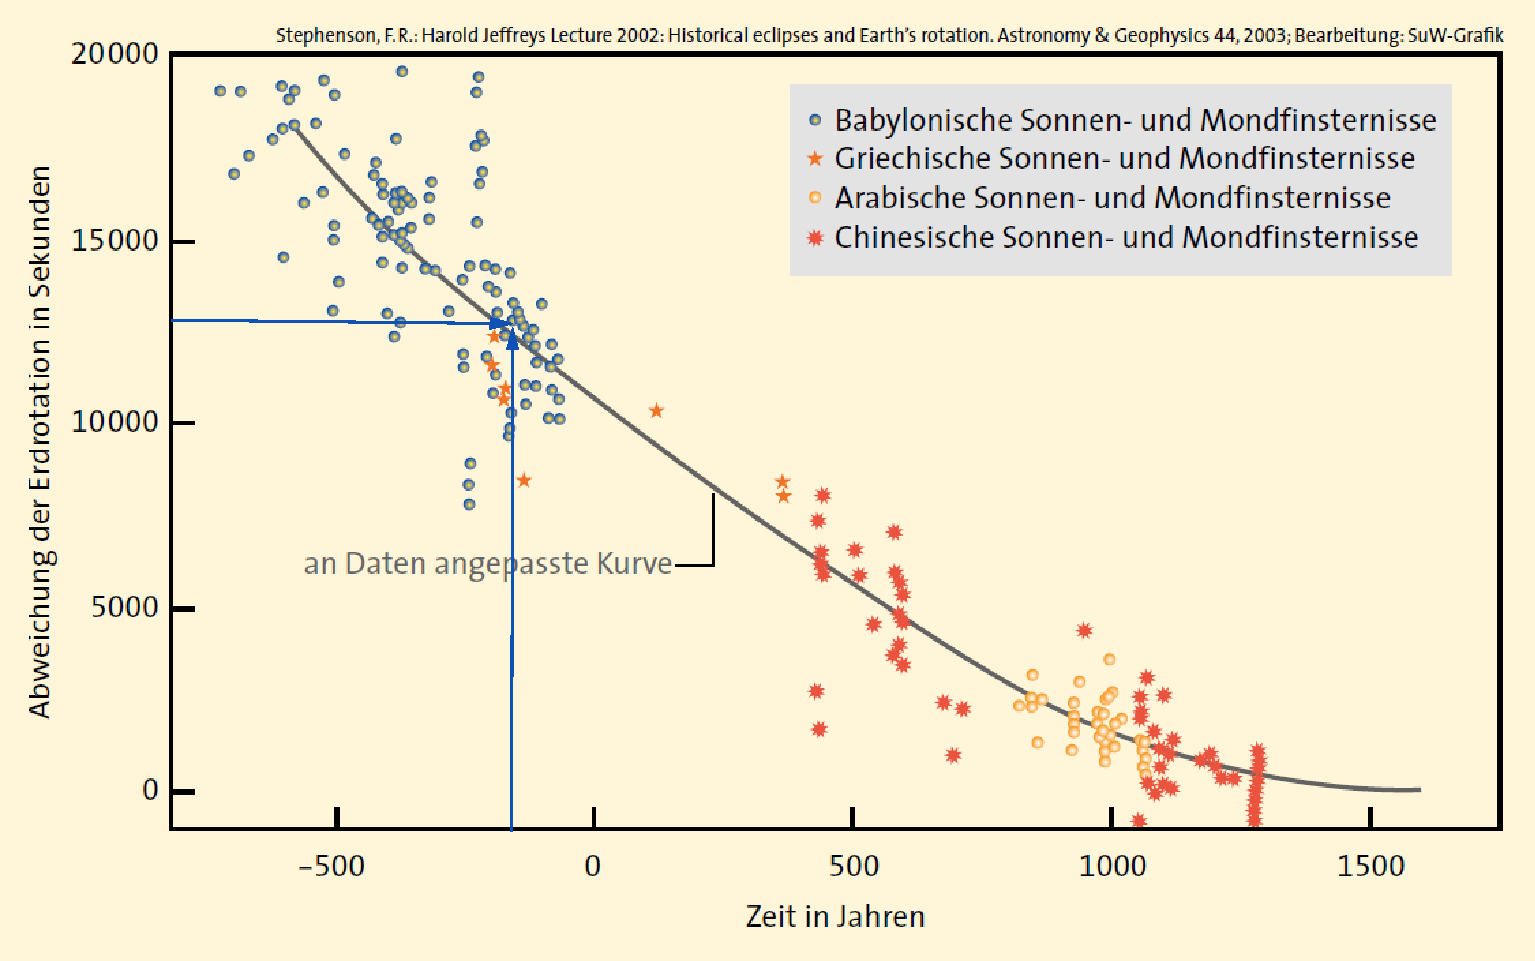
\includegraphics[width=\columnwidth]{SofiHistory.pdf}%
\caption[Abnahme der Rotationsgeschwindigkeit der Erde.]{Abnahme der Rotationsgeschwindigkeit der Erde aus Beobachtung von Sonnenfinsternissen \cite{Stephenson2016,Bastian2020}}%
\label{abb:hm_rotgeschw_sonnenfinsternis}% 
\end{figure}  
\begin{align*}
		\vec{L}_g =\sum \vec{L}_i = \vec{const} = \vec{L}_{\earth,\text{Rotation}} + \vec{L}_{\earth \text{/Mond},\text{Bahn}} + \vec{L}_\text{Mond, Rotation}  ~~.
\end{align*}
Die einzelnen Terme sind der Eigendrehimpuls der Erde, der Bahndrehimpuls des Mondes um die Erde und Eigendrehimpuls des Mondes, wobei wir letzteren auf Grund der Massenverh�ltnisse und der langsamen Rotation vernachl�ssigen k�nnen.
Eine Reduktion der Eigenrotations-Geschwindigkeit der Erde muss dann also zu einem Anwachsen des Bahndrehimpulses f�hren.
Da wir das Problem in einer Ebene behandeln wollen, k�nnen wir zu skalaren Gr��en �bergehen.
Der Betrag des Eigendrehimpulses der Erde ist dann gegeben durch $L_{\earth,\text{Rotation}} = J_{\earth} \omega_{\earth}$, der Bahndrehimpulsbetrag durch $L_{\earth \text{/Mond},\text{Bahn}} = m_{\text{M}} a_{\earth \text{M}} ^2 \omega_{\earth \text{M}}$.
Der Endzustand nach langer Zeit ($t \rightarrow \infty$) ist dann erreicht, wenn $ \omega_{\earth , \infty} = \omega_{\earth \text{M}, \infty}$, d.\,h. die Erde rotiert dann genau so schnell um sich, wie der Mond um die Erde.\\
Wir multiplizieren das Tr�gheitsmoment der Erde mit einem Faktor von $3/4$, da wir den Kern als dichter als den �u�eren Teil der Erdkruste annehmen, d.\,h. $		J_{\earth} = 0.75 \, \frac{2}{5} m_{\earth} R_{\earth}^2 $.
Mit den heutigen Werten f�r $m_{\earth}, m_{\text{M}}, a_{\earth \text{M}}, \omega_{\earth}$, und $\omega_{\earth {\text{M}}}$ kann man den Gesamtdrehimpuls berechnen zu:
	\begin{align*}
	L_g = \frac{3}{4} \, \frac{2}{5} \,m_{\earth} \,R_{\earth}^2 \, \omega_{\earth} + m_{\text{M}}\, a_{\earth \text{M}} ^2 \, \omega_{\earth \text{M}} \approx 3.4 \cdot 10^{34} \;\text{kg}\,\text{m}^2\,\text{s}^{-1} ~.
	\end{align*}
Da heute schon der Bahndrehimpuls bedeutend gr��er als der Eigendrehimpuls der Erde ist (Faktor $5$), wird das erst recht im Zustand der gebundenen Rotation gelten.
Wir k�nnen also schreiben:
	\begin{align}
	L_{g,\infty} \approx L_{\earth \text{M},\infty} = m_{\text{M}} \,  a_{\earth \text{M}, \infty} ^2 \, \omega_{\earth \text{M}, \infty} ~.\label{eq:hm_lsg_lges_inf}
	\end{align}
Andererseits gilt in guter N�herung das dritte Keplersche Gesetz, das wir mit $T_i=2\pi/\omega_i$ schreiben als:
	\begin{align}
	\omega_{\earth \text{M}, \infty} ^2 \, a_{\earth \text{M}, \infty} ^3 = \omega_{\earth \text{M}} ^2 \, a_{\earth \text{M}} ^3 ~.\label{eq:hm_lsg_kep3}
	\end{align}
Wir haben damit zwei Gleichungen f�r zwei Unbekannte ($\omega_{\earth \text{M}, \infty}$ und $a_{\earth \text{M}, \infty}$).
Aufgel�st ergeben diese
	\begin{align}
\omega_{\earth \text{M}, \infty} &= \omega_{\earth, \infty} \approx \frac{\omega_{\earth}^4 \, a_{\earth \text{M}} ^4 \, m_{\text{M}} ^3 }{L_g^2} \;\Rightarrow\:\frac{T_{\earth, \infty}}{T_{\earth}} \!=\!\lk \frac{\omega_{\earth, \infty}}{\omega_{\earth}} \rk ^{-1} \approx 45.3 ~,\label{eq:hm_lsg_finale_omega} \\ 
	a_{\earth \text{M}, \infty} &= \frac{L_g^2}{\omega_{\earth \text{M}}^2 \, a_{\earth \text{M}}^3 \, m_{\text{M}}^2} \; \Rightarrow\:\frac{a_{\earth \text{M}, \infty}}{a_{\earth \text{M}}} \approx 1.4 ~.\label{eq:hm_lsg_finale_abst}
	\end{align}
	Unser Erdentag wird damit zu dem Zeitpunkt der gebundenen Rotation etwa 45 mal so lang sein \eqref{eq:hm_lsg_finale_omega}, was uns eine ausgedehnte Nachtruhe verschaffen wird.
        Auf der anderen Seite wird es zwar weiterhin Sonnenbedeckungen durch den Mond geben, allerdings wegen \eqref{eq:hm_lsg_finale_abst} keine Totalfinsternisse mehr, \ldots was sehr schade ist.
        Wann es so weit sein wird, kann man ja mal unter Annahme der G�ltigkeit der Formel \eqref{eq:hm_ueb_verl_erdrot} f�r die Erdabbremsung nachrechnen.
        Wir wollten es eiegntlich gar nicht so genau wissen. Weitere Rechnungen zur Gezeitenreibung finden sich in \kap{hm_gezeitenreibung} und \probref{hm_gezeiten07}. \\
				
\end{sol}
\textcolor{blue} {$\rightarrow$ zur} \probref{hm_erdrotation}.\\
\noindent\rule[1ex]{\textwidth}{0.5pt} \newpage \newpage

%-----------------------------------------------------------------------------------------------------------

\begin{sol}{prob:hm_sideric_period_mars}\label{lsg:hm_sideric_period_mars} %�bung3
\textbf{Siderische Umlaufzeit des Mars} \\ \\
Wir benutzen die Geometrie aus \figref{hm_sideric_period_mars} und betrachten den Winkel (die heliozentrische L�ngen, die zwischen zwei Mars-Oppositionen �berstrichen wird.
Dies entspricht der messbaren synodischen Umlaufzeit $T_{\text{syn},\mars}$ des Mars.
Wir vernachl�ssigen bei unserer Betrachtung die Exzentrizit�t\footnote{Eine sch�ne Anleitung f�r die eigene Beobachtung der elliptischen Bahn des Mars und deren Ber�cksichtigung bei der Berechnung der siderischen Umlaufzeit findet sich in \cite{Krisciunas2019}.} und auch die relative Neigung der beiden Planetenbahnen.
Da die synodische Umlaufzeit des Mars gr��er als ein Erdjahr ist, ist die Winkelgeschwindigkeit $\omega_{\mars}$ des Mars kleiner ist als die der Erde $\omega_{\earth}$.
Mit den siderischen Umlaufzeiten $T_{\earth}$ und $T_{\mars}$ ergeben sich dann folgende �berstrichene Winkel (heliozentrische L�ngen) f�r die Zeit zwischen den beiden Oppositionen.
\begin{align*}
	T_{\mars} = \frac{2\pi\degree}{\omega_{\mars}} ~~\longrightarrow \;l_{\mars} = T_{\text{syn},\mars}\,\omega_{\mars} ~~\text{und} ~~
	T_{\earth} = \frac{2\pi\degree}{\omega_{\earth}} ~~\longrightarrow \;l_{\earth} = T_{\text{syn},\mars}\,\omega_{\earth} ~~. \end{align*}
\begin{figure}[H]
\centering
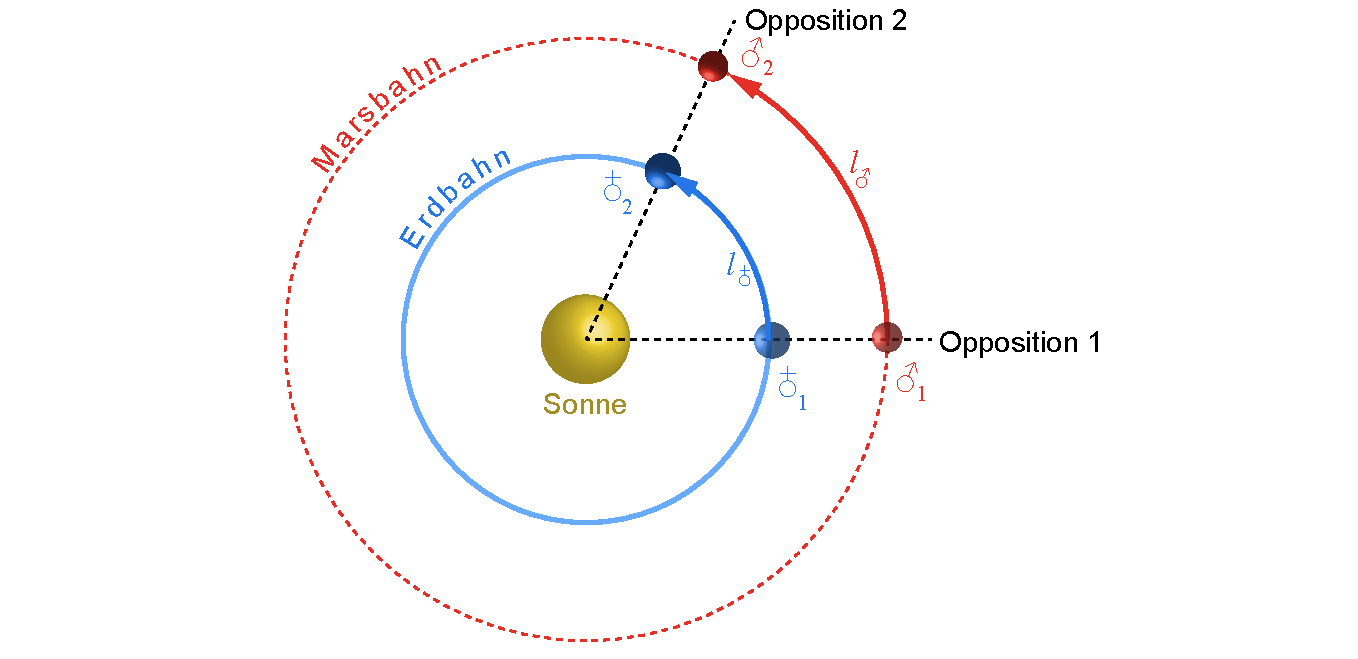
\includegraphics[width=0.9\columnwidth]{Mars_Erde_Umlauf.pdf}%
\caption{Zur Berechnung der siderischen Umlaufzeit des Mars}%
\label{abb:hm_sideric_period_mars}%
\end{figure}
Die Differenz beider L�ngen muss aber wieder $2\pi$ sein.
Daher gilt
\begin{equation*}
	\Delta l= l_{\earth} - l_{\mars} = 2\pi = T_{\text{syn},\mars} \,\lk \omega_{\earth} - \omega_{\mars}\rk = T_{\text{syn},\mars}\, 2\pi\, \lk\frac{1}{T_{\earth}}-\frac{1}{T_{\mars}}\rk ~, 
\end{equation*}
woraus mit $T_{\text{syn},\mars}\!\approx\!779.94\:\text{d}$ und $T_{\earth}\!\approx\!365.256\:\text{d}$ folgt:
\begin{align*}
T_{\mars} = \frac{{T_{\text{syn},\mars}}\, T_{\earth}}{T_{\text{syn},\mars} - T_{\earth}} = 686.980\:\text{d} ~~.\\
\end{align*}
\end{sol}
\textcolor{blue} {$\rightarrow$ zur} \probref{hm_sideric_period_mars}.\\
\noindent\rule[1ex]{\textwidth}{0.5pt} \newpage


%%%-----------------------------------------------------------------------------------------------------------

\subsection{�bungen zur Kepler-Gleichung}

\medskip

%-----------------------------------------------------------------------------------------------------------

\begin{sol}{prob:hm_laplace}\label{lsg:hm_laplace} %�bung4
\textbf{Laplace-Integral} \\
\begin{enumerate}[(i)]
	\item Wir starten von 
\begin{align*}
\vec{L} \times \ddot{\vec{r}} &= \lk \vec{r} \times \dot{\vec{r}}\rk \times \lk \frac{-\mu_\text{G}}{r^3} \rk\, \vec{r} \\
															&= \frac{\mu_\text{G}}{r^3}\,\vec{r}\times \lk \vec{r} \times \dot{\vec{r}}\rk
\end{align*}
Mit der Vektoralgebra-Beziehung 
\begin{equation*}
\vec{a}\times(\vec{b}\times\vec{c}) = \vec{b}(\vec{a}\cdot\vec{c}) - \vec{c}(\vec{a}\cdot\vec{b}) ~~.
\end{equation*}
folgt
\begin{align*}
\vec{L} \times \ddot{\vec{r}} &= \frac{\mu_\text{G}}{r^3} \lek \vec{r}(\vec{r}\cdot\dot{\vec{r}})-\dot{\vec{r}}(\vec{r}\cdot\vec{r}) \rek \\
															&= \frac{\mu_\text{G}}{r^3} \lek \vec{r}(\vec{r}\cdot\dot{\vec{r}})-\dot{\vec{r}}\,r^2\rek  ~.
\end{align*}
In Polarkoordinaten geschrieben ($\vec{r}=r\vec{e}_r$, $\dot{\vec{r}}=\dot{r}\vec{e}_r + r\dot{\vartheta}\vec{e}_\vartheta$) und wegen $\vec{e}_r\!\perp\!\vec{e}_\vartheta$ wird daraus
\begin{align}
\vec{L} \times \ddot{\vec{r}} &= \frac{\mu_\text{G}}{r^3} \lek \vec{r}(r\cdot \dot{r}) - \dot{\vec{r}}(r^2)\rek \nonumber\\
															&= \frac{\mu_\text{G}}{r^2} \dot{r}\,\vec{r} - \frac{\mu_\text{G}}{r}\,\dot{\vec{r}} = -\frac{\D}{\D t} \lk \frac{\mu_\text{G}}{r} \,\vec{r} \rk ~~.\label{eq:hm_laplace_lsg1} 
\end{align}
Die linke Seite kann wegen $\vec{L}\!=\!\vec{const}$ als Zeitableitung geschrieben werden:
\begin{equation*}
\vec{L} \times \ddot{\vec{r}} = \frac{\D }{\D t} \lk \vec{L} \times \dot{\vec{r}}\rk ~~,
\end{equation*}
woraus wir mit \eqref{eq:hm_laplace_lsg1}
\begin{align*}
\frac{\D }{\D t} \lk \vec{L}\times\dot{\vec{r}} + \frac{\mu_\text{G}}{r}\,\vec{r}\rk &= 0 
\end{align*}
erhalten.
Integration mit $-\mu_\text{G}\,\vec{e}$ als Integrationskonstante ergibt
\begin{align*}
\vec{L}\times\dot{\vec{r}} + \frac{\mu_\text{G}}{r}\,\vec{r} &= \vec{const} = -\mu_\text{G} \vec{e}
\end{align*}
und damit schlussendlich
\begin{align}
\vec{e} &= -\frac{1}{\mu_\text{G}} \lk \vec{L}\times\dot{\vec{r}} + \frac{\mu_\text{G}}{r}\,\vec{r} \rk  ~~. \label{eq:hm_laplace_lsg2}
\end{align}
\medskip
\item Wir zeigen nun, dass 
\begin{equation*}
\mu_\text{G}^2(e^2-1) = 2HL^2 ~~.
\end{equation*}
Dazu bilden wir ausgehend von \eqref{eq:hm_laplace_lsg2} das Betragsquadrat:
\begin{align*}
\lk -\mu_\text{G} \vec{e} \rk^2 &= \lk \vec{L}\times\dot{\vec{r}} + \frac{\mu_\text{G}}{r}\,\vec{r} \rk^2 \\
\Rightarrow \mu_\text{G}^2e^2 &= \lk \vec{L}\times\dot{\vec{r}} \rk^2 + \frac{2\mu_\text{G}}{r}\,\vec{r} \lk \vec{L}\times\dot{\vec{r}} \rk + \frac{\mu_\text{G}^2}{r^2}\,\vec{r}^2 \\
															&= \lek (\vec{r}\times\dot{\vec{r}})\times\dot{\vec{r}} \rek^2 + \frac{2\mu_\text{G}}{r}\,\vec{r} \lk \vec{L}\times\dot{\vec{r}} \rk + \mu_\text{G}^2 \\
															&= [\underbrace{(\vec{r}\cdot\dot{\vec{r}})\dot{\vec{r}}}_{0} - \underbrace{(\dot{\vec{r}}\cdot\dot{\vec{r}})}_{\dot{r}^2=v^2}\vec{r}]^2 + \frac{2\mu_\text{G}}{r}\,\vec{r} \lek (\vec{r}\times\dot{\vec{r}})\times\dot{\vec{r}} \rek + \mu_\text{G}^2\\
															&= v^4 r^2 + \frac{2\mu_\text{G}}{r}\,\vec{r} [ (\underbrace{\vec{r}\cdot\dot{\vec{r}})\dot{\vec{r}}}_{0} - \dot{\vec{r}}^2\vec{r} ] + \mu_\text{G}^2 \nonumber \\ 
															&= v^4 r^2 - \frac{2\mu_\text{G}}{r}\,v^2 r^2 + \mu_\text{G}^2 \nonumber 
\end{align*}															
\begin{align}													
\Rightarrow \mu_\text{G}^2 \lk e^2-1\rk &= v^4 r^2 - 2 \mu_\text{G} v^2 r ~~. \label{eq:hm_laplace_lsg3}
\end{align}
Wir benutzen jetzt die Definition $2 H\!\equiv\!v^2-(2\mu_\text{G}/r)$ und $L\!=\!\abs{\vec{L}}\!=\!\abs{\vec{r}\times \vec{v}}\!=\! rv$ und erhalten als Zwischenergebnis
\begin{align*}
2HL^2 = \underbrace{\lk v^2 - \frac{2\mu_\text{G}}{r}\rk}_{2 H} \underbrace{\lk r^2 v^2\rk}_{L^2} = v^4r^2 - 2\mu_\text{G}v^2 r ~~.
\end{align*}
was wir in \eqref{eq:hm_laplace_lsg3} einsetzen, woraus schlie�lich folgt:
\begin{equation*}
\mu_\text{G}^2 \lk e^2-1\rk  = 2 HL^2~~.
\end{equation*}
\end{enumerate}
\end{sol}
\textcolor{blue} {$\rightarrow$ zur} \probref{hm_laplace}.\\
\noindent\rule[1ex]{\textwidth}{0.5pt} \newpage

%-----------------------------------------------------------------------------------------------------------

\begin{sol}{prob:hm_wahre_anomalie}\label{lsg:hm_wahre_anomalie} %�bung5
\textbf{Wahre Anomalie}\\ \\
Wir starten von der Definition der exzentrischen Anomalie \eqref{eq:hm_exzentrische_Anomalie}:
\begin{equation*}
r(t) = a \lk 1-e\,\cos E\rk 
\end{equation*}
und benutzen dann \figref{hm_geom_abl_kepler}, so dass
\begin{align}
\overline{\text{NZ}} \equiv \overline{x}_\text{P} &= \overline{\text{ON}} - \overline{\text{OZ}} \nonumber\\
																						 &= a\cos E - ae \nonumber\\
																						 &= a (\cos E -e) \nonumber\\
\Rightarrow \cos\upsilon = 	\frac{\overline{x}_\text{P}}{r} &= \frac{\cos E-e}{1-e\cos E} ~~. \label{eq:hm_wa_lsg1}
\end{align}
Zun�chst schreiben wir \eqref{eq:hm_wa_lsg1} um in
\begin{align}
1-\cos \upsilon &= \frac{1-e\cos E - \cos E + e}{1-e\cos E} = \frac{(1+e)(1-\cos E)}{1-e\cos E} ~~, \label{eq:hm_wa_lsg2}\\
1+\cos \upsilon &= \frac{1-e\cos E + \cos E - e}{1-e\cos E} = \frac{(1-e)(1+\cos E)}{1-e\cos E} ~~. \nonumber
\end{align}
Um auf den halben Winkel in \eqref{eq:hm_nu(t)_alternativ} zu kommen, nutzen wir die Winkelfunktionsbeziehungen
\begin{align*}
1-\cos x &= 2\sin^2\lk\frac{x}{2}\rk ~~, \\
1+\cos x &= 2\cos^2\lk\frac{x}{2}\rk ~~ 
\end{align*}
und benutzen diese in \eqref{eq:hm_wa_lsg2}.
Wir erhalten sofort nach Quotientenbildung und Wurzelziehen
\begin{align*}
\lk 1 - e\, \cos E\rk \;2 \sin^2\lk\frac{\upsilon}{2}\rk &= 2(1+e)\sin^2\lk\frac{E}{2}\rk ~~,\\
\lk 1 - e\, \cos E\rk \;2 \cos^2\lk\frac{\upsilon}{2}\rk &= 2(1-e)\cos^2\lk\frac{E}{2}\rk ~~,\\
   \rightarrow~~ \tan\lk\frac{\upsilon}{2}\rk &= \sqrt{\frac{1+e}{1-e}}\,\tan\lk\frac{E}{2}\rk~~.
\end{align*}
\end{sol}
\textcolor{blue} {$\rightarrow$ zur} \probref{hm_wahre_anomalie}.\\
\noindent\rule[1ex]{\textwidth}{0.5pt} \newpage

%-----------------------------------------------------------------------------------------------------------

\begin{sol}{prob:hm_bwglg_hyp_parab}\label{lsg:hm_bwglg_hyp_parab} %�bung6
\textbf{Bewegungsgleichungen f�r Hyperbel und Parabel} \\
\begin{enumerate}[(i)]
	\item \emph{Hyperbel}\\
	Diese Herleitung erfolgt analog zur Kepler-Gleichung f�r die Ellipse.
        Man f�hrt lediglich anstelle der Hilfsgr��e \anf{exzentrische Anomalie} eine \anf{hyperbolische exzentrische Anomalie} $E_\text{hyp}$ ein.
        Man beachte dabei, dass bei einer Hyperbel $a\!<\!0$ ist.
        Zudem ben�tigen wir f�r die weitere Rechnung folgende Beziehungen f�r Hyperbelfunktionen:
\begin{align*}
\sinh^2x &= \cosh^2x-1 ~~, \\
\sinh x &= \frac{\D }{\D x} \cosh x ~~,\\
\cosh x &= \frac{\D }{\D x} \sinh x ~~.
\end{align*}
Wir starten zun�chst mit
\begin{align}
r &= a_\text{hyp} (1-e\cosh E_\text{hyp}) \nonumber \\
  &= \abs{a_\text{hyp}} (e\cosh E_\text{hyp} - 1) \label{eq:hm_hyplsg1} 
\end{align}
und bilden die zeitliche Ableitung, die wir anschlie�end quadrieren:
\begin{align}
\frac{\D r}{\D t} =&\, +\abs{a_\text{hyp}}e \sinh E_\text{hyp}\,\lk\frac{\D E_\text{hyp}}{\D t}\rk  \nonumber \\ 
\lk\frac{\D r}{\D t}\rk^2 =&\, +\, \abs{a_\text{hyp}}^2 e^2 (\sinh E_\text{hyp})^2 \,\lk\frac{\D E_\text{hyp}}{\D t}\rk^2 ~.\label{eq:hm_hyplsg2}
\end{align}
Dann starten wir wieder mit der Bahngeschwindigkeit in Polarkoordinaten und benutzen \eqref{eq:hm_dot_r_quadrat}, so dass
\begin{align*}
\lk\frac{\D r}{\D t}\rk^2 =&\, \frac{\mu_\text{G}}{r^2} \lk 2r-\frac{r^2}{a_\text{hyp}}\rk -\lk \frac{a_\text{hyp}(1-e^2)}{r^2} \rk\,\mu_\text{G} ~~.
\end{align*}
Wir setzen jetzt f�r $r$ die Beziehung \eqref{eq:hm_hyplsg1} ein und erhalten 
\begin{align*}
\lk\frac{\D r}{\D t}\rk^2 =&\, \frac{\mu_\text{G}}{r^2} \lk \killA{2\abs{a_\text{hyp}} e \cosh E_\text{hyp}} - \killB{2 \abs{a_\text{hyp}}} +\frac{\abs{a_\text{hyp}}^2}{\abs{a_\text{hyp}}} e^2 \cosh^2 E_\text{hyp} \right.\\
&\,\left. +\killB{\frac{\abs{a_\text{hyp}}^2}{\abs{a_\text{hyp}}}} - \killA{\frac{2\abs{a_\text{hyp}}^2}{\abs{a_\text{hyp}}}e\cosh E_\text{hyp}} + \killB{\abs{a_\text{hyp}}} -\abs{a_\text{hyp}} e^2\rk \\
=&\, \frac{\mu_\text{G}}{r^2} \lk \abs{a_\text{hyp}} e^2 \cosh^2 E_\text{hyp} - \abs{a_\text{hyp}} e^2\rk \\
=&\, \frac{\mu_\text{G}}{r^2} \abs{a_\text{hyp}} e^2 \underbrace{\lk \cosh^2 E_\text{hyp} - 1\rk}_{\sinh^2 E_\text{hyp}} ~~, 
\end{align*}
und weiter mit \eqref{eq:hm_hyplsg2}
\begin{align*}
\abs{a_\text{hyp}}^{\killA{2}} \killA{e^2 \sinh^2 E_\text{hyp}} \,\lk \frac{\D E_\text{hyp}}{\D t}\rk^2 &= \frac{\mu_\text{G}}{r^2} \killA{\abs{a_\text{hyp}} e^2 \sinh^2 E_\text{hyp}} \\
\Rightarrow r \lk \frac{\D E_\text{hyp}}{\D t}\rk &= \sqrt{\frac{\mu_\text{G}}{\abs{a_\text{hyp}}}} ~~.
\end{align*}
Wir setzen wieder f�r $r$ die Beziehung \eqref{eq:hm_hyplsg1} ein und bekommen
\begin{align*}
\abs{a_\text{hyp}} (e\cosh E_\text{hyp} - 1)\,\D E_\text{hyp} &= \sqrt{\frac{\mu_\text{G}}{\abs{a_\text{hyp}}}} \,\D t ~~,
\end{align*}
woraus nach Integration 
\begin{align}
e \sinh E_\text{hyp} - E_\text{hyp}  &= \sqrt{\frac{\mu_\text{G}}{\abs{a_\text{hyp}}^3}} (t-t_0) = M_\text{hyp}(t-t_0) ~~  \label{eq:hm_hyplsg3}
\end{align}
eine hyperbolische modifizierte Kepler-Gleichung resultiert.
Die L�sung dieser Gleichung erfolgt ebenfalls numerisch durch Iteration oder Reihenentwicklung.\\

\item \emph{Parabel}\\
Bei der Parabel ist die Situation interessanterweise etwas einfacher.
Wir wissen ja, dass f�r die Parabel $e\!=\!1$ ist.
Somit arbeiten wir mit dem Parameter $p$.
Wir starten von der Kegelschnittgleichung \eqref{eq:hm_kegelschnitt}:
\begin{equation*}
r(\upsilon) = \frac{L^2}{\mu_\text{G}}\,\frac{1}{1+\cos \upsilon} = \frac{p}{1+\cos \upsilon} ~~.
\end{equation*}
Andererseits ist noch wegen \eqref{eq:hm_drehimp_z} $L\!=\!r^2\dot{\upsilon}$, so dass wir fortfahren mit
\begin{align*}
\frac{\D \upsilon}{\D t} &= \frac{L}{r^2} \Rightarrow r^4\,\lk\frac{\D \upsilon}{\D t}\rk^2 = L^2 = \mu_\text{G}p \\
\Rightarrow \frac{\D \upsilon}{\D t} &= \sqrt{\mu_\text{G} p} \lk\frac{1}{r^2}\rk = \sqrt{\mu_\text{G} p}\,\lk\frac{(1+\cos\upsilon)^2}{p}\rk^2 \\
\Rightarrow \D \upsilon &= \sqrt{\frac{mu_\text{G}}{p^3}} \lek 2\cos^2\lk\frac{\upsilon}{2}\rk\rek^2 \,\D t ~~,
\end{align*}
wobei wir in der letzten Zeile die Beziehung $1+\cos x\!=\!2\cos^2(x/2)$ verwendet haben.
Damit erhalten wir nach Trennung der Variablen
\begin{equation*}
\frac{1}{2} \lk \,\frac{1}{\cos^4 \lk\frac{\upsilon}{2}\rk} \rk\,\D \lk\frac{\upsilon}{2}\rk  = \sqrt{\frac{\mu_\text{G}}{p^3}}\,\D t ~~.
\end{equation*}
In Integraltabellen findet man $\int (\cos^{-4} u)\,\D u \!=\! \tan u + (1/3)\tan^3 u + c$, was man leicht durch Differenzieren pr�fen kann.
Damit erhalten wir nun eine Bestimmungsgleichung f�r $\upsilon$:
\begin{equation*}
\tan\lk\frac{\upsilon}{2}\rk + \frac{1}{3}\tan^3\lk\frac{\upsilon}{2}\rk = 2 \sqrt{\frac{\mu_\text{G}}{p^3}} (t-t_0)~~.
\end{equation*}
Aus der Parabelgleichung folgt f�r $\upsilon\!=\!0$ die Periheldistanz $q$ zu
\begin{equation*}
q = \frac{p}{1+\cos(0)} = \frac{p}{2}
\end{equation*}
und daraus die sogenannte Barkersche Gleichung f�r die wahre Anomalie der Bahn der Parabel
\begin{equation}
\tan\lk\frac{\upsilon}{2}\rk  + \frac{1}{3} \tan^3\lk\frac{\upsilon}{2}\rk  = \sqrt{\frac{4\mu_\text{G}}{8q^3}} (t-t_0) = \sqrt{\frac{\mu_\text{G}}{2q^3}} (t-t_0)~~.
\label{eq:hm_BarkerGleichung01}
\end{equation}
Das ist noch eine transzendente Gleichung in $\upsilon$.
Setzt man aber $\tan(\upsilon/2)\!=\!u$, so wird daraus
\begin{equation}
u+\frac{1}{3}u^3 = M_\text{P}(t-t_0)~~, \label{eq:hm_BarkerGleichung02}
\end{equation}
gl�cklicherweise eine mit den bekannten Formeln f�r kubische Gleichungen analytisch l�sbare Form.
Mit
\begin{equation*}
A = \frac{3}{2} \sqrt{\frac{\mu_\text{G}}{2q^3}} (t-t_0)A ~~~\text{und}~~~B = \sqrt[3]{A+\sqrt{A^2+1}}
\end{equation*}
findet man:
\begin{equation}
   \upsilon = 2\arctan{(\lk b - \frac{1}{B}\rk }\,. \label{eq:hm_BarkerGleichung03}
\end{equation}

Im Gegensatz zur Ellipse und Hyperbel hat also der Spezialfall der Parabel\index{Parabel} eine geschlossene analytische L�sung.
Wir werden dieser Barkerschen Gleichung\index{Barkersche Gleichung} in modifizierte Form bei der Berechnung von Kometenbahnen wieder begegnen.
\end{enumerate}
\end{sol}
\textcolor{blue} {$\rightarrow$ zur} \probref{hm_bwglg_hyp_parab}.\\
\noindent\rule[1ex]{\textwidth}{0.5pt} \newpage

%-----------------------------------------------------------------------------------------------------------

\begin{sol}{prob:hm_iteration}\label{lsg:hm_iteration} %�bung7
\textbf{Iteration} \\ \\
Die Rechnungen sind im Detail in \mlhmref{KeplerVergleich.m} ausgef�hrt. 
\end{sol}
\textcolor{blue} {$\rightarrow$ zur} \probref{hm_iteration}.\\
\noindent\rule[1ex]{\textwidth}{0.5pt} \newpage

%-----------------------------------------------------------------------------------------------------------

\begin{sol}{prob:hm_bessel}\label{lsg:hm_bessel} %�bung8
\textbf{Bessel-Reihe} \\ \\
Die Rechnungen sind im Detail im \mscr{} \mlhmref{Besselreihe.m} ausgef�hrt. 
\end{sol}
\textcolor{blue} {$\rightarrow$ zur} \probref{hm_bessel}.\\
\noindent\rule[1ex]{\textwidth}{0.5pt} \newpage

%-----------------------------------------------------------------------------------------------------------

\begin{sol}{prob:hm_alternative_MPG}\label{lsg:hm_alternative_MPG} %�bung9
\textbf{Alternative Herleitung der Mittelpunktsgleichung} \\ \\
Im Beispiel \ref{bsp:mittelpktglg} hatten wir die Mittelpunktsgleichung �ber die Bessel-Reihe hergeleitet.
Wir wollen hier nun Herleitung �ber die Iterationsl�sung nach Kapitel \ref{kap:iteration_kepler} wiederholen und folgen dabei der eleganten Darstellung in \cite{Smart1986}. Wir starten mit \eqref{eq:hm_nu(t)_alternativ} (siehe auch \probref{hm_wahre_anomalie}):
\begin{equation*}
\tan \lk \frac{\upsilon}{2} \rk = \sqrt{\frac{1+e}{1-e}}\,\tan\lk\frac{E}{2}\rk ~~.
\end{equation*}
Wir setzen $\sin\alpha\!=\!e$, da $0\!\leq\! e\!\leq\! 1$, was aus $0\!\leq\!\alpha\!\leq\!\pi$ folgt.
Mit der Identit�t 
\begin{align*}
1 \pm \sin\alpha &= 1 \pm \frac{2 \tan\lk\frac{\alpha}{2}\rk}{1+\tan^2\lk\frac{\alpha}{2}\rk} = \frac{1 \pm 2 \tan\lk\frac{\alpha}{2}\rk+\tan^2\lk\frac{\alpha}{2}\rk}{1+\tan^2\lk\frac{\alpha}{2}\rk} \\
                 &= \frac{{\lk 1 \pm \tan\lk\frac{\alpha}{2}\rk \rk}^2}{1+\tan^2\lk\frac{\alpha}{2}\rk}
\end{align*}
erh�lt man
\begin{equation}
\tan \lk \frac{\upsilon}{2} \rk  = \frac{1+\tan\lk\frac{\alpha}{2}\rk}{1-\tan\lk\frac{\alpha}{2}\rk}\,\tan\lk\frac{E}{2}\rk = \frac{1+x}{1-x}\,\tan\lk\frac{E}{2}\rk~~. \label{eq:hm_lsg_mpg_1}
\end{equation}
Wir benutzen nun die Euler-Gleichungen $\cos\theta\!=\!1/2 \lk \E^{\im\theta}+\E^{-\im\theta}\rk$ und $\sin\theta\!=\!1/(2\im)\lk\E^{\im\theta}-\E^{-\im\theta}\rk$ und schreiben mit dem Tangens des halben Winkels $\upsilon$ und analog f�r den Tangens des halben Winkel $E$ die Beziehung f�r die wahre Anomalie als
\begin{equation*}
\tan \lk \frac{\upsilon}{2} \rk = \frac{\E^{+\im\upsilon/2} - \E^{-\im\upsilon/2}}{i\lk\E^{+\im\upsilon/2} + \E^{-\im\upsilon/2}\rk} = \frac{\E^{\im\upsilon}-1}{i\lk \e^{\im\upsilon} + 1\rk} \frac{\killA{\E^{-\im\upsilon/2}}}{\killA{\E^{-\im\upsilon/2}}}~~,
\end{equation*}
woraus mit \eqref{eq:hm_lsg_mpg_1} folgt
\begin{equation}
\frac{\E^{\im\upsilon}-1}{\E^{\im\upsilon}+1} = \frac{1+x}{1-x}\,\frac{\E^{\im E}-1}{\E^{\im E}+1}~~.
\label{eq:hm_lsg_mpg_2}
\end{equation}
Wir setzen nun $\E^{\im\upsilon}\!\equiv\!\E^q$ und die rechte Seite gleich $Q$.
Damit ergibt sich vereinfacht
\begin{align}
\E^q -1 &= Q\lk \E^q+1\rk \nonumber\\
\E^q \lk 1-Q\rk &= Q+1  \nonumber\\
\Rightarrow \E^{\im \upsilon} &= -\frac{Q+1}{Q-1} = \frac{\E^{\im E}-x}{1-x\E^{\im E}} \nonumber\\
															 &= \E^{\im E} \lk \frac{1-x\E^{-\im E}}{1-x\E^{+\im E}} \rk ~~. \label{eq:hm_lsg_mpg_3}
\end{align}
Wir bilden davon den Logarithmus und erhalten
\begin{equation}
\im\upsilon = \im E + \ln\lk1-x\E^{-\im E}\rk - \ln\lk1-x\E^{+\im E}\rk ~~.
\label{eq:hm_lsg_mpg_4}
\end{equation}
Da $x\!=\!\tan(\alpha/2)$ und $\alpha\!=\!\arcsin(e)$, ist $\alpha$ definitiv kleiner als $\pi/2$ und damit $0\!<\!x^e\!<\!1$.
Wir benutzen jetzt die Reihenentwicklung $\ln(1-z)\!=\!z-z^2/2-z^3/3-z^4/4-\ldots$ und erhalten 
\begin{align}
\im\upsilon &= \im E + x\E^{\im E} - x\E^{-\im E} + \frac{x^2}{2}\E^{2\im E} - \frac{x^2}{2}\E^{-2\im E} + \frac{x^3}{3}\E^{3\im E} - \frac{x^3}{3}\E^{-3\im E} - \ldots \nonumber\\
\Rightarrow \im\upsilon &= \im \lek E + \lk 2x\sin E + x^2 \sin(2E) + \frac{2}{3} x^3 \sin(3E) + \ldots \rk \rek~~. \label{eq:hm_lsg_mpg_5}
\end{align}
Jetzt m�ssen wir noch $x$ re-substituieren gem��
\begin{equation*}
x = \tan\lk\frac{\alpha}{2}\rk = \frac{\sin^2\lk\frac{\alpha}{2}\rk}{\sin\lk\frac{\alpha}{2}\rk \cos\lk\frac{\alpha}{2}\rk} = \frac{1-\cos^2\lk\frac{\alpha}{2}\rk}{\frac{1}{2}\sin\alpha} = \frac{2\lk1-\cos^2\lk\frac{\alpha}{2}\rk\rk}{e} ~~.
\end{equation*}
Wiederum benutzen wir die Identit�t $2\,\cos^2(\alpha/2)\!=\!(1+\cos\alpha)$ und erhalten
\begin{equation*}
x = \frac{1-\cos\alpha}{e} = \frac{1-\sqrt{1-\sin^2\alpha}}{e} = \frac{1-\sqrt{1-e^2}}{e} ~~.
\end{equation*}
Wir entwickeln nun den Ausdruck in der Wurzel nach kleinen $e$:
\begin{align*}
x &= \frac{1}{e} \lk 1- \lk 1-\frac{e^2}{2} - \frac{e^4}{8} - \frac{e^6}{16} - \ldots \rk\rk \\
  &= \frac{e}{2} + \frac{e^3}{8} + \frac{e^5}{16} + \ldots ~~.
\end{align*}
Dies setzen wir nun in \eqref{eq:hm_lsg_mpg_5} ein und erhalten schlie�lich bis zur 3. Ordnung von $e$
\begin{equation}
\upsilon = E + \lk e+\frac{e^3}{4} \rk\sin(E) + \frac{e^2}{4} \sin(2E) + \frac{e^3}{12} \sin(3E) + \mathcal{O}(e^4) ~~.
\label{eq:hm_lsg_mpg_6}
\end{equation}
Nun m�ssen wir noch die Sinus-Werte der unbekannten exzentrischen Anomalie $E$ durch die bekannte mittlere Anomalie $M$ ausdr�cken, um die gesuchte Gleichung f�r $\upsilon-M$ zu erhalten.
Dazu nutzen wir das Iterationsergebnis \eqref{eq:hm_entwicklung_4Ord}, brauchen aber nur die Entwicklung bis $e^2$, da in \eqref{eq:hm_lsg_mpg_6} alle $\sin kE$-Funktionen mindestens mit $e$ multipliziert werden.
Wir bekommen
\begin{equation}
E = M+\lk e-\frac{e^3}{8}\rk\sin(M) + \frac{e^2}{2}\sin(2M) + \frac{3}{8} e^3\sin(3M) + \ldots ~~.
\label{eq:hm_lsg_mpg_7}
\end{equation}
Wir brauchen aber nur Terme bis zur Ordnung $e^2$ mitzunehmen, da in \eqref{eq:hm_lsg_mpg_5} mindestens mit der Potenz 1 vo $e$ multipliziert wird. Wir k�nnen also schreiben:
\begin{equation*}
\sin E \approx \sin\lk M+e\sin(M) +\frac{e^2}{2}\sin(2M)\rk \,.
\end{equation*}
Mit der N�herung f�r kleine Winkel\\
$\sin x\!\approx\!x$, $\cos x\!\approx\!1-\frac{1}{2}x^2$,
den Additionstheoremen der Trigonometrie und der Beziehung $\sin^3 x = \frac{3}{4}\sin x -\frac{1}{4}\sin(3x) $ ergibt das dann in Ordnungen bis $e^2$:
\begin{align*}
\sin(E)  &= \sin(M)\, \cos\lk e\sin(M) +\frac{e^2}{2}\sin(2M)\rk + \cos(M)\,\sin\lk e\sin(M) +\frac{e^2}{2}\sin(2M)\rk \\
         &\approx \sin(M)\,\lek 1- \frac{1}{2}e^2\sin^2(M) \rek + \cos(M)\,\lek e\sin(M)+\frac{e^2}{2}\sin(2M) \rek \\
         &= \sin(M) + \frac{1}{2}e\sin(2M) + \frac{e^2}{2} \lek \sin(2M)\cos(M) - \sin^3(M) \rek \\
         &= \lk 1- \frac{e^2}{8} \rk \sin(M) + \frac{1}{2}e\sin(2M)  + \frac{3}{8}e^2\sin(3M) \,.
\end{align*}
Analog erhalten wir:
\begin{align*}
\sin(2E) &\approx \sin(2M) + e(\sin(3M) - \sin M)\,, \\
\sin(3E) &\approx \sin 3M ~~.
\end{align*}
Die $\sin(E),\, \sin(2E),\, \sin(3E)$-N�herungen setzen wir in \eqref{eq:hm_lsg_mpg_6} ein und erhalten schlie�lich die Mittelpunktsgleichung \eqref{eq:hm_mpglg_nu-M} bis zur Ordnung $e^3$:
\begin{equation*}
\upsilon-M = \lk 2e-\frac{e^3}{2}k \rk\sin(M) + \frac{5e^2}{4} \sin(2M) + \frac{13e^3}{12}\sin(3M) ~~.
\end{equation*}
Auch hier empfehlen wir als weitere �bung die Entwicklung bis mindestens zum Term mit $e^4$ bzw. $\sin(4M)$ zu berechnen.\\
\end{sol}
\textcolor{blue} {$\rightarrow$ zur} \probref{hm_alternative_MPG}.\\
\noindent\rule[1ex]{\textwidth}{0.5pt} \newpage


%%%-----------------------------------------------------------------------------------------------------------

\subsection{�bungen zur Bewegung der Erde in der Ekliptik und zu Himmelsbeobachtungen von der Erde}

\medskip

%-----------------------------------------------------------------------------------------------------------

\begin{sol}{prob:hm_erdbahn_im_jahr}\label{lsg:hm_erdbahn_im_jahr} %�bung10
\textbf{Die Erdbahn im Laufe eines Jahres} \\
\begin{enumerate}[(1)]
	\item Die Perihel- bzw. Apheldistanzen berechnen sich zu
	\begin{align*}
  r_\text{per} &= \frac{p}{1+e\cos\upsilon}\bigg|_{\upsilon=0} = \frac{a(1-e^2)}{1+e} = a(1-e) \approx 147.098\cdot 10^6\:\text{km} ~~,\\
	 r_\text{aph} &= \frac{p}{1+e\cos\upsilon}\bigg|_{\upsilon=\pi} = a(1+e) \approx 152.098\cdot 10^6\:\text{km} ~~.
	\end{align*}
	Die Erdentfernung schwankt also um insgesamt $5\cdot 10^6\:$km.
	\item Wir wollen die mittlere Entfernung berechnen.
          Dazu gibt es zwei M�glichkeiten: den \emph{r�umlichen} Mittelwert der Entfernung zwischen Brennpunkt (Sonne) und Bahn und den \emph{zeitlichen} Mittelwert. 
		\begin{itemize}
		\item Wir beginnen mit dem r�umlichen Mittelwert und schreiben
		 \begin{align}
			\bar{r} &= \frac{1}{2\pi} \int\limits_{0}^{2\pi} r(\upsilon)\,\D\upsilon= \frac{p}{2\pi}\,2\,\int\limits_0^\pi \frac{1}{1+e\cos \upsilon}\,\D\upsilon \label{eq:hm_erdbahn_lsg_1} \\
			         &\stackrel{\text{\cite{Gradshteyn1980}}}{=} \frac{p}{\pi}\,\frac{2}{\sqrt{1-e^2}}\,\arctan\lk \sqrt{\frac{1-e}{1+e}} \,\underbrace{\tan\lk \frac{\upsilon}{2}\rk}_{\rightarrow\infty} \rk\Bigg|_0^\pi = \frac{2p}{\pi\sqrt{1-e^2}} \,\underbrace{\arctan(\infty)}_{\rightarrow\pi/2} \nonumber \\
                                 &= \frac{p}{\sqrt{1-e^2}} = \frac{a(1-e^2)}{\sqrt{1-e^2}} = a\sqrt{\frac{(1-e^2) \killA{(1-e^2)}}{\killA{(1-e^2)}}} = a\sqrt{1-e^2} = b ~~.\nonumber
		 \end{align}
		Dieser Mittelwert ist also gleich der kleinen Halbachse.
		\item Wir berechnen jetzt den zeitlichen Mittelwert unter Benutzung von $T\!=\!T_\text{sid}$:
	\begin{align}
	\bar{r}^t &= \frac{1}{T_\text{sid}} \int\limits_{0}^{T_\text{sid}} r(t)\,\D t = \frac{1}{T}\int\limits_0^{2\pi} r(\upsilon) \,\underbrace{\frac{\D t}{\D \upsilon}}_{1/\dot{\upsilon}}\,\D\upsilon = \frac{1}{T}\int\limits_0^{2\pi} \frac{r(\upsilon)}{\dot{\upsilon}}\,\D\upsilon ~.\label{eq:hm_erdbahn_lsg_2}
	\end{align}
Unter Benutzung des Drehimpulssatzes $1/\dot{\upsilon}\!=\!r^2/L$ erh�lt man zun�chst
		\begin{equation*}
		\bar{r}^t = \frac{1}{TL} \int\limits_0^{2\pi} r^3(\upsilon)\,\D\upsilon = \frac{1}{TL}\int\limits_0^{2\pi} \frac{p^3}{(1+e\cos\upsilon)^3}\,\D\upsilon = \frac{2p^3}{TL}\int\limits_0^{\pi} \frac{1}{(1+e\cos\upsilon)^3}\,\D\upsilon ~~.
		\end{equation*}
		Mit den Integraltabellen aus \cite{Gradshteyn1980} ergibt sich damit
		\begin{equation}
		\bar{r}^t = \frac{2p^3}{TL}\,\pi\,\frac{\lk 1+\frac{e^2}{2}\rk}{(1-e^2)^{5/2}} ~~. \label{eq:hm_erdbahn_lsg_4}
		\end{equation}
		Wir benutzen jetzt den Fl�chensatz f�r einen ganzen Umlauf $TL\!=\! 2A_\text{Ellipse}\!=\!2\pi\,a b$.
                Mit \eqref{eq:hm_erdbahn_lsg_4} erhalten wir dann unter Benutzung von $\sqrt{1-e^2}\!=\!b/a$
		\begin{align*}
		\bar{r}^t =&\, \frac{\killA{2}p^3}{\killA{2\pi} ab}\,\killA{\pi}\,\lk 1+\frac{e^2}{2}\rk \frac{a^5}{b^5} = \, \frac{a^7 \lk\sqrt{1-e^2}\rk^6}{b^6}\,\lk 1+\frac{e^2}{2}\rk\\
							=&\, \frac{a \overbrace{\lek a \sqrt{1-e^2}\rek^6}^{=b^6}}{b^6}\,\lk 1+\frac{e^2}{2}\rk = \, a \lk 1+\frac{e^2}{2}\rk ~\\
						\text{mit}~ p =& a(1-e^2) ~.
		\end{align*}
Das hei�t, dass die Erde im zeitlichen Mittel mehr als $1\:$AE entfernt ist und zwar um $20886\:$km.
Die kleinere Geschwindigkeit am Aphel f�hrt zu einem l�ngeren Aufenthalt im dortigen Bereich.
	\end{itemize}
	\item Die Jahreszeiten sind kein Effekt der Elliptizit�t der Bahn, sondern werden prim�r durch die Ekliptikneigung und - pr�zession hervorgerufen.
          Wir betrachten dazu die \figref{hm_erdbahn_lsg_1}, in der wir die Projektion der Erdachse auf die Bahnebene (Ekliptik) zeigen.\footnote{Der Richtungseinheitsvektor der Erdachse $\vec{s}_{\text{rot},\earth}$ hat die Komponenten $s_{\text{rot},x}\!=\!\sin\epsilon\cos\alpha$, $s_{\text{rot},y}\!=\!\sin\epsilon\sin\alpha$ und $s_{\text{rot},z}\!=\!\cos\epsilon$, wobei $\alpha$ der Winkel ist, den die Projektion der Erdachse auf die Ekliptik mit der $x$-Achse bildet.
          Die Projektion der Erdachse auf die Ekliptik $\vec{s}_{\text{ek}}$ zeigt also in Richtung des Vektors Sonne zur Position der Wintersonnnenwende.} Definitionsgem�� steht zum �quinoktium die Achse dann in ihrer Ausrichtung senkrecht zur Sonne (\ldots wir schauen von oben auf die Bahnebene). 
\begin{figure}[H]
\centering
	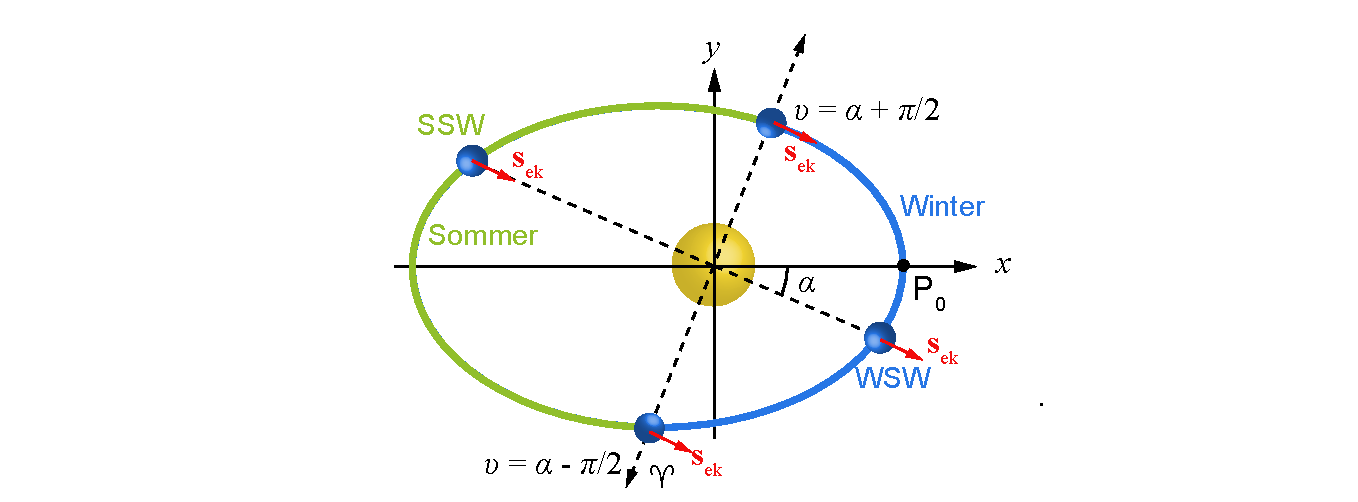
\includegraphics[width=\textwidth]{Erdbahn_im_Jahr_lsg2.pdf}%
	\caption{Erdbahn im Jahresverlauf}%
	\label{abb:hm_erdbahn_lsg_1}%
\end{figure}

	Wir definieren jetzt:
	\begin{align*}
		\text{Nordwinter: }& \alpha - \frac{\pi}{2} \leq \upsilon \leq \alpha+\frac{\pi}{2} ~~,\\
		\text{Nordsommer: }& \alpha + \frac{\pi}{2} \leq \upsilon \leq \alpha+\frac{3\pi}{2} ~~.
	\end{align*}
	Diese Halbjahre sind durch die Richtung der Erdachse gegeben und sind keineswegs gleich lang, wie wir gleich berechnen werden.
        Der gesamte Umlauf ben�tigt nach dem 3. Keplerschen Gesetz $T_\text{ges}\!=\!2\pi \sqrt{a^3/\mu_\text{G}}$.
        Die zeitliche Dauer des Sommerhalbjahrs ergibt sich dann mit Nutzung der Beziehungen
	\begin{align*}
		\frac{\D\upsilon}{\D t} &= \frac{L}{r^2} ~~\text{bzw.} ~~ \D t = \frac{r^2\,\D\upsilon}{L} ~,\;L = \sqrt{a\mu_\text{G}(1-e^2)} ~ \text{und}\;	r^2 = \lek \frac{a(1-e^2)}{1+e\cos\upsilon} \rek^2 ~~
	\end{align*}
	zu
	\begin{align}
   T_\text{Sommer} &= \frac{1}{L} \int\limits_{\alpha+\pi/2}^{\alpha+3\pi/2} r^2 \,\D\upsilon = \frac{a^2\lk 1-e^2\rk^2}{\sqrt{a\mu_\text{G}(1-e^2)}} \,\int\limits_{\alpha+\pi/2}^{\alpha+3\pi/2} \frac{1}{\lk 1+e\cos\upsilon\rk^2}\,\D\upsilon \nonumber\\
									 &= \frac{a^{3/2}\lk 1-e^2\rk^{3/2}}{\sqrt{\mu_\text{G}}} \,\underbrace{\int\limits_{0}^{\pi} \frac{1}{\lek 1-e\sin(\varphi+\alpha)\rek^2} \,\D\varphi}_{\equiv I} ~~, \label{eq:hm_erdbahn_lsg_5}
	\end{align}
	wobei wir $\cos(x+\pi/2)\!=\!-\sin x$ verwendet und $\varphi\!=\!\upsilon-(\alpha+\pi/2)$ gesetzt haben.
        Die L�sung des Integrals $I$ in \eqref{eq:hm_erdbahn_lsg_5} k�nnten wir wieder �ber \cite{Gradshteyn1980} erledigen.
        Wir wollen aber hier f�r kleine $e$ eine Reihenentwicklung durchf�hren:
	\begin{align*}
		I =&\, \int\limits_{0}^{\pi} \frac{1}{\lek 1-e\sin(\varphi+\alpha)\rek^2} \,\D\varphi \\
		  =&\, \int\limits_{0}^{\pi} \lek 1+2e\sin(\varphi+\alpha) + 3e^2\sin^2(\varphi+\alpha) + 4e^3\sin^3(\varphi+\alpha) \rek\,\D\varphi \\
		  =&\, \pi - 2e\cos(\varphi+\alpha) \bigg|_0^\pi + 3e^2 \lek -\frac{1}{4}\sin(2(\varphi+\alpha))+ \frac{1}{2}(\varphi+\alpha) \rek_0^\pi \\
			 &\, + 4e^3 \lek \frac{1}{12}\cos(3(\varphi+\alpha)) - \frac{3}{4}\cos(\varphi+\alpha)\rek_0^\pi \\
			=&\, \pi + 4e\cos\alpha+\frac{3}{2} e^2 \pi - 4e^3\,\frac{1}{6}\cos(3\alpha) + 6e^3\cos\alpha ~~.
	\end{align*}
	Damit erhalten wir
	\begin{align}
	T_\text{Sommer} =&\, \frac{a^{3/2}}{\sqrt{\mu_\text{G}}} \lk 1-\frac{3e^2}{2} + \mathcal{O}(e^4)\rk \lk \pi + 4e\cos\alpha + \frac{3e^2}{2} \pi - \frac{2e^3}{3}\cos (3\alpha) \right.\nonumber\\
	                 &\left. + 6e^3\cos\alpha +\mathcal{O}(e^4)\rk \nonumber\\
	              =&\, \frac{a^{3/2}}{\sqrt{\mu_\text{G}}} \lek \pi - \killA{\frac{3e^2}{2} \pi} + 4e\cos\alpha + \killA{\frac{3e^2}{2} \pi} - \killB{6e^3\cos\alpha} \right.\nonumber\\
                      &\left. -\frac{2e^3}{3}\cos(3\alpha) + \killB{6e^3\cos\alpha} + \mathcal{O}(e^4) \rek \nonumber\\
								=&\, \frac{a^{3/2}}{\sqrt{\mu_\text{G}}} \lek \pi + 4e\cos\alpha - \frac{2e^3}{3}\cos(3\alpha)\rek ~~.\label{eq:hm_erdbahn_lsg_6}
	\end{align}
	Wegen $T_\text{Winter}\!=\! T_\text{ges} - T_\text{Sommer}$ ergibt sich die Differenz der beiden Halbjahre zu
	\begin{align}
		\Delta T &= \frac{T_\text{Sommer} - T_\text{Winter}}{T_\text{ges}} = \frac{2T_\text{Sommer}}{T_\text{ges}}-1 \nonumber \\
		         &= \frac{2a^{3/2}\,\sqrt{\mu_\text{G}}}{\sqrt{\mu_\text{G}}\,2\pi\,a^{3/2}} \lek \pi+4e\cos\alpha-\frac{2e^3}{3}\cos^3(3\alpha)\rek -1 \nonumber \\
						&= \frac{4e}{\pi}\,\cos\alpha-\frac{2e^3}{3\pi}\,\cos(3\alpha) ~~. \label{eq:hm_erdbahn_lsg_7}
	\end{align}
	Die unterschiedliche Dauer der Jahreszeiten h�ngt also von der aktuellen Stellung der Erdachse (innerhalb ihrer Pr�zession) und der Elliptizit�t ab, nicht aber von der Neigung der Ekliptik.
        Der Winkel $\alpha$ ist der Winkel, den die Projektion der Erdachse auf die Ekliptik mit der Apsidenlinie bildet.
        Der Winkel $\alpha$ kann positiv oder negativ sein.
        Zum jetzigen Zeitpunkt (30.01.2021) ist dieser f�r die Erde negativ, da die Wintersonnenwende zeitlich vor dem Periheldurchgang liegt (\figref{hm_erdbahn_lsg_1}).
        Die Pr�zession der Erdachse �ndert sich aber $\alpha$ im Laufe der Zeit, was nach \eqref{eq:hm_erdbahn_lsg_6} bedeutet, dass sich auch die Dauer der Jahreszeiten �ndert. 
	\item Wir wollen jetzt den Eintrag der Sonne w�hrend eines Halbjahres berechnen und damit die Klimaeffekte absch�tzen.
          W�hrend eines Zeitraums $\D t$ erh�lt die Erde die Energie
	\begin{equation*}
	\D H = \frac{P_\text{\astrosun}}{4\pi r^2(\upsilon)}\,\pi R_\text{\earth}^2\,\D t = \frac{R_\text{\earth}^2}{4r^2(\upsilon)}\,P_\text{\astrosun}\,\frac{\D t}{\D\upsilon}\,\D\upsilon ~~,
	\end{equation*}
	wobei $P_\text{\astrosun}$ die Strahlungsleistung der Sonne und $R_\text{\earth}$ der Erdradius ist.
        Wir benutzen den bereits gut bekannten Trick mit dem Drehimpuls (\ldots was w�rden wir nur tun, wenn der keine Konstante w�re \ldots) und erhalten
	\begin{equation*}
	\D H = \frac{R_\text{\earth}^2 P_\text{\astrosun}}{4r^2(\upsilon)}\,\frac{r^2(\upsilon)}{L}\,\D\upsilon = \frac{1}{4}\,\frac{R_\text{\earth}^2 P_\text{\astrosun}}{\sqrt{a\mu_\text{G}(1-e^2)}}\,\D\upsilon ~~.
		\end{equation*}
	Die Energie in einem Jahr ist dann
	\begin{equation}
	H_\text{ges} = \int\limits_0^{2\pi} \D H = \frac{R_\text{\earth}^2 P_\text{\astrosun}}{4\sqrt{\mu_\text{G}}}\,\frac{2\pi}{\sqrt{a(1-e^2)}} = C_\text{H} \frac{2\pi}{\sqrt{a(1-e^2)}}~~,	\label{eq:hm_erdbahn_lsg_8}
	\end{equation}
	worin $C_\text{H}$ eine Konstante ist, die der Strahlungsleistung der Sonne direkt proportional ist.
        Wir k�nnen nat�rlich auch den Energieeintrag f�r ein Halbjahr berechnen:
	\begin{equation*}
	H_\text{Winter} = \int\limits_{\alpha-\pi/2}^{\alpha+\pi/2} \D H = \frac{H_\text{ges}}{2} ~~.
	\end{equation*}
	Danach w�ren die Energieeintr�ge f�r beide Halbjahre gleich gro�.
        Das ist etwas �berraschend, aber verst�ndlich, denn wir haben ja die komplette Querschnittsfl�che der Erde betrachtet, und �ber den Fl�chensatz werden die unterschiedlichen Halbjahresl�ngen zeitlich heraus gemittelt.
        Anders sieht es aus, wenn wir die Hemisph�ren (z.\,B.\, Nordhalbkugel) gesondert betrachten. 
	
	Wir betrachten dazu \figref{hm_erdbahn_lsg_2}. 
	\begin{figure}[H]
	\centering
	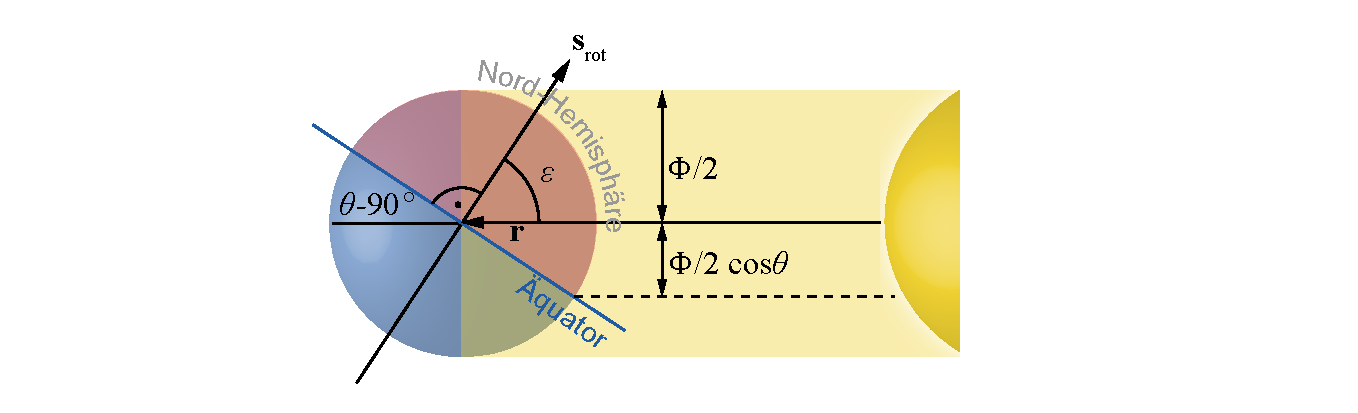
\includegraphics[width=\textwidth]{Erdbahn_im_Jahr_lsg3b.pdf}%
	\caption{Energieeintrag auf die Erde zur Sommersonnenwende}%
	\label{abb:hm_erdbahn_lsg_2}%
	\end{figure}
Der Sonnenlichtstrom $\Phi$ \anf{sieht} die Hemisph�ren unter einem Winkel $\theta$, der sich aus
	\begin{align*}
		\cos\theta(t) &= \frac{\vec{r}(\upsilon)\,\vec{s}_{\text{rot},\earth}}{\abs{\vec{r}(\upsilon)\,\vec{s}_{\text{rot},\earth}}} \nonumber\\
		              &= \lk \begin{matrix} \cos\upsilon(t) \\ \sin\upsilon(t) \\ 0 \end{matrix} \rk\,\lk \begin{matrix} \sin\epsilon \cos\alpha \\ \sin\epsilon\sin\alpha \\ \cos\epsilon \end{matrix} \rk  \\
									&= \sin\epsilon \lek \cos\alpha\cos\upsilon(t) + \sin\alpha\sin\upsilon(t)\rek \nonumber\\
									&= \sin\epsilon\,\cos\lek\upsilon(t)-\alpha\rek ~~ \nonumber
	\end{align*}
ergibt.
Die Sonneneinstrahlung trifft also je nach Jahreszeit auf unterschiedlich gro�e Teilfl�chen der jeweiligen Hemisph�re, der \anf{homogene} Strahlungsstrom verteilt $\Phi$ sich (wie im Bild zur Sommersonnenwende dargestellt) im Nordsommer auf die die Nord-Hemisph�re nach $(1\!+\!\cos\theta)/2$ und auf die S�d-Hemisph�re nach $(1\!-\!\cos\theta)/2$.
Wir berechnen jetzt den Energieeintrag pro "`Halbjahr"' und Hemisph�re und erhalten:
	\begin{align}
		H_\text{N,Sommer}&= C_\text{H}\,\frac{1}{\sqrt{a(1-e^2)}} \int\limits_{\alpha+\pi/2}^{\alpha+3\pi/2} \frac{\lek 1 + \sin\epsilon\cos(\upsilon-\alpha)\rek}{2}\, \D\upsilon \nonumber\\
		&= \frac{1}{2}\,C_\text{H}\,\frac{1}{\sqrt{a(1-e^2)}} \lek \pi-\sin\epsilon\sin(\upsilon-\alpha)\rek_{\alpha+\pi/2}^{\alpha+3\pi/2} \nonumber\\
		&= \frac{1}{2}\,C_\text{H}\,\frac{1}{\sqrt{a(1-e^2)}} (\pi+2\sin\epsilon) ~~.\label{eq:hm_erdbahn_lsg_10}
	\end{align}
	Eine analoge Beziehung erh�lt man f�r den Winter mit 
		\[H_\text{N,Winter} = \frac{C_\text{H}}{2}\,\frac{1}{\sqrt{a(1-e^2)}}\,(\pi-2\sin\epsilon) ~~,
	\]
woraus folgt:
\begin{equation}
\frac{\Delta H_\text{N}}{H_\text{ges}} = \frac{H_\text{N,Sommer} - H_\text{N,Winter}}{H_\text{ges}} = \frac{2\sin\epsilon}{\pi} ~~.\label{eq:hm_erdbahn_lsg_11}
\end{equation}
	
	Mit \eqref{eq:hm_erdbahn_lsg_10} und \eqref{eq:hm_erdbahn_lsg_6} k�nnen wir den durchschnittlichen Energieeintrag pro Zeit (also die empfangene Strahlungsleistung) in der n�rdlichen Hemisph�re f�r das Sommerhalbjahr berechnen:
	\begin{align}
		\frac{H_\text{N,Sommer}}{T_\text{Sommer}} &= P_\text{N,Sommer} \nonumber\\
		&= \frac{C_\text{H}\sqrt{\mu_\text{G}}(\pi+2\sin\epsilon)}{2\sqrt{a(1-e^2)}\, a^{3/2} \lek \pi+4e\cos\alpha-\frac{2e^3}{3}\cos(3\alpha)\rek} \nonumber\\
		&= \frac{P_\text{\astrosun}}{2}\,\lk\frac{R_\text{\earth}^2\sqrt{\mu_\text{G}}}{4\sqrt{\mu_\text{G}}\,a^2 \sqrt{1-e^2}}\rk \,\lk\frac{\pi+2\sin\epsilon}{\pi+4e\cos\alpha-\underbrace{\killA{\frac{2}{3}e^3\cos(3\alpha)}}_{\approx 0}}\rk \nonumber\\
		&\approx \frac{P_\text{\astrosun}}{8}\,\lk\frac{R_\text{\earth}^2}{a^2 \sqrt{1-e^2}}\rk \,\lk\frac{\pi+2\sin\epsilon}{\pi+4e\cos\alpha}\rk ~~.\label{eq:hm_erdbahn_lsg_12}
	\end{align}
	Wir k�nnen uns nun die tats�chlichen Werte und deren zeitliche Entwicklung anschauen.
        Wir finden dazu in den Tabellen \ref{tab:hm_bahnparameter} und \ref{tab:hm_zeitl_aenderung_bahnparameter_lin}
	\begin{align*}
		e &= 0.016709 - 3804\cdot 10^{-8}\,t ~~, \\
		\epsilon &= 23.4392911\degree + 46.8150''\,t =  23.4392911\degree + \frac{46.8150\degree}{3600} \,t ~~.
	\end{align*}
	Hier wird $t$ in Julianischen Jahrhunderten seit $J\,2000$ angegeben.
        F�r $\alpha$ k�nnen wir vereinfachend eine gleichm��ige Perihelpr�zession annehmen:
	\begin{equation*}
	\alpha(t) = \alpha_0 + 1.7192\degree \,t \approx -12.5\degree + 1.7192\degree \,t 
	\end{equation*}
	wobei wir die $1.7192\degree$ bereits als Ergebnis der Perihelverschiebung bzw. der unterschiedlichen L�ngen der tropischen und anomalistischen Jahre kennengelernt hatten.
	
	\begin{figure}[H]
	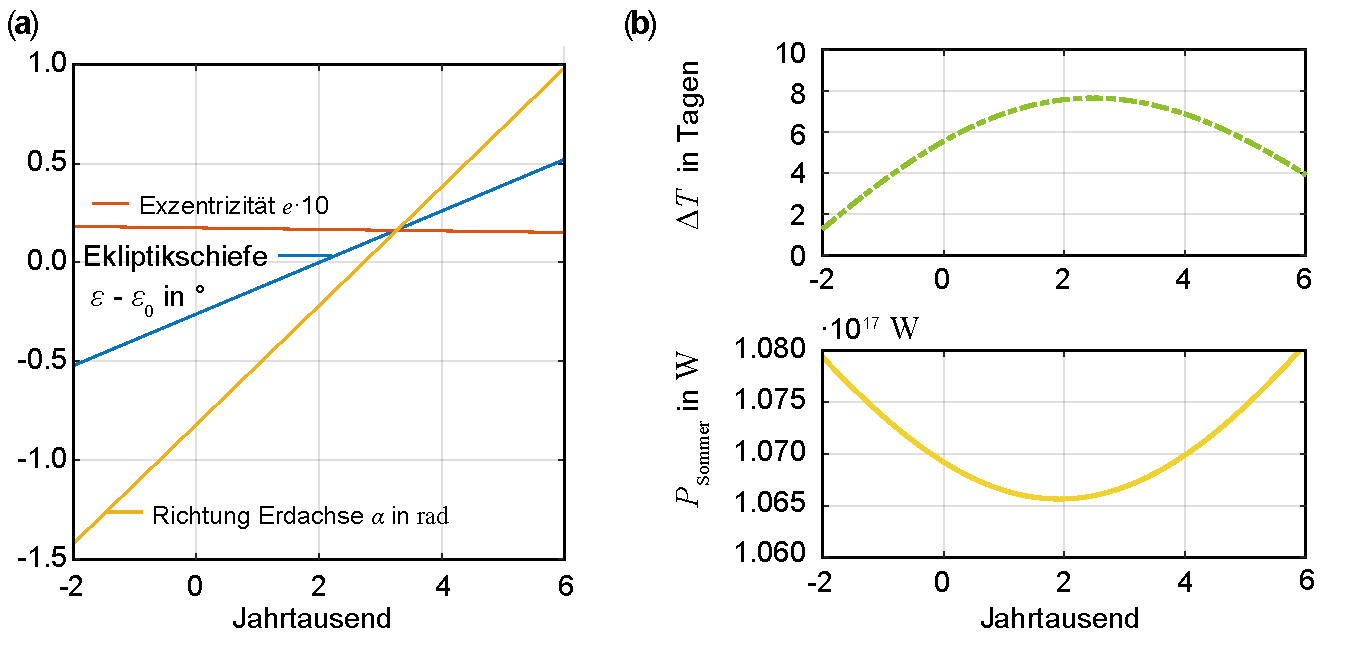
\includegraphics[width=\textwidth]{Erdbahn_im_Jahr_lsg_low.pdf}%
	\caption{Ver�nderung der zeitlichen Dauer der Jahreszeiten.}%
	\label{abb:hm_erdbahn_lsg_3}%
	\end{figure}
	
	In der \figref{hm_erdbahn_lsg_3} finden wir die Ver�nderung der zeitlichen Dauer der Jahreszeiten und auch den sich ver�ndernden  Energieeintrag f�r die Nord-Hemisph�re.
        Wir erkennen, dass wir uns im Moment in einer Trendwende befinden.
        Unser Sommerhalbjahr wird k�rzer werden.
        Gleichzeitig wird der mittlere Energieeintrag pro Halbjahr steigen.
        F�r langfristige Klimaeffekte kann man aber die Formel f�r $e$, $\epsilon$ und $\alpha$ nur bedingt benutzen, sondern muss Parametergleichungen als Funktion von $t$ finden, die einen Zeitraum von mehreren 100000 Jahren beschreiben \cite{Embacher2009}.
\end{enumerate}
\medskip
\end{sol} 
\textcolor{blue} {$\rightarrow$ zur} \probref{hm_erdbahn_im_jahr}.\\
\noindent\rule[1ex]{\textwidth}{0.5pt} \newpage

%-----------------------------------------------------------------------------------------------------------

\begin{sol}{prob:hm_refrak_optik}\label{lsg:hm_refrak_optik} %�bung11
\textbf{Refraktion -- ein Ausflug in die Optik} \\ \\
Wir beginnen mit dem planparallelen Modell (\figref{hm_refr_kugelschale_copy}).

\begin{figure}[H]
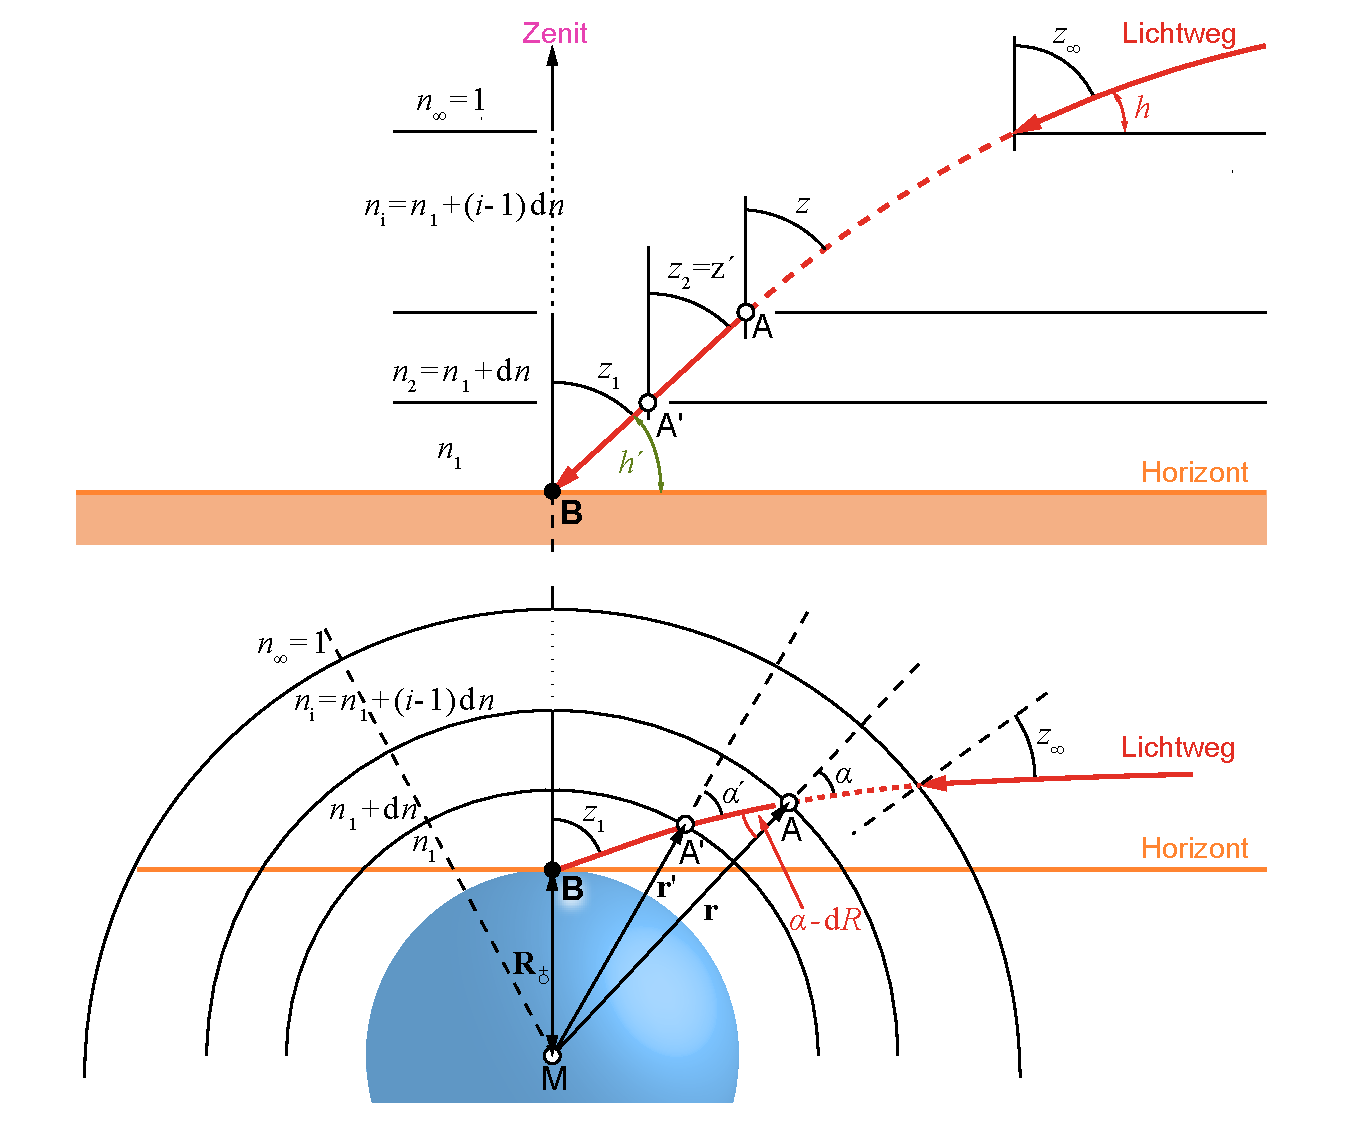
\includegraphics[width=\textwidth]{Refraktion0102.pdf}%
\caption[Planparalleles und Kugelschalen-Schichtenmodell.]{Planparalleles und Kugelschalen-Schichtenmodell zur Berechnung der Refraktion.
F�r die Winkel im $\bigtriangleup\mathrm{A}'\mathrm{MA}$ gilt: $\angle\mathrm{MA}'\mathrm{A}=180\degree-\alpha'$ und $\angle\mathrm{A}'\mathrm{MA}=\alpha-\D R$.}%
\label{abb:hm_refr_kugelschale_copy}%
\end{figure}
F�r die einzelnen Schichten mit unterschiedlichen Brechungsindizes $n_i$ k�nnen wir das Brechungsgesetz wie folgt aufschreiben:
\begin{equation}
n_1\,\sin z_1\,=\, n_2 \,\sin z_2\,=\,n_i\,\sin n_i\,=\,n_\infty\,\sin z_\infty ~~. \label{eq:hm_brechges_lsg12}
\end{equation}
Mit $z_\infty\!=\! [(90\degree - h]$,\, $z_1\!=\!90\degree - h'$,\, $n_\infty\!=\!1$ und der Definition $h\!=\!1h'-R$ folgt daraus
\begin{equation}
n_1\,\sin z_1 = \sin [(90\degree -h') + R] ~~. \label{eq:hm_R_lsg12a}
\end{equation}
Wie nehmen nun an, dass $R$ klein ist, was bei kleinen $z_\infty$ sicherlich gegeben ist und bekommen
\begin{align}
	n_1\,\sin z_1 &= \sin(90\degree - h') \, \cos R + \sin R \cos(90\degree - h')\, \nonumber \\
								& \approx \sin(90\degree - h') + R \cos(90\degree - h') = \sin z_1 + R \cos z_1 \nonumber \\
	\rightarrow ~~~~R &= (n_1 - 1)\,\tan z_1 ~~.  \label{eq:hm_R_lsg12b}
\end{align}
Die Refraktion\footnote{Ungl�cklicherweise bezeichnet man die Refraktion mit $R$, was oft zu Verwechslungen mit Radien und Abmessungen f�hrt. Da in der Literatur und insbesondere in Tabellen aber $R$ benutzt wird, halten wir uns ebenfalls an die Konvention.} $R$ ist also gegeben durch die im Allgemeinen unbekannte Brechzahl am Boden.
Man kann f�r Normalbedingungen und ein ideales Gas annehmen, dass die Brechzahl gem�� folgender Beziehung von der Dichte $\rho_\text{L}$ abh�ngt:
\begin{equation}
\frac{n^2-1}{n^2+2} \propto \rho_\text{L} = \frac{\bar{m}_\text{L} p_\text{L}}{R_0\,T} \label{eq:hm_brechzahl_von_dichte_lsg12}~~,
\end{equation}
worin $p_\text{L}$ der Luftdruck, $R_0\!=\! 8.31\!\cdot\! 10^3\:\text{J/(kmol\,K)}$ die Gaskonstante und $T$ die Temperatur ist.
Wir nehmen Normalbedingungen an, also $p_0\!=\! 101.325\:$kPa und $T_0\!=\! 293\:$K.
$\bar{m}_\text{L}\!\approx\! 28.95\:$kg/kmol ist das mittlere Molek�lgewicht des idealen Gases.
Aus \eqref{eq:hm_brechzahl_von_dichte_lsg12} kann man f�r $n\!\approx\!1$ schreiben:
\begin{equation}
\frac{(n+1)(n-1)}{n^2+2} \approx \frac{2}{3}\,(n-1) \propto \rho_\text{L} ~~.\label{eq:hm_glg4_lsg12}
\end{equation}
Setzt man \eqref{eq:hm_brechzahl_von_dichte_lsg12} und \eqref{eq:hm_glg4_lsg12} f�r verschiedene Temperaturen und Dr�cke ins Verh�ltnis, erh�lt man
\begin{align}
	n_1 - 1 &\approx (n_{10} - 1)\,\frac{p}{p_0}\,\frac{T_0}{T} = (n_{10} - 1)\, 2.6947\,\frac{p}{T} \nonumber\\
\Rightarrow R &= (n_{10}-1)\, 2.6947\,\frac{p}{T}\,\tan(90\degree - h') ~~.\label{eq:hm_glg5_lsg12}
\end{align}
Diese Beziehung f�r $R$ gilt nur f�r kleine $z_1$ oder gr��ere H�hen $h$, also nicht f�r den Fall der Berechnung des Sonnenaufgangs.
Wir wollen deshalb die Refraktion $R$ nach dem Kugelschalenmodell in \figref{hm_refr_kugelschale_copy}b berechnen und k�nnen hier das Brechungsgesetz f�r verschiedene Schichten wie folgt aufschreiben (Man betrachte Punkt A in \figref{hm_refr_kugelschale_copy}b.):
\begin{equation}
(n+ \D n)\,\sin(\alpha-\D R) = n\,\sin\alpha ~~. \label{eq:hm_glg6_lsg12}
\end{equation}
Wiederum ist $\D R$ eine kleine Gr��e, so dass aus \eqref{eq:hm_glg6_lsg12} gleich folgt:
\begin{align}
	(n+\D n)[\sin\alpha \underbrace{\cos(\D R)}_{\approx 1} - \cos\alpha \underbrace{\sin(\D R)}_{=\D R}] &= n\,\sin\alpha \nonumber\\
	\killA{n\,\sin\alpha} + \D n\,\sin\alpha - n\,\cos\alpha\,\D R &= \killA{n\,\sin\alpha} \nonumber\\
	\Rightarrow \D R &= \frac{\D n}{n}\,\tan\alpha ~~. \label{eq:hm_glg7_lsg12}
\end{align}
Wir ersetzen nun $\tan\alpha$ und benutzen dazu den Sinussatz im Dreieck $\bigtriangleup\text{MA'A}$:
\begin{equation}
\frac{\sin\alpha'}{r} = \frac{\sin(\alpha-\D R)}{r'} ~~. \label{eq:hm_glg8_lsg12}
\end{equation}
Kombinieren wir \eqref{eq:hm_glg6_lsg12} und \eqref{eq:hm_glg8_lsg12} erhalten wir durch Einsetzen von $\sin(\alpha-\D R)$
\begin{equation*}
r'(n + \D n)\,\sin\alpha' = rn\,\sin\alpha ~~.
\end{equation*}
Diese Beziehung gilt analog zu \eqref{eq:hm_brechges_lsg12} f�r alle Schichten.
Deshalb k�nnen wir schreiben:
\begin{equation}
rn(r)\,\sin\alpha = R_\text{\earth} n_1\,\sin z_1
\label{eq:hm_glg9_lsg12}~~.
\end{equation}
Wir benutzen jetzt noch die trigonometrische Beziehung $\tan\alpha = \sin\alpha/\sqrt{1-\sin^2\alpha}$ und k�nnen damit \eqref{eq:hm_glg7_lsg12} umformen zu
\begin{equation}
R(z_1) = \int \D R = \int\limits_{n=1}^{n=n_1} \frac{1}{n}\,\frac{A \sin z_1}{\sqrt{1-A^2\sin^2 z_1}} \,\D n \label{eq:hm_glg10_lsg12}
\end{equation}
mit 
	\[	A(n)\!=\frac{\!R_\text{\earth} n_1}{r n(r)} ~. 
	\]
Die Gleichung \eqref{eq:hm_glg10_lsg12} nennt man das Refraktionsintegral.\index{Refraktionsintegral}
Will man dieses auswerten, so muss man Annahmen f�r $n(r)$ bzw. $\rho_\text{L}(r)$ machen, die wiederum von $T(r)$ und $p(r)$ abh�ngen.
Im Allgemeinen wird das Integral numerisch gel�st.
Man kann dann auch beliebige Schichtmodelle annehmen und $ R$ �ber
\begin{equation*}
R = \sum_{i=1}^{i=N} \tan\alpha_i\,\lk\frac{n_{i+1} - n_i}{n_i}\rk
\end{equation*}
mit $\alpha_1\!=\! z_1\!=\! z_\text{schein}$ berechnen. 
Interessant ist noch, dass bereits Newton auf Basis seiner Korpuskulartheorie des Lichtes die Berechnung der Refraktion vornahm und diese als eine der kompliziertesten Aufgaben seines Lebens bezeichnete \cite{Nauenberg2017}. Er berechnete die Trajektorie des Lichtteilchens, welches durch die Brechung unter einer \emph{Zentralkraft} der Form
\begin{equation*}
\vec{F} = n\,\frac{\D n}{\D r} \frac{\vec{r}}{r}
\end{equation*}
steht.
Mit den Methoden, die wir in \kapitel{hm_bewegungsgl} dargestellt haben, insbesondere die Benutzung der Drehimpulserhaltung, kann man die Trajektorie des Teilchens als 
\begin{equation*}
z(r) = \bigintss\limits_{r_1 = R_\text{\earth}}^{r} \frac{\sin z_1}{r' \sqrt{\lk \frac{n(r') r'}{n_1 R_\text{\earth}} \rk^2 - \sin^2 z_1}} \D r'
\end{equation*}
und die Refraktion als
\begin{equation*}
R(z_1) = z_1 - z(r\rightarrow\infty) \equiv R(z') = z' - z 
\end{equation*}
schreiben \cite{Nauenberg2017}.
Wir wollen noch die Formulierung des Refraktionsintegrals f�r eine einfache Abh�ngigkeit der Brechungsindizes von der H�he angeben, der durch eine exponentielle Abnahme der Dichte nach
\begin{align*}
	\rho(r') = \rho(R_\text{\earth})\,\E^{-h/H} = \rho_0\,\E^{-h/H} ~~\text{mit} ~~ h = r - R_\text{\earth}
\end{align*}
nach folgender Formel 
\begin{align*}
	n(r') -1 = \kappa \,\frac{\rho(r')}{\rho(R_\text{\earth})} 
\end{align*}
gegeben ist, worin $\kappa$ und $H$ Konstanten der Erdatmosph�re sind.
In das Refraktionsintegral \eqref{eq:hm_glg10_lsg12} eingesetzt, ergibt das 
\begin{equation}
R(z_1) = \kappa \bigintss\limits_{0}^{\infty} \frac{\E^{-x}\,\sin z_1}{\lk 1+\kappa \E^{-x}\rk\,\sqrt{\lek \lk 1+\kappa \E^{-x} \rk \lk 1 + \frac{Hx}{R_\text{\earth}} \rk / \lk 1+\kappa\rk \rek^2 - \sin^2 z_1}} \:\D x ~~, \label{lsg:hm_refraktionsintegral2}
\end{equation}
welches wir in \mlhmref{Refraktion.m} f�r verschiedene Parameter $\kappa, H$ ausgewertet haben.
Als Parameter f�r einen relativ guten Fit an die Formel \eqref{eq:hm_Normalrefraktion1} haben wir aus der ISA-Tabelle \cite{ISA1976} die Werte $\kappa\!=\! 0.000316$ und $H\!=\! 9.87 $ km gew�hlt.

\begin{figure}[H]
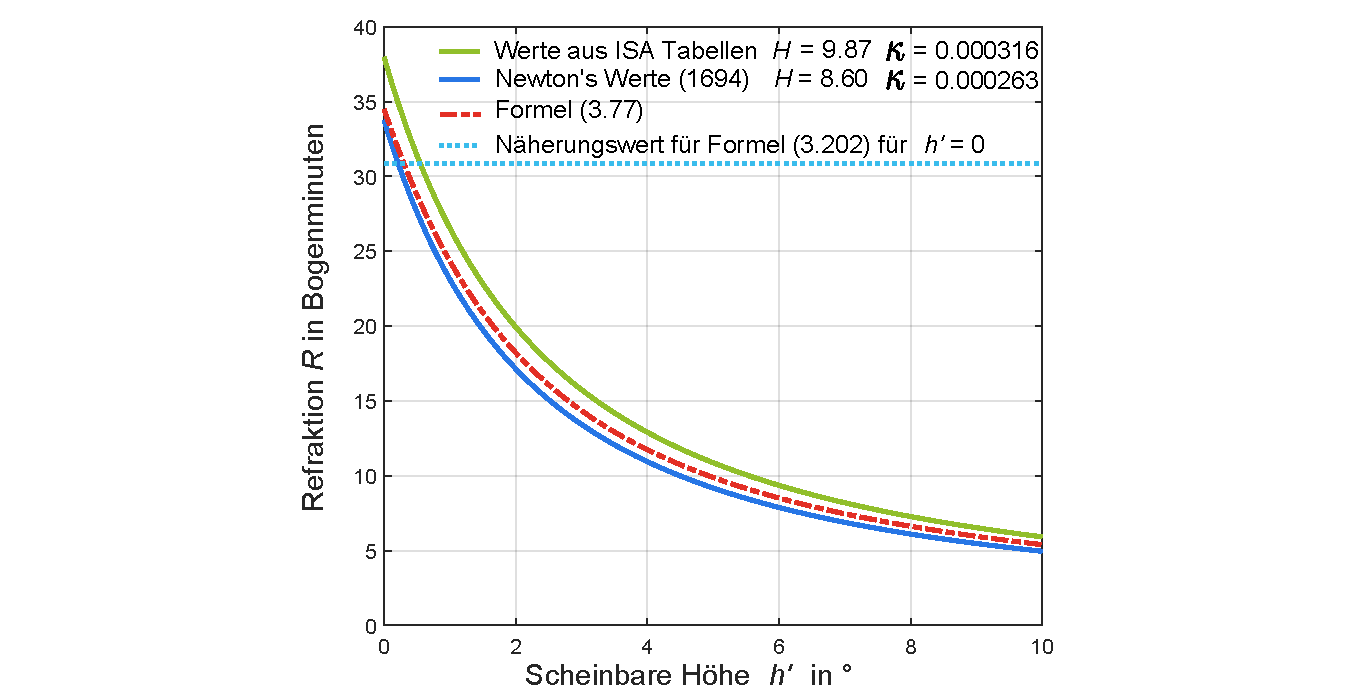
\includegraphics[width= \textwidth]{Refraktion12.pdf}%
\caption[Berechnete Refraktionskurven nach dem Kugelschalen-Schichtenmodell.]{Berechnete Refraktionskurven nach dem Kugelschalen-Schichtenmodell \eqref{lsg:hm_refraktionsintegral2} und Vergleich mit \eqref{eq:hm_relations2} sowie den Berechnungen von Newton \cite{Nauenberg2017}.}%
\label{abb:hm_Refraktion12}%
\end{figure}
\medskip \end{sol}
\textcolor{blue} {$\rightarrow$ zur} \probref{hm_refrak_optik}.\\
\noindent\rule[1ex]{\textwidth}{0.5pt} \newpage


\begin{sol}{prob:hm_abflachung_sonne} \label{lsg:hm_abflachung_sonne} %�bung12
\textbf{Abflachung der Sonne beim Untergang} \\

\begin{figure}[H]
\includegraphics[width=1.0\textwidth]{AbflachungSonne.pdf}%
\caption[Berechnung der Abflachung der Sonne bei Sonnenuntergang.]{Berechnete Form und H�he der Sonne mit (links) und ohne Refraktion (rechts). Bildmitte: Aufnahme Sonnenuntergang auf Hawaii (Bernd Geh am 10.11.2016 um 17:42:32) und dazu berechnete Form und Position.}%
\label{abb:hm_AbflachungSonne}%
\end{figure}

Wir benutzen zur L�sung die Refraktionsformel Formel \eqref{eq:hm_Normalrefraktion2}.
im Bild links sind die \anf{abgeflachten} Sonnen in der scheinbaren H�he zu sehen und rechts im Bild in gleicher Farbumrandung in astrometrische H�he und in der nicht durch Refraktion beeinflussten Form der \anf{Sonnenscheibe}.
In der Mitte ist ein auf Hawaii von Bernd Geh aufgenommenes Bild der untergehenden Sonne gefittet.
Wir verweisen auf \mlhmref{AbflachungSonne.m} und bedanken uns bei Bernd Geh (\href{http://www.bgeh-photography.com/Home.html}{http://www.bgeh-photography.com/Home.html}) f�r die Bereitstellung des Bildes und die Anregungen zur �bung.\\
\medskip \end{sol}
\textcolor{blue} {$\rightarrow$ zur} \probref{hm_abflachung_sonne}.\\
\noindent\rule[1ex]{\textwidth}{0.5pt} \newpage

\begin{sol}{prob:hm_tageslauf_sonne} \label{lsg:hm_tageslauf_sonne} %�bung13
\textbf{Tageslauf der Sonne} \\ \\
Wir verweisen auf das \mscr~\mlhmref{TageslaufSonne.m}. \\
\medskip \end{sol}
\textcolor{blue} {$\rightarrow$ zur} \probref{hm_tageslauf_sonne}.\\
\noindent\rule[1ex]{\textwidth}{0.5pt} \newpage

\begin{sol}{prob:hm_sonnenaufg_nyc}\label{lsg:hm_sonnenaufg_nyc} %�bung14
\textbf{Sonnenaufgang in New York City} \\ \\
Basierend auf \figref{hm_nyc_lsg} berechnen wir zun�chst aus der geographischen Breite $\varphi= 40.7\degree$ von New York City (NYC) den Radius des Erdellipsoids an dieser Stelle \cite{Meeus1998}:
\begin{align*}
	r_\text{NYC} &= \lek 0.9983271 + 0.0016764 \cos(2\varphi) - 0.0000035 \cos(4\varphi)\rek\, 6378137\:\text{m} \\
	&= 6369087\:\text{m}~.\\
\end{align*}

\begin{figure}[H]

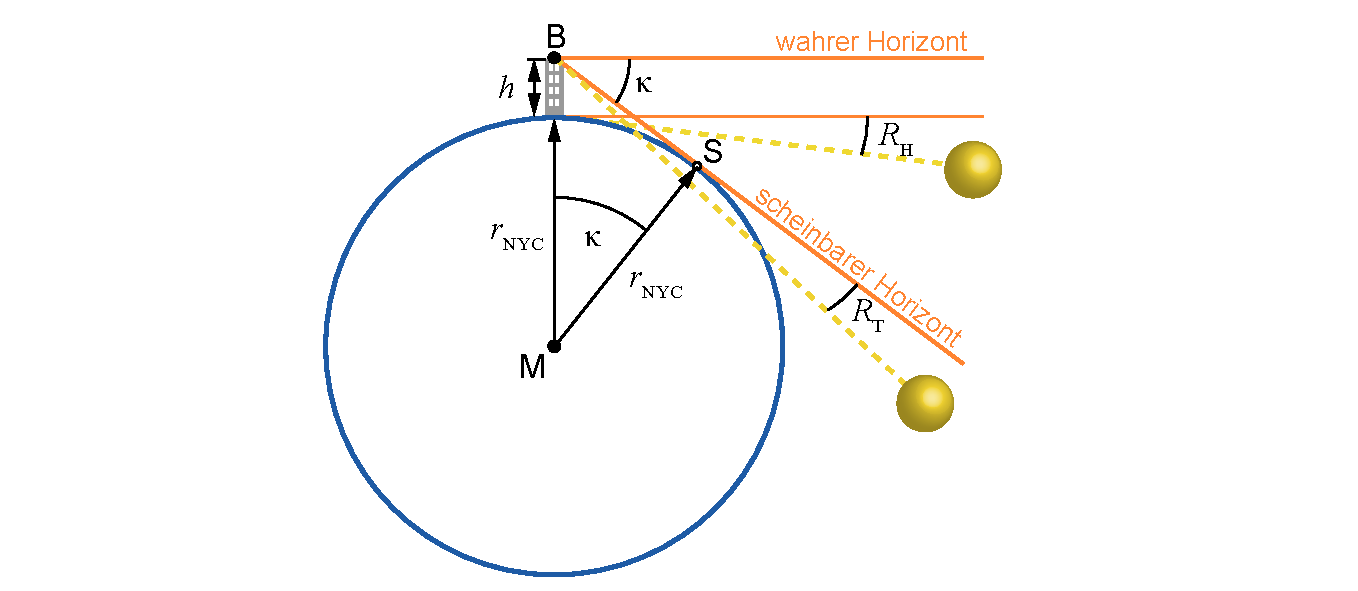
\includegraphics[width=\textwidth]{SonnenaufgangNYC.pdf}%
\caption{Geometrie zum Sonnenaufgang in New York City}%
\label{abb:hm_nyc_lsg}%
\end{figure}

Die H�he $h$ des One World Trade Centers betr�gt $531\:$m.
Daraus ergibt sich der Winkel $\kappa$ aus \figref{hm_nyc_lsg} �ber.
Es gilt weiterhin
\begin{align*}
	(r_\text{NYC} + h)^2 &= \overline{\text{BS}}^2 + r_\text{NYC}^2 \\
	\rightarrow \overline{\text{BS}} &\approx \sqrt{2\,h\,r_\text{NYC}} ~~\text{f�r}~~h\ll r_\text{NYC}~~.
\end{align*}
Es ergibt sich f�r kleine Winkel $\kappa$:
\begin{equation}
\tan \kappa \approx \sin \kappa = \frac{\overline{\text{BS}}}{r_\text{NYC}} = \sqrt{\frac{2h}{r_\text{NYC}}}~~,
\end{equation}
woraus $\kappa = 0.73981$ folgt.
Wir sehen ferner aus der Abbildung, dass ohne Ber�cksichtigung der Refraktion, der Sonnenaufgang um eine bestimmte Zeitdauer $\Delta t$ fr�her stattfindet.
$\Delta t$ entspricht der Zeit, die die Sonne br�uchte, um die H�he $h$ zu durchlaufen.
Wenn wir noch ber�cksichtigen, dass die Refraktion $R_\text{T}$ etwas gr��er ist als $R_\text{H}$,\footnote{Das Licht durchl�uft dichtere Luftschichten deutlich langsamer.} dann k�nnen wir f�r die Tagbogenverl�ngerung mit \eqref{eq:hm_tagbogverl} und $\delta\!= \epsilon\!\,$ folgendes aufschreiben:
\begin{align*}
	\Delta\tau_\text{B,H} &= -\frac{h_\text{r,H}}{\sqrt{\cos^2\delta - \sin^2\varphi}} = \frac{-16' - R_\text{H}}{\sqrt{\cos^2\delta - \sin^2\varphi}} ~~,\\
	\Delta \tau_\text{B,T} &= -\frac{h_\text{r,T}}{\sqrt{\cos^2\delta - \sin^2\varphi}} = \frac{-\kappa-16' - R_\text{T}}{\sqrt{\cos^2\delta - \sin^2\varphi}} ~~.
\end{align*}
Aus \eqref{eq:hm_Normalrefraktion1} finden wir zun�chst $R_\text{H} \!=\!R(0)\!\approx\! 34'$ und $R_\text{T} \!=\!R(-\kappa)\!\approx\! 45'$ und somit
\begin{align}
	\Delta t &= \Delta\tau_\text{B,1} - \Delta\tau_\text{B,0} \\
	        &= -\frac{(R_\text{T} - R_\text{H})+\kappa}{\sqrt{\cos^2 \delta - \sin^2 \varphi}} \\
					&\approx 5\:\text{min} ~ 45\:\text{s}~~.
\end{align}
Der Beobachter auf dem One World Trade Center sieht also die Sonne fast $6\:$min fr�her als jener auf Ellis Island.
Es lohnt sich also seinen Morgenkaffee auf dem One WTC zu trinken.\\
\medskip \end{sol}
\textcolor{blue} {$\rightarrow$ zur} \probref{hm_sonnenaufg_nyc}.\\
\noindent\rule[1ex]{\textwidth}{0.5pt} \newpage


%-----------------------------------------------------------------------------------------------------------

\begin{sol}{prob:hm_analytic_sunrise}\label{lsg:hm_analytic_sunrise} %�bung15
\textbf{Analytische Formel f�r den Sonnenaufgang und Sonnenuntergang} \\ \\
Wir folgen hier der Darstellung in \cite{Reinsch2003} und starten von der Beziehung f�r die astronomische H�he als Funktion des Stundenwinkels \eqref{eq:hm_Alt-Az-Koord}
\begin{equation*}
\sin h = \cos\delta \cos\tau \cos\varphi + \sin\delta \sin\varphi ~~.
\end{equation*}
Wir ersetzen die Deklination $\delta$ durch die geozentrisch-ekliptikale Koordinate $\lambda$ nach \eqref{eq:hm_drehung_x_achse_linear2} und erhalten mit $\beta\!=\!0$ und $\tau\!=\!\Theta-\alpha$ gem�� \eqref{eq:hm_std_winkel_tau} f�r die Sonne
\begin{align}
\sin h =&\, \underbrace{\cos\delta \cos\alpha}_{=\cos\lambda} \cos\Theta \cos\varphi + \underbrace{\cos\delta \sin\alpha}_{\sin\lambda \cos\epsilon} \sin\Theta \cos\varphi\, + \underbrace{\sin\delta}_{\sin\lambda \sin\epsilon} \sin\varphi \nonumber\\
			 =&\, \cos\lambda \cos\Theta \cos\varphi + \sin\lambda\cos\epsilon\sin\Theta\cos\varphi + \underbrace{\sin\lambda \sin\epsilon \sin\varphi}_{\equiv\text{T}_\text{II}} ~~. \label{eq:hm_sa_su_lsg1}
\end{align}
Die Aufgabe besteht nun darin, $\Theta(h\!=\!0)$ bzw. $\tau(h\!=\!0)$ f�r die Tage eines Jahres zu bestimmen.
Wir wollen dabei vereinfachend f�r die Sternzeit $\Theta$ annehmen, dass
\begin{equation}
\Theta = \frac{2\pi}{\text{d}_\diamond}\, t = \frac{2\pi}{86164\:\text{s}}\, t ~~. \label{eq:hm_sa_su_lsg2a}
\end{equation}
F�r die Weltzeit UT schreiben wir 
\begin{equation}
\hat{\Theta} = \frac{2\pi}{\text{d}_\text{\astrosun}}\, t = \frac{2\pi}{86400\:\text{s}}\, t ~~. \label{eq:hm_sa_su_lsg2b}
\end{equation}
Da wir besser die Uhrzeit und nicht die Sternzeit des Sonnenaufgangs bestimmen wollen, formen wir dies um zu
\begin{equation*}
\Delta (t) = \Theta - \hat{\Theta} ~~\text{bzw.}~~ \Theta = \hat{\Theta}+\Delta
\end{equation*}
und setzen diese Beziehung in \eqref{eq:hm_sa_su_lsg1} ein.
$\Delta (t)$ beschreibt im Prinzip das \anf{Auseinanderlaufen} von Sternzeit und Weltzeit, was exakt durch \eqref{eq:hm_UT_3} gegeben ist.
F�r unsere Absch�tzung des Sonnenaufgangs gen�gt aber der einfache Ansatz nach \eqref{eq:hm_sa_su_lsg2a} und \eqref{eq:hm_sa_su_lsg2b}.
Wir bekommen also
\begin{equation*}
\sin h = \underbrace{\cos\lambda \cos(\hat{\Theta}+\Delta) \cos\varphi + \sin\lambda \cos\epsilon \sin(\hat{\Theta}+\Delta) \cos\varphi}_{\equiv \text{T}_\text{I} = X \cos(\hat{\Theta}+\xi)\cos\varphi} + \text{T}_\text{II} ~~,
\end{equation*}
was eine algebraische Umformung unter Nutzung der Additionstheoreme ist. Mit den Termen
\begin{equation*}
X = \sqrt{\lk \cos\epsilon \sin\lambda \sin\Delta + \cos\lambda \cos\Delta \rk^2 + \lk \cos\epsilon \sin\lambda \cos\Delta - \cos\lambda \sin\Delta\rk^2}
\end{equation*}
und
\begin{equation*}
\xi = -\arctan \lk \frac{\cos\epsilon \sin\lambda \cos\Delta - \cos\lambda \sin\Delta}{\cos\epsilon \sin\lambda \sin\Delta + \cos\lambda \cos\Delta} \rk
\end{equation*}
erhalten wir schlie�lich
\begin{equation}
\sin h = \text{T}_\text{I} + \text{T}_\text{II} = X \cos (\hat{\Theta}+\xi) \cos\varphi + \sin\lambda \sin\epsilon \sin\varphi ~~.\label{eq:hm_sa_su_lsg3}
\end{equation}
Wir m�ssen jetzt eigentlich nur noch \eqref{eq:hm_sa_su_lsg3} nach $\hat{\Theta}$ f�r $h\!=\!0$ l�sen und machen hierzu die folgende N�herungen:
\begin{itemize}
	\item Vernachl�ssigung der Refraktion,
	\item Annahme, dass die ekliptikale L�nge $\lambda$ und $\Delta$ f�r die Dauer eines Tages konstant sind.
\end{itemize}
Wenn man mit \eqref{eq:hm_sa_su_lsg2a} mod $24\:$h bzw. mod $\pi$ nimmt und $h\!=\!0$ aus \eqref{eq:hm_sa_su_lsg3} benutzt, folgt daraus
\begin{equation}
\hat{\Theta}_\text{A,U} = \pm \arccos \lk - \frac{\sin\lambda \sin\epsilon \tan\varphi}{X} \rk - \xi ~~. \label{eq:hm_sa_su_lsg4}
\end{equation}
Dabei gilt das Minuszeichen f�r den Sonnenaufgang und das Pluszeichen f�r den Sonnenuntergang.
Laut unserer Definition der ekliptikalen L�nge ist ja am Fr�hlingspunkt $\lambda\!=\!0$ und die Uhren sind synchron  $\hat{\Theta} = \Theta$.
Es folgt demnach
\begin{equation*}
\hat{\Theta}_\text{A,U}(\vernal) = \underbrace{\tan \Delta(\vernal)}_{0} \pm \arccos (0) = \pm \frac{\pi}{2} = \pm 6\:\text{h} 
\end{equation*}
und damit der Sonnenaufgang als $\text{SA}\!=\!12\:\text{h}-\hat{\Theta}(\vernal) =$ 06:00h UT.
Wir haben mit \eqref{eq:hm_sa_su_lsg4} eine relativ �bersichtliche Formel f�r die Berechnung der Sonnenaufg�nge und Sonnenunterg�nge gefunden. 

\begin{figure}[H]
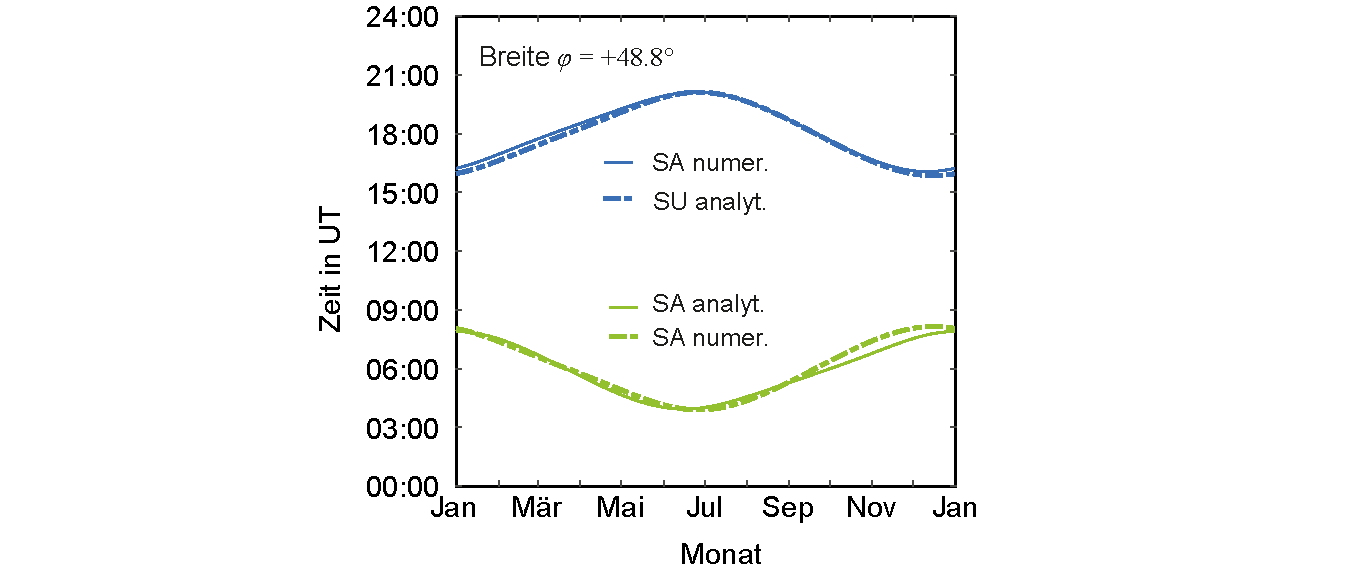
\includegraphics[width=\columnwidth]{Sunrise_lsg.pdf}%
\caption[Analytische und numerische L�sung Sonnenauf- und Sonnenuntergang.]{Analytische und numerische L�sung des Sonnenaufgangs und Sonnenuntergangs.}%
\label{abb:hm_sunrise_lsg}%
\end{figure}

Als Parameter f�r die N�herungsl�sung ben�tigen wir die L�nge des Sternen- und Sonnentags in Sekunden, die geographische Breite $\varphi$, die Ekliptikschiefe $\epsilon$ und die ekliptikale L�nge $\lambda$.
Letztere beschaffen wir uns wieder aus der Mittelpunktsgleichung \eqref{eq:hm_ekl_laenge_bogenmass}, womit in \eqref{eq:hm_sa_su_lsg4} wieder beide Effekte (Ekliptikschiefe und Elliptizit�t der Bahn) ber�cksichtigt worden sind.
In \figref{hm_sunrise_lsg} vergleichen wir die L�sung in \eqref{eq:hm_sa_su_lsg4} mit der numerischen L�sung, die �bereinstimmung ist relativ gut.
Es sei erw�hnt, dass die N�herungsformeln nicht gelten, wenn wir in den Bereich $\abs{\varphi}\!>\!+(90\degree\!-\!\epsilon)$ kommen.
Die analytische Formel wird dar�ber hinaus auch wegen des Verhaltens der $\arccos$-Funktion bei kleinen Argumenten f�r $\abs{\varphi}\!\ll\! \epsilon$ ungenau.
\medskip \end{sol}
\textcolor{blue} {$\rightarrow$ zur} \probref{hm_analytic_sunrise}.\\
\noindent\rule[1ex]{\textwidth}{0.5pt} \newpage


%-----------------------------------------------------------------------------------------------------------

\begin{sol}{prob:hm_VertikalAnalemmaSonnenuhr} \label{lsg:hm_VertikalAnalemmaSonnenuhr} %\�bung16
\textbf{Konstruktion von Sonnenuhren} \\

Konstruktion einer vertikalen und einer analemmatischen Sonnenuhr:
\begin{figure}%
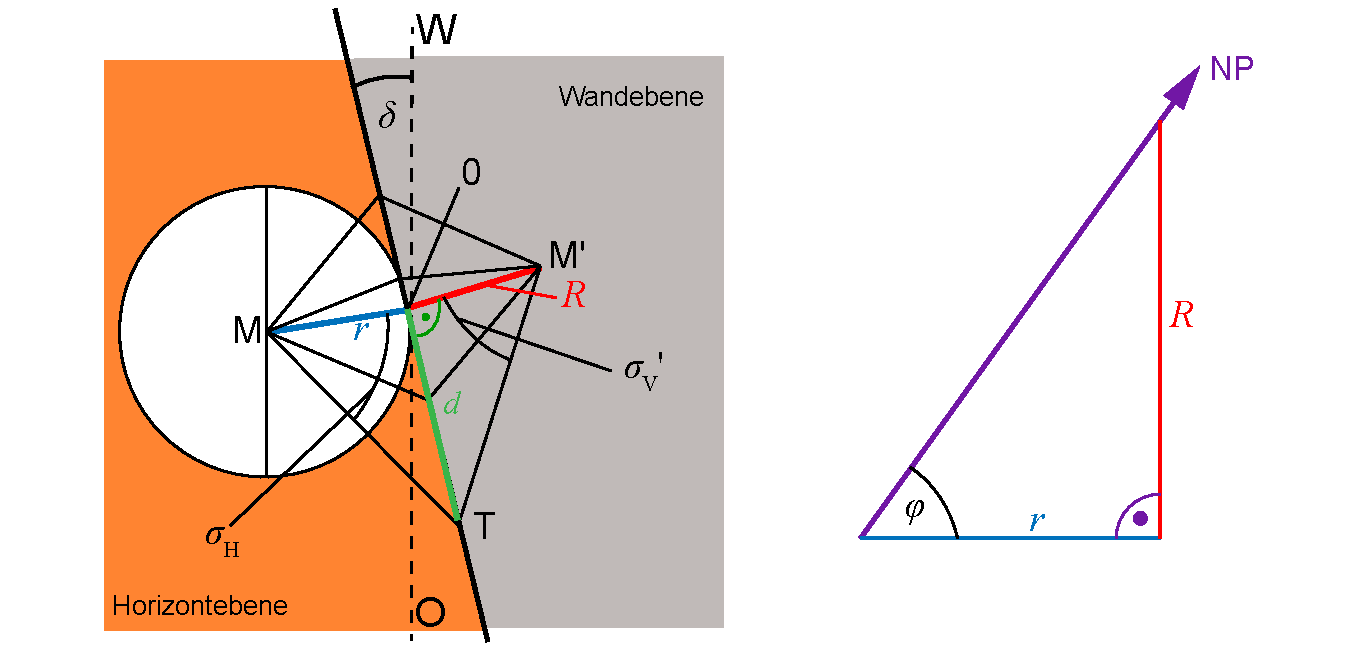
\includegraphics[width=\textwidth]{Sonnenuhr05.pdf}%
\caption[Ausf�hrung und Prinzip der Vertikal-Sonnenuhr.]{Ausf�hrung und Prinzip der Vertikal-Sonnenuhr bei  beliebiger Ausrichtung der Wand.}%
\label{abb:hm_sundial_lsg01}%
\end{figure}

\begin{enumerate}
 \item [a)]  

Wir betrachten zun�chst die Sonnenuhr, die an einer Hauswand angebracht ist, welche unter einem beliebigen Winkel $\delta$ zur Ost-West-Richtung steht.
Der Verdrehwinkel $\delta$ zur Wand sei negativ bei Ausrichtung SW-NO, wie im dargestellten Fall.
Aus \figref{hm_sundial_lsg01} lesen wir folgende Beziehungen ab:
    \begin{align}
        \tan\sigma_v{}' &= \frac{\overline{\text{0T}}}{R} = \frac{d}{R} \label{eq:hm_sundial_lsg01} \\
        \sphericalangle (\text{MT0}) &= 180\degree - (90\degree - \delta) - \sigma_\text{H} = 90\degree - (\sigma_\text{H} -\delta)\,. \label{eq:hm_sundial_lsg01a} 
    \end{align}
    Aus dem Sinussatz f�r das Dreieck $\Delta (\text{MT0})$ folgt:
    \begin{align}
        \frac{\sin\sigma_\text{H}}{d} = \frac{\sin \sphericalangle (\text{MT0})}{r} ~~~~\rightarrow ~~~~ d = r\,\frac{\sin\sigma_\text{H}}{\cos\lk \sigma_\text{H} - \delta \rk} \,. \label{eq:hm_sundial_lsg02}
    \end{align}
    Mit der Beziehung \eqref{eq:hm_sundial02} f�r die Radien $r$ und $R$ \,$ \tan\varphi = R/r$ und mit \eqref{eq:hm_sundial_lsg01} und \eqref{eq:hm_sundial_lsg02} folgt daraus:
    \begin{align}
        \tan\sigma_\text{V}{}' &= \frac{\sin\sigma_\text{H}}{\cos\lk \sigma_\text{H}- \delta\rk}\,\frac{1}{\tan\varphi} ~~~~ \text{mit} ~~~~ \sigma_\text{H} = \arctan \lk\sin\varphi\,\tan\sigma_\text{A} \rk \nonumber \\
				\rightarrow~\sigma_\text{V}{}' &= \arctan\lk \frac{\cos\varphi}{\cos\delta \cot\sigma_\text{A} + \sin\varphi \sin\delta}\rk	\,.
\label{eq:hm_sundial_lsg03}
    \end{align}
    F�r $\delta \to 0$ folgt daraus mit 
    \begin{align*}
        \tan\sigma_\text{V}{}' &= \frac{\sin\sigma_\text{H}}{\cos\sigma_\text{H}}\,\frac{1}{\tan \varphi} = \frac{\sin\varphi}{\tan\varphi}\,\tan\sigma_\text{A} = \cos\varphi\,\tan\sigma_\text{A} \\
    \end{align*}
    die Beziehung f�r die O-W ausgerichtete Wand.
    Die Lineatur f�r eine Sonnenuhr in Oberkochen ($\varphi = 48\degree$ N) und einer Wand die etwa ONO-WSW ausgerichtet ist ($\delta = -22.5\degree$) ist in \figref{hm_sundial_lsg02} zu sehen.\\

\begin{figure}%
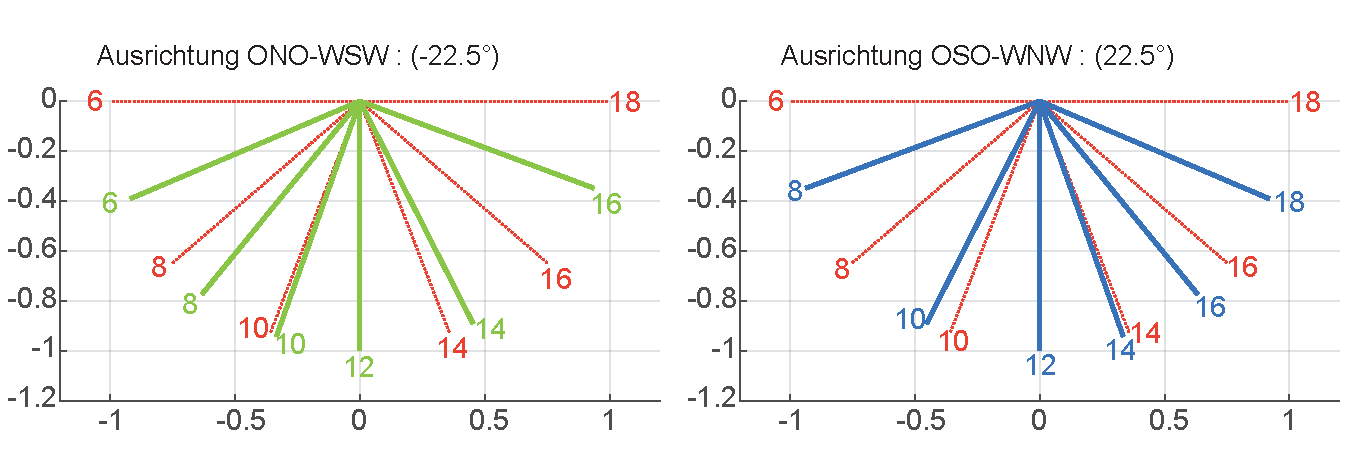
\includegraphics[width=\textwidth]{Wandsonnenuhr.pdf}%
\caption[Lineatur f�r eine Wandsonnenuhr in Oberkochen.]{Lineatur f�r eine Wandsonnenuhr in Oberkochen f�r verschiedene Ausrichtungen. Siehe \mlhmref{Wandsonnenuhr.m}} 
\label{abb:hm_sundial_lsg02}%
\end{figure}

\item [b)]

Nun wollen wir die Lineatur f�r eine analemmatischen Sonnenuhr in der Stadt G�rlitz (Breitengrad $\varphi = 51.2\degree$ und L�ngengrad $\lambda = 15\degree$) berechnen. 
Aus \eqref{eq:hm_sundial06} k�nnen wir die Abbildung $\vec{r}_n$ des Nodus aus der Sonnenrichtung $\vec{s}$ auf dem Ziffernblatt (welches in der Horizontalebene liegt) als Funktion des Datums und der Zeit, m.\,a.\,W.\ als Funktion des Sonnenstandes f�r eine bestimmte geographische Breite berechnen. \\
Wir k�nnen zur Berechnung nat�rlich vorteilhafter weise, die in \kap{hm_naeherungsformeln_sonne} berechneten Beziehungen f�r die H�he $h$ und das Azimut $\mathcal{A}$ der Sonne benutzen. Dann ergeben sich die Linien des Schatten des Nodus f�r einen bestimmten Tag eines Jahres $d_\text{fix}$ durch (wir nehmen die WSW, SSW und die Tag- und Nachtgleichen):
    \begin{align}
        \vec{r}_n (t) &= 
         \begin{pmatrix}
         \cos \lk h\lk t, d_\text{fix}\rk \rk \, \cos \lk \mathcal{A}\lk t,d_\text{fix} \rk\rk \\
         \cos \lk h\lk t, d_\text{fix}\rk \rk \, \sin \lk \mathcal{A}\lk t,d_\text{fix} \rk\rk \\
         0
         \end{pmatrix}\cdot
         \frac{H}{\sin h\lk t,d_\text{fix} \rk}\nonumber \\
          &= H\, 
         \begin{pmatrix}
             \cot\lk h\lk t,d_\text{fix}\rk\rk\,\cos\lk \mathcal{A}\lk t,d_\text{fix}\rk\rk\\
             \cot\lk h\lk t,d_\text{fix}\rk\rk\,\sin\lk \mathcal{A}\lk t,d_\text{fix}\rk\rk\\
             0
         \end{pmatrix} \,.  \label{eq:hm_lsgsundial11}
    \end{align}
    Analog ergibt sich f�r eine feste Uhrzeit $t_\text{fix}$ und die verschiedenen Tage $d$ des Jahres nat�rlich die Form des Analemma. 
    \begin{align}
        \vec{r}_n (d) = H\,
        \begin{pmatrix}
            \cot\lk h\lk t_\text{fix},d\rk \rk \, \cos\lk \mathcal{A}\lk t_\text{fix},d\rk \rk \\
            \cot\lk h\lk t_\text{fix},d\rk \rk \, \sin\lk \mathcal{A}\lk t_\text{fix},d\rk \rk \\
            0
        \end{pmatrix} \,.  \label{eq:hm_lsgsundial12}
    \end{align}
    $d$ steht hier f�r die Tage des Jahres. Die bei den Einzellineaturen nach \eqref{eq:hm_lsgsundial11} und \eqref{eq:hm_lsgsundial12} sind in \figref{hm_sundial_lsg03} zur Lineatur der Sonnenuhr zusammengesetzt.\\
    Eine besonders elegante analemmatische Sonnenuhr ist in Ref \cite{Heierli2019} beschrieben, die sich auch gut wie fast alle Sonnenuhren als Schmuckst�ck eignet. Wir verweisen auch auf die Aalener Sonnenuhr in der Zusatzaufgabe \probref{hm_Aalener_Sonnenuhr}, die in �hnlicher weise wie hier vorgestellt berechnet werden kann.
\end{enumerate}
\begin{figure}%
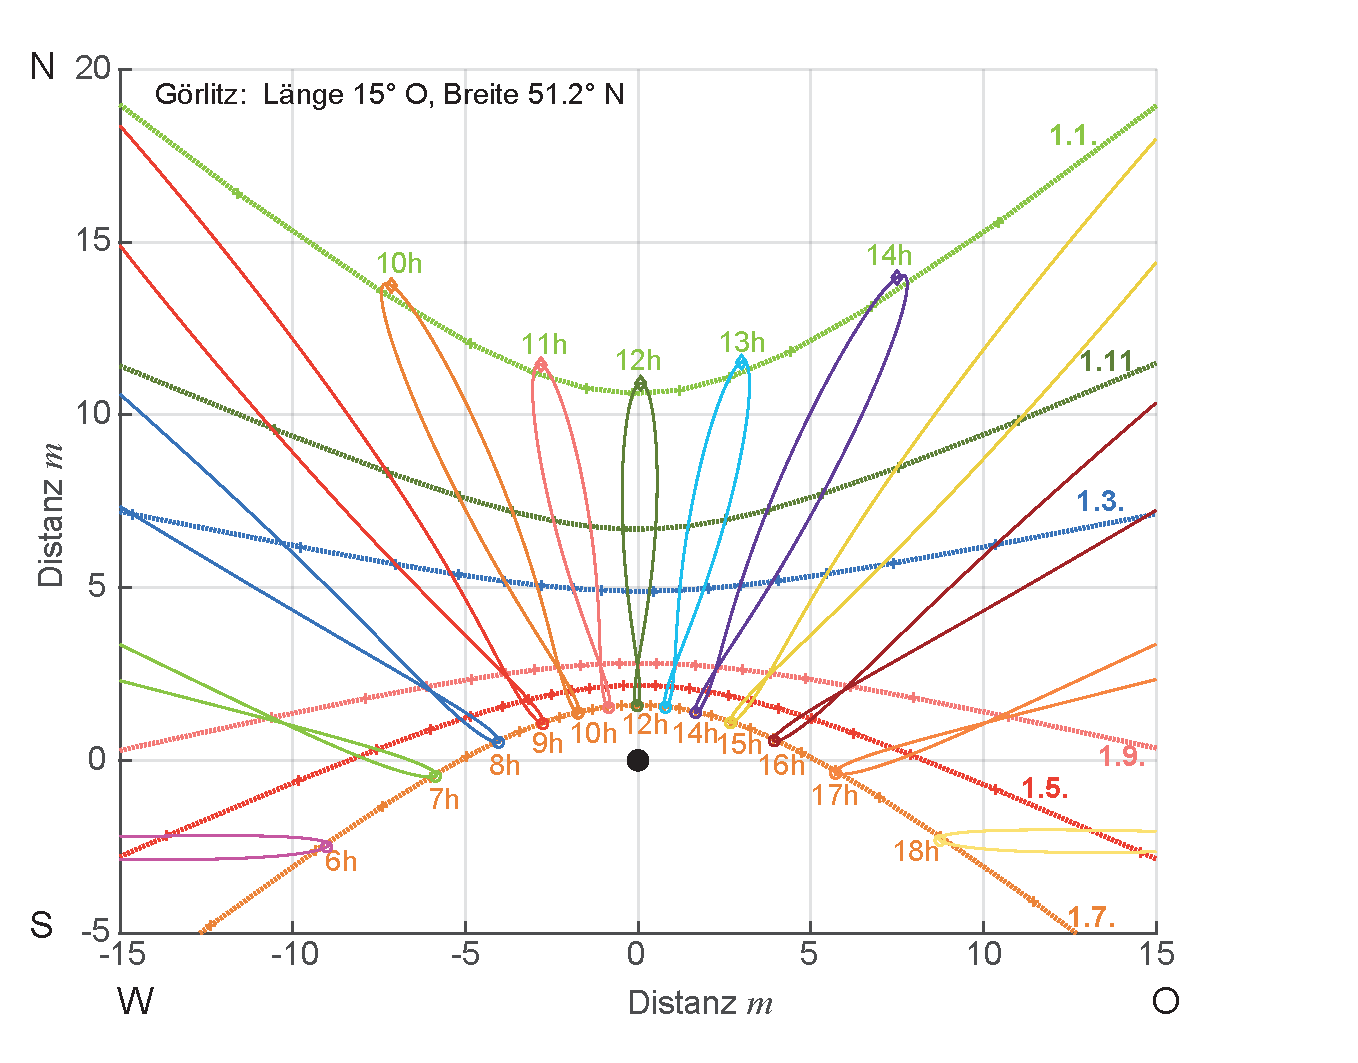
\includegraphics[width=\textwidth]{SonnenuhrAnalem.pdf}%
\caption[Berechnetes Ziffernblatt einer analemmatischen Sonnenuhr f�r G�rlitz.]{Berechnetes Ziffernblatt einer analemmatischen Sonnenuhr f�r G�rlitz. Siehe \mlhmref{SonnenuhrAnalem.m}} %
\label{abb:hm_sundial_lsg03}%
\end{figure}

\medskip \end{sol}
\textcolor{blue} {$\rightarrow$ zur} \probref{hm_VertikalAnalemmaSonnenuhr}.\\
\noindent\rule[1ex]{\textwidth}{0.5pt} \newpage


%-----------------------------------------------------------------------------------------------------------

\begin{sol}{prob:hm_opposition_mars}\label{lsg:hm_opposition_mars} %�bung17
\textbf{Mars-Oppositionen von 2000 bis 2020} \\ \\
Wir berechnen mit Hilfe der Gau�schen Vektoren die Bahnen von Mars und Erde in heliozentrischen Koordinaten und bestimmen die Zeitpunkte, an denen $l_\text{\mars}\!=\!l_\text{\earth}$ ist.
Es ergibt sich dann auch der minimale Abstand $\Delta r$.
Man sieht, dass auf Grund der relativ exzentrischen Bahn des Mars (\figref{hm_mars_opposition_lsg}), die Mars-Oppositionen nahe des Perihels dahingehend ausgezeichnet sind, dass der Mars der Erde besonders nahe kommt.
Wir m�ssen dann noch folgende Parameter berechnen:
\begin{itemize}
	\item Geozentrische Breite des Mars:
	   \begin{equation*}
		  \beta = \arcsin(z_\text{\mars}/\Delta r)
		 \end{equation*}
	\item Deklination des Mars zum Oppositionszeitpunkt \eqref{eq:hm_drehung_x_achse_linear2}:
		  \begin{equation*}
		  \delta = \arcsin(\cos\beta \sin l \sin\epsilon + \sin\beta \cos\epsilon) 
		 \end{equation*}
	\item H�he des Mars in Mitteleuropa zum Oppositionszeitpunkt\footnote{Man beachte, dass $\tau\!=\!0$ gesetzt (also dass Kulmination angenommen) wurde.} \eqref{eq:hm_Alt-Az-Koord}:
	    \begin{equation*}
		  h = \arcsin(\cos\delta\cos\varphi + \sin\delta \sin \varphi)
		 \end{equation*}
	\item Bildwinkel unter dem der Mars zum Oppositionszeitpunkt erscheint:
	     \begin{equation*}
		 \text{Bw} = \arcsin (R_\text{\mars}/ \Delta r)~~\text{mit}~~ R_\text{\mars} \approx 6770\:\text{km}
		 \end{equation*}
\end{itemize}
\begin{figure}[H]
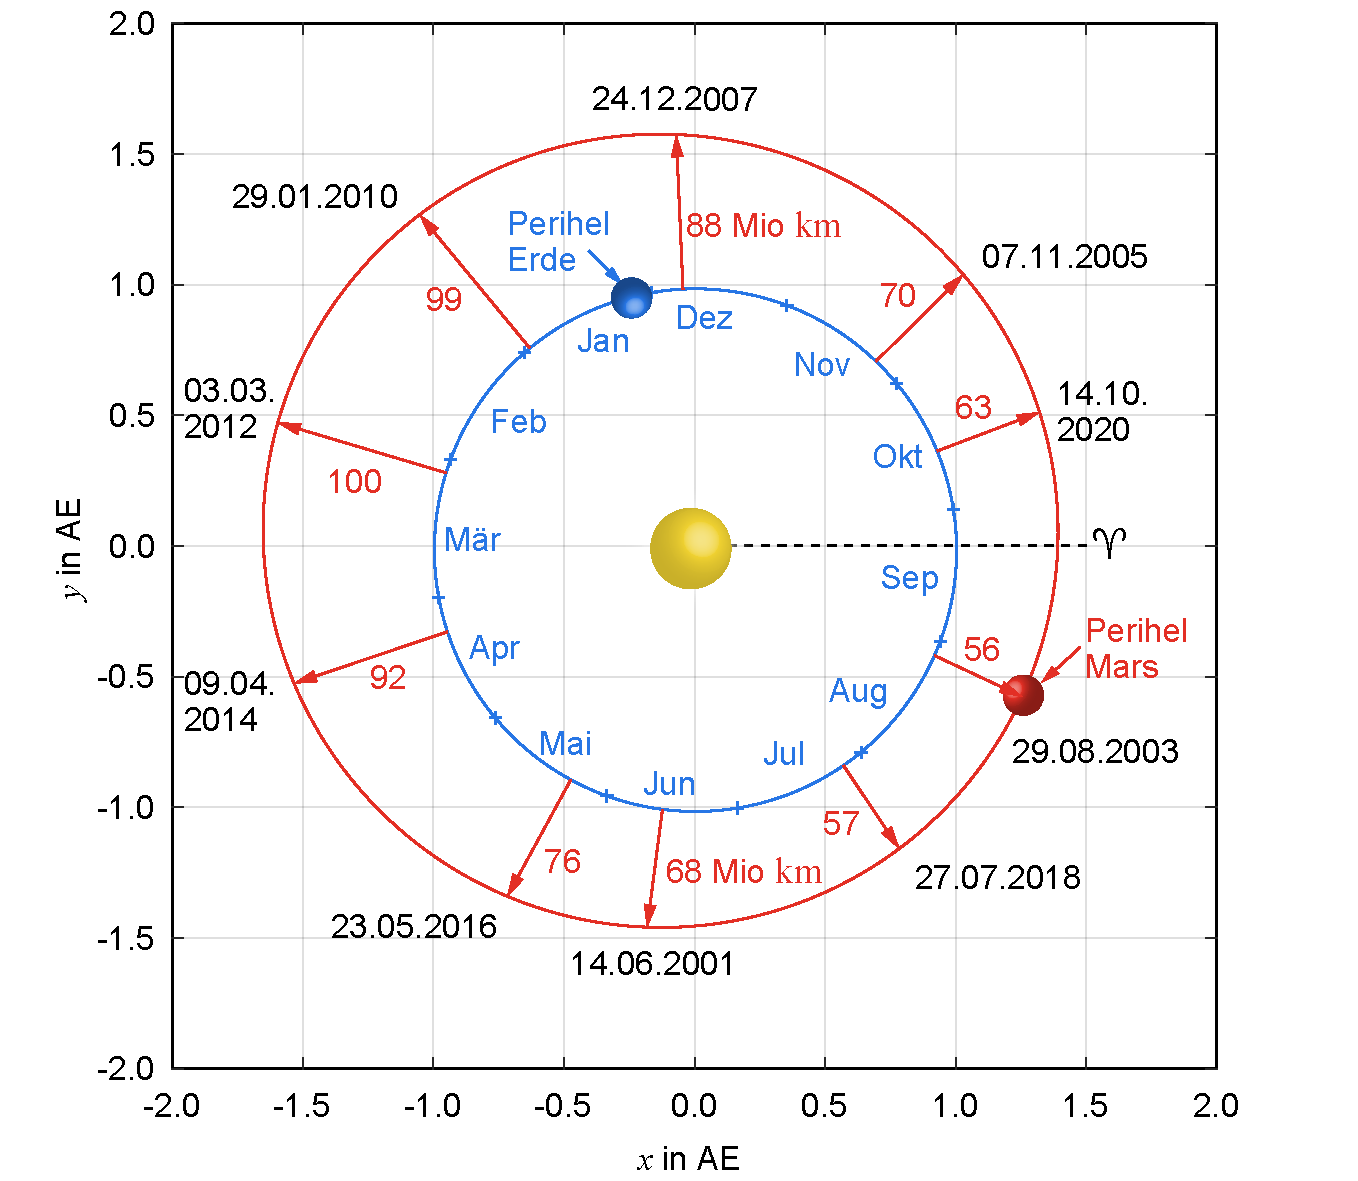
\includegraphics[width=\textwidth]{Mars_Opposition.pdf}%
\caption{Mars-Oppositionen im Zeitraum 2000 bis 2020}%
\label{abb:hm_mars_opposition_lsg}%
\end{figure}

\newpage
\begin{table}
\caption{Berechnung der Mars-Oppositionen von 2001 bis 2040}
\begin{tabular}{lR{1cm}R{1cm}R{1.5cm}R{1.5cm}R{1cm}R{1cm}R{1cm}R{1cm}}
\hline\noalign{\smallskip}
Datum	& $l\,[\degree]$ & $b\,[\degree]$ & $\Delta r\,[10^6\,\text{km}]$ & $R_\text{\mars}\,[10^6\,\text{km}]$ & $\beta\,[\degree]$ & $\delta\,[\degree]$ & $h\,[\degree]$ & $\text{Bw}\,['']$  \\
\noalign{\smallskip}\svhline\noalign{\smallskip}
14.06.2001 & 262.98 &	-1.02 &	67.80 &	219.10 &	-3.29 &	-26.54 &	14.66 &	20.60 \\
28.08.2003 & 335.09 &	-1.78 &	55.60	& 205.80 &	-6.62	& -15.79 &	25.41 &	25.13 \\
08.11.2005 & 45.70	& -0.13	& 70.40	& 218.00 &	-0.39	& 16.17	 &  57.37	& 19.85 \\
25.12.2007 & 93.05  &	1.27  & 88.60	& 235.00 &	3.38 &	26.78	 &  67.98	& 15.77 \\
30.01.2010 & 130.05	& 1.83	& 99.10	& 245.70 &  4.53	& 22.08	 &  63.28	& 14.10 \\
04.03.2012 & 163.78	& 1.69	& 100.40 & 248.00	& 4.17 &	10.23	 & 51.43	& 13.91 \\
10.04.2014 & 199.42 &	0.93	& 92.30	& 241.40	& 2.43	& -5.34	& 35.86	& 15.14 \\
23.05.2016 & 242.17	& -0.40	& 75.60	& 226.50	& -1.21	& -21.78 & 19.42 & 18.47 \\
27.07.2018 &	304.32 &	-1.79 &	57.40	& 208.50 & -6.49 & -25.48	& 15.72	& 24.32 \\
15.10.2020 &	21.49	& -0.87 &	62.70	& 211.20 & -2.94 &	5.65	& 46.85 & 22.28 \\
08.12.2022 &	76.10	& 0.83 &	82.10	& 228.80 &	2.31 &	25.01	& 66.21 &	17.02 \\
16.01.2025 &	116.10 &	1.70 &	96.00 &	242.40 &	4.29 &	25.14 &	66.34 &	14.55 \\
20.02.2027 &	150.93 &	1.81 &	101.00 & 248.10 &	4.46 &	15.31 &	56.51 &	13.83\\
25.03.2029 &	184.71 &	1.31 &	96.60	& 245.10 &	3.31 &	1.17 & 42.37 & 14.46 \\
04.05.2031 &	223.42 &	0.20 &	83.20	& 233.40 &	0.56 &	-15.33 & 25.87 &	16.79 \\
28.06.2033 &	276.69 &	-1.36 &	63.50	& 214.80 &	-4.59 &	-27.86 & 13.34 & 22.00 \\
17.09.2035 &	353.13 &	-1.54 &	57.00	& 206.60 &	-5.60	& -7.87 &	33.33	& 24.50 \\
20.11.2037 &	57.36  &	0.25 &	74.70	& 221.90 &	0.74 & 20.29 &	61.49	& 18.70 \\
03.01.2040 &	101.70 &	1.46 &	91.60	& 238.00 &	3.80 &	26.71 &	67.91 & 15.24 \\
\noalign{\smallskip}\hline\noalign{\smallskip}
\end{tabular}
\label{tab:hm_Mond-Mars-Abstand}
\end{table} 

In \figref{hm_mars_opposition_lsg} sind die Mars-Oppositionen f�r den Zeitraum 2000--2020 jeweils mit Datum und Abstand angegeben.
Man erkennt, dass bei Oppositionen in Periheln�he (z.\,B. am 29.08.2003) der Mars nahezu doppelt so gro� am Himmel erscheint\footnote{Tats�chlich konnte einer der Autoren (MK) am 29.08.2003 die Polkappen des Mars mit einem ZEISS APQ 135 ($5''$ Durchmesser und $2\:$m Brennweite) problemlos beobachten.
Gleich gute Chancen wird man in Europa erst wieder im Jahr 2035 haben.} wie bei Oppositionen in Apheln�he (z.\,B. am 03.03.2012).
Die Mars-Oppositionen f�r den Zeitraum 2001--2040 inklusive der f�r die Berechnung n�tigen Parameter sind in Tabelle \ref{tab:hm_Mond-Mars-Abstand} angegeben.\\

\medskip \end{sol}
\textcolor{blue} {$\rightarrow$ zur} \probref{hm_opposition_mars}.\\
\noindent\rule[1ex]{\textwidth}{0.5pt} \newpage


%-----------------------------------------------------------------------------------------------------------

\begin{sol}{prob:hm_venus_2004_2012}\label{lsg:hm_venus_2004_2012} %�bung18
\textbf{Venustransit-Beobachtungen 2004 und 2012} 

Vorbemerkung:\\
Beide Transits waren eine Jahrhundertereignis. Der n�chste Venustransit wird erst wieder 2117 zu beobachten sein. Wir bereiten mit dieser �bung aber schon mal die Berechnung vor. Ob man allerdings in 2117 noch eine \matlab{} Lizenz erwerben kann, ist nicht mit Sicherheit zu beantworten.

\begin{enumerate}[(a)] 
	\item Wir gehen von \figref{hm_VenusParallax} aus und betrachten den Fall, dass die Venus-Projektionen auf der Sonnenscheibe von den beiden Orten auf der Erde nicht symmetrisch zum Sonnenzentrum liegen.
          �ber die Geometrie der Winkel kann man zeigen, dass folgende Beziehungen gelten:
\begin{align*}
\nu_\text{\astrosun}+\nu_1 &= \nu_\text{\venus} + \nu_2 \\
\Rightarrow \Delta\nu &= \nu_1-\nu_2 ~~,
\end{align*}
woraus mit
\begin{align*}
\frac{\nu_\text{\venus}}{\nu_\text{\astrosun}} &= \frac{a_\text{\earth}}{a_\text{\venus}} \nonumber\\
\end{align*}
die Beziehung f�r die Astronomische Einheit 
\begin{equation}
a_\text{\earth} = \lk\frac{1}{\Delta\nu}\rk \lk\frac{d_\text{eff}}{\frac{a_\text{\earth}}{a_\text{\venus}} - 1}\rk = \frac{1}{\Delta\nu} \frac{d_\text{eff}}{\gamma - 1} \label{lsg:hm_venus_2004_2}
	\end{equation}
folgt.
\smallskip
Wir berechnen den effektiven Abstand $d_\text{eff}$ zwischen Troms� (N) und Canberra (AUS), in dem wir f�r die geographischen Koordinaten der Beobachtungsorte deren geozentrische Koordinaten verwenden.
Die Deklination f�r den Beobachtungsort entspricht dann der geographischen Breite (Abplattung der Erde vernachl�ssigt) und die Rektaszension ist einfach die Sternzeit berechnet nach \eqref{eq:hm_UT_3} zur Beobachtungszeit in UT.
Wir erhalten zu den Beobachtungsorten zwei Positions-Vektoren $\vec{r}_\text{T}$ und $\vec{r}_\text{C}$, deren Differenzvektor $\vec{r}_\text{d} = \vec{r}_\text{T}- \vec{r}_\text{C}$ unter einem Winkel $w$ zum Richtungsvektor Erdmittelpunkt -- Sonne ($\cos\delta\cos\alpha$, $\cos\delta\sin\alpha$, $\sin\delta$) steht.
Wir berechnen den Kosinus dieses Winkel $w$ aus dem Skalarprodukt.
Die effektive L�nge ist dann gegeben durch 
\begin{equation*}
d_\text{eff}=\left| \vec{r}_\text{d} \right|\sin w ~~.
\end{equation*}
F�r die Werte am 06.\,06.\,2012 sind die einzelnen Berechnungen in \mlhmref{VenusMerkurTransit.m} ausgef�hrt und numerisch ergibt sich $d_\text{eff}\!=\!11415 \:\text{km}$. \\
Ein sehr sch�ne Auswertung f�r die Berechnung der AE bei Beobachtung der Transitdauer an zwei Standorten findet sich in \cite{Messmer2004}. \\
\smallskip

	\item Wir gehen nun �ber zu der Auswertung der Transitdaten von nur einem Standort.
          Dazu muss man wie im  Beispiel \ref{bsp:venustransit} ausgef�hrt auf die t�gliche Parallaxe zur�ck greifen.
          Aus der Abbildung des Beispiels \ref{bsp:venustransit} k�nnen wir die folgende Beziehung ableiten:
	\begin{align}
	\frac{\D s_\text{\venus}-\D s_\text{\earth}}{a_\text{\earth}-a_\text{\venus}}&=\frac{\D P_\text{B} - \D s_\text{\earth}}{a_\text{\earth}}~,\nonumber\\
	\Rightarrow \frac{a_\text{\venus}}{a_\text{\earth}-a_\text{\venus}} \lk \frac{\D s_\text{\venus}}{a_\text{\venus}} - \frac{\D s_\text{\earth}}{a_\text{\earth}} \rk &= \frac{\D P_\text{B}}{a_\text{\earth}} ~,\nonumber \\
	\stackrel{\, 1/\D t}{\Rightarrow} \lk\frac{1}{\gamma -1}\rk \lk  \omega_\text{\venus} - \omega_\text{\earth} \rk &= \Omega_\text{B} ~~. \label{lsg:hm_venus_2004_3}
	\end{align}
Dabei haben wir $\gamma\!=\!a_\text{\earth} / a_\text{\venus}$, $\D s_i\!=\!\omega_i a_i \D t$ und $\D P_\text{B}\!=\!\Omega_\text{B} a_\text{\earth} \D t$ benutzt.
\smallskip
Wir berechnen den effektiven Abstand $d_\text{eff}$ f�r die Beobachtungen am 08.06.2004 in Oberkochen ($\phi\!=\!48.8\degree$ N, $\lambda\!=\!10.1\degree$ O) wieder wie oben, indem wir f�r die geographischen Koordinaten der Beobachtungszeitpunkte die geozentrische Koordinaten verwenden.
Die Deklination entspricht dann der geographischen Breite und die Rektaszensionen der Sternzeiten berechnet nach \eqref{eq:hm_UT_3} zum Anfangs- und Endzeitpunkt des Transits.
F�r gemessene Zeiten f�r Transitbeginn 07:16 MESZ $\pm 1$ min und Transitende 13:18 MESZ $\pm 1$ min ergibt sich eine effektive Entfernung von $d_\text{eff}\!=\!4444\:\text{km}$.
Die relative Sehnenl�nge konnte dabei zu 0.775 bestimmt werden (Messdaten MK).
Mit der Berechnungsformel aus dem Beispiel
\begin{equation}
a_\text{\earth}=\lk\frac{d_\text{eff}}{\gamma-1}\rk \lk\frac{1}{{l_\text{S\astrosun}}{b_\text{w\astrosun}}-\Omega_\text{B} T_\text{TR,B }}\rk \label{lsg:hm_venus_2004_4}
\end{equation}
erhalten wir daraus als Mittelwert f�r $\text{AE}\!=\!115\cdot 10^6\:$km.
Tr�gt man den relativen Fehler als Funktion der gemessenen Transitzeit auf, so sieht man, dass schon bei Unsicherheiten in der gemessenen Transitzeit von $60\:\text{s}$ ein Fehler von $20\%$ in der Bestimmung der astronomischen Einheit resultiert (\figref{hm_Kontaktzeit_lsg}a.
Das liegt daran, dass die Abh�ngigkeit von der gemessenen Transitzeit, bei dem gegen Null gehenden Nenner in \eqref{lsg:hm_venus_2004_3} sehr gro� ist (\figref{hm_Kontaktzeit_lsg}b.
Genau so kritisch ist die Messung der Sehnenl�nge $l_\text {S}$ des Transits.
Im Rahmen der Messgenauigkeit ergab sich ein Mittelwert von $115\cdot 10^6\:\text{km} $.\footnote{Der Mittelwert ist tendenziell ein eher zu kleiner Wert, was vermuten l�sst, dass die Messzeit als zu kurz eingesch�tzt wurde.
Es ist au�erordentlich schwierig, am Rand der Sonne genau Beginn und Ende des Transits festzustellen.}
\begin{figure}[H]
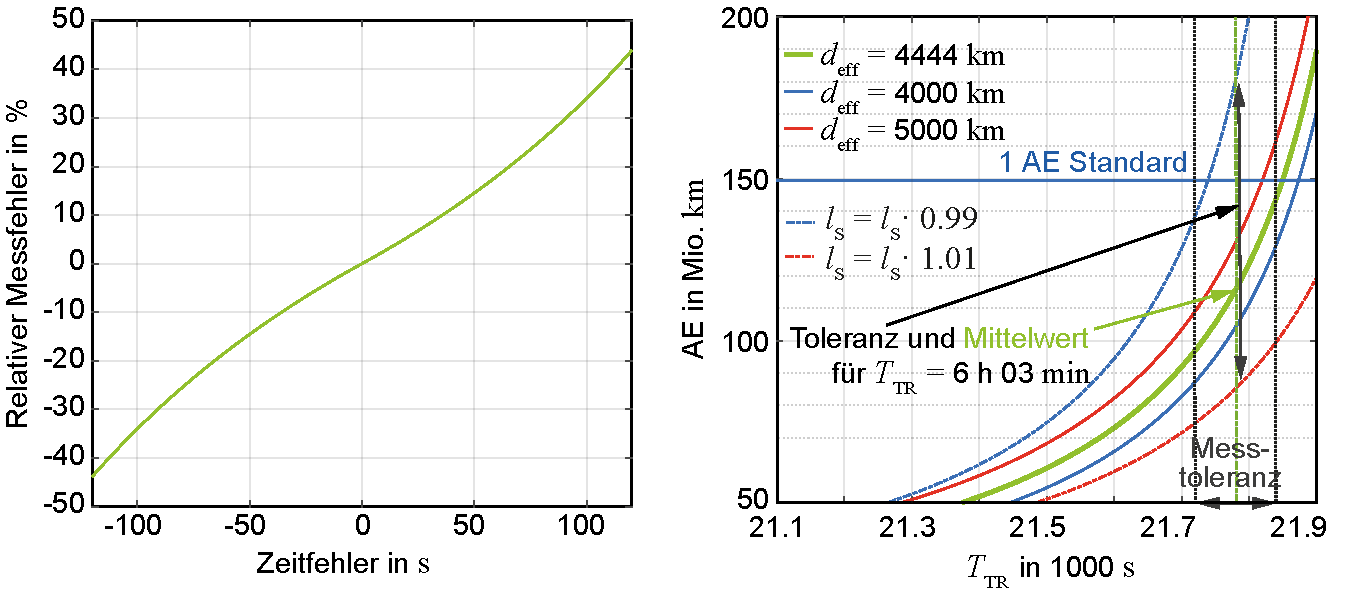
\includegraphics[width=\columnwidth]{KontaktzeitmethodeAE.pdf}%
\caption{Fehler in der Bestimmung der AE bei der Kontaktzeitmethode}%
\label{abb:hm_Kontaktzeit_lsg}%
\end{figure}
Ein verbesserte Auswertung f�r die Berechnung der AE bei Beobachtung der Transitdauer an nur einem Standorten findet sich \cite{Brodbeck2004}. \\

	\item Wir ber�cksichtigen jetzt f�r den Fall, dass die Beobachtung nur an einem Ort der Erde stattfinden kann.
          sowohl die Elliptizit�t der Bahnen, als auch die Neigung der Venusbahn gegen die Ekliptik und die topozentrischen Koordinaten des Beobachters.
          Diese Berechnung geht auf den Astronomen James Short\footnote{James Short (1710--1768) war ein britischer Mathematiker, Optiker und begnadeter Teleskopbauer.
          Wir empfehlen dazu auch den lesenswerten Artikel \cite{Teets2003}, auf dessen Basis die L�sung der �bung strukturiert wurde.} zur�ck, der viele der Messungen von 1761 systematisch auswertete und dessen ermittelte Sonnenparallaxe von $8.65''$ �quivalent zu $a_\text{\earth}\!=\!154.4\cdot 10^6 \:\text{km}$ lange als Referenz f�r die AE galt.
          Die Rechnungen sind im Detail in \mlhmref{VenusMerkurTransit.m} ausgef�hrt.
          Eine Betrachtung f�r n�herungsweise konzentrisch und koplanar angenommene Planetenbahnen kann man in \cite{Messmer2004} bzw. \cite{Brodbeck2004} finden. \\
Um den Transit in seiner allgemeinen Form zu berechnen, m�ssen wir zwei KOS zueinander in Beziehung setzen:
\begin{enumerate}[A.]
	\item Das GA(sf) KOS (\figref{hm_venustransit_lsg_2a}), was f�r den Beobachter des Transits das ausgezeichnete KOS ist und folgenderma�en definiert ist:
	Die $x'$-Achse zeigt zum Fr�hlingspunkt und beh�lt ihre Richtung im Raum bei, die $z'$-Achse ist die Rotationsachse der Erde.
	\begin{enumerate}[1.]
	\item Die t�gliche Rotation der Erde beschreiben wir mit 
\begin{equation}
\theta = \theta_0 + \frac{15\degree}{\text{h}}\, (t-t_0)~~,
\label{eq:hm_venustr_d_3}
\end{equation}
worin $\theta_0\!=\!\GMST$ und die Zeiten $t$, $t_0$ in UT angegeben werden.
$t_0$ soll dabei die Zeit der Transitmitte sein.
\begin{figure}[H]
	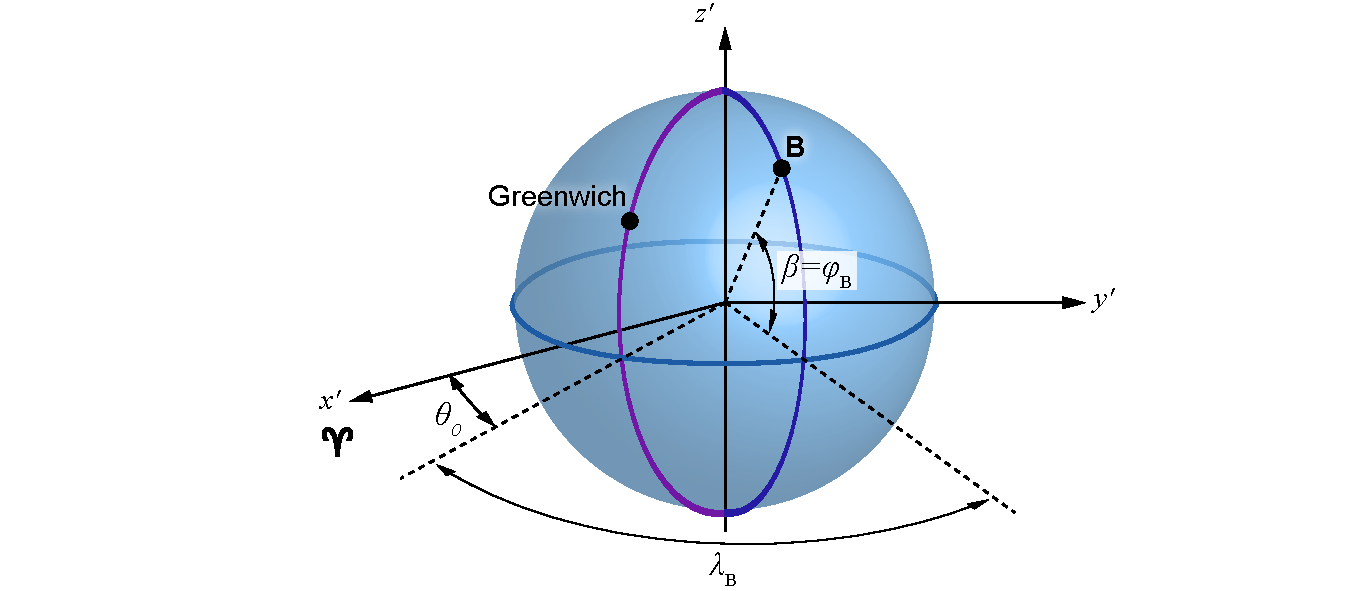
\includegraphics[width=\textwidth]{VenustransitKS.pdf}%
	\caption[Koordinatensystem des Beobachters beim Venustransit.]{Koordinatensystem ($x'$-$y'$-$z'$) des Beobachters beim Venustransit}%  
	\label{abb:hm_venustransit_lsg_2a}%
\end{figure}
	\item F�r die Koordinaten $\vec{r}'$ rechnen wir die geographischen Koordinaten $\varphi_\text{B}$, $\lambda_\text{B}$ eines Beobachters B in geozentrisch-�quatoriale Koordinaten um, wobei die Abplattung der Erde vernachl�ssigt wird und deshalb $\beta\!=\!\varphi_\text{B}$ ist.
          Damit gilt 
\begin{equation}
\vec{r}' = \lk\begin{matrix} x' \\ y' \\ z'\end{matrix}\rk = \mathbb{R}_\text{\earth}\,\lk\begin{matrix} \cos\beta\cos(\theta+\lambda_\text{B})\\ \cos\beta\sin(\theta + \lambda_\text{B})\\ \sin\beta \end{matrix}\rk ~~.
\label{eq:hm_venustr_d_2}
\end{equation}
\end{enumerate}	
	\begin{figure}[H]
	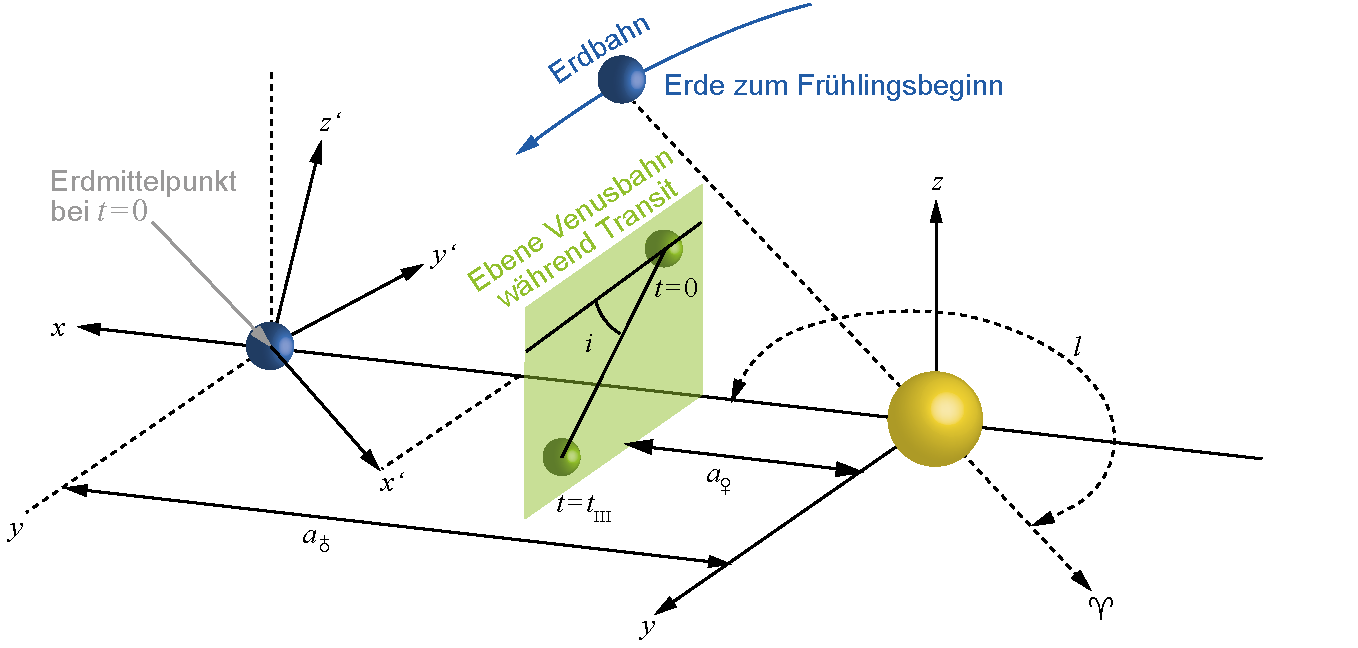
\includegraphics[width=\textwidth]{VenustransitHelioKS.pdf}%
	\caption[Beziehungen der Koordinatensysteme beim Venustransit.]{Beziehung des heliozentrischen Koordinatensystems ($x$, $y$, $z$) und des Koordinatensystems des Beobachters ($x'$, $y'$, $z'$) beim Venustransit}% 
	\label{abb:hm_venustransit_lsg_2b}%
	\end{figure}
	
	\item Das HE-KOS, welches f�r die Beschreibung der Planetenbewegung das geeignete ist.
          Bei diesem zeige die $x$-Achse nicht zum Fr�hlingspunkt, sondern zum Mittentransitzeitpunkt genau zum Erdmittelpunkt.
	\item Die Beziehung zwischen den kartesischen Koordinaten beider KOS ergibt sich nach \figref{hm_venustransit_lsg_2b} gem��:
	\begin{enumerate}[1.] 
	\item Translation
\begin{align}
	\vec{r} &= \mathbb{R}_z(-l)\,\mathbb{R}_y(-\epsilon)\,\vec{r}' + \vec{r}_\text{\earth\astrosun} \nonumber\\
	\smallskip
	\lk\begin{matrix} x \\ y \\ z \end{matrix}\rk &= \lk\begin{matrix} \cos l & \sin l & 0 \\ -\sin l & \cos l & 0 \\ 0 & 0 & 1\end{matrix}\rk \lk\begin{matrix} 1 & 0 & 0 \\ 0 & \cos\epsilon & \sin\epsilon \\ 0 & -\sin\epsilon & \cos\epsilon \end{matrix}\rk \lk\begin{matrix} x' \\ y' \\ z' \end{matrix}\rk + \lk\begin{matrix} a_\text{\earth} \\ 0 \\ 0 \end{matrix}\rk ~~. \label{eq:hm_venustr_d_1}
\end{align}
\item W�hrend der halben Dauer des Transits bewegt sich die Erde mit ihrer Winkelgeschwindigkeit $\omega_\text{\earth}$ weiter um die Sonne.
  Wir nehmend etwas vereinfachend an, dass diese Bewegung in der betrachtet kurzen Zeitspanne nur entlang der $y$-Achse erfolgt.
  D.\,h. wir haben 
\begin{equation}
\Delta \vec{r} = \lk\begin{matrix} 0 \\ \omega_\text{\earth}t \\ 0 \end{matrix}\rk ~~.
\label{eq:hm_venustr_d_4}
\end{equation}
Addiert man \eqref{eq:hm_venustr_d_4} und \eqref{eq:hm_venustr_d_1}, erh�lt man mit \eqref{eq:hm_venustr_d_2} und \eqref{eq:hm_venustr_d_3} f�r $\vec{r}'$ die Koordinaten des Beobachters zu einem beliebigen Zeitpunkt $t$ w�hrend des Transits.
\end{enumerate}
\end{enumerate}
\begin{figure}[H]
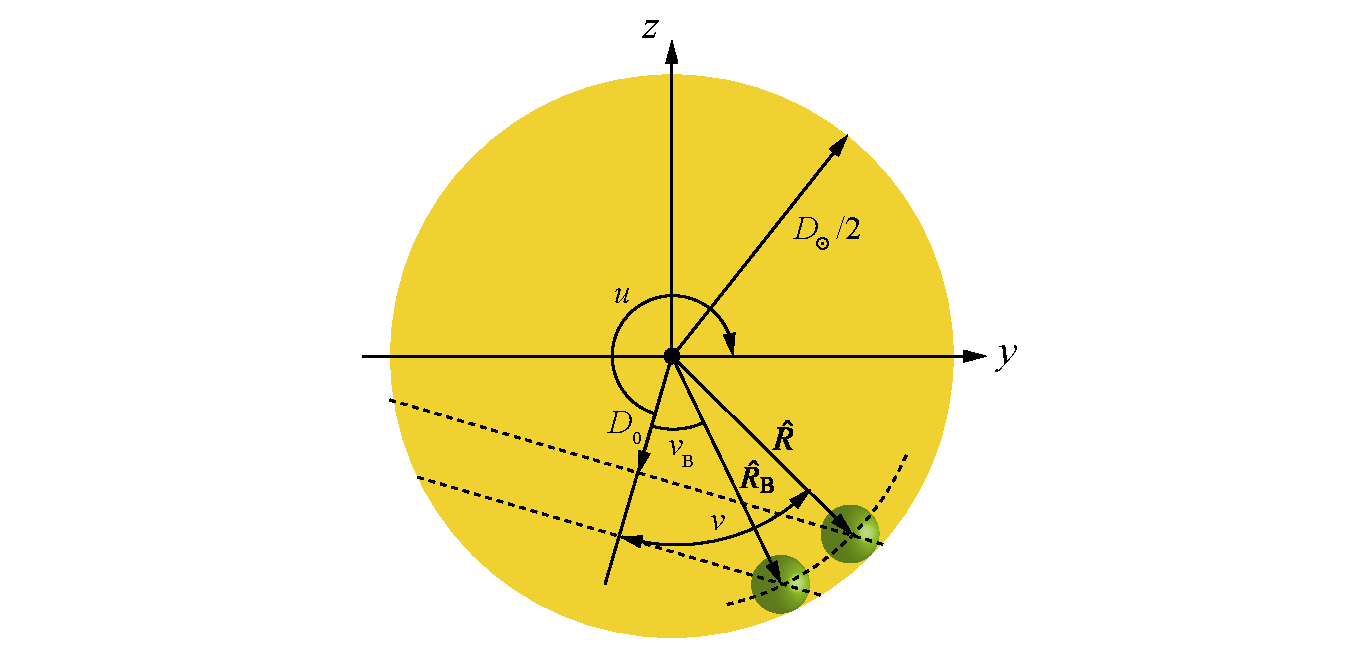
\includegraphics[width=\textwidth]{VenustransitGeometrie.pdf}%
\caption{Geometrie des Venustransits}%
\label{abb:hm_venustransit_lsg_3}%
\end{figure}

Wir betrachten nun als angenommener Beobachter im Erdmittelpunkt die Position der Venusprojektion vor der \anf{Sonnenscheibe} in \figref{hm_venustransit_lsg_3}.
Dabei m�ssen wir uns noch einmal klarmachen, dass zu jedem Zeitpunkt des Transits Erdmittelpunkt, Venusmittelpunkt und der Mittelpunkt des Venus-Projektionsscheibchens auf der Sonne auf einer Linie liegen.
F�r die Projektionsposition $\vec{r}_\text{P,0}$ (Mitte des Transits $t\!=\!0$) ergibt sich dann f�r die Position der Venus im $x,y,z$-KOS:
\begin{equation}
\gamma \lk \vec{r}_\text{\venus,0} - \vec{r}_\text{P,0} \rk =  \lk \vec{r}_\text{\earth,0} - \vec{r}_\text{P,0}\rk ~,
\label{eq:hm_venustr_d_5}
\end{equation}
worin $\gamma = a_\text{\earth}/a_\text{\venus}$ ist und 
\begin{equation*}
\vec{r}_\text{\earth,0} = \lk\begin{matrix} a_\text{\earth} \\ 0 \\ 0\end{matrix}\rk ~~\text{und}~~ \vec{r}_\text{P,0} = \lk\begin{matrix} 0 \\ D_0\cos u \\ D_0\sin u\end{matrix}\rk
\end{equation*}
jeweils die Positionen des Erdmittelpunktes und die Mitte des Projektionsscheibchens zum Transitmittenzeitpunkt sind.
F�r einen sp�teren Zeitpunkt $t$, z.\,B. dem Zeitpunkt des sogenannten 3. Kontakts $t_\text{III}$ gilt analog
\begin{equation}
\gamma \lk \vec{r}_\text{\venus,III} - \vec{r}_\text{P,III} \rk = \lk \vec{r}_\text{\earth,III} - \vec{r}_\text{P,III} \rk ~,
\label{eq:hm_venustr_d_6}
\end{equation}	
worin
\begin{equation*}
\vec{r}_\text{P,III} = \lk\begin{matrix} 0 \\ \hat{R}\cos(u+v) \\ \hat{R}\sin(u+v)\end{matrix}\rk ~~\text{mit}~~ \hat{R} = \frac{D_\text{\astrosun}}{2} - R_\text{P} ~~.
\end{equation*}	
Hierin ist $R_\text{P}$ der Radius des Projektionsscheibchens auf der Sonne und $D_\text{\astrosun}$ der Durchmesser der Sonne, jeweils in Winkelma�en angegeben.
F�r die Koordinaten $\vec{r}_\text{\venus,III}$ und $\vec{r}_\text{\earth,III}$ m�ssen wir die planetare Bewegung ber�cksichtigen (\figref{hm_venustransit_lsg_2b}), so dass dann folgt:
\begin{align}
	\vec{r}_\text{\earth,III} &= \lk\begin{matrix} a_\text{\earth} \\ \omega_\text{\earth} t_\text{III} \\ 0\end{matrix}\rk ~~, \nonumber\\
	\vec{r}_\text{\venus,III} &= \vec{r}_\text{\venus,0} + a_\text{\venus} \omega_\text{\venus} t_\text{III}\,\lk\begin{matrix} 0 \\ \cos i \\ -\sin i\end{matrix}\rk ~~. \label{eq:hm_venustr_d_7}
\end{align}	
Darin haben wir die Bewegung der Erde entlang der Richtung der $y$-Achse und die der Venus in der $y,z$-Ebene angenommen.
Die Bahnneigung der Venus gegen�ber der Ekliptik ist damit ber�cksichtigt, $\vec{r}_\text{\venus,0}$ ist durch \ref{eq:hm_venustr_d_5} gegeben.
Mit \eqref{eq:hm_venustr_d_5} bis \eqref{eq:hm_venustr_d_7} haben wir den Transit nun vollst�ndig f�r einen \anf{hypothetischen} Beobachter im Erdmittelpunkt beschrieben.
Wir wollen jetzt die Transitzeit bzw. die Zeit des 3. Kontakts bestimmen.
Wir erhalten aus der $y$-Komponente der Gleichung \eqref{eq:hm_venustr_d_6}
\begin{equation}
\sin u = \frac{a_\text{\venus} (\omega_\text{\earth} - \omega_\text{\venus}\cos i) }{(a_\text{\earth} - a_\text{\venus})\,\sqrt{\hat{R}^2 - D_0^2}}\,t_\text{III}
\label{eq:hm_venustr_d_8}
\end{equation}
und analog f�r die $z$-Komponente
\begin{equation}
\cos u = \frac{a_\text{\venus} \omega_{\venus} \sin i}{(a_\text{\earth} - a_\text{\venus})\,\sqrt{\hat{R}^2 - D_0^2}}\,t_\text{III} ~~.
\label{eq:hm_venustr_d_9}
\end{equation}	
Wegen $\cos^2 u + \sin^2 u\!=\! 1$ folgt aus \eqref{eq:hm_venustr_d_8} und \eqref{eq:hm_venustr_d_9}
\begin{equation*}
t_\text{III} = \lk \frac{a_\text{\earth}}{a_\text{\venus}} - 1 \rk\,\sqrt{\frac{\hat{R}^2 - D_0^2}{\omega_\text{\venus}^2 + \omega_\text{\earth}^2 - 2\omega_\text{\venus} \omega_\text{\earth} \cos i}} ~~.
\end{equation*}	
Man erkennt, dass f�r die im Beispiel \ref{bsp:venustransit} gemachte N�herung der koplanaren Bahnen sich tats�chlich die gesamte Transitzeit n�herungsweise zu	
\begin{equation*}
T_\text{TR} = 2t_\text{III} \approx (\gamma -1)\,\lk\frac{l_\text{s}}{\omega_\text{\venus} - \omega_\text{\earth}}\rk
\end{equation*}
ergibt.
Jetzt gehen wir vom Erdmittelpunkt zu einem Beobachter auf der Erdoberfl�che bei $(\varphi_\text{B},\lambda_\text{B})$ �ber.
Wir wissen aus der Geometrie, dass dessen beobachtete Zeit des 3. Kontakts $t_\text{III}^\text{(B)}\!\neq\! t_\text{III}$ ist.
Ebenso hat f�r ihn das Bild der Venus auf der Sonne bei $t\!=\!t_\text{III}^\text{(B)}$ andere Koordinaten als f�r den gedachten Beobachter im Erdmittelpunkt.
\begin{equation}
\vec{r}_\text{P,III}^\text{(B)} = \lk\begin{matrix} 0 \\ y_\text{P} \\ z_\text{P}\end{matrix}\rk ~~\text{mit}~~ \hat{R}_\text{B} = \hat{R} = \sqrt{y_\text{P}^2 + z_\text{P}^2} ~~.
 \label{eq:hm_venustr_d_10}
\end{equation}
Die Position des Beobachters auf der Erdoberfl�che zum Zeitpunkt $t\!=\!t_\text{III}^\text{(B)}$ ist demnach durch
\begin{equation}
\vec{r}_\text{\earth,III}^\text{(B)} = \lk \begin{matrix} x^\text{(B)} \\ y^\text{(B)} \\ z^\text{(B)} \end{matrix} \rk + \lk \begin{matrix} 0 \\ \omega_\text{\earth}t_\text{III}^\text{(B)} \\ 0 \end{matrix}\rk ~~.
\label{eq:hm_venustr_d_11}
\end{equation}
gegeben.
Die Position der Venus zu diesem Zeitpunkt ergibt sich aus \eqref{eq:hm_venustr_d_7} zu
\begin{equation}
\gamma \lk \vec{r}_\text{\venus,III}^\text{(B)} - \vec{r}_\text{\venus,0}^\text{(B)} \rk = \omega_\text{\venus} t_\text{III}^\text{(B)}\,\lk\begin{matrix} 0 \\ \cos i \\ -\sin i \end{matrix}\rk ~~.
\label{eq:hm_venustr_d_12}
\end{equation}
Der Vektor $\vec{r}_\text{\venus,III}^\text{(B)} - \vec{r}_\text{P,III}^\text{(B)}$ muss wiederum ein konstantes Vielfaches $k$ des Vektors $\vec{r}_\text{\earth,III}^\text{(B)} - \vec{r}_\text{P,III}^\text{(B)}$ sein, wie man sich leicht geometrisch klarmachen kann.
Wir erhalten aus der $x$-Komponente $k\!=\!a_\text{\venus}/x^\text{(B)}$, worin $x^\text{(B)}$ die Koordinate der Beobachterposition im kartesischen $x,y,z$ KOS zur Zeit $t_\text{III}^\text{(B)}$ ist.
Damit f�gen wir eine messbare L�ngendimension in das Gleichungssystem ein.
Analog erh�lt man f�r die $y$- und $z$-Komponenten von \eqref{eq:hm_venustr_d_10}
\begin{align*}
	y_\text{P} &= M + Nt_\text{III}^\text{(B)}~~,\\
	z_\text{P} &= P + Qt_\text{III}^\text{(B)}
\end{align*}
mit
\begin{align}
	M &= \frac{(\gamma-1)x^\text{(B)}\,D_0\cos u - y^\text{(B)}}{x^\text{(B)}/a_\text{\venus} - 1} ~~, \label{eq:hm_venustr_d_13} \\
	N &= \frac{x^\text{(B)}\omega_\text{\venus} \,\cos i - \omega_\text{\earth}}{x^\text{(B)}/a_\text{\venus} - 1} ~~, \nonumber\\
	P &=  \frac{(\gamma-1)x^\text{(B)}\,D_0\sin u - z^\text{(B)}}{x^\text{(B)}/a_\text{\venus} - 1} ~~, \nonumber \\
	Q &= \frac{x^\text{(B)} \omega_\text{\venus}\,\sin i}{x^\text{(B)}/a_\text{\venus} - 1} ~~. \nonumber
\end{align}
Wegen $y_\text{P}^2 + z_\text{P}^2\!=\!\hat{R}^2$ folgen schlie�lich die Relationen
\begin{align}
	\hat{R}^2 &= \lk M + Nt_\text{III}^\text{(B)}\rk^2 + \lk P - Qt_\text{III}^\text{(B)}\rk^2 ~~, \label{eq:hm_venustr_d_14} \\
	R^2 &= M^2 + 2NMt_\text{III} + N^2 t_\text{III}^2 + P^2 - 2PQt_\text{III} + Q t_\text{III}^2  ~~,\nonumber \\
	0 &= t_\text{III}^2 \lk N^2 + Q^2 \rk^2 + 2t_\text{III} (MN - PQ) + M^2 + P^2 - \hat{R}^2  ~~,\nonumber\\
	t_\text{III}^\text{(B)} &= -(MN - PQ) + \sqrt{(MN - PQ)^2 + \hat{R} - M^2 - P^2}  ~~.\nonumber
\end{align}
Damit hat man f�r einen Beobachter auf der geographischen Position $\varphi_\text{B},\lambda_\text{B}$ die Zeitdifferenz $t_\text{III}^\text{(B)} - t_\text{III}$ bei der Beobachtung des 3. Kontakts gegen�ber einem hypothetischen Beobachter im Erdmittelpunkt erhalten.
Hat man zwei Beobachter an zwei Orten, so kann man den hypothetischen Beobachter im Erdmittelpunkt eliminieren und betrachtet nur die Messungen der beiden Beobachter auf der Erdoberfl�che.
In $M$, $N$, $P$ und $Q$ sind mit Ausnahme von $a_\text{\venus}$ alle anderen Gr��en bekannt, also $D_0$, $u$, $\hat{R}$, $\omega_\text{\venus}$, $\omega_\text{\earth}$, $\gamma$ und $i$.
Man kann daher �ber einen Fit an $t_\text{III}^\text{(B)}(a_\text{\venus})$ f�r die Zeitdifferenz zweier Beobachtungssituationen den Abstand der Venus bestimmen und �ber das 3. Keplergesetz die Astronomische Einheit berechnen.\\
Sehr instruktiv ist eine "`Vorw�rtsrechnung"', d.h. eine Berechnung der relativen geozentrisch-�quatorialen Koordinaten von Sonne und Venus oder der entsprechenden topographisch-horizontalen Koordinaten (Achtung: hier wirklich topographische Koordinaten verwenden !) mit den heute verf�gbaren Daten aus der St�rungsrechnung.
Siehe auch Zusatzaufgabe \ref{prob:hm_Zusatz_VenusTransit_Vorwaerts}.
Ergebnisse daraus sind im hier f�r den Venustransit von 2004 angegeben (\mscr~\mlhmref{VenusTransit01.m} und \mlhmref{VenusTransit02.m}:). \\
\vspace{0.5 cm}
\begin{tabular}{L{4cm}R{2cm}R{2cm}}
\hline\noalign{\smallskip}
Ort & $t_\text{III}^\text{(B)} - t_\text{III}$ (berechnet) & beobachtet \\
\noalign{\smallskip}\svhline\noalign{\smallskip}
Oberkochen & $-1\:\text{min}\,12\:\text{s}$ & $-1\:\text{min}\,11\:\text{s}$ \\
Troms� & $-1\:\text{min}\,12\:\text{s}$ & \\
Canberra   &  $6\:\text{min}\,12\:\text{s}$ & \\
\end{tabular} 
\vspace{1 cm}
\\
Bemerkungen:
\begin{itemize}
	\item Bemerkung 1\\
Will man die Methode f�r den Transit an nur einem Standort benutzen, so muss man \eqref{eq:hm_venustr_d_14} etwas modifizieren.
Es ist relativ einsichtig, dass die Koordinaten $x^\text{(B)}$, $y^\text{(B)}$ und $z^\text{(B)}$ von $M$, $N$, $P$ und $Q$ von $t_\text{III}^\text{(B)}$ abh�ngen und zu einer bestimmten Zeit berechnet werden m�ssen (\ldots Unterschied zwischen UT und ET beachten!).
Die Gleichungen \eqref{eq:hm_venustr_d_14} sind dann vom Typ
\begin{equation*}
t_\text{III}^\text{(B)} = f(t_\text{III}^\text{(B)},a_\text{\venus})~~,
\end{equation*}
die numerisch nach $a_\text{\venus}$ gel�st werden kann.\\
\item Bemerkung 2\\
Eine v�llig analoge und gleichzeitig sehr instruktive Betrachtung kann man anstellen, wenn man berechnet wie der Venusschatten die Erde trifft.
Diese Methode ist ausf�hrlich in \cite{Backhaus2012} mit Daten f�r den Venustransit von 2012 beschrieben.\\
\item Bemerkung 3\\
Mit zuk�nftigen Marsmissionen wird man nicht bis zum n�chsten Venustransit warten m�ssen, um wieder einen Planeten vor der Sonne vor�berziehen zu sehen.
Nat�rlich gelten alle bisher gemachten �berlegungen auch f�r einen Beobachter auf dem Mars.
Dieser kann dann nat�rlich auch beobachten, wie unsere Erde und ihr Mond vor der Sonne vor�berziehen.
Das letzte Ereignis dieser Art war am 11. Mai 1984 und das n�chste ist am 10.November 2084.
Wir sind aber nicht sicher, ob bereits jetzt Anmeldungen entgegen genommen werden.
Wir empfehlen das mit dem \mscr~\mlhmref{InnerePlaneten.m} \bzw \mlhmref{VenusTransit01.m} zu �berpr�fen.
F�r eine genauere Rechnung der Transitzeiten benutzen Sie die Koordinatenberechnungen nach der St�rungstheorie, d.h. die Funktionen \mlhmiref{SonneExakt.m} und \mlhmiref{MarsExakt.m}.
Siehe auch Zusatzaufgabe \ref{prob:hm_Zusatz_ErdeTransit_from_Mars}.\\
\end{itemize}
\end{enumerate}
\medskip \end{sol}
\textcolor{blue} {$\rightarrow$ zur} \probref{hm_venus_2004_2012}.\\
\noindent\rule[1ex]{\textwidth}{0.5pt} \newpage


%-----------------------------------------------------------------------------------------------------------

\begin{sol}{prob:hm_jupiterbedeckung_venus} \label{lsg:hm_jupiterbedeckung_venus} %�bung19
\textbf{Jupiterbedeckung durch die Venus am 22.11.2065} \\ \\
Die Rechnungen sind im Detail in \mlhmref{PlanetenbahnenKepler.m} ausgef�hrt. \\

\begin{figure}[H]
\begin{minipage}{\textwidth}
\leftfigure{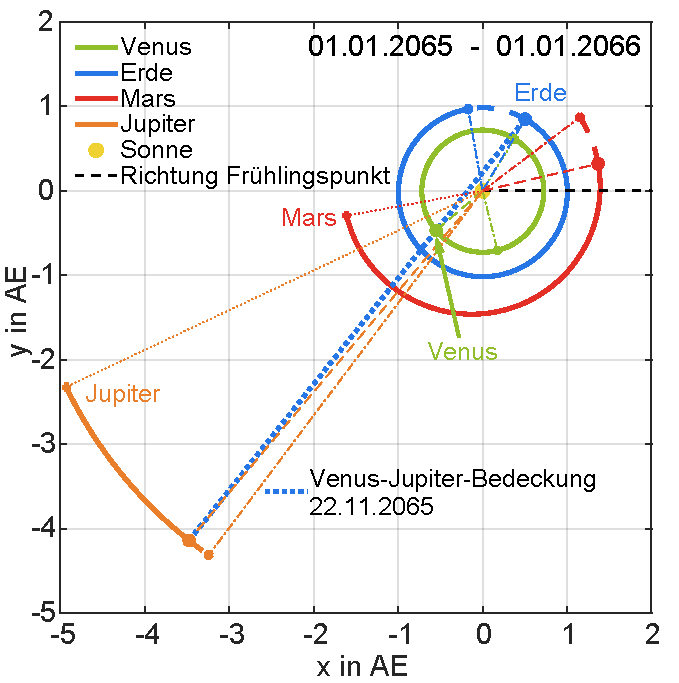
\includegraphics[width=0.5\textwidth]{JupiterBedeckung.pdf}}
\hspace{\fill}
\rightfigure{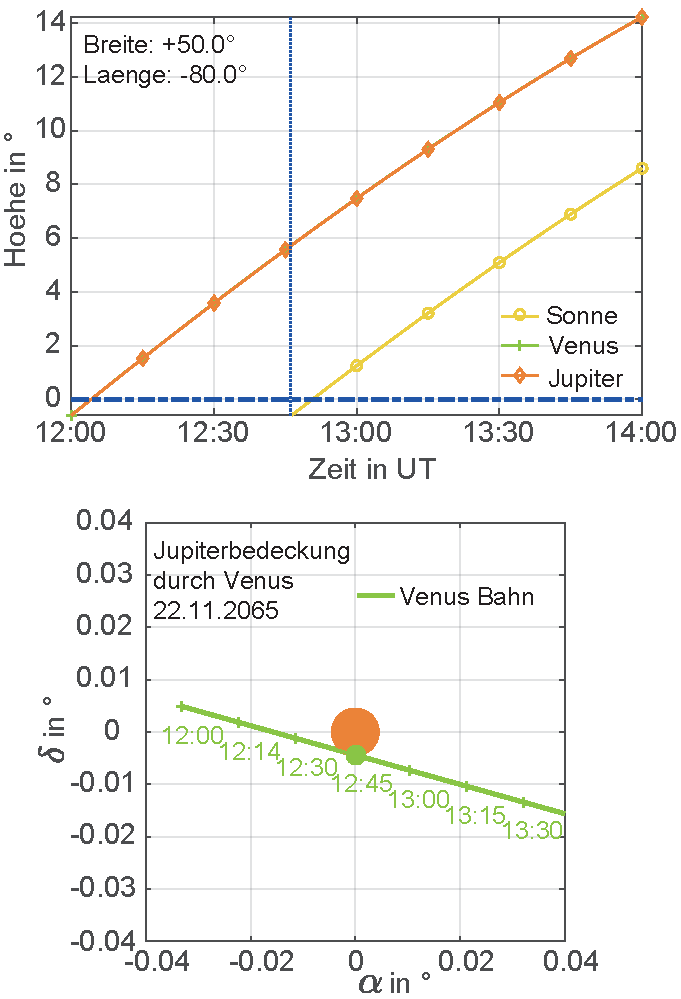
\includegraphics[width=0.5\textwidth]{JupiterVenus.pdf}}
\leftcaption{Konstellation der Planeten am 22.11.2065}\label{abb:hm_JupiterBedeckung_lsg}
\rightcaption{Jupiterbedeckung durch Venus am 22.11.2065}\label{abb:hm_JupiterVenus_lsg}
\end{minipage}
\end{figure}

Aufgrund der erforderlichen Pr�zision wurden die im \matlab{} Programm die hinterlegten Routinen \mlhmiref{VenusExakt.m} und \mlhmiref{JupiterExakt.m} f�r die Berechnung der Planetenpositionen benutzt.
Diese auf den Reihenentwicklungen der St�rungstheorie entwickelten Routinen wurden \cite{Montenbruck1999} entnommen und liefern Genauigkeiten von besser als 10 Bogensekunden �ber den Zeitraum von ca. 50 Jahren.\\
Leider ist die Bedeckung des Jupiters durch die Venus nicht ganz vollst�ndig und noch dazu sehr ung�nstig zu beobachten, da beide Planeten einen relativ geringen Winkelabstand zur Sonne haben.
Am ehesten hat man eine Chance in Nordamerika.

\medskip \end{sol}
\textcolor{blue} {$\rightarrow$ zur} \probref{hm_jupiterbedeckung_venus}.\\
\noindent\rule[1ex]{\textwidth}{0.5pt} \newpage


%%%-----------------------------------------------------------------------------------------------------------

\subsection{�bungen zu Himmelsbeobachtungen von anderen Planeten aus}

\medskip

%-----------------------------------------------------------------------------------------------------------

\begin{sol}{prob:hm_erdaufgang_von_mond} \label{lsg:hm_erdaufgang_von_mond} %�bung20
\textbf{Kann man einen Erdaufgang vom Mond aus sehen?} \\ \\
Als erste Reaktion w�rde man sagen, dass auf dem Mond keine Erdauf- bzw. unterg�nge beobachtet werden k�nnen, da ein Beoabachter auf der Mondvorderseite wegen der gebundenen Rotation (\vgl auch L�sung \ref{lsg:hm_erdrotation}) immer die Erde sieht, wenn auch in verschiedenen Beleuchtungsphasen, so wie wir den Mond sehen.
Diese Behauptung gilt aber nur f�r eine exakt kreisf�rmige Bahn.
Auf Grund der relativ starken Elliptizit�t der Mondbahn und der daraus folgenden unterschiedlichen Geschwindigkeiten, zeigt der Mond der Erde immer ein leicht anderes Antlitz.
Er \anf{sch�ttelt} sozusagen den Kopf (Wir hoffen, dass dies nicht als Missfallen gegen�ber den hier gemachten physikalischen Betrachtungen gedeutet werden muss.).
Dieser Effekt ist schon seit dem Mittelalter als \emph{Libration} bekannt.
Die Libration kann einfach abgesch�tzt werden, indem man das Erde-Mond-System als ZKP betrachtet und die maximale Differenz von wahrer und mittlerer Anomalie berechnet.\\
Mit den Werten f�r die Exzentrizit�t $e_\text{Mond}\!=\!0.0549$ ergibt sich mit den ersten Termen der Mittelpunktsgleichung \eqref{eq:hm_mpglg_nu-M}, wenn f�r die mittlere Anomalie $M_\text{Mond} (t)\!= \!134.96\degree + 13.06\degree \, t \; \text{in} [\degree/\text{d}$] der Wert $90\degree$ oder $270\degree$ eingesetzt wird (der Zeitpunkt $t$ spielt f�r uns jetzt keine Rolle):
\begin{equation*}
	\delta \,l_\text{lib} = C_\text{Mond,max} \approx \upsilon - M_\text{Mond,max} = 2e_\text{Mond} + \frac{5}{5}e_\text{Mond}^3\! + \ldots \approx 0.11 \approx 6.3\degree ~~.
\end{equation*}
Die tats�chliche Libration betr�gt etwa $7.9\degree$.
Der Unterschied von ca. $1.6\degree$ kommt durch den zus�tzlichen Einfluss der Sonne zustande.
Die Erde erscheint vom Mond betrachtet unter einem Winkel 
\begin{equation*}
	2\alpha = \arctan \lk\frac{R_{\earth}}{a_{{\earth}\text{Mond}}} \rk \approx 1.9\degree ~~, 
\end{equation*}
was deutlich kleiner ist als $\delta l_\text{lib}$.
Man kann also vom Mond aus den Erdaufgang sehen, vorausgesetzt man befindet sich in den \anf{Randbereichen} des Mondes (bei selenographische L�ngen um $90\degree$) oder in einem Raumschiff (\probref{hm_erdaufgang_von_apollo}).
Der Landeplatz von Apollo 11 war allerdings bei bei einer selenographischen Position von $0\degree$N und $23.5\degree$W (also nahe des Mond�quators), so dass Armstrong\indexp{Armstrong, Neil Alden} und Aldrin\indexp{Aldrin, Buzz} diese Beobachtung nicht verg�nnt war.
Abgesehen davon, waren sie nicht lang genug auf dem Mond, denn die Periode der Libration ist in etwa so lang wie der anomalistische Monat von ca. $27.5$ Tagen.
Man kommt also in den entsprechenden Bereichen nur einen Tag im Monat in den Genuss des Erdaufgangs.\\
\medskip \end{sol}
\textcolor{blue} {$\rightarrow$ zur} \probref{hm_erdaufgang_von_mond}.\\
\noindent\rule[1ex]{\textwidth}{0.5pt} \newpage

%-----------------------------------------------------------------------------------------------------------

\begin{sol}{prob:hm_erdaufgang_von_apollo}\label{lsg:hm_erdaufgang_von_apollo} %�bung21
\textbf{Earth Rise von Apollo 8} \\ \\
Wie man aus \figref{hm_EarthRise_calc} sieht, m�sste man das von Apollo 8 aufgenommene Bild eigentlich um $90\degree$ gegen den Uhrzeigersinn drehen, die Sonne kam von links.
Wenn man noch wei�, dass Apollo 8 zu dieser Zeit auf einer elliptischen Bahn war, deren Pericynthion (mondnaher Punkt) bei $\SI{112}{\kilo\metre}$ und deren Apocynthium (mondferner Punkt) bei $\SI{312}{\kilo\metre}$  lagen, sowie die Umlaufbahn um zwei Grad gegen den Mond�quator geneigt war, kann man auch relativ genau die Position des Raumschiffs berechnen (Zusatzaufgabe).  F�r Interessanten haben wir im \mscr{} \mlhmref{Apollo8LunarOrbit.m} die Bahn und den Zeitpunkt des Earth Rise Fotos mit den Daten des jPL berechnet und dargestellt.

\medskip \end{sol}

\begin{figure}[H]
\begin{minipage}{\textwidth}
\leftfigure{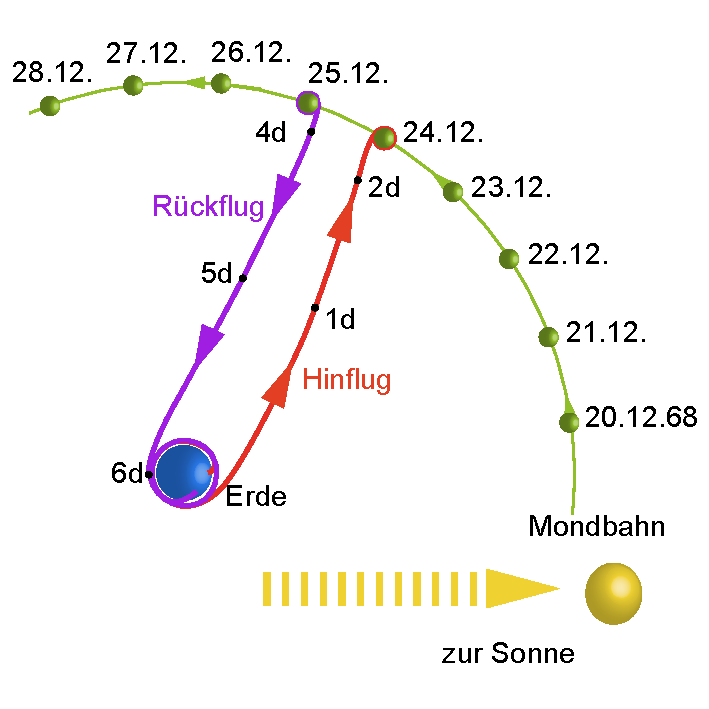
\includegraphics[width=0.5\textwidth]{Apollo8_Bahn.pdf}}
\hspace{\fill}
\rightfigure{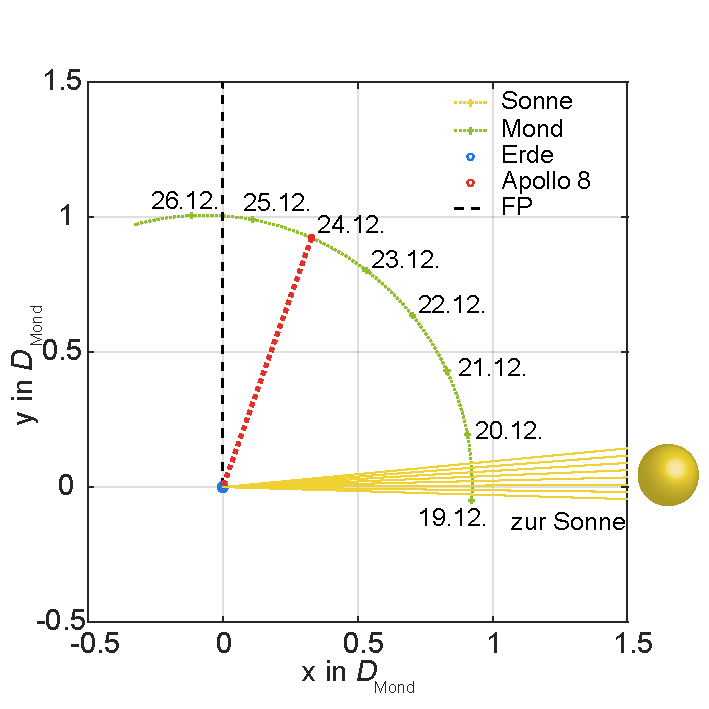
\includegraphics[width=0.5\textwidth]{KonstellationSEMA.pdf}}
\leftcaption[Bahn von Apollo 8.]{Bahn von Apollo 8. \\(Copyright NASA)}\label{abb:hm_Apollo8_Bahn}
\rightcaption[Konstellation von Sonne, Erde, Mond und Apollo 8 am 24.12.1968.]{Berechnete Konstellation von Sonne, Erde, Mond und Apollo 8 am 24.12.1968 um 16:38 UT} \label{abb:hm_EarthRise_calc}
\end{minipage}
\end{figure}
\textcolor{blue} {$\rightarrow$ zur} \probref{hm_erdaufgang_von_apollo}.\\
\noindent\rule[1ex]{\textwidth}{0.5pt} \newpage

%-----------------------------------------------------------------------------------------------------------

\begin{sol}{prob:hm_Analemma_Mars}\label{lsg:hm_Analemma_Mars} %�bung22
\textbf{Zeitgleichung und Analemmas auf anderen Planeten} \\

Wir wollen zun�chst eine sehr einfache Berechnung zeigen, die die Form der Analemmas richtig wider gibt, allerdings keine zeitliche Entwicklung zeigt, da die Kepler-Gleichung nicht gel�st wird.
Man startet dazu mit der exzentrischen Anomalie $E$ und betrachtet ein ganzes planetarisches Jahr, von dem man wei�, dass $E = 0 \ldots 360 \degree$ ist.
Mit Formel \eqref{eq:hm_nu(t)_alternativ}
\begin{equation*}
	\tan \lk \frac{\upsilon_\text{P}}{2} \rk = \sqrt{\frac{1+e_\text{P}}{1-e_\text{P}}}\,\tan\lk\frac{E}{2}\rk~
\end{equation*}
berechnet man die wahre Anomalie $\upsilon_\text{P} (E)$ des Planeten P.
Aus dieser bestimmt man �ber \eqref{eq:hm_ekl_laenge_erde1} und \eqref{eq:hm_lambda_S(T)} die L�ngen der wahren und mittleren Sonne
\begin{equation*}
L_\text{P,\astrosun} = \upsilon_\text{P} +  L_\text{P,Per}\,,~~~ L_\text{P,M} = M_\text{P} +  L_\text{P,Per} \,.
\end{equation*}
Dazu braucht man die planetozentrische L�nge des Perihels.
Das ist der Winkelabstand des Perihels vom planetaren Fr�hlingspunkt, der sich wiederum als Schnittpunkt der �quatorebene des Planeten mit der Bahnebene des Planeten ergibt.

	\begin{figure}[H]
	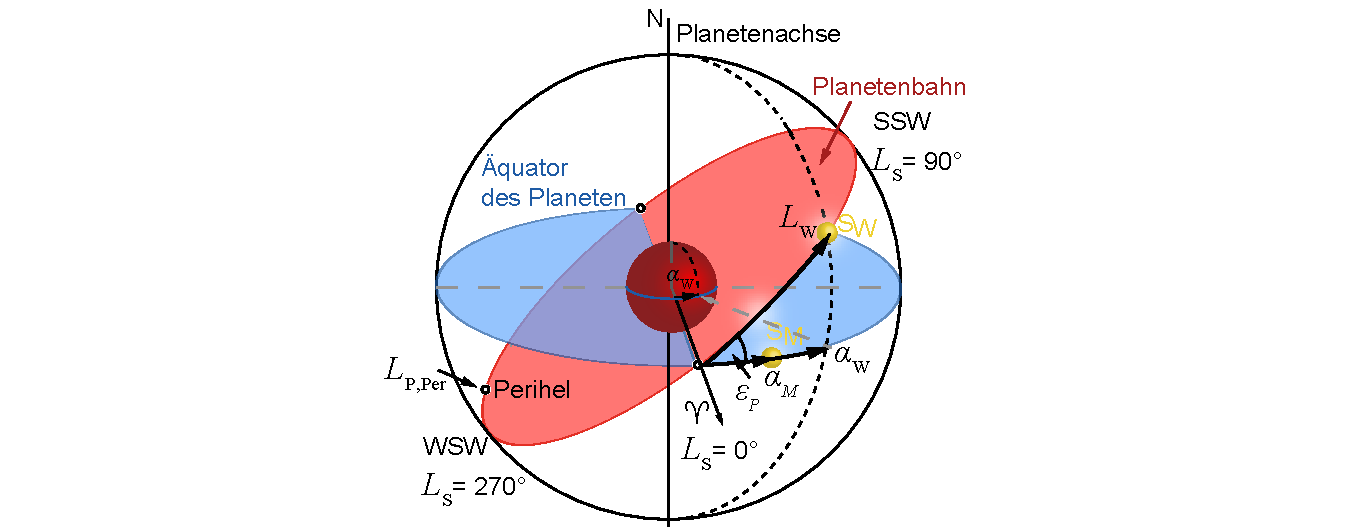
\includegraphics[width=0.8\textwidth]{ZGLGeometrie.pdf}%
	\caption{Ableitung der planetaren Sonnenkoordinaten}%
	\label{abb:hm_ZGLGeometrie_lsg}%
	\end{figure}

Wir betrachten dazu \figref{hm_ZGLGeometrie_lsg}, die der \figref{hm_wahre_sonne_geoz} aus \kap{hm_naeherungsformeln_sonne} f�r die Erde entspricht.
Wie dort dargestellt, geht es auch hier um die Anwendung von Gleichung \eqref{eq:hm_tau_ZGL_C}.
Hier m�ssen wir nun anstelle der ekliptikalen L�nge $\lambda_\text{\astrosun}$ und der geozentrischen Rektaszension $\alpha_\text{\astrosun}$ die planetozentrische L�nge $L_\text{P,\astrosun}$\index{L�nge!planetozentrische} und die planetozentrische Rektaszension \index{Rektaszension!planetozentrische} \index{Rektaszension!planetare} $\alpha_\text{P,\astrosun}$ verwenden.
Mit dem Begriff \emph{planetare} oder \emph{planetozentrische} Rektaszension ist analog zur "`normalen"' \emph{geozentrischen} Rektaszension ein Winkel gemeint, der entlang des planetaren �quators vom \emph{planetaren}(!) Fr�hlingspunkt zum Fusspunkt der wahren Sonne aus gemessen wird. 
Die (planetare) Rektaszension ergibt sich aus der entsprechenden Umrechnungsformel vom planeto-ekliptikalen System in das planeto-�quatoriale KOS (Tab. \ref{tab:hm_astro_KOS}):
\begin{equation*}
\tan\alpha_\text{P,\astrosun} = \cos\epsilon_\text{P} \, \tan{L_\text{P,\astrosun}} ~~\text{bzw.}~~~ \alpha_\text{P,M} = L_\text{P,M}~,
\end{equation*}
worin $\epsilon_\text{P}$ die Polneigung des jeweiligen Planeten relativ zu seiner Bahn ist.
Damit ergibt sich der Stundenwinkel nach \eqref{eq:hm_tau_ZGL_C} zu $\tau = \alpha_\text{M} - \alpha_\text{\astrosun}$.
Die Deklination der wahren Sonne berechnet sich ebenfalls aus Tabelle \ref{tab:hm_astro_KOS} zu:
\begin{equation*}
\sin\delta_\text{\astrosun} = \sin\epsilon_\text{P} \, \sin{L_\text{P,\astrosun}} ~, 
\end{equation*}
womit wir alle Berechnungsdaten f�r die Analemmas der Planeten haben.

\begin{figure}[H]
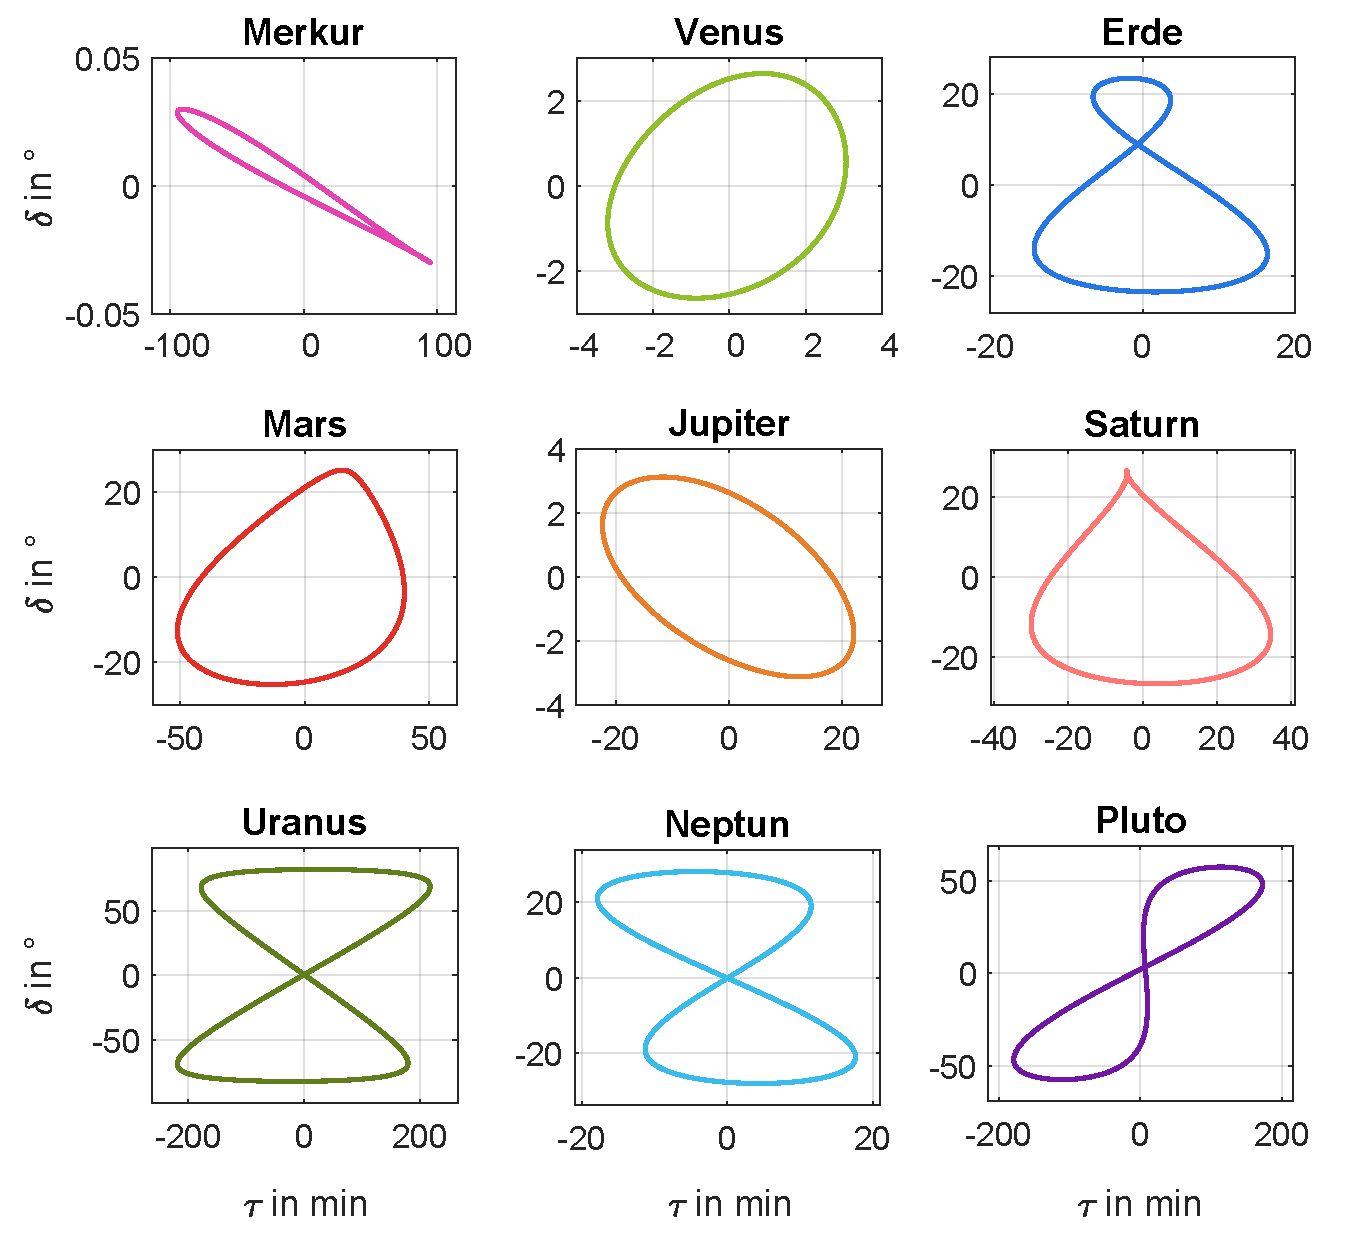
\includegraphics[width=\textwidth]{AnalemmaPlaneten.pdf}
\caption{Analemma f�r die Planeten Merkur bis Pluto.}\label{abb:hm_analemma_planeten_lsg}
\end{figure}
Details der Berechnung sind in \mlhmref{Analemma03.m} zu finden.
Das Ergebnis der Berechnung l�sst sich zusammenfassen, wobei wir den Index P f�r den Planeten weglassen, aber noch einmal darauf hinweisen, dass hier die $L_\text{Per}$ nicht den in Tabelle \ref{tab:hm_bahnparameter} gelisteten heliozentrisch-ekliptikalen L�ngen des Perihels entsprechen, sondern den planetozentrischen $L_\text{P,Per}$.
\begin{align*}
    \tau_\text{ZGL}(E) &= M + L_\text{Per} - \arctan\left\{\cos\epsilon\:\tan\left[L_\text{Per} +  2 \arctan\lk\sqrt{\frac{1+e}{1-e}} \tan\lk \frac{E}{2} \rk \rk \right] \right\} ~,\\
    \delta(E) &= \arcsin\left\{\sin\epsilon \sin\left[L_\text{Per} + 2 \arctan\lk \sqrt{\frac{1+e}{1-e}} \tan\lk \frac{E}{2} \rk \rk \right] \right\}
\end{align*}
Die entsprechenden Rechnungen haben wir im \mscr~\mlhmref{AnalemmaAnomalie.m} durchgef�hrt und sind in \figref{hm_analemma_planeten_lsg} gezeigt.
Wir geben die planetozentrischen L�ngen des Perihels ebenfalls im \mscr~an.
Wir sehen im Ergebnis, dass nur auf einigen Planeten  das Analemma als die von der Erde bekannten Figur der "`Acht"' erscheint, auf anderen Planeten kommt es wegen des unterschiedlichen Zusammenspiels der Parameter Achsneigung und Exzentrizit�t zu anderen Bildern.
Wenn einer der Bahnparameter dominiert, wie z.B. die Exzentrizit�t beim Mars, dann �hnelt das Analemma eher einer Tr�ne (siehe \figref{hm_analemma_planeten_lsg}), wenn hingegen die Achsneigung sehr klein ist, wie beim Jupiter (nur $3\degree$) wird die Figur �hnlich einer Ellipse.
Man beachte daher die ausgepr�gte Form und Breite bei Planetenbahnen mit gro�er Exzentrizit�t (Merkur, Mars, Saturn), die verschwindende Form der "`Acht"' bei geringer Polneigung (Merkur, Venus, Jupiter) bzw. das �berwiegen der Exzentrizit�t �ber die Polneigung (Mars, Saturn).\\
Wir wollen uns nun auch der Zeitgleichung zuwenden und m�ssen dazu die L�sung der Kepler-Gleichung f�r den jeweiligen Planeten ber�cksichtigen.
Wir skizzieren dazu zwei alternative Methoden. \\

\emph{Methode 1 (nach Allison\footnote{Die Rechnungen erfolgen analog den Betrachtungen in Kapitel \ref{kap:zeitgleichung} und sind in den \mscren zur �bung im Detail beschrieben. Wir verweisen ferner auf die Darstellungen in \cite{Allison2000} und \cite{Goddard2019}, in denen die Rechnungen ausf�hrlich f�r den Mars hergeleitet wurden. Wir haben in der �bung das Vorgehen f�r alle Planeten verallgemeinert.})}

Die Rotation des Planeten muss man zun�chst nicht ber�cksichtigen.
Man muss aber wiederum die Lage der Planetenbahn relativ zum planetaren �quator kennen oder m.a.W. die Richtung der Planetenrotationsachse relativ zu seiner Bahnebene.
Wir verweisen wieder auf die \figref{hm_ZGLGeometrie_lsg}, dann besteht die Aufgabe in Folgendem:
\begin{enumerate} 
	\item 	Es m�ssen die Keplerschen Elemente der Planetenbahn (bzw. der vom Planeten aus gesehenen Sonnenbahn) relativ zum planetaren �quator und Fr�hlingspunkt ausgedr�ckt werden.
          Bekannt sind dabei ja zun�chst nur die Bahnelemente bezogen auf die (Erd-)Ekliptik und den Erdfr�hlingspunkt.
          Halbachse und Exzentrizit�t �ndern sich nicht, ebenso bleibt die mittlere Anomalie unver�ndert.
          Die anderen Bahnelemente m�ssen jedoch transformiert werden.
	\item 	Mit der Inklination $i$, der L�nge des Knotens $\Omega$, dem Argument des Perihels $\omega$ und der Richtung der Rotationsachse des Planeten (deren Richtungswerte\footnote{Mit Richtung der Rotationsachse meinen wir die geozentrische Rektaszension und Deklination des Punktes an der Himmelskugel auf den die Rotationsachse zeigt.} $\alpha_0, \delta_0$ man aus der Literatur entnimmt) muss man nun die Lage des planetaren Fr�hlingspunktes (PFP) \index{Fr�hlingspunkt!planetarer} auf dem planetaren �quator berechnen (siehe \figref{hm_ZGLNullmeridian_lsg}) und daraus den Winkel $L_{\text{P,Per}}$ zwischen planetarem Fr�hlingspunkt und Perihelion der Planetenbahn.
	\item 	Am einfachsten geht das mittels Rotationsmatrizen f�r die kartesischen Vektoren normal zu den einzelnen Ebenen und entlang der jeweiligen Knotenlinien. 
	\item 	Mit diesen Gr��en kann dann die planetare Zeitgleichung, die der ekliptikalen ZGL nach \eqref{eq:hm_tau_ZGL_C} bzw. \eqref{eq:hm_tau_ZGL_C1} entspricht, berechnet werden:
		\[\tau_\text{ZGL, P} = (L_\text{P,\astrosun}-\alpha_\text{P,\astrosun}) + \mathcal{C} \\
	\]
	\item Mit der Deklination $\delta_\text{P,\astrosun}$, die wir aus der planetozentrischen L�nge der Sonne und der Achsneigung analog \eqref{eq:hm_alpha_s_delta_s} berechnen, erstellen wir dann das Analemma.
\end{enumerate}

\begin{figure}[H]
	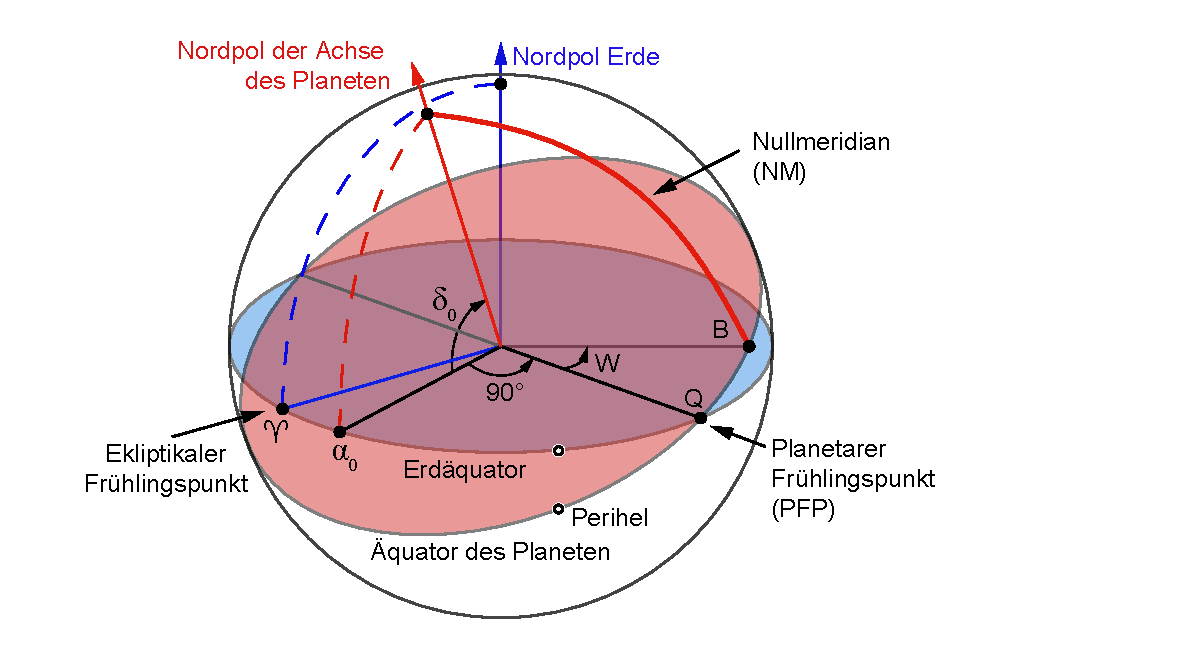
\includegraphics[width=\textwidth]{ZGLNullmeridian.pdf}%
	\caption[Planetarer Fr�hlingspunkt und Nullmeridian.]{Planetarer Fr�hlingspunkt (PFP) und Nullmeridian (NM).}%
	\label{abb:hm_ZGLNullmeridian_lsg}%
\end{figure}

Die entsprechenden Rechnungen haben wir im \mscr~\mlhmref{ZGLAnalemma.m} durchgef�hrt.

\begin{figure}[H]
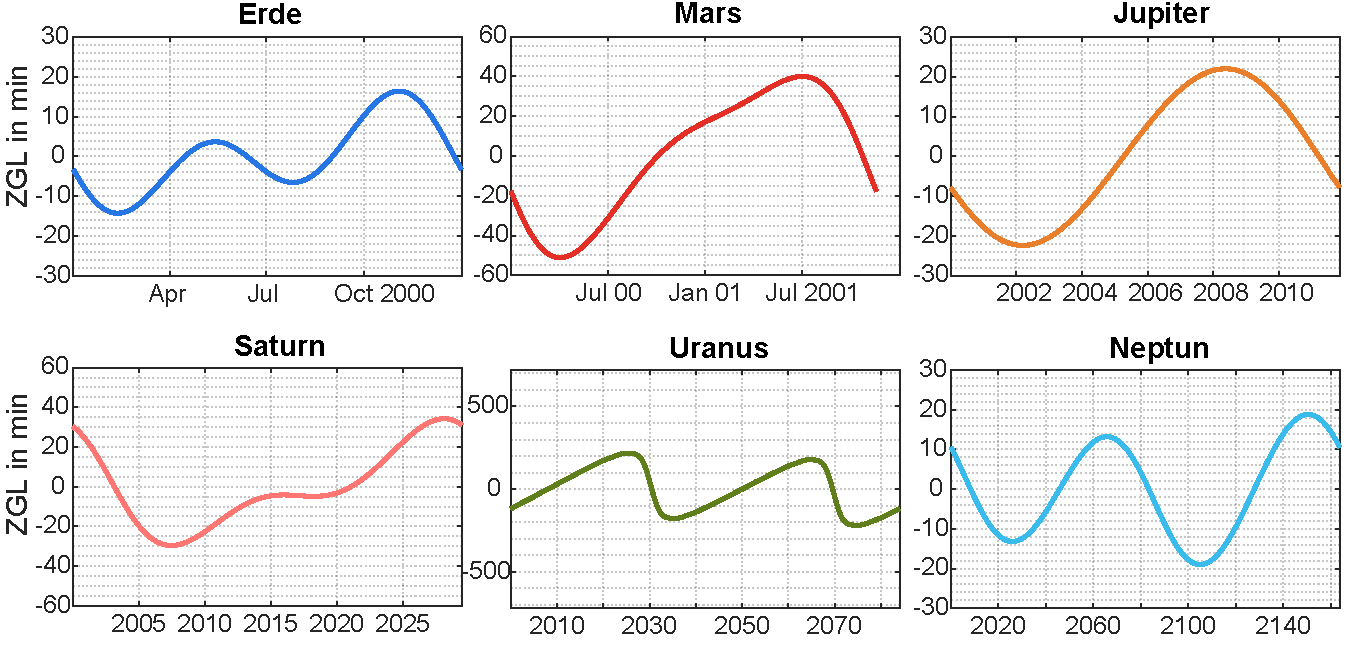
\includegraphics[width=\textwidth]{ZGLAnalemma.pdf}
\caption{Zeitgleichung f�r einige Planeten.}\label{abb:hm_zgl_planeten_lsg}
\end{figure}

Die Ergebnisse der Zeitgleichungsrechnung sind in \ref{abb:hm_zgl_planeten_lsg} dargestellt, die Analemmas stimmen erwartungsgem�� mit denen von \ref{abb:hm_analemma_planeten_lsg} �berein.
Wir wollen hier nochmals auf die Besonderheit des Uranus verweisen.
Der Uranus braucht etwa 84 Jahre, bis er die Sonne einmal umrundet hat.
Dabei dauert ein Tag auf dem Uranus nur 17 Stunden und 14 Minuten.
Da seine Polachse fast in der Bahnebene liegt rollt er quasi auf seiner Bahnebene um die Sonne, wobei f�r fast ein halbes Jahr der Nordpol, das andere Halbjahr der S�dpol zur Sonne zeigt.
Die ZGL und damit Jahreszeiten sind aus diesem Grund ziemlich "`verr�ckt"'.
Es bleibt auf dem Uranus im Sommer 42 Erden-Jahre lang st�ndig hell und wird dann abrupt dunkel.
Das Analemma zeigt das sehr sch�n.\\

\emph{Methode 2 (nach Montenbruck\footnote{Mit der Methode ist dann auch die Position jedes anderen Himmelsk�rpers im KOS des Planeten berechenbar. F�r Details verweisen wir auf \cite{Montenbruck1999, Haase2013}.})} 

Auch hier wollen wir die Methodik kurz skizzieren.
Man berechnet (numerisch) f�r einen Punkt auf der Oberfl�che des Planeten (gegeben durch die planetographischen Koordinaten $\varphi_\text{P}$ und $\lambda_\text{P}$) die planetare Rektaszension und Deklination der Sonne im planetozentrischem �quatorialsystem f�r den Verlauf eines tropischen Jahres.
Aus diesen Koordinaten lassen sich dann v�llig analog zur Erde bei Festlegung einer geeigneten Planeten-Nullzeit (z.B. Nullmeridian NM in \figref{hm_ZGLNullmeridian_lsg}) die Aufg�nge und Unterg�nge der Sonne und nat�rlich auch den Meridiandurchgang f�r jeden Ort $\varphi_\text{P}$, $\lambda_\text{P}$ des Planeten bestimmen.
Zusammengefasst ist das Vorgehen also wie folgt:
\begin{enumerate} 
	\item Ausgehend von der heliozentrischen Position des Planeten berechnet man die planetozentrischen Koordinaten $\alpha_\text{P,\astrosun}$  und $\delta_\text{P,\astrosun}$ der wahren Sonne im Verlauf eines tropischen Jahres.
	\item Die mittlere Sonne berechnen wir �ber die mittlere Anomalie.
          Alternativ k�nnten wir auch aus der Kenntnis der Rotationsperiode des Planeten eine Planetensternzeit $\theta_\text{P}$ berechnen, wobei sich die Zeitgleichung dann entweder �ber \eqref{eq:hm_tau_ZGL_C} bzw. $\tau_\text{ZGL} = \theta_\text{P} - \alpha_\text{P,\astrosun}$ berechnet. 
	\item Mit der Deklination $\delta_\text{P,\astrosun}$ aus der planetozentrischen Breite der wahren Sonne erstellen wir dann das Analemma.
\end{enumerate}

Die entsprechenden Rechnungen haben wir im \mscr~\mlhmref{ZGLAnalemmaKepler.m} bzw. f�r alle Planeten hinterlegt.
Auch hier stimmen die Analemmas erwartungsgem�� mit denen von \figref{hm_analemma_planeten_lsg} und die Zeitgleichungen mit denen von \figref{hm_zgl_planeten_lsg} �berein. \\

Eine sch�ne Erweiterung der Methodik ist die Anwendung auf die Berechnung eines Analemmas des Mondes (von der Erde aus betrachtet) \bzw eines Analemmas der Sonne vom Mond aus betrachtet.
In den \matlab{}-Skripten \mlhmref{ZGLAnalemma.m}, \mlhmref{ZGLAnalemmaKepler.m} und \mlhmref{AnalemmaAnomalie.m} sind die Rechnungen dazu detailliert hinterlegt.

\medskip \end{sol}
\textcolor{blue} {$\rightarrow$ zur} \probref{hm_Analemma_Mars}.\\
\noindent\rule[1ex]{\textwidth}{0.5pt} \newpage

%-----------------------------------------------------------------------------------------------------------

\begin{sol}{prob:hm_sonnenaufgang_mars}\label{lsg:hm_sonnenaufgang_mars} %�bung23
\textbf{Sonnenaufgang Mars} \\ \\
In \probref{hm_Analemma_Mars} haben wir die Zeitgleichung und das Analemma f�r den Mars hergeleitet.
Wir haben dort ebenfalls eine Referenz f�r die Zeitmessung auf den Mars und einen Bezug zur UTC hergestellt.
Wir k�nnen selbstverst�ndlich auch andere Referenzzeitpunkte w�hlen, wie \zb die Landezeit einer Marssonde. 
Wir wollen nun auf Basis der aktuellen NASA Konventionen die Sonnenaufgangsberechnung durchf�hren und benutzen dabei neben den Ergebnissen von \probref{hm_Analemma_Mars} auch den Algorithmus der NASA \cite{Goddard2019}.
Die detaillierten Rechnungen sind i\mscr{} \mlhmref{OlympusMons.m} hinterlegt, das Ergebnis der Rechnungen ist in \figref{hm_Mars_Sunrise_lsg} zu sehen.
Wie schon beim Analemma in L�sung \ref{lsg:hm_Analemma_Mars} erkennt man auch hier deutlich die unterschiedlich langen Jahreszeiten (als Folge der gro�en Exzentrizit�t) und auch, da der Beobachtungsort nahe des Mars-�quators liegt, dass die jahreszeitlichen Schwankungen im wesentlichen die ZGL widerspiegeln.\\
\begin{figure}[H]
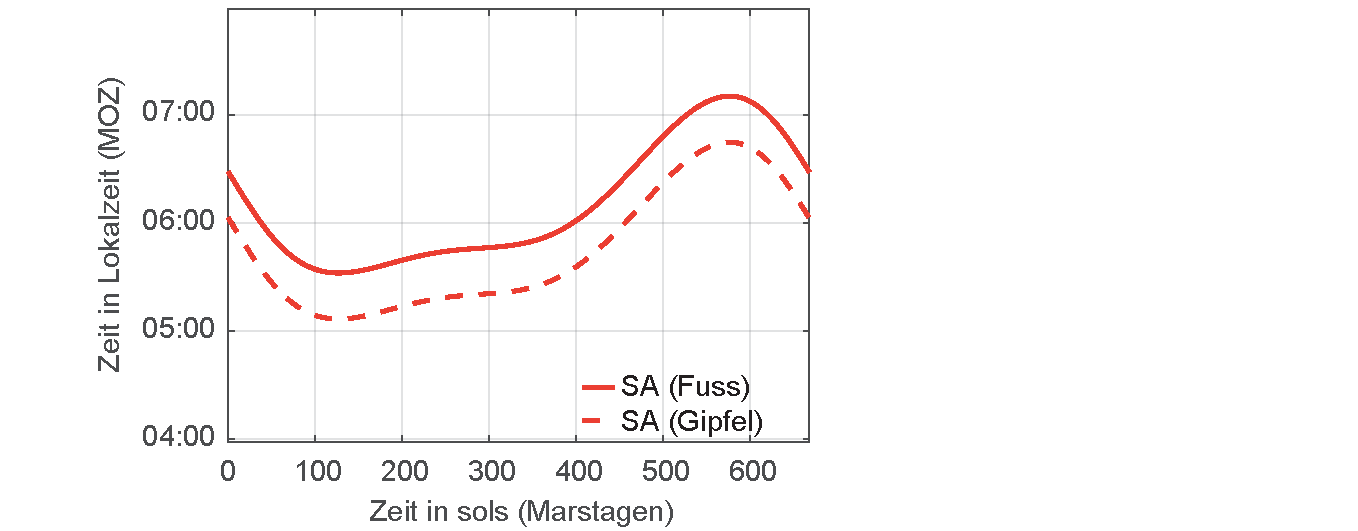
\includegraphics[width=\columnwidth]{OlympusMons.pdf}%
\caption[Sonnenaufgangszeiten auf dem Mars.]{Sonnenaufgangszeiten auf dem Mars am Fu� und auf dem Gipfel des Olympus Mons im Verlauf eines Mars-Jahres. Das Mars-Sommer Halbjahr erstreckt etwa von Tag 1 bis Tag 450 und damit wesentlich l�nger als das Winterhalbjahr.}%
\label{abb:hm_Mars_Sunrise_lsg}%
\end{figure}
\medskip \end{sol}
\textcolor{blue} {$\rightarrow$ zur} \probref{hm_sonnenaufgang_mars}.\\
\noindent\rule[1ex]{\textwidth}{0.5pt} \newpage

%-----------------------------------------------------------------------------------------------------------
\newpage
%%%-----------------------------------------------------------------------------------------------------------
\subsection{�bungen zu Monden, Kometen und Asteroiden}

\medskip

\begin{sol}{prob:hm_MondbahnHelioz}\label{lsg:hm_MondbahnHelioz} %�bung24
\textbf{Heliozentrische Mondbahn} \\

Heliozentrisch betrachtet l�uft der Mond um die Sonne und wird dabei von der Erde ein wenig abgelenkt. Die Mondbahn ist aber stets
zur Sonne hin gekr�mmt, und die St�rke dieser Kr�mmung �ndert
sich im Lauf eines Monats nur m��ig, da die Gravitationskraft
der Sonne am Ort des Mondes zu jeder Zeit deutlich
gr��er als diejenige der Erde ist, was man leicht nachrechnen kann. 
Geozentrisch ist es aber ebenfalls richtig zu sagen,
dass der Mond um die Erde l�uft und dabei von der Sonne
gest�rt wird, was zu seiner komplexen Bahn f�hrt.
Es gilt aber auch hier, dass die Schwerkraft
der Erde am Ort des Mondes zu jedem Zeitpunkt deutlich gr��er ist als
die Gezeitenkraft der Sonne auf das Erde-Mond-System ist, denn sonst w�rde dieses ja auseinander gerissen werden (siehe \kap{hm_gezeiten}). Man kann auch sagen, dass nur die Differenz der solaren Einfl�sse auf Erde und Mond sich als St�rung der
geozentrischen Mondbahn auswirkt.\\
Man kann sich nun recht einfach �berlegen, unter welchen Bedingungen schleifen- oder wellenf�rmige Mondbahnen zustande kommen k�nnen.
Wir wollen vereinfachend annehmen, dass die Planetenbahn und zugeh�rige Mondbahn ann�hernd koplanar und zirkular sind, also
gegeneinander nur wenig geneigt und wenig exzentrisch sind. 
Aus der Gravitationsbeschleunigung und dem dritten Keplerschen Gesetz findet man
folgende Beziehungen:
\begin{itemize}
\item Fall 1: Konvexe Bahn (wie Erdmond) : $T_\text{M}^2/T_\text{P}^2 > a_\text{M}/a_\text{P}$
\item Fall 2: Schleifenbahn : $T_\text{M}/T_\text{P} < a_\text{M}/a_\text{P}$
\item Fall 3: Wellenbahn : $T_\text{M}/T_\text{P} > a_\text{M}/a_\text{P} > T_\text{M}^2/T_\text{P}^2$
\end{itemize}
Hierin sind $T_\text{M},\, T_\text{P}$ die Umlaufzeiten von Mond und Planet und $a_\text{M},\, a_\text{P}$ die entsprechenden Radien der Bahnen.
Die erste Bedingung besagt, dass die
Gravitationsbeschleunigung des Mondes
durch den Planeten kleiner ist als diejenige
durch die Sonne, was beim Erdmond sicher erf�llt ist. Die zweite Bedingung
besagt, dass die Umlaufgeschwindigkeit
des Mondes um den Planeten gr��er
ist als die Geschwindigkeit des Planeten
um die Sonne. Dies ist beim Erde Mond System nicht erf�llt. Wegen $a_\text{M} \ll a_\text{P}$ ergibt sich deshalb beim Mond der Erde nur eine geringf�gig ausgepr�gte Wellenbahn 
(\figref{hm_mondbahn_lsg02}).\\
Wir wollen das in einer einfachen, komplanaren Modellrechnung zeigen und schreiben: 
\begin{align}
\begin{split}
    x_\text{M} &= a_\text{P}\,\cos\Omega_\text{P} \,t + a_\text{M}\,\cos\omega_\text{M}\,t \\
    y_\text{M} &= a_\text{P}\,\sin\Omega_\text{P} \,t + a_\text{M}\,\sin\omega_\text{M}\,t
\end{split} \label{eq:hm_lsgmondb01}
\end{align}
$t=0$ wurde hier so gew�hlt, dass $\vec{r}\lk 0\rk = \vec{r}_\text{M,0}  =  \lk x_\text{M},y_\text{M} \rk= \lk a_\text{P} + a_\text{M},0\rk $ ist. \\
Unser Kurvenparameter ist die Zeit $t$. Wir wollen den Kr�mmungsradius $\varrho$ und die Konvexit�t $\eta = \D^2 y/\D x^2$ als Funktion der Zeit berechnen. Gilt $\eta > 0$ ist die Bahn konvex, f�r Zeitbereiche in denen $\eta <0$ ist die Bahn konkav. \\
In Parameterdarstellung ist der Kr�mmungsradius $\varrho$ gegeben durch:
\begin{align}
    \varrho = \Bigg|\frac{\lk \dot{x}^2+ \dot{y}^2\rk^\frac{3}{2}}{\lk \dot{x}\ddot{y} -\ddot{x}\dot{y}\rk}\Bigg| = \Bigg|\frac{\lk \dot{x}^2+ \dot{y}^2\rk^\frac{3}{2}}{\det\lk \dot{\vec{r}},\ddot{\vec{r}}\rk}\Bigg| \label{eq:hm_lsgmondb02} \,. 
\end{align}
\begin{table}[h!]
    \centering
    \begin{tabular}{l|rcrcr}
         & $T_\text{M}{}^2/T_\text{P}{}^2$ & & $a_\text{M}/a_\text{P}$&&$T_\text{M}/T_\text{P}$\\
         \rule{0pt}{1pt}& & & & &  \\
         \hline
         \rule{0pt}{1pt}& & & & &  \\
         \rule{0pt}{6pt}Fall 1~~~ & $~0.25$ & $>$ & $0.1$ & & $0.5$ \\
         \rule{0pt}{6pt}Fall 2~~~ & $~0.0025$ & & $0.1$ & $>$& $0.05$ \\
         \rule{0pt}{6pt}Fall 3~~~ & $~0.01$ & $<$ & $0.1$ & $\leq$& $0.1$ 
    \end{tabular}
\end{table}\\
Man erkennt deutlich, dass je nach Fall die Schleifenbahn, eine Art Epizykloide auf einem Kreis mit dem Radius $a_\text{P}-a_\text{M}$ oder eben eine sehr flache Welle darstellt. Das Erde-Mond System f�llt in die Kategorie des Fall 1 mit $a_\text{P} \gg a_\text{M}$.\\
F�r stark geneigte Bahnen ergben sich durch notwendige Ber�cksichtigung der Bahnneigung etwas durch die Inklination
$\cos i$ modifizierte Beziehungen.\\
Die numerische Berechnung der 3 Beispiele ist mit entsprechenden Modellparametern sehr einfach zu realisieren und im \mscr{} \mlhmref{Mondbahn01.m} f�r koplanare kreisf�rmige Bahnen ausgef�hrt. Im \mscr{} \mlhmref{Mondbahn02.m} ist auch die heliozentrische Mondbahn aus den genauen Ephemeriden berechnet (\figref{hm_mondbahn_lsg03}).

\begin{figure}[H]
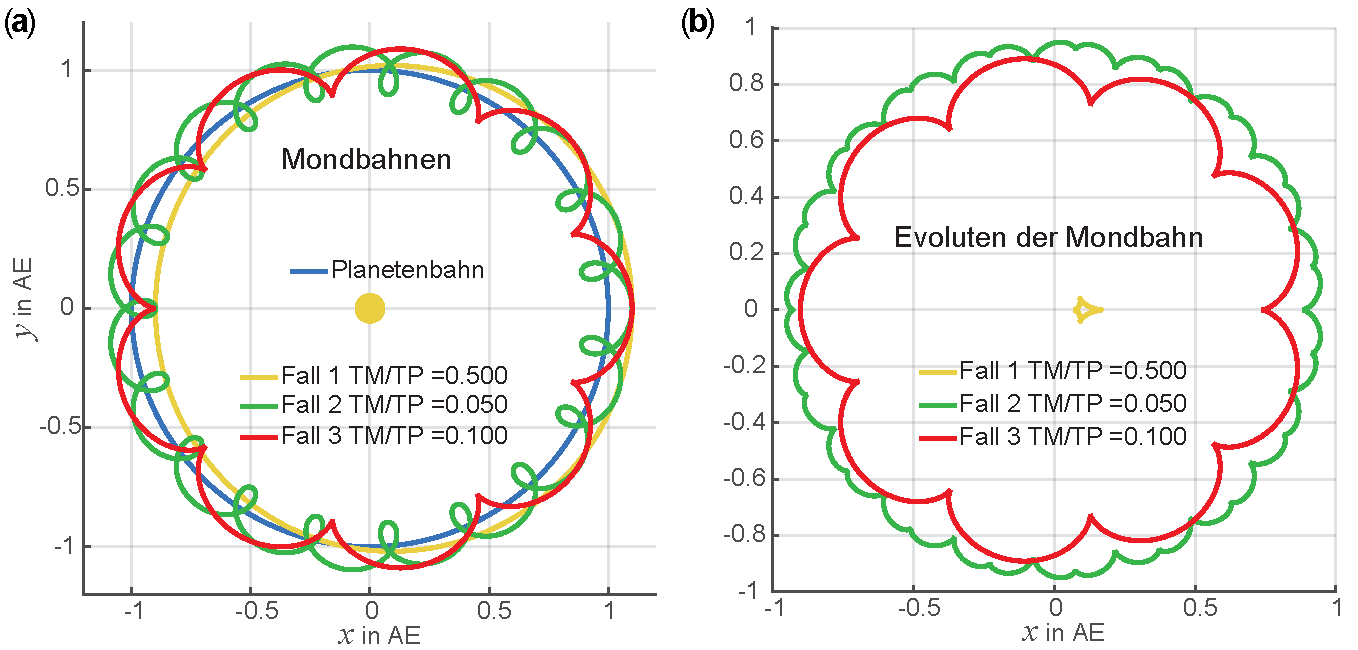
\includegraphics[width=\textwidth]{MondbahnHelioz3.pdf}
\caption[Heliozentrische Mondbahnen f�r koplanare, kreisf�rmige Bahnen.]{Heliozentrische Mondbahnen f�r koplanare, kreisf�rmige Bahnen Planet und Mond. \fa Mondbahnen \fb Lage der Mittelpunkte des lokalen Kr�mmungskreises (Evolute der Mondbahn). Das Verh�ltnis der Bahnradien von Mondbahn zu Planetenbahn wurde fest zu 0.1 angenommen, variiert wurden die Umlaufzeiten \bzw nach dem 3. Keplerschen Gesetz die Massen von Zentralk�rper und Planet.}\label{abb:hm_mondbahn_lsg01}
\end{figure}

\begin{figure}[H]
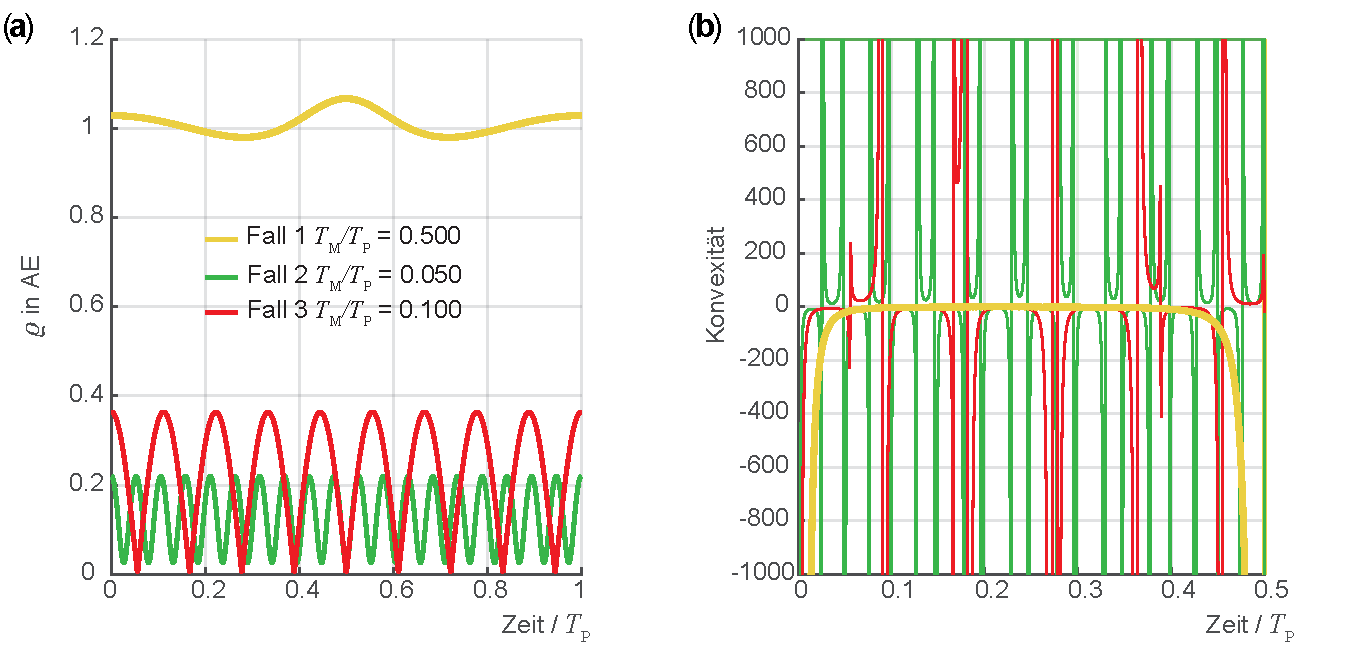
\includegraphics[width=\textwidth]{MondbahnHelioz4.pdf}
\caption[Kr�mmungsradius und Konvexit�t heliozentrischer Mondbahnen.]{Heliozentrische Mondbahnen f�r koplanare, kreisf�rmige Bahnen Planet und Mond. \fa Kr�mmungsradius \fb Konvexit�t. Das Verh�ltnis der Bahnradien von Mondbahn zu Planetenbahn wurde fest zu 0.1 angenommen, variiert wurden die Umlaufzeiten \bzw nach dem 3. Keplerschen Gesetz die Massen von Zentralk�rper und Planet.}\label{abb:hm_mondbahn_lsg02}
\end{figure}

\begin{figure}[H]
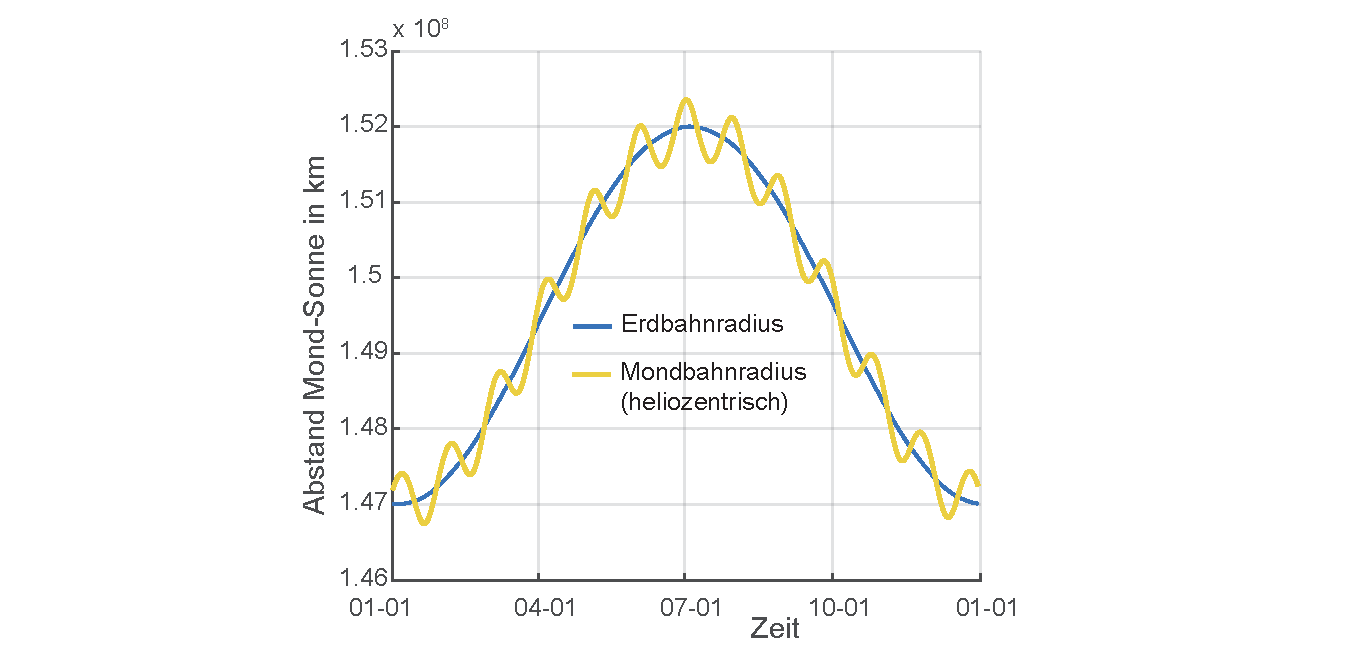
\includegraphics[width=\textwidth]{MondbahnHelioz2.pdf}
\caption{Heliozentrische Mondbahn aus den Ephemeriden berechnet}\label{abb:hm_mondbahn_lsg03}
\end{figure}


\medskip \end{sol}
\textcolor{blue} {$\rightarrow$ zur} \probref{hm_MondbahnHelioz}.\\
\noindent\rule[1ex]{\textwidth}{0.5pt} \newpage



%-----------------------------------------------------------------------------------------------------------

\begin{sol}{prob:hm_kometen_asteroiden} \label{lsg:hm_kometen_asteroiden} %�bung25
\textbf{Kometen und Asteroiden} \\ \\
Die Rechnungen sind im Detail in den einzelnen \mscren zu den Kometen- und Asteroidenbahnen \ua \mlhmref{AsteroidenBahnen.m} und \mlhmref{AsteroidenZeit.m} ausgef�hrt. Eine Beispielrechnung ist als Bild angef�gt. \\

\begin{figure}[H]
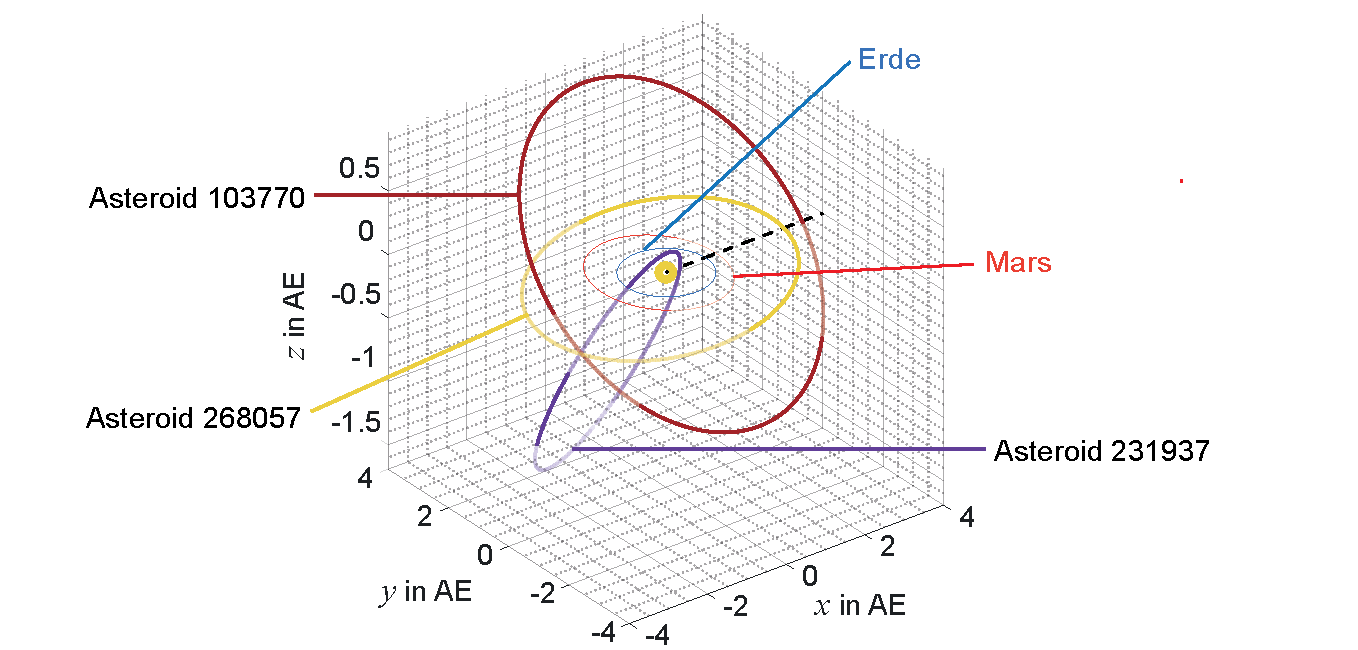
\includegraphics[width=\textwidth]{AsteroidenbahnenBeispiele.pdf}
\caption{Beispiele vo Asteroidenbahnen}\label{abb:hm_AsteroidenbahnenBeispiele}
\end{figure}

\medskip \end{sol}
\textcolor{blue} {$\rightarrow$ zur} \probref{hm_kometen_asteroiden}.\\
\noindent\rule[1ex]{\textwidth}{0.5pt} \newpage


%-----------------------------------------------------------------------------------------------------------


\begin{sol}{prob:hm_verweildauer_komet_erdbahn}\label{lsg:hm_verweildauer_komet_erdbahn} %�bung26
\textbf{Kometen und Meteoriten} \\
\begin{enumerate}[(a)]
	\item Wir vereinfachen zun�chst das Problem und nehmen an, dass die Kometenbahn in der Ekliptik liegt und dass diese in der N�he ihres Perihels als Parabel beschrieben werden kann.
          Somit ist die Exzentrizit�t $e\!=\!1$ und \eqref{eq:hm_kegelschnitt} vereinfacht sich zu
\begin{equation}
r = \frac{p}{1+\cos\upsilon}~~\text{mit}~~p=\frac{L^2}{\mu_\text{G}} ~~.\label{eq:hm_hmlsg_24_1}
\end{equation}
Der minimale Abstand ist demnach $r_\text{min}\!=\!q\!=\!p/2\!=\!L^2/(2\mu_\text{G})$.
F�r die spezifische Energie des Kometen gilt nach \eqref{eq:hm_total_energy} im Fall von Parabeln
\begin{equation}
H = \frac{1}{2}\dot{r}^2 + \frac{L^2}{2r^2} + U(r) ~~. \label{eq:hm_hmlsg_24_2}
\end{equation}
Am Perihel mit Abstand $r_\text{min} = q$ ist die Radialgeschwindigkeit $\dot{r}\!=\!0$, so dass
\begin{align*}
	\frac{L^2}{2r_\text{min}^2} &= -U(r_\text{min}) = \frac{\mu_\text{G}}{r_\text{min}} = \frac{\mu_\text{G}}{q} \\
	\Rightarrow L &= \sqrt{2\mu_\text{G}\,q}~~.
\end{align*}
Wir dr�cken nun den Perihelabstand als $q\!=\!r_\text{min}\!=\!ka_\text{\earth}\!=\! k\, 1\text{AE}$ mit $0\!<\!k\!<\!1$ aus.
Mit $\D t\!=\!\D r/\dot{r}$ und $\dot{r}\!=\!\sqrt{2[-U(r)-L^2/(2r^2)]}$ folgt aus \eqref{eq:hm_hmlsg_24_2}
\begin{align*}
	t-t_0 &= \int\limits_{q}^{r=a_\text{\earth}} \frac{r}{\sqrt{2\mu_\text{G}r-L^2}}\,\D r = \sqrt{\frac{1}{2\mu_\text{G}}} \int\limits_{q}^{r} \frac{r}{\sqrt{r-L^2/2\mu_\text{G}}}\,\D r ~~.\\
\end{align*}
In Integraltafeln finden wir als L�sung f�r das Integral
\begin{equation*}
t-t_0 = \frac{1}{\sqrt{2\mu_\text{G}}}\,\frac{2}{3}\,\sqrt{r-q}\,(2q+r) \bigg|^{a_\text{\earth}}_{q}~~.
\end{equation*}
Die Gesamtaufenthaltsdauer des Kometen innerhalb der Erdbahn, in welcher der Komet gut beobachtet werden kann, ist dann gegeben durch
\begin{align}
	T_\text{ges} &= \frac{2}{\sqrt{2\mu_\text{G}}}\,\frac{2}{3}\,\lek \sqrt{a_\text{\earth}-ka_\text{\earth}} \lk 2ka_\text{\earth} + a_\text{\earth} \rk - \sqrt{q-q} \lk 2ka_\text{\earth} + a_\text{\earth} \rk \rek \\
	 &= \frac{2}{\sqrt{2\mu_\text{G}}}\,\frac{2}{3}\,\sqrt{a_\text{\earth}^3}\,\sqrt{1-k}\,(2k+1) = \frac{4}{3}\,\sqrt{\frac{a_\text{\earth}^3}{2\mu_\text{G}}}\,\sqrt{1+3k-4k^3}~~. \label{eq:hm_verweildauer01}
\end{align}
\begin{figure}[H]
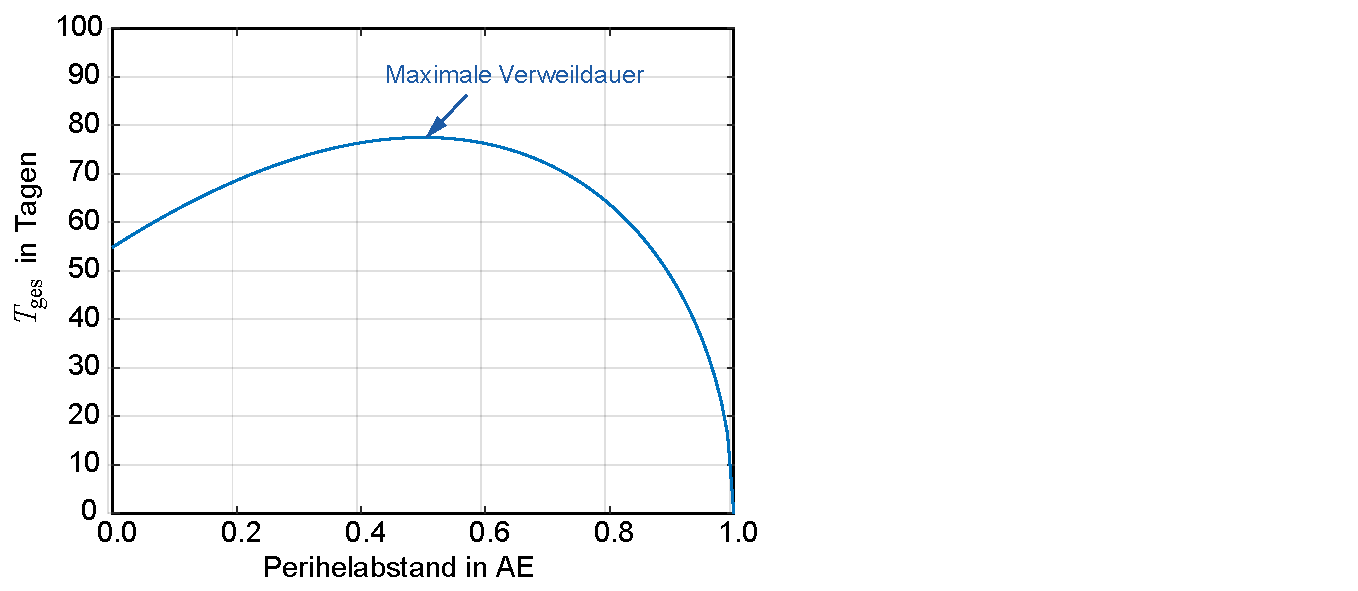
\includegraphics[width=\textwidth]{Verweildauer.pdf}%
\caption[Verweildauer des Kometen in Tagen innerhalb der Erdumlaufbahn.]{Verweildauer des Kometen in Tagen innerhalb der Erdumlaufbahn (Kriterium f�r gute Sichtbarkeit).}%
\label{abb:hm_aufenthaltsdauer_lsg}%
\end{figure}
Die \figref{hm_aufenthaltsdauer_lsg} zeigt die Verweildauer normiert auf die Umlaufdauer der Erde gem��
\begin{equation}
\frac{T_\text{ges}}{2\pi\sqrt{a_\text{\earth}^3/\mu_\text{G}}} = \frac{2}{3}\frac{1}{\sqrt{2}\pi}\,\sqrt{1+3k-4k^3}~~.\label{eq:hm_verweildauer02}
\end{equation}
Man erkennt, dass je kleiner der Perihelabstand ist, desto h�her wird die Geschwindigkeit des Kometen und desto k�rzer seine Aufenthaltsdauer innerhalb der Erdbahn, desto heller leuchtet er aber auch.
Interessant ist auch, dass die maximale Dauer auf etwa 80 Tage begrenzt ist.\\

\item Wir betrachten einen Meteoroiden, der sich im Schwerefeld von Sonne und Erde bewegt (\figref{hm_aufschlaggeschw}):
Wir wollen seine Position zun�chst in einem rotierenden KOS betrachten, das sich mit der Winkelgeschwindigkeit $\omega$ der Erde um Sonne mitdreht (\vgl dazu auch die Darstellungen in  Kap 1.2.3.6  in Band I).
Die spezifische Energie des Himmelsk�rpers im Abstand $r_\text{K}$ mit der Geschwindigkeit $v_\text{K}$ ist dann gegeben durch (wir lassen die Striche f�r das mitbewegte \KOS{} weg, der Index K steht f�r den Kometen im mitbewegten System):
\begin{equation}
 H_\text{K} = \frac{v_\text{K}^2}{2} - \frac{\mu_\text{G}m_\text{\earth}}{r_\text{K} m_\text{\astrosun}} - \frac{\mu_\text{G}}{r_\text{SK}} - \frac{\omega^2}{2}\,(x_\text{K}{}^2 + y_\text{K}{}^2)~~,
\label{eq:hm_hmlsg_24b_1}
\end{equation}
worin $\omega\!=\!\sqrt{\mu_\text{G}/a_\text{\earth}^3}$ gem�� \eqref{eq:hm_1-ecosEdE} ist, der zweite und dritte Term die potentielle Energie bzgl. der Erde und der Sonne repr�sentieren und der letzte Term das Zentrifugalpotential, hervorgerufen durch das rotierende KOS, darstellt.
Wir setzen $\alpha\!=\!m_\text{\earth}/m_\text{\astrosun}$. 

\begin{figure}[H]
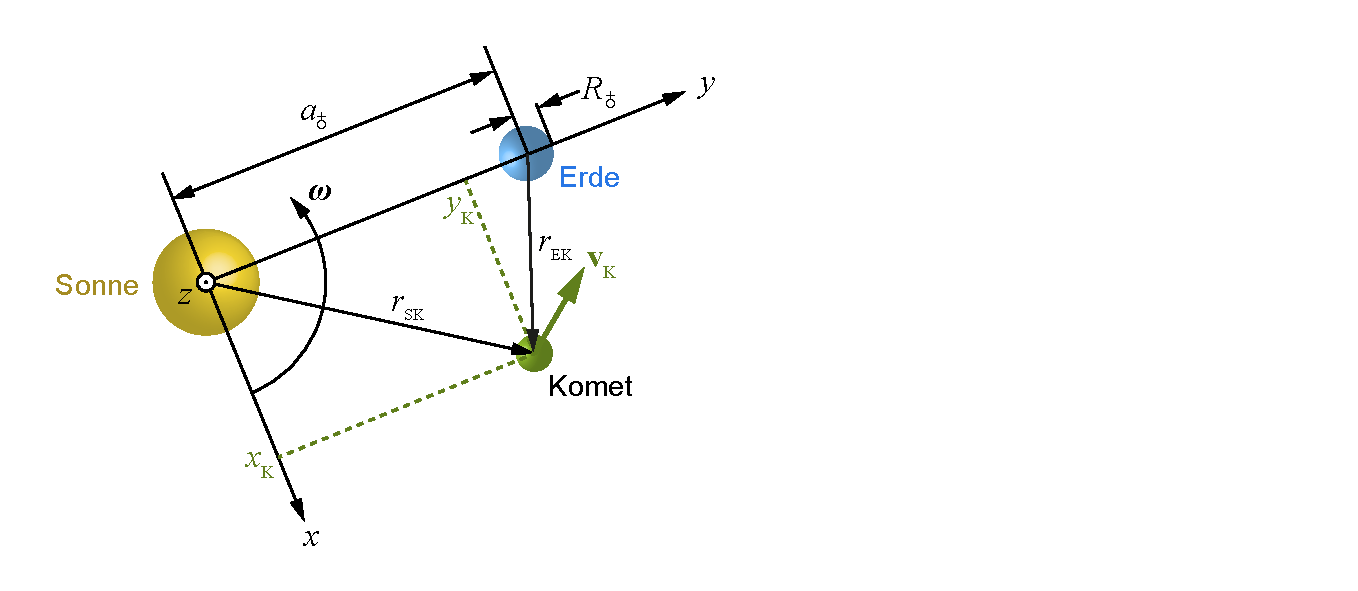
\includegraphics[width=\textwidth]{AufprallKomet.pdf}%
\caption{Zur Berechnung der Aufschlaggeschwindigkeit eines Kometen}%
\label{abb:hm_aufschlaggeschw}%
\end{figure}

F�r den Moment des Aufschlags gilt:
\begin{align}
H_\text{K,A} (r_\text{K}=R_\text{\earth}) &= \frac{v_\text{A}^2}{2} - \frac{\alpha \mu_\text{G}}{R_\text{\earth}} - \frac{\mu_\text{G}}{a_\text{\earth}} - \frac{\omega^2}{2}\,a_\text{\earth}^2 
= \frac{v_\text{A}^2}{2} - \frac{\alpha \mu_\text{G}}{R_\text{\earth}} - \frac{3\mu_\text{G}}{2a_\text{\earth}} ~~. \label{eq:hm_hmlsg_24b_2} 
\end{align}
F�r eine initiale Position mit $r_0\!\gg\! a_\text{\earth}$ k�nnen wir wegen $\alpha\!\gg\! 1$ in \eqref{eq:hm_hmlsg_24b_1} den zweiten Term vernachl�ssigen und erhalten
\begin{equation}
H_{\text{K},0} = \frac{v_0{}^{2}}{2} - \frac{\mu_\text{G}}{r_0} - \frac{\omega^2}{2}\,(x_0{}^{2} + y_0{}^{2}) ~~. 
\end{equation}
Jetzt verlassen wir das rotierende KOS und gehen in das in der Sonne verankerte Inertialsystem �ber. \label{eq:hm_hmlsg_24b_2a} 
Dann gilt f�r die Geschwindigkeit des Himmelsk�rpers in diesem KOS (man beachte die Richtung von $\vec{\omega}$):
\begin{equation}
\vec{v}_0 = \vec{v}_\text{S} - \vec{\omega}\times\vec{r}_\text{S} ~~,\label{eq:hm_hmlsg_24b_3}
\end{equation}
wobei die Indizes S die Gr��en im Inertialsystem der Sonne kennzeichnen. 
Wir k�nnen dann schreiben:
\begin{equation}
v_0{}^2 = v_\text{S}{}^{2} - 2\,\vec{v}_\text{S}(\vec{\omega}\times\vec{r}_\text{S}) + \omega^2({x_\text{S}}^2 + {y_\text{S}}^2) ~~.
\label{eq:hm_hmlsg_24b_4}
\end{equation}
Wir setzen \eqref{eq:hm_hmlsg_24b_4} in \eqref{eq:hm_hmlsg_24b_3} ein und ber�cksichtigen, dass gilt:
\begin{align*}
\vec{r}_0{}^2 &= {x_0}^{2} + {y_0}^{2} = {x_\text{S}}^{2} + {y_\text{S}}^{2} = {\vec{r}_\text{S}}^2 ~~~\text{und} ~~~ \vec{v}_\text{S}(\vec{\omega}\times\vec{r}_\text{S}) = \vec{\omega}(\vec{r}_\text{S}\times\vec{v}_\text{S}) = \vec{\omega}\,\vec{L} \,.
\end{align*}
Hierin ist $\vec{L}$ der konstante Drehimpuls des Kometen im Inertialsystem der Sonne ist.
Somit erhalten wir f�r die Energie
\begin{equation}
H_\text{K,S} = \frac{v_\text{S}^2}{2} - \frac{\mu_\text{G}}{r_\text{S}} - \omega L\cos i_\text{K}~~,
\label{eq:hm_hmlsg_24b_5}
\end{equation}
worin der Winkel $i_\text{K}$ die Neigung der Bahn des Himmelsk�rpers gegen die Ekliptik ist.
Setzen wir wegen der Energieerhaltung $H_\text{K,0}\!=\!H_\text{K,S}\!=\!H_\text{K,A}$, so erhalten wir f�r die Geschwindigkeit $v_\text{A}$ beim Aufschlag:
\begin{equation}
v_\text{A}{}^2 = \frac{2 \alpha \mu_\text{G}}{R_\text{\earth}} + \frac{3\mu_\text{G}}{a_\text{\earth}} + C_\text{J} - 2,\omega L\cos i_\text{K} ~~.
\label{eq:hm_hmlsg_24b_6}
\end{equation}
Darin haben wir die sogenannte Jacobi-Konstante\index{Jacobi-Konstante} $C_\text{J}\!=\!v_0^2 - 2\,\mu_\text{G}/r_0$ eingef�hrt, welche der doppelten spezifischen Energie des Himmelsk�rpers entspricht, wenn dieser nur dem Schwerefeld der Sonne ausgesetzt w�re. Sie dazu auch die Definition $C_\text{J}$ im Kap 1.2.3.6 in Band I.
Wir k�nnen nun mit den Beziehungen \eqref{eq:hm_drehimpuls_von_ae} f�r den Drehimpuls bzw. dem vis-viva-Satz \eqref{eq:hm_vis-viva} die Gr��en $L$ und $H_\text{J}$ durch die geometrischen Bahnparameter $a_\text{K}$ und $e_\text{K}$ ersetzen.
Wir erhalten nach einigen algebraischen Umformungen
\begin{equation}
v_\text{A} = \sqrt{\frac{2\alpha\mu_\text{G}}{R_\text{\earth}} + \underbrace{\frac{\mu_\text{G}}{a_\text{\earth}} \lek 3-\lk \frac{a_\text{\earth}}{a_\text{K}} + 2\cos i_\text{K}\,\sqrt{\frac{a_\text{K}}{a_\text{\earth}}\,(1-e_\text{K}^2)} \rk \rek }_{U^2}} ~~.
\label{eq:hm_hmlsg_24b_7}
\end{equation}
Das ist schon unsere L�sung.
Der erste Term unter der Wurzel ist eine Konstante und nichts anderes als das Quadrat der 2. kosmischen Geschwindigkeit \index{Kosmische Geschwindigkeit}
\begin{equation*}
v_\text{kos,II} = \sqrt{\frac{2\alpha\mu_\text{G}}{R_\text{\earth}}} = \sqrt{\frac{2Gm_\text{\earth}}{R_\text{\earth}}} = 11.2\:\text{km/s}~~.
\end{equation*}
Im zweiten Term unter der Wurzel identifizieren wir einerseits die 3. kosmische Geschwindigkeit
\begin{equation*}
v_\text{kos,III} = \sqrt{\frac{\mu_\text{G}}{a_\text{\earth}}} = 29.7\:\text{km/s}
\end{equation*}
und definieren andererseits den Term in der eckigen Klammer als Funktion $f(a_\text{K},e_\text{K},i_\text{K})$.
Dadurch l�sst sich \eqref{eq:hm_hmlsg_24b_7} deutlich vereinfacht schreiben als
\begin{equation}
v_\text{A} = \sqrt{v_\text{kos,II}^2 + v_\text{kos,III}^2 \, f(a_\text{K},e_\text{K},i_\text{K})} =\sqrt{v_\text{kos,II}^2  + U^2}~~.
\label{eq:hm_hmlsg_24b_8}
\end{equation}
Wir k�nnen die Aufschlaggeschwindigkeit \eqref{eq:hm_hmlsg_24b_8} auch schreiben als
\begin{equation}
v_\text{A} = v_\text{kos,III}\,\sqrt{p_\text{\earth} - \lk \frac{a_\text{\earth}(1-e)}{a_\text{K}} + 2\cos i_\text{K} \sqrt{\frac{(1+e_\text{K})a_\text{K}}{a_\text{\earth}}}\rk}
\label{eq:hm_hmlsg_24b_9}
\end{equation}
mit $p_\text{\earth}\!=\!\lk 3 + 2\alpha a_\text{\earth}/R_\text{\earth} \rk \!\approx\! 3.1411$.
F�r langgestreckte Ellipsen $e\!\rightarrow\! 1$ ist die Periheldistanz $q_\text{K}/(1-e)\!\gg\! a_\text{\earth}$ und $1+e_\text{K}\!\approx\! 2$, so dass \eqref{eq:hm_hmlsg_24b_9} geschrieben werden kann als 
\begin{equation}
v_\text{A} = v_\text{kos,III}\,\sqrt{p_\text{\earth}-2\cos i_\text{K}\sqrt{\frac{2q_\text{K}}{a_\text{\earth}}}} ~~,
\label{eq:hm_hmlsg_24b_10}
\end{equation}
was in der \figref{hm_aufschlaggeschw_2} f�r verschiedene Periheldistanzen und Bahnneigungen dargestellt ist.
Wenn man annimmt, dass der Komet/Meteor bei seiner Periheldistanz die Erde trifft, dann gilt $q_\text{K}=a_\text{\earth}$ und wir k�nnen aus der Abbildung die minimale Aufprallgeschwindigkeit von 16.6 km/s bei $i_\text{K} = 0\degree$ und die maximale von 72.6 km/s bei $i_\text{K} = 180\degree$ ablesen.
\begin{figure}[H]
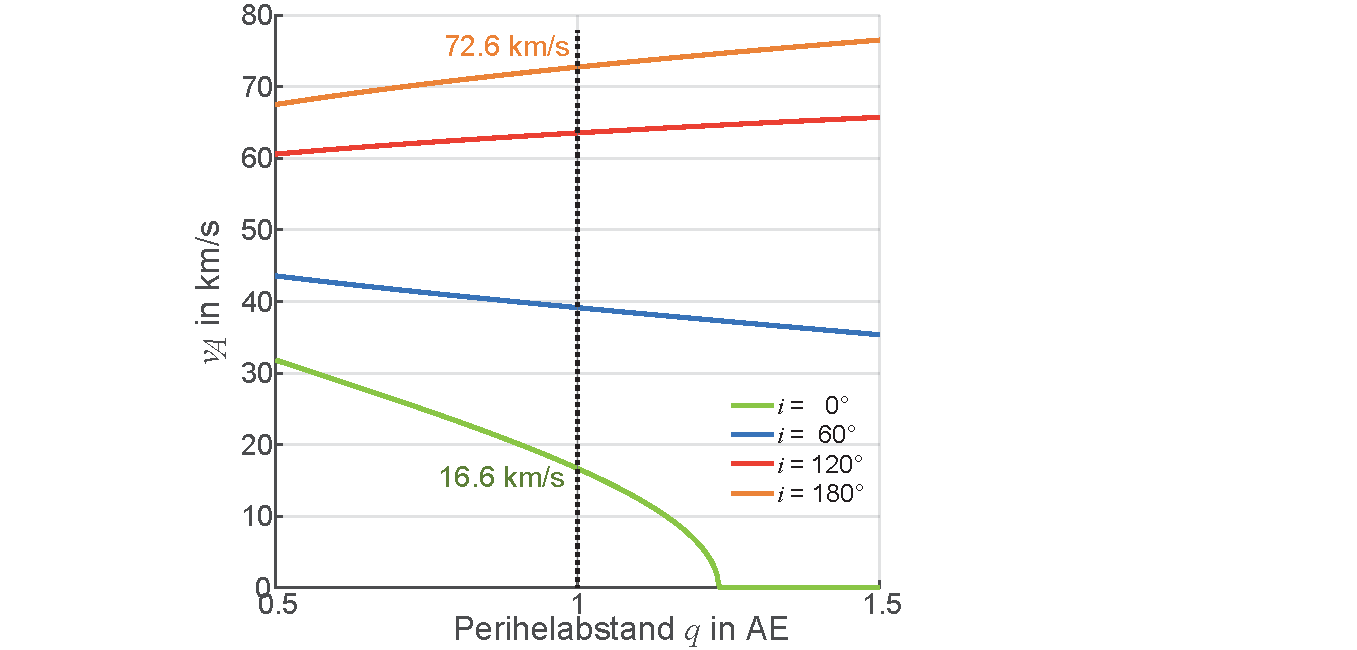
\includegraphics[width=\textwidth]{Aufschlaggeschwindigkeit.pdf}%
\caption[Aufschlaggeschwindigkeit eines Kometen.]{Berechnete Aufschlaggeschwindigkeit eines Kometen f�r verschiedene Bahnneigungen als Funktion des Perihelabstandes.}%
\label{abb:hm_aufschlaggeschw_2}%
\end{figure}

Wir k�nnen \eqref{eq:hm_hmlsg_24b_7} und \eqref{eq:hm_hmlsg_24b_9} auch benutzen, um die im Beispiel \ref{bsp:hm_shoemaker_levy} berechnete Aufschlaggeschwindigkeit des Kometen SL9 zu �berpr�fen.
Wir m�ssen in unseren Gleichungen nur folgende Ersetzungen vornehmen:
\begin{align*}
	a_\text{\earth} &\rightarrow a_\text{\jupiter} = 5.204\:\text{AE} \\
	R_\text{\earth} &\rightarrow R_\text{\jupiter} = 71492\:\text{km} \\
	\alpha &\rightarrow \alpha_\text{\jupiter} = \frac{m_\text{\jupiter}}{m_\text{\astrosun}} = 0.955\cdot 10^{-3} ~~.
\end{align*}
Mit diesen Werten und den Bahnparametern von SL9 aus Tabelle \ref{tab:hm_bahnparameter} erhalten wir $v_\text{A,SL}\!=\!59.5\:\text{km/s}$, was gut mit den numerisch berechneten Werten in Beispiel \ref{bsp:hm_shoemaker_levy} �bereinstimmt.\\

\item Aus \eqref{eq:hm_Shoemaker1979} erh�lt man f�r die kinetische Energien des Meteoriten im N�rdlinger Ries \bzw Steinheimer Becken
\begin{equation*}
T_\text{N} \approx 141\:\text{Gt TNT}  ~~ \text{bzw.} ~~ T_\text{S} \approx 268\:\text{Mt TNT} ~~.
\end{equation*}
Zum Vergleich, die Atombombe von Hiroshima hatte eine Sprengkraft von \anf{nur} ca. $12\:\text{kt TNT}$.
Die Energien von solchen Asteroiden/Meteoriten sind also unglaublich hoch (Man dr�cke diese einmal in konventionellen Gr��en ($1\:$kt TNT entspricht $4.185\cdot 10^{12}\:\text{J}$ aus.).\\
Unter Annahme eines kugelf�rmigen Himmelsk�rpers mit der Dichte $\rho\!=\!2.8\:\text{g/cm}^3$ kann man den Durchmesser des Meteoriten absch�tzen.
Im L�sungsteil (b) (\figref{hm_aufschlaggeschw_2}) hatten wir f�r $v_\text{min}$ und $v_\text{max}$ Werte zwischen 16 und 70 km/s erhalten.
Da es sehr wahrscheinlich ist, dass die Inklination der Asteroidenbahn zwischen $20\degree$ und $45\degree$ lag, k�nnen wir von Aufschlaggeschwindigkeiten zwischen $20$ km/s und $30$ km/s ausgehen.
Es ergeben sich dann Asteroidendurchmesser im Fall des N�rdlinger Ries von
\begin{equation*}
D_\text{N} = 2\,\sqrt[3]{\frac{T_\text{N}}{\pi\rho v_\text{A}^2}} = 1.0\:\text{km}~\ldots~ 1.3\:\text{km}
\end{equation*}
und im Fall des Steinheimer Beckens von
\begin{equation*}
D_\text{S} = = 0.5\:\text{km}~\ldots~ 0.65\:\text{km}~.
\end{equation*}

\begin{figure}[H]
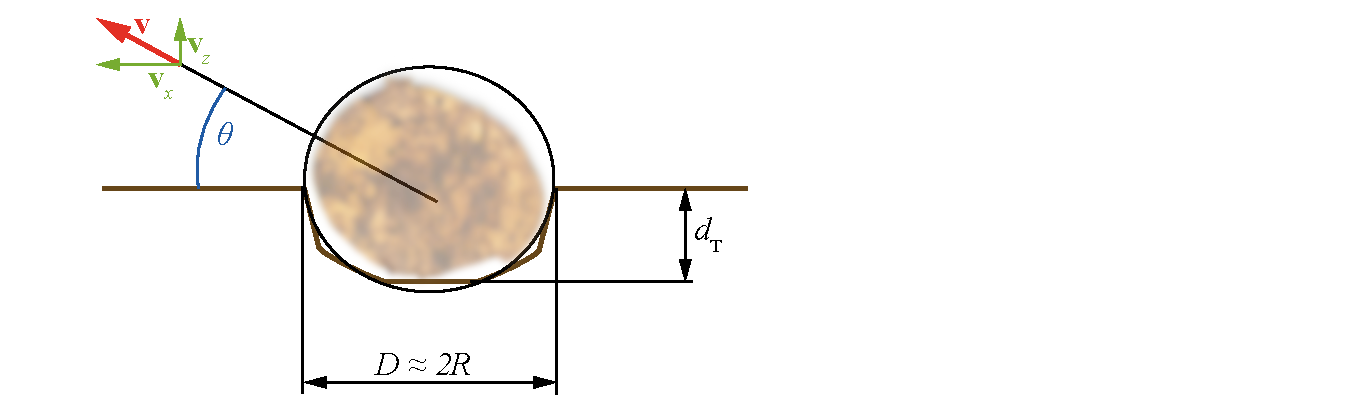
\includegraphics[width=\textwidth]{Meteorkrater.pdf}%
\caption{Zur Berechnung der Aufschlaggeschwindigkeit eines Kometen}%
\label{abb:hm_shoemaker_deriv}%
\end{figure}

Wir wollen jetzt noch eine Absch�tzung f�r die Shoemaker-Formel geben. Dazu nehmen wir an, dass die vom Asteroiden (oder einem anderen Himmelsk�rper) ausgeworfene Kratermasse unter einem Winkel von $\theta$ und mit einer Geschwindigkeit $v$ wegfliegt. Die Mindestzeit, die die ausgeworfene Masse in der Luft sein muss, ergibt sich nach \figref{hm_shoemaker_deriv}
zu:
	\[t = 2 v_z/g = 2v\sin\theta/g
\]
In dieser Zeit muss der Kraterdurchmesser $D=2 R$ "`ausgehoben"' werden, also:
	\[ D = v_x\,t = 2v^2\,\sin\theta \cos\theta/g = v^2 \,\sin(2\theta)/g \leq v^2/g\,
\]
woraus folgt : $v_\text{min} = \sqrt{D\,g}$.
Die Masse des Aushubs ist (Krater als zylinderf�rmig angenommen):
	\[ m_\text{A} = \varrho\frac{\pi}{4}\,D^2\,d_\text{T}\,,
	\]
	mit $\varrho \approx \SI{4e3}{\kg\per\metre\cubed}$.
Damit ist eine minimale kinetische Energie verbunden, die den Auswurf "`wegtransportiert"';
	\[ T_\text{min} = \frac{m_\text{A}}{2} \,v^2 = \frac{\pi}{8}\varrho\,g\,d_\text{T}\,D^3\,.
	\]
Ber�cksichtigt man noch, dass wegen der Umwandlung in thermische Energie nur wenige Prozent $\eta = 1\% \ldots 4\%$ in kinetische Energie umgewandelt werden, dann gilt die Beziehung:
\begin{align}
T_\text{min}  = \tilde{\kappa}\,	T_\text{K} = \tilde{\kappa} \frac{\pi}{8}\varrho\,g\,d_\text{T}\,d_\text{T}\,D^3\,. \,. \label{eq:hm_shoemaker_verified}
\end{align}
Wir bekommen also ann�hernd den empirischen Zusammenhang $D \propto T_\text{K}^{1/3}$, wobei wegen $\tilde{\kappa} = \tilde{\kappa}(d)=\tilde{\kappa}(d(D))$ eine zus�tzliche $D-$Abh�ngigkeit ergibt, die sich in der Shoemaker-Formel im Exponenten zeigt. Wir �berlassen es dem Leser, in Formel \eqref{eq:hm_shoemaker_verified} den Proportionalit�tsfaktor $\tilde{\kappa}$ auszurechnen und zu verifizieren, dass sich tats�chlich solche gigantischen Energien ergeben.\\

\item Nehmen wir an, dass der Planetoid (Meteor) mit Masse $m_\text{P}$ einen Mond der Masse $m_\text{M}$ hatte.
  Dann zieht der Planetoid den Mond mit der Kraft $F_\text{P}\!=\! Gm_\text{P}m_\text{M}/d^2$ an.
  Andererseits wirkt auf die beiden K�rper die Gravitationskraft der Sonne in unterschiedlichem Ma�e (Gezeitenkraft) (siehe \kap{hm_gezeiten}), die die beiden K�rper zu trennen versucht. F�r f�r die Gezeitenkraft gilt:
\begin{equation*}
F_\text{Gez} \approx \frac{2Gm_\text{M}m_\text{\astrosun}\,a_\text{PM}}{a_\text{\earth}^3}~~,
\end{equation*}  
worin $a_\text{PM}$ der Abstand zwischen Planetoid und Mond ist.
Das System des Doppelplanetoiden (bzw. Planetoid mit Mond) ist stabil, wenn $F_\text{P}\!>\!F_\text{Gez}$, also
\begin{equation*}
\frac{Gm_\text{P}m_\text{M}}{a_\text{PM}{}^2} > \frac{2Gm_\text{M}m_\text{\astrosun}\, a_\text{PM}}{a_\text{\earth}^3}~~.
\end{equation*}
Dies ist erf�llt, wenn
\begin{equation*}
	a_\text{PM} < \sqrt[3]{\frac{m_\text{P}}{2m_\text{\astrosun}} a_\text{\earth}^3} = a_\text{\earth}\,\sqrt[3]{\frac{m_\text{P}}{2m_\text{\astrosun}}} ~~.
\end{equation*}
Mit der Masse $m_\text{P}\!=\!\rho_\text{P}V_\text{P}$ aus Aufgabenteil (c) erhalten wir $a_\text{PM}\!\leq\! 150\:$km.
Verglichen mit dem Abstand der beiden Einschlagkrater von $40\:$km ist es also wahrscheinlich oder zumindest m�glich, dass der Doppelkrater vor 15 Millionen Jahren durch einen Doppelplanetoiden bzw. Planetoid und zugeh�riger Mond verursachte wurde.
\end{enumerate}
Die �bungsaufgabe und deren L�sung basiert auf der Darstellung �hnlicher Probleme in \cite{Garfinkle2014} und \cite{Quetz2017}.
Wir verweisen auch auf das entsprechende \mscr~\mlhmref{VerweildauerKomet.m} sowie \mlhmref{AufprallgeschwindigkeitKomet.m}.
\medskip \end{sol}

\textcolor{blue} {$\rightarrow$ zur} \probref{hm_verweildauer_komet_erdbahn}.\\
\noindent\rule[1ex]{\textwidth}{0.5pt} \newpage


%-----------------------------------------------------------------------------------------------------------

\begin{sol}{prob:hm_Doppelstern}\label{lsg:hm_Doppelstern} %�bung27
\textbf{Doppelstern-System - Vergleich numerische und analytische L�sung} \\ \\

Die Rechnungen finden sich f�r ein Modellsystem mit Massenverh�ltnis 2.5:1 und einem anf�nglichen Abstand von 2\,AE, sowie anf�nglichen Geschwindigkeiten in Oppositionsstellung von $v_0 = \SI{-5}{\km\per\second}$ \bzw $v_0 = \SI{20}{\km\per\second}$ in den \mscr en \mlhmref{Doppelsternsystem.m} (Inertialsystem) \bzw \mlhmref{DoppelsternsystemCOM.m} (Schwerpunktsystem). L�sungen sind beispielhaft in den folgenden Abbildungen gezeigt.\\
%Die numerische �bereinstimmung mit der analytischen L�sung ist ausgezeichnet.
\begin{figure}[H]
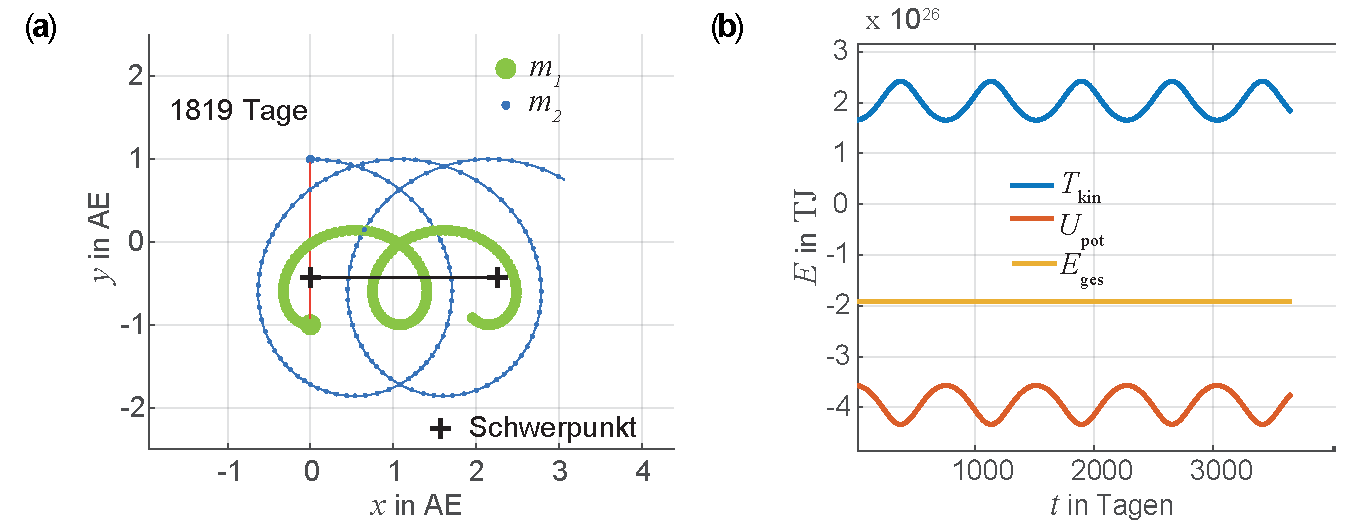
\includegraphics[width=\textwidth]{DoppelsternEnergie.pdf}%
\caption{Trajektorie \fa und Energieanteile \fb eines Doppelsternsystems im Inertialsystem. Die Energieerhaltung mit dem Hin-und Herpendeln zwischen kinetischer und potentieller Energie ist gut zu erkennen}%
\label{abb:hm_doppelsternenergie}%
\end{figure}
\begin{figure}[H]
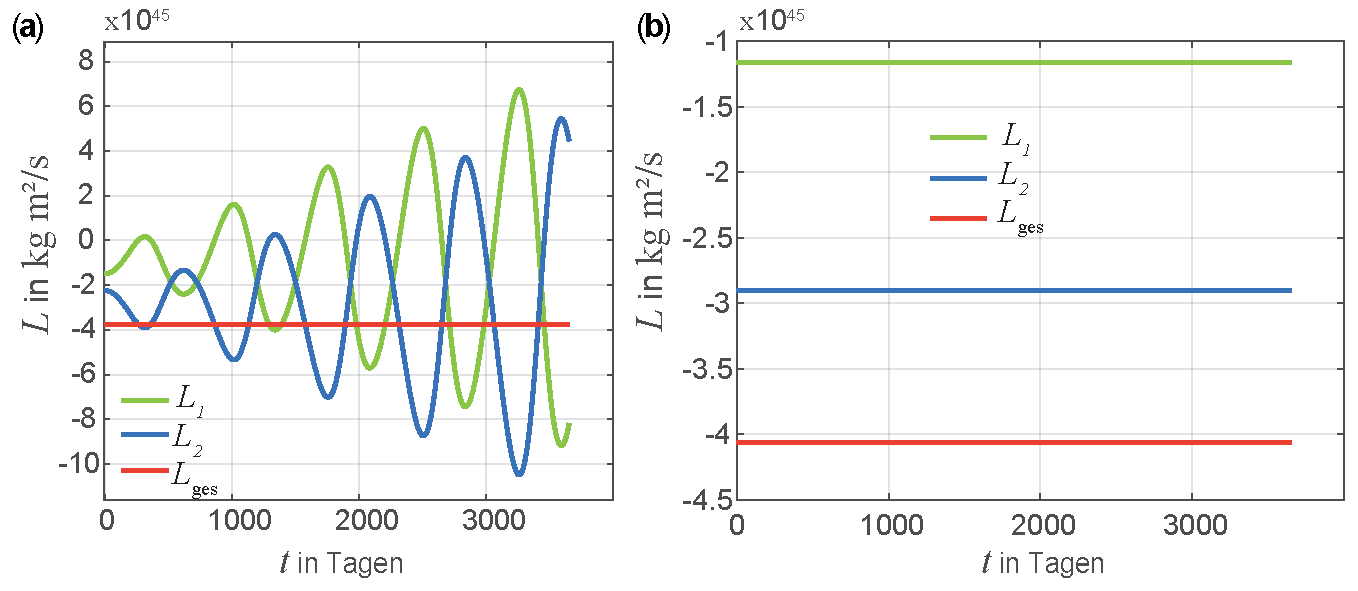
\includegraphics[width= \textwidth]{DoppelsternDrehimpulse.pdf}%
\caption{Drehimpulse eines Doppelsternsystems im Inertialsystem \fa und im Schwerpunktsystem \fb. Im Inertialsystem ist der Gesamtdrehimpuls erhalten}%
\label{abb:hm_doppelsterndrehimpulse}%
\end{figure}
\end{sol}
\textcolor{blue} {$\rightarrow$ zur} \probref{hm_Doppelstern}.\\
\noindent\rule[1ex]{\textwidth}{0.5pt} \newpage

%-----------------------------------------------------------------------------------------------------------

\begin{sol}{prob:hm_Sonnensystem}\label{lsg:hm_Sonnensystem} %�bung28
\textbf{Sonnensystem - Numerische, Kepler- und JPL-Berechnung} \\ \\

Wir verweisen auf die \mscr e \mlhmref{SonnensystemSimulationKepler.m}, \mlhmref{SonnensystemSimulationJPL.m} und \mlhmref{SonnensystemSimulationLangeZeiten.m}.\\
Als Referenzdaten verwenden wir die Vektordaten aus \url{https://ssd.jpl.nasa.gov/horizons/} (\cite{JPL2020}).

Die Bewegungsgleichungen f�r die Beschleunigungen der einzelnen ($i,j = 1 \ldots 8$) Planeten und die beiden betrachteten Kometen ($i,j = 9,10$) und die Sonne ($i,j = =N=11$) lauten dann:
	\begin{align}
		 \vec{a}_i = \ddot{\vec{r}}_i = -\sum_{j, j \neq i}^{N} (\vec{r}_i-\vec{r}_j) \frac{G\,m_i}{|\vec{r}_i-\vec{r}_j|^3}~~~~i=1 \ldots N~\,. \label{eq:hm_PlanetenDGLSystem01}
	\end{align}
Hierin sind $\vec{r}_i$ und $m_i$ die Positionsvektoren \bzw die Massen der einzelnen Planeten,  Kometen und der Sonne. Der Index $i,kj=N+1$ bezieht sich dabei auf die Sonne.
Die DGLs \eqref{eq:hm_PlanetenDGLSystem01} werden mit den entsprechenden Anfangsbedingungen f�r die Himmelsk�rper numerisch integriert. 

In \figref{hm_SonnensystemSimulation01} vergleichen wir die Abweichungen der L�sungen f�r \eqref{eq:hm_PlanetenDGLSystem01}, die wir aus der L�sung der Kepler-Gleichung \bzw der St�rungstheorie und zum anderen �ber numerische Integration von \eqref{eq:hm_PlanetenDGLSystem01} erhalten haben. Die Anfangswerte $\vec{r}_i(t_0)$ und $\dot{\vec{r}}_i(t_0)$  beschaffen wir uns aus dem JPL-Webservice \url{https://ssd.jpl.nasa.gov/horizons/}. Bei der Erdbahn erkennt eine periodische Abweichung (im Monatsrhythmus) unserer Rechnung von der JPL-Berechnung, die nat�rlich, davon herr�hrt, dass wir den Mond in unseren Rechnungen nicht ber�cksichtigt haben. Ansonsten ist die �bereinstimmung aber sehr gut und die Rechnung viel genauer als die einfache Kepler-L�sung, was man auch an der berechneten Marsbahn sehr gut sieht (bei der ja kein Mond der Gr��enordnung des Erdmondes zu ber�cksichtigen ist). Wir empfehlen dem interessierten Leser, die Rechnungen unter Ber�cksichtigung des Mondes zu wiederholen.

\begin{figure}[H]
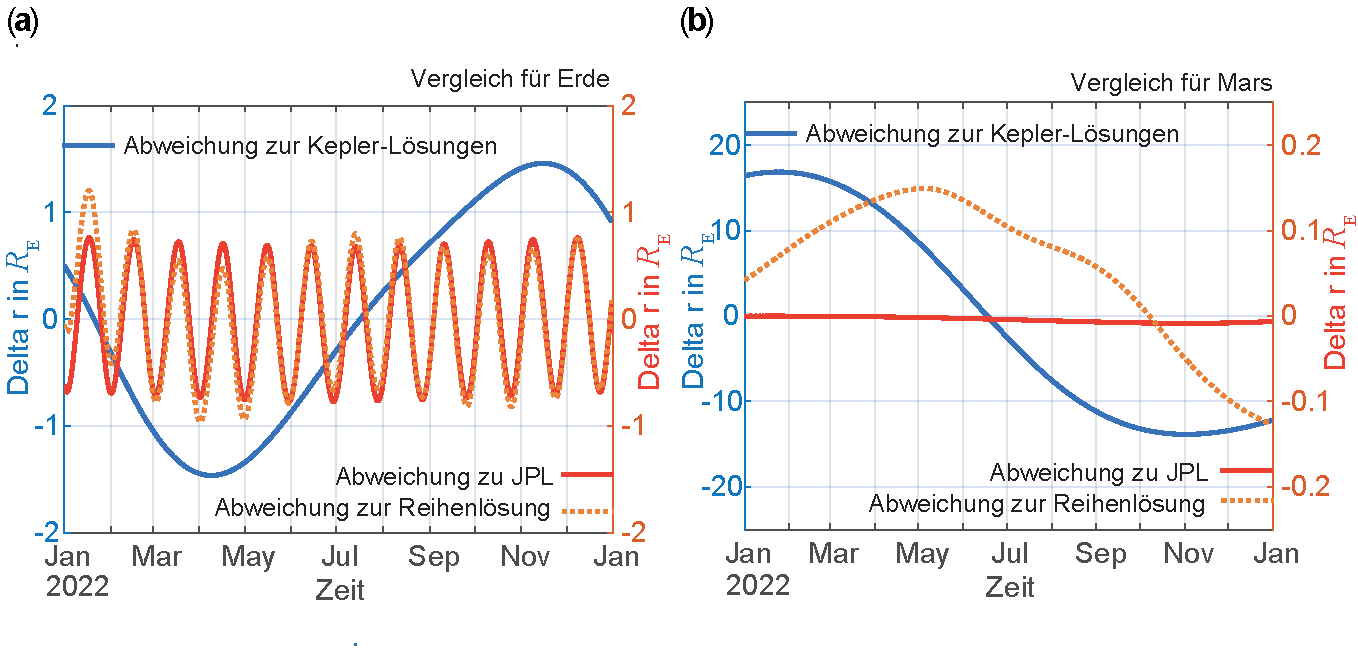
\includegraphics[width=\textwidth]{SonnensystemSimulation01.pdf}%
\caption[Sonnensystem-Simulation durch numerischen L�sung der Newtonschen Bewegungsgleichungen.]{Sonnensystem-Simulation durch numerischen L�sung der Newtonschen Bewegungsgleichungen. Abweichungen der L�sungen f�r die Bahn der Erde \fa und des Mars \fb von den Referenzdaten des JPL (\url{https://ssd.jpl.nasa.gov/horizons/}). Zum Vergleich sind auch die Abweichungen zur einfachen Kepler-L�sung und zur Reihenentwicklung nach der St�rungstheorie (\kap{Reihenentwicklung}) gezeigt.}%
\label{abb:hm_SonnensystemSimulation01}%
\end{figure}

In \figref{hm_SonnensystemSimulation02} zeigen wir die berechnete Bewegung des Schwerpunktes gegen�ber der Ausgangsposition. Eigentlich sollte dieser ja nach Definition in der Nulllage verbleiben. Die sehr kleine (man beachte die Achseneinteilung) systematische Drift resultiert aus der Tatsache, dass wir ja nicht �ber alle K�rper des Sonnensystems integriert haben. Es feheln ja etliche Monde, Kometen und Asteroiden. Die Gr��e der Drift ist f�r uns auch eine Aussage zur Genauigkeit der Integration.\\
%Es ist gar nicht so einfach die Frage zu beantworten, wie man f�r das Sonnensystem den Ursprung des Inertialsystems findet. Die IAU (\textit{International Astronomical Union}) hat �ber sehr pr�zise (\textit{Very Large Base Interferometry} - VLBI) Messungen
%von extra-galaktischen Quellen das sogenannte ICRF3-Koordinatensystem (International Celestial Reference Frame 3) definiert. Der Schwerpunkt dessen Sonnensystems (\textit{Solar System Bary Center}-SSBC) wird (nicht-relativistisch) definiert durch:
% 	\begin{align}
%		 \vec{R}_\text{SSBC}  = \lk \sum_j  m_i\vec{r}_i\rk \bigg/ \lk \sum_j m_j \rk \,, \label{eq:hm_PlanetenDGLSystem02}
%	\end{align}
%wobei �ber alle K�rper des Sonnensystems summiert wird.\\
%Der Leser wird m�glicherweise auch die Frage stellen, wie die hochgenauen Daten des JPL zustande kommen. Keine Frage, die Ephemeriden des JPL sind sehr gut, aber sie sind sicherlich nicht auf den Bruchteil eines Millimeters genau, obwohl sie mit so vielen Dezimalstellen angegeben werden. Zur Erstellung einer JPL Ephemeride weren mehrere Beobachtungsdaten (optische, Radardaten und Raumfahrzeug-Daten) mit dynamischen Modellen kombiniert, insofern ist die JPL Ephemeride eine "`gemischt beobachtete-gerechnete"' Ephemeride und hat sowohl als Messwert als auch Modellergebnis Ungenauigkeiten. Es wird eine optimale Anpassung entwickelt, um diese Fehler statistisch zu minimieren. Die resultierende Ephemeride ist mit einer stark reduzierten Unsicherheit verbunden. Obwohl die Vektordaten des JPL mit 16 Dezimalstellen ausgegeben werden, bedeutet das nicht, dass alle Ziffern physikalisch sinnvoll sind. Die gesamte Zahl der Stellen wird bei unseren Rechen- und Modellgenauigkeiten nat�rlich nicht ben�tigt. 

\begin{figure}[H]
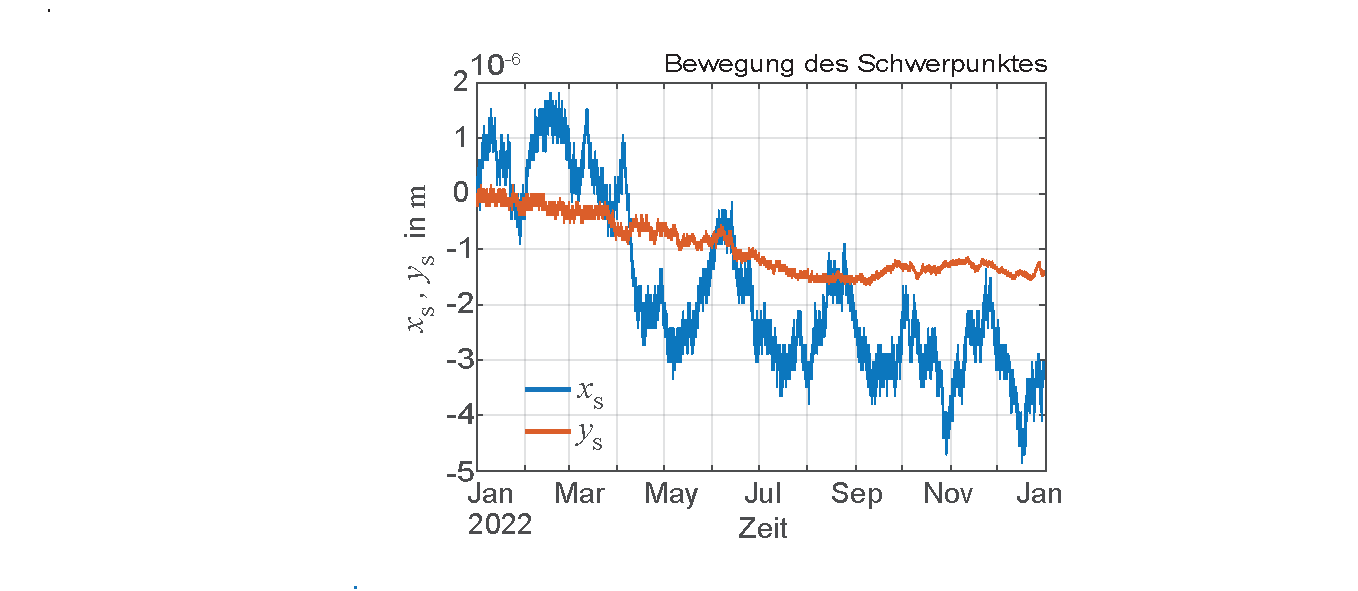
\includegraphics[width=\textwidth]{SonnensystemSimulation02.pdf}%
\caption[Sonnensystem-Simulation durch numerischen L�sung der Newtonschen Bewegungsgleichungen. Bewegung des Schwerpunktes.]{Sonnensystem-Simulation durch numerischen L�sung der Newtonschen Bewegungsgleichungen. Bewegung des Schwerpunktes.}%
\label{abb:hm_SonnensystemSimulation02}%
\end{figure}

In \figref{hm_SonnensystemSimulation03} vergleichen wir die numerischen L�sungen f�r \eqref{eq:hm_PlanetenDGLSystem01} f�r einen Zeitraum von 110 Jahren und \figref{hm_SonnensystemSimulation04} zeigt die Bewegung der Sonne aus der numerischen Integration von  \eqref{eq:hm_PlanetenDGLSystem01} relativ zum Baryzentrum des Sonnensystems (\mscr{}~ \mlhmref{SonnensystemSimulationLangeZeiten.m}) f�r den gleichen Zeitraum.

\begin{figure}[H]
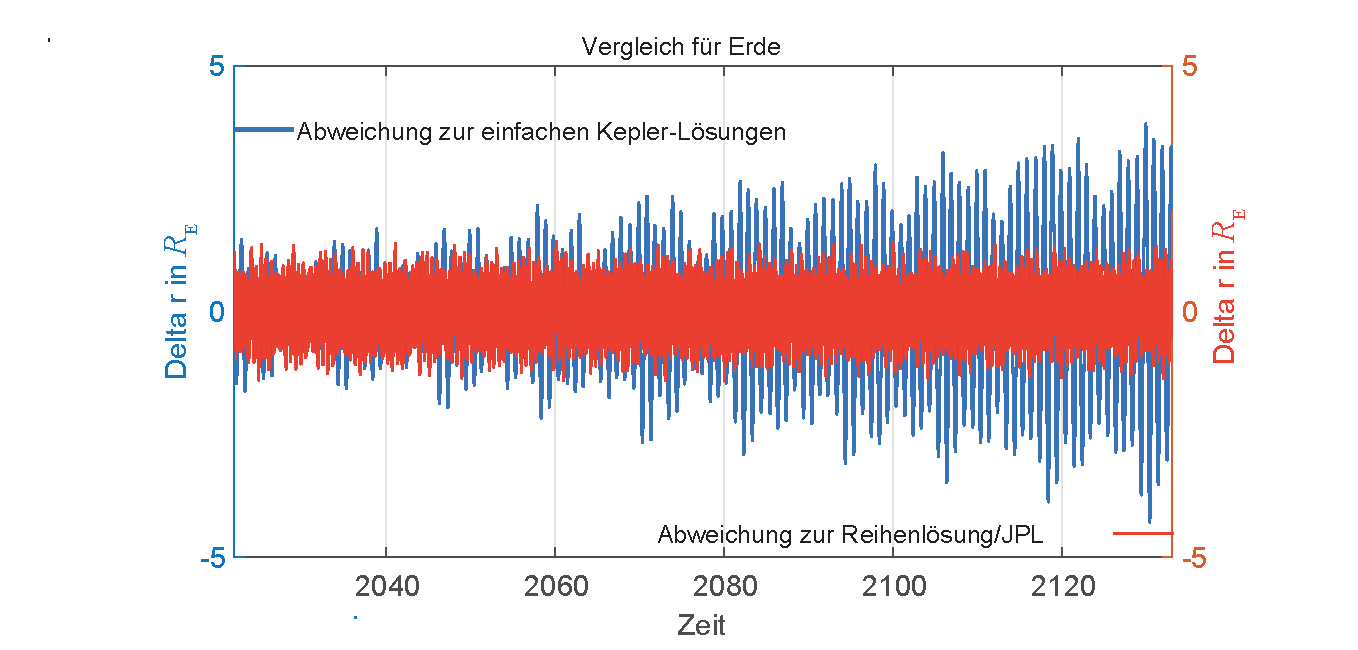
\includegraphics[width=\textwidth]{SonnensystemSimulation03.pdf}%
\caption[Sonnensystem-Simulation durch numerischen L�sung der Newtonschen Bewegungsgleichungen �ber lange Zeiten.]{Sonnensystem-Simulation durch numerischen L�sung der Newtonschen Bewegungsgleichungen �ber lange Zeiten. Abweichungen der L�sungen f�r die Bahn der Erde von den Referenzdaten des JPL (\url{https://ssd.jpl.nasa.gov/horizons/}). Zum Vergleich sind auch die Abweichungen der einfachen Kepler-L�sung zu den JPL Daten gezeigt.}%
\label{abb:hm_SonnensystemSimulation03}%
\end{figure}

\begin{figure}[H]
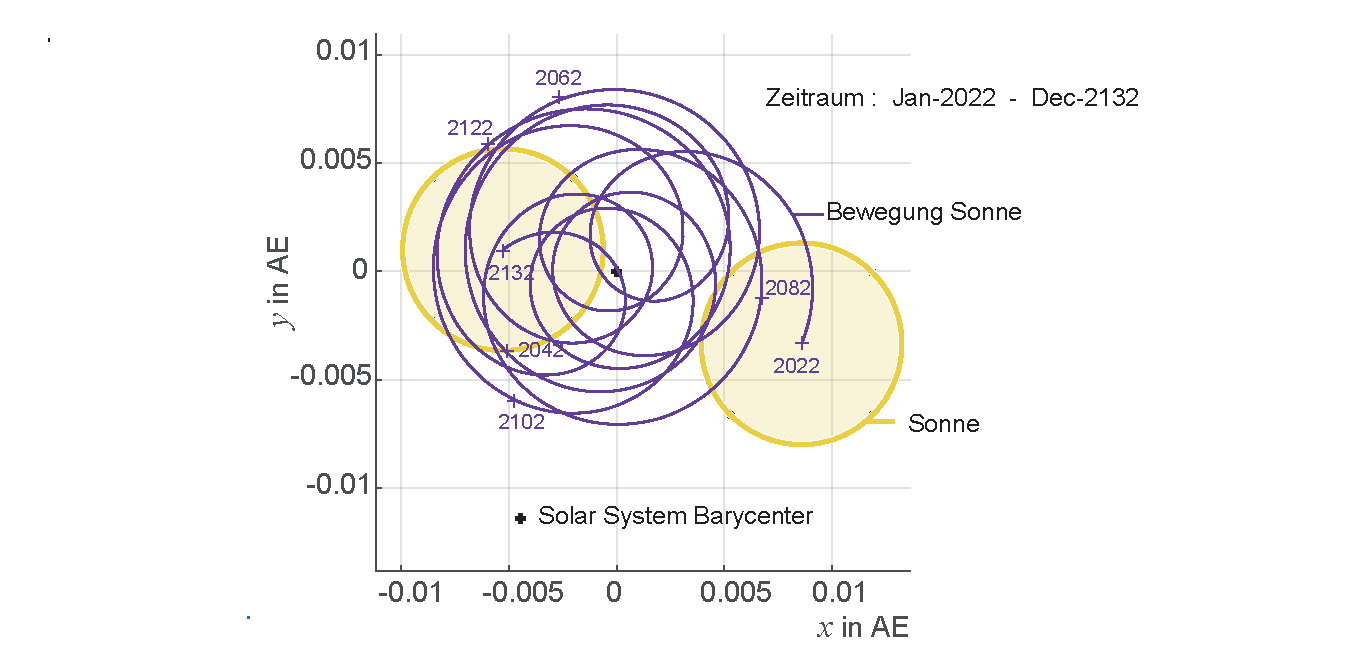
\includegraphics[width=\textwidth]{SonnensystemSimulation04.pdf}%
\caption[Sonnensystem-Simulation durch numerischen L�sung der Newtonschen Bewegungsgleichungen. Bewegung der Sonne im ICRF �ber 120 Jahre.]{Sonnensystem-Simulation durch numerischen L�sung der Newtonschen Bewegungsgleichungen. Bewegung der Sonne im ICRF �ber 110 Jahre. Die Anfangswerte $\vec{r}_i(t_0)$ und $\dot{\vec{r}}_i(t_0)$ haben wir uns wieder aus dem JPL-Webservice beschafft. Vergleiche dazu auch die Ergebnisse in \cite{Park2021}}%
\label{abb:hm_SonnensystemSimulation04}%
\end{figure}

Es ist gar nicht so einfach die Frage zu beantworten, wie man f�r das Sonnensystem den Ursprung des Inertialsystems findet. Die IAU ((\textit{International Astronomical Union})) hat �ber sehr pr�zise (\textit{Very Large Base Interferometry} - VLBI) Messungen
von extra-galaktischen Quellen das sogenannte ICRF3-Koordinatensystem (International Celestial Reference Frame 3) definiert. Der Schwerpunkt dessen Sonnensystems (\textit{Solar System Bary Center}-SSBC) wird (nicht-relativistisch) definiert durch:
 	\begin{align}
		 \vec{R}_\text{SSBC}  = \lk \sum_j  m_i\vec{r}_i\rk \bigg/ \lk \sum_j m_j \rk \,, \label{eq:hm_PlanetenDGLSystem03}
	\end{align}
wobei �ber alle K�rper des Sonnensystems summiert wird.\\
Der Leser wird m�glicherweise auch die Frage stellen, wie die hochgenauen Daten des JPL zustande kommen. Keine Frage, die Ephemeriden des JPL sind sehr gut, aber sie sind sicherlich nicht auf den Bruchteil eines Millimeters genau, obwohl sie mit so vielen Dezimalstellen angegeben werden. Zur Erstellung einer JPL Ephemeride weren mehrere Beobachtungsdaten (optische, Radardaten und Raumfahrzeug-Daten) mit dynamischen Modellen kombiniert, insofern ist die JPL Ephemeride eine "`gemischt beobachtete-gerechnete"' Ephemeride und hat sowohl als Messwert als auch Modellergebnis Ungenauigkeiten. Es wird eine optimale Anpassung entwickelt, um diese Fehler statistisch zu minimieren. Die resultierende Ephemeride ist mit einer stark reduzierten Unsicherheit verbunden. Obwohl die Vektordaten des JPL mit 16 Dezimalstellen ausgegeben werden, bedeutet das nicht, dass alle Ziffern physikalisch sinnvoll sind. Die gesamte Zahl der Stellen wird bei unseren Rechen- und Modellgenauigkeiten nat�rlich nicht ben�tigt. 
Sehr lesenswert zu diesem Thema ist f�r interessierte Leser die Referenz \cite{Park2021}.

\medskip \end{sol}

\textcolor{blue} {$\rightarrow$ zur} \probref{hm_Sonnensystem}.\\
\noindent\rule[1ex]{\textwidth}{0.5pt} \newpage

%-----------------------------------------------------------------------------------------------------------

\begin{sol}{prob:hm_Dreifachstern}\label{lsg:hm_Dreifachstern} %�bung29
\textbf{Dreik�rper-System - L�sung f�r 3 identische Massen} 
\begin{itemize}
	\item \textit{\textbf{Anordnung 1 - Achtf�rmige Trajektorien}}\\

Die Rechnungen sind im \mscr{}~ \mlhmref{DreiKoerperProblem01.m} hinterlegt.
\begin{figure}[H]
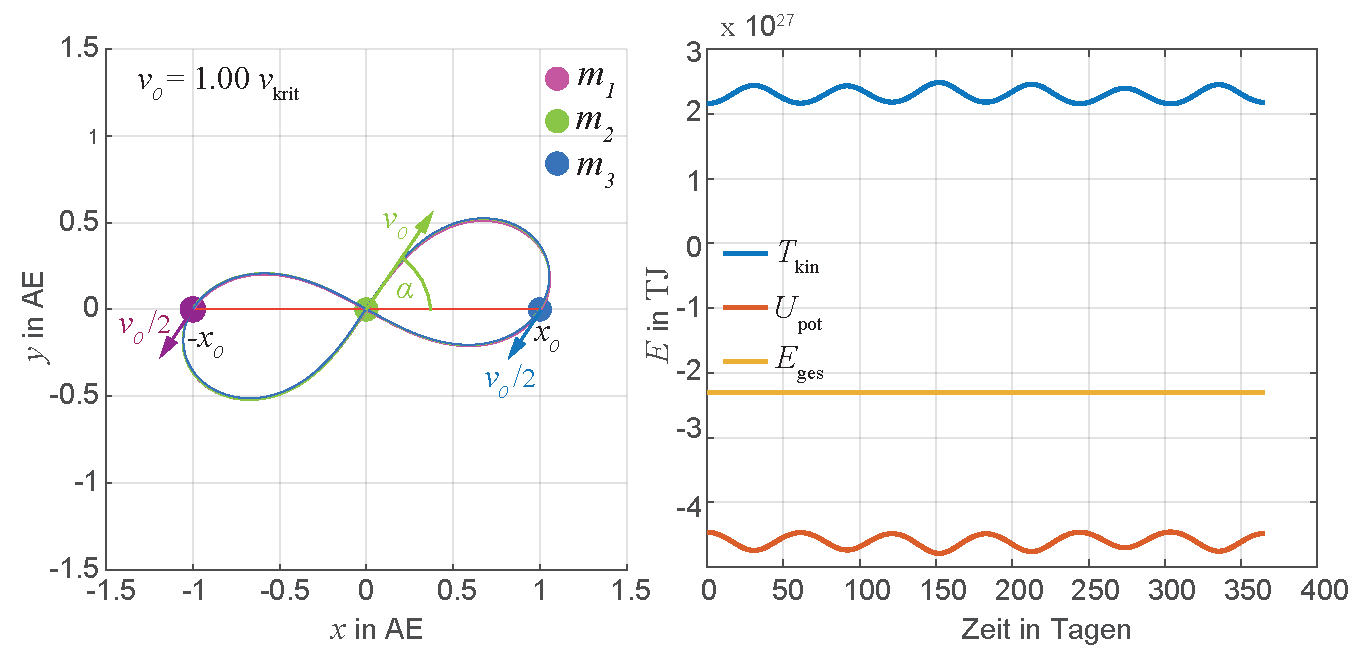
\includegraphics[width=0.9\textwidth]{DreiKoerperSystem01.pdf}%
\caption[Dreik�rperproblem mit Bewegung in Form einer Acht.]{Dreik�rperproblem mit Bewegung in Form einer Acht. Die Geschwindigkeit $v_0=v(t_0)$ ist genau der kritischen Geschwindigkeit $v_\text{krit} = 1.27\,\sqrt{G \, m / x_0}$, worin $2\,x(t_0)$ der Anfangsabstand der beiden �u�eren Massen $m_1$ und $m_3$ auf der $x$-Achse ist. Der Winkel von $\vec{v}_0$ zur $x$-Achse betr�gt $56.9\degree$ \cite{Moore1993, Chenciner2000}. Man erh�lt in diesem Fall stabile Bahnen.}
\label{abb:hm_DreiKoerperSystem01}%
\end{figure}
\begin{figure}[H]
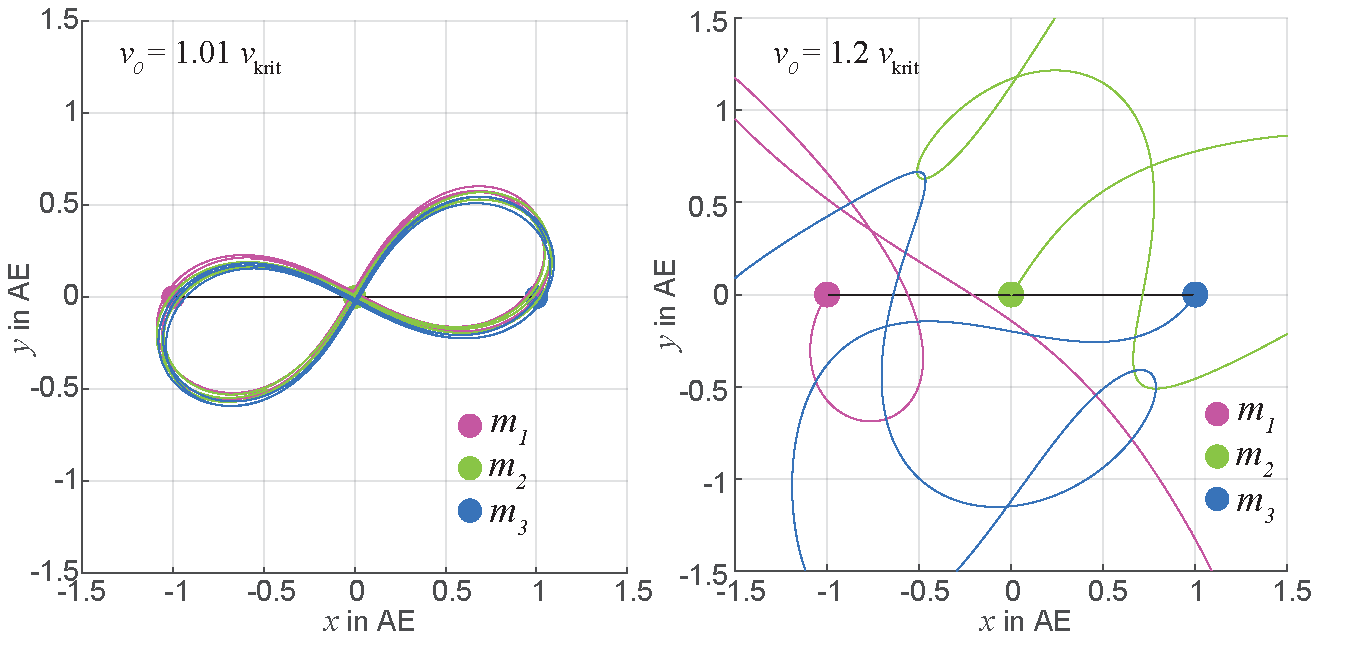
\includegraphics[width=0.9\textwidth]{DreiKoerperSystem02.pdf}%
\caption[Dreik�rperproblem mit Bewegung in Form einer Acht.]{Dreik�rperproblem mit Bewegung in Form einer Acht. Die Geschwindigkeit $v_0$ weicht 1\% (linkes Bild) \bzw 20\% von der der kritischen Geschwindigkeit $v_\text{krit} = 1.27\,\sqrt{(G \, m_0 / x_0)}$ ab. Man erkennt, dass man im linken Bild noch quasistabile Bahnen bekommt, im Fall rechts geht das System sehr schnell in einen chaotischen Zustand �ber.}
\label{abb:hm_DreiKoerperSystem02}%
\end{figure}
	
\newpage
	\item \textit{\textbf{Anordnung 2 - Gleichseitiges Dreieck}}\\
	
Wir k�nnen f�r diesen Fall auf Grund der Symmetrie leicht ableiten, dass die resultierende Kraft aus der Gravitation von den zwei anderen Massen auf die betrachtete betrachtete Masse (in \figref{hm_DreiKoerperSystemDreieck} $m_1$) jeweils in Richtung gemeinsamer Schwerpunkt zeigt und damit als Radialkraft die Massen auf eine kreisf�rmige Umlaufbahn zwingt. (Der Radius der Bahn ist dann gerade der Radius des Umkreises des gleichseitigen Dreiecks.)

\begin{figure}[H]
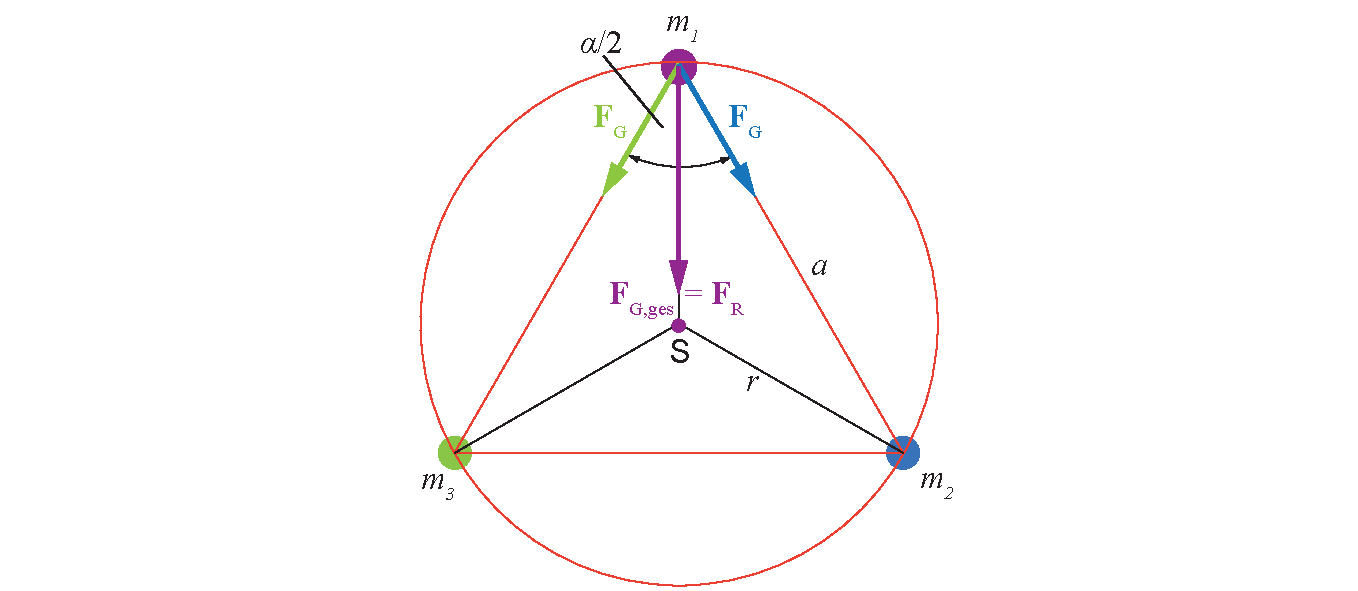
\includegraphics[width=0.9\textwidth]{DreiKoerperSystemDreieck.pdf}%
\caption[Geometrie des Dreik�rperproblem in Form eines gleichseitigen Dreiecks mit Drehung um Schwerpunkt. ]{Geometrie des Dreik�rperproblems in Form eines gleichseitigen Dreiecks mit Drehung um Schwerpunkt.}
\label{abb:hm_DreiKoerperSystemDreieck}%
\end{figure}

Wir wollen die Umlaufgeschwindigkeit berechnen. Dazu berechnen wir mit der Geometrie von \figref{hm_DreiKoerperSystemDreieck} die Gesamtkraft der Massen $m_2=m$ und $m_3=m$ auf die Masse $m_1=m$ zu:
\begin{align}
	\vec{F}_\text{G,ges} &=\frac{G m_1 m_2}{a^2}\,\begin{pmatrix} -\sin(\alpha/2) \\ \cos(\alpha/2 )\\ \end{pmatrix} + 
	        \frac{G m_1 m_3}{a^2}\,\begin{pmatrix} \sin(\alpha/2) \\ \cos(\alpha/2 )\\ \end{pmatrix} \nonumber \\
					&= 2\,\frac{G m^2}{a^2}\,\cos(\alpha/2)\, \veceY~~~~~\text{und mit}~\cos(\alpha/2)=\sqrt{3}/2~\text{, sowie}~d=r\,\sqrt{3} \,\nonumber \\
					&=\frac{G m^2}{\sqrt{3}\,r^2}\,\veceY\,.
	\label{eq:hm_DreiKoerperSystem01}				
\end{align}
Diese muss gleich der Radialkraft der Kreisbewegung sein, \dh:
\begin{align}
	\vec{F}_\text{R} &= \frac{m\,v^2}{r}\,\veceY = \frac{G m^2}{\sqrt{3}\,r^2}\,\veceY\,. 
	\label{eq:hm_DreiKoerperSystem02}				
\end{align}
Damit ergibt sich die Beziehung f�r die Geschwindigkeit: 
\begin{align}
	v = \sqrt{\frac{G\,m}{r\sqrt{3}}} = \sqrt{\frac{G\,m}{a}}\,.
	\label{eq:hm_DreiKoerperSystem03}				
\end{align}

F�r die Simulation im \mscr{}~ \mlhmref{DreiKoerperProblem02.m}\, nehmen wir einen Radius von einer Astronomischen Einheit und eine Masse der K�rper von zwei Sonnenmassen an. Wir erwarten daher eine Bewegung, die sich in der Zeitskala von Jahren abspielt. Das Programm simuliert 10-15 Jahre in Zeitschritten von einem Tag.
	
\begin{figure}[H]
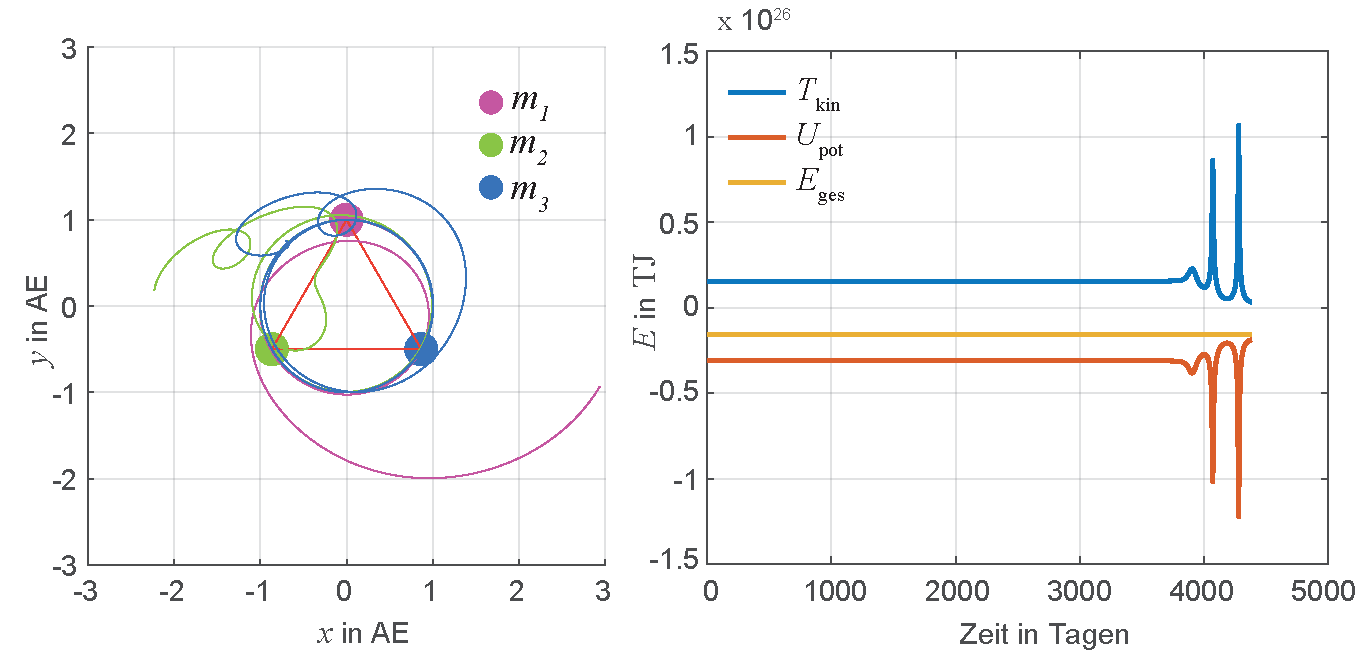
\includegraphics[width=0.9\textwidth]{DreiKoerperSystem03.pdf}%
\caption[Dreik�rperproblem in Form eines gleichseitigen Dreick mit Drehung um Schwerpunkt. ]{Dreik�rperproblem in Form eines gleichseitigen Dreiecks mit Drehung um Schwerpunkt. Man erkennt, dass das System nach einer anf�nglich stabilen Bahn in in einen chaotischen Zustand �bergeht. Dieser �bergangszeitpunkt (in unserem Fall in etwa bei \ca 10 Jahren) h�ngt stark von den Ungenauigkeiten der numerischen Rechnung ab. Man variiere dazu die Toleranzparameter in der options-Funktion des \odevf-Solvers.}
\label{abb:hm_DreiKoerperSystem03}%
\end{figure}
\end{itemize}

\medskip \end{sol}

\textcolor{blue} {$\rightarrow$ zur} \probref{hm_Dreifachstern}.\\
\noindent\rule[1ex]{\textwidth}{0.5pt} \newpage

%-----------------------------------------------------------------------------------------------------------

\begin{sol}{prob:hm_Tempel1_SwiftTuttle}\label{lsg:hm_Tempel1_SwiftTuttle} %�bung30
\textbf{Kometen im Sonnensystem -- Kollision mit der Erde?} \\ \\


Wir verweisen auf die \mscr e \mlhmref{KometenKollisionKepler.m}, \mlhmref{KometenKollisionSim.m} und \mlhmref{KometenKollisionJPL.m}.\\
Als Referenzdaten verwenden wir die Vektordaten aus \url{https://ssd.jpl.nasa.gov/horizons/} (\cite{JPL2020}).\\
Die Berechnung f�r die n�chste Ann�herung des Planeten im Jahr 2126 erfolgt �ber die Kepler-L�sung (\mlhmref{KometenKollisionKepler.m}), die numerische Integration der Bewegungsgleichungen mit den in \probref{hm_Sonnensystem} entwickelten Programmen und zum Vergleich �ber die JPL-Daten \mlhmref{KometenKollisionJPL.m}. Der Vergleich ergibt:
\begin{itemize}
	\item \textit{\textbf{Berechnung f�r 2126 �ber L�sung der Kepler-Gleichung}}\\
	
 Abstand Erdn�he :   0.91426408\,AE\,\,~ \bzw ~~ 1.3677e+08\,km\\
 Datum Erdn�he~~ :   24-Jun-2126\\

 Abstand Perihel :   0.95951616\,AE\,~~ \bzw ~~ 1.4354e+08\,km\\
 Datum Perihel~~ :   30-Apr-2126\\

\item \textit{\textbf{Berechnung f�r 2126 �ber numerische Integration der Bewegungsgleichungen \eqref{eq:hm_PlanetenDGLSystem01}}}\\ 

 Abstand Erdn�he :   0.15346854\,AE\,~~ \bzw ~~ 2.2959e+07\,km\\
 Datum Erdn�he~~ :   06-Aug-2126\\

 Abstand Perihel :   0.95630432\,AE\,~~ \bzw ~~ 1.4306e+08\,km\\
 Datum Perihel~~ :   12-Jul-2126\\

\item \textit{\textbf{Berechnungen des JPL}}\\ 

 Abstand Erdn�he :   0.1530400\,AE\,~~ \bzw ~~ 2.2894e+07\,km\\
 Datum Erdn�he~~ :   06-Aug-2126\\

 Abstand Perihel :   0.95416973\,AE\,~~ \bzw ~~ 1.4274e+08\,km\\
 Datum Perihel~~ :   14-Jul-2126\\

\end{itemize}

Die Ergebnisse der numerischen Integration der Bewegungsgleichungen �ber die Himmelsk�rper stimmen gut mit den JPL Daten �berein. Die einfache Kepler-Rechnung reicht offensichtlich nicht aus, der Komet wird auf seiner weiten Bahn offensichtlich von mehreren Himmelsk�rpern (insbesondere vom Jupiter) beeinflusst, so dass die einfache Zweik�rper-L�sung nicht mehr anwendbar ist. Nach unseren Rechnungen wird der Komet der Erde im Jahr 2026 zwar deutlich n�her kommen als in 1992, diese aber dennoch in einem Abstand von ca 20 Mio km passieren. Es droht also keine Kollisionsgefahr. Wir empfehlen aber dennoch Anfang 2125 mit neuen JPL Daten noch einmal nachzurechnen. In jedem Fall sollte der Komet sehr gut sichtbar werden.

Die Trajektorien von Swift-Tuttle sind f�r den Zeitraum von 110 Jahren \bzw in der Umgebung des Periheldurchgangs im Jahr 2126 in \figref{hm_SwiftTuttle01} dargestellt. \figref{hm_SwiftTuttle02} zeigt berechneten Trajektorien in der Umgebung des Periheldurchgangs im Jahr 2126 f�r die numerische Kepler-L�sung \bzw die  vollst�ndige Integration der Bewegungsgleichungen \eqref{eq:hm_PlanetenDGLSystem01} �ber "`alle"' Himmelsk�rper.

\begin{figure}[H]
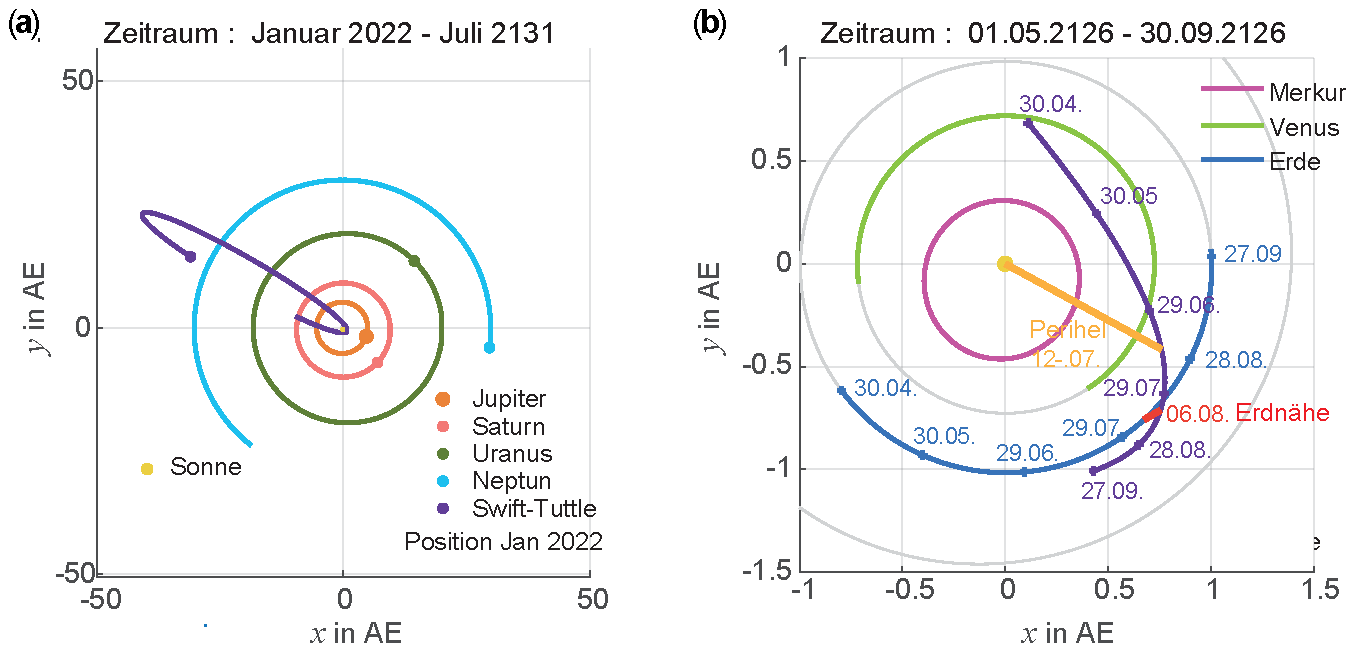
\includegraphics[width=\textwidth]{KometenKollision01.pdf}%
\caption[Trajektorien des Kometen Swift-Tuttle. ]{Berechnete Trajektorien des Kometen Swift-Tuttle. \fa Zeitraum 2022--2132  \fb Umgebung des Perihelduchgangs in 2126. Die Berechnung erfolgte durch numerische Integration der Bewegungsgleichungen \eqref{eq:hm_PlanetenDGLSystem01}.}
\label{abb:hm_SwiftTuttle01}%
\end{figure}

\begin{figure}[H]
\includegraphics[width=\textwidth]{KometenKollision02.pdf}%
\caption[Trajektorien des Kometen Swift-Tuttle zum Zeitpunkt Periheldurchgang in 2126.]{Berechnete Trajektorien des Kometen Swift-Tuttle zum Zeitpunkt des Periheldurchgangs in 2126. \fa Numerische Kepler-L�sung f�r den Kometen. \fb Numerische Integration der Bewegungsgleichungen \eqref{eq:hm_PlanetenDGLSystem01} �ber alle gr��eren Himmelsk�rper.}
\label{abb:hm_SwiftTuttle02}%
\end{figure}


\medskip \end{sol}

\textcolor{blue} {$\rightarrow$ zur} \probref{hm_Tempel1_SwiftTuttle}.\\
\noindent\rule[1ex]{\textwidth}{0.5pt} \newpage

%-----------------------------------------------------------------------------------------------------------

\begin{sol}{prob:hm_lichtlaufzeit}\label{lsg:hm_lichtlaufzeit} %�bung31
\textbf{Lichtlaufzeit, Unterschied $\ET-\UT$} \\ \\
Wir k�nnten zur L�sung der Aufgaben die verschiedenen \mscre zu den Kometen- und Asteroidenbahnen (\mlhmref{Kometenbahnen.m} und folgende) benutzen.
Wir wollen hier aber eine Absch�tzung machen und k�nnen uns daher das Leben etwas einfacher machen.
Wir nehmen an, dass Perihel und Perig�um in der ekliptikalen L�nge zusammenfallen und das beide in der Ekliptik liegen, \dh die ekliptikale Breite 0 ist.
Dies bedeutet, dass die Geschwindigkeit $v_\text{K}$ des Kometen maximal ist und ihre Richtung senkrecht zur Beobachtungsrichtung liegt.
Die Geschwindigkeit $v_\text{K}$ erh�lt man dann aus der vis-viva-Gleichung \eqref{eq:hm_vis-viva_polar} zu
	\[v_\text{K}^2=\mu_\text{G}\lk \frac{2}{q_\text{K}}-\frac{1}{a_\text{K}} \rk~,
\]
worin $q_\text{K}$ und $a_\text{K}$ der Perihelabstand bzw. die gro�e Halbachse der Kometenbahn sind.
Da f�r Kometen i.A. $a_\text{K}\gg q_\text{K}$ ist, gilt n�herungsweise
	\[v_\text{K} \approx \sqrt{\frac{2\mu_\text{G}}{q_\text{K}}} ~.
\]
Der Unterschied in astrometrischer und scheinbarer ekliptikaler L�nge ist dann gegeben durch:
	\[\Delta \lambda \approx \frac{v_\text{K} \Delta t}{q_\text{K}} = \frac{v_\text{K} (q_\text{K} /c)}{q_\text{K}} = \frac{1}{c} \sqrt{\frac{2\mu_\text{G}}{q_\text{K}}}.
\]
Unter der Annahme verschwindender ekliptikaler Breiten (siehe oben) und kleiner Zeiten $\Delta t$ k�nnen wir die Rektaszensions�nderung 
$\Delta \alpha$  aus der L�ngen�nderung  wie folgt 
	\[	\Delta \alpha = \Delta \lambda \cos \epsilon 
	\]
	berechnen, worin $\epsilon$ die Ekliptikschiefe ist.
        Wir erhalten dann f�r den Versatz auf der CCD in der Zwischenbildebene 
	\[\Delta x = \pm f \Delta \alpha ~~.
	\]
Das Bild des Kometen wird also dann im Bildfeld sein, wenn $\left| \Delta x \right| \leq 18 $ mm ist, wenn also gilt:
	\[\Delta x = \frac{f}{c} \sqrt{\frac{2\mu_\text{G}}{q_\text{K}}} \cos \epsilon \leq 18 \text{mm} 
	\]
Wir setzen f�r den Halleyschen Kometen (H) $q_\text{K} = 0.58 \text{AE}$ und f�r Neowise (N) $q_\text{K} = 0.29 \text{AE}$ ein und erhalten:
\begin{align*}
\Delta \alpha_\text{H} &= 0.58' ~~\text{ und } \Delta \alpha_\text{N} = 0.87'\\
v_\text{H}&= 55.3 \:\text{km/s} ~~\text{ und } ~v_\text{N} = 82.6\:\text{km/s}~\\
\Delta x_\text{H} &= 0.43\:\text{mm} ~~\text{ und } ~\Delta x_\text{N} = 0.63\:\text{mm}~,
\end{align*}
was merklich ist (30 Bogensekunden), aber noch deutlich innerhalb des Bildfeldes.
Folglich w�rde auch bei Benutzung von UT anstelle ET, was einer Lichtlaufzeit von ca. 1 min entspricht, ebenfalls ein messbarer Positionsfehler von ca. 6 bis 8 Bogensekunden entstehen, aber der Komet ebenfalls gut im Bildfeld sein.
F�r genaue Astronomie reicht die Nichtber�cksichtigung von $\Delta T$ nat�rlich nicht aus.
Wir berechnen jetzt die Zeit $\Delta t_\text{G}$ in der der Komet aus dem Bildfeld des mitgef�hrten Teleskops herauswandert.
Es gilt:
\[\Delta \alpha_\text{G} = \frac{18\:\text{mm}}{f} = \frac{v_\text{K} \Delta t_\text{G}}{\left| q_\text{K}-a_\text{earth}\right|} ~
\]
woraus f�r die beiden Zeiten 148 min bzw. 175 min folgt.
Das hei�t, dass selbst bei perfekt mitgef�hrtem Teleskop die Kometen nach zwei bis drei Stunden aus dem Teleskopbildfeld "`herauswandern"'.
Man kann also die Eigenbewegung der Kometen in einer Nacht sehr gut beobachten.
Die Rechnungen k�nnen nat�rlich auch im Detail mit dem \mscr~\mlhmref{Kometenbahnen.m} nachvollzogen werden. \\
\medskip \end{sol}
\textcolor{blue} {$\rightarrow$ zur} \probref{hm_lichtlaufzeit}.\\
\noindent\rule[1ex]{\textwidth}{0.5pt} \newpage

%-----------------------------------------------------------------------------------------------------------
\newpage
%%%-----------------------------------------------------------------------------------------------------------
\subsection{�bungen zu Gezeiten}

%-----------------------------------------------------------------------------------------------------------

\begin{sol} {prob:hm_rochelimit} \label{lsg:hm_rochelimit} %�bung32
\textbf{Zur Herleitung des Roche-Limits.}\\ \\

Wir benutzen Abb. 1.14 (Band I), wobei im Bild Sonne/Mond durch Jupiter ersetzt werden muss und die Erde durch den Kometen.
Ebenso ersetzen wir $m \rightarrow m_\text{K},\,r \rightarrow d,\, R_\text{E} \rightarrow R_\text{K}.$
Wir betrachten den Punkt ($x=0$, $y=0$, $z=-R_\text{K}$). Dann wird aus Gleichung (1.103) aus Band I:\footnote{Alternativ kann man nat�rlich auch direkt Gleichung (1.103) aus Band I mit $\theta = 0$ \bzw $\theta = \pi$ benutzen.} 

\begin{align}
    \vec{g}_z = -\frac{2G\,m_\text{J}}{d^3}\,R_\text{K}\,\vec{e}_z \,. \label{eq:hm_lsgroche02}
\end{align}
\begin{align}
    g_z = -g_\text{Gez,V} &= g_0\,\frac{R_\text{E}}{r}\lk 3\cos^2\theta-1\rk = \frac{3}{2}\,g_0\,\frac{R_\text{E}}{r}\lk \cos2\theta+\frac{1}{3}\rk \,. 
\end{align}

Andersereits wirkt an dem Punkt die (Selbst-) Gravitation des Kometen:
\begin{align}
    g_\text{K} = + \frac{G\,m_\text{K}}{R_\text{K}{}^2}\,\vec{e}_z \,. \label{eq:hm_lsgroche03}
\end{align}
von \eqref{eq:hm_lsgroche02} und \eqref{eq:hm_lsgroche03} ergibt die effektiv wirkende Gravitationsbeschleunigung $g_\text{eff}$ auf den Kometen:
\begin{align}
    g_\text{eff} = \frac{G\,m_\text{K}}{R_\text{K}{}^2}\,\lk 1-2\,\frac{m_\text{J}}{m_\text{K}}\,\frac{R_\text{K}{}^3}{d^3}\rk \,, \label{eq:hm_lsgroche04}
\end{align}
welche f�r
\begin{align}
    d = r_\text{R} = \sqrt[3]{2\,\frac{m_\text{J}}{m_\text{K}}}\,R_\text{K} \label{eq:hm_lsgroche05}
\end{align}
verschwindet. Das ist genau das Roche-Limit und der Komet wir bei diesem Abstand zerrissen. \\
F�r $m_\text{J}/m_\text{K}$ k�nnen wir auch schreiben 
\begin{align}
    \frac{m_\text{J}}{m_\text{K}} = \frac{\varrho_\text{J}}{\varrho_\text{K}}\,\frac{R_\text{J}{}^3}{R_\text{K}{}^3}\,,\label{eq:hm_lsgroche06}
\end{align}
womit aus \eqref{eq:hm_lsgroche05} folgt
\begin{align*}
    r_\text{R} = \sqrt[3]{2}\,\sqrt[3]{\frac{\varrho_\text{J}}{\varrho_\text{K}}}\,R_\text{J}\,.
\end{align*}
Mit den bekannten Werten $\varrho_\text{K} = \SI{500}{kg\per\cubic\metre}$, $\varrho_\text{J} = \SI{1333}{kg\per\cubic\metre}$ und $R_\text{J} = \SI{69911}{\km}$ ergibt sich
\begin{align*}
    r_\text{R,K} = 1.26\, \sqrt[3]{\frac{1.33}{0.5}}\,\SI{69911}{km} \approx \SI{122000}{\km}\,,
\end{align*}
was gut mit den beobachteten ca. $\SI{100000}{\km}$ zusammen passt.
Die Formel \eqref{eq:hm_lsgroche05} \bzw \eqref{eq:hm_lsgroche06} ergibt eher zu kleine Werte, da 
\begin{enumerate}
    \item [a)]
    der Komet als komplett fest und 
    \item [b)]
    auch dauerhaft kugelf�rmig bis zum Zerrei�en angenommen wurde. Tats�chlich wird sich dieser aber elongiert verformen und auch zumindest teilweise in einen fluiden Zustand �bergehen.  
\end{enumerate}
Der Radius der Hill-Sph�re des Jupiters betr�gt (\vgl \probref{hm_hill_sphere}) ca. $\SI{0.35}{}\,\mathrm{AE}$, also ein vielfaches des Roche-Limits. Himmelsk�rper k�nnen sich also lange im \anf{Einflussbereich} des Jupiters bewegen, bevor sie zerrissen werden. In \figref{hm_RocheLimit} haben wir die Hill-Sph�ren und die Roche-Limits f�r unser Sonnensystem graphisch dargestellt.
Wir verweisen auf \mlhmref{RocheLimit.m}.

\begin{table}[H] \caption{Roche-Limit und Hill-Sph�re in unserem Sonnensystem.}
\hspace{0.5cm}
\begin{tabular}{|R{1.25cm}|R{1.75cm}|R{1.25cm}|R{2cm}|R{1.75cm}|R{1.75cm}|R{1.5cm}|R{1.75cm}|}
\hline
\rule{0pt}{3pt}& & & & & & & \\
Planet   ~ & $a_\text{P}$ ~\linebreak in AE   ~ & $\varrho_\text{P}$ ~\linebreak in $\SI{}{\kg\per\metre\cubed}$ ~& Radius $R_\text{P}$ ~\linebreak in km  ~ & $m_\text{P}$ ~\linebreak in kg   ~& Roche-Limit ~\linebreak  in $\SI{}{\km}$ ~& Hill-Sph�re ~\linebreak in AE ~& Hill-Sph�re ~\linebreak in $\SI{}{\km}$ ~ \\
\rule{0pt}{3pt}& & & & & & & \\
\hline
\rule{0pt}{3pt}& & & & & & &\\
\rule{0pt}{6pt}Merkur  ~& $\SI{0.38709 }{}$    ~& $\SI{5 427}{}$ ~& $\SI{2 439}{}$ ~& $\SI{3.302e23}{}$ ~&  $\SI{6 806}{}$              ~& $\SI{0.001 }{}$            ~& $\SI{2.21e5 }{}$         ~\\
\rule{0pt}{6pt}Venus   ~& $\SI{0.72333}{}$     ~& $\SI{5 243}{}$ ~& $\SI{6 052}{}$  ~& $\SI{4.869e24}{}$ ~&  $\SI{16 691 }{}$            ~& $\SI{0.007}{}$             ~& $\SI{1.01e6  }{}$        ~\\
\rule{0pt}{6pt}Erde    ~& $\SI{1.00000}{}$     ~& $\SI{5 515}{}$ ~& $\SI{6 371}{}$  ~& $\SI{5.974e24}{}$ ~&  $\SI{17 869}{}$             ~& $\SI{0.010}{}$             ~& $\SI{1.50e6 }{}$         ~\\
\rule{0pt}{6pt}Mars    ~& $\SI{1.52366 }{}$    ~& $\SI{3 933}{}$ ~&$\SI{3 389}{}$   ~& $\SI{6.419e23}{}$ ~&  $\SI{8 494 }{}$             ~& $\SI{0.007 }{}$            ~& $\SI{1.08e6}{}$          ~\\
\rule{0pt}{6pt}Jupiter ~& $\SI{5.20336}{}$     ~& $\SI{1 326}{}$ ~& $\SI{69 911}{}$ ~& $\SI{1.899e27}{}$ ~&  $\SI{121 929  }{}$          ~& $\SI{0.355 }{}$            ~& $\SI{5.32e7 }{}$         ~\\
\rule{0pt}{6pt}Saturn  ~& $\SI{9.53707}{}$     ~& $\SI{687}{}$  ~& $\SI{58 233}{}$ ~& $\SI{5.685e26}{}$ ~&  $\SI{81 571}{}$             ~& $\SI{0.436 }{}$            ~& $\SI{6.52e7 }{}$         ~\\
\rule{0pt}{6pt}Uranus  ~& $\SI{19.19126}{}$    ~& $\SI{1 270}{}$ ~& $\SI{25 362}{}$ ~& $\SI{8.685e25}{}$ ~&  $\SI{43 601}{}$             ~& $\SI{0.469}{}$             ~& $\SI{7.01e7 }{}$         ~\\
\rule{0pt}{6pt}Neptun  ~& $\SI{30.06896}{}$    ~&$\SI{1 638 }{}$ ~& $\SI{24 622}{}$ ~& $\SI{1.026e26}{}$ ~&  $\SI{46 076}{}$             ~& $\SI{0.776 }{}$            ~& $\SI{1.16e8 }{}$         ~\\
\rule{0pt}{6pt}Pluto   ~& $\SI{39.48169}{}$    ~& $\SI{1 854}{}$ ~& $\SI{1 185}{}$  ~& $\SI{1.303e22}{}$ ~&  $\SI{2 311}{}$              ~& $\SI{0.051 }{}$            ~& $\SI{7.66e6}{}$          ~\\
\rule{0pt}{3pt}& & & & & & &\\
\hline
\end{tabular} \label{tab:hm_rochelimit}
\end{table}


\begin{figure}[H]
	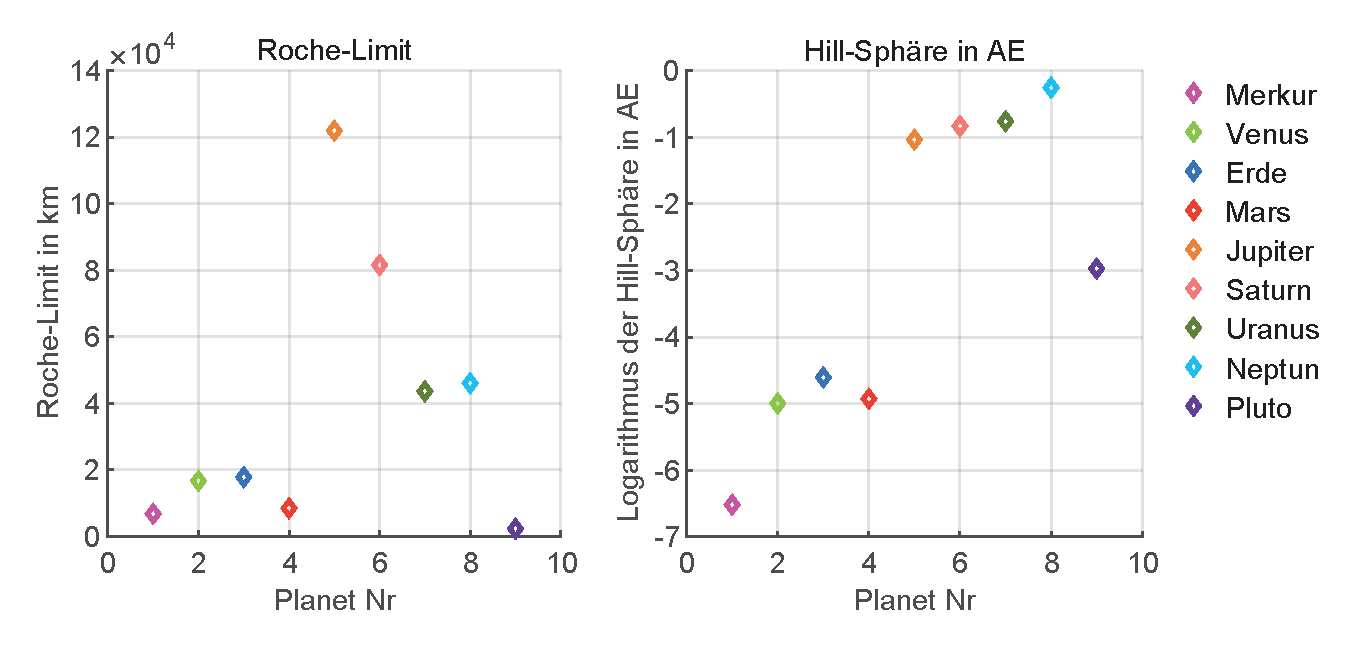
\includegraphics[width=\textwidth]{RocheLimit.pdf} 
	\caption[Vergleich Roche-Limit und Hill-Sph�re f�r unser Planetensystem.]{Vergleich Roche-Limit und Hill-Sph�re f�r unser Planetensystem.}
	\label{abb:hm_RocheLimit}
\end{figure}


\medskip \end{sol}
\textcolor{blue} {$\rightarrow$ zur} \probref{hm_rochelimit}.\\
\noindent\rule[1ex]{\textwidth}{0.5pt} \newpage


%-----------------------------------------------------------------------------------------------------------

\begin{sol} {prob:hm_gezeiten01} \label{lsg:hm_gezeiten01} %�bung33
\textbf{Tidenhub in einem Wasserglas}\\ \\

Wir betrachten \figref{hm_lsggezeiten01}. 
\begin{figure}[H]
	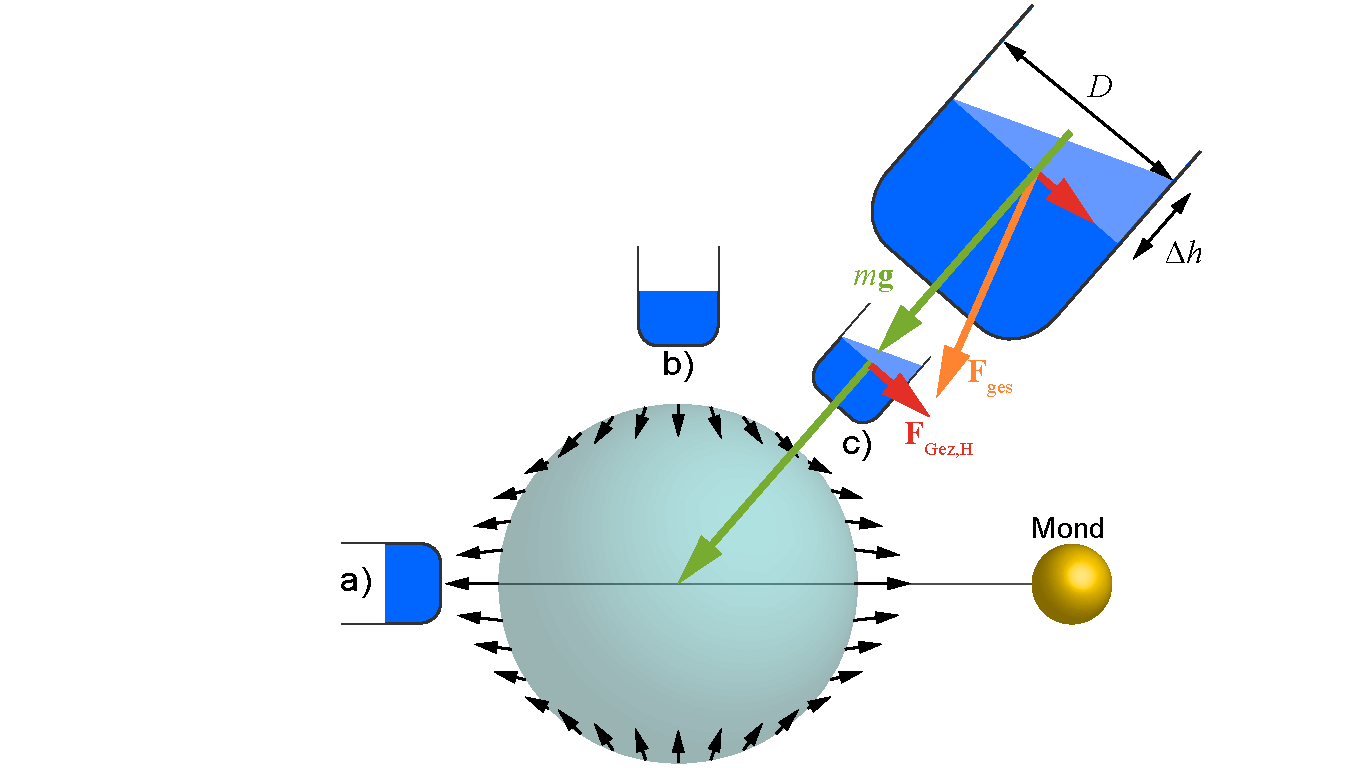
\includegraphics[width=\textwidth]{GezeitenWasserglas.pdf} 
	\caption{Gezeiten im Wasserglas}
	\label{abb:hm_lsggezeiten01}
\end{figure}
Nach der Gleichgewichtstheorie stellt sich die Wasseroberfl�che immer senkrecht zur resultierenden Gesamtschwerkraft $\vec{F}_\text{ges}$ ein. Der Tidenhub $\Delta h$ entspricht dann der Differenz der Wasserh�hen an beiden Ufern (\bzw dem R�ndern des Wasserglases). \\

Wir wollen nur die Wirkung des Mondes betrachten. Steht dieser im Zenit (Nadir) oder am Horizont, so bewirkt die resultierende Gesamtkraft keine Ver�nderung der Oberfl�che (Fall a,b). Im Fall c beginnt das Wasser durch Flie�en sich auszugleichen. \\
Der Tidenhub ergibt sich dann N�herungsweise zu:
\begin{align*}
    \Delta h = D\,\frac{F_\text{Gez,H}}{mg}\,.
\end{align*}
Wir wissen, dass $F_\text{Gez}/mg \approx \SI{e-7}{}$ ist, so dass folgt:
\begin{align*}
    \Delta h  &= \SI{e-8}{\metre} = \SI{10}{\nano\metre} ~~~~ \text{(Wasserglas)}, \\
    \Delta h  &= \SI{e-7}{}\cdot 5\cdot \SI{e4}{\metre} = 5\cdot \SI{e-3}{\metre} = \SI{5}{\mm} ~~~~ \text{(Bodensee)}.
\end{align*}

\newpage
Den Effekt im Glas k�nnte man im perfekt isolierten Labor ja noch interferometrisch messen, in der Badewanne oder aber im Bodensee wird er gegen�ber anderen Effekten verschwindend gering. 
In der Tat wurde die Wirkung von Gezeiten in $\SI{150}{\metre}$ langen Wasserrohren bereits 1914-1917 von Michelson\footnote{Albert Abraham Michelson (1852 -- 1931) war ein US-amerikanischer Physiker deutscher Herkunft. Er war einer der angesehensten Experimentalphysiker und wurde vor allem durch das nach ihm benannte Michelson-Interferometer bekannt. Er erhielt 1907 als erster US-Amerikaner den Nobelpreis f�r Physik.}\indexp{Michelson, Albert Abraham} und Mitarbeitern experimentell vermessen \cite{Michelson2014}.

\medskip \end{sol}
\textcolor{blue} {$\rightarrow$ zur} \probref{hm_gezeiten01}.\\
\noindent\rule[1ex]{\textwidth}{0.5pt} \newpage



%-----------------------------------------------------------------------------------------------------------

\begin{sol} {prob:hm_gezeiten02} \label{lsg:hm_gezeiten02} %�bung34
\textbf{Bewegung des Erdk�rpers im Erde-Mond-System.}\\

Der Umlauf von Erde und Mond um ihren gemeinsamen Schwerpunkt erzeugt oft Verwirrung. Oft wird argumentiert, dass die Erde dem Mond immer die gleich Seite zuwendet. Das ist aber falsch.
In der Realit�t f�hren alle Punkte der Erde eine Umlaufbewegung mit dem gleichen Radius aus und erfahren dabei eine gleiche Tr�gheitskraft (Fliehkraft), die immer vom Mond weg gerichtet ist. Jeder Punkt der Erde hat dabei sein eigenes Umlaufzentrum. Nur das gesamte System Erde-Mond f�hrt eine Bewegung um den Schwerpunkt S aus, nicht aber ein einzelner Massepunkt der Erde (Erde ist ja ein starrer K�rper).
Die \matlab{} Computersimulation \mlhmref{UmlaufErdeMond.m} zeigt in \figref{hm_lsggezeiten02}, dass jeder Punkt der Erde innerhalb eines synodischen Monats eine solche Kreisbewegung um sein jeweils eigenes "`Umlaufzentrum"' ausf�hrt. Dabei wurde die Situation f�r die �quatorebene dargestellt und angenommen, dass der Mond sich in der �quatorebene um den gemeinsamen Schwerpunkt S bewegt. Die Bewegung von zwei um $180\degree$ versetzten Punkten (T,B) in der �quatorebene sowie des Erdmittelpunktes im Lauf eines Monats sind dargestellt.

\newpage
\begin{figure}[H]
	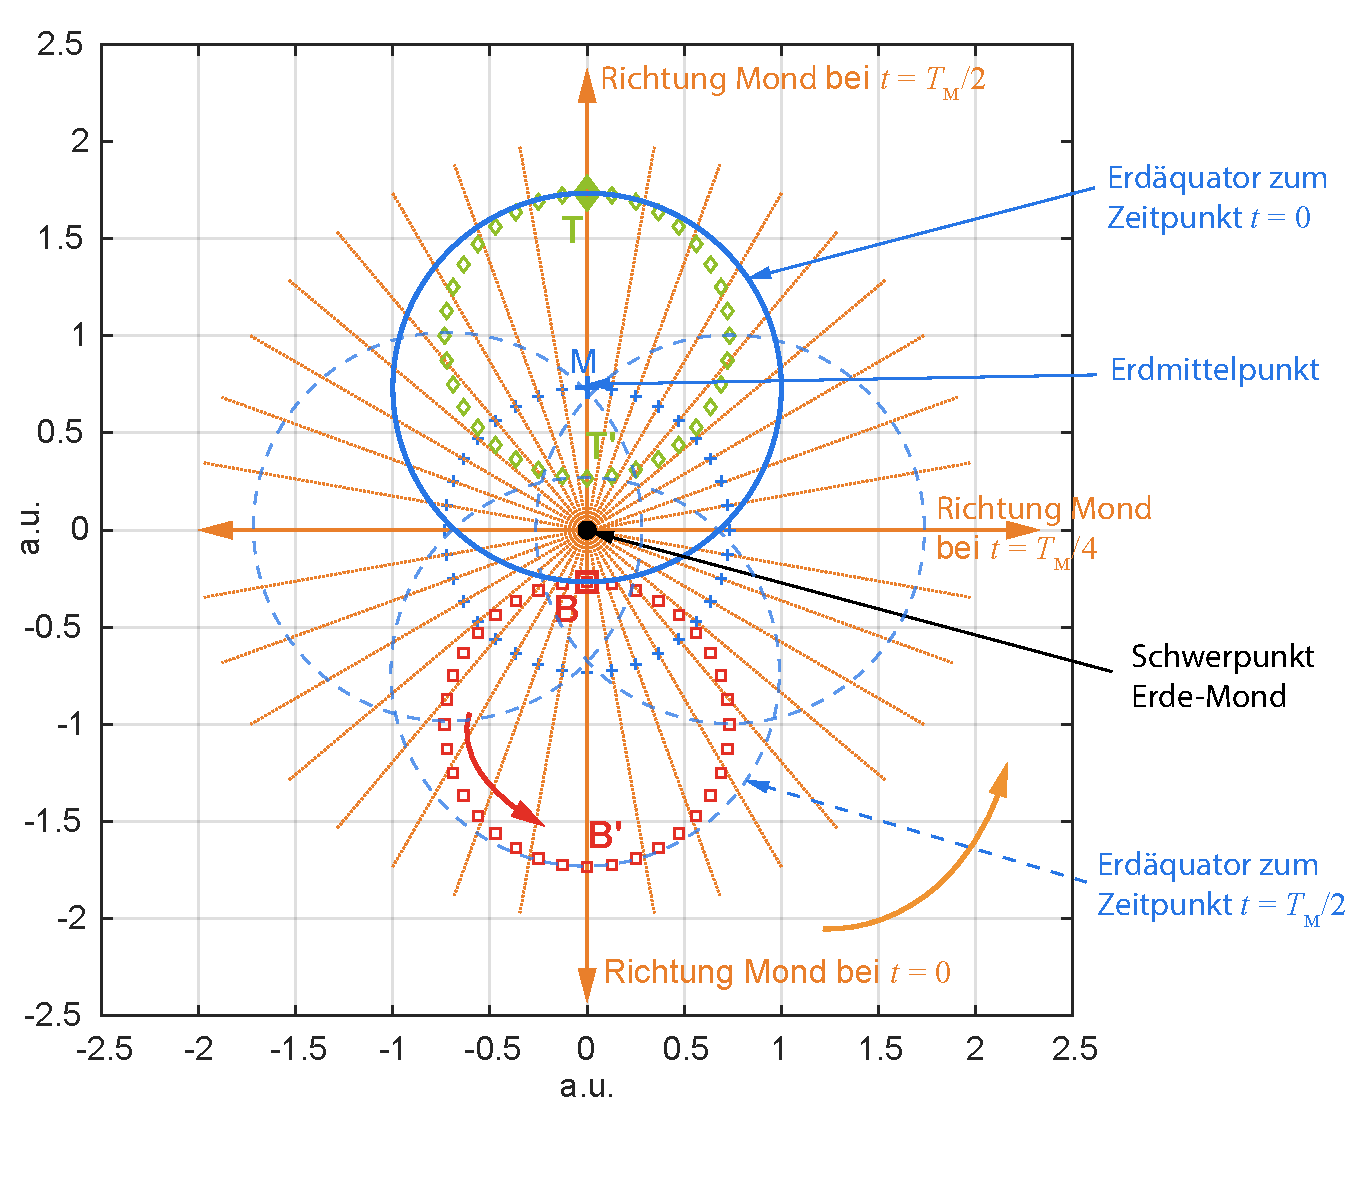
\includegraphics[width=\textwidth]{UmlaufErdeMond.pdf} 
	\caption[Bewegung von verschiedenen Punkten im Erde-Mond-System.]{Bewegung von verschiedenen Punkten der Erde bei einem Umlauf im Erde-Mond-Schwerpunkt-KOS. M ist der Erdmittelpunkt, T ein Punkt auf dem �quator, der bei $t=0$ auf der dem Mond abgewandten Seite liegt, T' der gleiche Punkt auf dem �quator, der bei $t=T_\text{M}/2$ dann auf der dem Mond zugewandten Seite liegt. F�r die Punkte B und B' gilt das Gleiche umgekehrt. $T_\text{M}$ ist die Umlaufzeit des Mondes um die Erde, die Erdrotation ist in dieser Betrachtung nicht ber�cksichtigt.}\label{abb:hm_lsggezeiten02}
\end{figure}
\end{sol}

\textcolor{blue} {$\rightarrow$ zur} \probref{hm_gezeiten02}.\\
\noindent\rule[1ex]{\textwidth}{0.5pt} \newpage

%-----------------------------------------------------------------------------------------------------------

\begin{sol} {prob:hm_gezeiten03} \label{lsg:hm_gezeiten03} %�bung35
\textbf{Newtonsche Gleichgewichtstheorie}\\ 

Abstand zwischen zwei Hochwassern und Tidenhub bei verschiedenen Deklinationen:
\begin{itemize}
	\item \textit{Abstand zwischen zwei Hochwassern }\\
			Aus der Dauer des synodischen Monats von $27.32 \mathrm{d}$ (Sonnentagen) ergibt sich eine mittlere Bewegung\index{Bewegung!mittlere} des Mondes von $n_\text{M} = 13.177\degree \mathrm{d}^{-1}$. An einem Sonnentag hat sich die Erde im Mittel um etwa 
	\[			360\degree \lk 1 + \frac{1\,\mathrm{d}}{365.25\,\mathrm{d}}\rk 
	\]
			weiter bewegt, was einer Bewegung von $n_\text{E} = 360.986\degree \mathrm{d}^{-1}$ entspricht. \\
			Wir wollen die zus�tzliche Zeit $\Delta T$ bestimmen, die verstreicht bis der Mond wieder im Meridian steht, \dh:
			\begin{align*}
					n_\text{E}\,\Delta T -360\degree &= n_\text{M} \, \Delta T \\
					\rightarrow ~~~~\Delta T = \frac{360\degree}{n_\text{E}-n_\text{M}} &= \frac{360\degree}{360.986\degree -13.177\degree}\, \mathrm{d} = \frac{360\degree}{347.809\degree}\, \mathrm{d} = 1.035 \mathrm{d} = \SI{24}{\hour}\,\SI{50}{\min}\,\SI{24}{\second}
			\end{align*}
			Hochwasser wird also im Mittel aller $\Delta T/2 = \SI{12}{\hour}\,\SI{25}{\min} $ eintreten.
			\begin{figure}%
			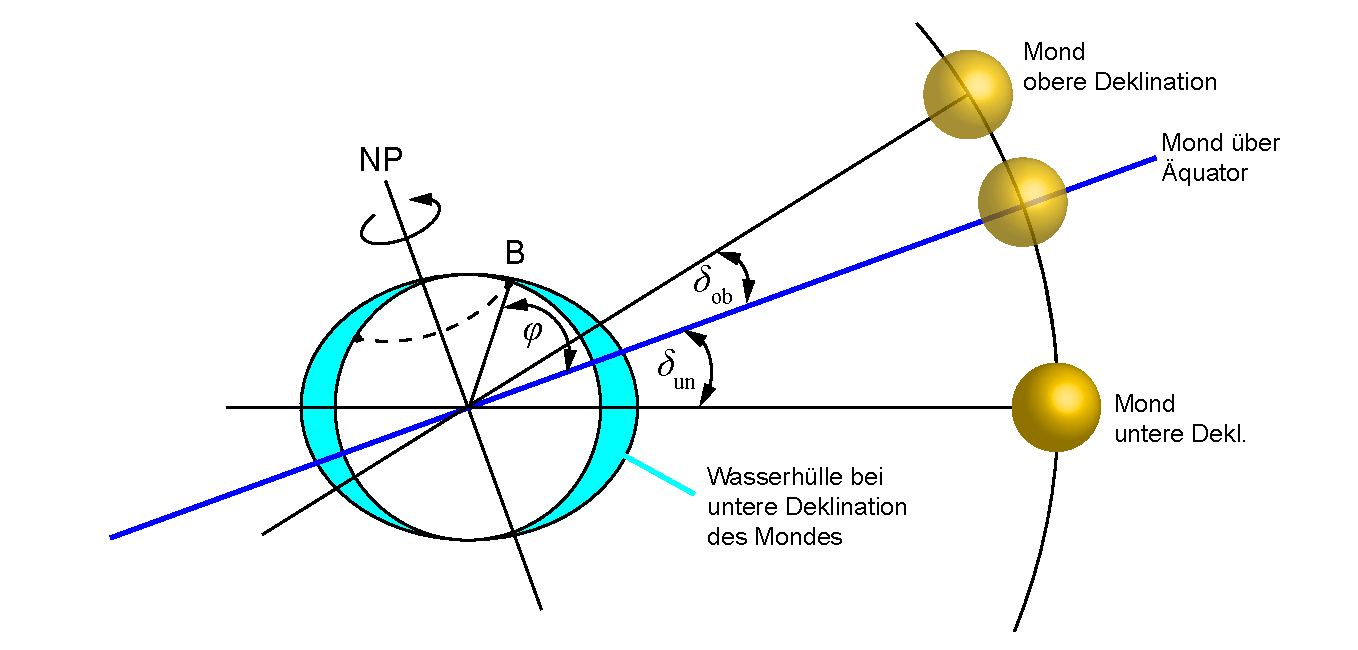
\includegraphics[width=\textwidth]{NewtonTheorieGez.pdf}%
			\caption{Anwendung der Newtonschen Gleichgewichtstheorie der Gezeiten}
			\label{abb:hm_lsggezeiten03}
			\end{figure}\newpage
	\item \textit{Tidenhub als Funktion der geographischen Breite }\\
	Man erkennt aus \figref{hm_lsggezeiten03}, dass die Tidenh�be f�r zwei aufeinander folgenden HW unterschiedlich hoch sind
	\item \textit{Tidenhub am �quator}\\
	Man erkennt aus \figref{hm_lsggezeiten03}, dass die Tidenh�be maximal sind, wenn der Mond die Deklination 0 hat. Ansonsten gibt es auch hier zwischen zwei aufeinander folgenden Hochwassern Unterschiede. Aus der Gezeitentabelle von Diego Garcia lesen wir heraus:
		\begin{enumerate}
		\item Sehr sch�n sind die Springtiden zum Vollmond und Neumond zu erkennen. (9.12. und 23.12.). Allerdings betr�gt die Differenz von HWH und NWH  \ca 250 cm, deutlich mehr als nach der Newtonschen Theorie zu erwarten w�re. Da zum Zeitpunkt des Vollmondes seine Deklination \ca $-10\degree$ betr�gt, die der Sonne \ca $-22\degree$ ist der Unterschied zwischen Tag- und Nachtiden entsprechend der unterschiedlichen Gezeitenwirkung ausgespr�gt. �hnliche Beobachtungen sind zur Neumondzeit zu machen.
		\item Der Mond kulminiert um \ca 9:00 Ortszeit, da finden wir aber NW, \dh wir haben fast eine Phasenverschiebung von $180\degree$, nach der Newtonschen Theorie nicht erkl�rbar.
		\item Die Nipptide am 15.12. ist gut ausgepr�gt, das Verh�ltnis von Spring- zu Nipptide von ca. 2.5 (250 cm / 100 m Tidenhub) entspricht grob der Newtonschen Theorie.
	\end{enumerate}
	\item
	  Die Nordsee ist ein sogenanntes Randmeer und bekommt daher die wesentlichen Gezeitenanregung vom Atlantik. Man kann sich die Nordsee als ein rechteckiges Becken von relativ geringer Tiefe (50 m) einer Breite/L�nge von etwa 1250 km vorstellen. Am Nordende dieses Beckens schwingen die Gezeitenwelle des Atlantiks mit Periode von $T = \SI{12}{\hour}\SI{25}{\minute}$ in das Becken nach S�den ein und werden an der Nordsee-S�dk�ste wieder reflektiert. Die Wellenl�nge berechnet sich aus $\lambda = c_\text{Welle} T = \sqrt{g\,h}\,T_\text{Gez}$ zu \ca 1000 km. Das Verh�ltnis zwischen Wellenl�nge und Beckenl�nge betr�gt somit etwa l : 1.25, bei diesem Schwingungsverh�ltnis bilden sich drei Schwingungsknoten aus (bei $\lambda=L$ w�ren es zwei.
    Durch die Coriolis-Kraft werden diese drei Schwingungsknoten zu ann�hernd station�ren amphidromischen Punkten, um die sich jeweils eine Welle im Gegenuhrzeigersinn bewegt. Man erkennt, dass diese amphidromischen Punkte nicht in der Mittelachse des Nordseebeckens liegen, sondern etwas nach Osten verschoben sind. Der Grund daf�r ist, dass die einlaufende Gezeitenwelle durch die geringe Tiefe der Nordsee stark abgebremst wird und so die wirkende Coriolis-Kraft Richtung S�den schw�cher wird. Diese asymmetrische Lage der amphidromischen Punkte ist f�r die unterschiedlich hohen Tidenh�be an Ost- und Westk�ste der Nordsee verantwortlich, da diese indirekt proportional zur Entfernung vom Amphidromiepunkt sind. (Je weiter weg, desto mehr kann sich die Gezeitenwelle aufbauen!).
\end{itemize}

\end{sol}
\textcolor{blue} {$\rightarrow$ zur} \probref{hm_gezeiten03}.\\
\noindent\rule[1ex]{\textwidth}{0.5pt} 

\begin{figure}%
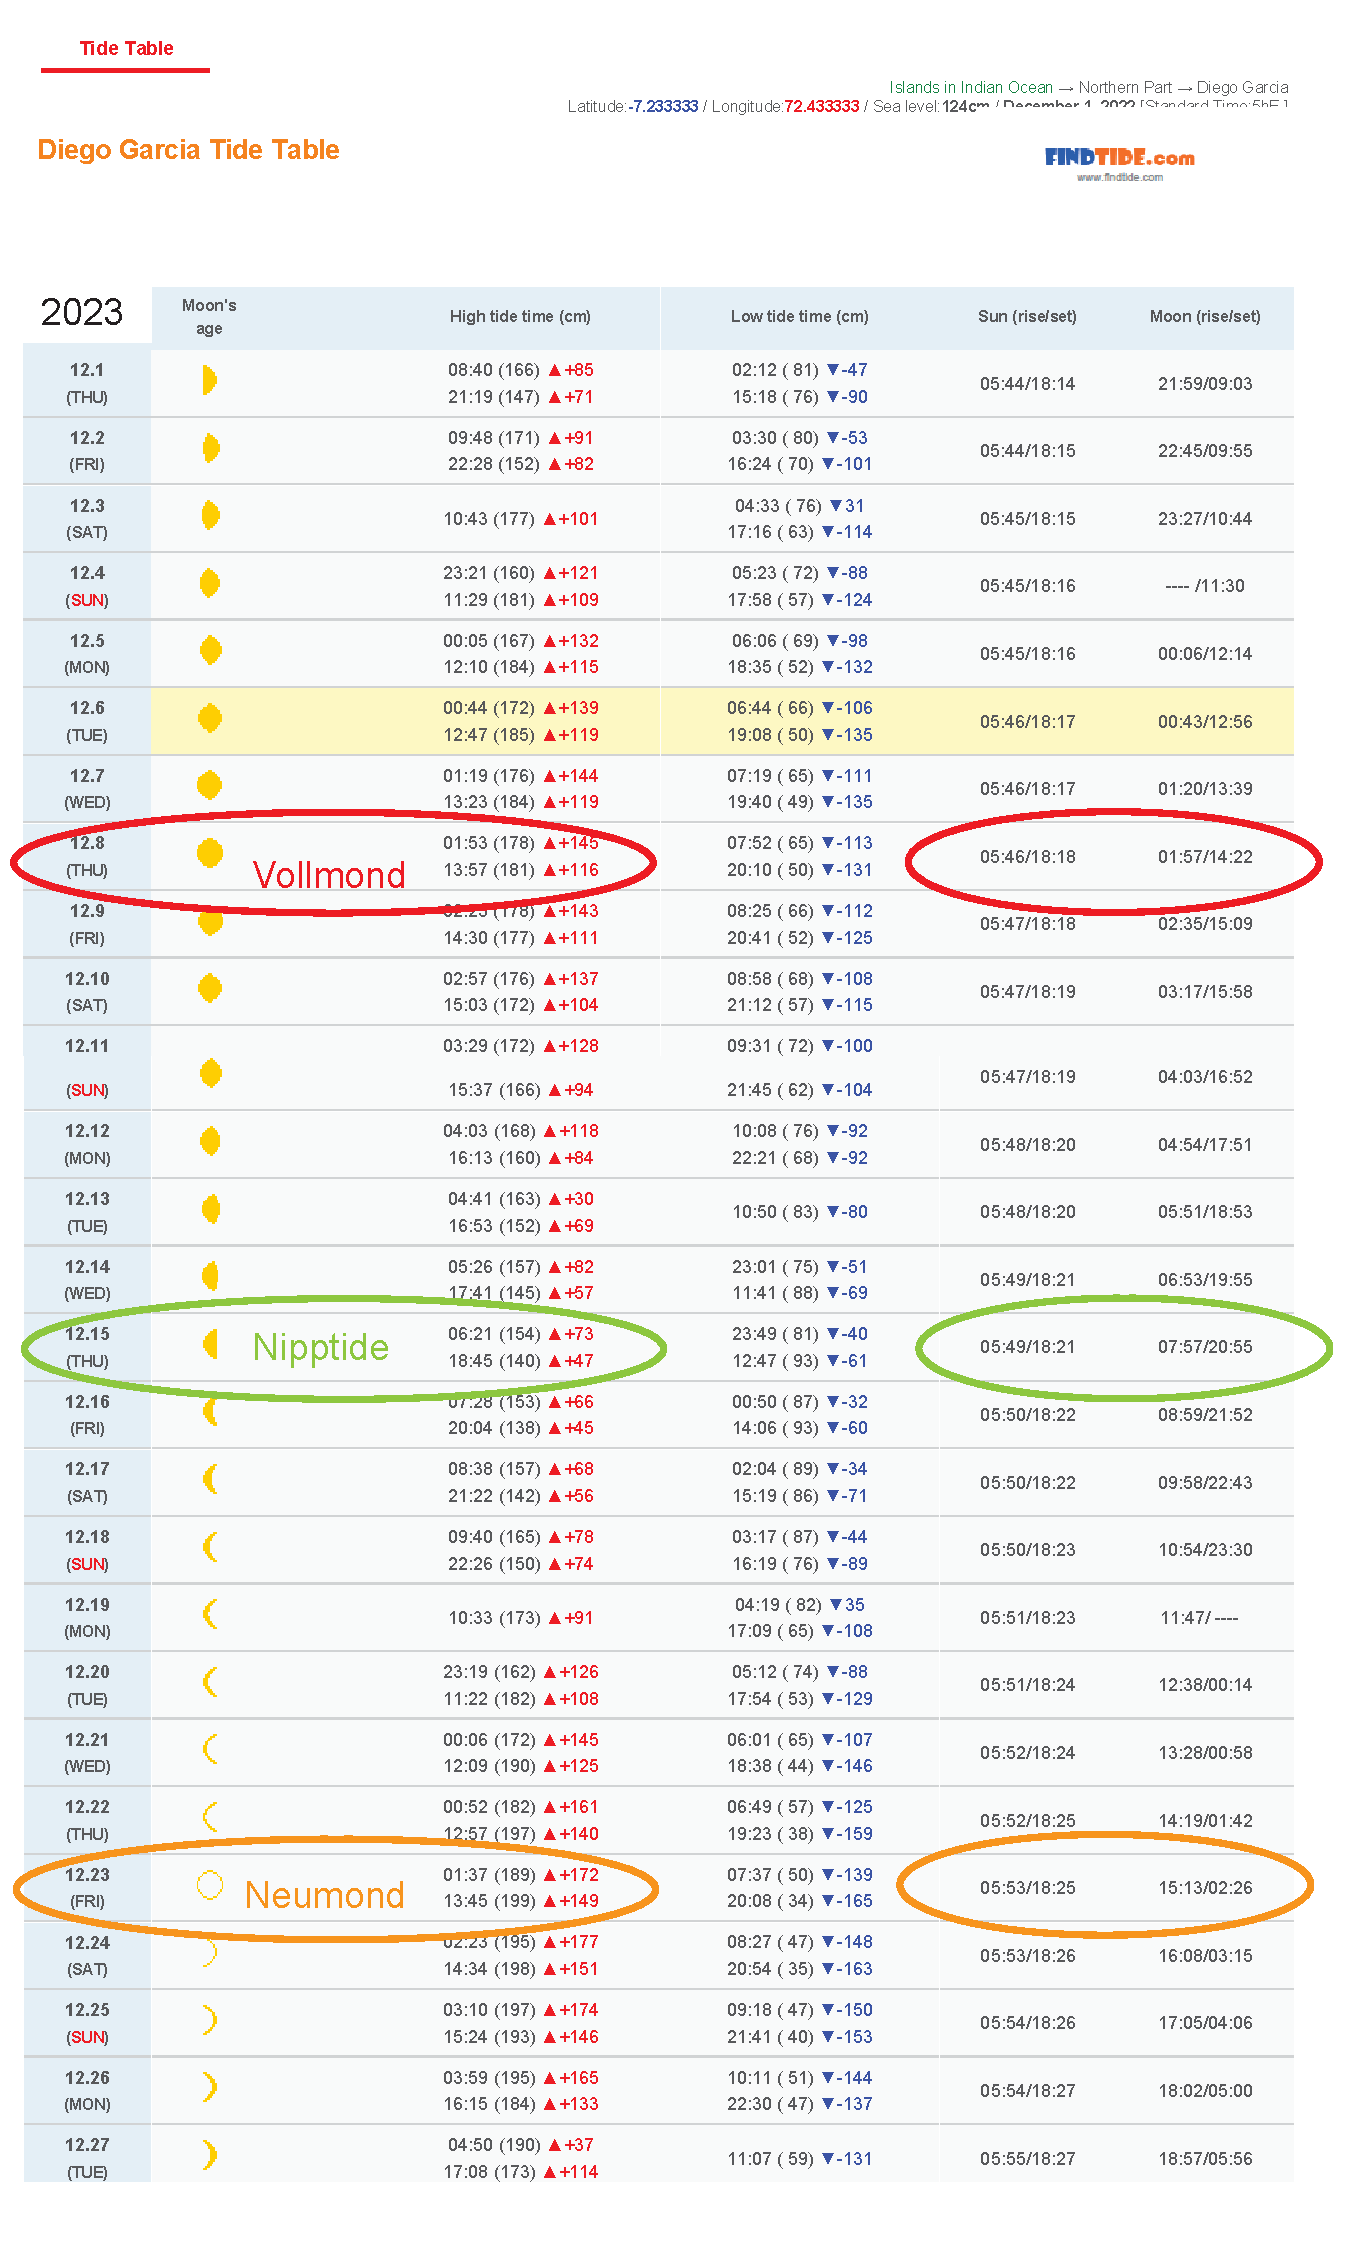
\includegraphics[width=\textwidth]{DiegoGarciaTideTableLsg.pdf}%
\caption{Tide Tabel von Diego Garcia im Indischen Ozean mit Beobachtungen}
	\label{abb:hm_DiegoGarciaTideTableLsg}
\end{figure}

\newpage

%-----------------------------------------------------------------------------------------------------------

\begin{sol} {prob:hm_gezeiten04} \label{lsg:hm_gezeiten04} %�bung36
\textbf{Gezeitenellipsoid}\\

\begin{itemize}
	\item \textit{\textbf{Newtonsche Gezeitentheorie}}\\ \\
	Wir verweisen auf \mlhmref{Gezeitenellipsoid.m}.

\begin{figure}[H]
	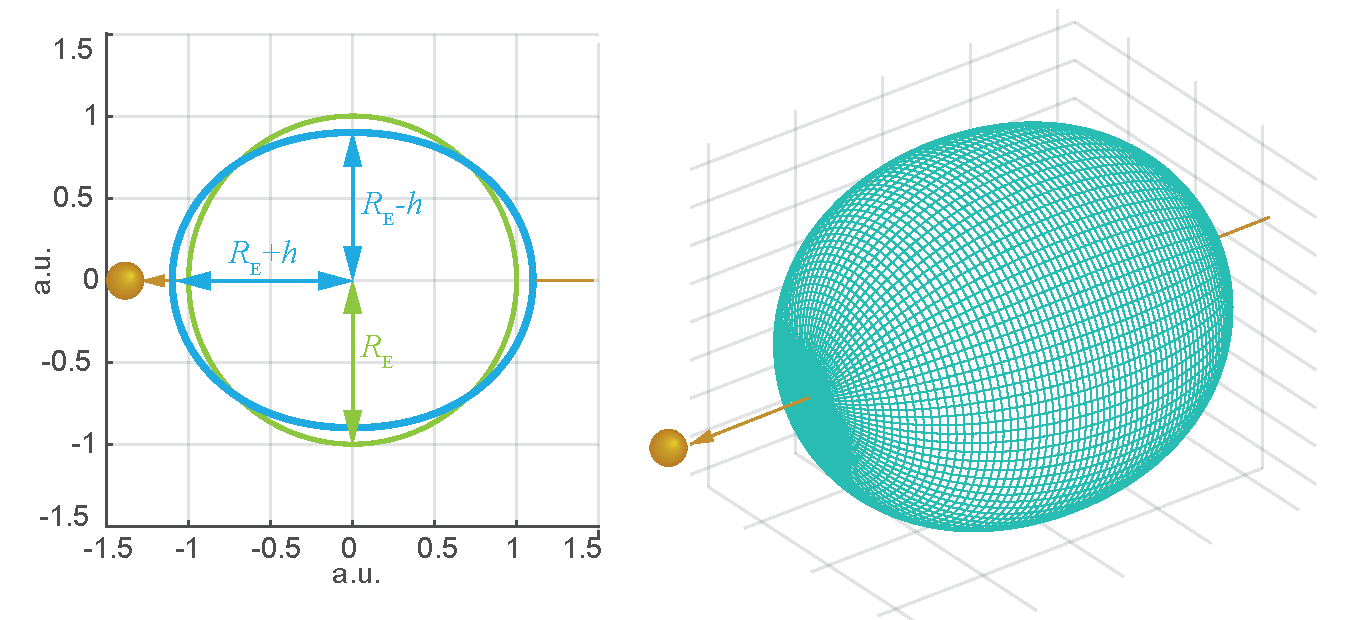
\includegraphics[width=\textwidth]{Gezeiten05.pdf} 
	\caption{Gezeitenellipsoid}
	\label{abb:hm_lsggezeiten04}
\end{figure}

F�r das Verh�ltnis der Volumina von Ellipsoid und Kugel finden wir :
	\[  \frac{V_\text{Ellip}}{V_\text{Kugel}} = \frac{(R_\text{E}+h)\,(R_\text{E}-h)^2}{R_\text{E}^3} \approx 1 - \frac{h}{R_\text{E}}  < 1\,,
	\]
was bedeutet, dass die angenommene Ellipsoidform nur eine N�herung sein kann. Eine verbesserte Rechnung m�sste sowohl die sogenannte Selbstgravitation des Gezeitenberges \cite{Norsen2017} als auch die Abflachungseffekte h�herer Ordnung sowie der bereits durch die Rotation der Erde hervorgerufene Abflachung \cite{Razmi2005} ber�cksichtigen.\\

	\item \textit{\textbf{Potentialtheorie}}\\ 

Wir benutzen \figref{hm_gezeiten02}. Das Potential der Gravitation des Mondes/der Sonne am Punkt $B$ ist gegeben durch: 
\begin{align*}
    U_\text{M} = -\frac{G\,m_\text{M}}{r'} ~~~~ \text{\bzw} ~~~~ U_\text{S} &= -\frac{G\,m_\text{S}}{r'}\,.
\end{align*}
Wir entwickeln $\vec{r}'= \vec{r} -\vec{R}$ wieder wie in \kap{hm_potentialtheorie} in sph�rischen Koordinaten $r,\theta$ (unter Ausnutzung der Rotationssymmetrie) und erhalten aus:
\begin{align}
    \frac{1}{r'} &= \frac{1}{\sqrt{r^2-2\vec{r}\,\vec{R} + R^2}} = \frac{1}{\sqrt{r^2-2r\,R\,\cos\theta+R^2}}  \label{eq:hm_lsggez31}\,.
\end{align}
Wir setzen jetzt $r= a_\text{EM}$ als festen Abstand der Mittelpunkte von der Erde und Mond und erhalten aus \eqref{eq:hm_lsggez31} wieder eine Entwicklung nach den Legendre-Polynomen analog zu \eqref{eq:hm_pot_theo07}
\begin{align}
    \frac{1}{r'} = \frac{1}{a_\text{EM}} \sum\limits_{n=0}^\infty \lk \frac{r}{a_\text{EM}}\rk^n\,\PL n\,\lk \cos\theta\rk\,. \label{eq:hm_lsggez32}
\end{align}
Daraus folgt mit $\mu_\text{M} = Gm_\text{M}$ das Potential am Punkt $B$ der Erdoberfl�che zu:
\begin{align}
    U_\text{M} = -\frac{\mu_\text{M}}{a_\text{EM}}\lek 1+\frac{r}{a_\text{EM}}\,\PL 1 \,\lk \cos\theta\rk + \frac{r^2}{{a_\text{EM}{}^2}}\,\PL 2 \,\lk\cos\theta\rk\rek\label{eq:hm_lsggez33}
\end{align}
und analog f�r die Sonne, wobei wir im Folgenden nun den Mond betrachten. \\
Der betrachtete Punkt $B$ erf�hrt im mitrotierenden Erde-Mond-System eine Zentrifugalkraft \bzw -Beschleunigung (siehe \probref{hm_gezeiten02})
\begin{align*}
    \vec{g}_\text{Z} &= -\omega_\text{M}{}^2\,\frac{m_\text{M}}{m_\text{M}+m_\text{E}} \,a_\text{EM}\,\vec{e}_\text{Z} \\
    &\approx -\omega_\text{M}\,\frac{m_\text{M}}{m_\text{E}}\,a_\text{EM}\,\vec{e}_\text{Z} = -\vec{\nabla}\,U_\text{Z}\,.
\end{align*}
Dies kann man mit \figref{hm_gezeiten02} als Potential
\begin{align}
    U_\text{Z} = \omega^2\,\frac{m_\text{M}}{m_\text{E}}\,a_\text{EM}\,r\,\cos\theta\label{eq:hm_lsggez34}
\end{align}
schreiben.\\
Wir benutzen, dass $\PL 1 \,\lk\cos\theta\rk = \cos\theta$ ist und erhalten mit $\omega^2 = \frac{\mu_\text{M}}{a_\text{EM}{}^3}$ (3. Keplersches Gesetz)
\begin{align}
    U_\text{Z} = \frac{\mu_\text{M}}{a_\text{EM}}\,\frac{r}{a_\text{EM}}\,\PL 1\,\lk\cos\theta\rk \label{eq:hm_lsggez35}\,.
\end{align}
Das gesamte auf den mitbewegten Punkt $B$ wirkende Potential ist dann die Summe von $U_\text{Z}$ und $U_\text{M}$, woraus folgt:
\begin{align}
    U = U_\text{Z} + U_\text{M} = -\frac{\mu_\text{M}}{a_\text{EM}}\,\lek 1+\frac{r^2}{a_\text{EM}{}^2}\,\PL 2\,\lk\cos\theta\rk\rek \,. \label{eq:hm_lsggez36}
\end{align}
Man erkennt aus \eqref{eq:hm_lsggez36}, dass sich die Terme, die linear in $r$ \bzw $\cos\theta$ sind, wegheben (bedingt durch die Balance von Gravitation und Zentrifugalkraft im rotierenden Erde-Mond-System) und dass als Zusatzterm zum Monopolpotential einer Punktmasse in 2. Ordnung das Gravitationspotential proportional zu $a_\text{EM}{}^{-3}$ �brig bleibt. \\ \\
Eine Fl�ssigkeit auf der Erdoberfl�che stellt sich in der H�he $h\lk\theta\rk$ und hat damit ein Potential $g\,h\lk\theta\rk$. Das gesamte Potential ist dann:
\begin{align}
    U_\text{total}\lk\theta\rk = -\frac{G\,m_\text{M}}{a_\text{EM}} + g\,h\lk\theta\rk- \zeta\,g\,\PL 2\,\lk\cos\theta\rk \label{eq:hm_lsggez37}
\end{align}
worin $\zeta$ durch
\begin{align*}
    \zeta = \frac{R_\text{E}{}^3}{a_\text{EM}{}^3}\,\frac{m_\text{M}}{m_\text{E}}\,R_\text{E}
\end{align*}
gegeben ist und wir $g= G\,m_\text{E}/r_\text{E}{}^2$ benutzt haben. \\
F�r eine Fl�ssigkeit muss das Potential $U$ unabh�ngig von $\theta$ sein, weil es sonst zu Ausgleichsstr�men kommt, womit sofort 
\begin{align}
    h\lk\theta\rk=\zeta\,\PL 2\,\lk\cos\theta\rk \label{eq:hm_lsggez38}
\end{align}
folgt und damit das bereits aus \eqref{eq:hm_gezeiten16} bekannte Ergebnis (bis auf konstante Terme).\\
In dieser Herleitung haben wir eine Fl�ssigkeit mit der Dichte $0$ unterstellt, die eine Erde die absolut fest ist komplett bedeckt. \\
Ein besseres Modell w�re sicher ein Zwei-Komponenten-Modell aus einem Planeten mit mittlerem Radius $R_\text{E}$, der einen homogenen inkompressiblen Ozean der Dichte $\rho_\text{W}$, einen homogenen, festen Kern der Dichte $\rho_\text{K}$ und eine Steifigkeit $\mu$ hat. Um dieses Modell zu berechnen, muss man die Effekte des Gravitationsfeldes des Gezeitenellipsoids selbst (die sogenannte Eigengravitation) und die der elastischen Kr�fte im Kern ber�cksichtigen. 
Wir verweisen %auf das erweiterte Problem in \probref{hm_gezeiten_zusatz} und 
die Spezialliteratur \cite{Murray2008,Norsen2017}.

\end{itemize}

\medskip \end{sol}
\textcolor{blue} {$\rightarrow$ zur} \probref{hm_gezeiten04}.\\
\noindent\rule[1ex]{\textwidth}{0.5pt} \newpage

%-----------------------------------------------------------------------------------------------------------

\begin{sol} {prob:hm_gezeiten05} \label{lsg:hm_gezeiten05} %�bung37
\textbf{Wasserkanal nach Airy \cite{Butikov2001}.}\\ \\

Einfaches Modell zur Dynamischen Theorie: 
Wir beziehen uns auf die instruktive Darstellung in \cite{Butikov2001}.
Wir betrachten den Airy-Wasserkanal entlang des �quators um die Erde und eine erzwungene Gezeitenschwingung (elliptischer Form) $q_1(t)$, deren Hauptachse auf die Erde-Mond-Linie ausgerichtet ist. Eine weitere Gezeitenschwingung (elliptischer Form), deren Hauptachse um $45\degree$ zur Erde-Mond-Linie verdreht ist, sei durch $q_2(t)$ gegeben. Die erzwungenen Wasserschwingungen im Kanal haben eine Eigenfrequenz $\omega_\text{Welle}$, die im Wesentlichen durch die Kanaltiefe bestimmt ist (siehe Band I) und die durch die halbt�gliche Gezeitenanregung mit $\omega_\text{Gez} = 2\,\omega_\text{E}$ erzwungen werden:
\begin{align*}
	\ddot{q}_1 +2\gamma\,\dot{q}_1 + \omega_\text{Welle}^2\,q_1 = A_1\,\omega_\text{Welle}^2\,\cos(\omega_\text{Gez}t) \,, \\
  \ddot{q}_2 +2\gamma\,\dot{q}_2 + \omega_\text{Welle}^2\,q_2 = A_2\,\omega_\text{Welle}^2\,\sin(\omega_\text{Gez}t)  \,.
\end{align*}
Hierin sind $\gamma$ die D�mpfungen und $A_, A_2 $ die Amplituden der Anregung der Gezeitenwellen.
Die Wasserh�hensteigung im Kanal an einer beliebigen Stelle des �quators (gegeben durch $R_\text{E},\, \theta$) ist dann gegeben durch:
	\[\Delta h = q_1\lk t\rk \cos 2\theta + q_2\lk t\rk \sin 2\theta \,.
	\]
F�r den Fall einer extrem langsam rotierenden Erde ist die Wasserh�hensteigung durch die station�re L�sung  $q_i(t)$ gegeben durch, wobei wir die Amplituden $A_1,\,A_2$ f�r beide Gezeitenwellen gleich annehmen wollen:
\begin{align}
   \Delta h &= q_1\lk t\rk \cos 2\theta + q_2\lk t\rk \sin 2\theta  \nonumber \\
    &= A\lek \cos\lk 2\omega_\text{Gez}t \rk \, \cos 2\theta + \sin \lk 2\omega_\text{Gez}t \rk \,\sin 2\theta \rek  \nonumber \\
    &= A\, \cos \lk 2\lk \omega_\text{Gez}t-\theta\rk\rk\,,  \label{eq:hm_gezeitenlsg01}
\end{align}
was bedeutet, dass die elliptischen Gezeitenverformungen der langsam rotierenden Erde folgen. Die Hauptachse der Gezeitenellipse ist immer auf die Erd-Mond-Linie ausgerichtet. \\
F�r beliebige $\omega_\text{E}$ benutzen wir als L�sung f�r die $q_i\lk t\rk$ die Berechnungen f�r den getriebenen Oszillator nach Gleichung (1.165) aus Kapitel 1.3.2 (Band I) mit der Amplitude
\begin{align*}
     \hat{q} &= \frac{\omega_\text{Gez}\,A}{\sqrt{\lk \omega_\text{Welle}{}^2\, - \,\omega_\text{Gez}{}^2\rk^2 + 4\gamma^2\,\omega_\text{Gez}{}^2}} \,,
\end{align*} 
und der Phase
\begin{align*}
    \delta &= \arctan\lek \frac{2\gamma\,\omega_\text{Gez}}{\omega_\text{Welle}{}^2 - \omega_\text{Gez}{}^2}\rek \,.
\end{align*} 
Daraus folgt nun f�r den Wasserh�henanstieg im Kanal:
\begin{align}
   \Delta h &= q_1\lk t\rk \cos 2\theta + q_2\lk t\rk \sin 2\theta  \nonumber \\
            &= \hat{q}\,\lek \cos\lk 2\omega_\text{E}t-\delta\rk\,\cos 2\theta + \sin\lk 2\omega_\text{E}t-\delta\rk\,\sin 2\theta\rek \nonumber \\
            &= \hat{q}\,\cos\lek 2\,\lk \omega_\text{E}t-\delta/2-\theta\rk\rek \,. \label{eq:hm_gezeitenlsg02}
\end{align}
Man erkennt aus \eqref{eq:hm_gezeitenlsg02}, dass der HW-Zeitpunkt an einer bestimmten Stelle des Erd�quators $R_\text{E},\, \theta$ gegeben ist durch:
\begin{align*}
    \theta_\text{max} = \omega_\text{E}\,t - \frac{\delta}{2}\,,
\end{align*}
was bedeutet, dass das Hochwasser mit einer bestimmten Zeitverschiebung  $\delta/2$ gegen�ber der Kulmination des Mond eintritt. Diese Verschiebung h�ngt von der Eigenfrequenz $\omega_\text{Welle}$ der Gezeitenwelle und ihrer D�mpfung $\gamma$ ab. In \figref{hm_lsggezeiten05} haben wir die �berlagerung und Verschiebung zur Erde Mond-Linie dargestellt.
Eine Simulation findet sich in \mlhmref{SimulationAiry.m}.

\begin{figure}[H]
	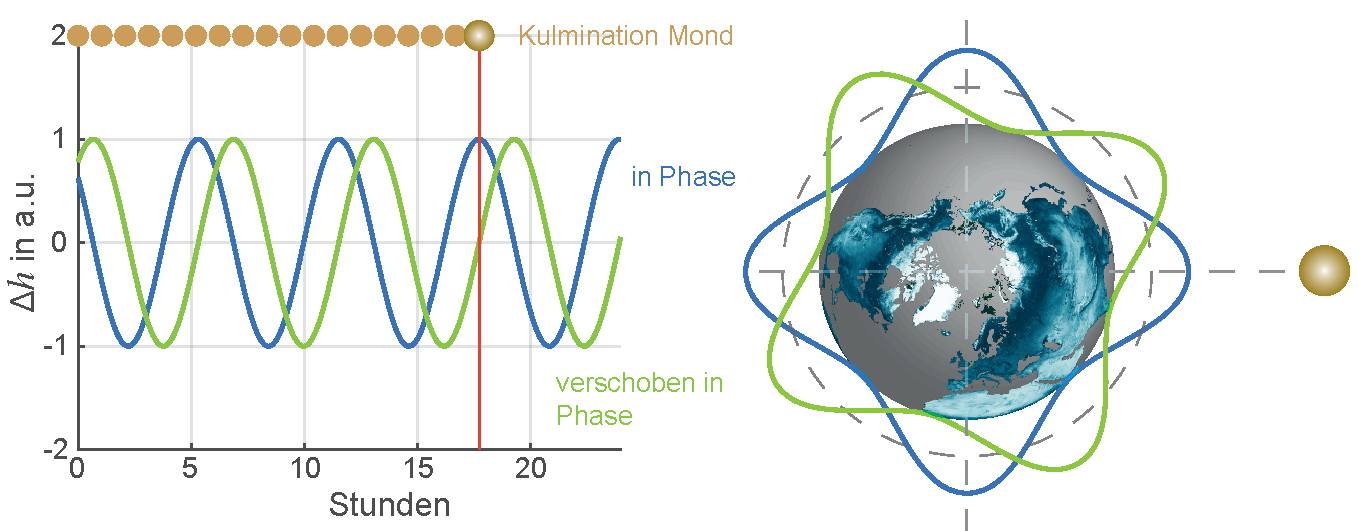
\includegraphics[width=\textwidth]{SimulationAiry.pdf} 
	\caption[Einfaches Modell zur Dynamischen Theorie.]{Einfaches Kanal-Modell nach Airy zur dynamischen Theorie der Gezeiten. Siehe auch \mlhmref{SimulationAiry.m}.
}
	\label{abb:hm_lsggezeiten05}
\end{figure}


\medskip \end{sol}
\textcolor{blue} {$\rightarrow$ zur} \probref{hm_gezeiten05}.\\
\noindent\rule[1ex]{\textwidth}{0.5pt} \newpage

%-----------------------------------------------------------------------------------------------------------

\begin{sol} {prob:hm_gezeiten06} \label{lsg:hm_gezeiten06} %�bung38
\textbf{Gezeitenreibung Hantelmodell}\\ \\

Die Rechnungen sind im Detail im \mscr{} \mlhmref{GezeitenReibung02.m} hinterlegt.
\begin{figure}[H]
	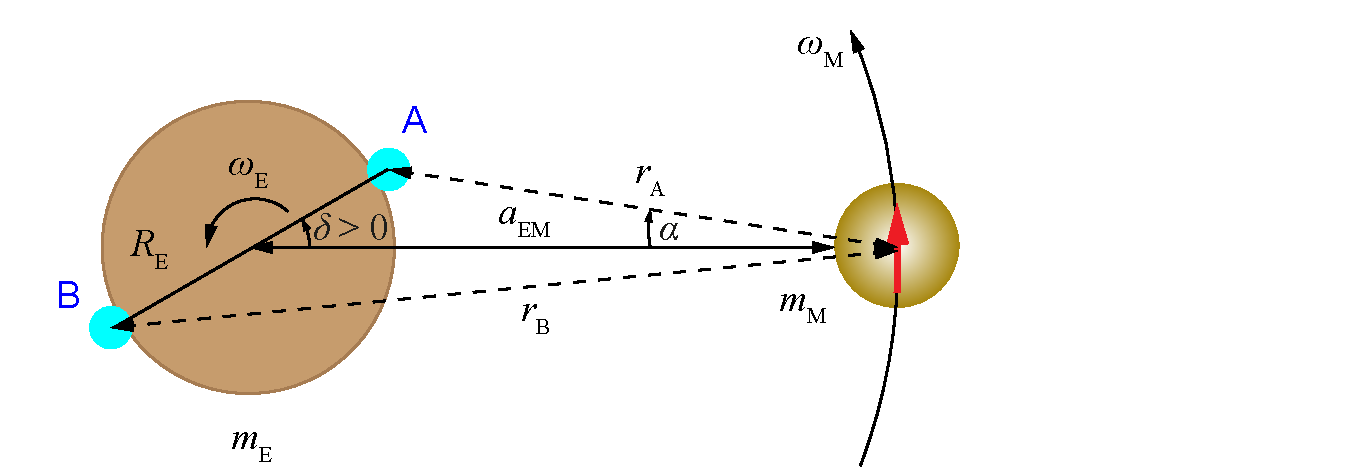
\includegraphics[width=\textwidth]{GezeitenHantel.pdf} 
	\caption{Gezeitenreibung - Hantelmodell}
	\label{abb:hm_lsggezeiten06}
\end{figure}
F�r die Berechnungen geben wir folgende Hinweise und Vorgehensweise zun�chst zur Ableitung des Drehmomentes aus \figref{hm_lsggezeiten06} an:
\begin{enumerate}
    \item [1)] Als erstes berechnen wir die Drehimpulse f�r den heutigen Zustand (Wir lassend dabei den Index 0 weg.):
    \begin{align*}
        L_\text{E} &= J_\text{E}\,\omega_\text{E}\,,~~ J_\text{E}\, \text{wird sp�ter berechnet}\,,~~~ \omega_\text{E} = \frac{2\pi}{\SI{86125}{\second}} \\
        L_\text{M} &= J_{\text{M}}\,\omega_\text{M} = m_\text{M}\,a_\text{EM}{}^2\,\omega_\text{M}\,, ~~~\omega_\text{M} = \frac{2\pi}{T_\text{synod.}}\,.
    \end{align*}
    %2)
    \item [2)] In der finalen Situation gilt: $\omega_\text{E,f} = \omega_\text{M,f}$:
    \begin{align*}
        L_\text{E,f} &= J_\text{E}\,\omega_\text{E,f}~,~~  L_\text{M,f} = J_\text{M,f}\,\omega_\text{M,f} = m_\text{M}\,a_\text{EM,f}{}^2\,\omega_\text{M,f}\,.
		\end{align*}
    %3)
    \item [3)] Aus der Drehimpulserhaltung folgt:
    \begin{align*}
        L_\text{ges} = J_\text{E}\,\omega_\text{E} + J_\text{M}\,\omega_\text{E} = J_\text{E}\,\omega_\text{E,f} + J_\text{M,f}\,\omega_\text{M,f}\,
    \end{align*}
und mit
    \begin{align*}
        \omega_\text{E,f} &= \omega_\text{M,f} ~~\rightarrow~~J_\text{E}\,\omega_\text{E} + J_\text{M}\,\omega_\text{M} = \lk J_\text{E} + J_\text{M,f}\rk\,\omega_\text{M,f}\,.
    \end{align*}
    Wir vergleichen:
    \begin{align*}
        J_\text{E} &\approx \frac{2}{5}\,m_\text{E}\,R_\text{E}{}^2\,~~\text{und}~~ J_\text{M,f} > J_\text{M} = m_\text{M}\,a_\text{EM}{}^2 ~\rightarrow~
        \frac{J_\text{E}}{J_\text{M}} = \frac{2}{5}\,\frac{m_\text{E}}{m_\text{M}}\,\frac{R_\text{E}{}^2}{a_\text{EM}{}^2} = 0.0045 \ll 1\,.
    \end{align*}
    Deswegen k�nnen wir in guter N�herung $J_\text{E} \ll J_\text{M,f}$ annehmen, womit folgt:
    \begin{align}
        L_\text{ges} = J_\text{E}\,\omega_{\text{E}} + J_\text{M}\,\omega_\text{E} = J_\text{M,f}\,\omega_\text{M,f} \label{eq:hm_gezUebg01} \,.
    \end{align}
    %4)
    \item[4)] Wir bestimmen nun den endg�ltigen Erde-Mond-Abstand $a_\text{EM,f}$ und die endg�ltige Kreisfrequenz $\omega_\text{M,f}$. Dazu betrachten wir die Kr�ftebilanz im finalen Zustand:
    \begin{align}
        \frac{G\,\killA{m_\text{M}}\,m_\text{E}}{a_\text{EM,f}{}^2} = \killA{m_\text{M}}\,\omega_\text{M,f}{}^2\,a_\text{EM,f} \label{eq:hm_gezUebg02} \,.
    \end{align}
    Aus \eqref{eq:hm_gezUebg01} und \eqref{eq:hm_gezUebg02} folgt
    \begin{align}
        a_\text{EM,f} &= \frac{L_\text{ges}{}^2}{G\,m_\text{E}\,m_\text{M}{}^2} \label{eq:hm_gezUebg03} \\
        \omega_\text{M,f} &= \frac{L_\text{ges}}{m_\text{M}\,a_\text{EM,f}{}^2} = \frac{G^2\,m_\text{E}{}^2\,m_\text{M}{}^3}{L_\text{ges}^3}\,. \label{eq:hm_gezUebg04}
    \end{align}
    %5)
    \item [5)] Zur Berechnung von $L_\text{ges}$ brauchen wir noch das Tr�gheitsmoment der Erde. \\
    Wir wollen die Erde aus einem Kern mit Dichte $\varrho_\text{K}$ und Radius $R_\text{K}$ und einer Schale $\varrho_\text{S}$ im Radiusbereich $R_\text{U}$ bis $R_\text{E}$ annehmen.
    \begin{align*}
        J_\text{E} &= \frac{2}{5}\,\lk \frac{4}{3}\,\pi\,\varrho_\text{S}\,R_\text{E}{}^3\rk\,R_\text{E}{}^2 + \frac{2}{5}\,\lk \frac{4}{5}\pi\,\lk \varrho_\text{K}-\varrho_\text{S}\rk\,R_\text{K}{}^3\rk\,R_\text{K}{}^2 \\
        &= \frac{2}{3}\,\frac{4}{3}\,\pi\lek \varrho_\text{S}\,R_\text{E}{}^5 + \varrho_\text{K}\,R_\text{K}{}^5 - \varrho_\text{S}\,R_\text{K}{}^5\rek = \frac{8}{15}\,\pi\lek \varrho_\text{S}\,\lk R_\text{E}{}^5 -R_\text{K}{}^5\rk + \varrho_\text{K}\,R_\text{K}{}^5\rek \\
        &\approx \SI{7.83e37}{\kg\square\metre}\\
        \text{\vgl homogene Erde} ~~~~ J_\text{EK} &= \frac{8}{15}\,\pi\,\varrho_\text{E}\,R_\text{E}{}^5 = \SI{9.7e37}{\kg\square\metre} \,.
    \end{align*}
    %6)
    \item[6)] Damit erhalten wir
    \begin{align*}
        L_\text{ges} &= J_\text{E}\,\omega_\text{E} + J_\text{M}\,\omega_\text{M} \approx \SI{3.45e34}{\kg\square\metre\per\second}\,.
    \end{align*}
    %7)
    \item[7)] Aus \eqref{eq:hm_gezUebg03} und \eqref{eq:hm_gezUebg04} erhalten wir:
    \begin{align*}
        a_\text{EM,f} &= \SI{5.55e8}{\km} = 1.44\,a_\text{EM}\,~~\text{und}~~ \omega_\text{M,f} = \SI{1.528e-6}{\per\second} ~~\rightarrow ~~T_\text{E,f} = \frac{2\pi}{\omega_\text{M,f}} = \SI{47.59}{}~\mathrm{d}\,.
    \end{align*}
    %8)
   \item [8)] Jetzt wollen wir noch wissen, wie lange es dauert bis der finale Zustand erreicht ist, \bzw um welche Distanz sich der Mond pro Jahrhundert entfernt. Nach \figref{hm_lsggezeiten06} ist:
    \begin{align*}
        F_\text{A} = \frac{G\,m\,m_\text{M}}{r_\text{A}{}^2} &= \frac{G\,m\,m_\text{M}}{a_\text{EM}{}^2 + R_\text{E}{}^2 - 2a_\text{EM}\,R_\text{E}\,\cos\delta} \\
        F_\text{B} = \frac{G\,m\,m_\text{M}}{r_\text{B}{}^2} &= \frac{G\,m\,m_\text{M}}{a_\text{EM}{}^2 + R_\text{E}{}^2 - 2a_\text{EM}\,R_\text{E}\,\cos\lk 180\degree-\delta\rk} \\
        &= \frac{G\,m\,m_\text{M}}{a_\text{EM}{}^2 + R_\text{E}{}^2 + 2a_\text{EM}\,R_\text{E}\,\cos\delta }
    \end{align*}
    Die Drehmomente auf die Hantel ergeben sich f�r kleine Winkel $\delta$ und $\alpha\approx 0$ zu:
    \begin{align*}
						\vec{M}_\text{D, A} &= \vec{R}_\text{E} \times \vec{F}_\text{A}\\
						M_\text{D, A}  &= R_\text{E}\,F_\text{A}\,\lk -\cos\delta\,\sin\alpha - \sin\delta\,\cos\alpha \rk \\
						\sin\delta &\approx \delta,~~\alpha \approx \frac{R_\text{E}}{r_\text{A}}\delta~\text{Sinussatz}\,~~~ \cos\alpha \approx 1,~~ \cos\delta \approx 1\,,\\
						M_\text{D, A}  &= +R_\text{E}\,F_\text{A}\,\delta \lk 1 + \frac{R_\text{E}}{r_\text{A}} \rk \,,~~
						M_\text{D, B}  = -R_\text{E}\,F_\text{B}\,\delta \lk 1 - \frac{R_\text{E}}{r_\text{A}} \rk \,, \\
						\rightarrow ~~M_\text{D, ges}&\approx -R_\text{E}\delta \lk F_\text{A} - F_\text{B} \rk \,.
			\end{align*}
    F�r das Gesamtdrehmoment auf die Hantel nehmen wir f�r $m$  \ca $\SI{e-8}{}$ $m_\text{E}$ an (wegen $g_\text{gez}|g_\text{E}$) also $m\approx\SI{3.8e-16}{\kg}$, $\delta = 3\degree$ 
    \begin{align*}
        \rightarrow ~~~~  M_\text{D, ges} &= \SI{-4.39e16}{\N\metre}
    \end{align*}
    %9)
    \item[9)] 
		Die Bewegungsgleichung f�r den starren K�rper ergibt:
    \begin{align*}
        -\frac{\D L}{\D t}\,M &=  M_\text{D, ges} = \frac{\D L_\text{E}}{\D t} = J_\text{E}\,\dot{\omega}_\text{E} = \frac{\D }{\D t}\,\lk m_\text{M}\,\omega_\text{M}\,a_\text{EM,f}{}^2\rk
    \end{align*}
    Aus der Drehimpulserhaltung folgt:
    \begin{align*}
				L &= \frac{2}{5}\,m_\text{E}\,R_\text{E}{}^2\,\omega_\text{E} + m_\text{M}\,a_\text{EM}{}^2\,\omega_\text{M} \\
				\frac{\D L}{\D t} = 0 &= \frac{2}{5}\,m_\text{E}\,R_\text{E}{}^2\,\dot{\omega}_\text{E} + 2m_\text{M}\,a_\text{EM}\,\dot{a}_\text{EM}\,\omega_\text{M} + m_\text{M}\,a_\text{EM}{}^2\,\dot{\omega}_\text{M} ~~~~ \Bigg|\substack{:\lk 2m_\text{M}\,a_\text{EM}{}^2\,\omega_\text{M} \rk}\\					0 &= \frac{1}{5}\,\frac{m_\text{E}\,R_\text{E}{}^2}{m_\text{M}\,a_\text{EM}{}^2}\,\frac{\dot{\omega}_\text{E}}{\omega_\text{M}} + \frac{\dot{a}_\text{EM}}{a_\text{EM}} + \frac{1}{2}\,\frac{\dot{\omega}_\text{M}}{\omega_\text{M}} \\
					\omega_\text{M} &= \sqrt{G\,m_\text{M}}\,a_{EM}{}^{-\frac{3}{2}} ~~~~ \rightarrow ~~~~ \dot{\omega}_\text{M} = \sqrt{G\,m_\text{M}}\,\lk -\frac{3}{2}\rk\,a_\text{EM}{}^{-\frac{5}{2}}\,\dot{a}_\text{EM} = -\frac{3}{2}\,\frac{\dot{a}_\text{EM}}{a_\text{EM}}\,\omega_\text{M} \\
				\rightarrow ~~~~ &-\frac{1}{5}\,\frac{m_\text{E}\,R_\text{E}{}^2}{m_\text{M}\,a_\text{EM}{}^2}\,\frac{\dot{\omega}_\text{E}}{\omega_\text{M}} = \frac{\dot{a}_\text{EM}}{a_\text{EM}}\,\lk 1-\frac{1}{2}\,\frac{3}{2}\rk \\
				\rightarrow ~~~~ &\frac{\dot{a}_\text{EM}}{a_\text{EM}} = -\frac{4}{5}\,\frac{m_\text{E}\,R_\text{E}{}^2}{m_\text{M}\,a_\text{EM}{}^2}\,\frac{\dot{\omega}_\text{E}}{\omega_\text{M}}\\
        \rightarrow ~~~~ &\dot{\omega_\text{E}} = \frac{M_\text{ges}}{J_\text{E}} \approx \SI{-5.61e-22}{\per\square\second} \,, \\
        \rightarrow ~~~~ &\dot{a}_\text{EM} = -2\,\frac{J_\text{E}\,\dot{\omega}_\text{E}}{m_\text{M}\,a_\text{EM}\,\omega_\text{M}} \approx \SI{1.17e-9}{\metre\per\second}\,.
    \end{align*}
    Umgerechnet bedeutet das f�r 100 Jahre:
    \begin{align*}
        \Delta T_\text{PE} &= -\frac{\dot{\omega}_\text{E}}{2\pi}\,T_\text{PE}{}^2\, \underbrace{100 \cdot 365 \cdot 86400}_{\substack{=100\,\mathrm{a}}} \SI{}{\second} = -\frac{\dot{\omega}_\text{E}}{\omega_\text{E}{}^2}\,2\pi\, 100\,\mathrm{a} \approx \SI{0.0021}{} \SI{}{\second} = \SI{2.1}{\metre\second}\,, \\
        \Delta a_\text{EM} &= \dot{a}_\text{EM}\, 100\,\mathrm{a} \approx \SI{3.7}{\metre}\,.
    \end{align*}
    %10)
\end{enumerate}

Jetzt wollen wir uns noch die Energiebilanz anschauen. Wir geben auch dazu die Vorgehensweise an:
    \begin{align*}
         E_\text{ges} &= \frac{J_\text{E}}{2}\,\omega_\text{E}{}^2 + \frac{J_\text{M}}{2}\,\omega_\text{M}{}^2 - \frac{G\,m_\text{M}\,m_\text{E}}{a_\text{EM}}\,,\\
         E_\text{ges} &= \frac{J_\text{E}}{2}\,\omega_\text{E}{}^2 + \frac{J_\text{M}}{2}\,\frac{G\,m_\text{E}}{a_\text{EM}{}^3} - \frac{G\,m_\text{M}\,m_\text{E}}{a_\text{EM}}\,, \\
        \rightarrow\frac{\D E}{\D t} &= J_\text{E}\,\omega_\text{E}\,\dot{\omega}_\text{E} - \frac{3}{2}\,\frac{J_\text{M}\,G\,m_\text{E}}{a_\text{EM}{}^4}\,\dot{a}_\text{EM} + \frac{G\,m_\text{E}\,m_\text{M}}{a_\text{EM}{}^2} \,\dot{a}_\text{EM} = P_\text{V} \approx \SI{-3.3e12}{\W}\,.
    \end{align*}
    Wir berechnen die \anf{Arbeit}, die die Gravitationsenergie beim Anheben der Ozeane leistet (pro Tag). Dazu brauchen wir zun�chst die Masse $m_\text{W}$ der angehobenen Wasserschicht:
    \begin{align*}
        m_\text{W} &= \frac{4}{3}\,\pi\,\lk R_\text{E} +h\rk^3\,\varrho - \frac{4}{3}\,\pi\,R_\text{E}\,\varrho = \frac{4}{3}\,\pi\,\varrho\,R_\text{E}{}^3\,\lk 1 + \frac{3h}{R_\text{E}} + \killA{\mathcal{O} \lk \frac{h^2}{R_\text{E}{}^2}\rk}\rk \,,\\
        \rightarrow ~ E_\text{W} &= -2m_\text{W}\,g\,h = \SI{-2.5e18}{\W} \,,\\
        P_\text{Diss} = \dot{E}_\text{Diss} &= -10\% \, \frac{E_\text{W}}{\SI{24}{\hour}} = \SI{-2.9e12}{\W} \,, \\
        E_\text{Diss} \lk 1a\rk &= P_\text{Diss} \, 1a = \SI{-25.4}{\peta\W\hour} = \SI{-25.4e4}{\tera\W\hour} \,.
    \end{align*}
    Wir vergleichen das mit dem weltweiten Prim�renergieverbrauch 2021 von 600 ExaJoule = $\SI{1.67e5}{\tera\W\hour}$, was bedeutet, dass die Gezeitenreibungs-Verlustenergie etwa $10\%$ des weltweiten Prim�renergieverbrauchs betr�gt. Wir k�nnen noch absch�tzen, zu welcher Erw�rmung der Ozeane das f�hrt, falls keine Abstrahlung ins Weltall erfolgen w�rde.
    \begin{align*}
        E_\text{Diss}\lk 1a\rk &= m_\text{W}\,c\,\Delta T~,~~~c_\text{W} = \SI{4.2}{}\,\frac{\SI{}{\kilo\J}}{\SI{}{\kg\K}}\,,\\
        \Delta T_\text{W} &= \frac{E_\text{Diss}\lk 1a\rk}{m_\text{W}\,c_\text{W}} \approx \SI{0.8}{\K} \,.
     \end{align*}

\medskip \end{sol}
\textcolor{blue} {$\rightarrow$ zur} \probref{hm_gezeiten06}.\\
\noindent\rule[1ex]{\textwidth}{0.5pt} \newpage

%-----------------------------------------------------------------------------------------------------------

\begin{sol}{prob:hm_gezeiten06a}\label{lsg:hm_gezeiten06a} %�bung39
\textbf{Gezeitenreibung - Auswirkung Mond.}\\ \\

Wir k�nnen die gleichen Gedankeng�nge wie im \kap{hm_gezeitenreibung} machen und erhalten die entsprechenden Gleichungen angepasst f�r den Mond.\\
Insbesondere ergibt \eqref{eq:hm_gezreibung08} nun:
\begin{align*}
    \frac{\dot{\Omega}_\text{M}}{\Omega_\text{M}} &= -\frac{45}{4}\,\frac{\omega_\text{M}{}^2}{\omega_\text{M}}\,\frac{m_\text{E}}{m_\text{M}}\,\lk \frac{R_\text{M}}{a_\text{EM}}\rk^3\,\frac{\delta}{1+\tilde{\mu}} \\
    &\approx \SI{1.1e-14}{\per\second}
\end{align*}
Die Zeitdauer, in der der Mond auf eine synchrone Eigenrotation gekommen ist, betr�gt dann
\begin{align*}
    \Delta T \approx \Big|\frac{\Omega_\text{M}}{\dot{\Omega}_\text{M}}\Big| \approx \SI{3e6}{} \text{Jahre}\,.
\end{align*}
Im Vergleich zum angenommenen Mondalter von ca. 4.5 Milliarden Jahren ist das eine verschwindend kurze Zeit. Daher ist es kaum �berraschend, dass der Mond schon lange eine synchrone Rotation zur Erde hat und uns immer das gleiche Gesicht zeigt.

\medskip \end{sol}
\textcolor{blue} {$\rightarrow$ zur} \probref{hm_gezeiten06}.\\
\noindent\rule[1ex]{\textwidth}{0.5pt} \newpage

%-----------------------------------------------------------------------------------------------------------

\begin{sol}{prob:hm_gezeiten07}\label{lsg:hm_gezeiten07} 
\textbf{Gravitationspotential au�erhalb eines Rotationsellipsoids.}\\ %�bung40

Wir nehmen die Form des homogenen Rotationsellipsoids mit
\begin{align}
    r'\lk \theta'\rk = R_0\lk 1-\frac{2}{3}\,\epsilon\,\PL 2\,\lk \cos\theta'\rk\rk \label{eq:hm_rotell01}
\end{align}
an, wobei $|\epsilon|\ll 1$ sein soll. \\
Nach \eqref{eq:hm_pot_theo07} in \kap{hm_pot_rotsymm_distrib} k�nnen wir das Potential an einem Ort $r,\, \theta$ vschreiben als:
\begin{align}
    U\lk r,\theta\rk = \sum_{n=0}^\infty \Phi_n\,\frac{\PL n \,\lk \cos\theta\rk}{r^{n+1}}\,, \label{eq:hm_rotell02}
\end{align}
worin
\begin{align}
    \Phi_n = -2\pi\,G\,\int\limits_0^\pi\int\limits_0^{r'\lk\theta'\rk}\,r'^{2+n}\,\varrho\lk r',\theta'\rk\,\PL n\lk\cos\theta'\rk \,\sin\theta'\,\D r'\,\D \theta'\,. \label{eq:hm_rotell03}
\end{align}
Das Integral ist �ber die gesamte Masseverteilung desK�rpers zu nehmen. \\
F�r einen homogenen K�rper der Dichte $\varrho$ k�nnen wir schreiben:
\begin{align}
    \Phi_n = -2\pi\,G\,\varrho\int\limits_0^\pi \PL n\,\lk\cos\theta'\rk \int\limits_0^{r'\lk \theta'\rk}r'^{2+n}\,\D r' \,\sin\theta'\,\D \theta'\,. \label{eq:hm_rotell04}
\end{align}
Die Integration �ber $r'$ ergibt:
\begin{align}
    \Phi_n = -\frac{2\pi\,G\,\varrho}{\lk n+3\rk}\int\limits_0^\pi \PL n\,\lk\cos\theta'\rk \,\lek r'\lk\theta'\rk\rek^{n+3}\,\sin\theta'\,\D \theta' \label{eq:hm_rotell05}\,,
\end{align}
in welches wir \eqref{eq:hm_rotell01} einsetzen und somit erhalten:
\begin{align}
    \Phi_n\approx -\frac{2\pi\,G\,\varrho}{\lk n+3\rk} \int\limits_0^\pi \PL n\,\lk \cos\theta'\rk R_0{}^{n+3}\,\lek \PL 0\lk\cos\theta'\rk - \frac{2}{3}\,\lk n+3\rk\,\epsilon\,\PL 2\lk\cos\theta'\rk\rek\,\sin\theta'\,\D \theta'\,. \label{eq:hm_rotell06}
\end{align}
Hier haben wir f�r $|\epsilon|\ll 1$\, $\lk 1+\epsilon\, x\rk^{n+3} \approx 1 + \lk n+3\rk\,\epsilon\, x$ und ferner $\PL 0\,\lk \cos\theta'\rk = 1$ benutzt.\\
Wegen der Orthogonalit�t der Legendre-Polynome (siehe \cite{Riley2006, Olver1992, Fischer2018} und die \onlineZ) k�nnen nur $\Phi_0$ und $\Phi_2$ von Null verschieden sein. Wir erhalten:
\begin{align}
\begin{split}
    \Phi_0 &= -\frac{4\pi\,G\,\varrho\,R_0{}^3}{3} = -G\,M\,, \\
    \Phi_2 &= \frac{8\pi\,G\,\varrho\,R_0{}^5\,\epsilon}{15} = \frac{2}{5}\,G\,M\,R_0{}^2\,\epsilon\,,
\end{split} \label{eq:hm_rotell07}
\end{align}
wobei wir mit $M = \frac{4\pi}{3}\,R_0{}^3\,\varrho$ die Masse der homogenen Kugel mit dem mittleren Radius $R_0$ bezeichnet haben.\\
Das Potential ergibt sich damit zu:
\begin{align*}
    U = U_0+U_2
\end{align*}
mit
\begin{subequations}
\begin{align}
      U_0 &= -\frac{G\,M}{r} \label{eq:hm_rotell08a} \,,\\
      U_2 &= \frac{2}{5}\,\frac{G\,M}{r^3}\,R_0{}^2\,\epsilon\,\PL 2\lk \cos\theta\rk \,.\label{eq:hm_rotell08b}
\end{align}
\end{subequations}
Man vergleiche diese Beziehung auch \eqref{eq:hm_rotell08b} mit dem Ansatz, welchen wir im Kapitel 1.5.5 im Band I f�r Herleitung der Frequenz der Pr�zessions der Erdachse im Gravitationsfeld des Mondes/der Sonne benutzt hatten.\\

\medskip \end{sol}
\textcolor{blue} {$\rightarrow$ zur} \probref{hm_gezeiten07}.\\
\noindent\rule[1ex]{\textwidth}{0.5pt} \newpage


%-----------------------------------------------------------------------------------------------------------

\begin{sol}{prob:hm_gezeiten09}\label{lsg:hm_gezeiten09} %�bung41
\textbf{Vergleich Gravitationseffekte auf die Erde}\\ \\

In \figref{hm_lsggezeiten10} und Tabelle \ref{tab:hm_Vergleich} haben wir die wesentlichen Charakteristika der Effekt zusammengefasst.

\begin{figure}[H]
	\includegraphics[width=\textwidth]{VergleichEffekte.pdf} 
	\caption{Vergleich verschiedener Effekte der Himmelsmechanik auf unsere Erde}
	\label{abb:hm_lsggezeiten10}
\end{figure}


\begin{sidewaystable}
\vspace{12cm}
\caption{Vergleich Gravitationseffekte auf die Erde} \label{tab:hm_Vergleich}
\begin{center}
\smallskip
%\begin{adjustbox}{width=\textwidth,totalheight=0.5\textheight,keepaspectratio}
\begin{tabular}{L{2.5 cm}L{2.5cm}L{2.6cm}L{5.5cm}L{4.5cm}}
\hline\noalign{\smallskip}
Effekt& KOS & Kr�fte \linebreak Drehmomente & Gr��enordnung Effekt & Charakteristische Werte \\
\noalign{\smallskip}\svhline\noalign{\smallskip}
Rotationsabplattung & Rotierendes System der Erde \linebreak Mitbewegter Beobachter & Zentrifugalkraft &$f = \frac{\omega_\text{E}{}^2\, R_\text{E}}{2\, g_\text{E}}$ & $f \approx 1:300$\linebreak $\Delta R \approx \SI{27}{\kilo\metre}$\\ \\ 
\hline\noalign{\smallskip}
Pr�zession der Erdachse & Inertialsystem & Drehmoment von Sonne und Mond wirkt auf Figurenachse des "`starren"' Erdk�rpers (Kreisel) &$\omega_\text{P} = -\frac{3G\,\cos\vartheta\,\Delta J }{2\, J_3\,\omega_\text{E}}\lk \frac{m_\text{S}}{{a_\text{ES}}^3}+\frac{m_\text{M}}{{a_\text{EM}}^3}\rk $ & $\omega_\text{P} = \SI{7.94e-12}{\per\second} \linebreak T_\text{P} = \frac{2\pi}{\omega_\text{P} } \approx 25\,100\,\text{Jahre} $ \\ \\
\hline\noalign{\smallskip}
Gezeiten& Inertialsystem & Gezeitenkraft von Mond und Sonne erzeugen auf fluider Oberfl�che Gezeitenellipse &$\frac{g_\text{Gez,M}}{g_\text{E}} = \frac{3}{2}\,\frac{m_\text{M}}{m_\text{E}}\,\frac{R_\text{E}{}^3}{r_\text{EM}{}^3} $ & $g_\text{Gez,M} \approx \SI{8.4e-8}{} g_\text{E} \linebreak g_\text{Gez,S} \approx \SI{3.9e-8}{} g_\text{E} \linebreak \Delta h_\text{M} \approx \SI{0.54}{\metre} \linebreak \Delta h_\text{S} \approx \SI{0.24}{\metre} $ \\ \\
\noalign{\smallskip}\hline\noalign{\smallskip}
Gezeitenreibung& Inertialsystem & Gezeitenkraft von Mond und Sonne erzeugt Drehmoment auf verdrehte Gezeitenellipse &$ M_\text{D}\approx \frac{9}{2}\,k\,\delta \,\frac{G\,m_\text{M}{}^2}{R_\text{E}}\,\lk \frac{R_\text{E}}{a_\text{EM}}\rk^6 $& $\Delta T_\text{PE}=-\frac{\dot{\omega}_\text{E}}{\omega_\text{E}}\,T_\text{PE}\,\,100\, \mathrm{a} \approx \SI{2.17e-03}{\second} \approx \SI{2.2}{\milli\second} $ pro Jh. \linebreak \linebreak$ \Delta a_\text{EM} \approx \SI{+4.7}{\metre}$ pro Jh. \\ \\
\noalign{\smallskip}\hline\noalign{\smallskip}
\end{tabular}
\end{center}
\end{sidewaystable}

\medskip \end{sol}
\textcolor{blue} {$\rightarrow$ zur} \probref{hm_gezeiten09}.\\
\noindent\rule[1ex]{\textwidth}{0.5pt}

\clearpage


%-----------------------------------------------------------------------------------------------------------
\newpage
%%%-----------------------------------------------------------------------------------------------------------
\subsection{�bungen zu Stabilit�t von Planetenbahnen, zur Periheldrehung des Merkurs und zu Sonnenfinsternissen}

\medskip

%-----------------------------------------------------------------------------------------------------------

\begin{sol}{prob:hm_hill_sphere} \label{lsg:hm_hill_sphere} %�bung42
\textbf{Warum hat der Mond keinen Mond?}\\ \\
So ganz stimmt die Frage nicht: Der Mond hat zumindest seit einigen Jahrzehnten k�nstliche Satelliten, die man als Monde des Mondes betrachten kann.
Wir wollen die Frage aber etwas generalisieren und betrachten dazu das in \figref{hm_Moon_of_Moon} dargestellte \anf{reduzierte} Dreik�rperproblem mit den Massen $m_1, m_2$ und einer kleineren Testmasse $m$.
Das Sonne ($m_\text{\astrosun}$) - Erde($m_\text{\earth}$) - Mond ($m_\text{M}$)-System kann man sich als einen speziellen Vertreter dieser Anordnung denken.
Die verallgemeinerte Fragestellung ist: Ab welchem Abstand $r_\text{H}$ bewegt die Masse $m$ nicht mehr auf einer geschlossenen Bahn um die Masse $m_2$.
Der Einfachheit halber nehmen wir kreisf�rmige Bahnen in einer Ebene an, so dass wir skalar rechnen k�nnen.

\begin{figure}[H]
	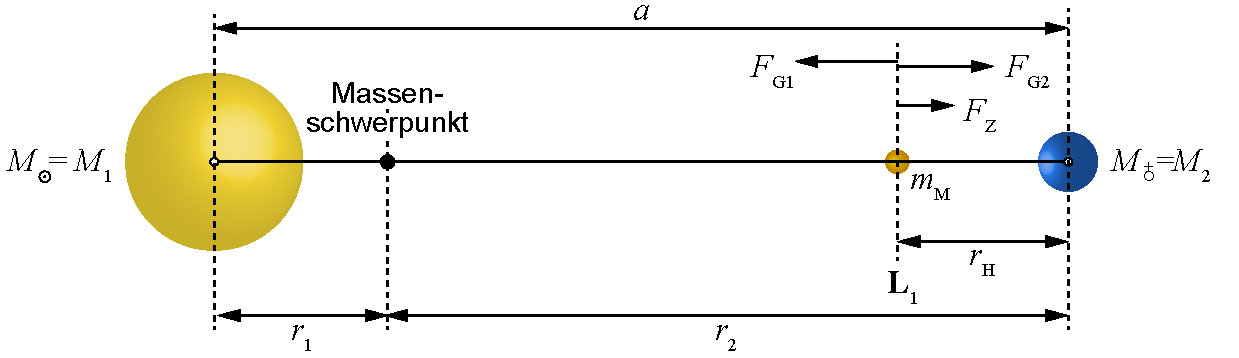
\includegraphics[width=0.8\textwidth]{Moon_of_Moon.pdf} 
	\caption[Zur Ableitung der Stabilit�tsbedingung.]{Zur Ableitung der Stabilit�tsbedingung (Hill Sph�re).}
	\label{abb:hm_Moon_of_Moon}
\end{figure}

Dann wollen wir uns einen ausgezeichneten Punkt zwischen den Massen $m_1$ und $m_2$ anschauen, an dem sich die Testmasse $m$ stabil aufhalten kann.
Dieser Punkt wird Lagrange-Punkt L$_1$ genannt.
Eine dort befindliche Testmasse $m$ rotiert um den Massenschwerpunkt des $m_1$-$m_2$-Systems mit der \emph{gleichen} Winkelgeschwindigkeit $\omega$ wie die Masse $m_2$.\footnote{Gewisserma�en \anf{geh�rt} die Testmasse an diesem Punkt weder zu $m_1$ noch zu $m_2$.
Es ist also der Grenzfall.} Wir erhalten aus der Geometrie der \figref{hm_Moon_of_Moon} die Abst�nde zum Massenschwerpunkt
\begin{align}
	r_1 &= \lk \frac{m_2}{m_1 + m_2} \rk a ~~\text{und} ~~~	r_2 = \lk \frac{m_1}{m_1 + m_2} \rk a ~.\label{eq:hm_moon_moon_lsg2}
\end{align}
Auf die Masse $m$ wirkt wegen ihrer kreisf�rmigen Bewegung um den Massenschwerpunkt die Zentrifugalkraft
\begin{equation}
F_z = m\omega^2 (r_2-r_\text{H}) ~~,\label{eq:hm_moon_moon_lsg3}
\end{equation}
worin wir $\omega$ durch das 3. Keplersche Gesetz ausdr�cken k�nnen:
\begin{equation}
\omega^2 = \frac{G(m_1+m_2)}{a^3}\label{eq:hm_moon_moon_lsg4} ~~.
\end{equation}
Es muss aber auch an dem Punkt L$_1$ die Zentrifugalkraft gleich den wirkenden Gravitationskr�ften der Massen $m_1$ und $m_2$ sein (damit ein Gleichgewicht herrscht), also
\begin{equation}
m\omega^2(r_2 - r_\text{H}) = \frac{Gmm_1}{(a-r_\text{H})^2} - \frac{Gmm_2}{r_\text{H}^2} ~~. \label{eq:hm_eq:moon_moon_lsg5}
\end{equation}
Wir setzen $\omega^2$ aus \eqref{eq:hm_moon_moon_lsg4} ein, dividieren durch $m$ und $G$ und erhalten
\begin{equation}
\frac{m_1+m_2}{a^3}(r_2-r_\text{H}) = \frac{m_1}{(a-r_\text{H})^2} - \frac{m_2}{r_\text{H}^2} ~~.\label{eq:hm_moon_moon_lsg6}
\end{equation}
Mit Substitution von $r_2$, $\gamma_\text{R}\!=\!m_2/m_1$ und $q\!=\!r_\text{H}/a$ erhalten wir aus \eqref{eq:hm_moon_moon_lsg6}
\begin{align}
	m_1 a- (m_1 + m_2) r_\text{H} &= \frac{m_1 a^3}{(a-r_\text{H})^2} - \frac{m_2 a^3}{r_\text{H}^2} ~~\Rightarrow~~a-(1+\gamma_\text{R})r_\text{H} = \frac{a^3}{(a-r_\text{H})^2} - \frac{\gamma_\text{R}a^3}{r_\text{H}^2} \nonumber\\
	\Rightarrow 1-(1+\gamma_\text{R})q &= \frac{1}{(1-q)^2} - \frac{\gamma_\text{R}}{q^2} ~~.\label{eq:hm_moon_moon_lsg7}
\end{align}
Diese Gleichung kann man nur numerisch l�sen, da sie ein Polynom 5. Grades in $q$ ist.
Umgeformt lautet sie
\begin{equation}
(1-q)^2 q^2 - (1+\gamma_\text{R})q^3 (1-q)^2 = q^2 - \gamma_\text{R}(1-q)^2 ~~.\label{eq:hm_moon_moon_lsg8}
\end{equation}
Wir k�nnen die Gleichung entweder numerisch l�sen und erhalten $q\!=\!r_\text{H}/a\!=\!f(\gamma_\text{R})$ (gute �bung in \matlab), oder wir machen eine sinnvolle N�herung, die z.\,B. f�r das Sonne-Erde-Mond-System gilt, mit 
\begin{align*}
	\gamma_\text{R} &= \frac{m_2}{m_1} \ll 1 ,\, q \ll 1 ~~~\Rightarrow 1+\gamma_\text{R} \approx 1 \;,~~(1-q)^2 \approx 1-2q \;~~\frac{1}{(1-q)^2} \approx= 1+2q ~~.
\end{align*}
Dann folgt aus \eqref{eq:hm_moon_moon_lsg7}
\begin{align*}
	1-q &= 1+2q - \frac{\gamma_\text{R}}{q^2} 	\Rightarrow q^2 - q^3 = q^2 + 2q^3 - \gamma_\text{R} ~~~	\Rightarrow ~~3q^3 = \gamma_\text{R} ~~
\end{align*}
und nach Resubstitution von $\gamma_\text{R}$ schlie�lich
\begin{equation}
r_\text{H} = a \sqrt[3]{\frac{m_2}{3 m_1}} ~~.\label{eq:hm_moon_moon_lsg9}
\end{equation}
Damit haben wir den maximalen Radius bestimmt, den ein Satellit mit Masse $m_2$ eines Planeten haben kann, bevor er vollst�ndig in das Gravitationsfeld des Zentralk�rpers mit Masse $m_1$ gelangt und selbst zum Kometen oder Planeten wird.
Dieser Radius wird zu Ehren von G. W. Hill\footnote{George William Hill (1838--1914) war ein US-amerikanischer Mathematiker und Astronom, der besonders auf dem Gebiet der theoretischen Astronomie zu Dreik�rperproblemen und der Mondtheorie forschte.} \emph{Hill-Radius} bzw. das entsprechende Volumen \emph{Hill-Sph�re} genannt.\\
Wir wollen zun�chst $r_\text{H}$ des Sonne-Erde-Mond-Systems berechnen.
Mit den Werten f�r $m_\text{\astrosun}\!=\!1.989\cdot 10^{30}\:$kg und $m_\text{\earth}\!=\!5.972\cdot 10^{24}\:$kg ergibt sich $r_\text{H,\earth}\!\approx\! 1.49\cdot 10^6\:$km.
Der Mond befindet sich mit einem Erdabstand von ca. $383000\:$km also gut innerhalb der Hill-Sph�re. \\
Wie sieht es nun aber beim Erde-Mond-\anf{Mond-Mond}-System aus?
Es folgt mit den Werten $m_\text{\earth}$ und $m_\text{M}\!=\!7.3\cdot 10^{22}\:$ kg ein Radius von $r_\text{H,M}\!\approx\! 61000\:$ km f�r die Hill-Sph�re.
Das ist etwas mehr als $1/7$ der Erde-Mond-Entfernung.
Es k�nnte also durchaus m�glich sein, dass der Mond selbst einen Begleiter hat (oder hatte).
Dass dies aber heute in der Realit�t nicht so ist, liegt an den starken Gezeitenkr�ften, die von Erde und Mond auf den Satelliten wirken und ihn mit der Zeit abbremsen w�rden (siehe \kap{adyn_forces}).
Nach einer gewissen Zeit in der Mondumlaufbahn w�rde die Testmasse (der Satellit) auf den Mond st�rzen. 
Es sei zum Schluss noch erw�hnt, dass die Formel f�r die Hill-Sph�re f�r elliptische Bahnen
\begin{equation}
r_\text{H} = (1-e)\,a\,\sqrt[3]{\frac{m_2}{3m_1}} \,. \label{eq:hm_hill_sphere_allg}
\end{equation}
lautet, was relativ einsichtig ist und im Detail in \cite{Murray2008} nachvollzogen werden kann.
\medskip \end{sol}
\textcolor{blue} {$\rightarrow$ zur} \probref{hm_hill_sphere}.\\
\noindent\rule[1ex]{\textwidth}{0.5pt} \newpage

%-----------------------------------------------------------------------------------------------------------

\begin{sol}{prob:hm_potential_merkur}\label{lsg:hm_potential_merkur} %�bung43
\textbf{Berechnung St�rpotential Merkur}\\
\begin{figure}[H]
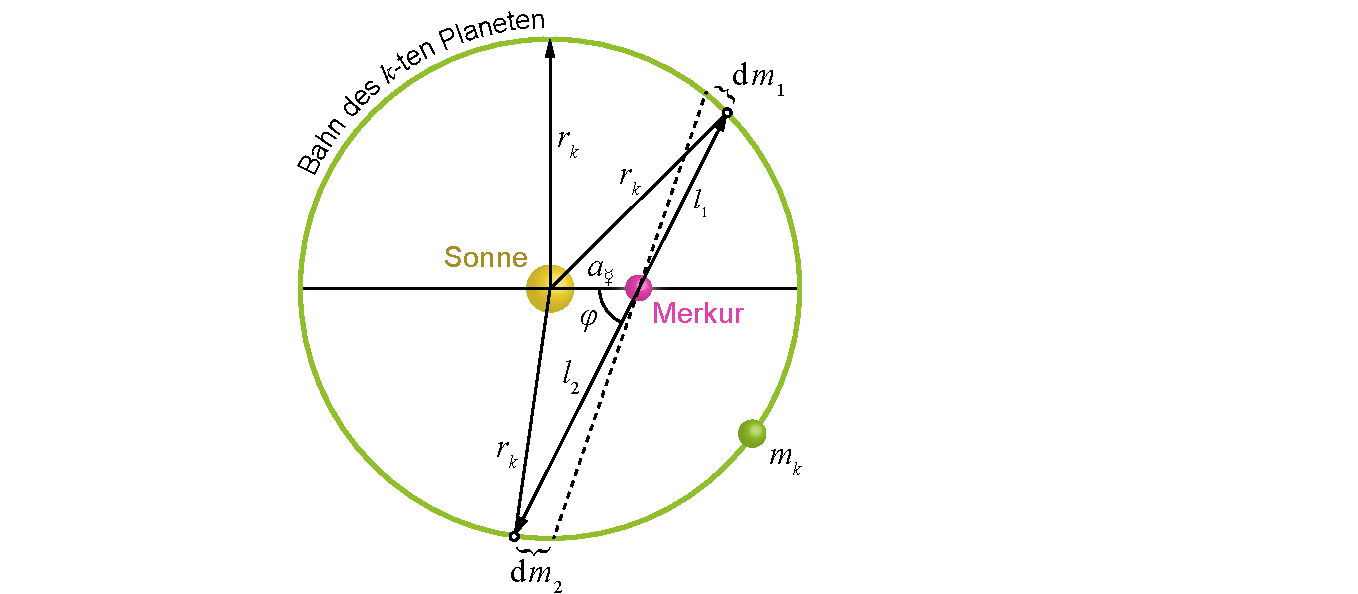
\includegraphics[width=\textwidth]{StoerpotentialMerkur_lsg}%
\caption[Geometrie zur Wirkung des St�rpotentials auf Merkur.]{Geometrie zur Wirkung des St�rpotentials einer Masse $m_k$ auf den Merkur.}%
\label{abb:hm_stoerpot_merkur_lsg}%
\end{figure}

Die Rechnungen sind im Detail im \mscr{} \mlhmref{StoerpotentialMerkur.m} ausgef�hrt. 
\begin{enumerate}[(a)]
	\item Wir benutzen die Geometrie der \figref{hm_stoerpot_merkur_lsg}.
          Der �u�ere Planet mit der Masse $m_k$ bewege sich gleichf�rmig auf der Kreisbahn mit $r_k$.
          Wir k�nnen dann seine Masse im Mittel \anf{verschmiert} auf den Ring mit dem Umfang $2\pi r_k$ verteilt annehmen.
          Die differentielle Massendichte auf der Umlaufbahn des $i$-ten Planeten mit dem Umfang $u_i$, die vom Merkur unter einem Winkel $\varphi$ gesehen wird, ist 
\begin{equation}
\D m_i = \lambda_k \,\D u_i = \frac{m_k}{2\pi r_k}\, l_i\,\D\varphi ~~. \label{eq:hm_pot_merk_lsg1}
\end{equation}
Die Newtonsche Gravitationskraft, die auf den Merkur wirkt, ist jeweils die Differenz der Massenwirkung $\D m_1$ und $\D m_2$, also
\begin{equation}
\D \vec{F} = m_\text{\mercury} G \lk \frac{\D m_1}{l_1^2} - \frac{\D m_2}{l_2^2} \rk \vec{l} ~~. \label{eq:hm_pot_merk_lsg2}
\end{equation}
Hierin ist $\vec{l}$ der Vektor, der vom Merkur zum differentiellen Massepunkt $\D m_1$ zeigt und, wie wir gleich sehen werden, eine Funktion des Winkels $\varphi$ ist.
Die Kraft, die in Richtung der Achse Sonne-Merkur wirkt (das ist die interessante Komponente, die ja das ZK-Feld der Sonne modifiziert), k�nnen wir schreiben als
\begin{equation*}
\D\vec{F}_{\text{SM}} = \D \vec{F}\,\cos\varphi ~~.
\end{equation*}
Wir k�nnen nun �ber $\D\vec{F}_{\text{SM}}$ integrieren und erhalten f�r den Beitrag des $k$-ten �u�eren Planeten �ber
\begin{equation*}
\D\vec{F}_{k,\text{SM}} = \vec{e}_{\text{\astrosun\mercury}}\,\int\limits_{-\pi/2}^{\pi/2} m_\text{\mercury} G \lambda_k \lk \frac{l_2 - l_1}{l_1 l_2} \rk \cos\varphi\,\D\varphi ~~.
\end{equation*}
Hierin haben wir mit $\vec{e}_{\text{\astrosun\mercury}}$ den Einheitsvektor in Richtung Sonne-Merkur bezeichnet.
Wir brauchen jetzt noch die $\varphi$-Abh�ngigkeit der L�ngen $l_1$ und $l_2$.
Mit dem Kosinussatz gilt
\begin{align*}
r_k^2 &= a^2 + l_1^2 - 2a l_1 \cos(\pi-\varphi) \\
\Rightarrow l_1 &= -a \cos\varphi + \sqrt{a^2\cos^2\varphi - \lk a^2-r_k^2 \rk}
\end{align*}
und
\begin{align*}
r_k^2 &= a^2 + l_2^2 - 2a l_2 \cos(\varphi) \\
\Rightarrow l_2 &= a \cos\varphi + \sqrt{a^2\cos^2\varphi - \lk a^2-r_k^2 \rk} ~~.
\end{align*}
Aus \eqref{eq:hm_pot_merk_lsg1} in \eqref{eq:hm_pot_merk_lsg2} eingesetzt erhalten wir
\begin{align*}
\D\vec{F}_{k,\text{SM}} &= m_\text{\mercury} G \lambda_k \lk \frac{l_1}{l_1^2} - \frac{l_2}{l_2^2} \rk \vec{l}\,\D\varphi \\
&= m_\text{\mercury} G \lambda_k \lk \frac{l_2 - l_1}{l_1 l_2} \rk \vec{l}\,\D\varphi ~~.
\end{align*}
Wir erkennen ferner aus der \figref{hm_stoerpot_merkur_lsg}, dass es zu den Kraftkomponenten, die senkrecht zu der Achse Sonne-Merkur wirken, jeweils eine positive und negative Komponente gibt.
Es verbleibt demnach als Netto-Effekt nur eine Komponente des Kraftvektors in Richtung Sonne-Merkur.
Wir machen weiter mit der hilfreichen Beziehung
\begin{align*}
\frac{l_2-l_1}{l_1 l_2} &= \frac{2a_\text{\mercury} \cos\varphi}{\killA{-a^2\cos^2\varphi} + \killA{a^2\cos^2\varphi} - (a^2_\text{\mercury} - r_k^2)} = \frac{2a_\text{\mercury} \cos\varphi}{r_k^2 - a_\text{\mercury}^2}
\end{align*}
und erhalten f�r die Gravitationskraft schlie�lich
\begin{align*}
F_k &= \frac{2 m_\text{\mercury} a_\text{\mercury} G}{r_k^2 - a_\text{\mercury}^2}\,\lambda_k \int\limits_{-\pi/2}^{\pi/2} \cos^2\varphi \, \D\varphi = \frac{\pi m_\text{\mercury} a_\text{\mercury} G \lambda_k}{r_k^2 - a_\text{\mercury}^2} ~~.         
\end{align*}
Die Wirkung des �u�eren Planeten ist also eine zentrale von der Sonne wegziehende Kraft (was nicht ganz �berraschend ist).
Grundlage f�r dieses Ergebnis waren folgende Annahmen:
\begin{itemize}
	\item Konzentrische Kreisbahnen der �u�eren Planeten und des Merkurs um die Sonne
	\item Wirkung des �u�eren Planeten auf den Merkur sind sehr klein
\end{itemize}

\item Wir berechnen die Frequenz $\omega\!=\!\sqrt{(-3/a) b(a)\!-\! b'(a)}\!\equiv\!\sqrt{\beta}$ nach \eqref{eq:hm_lsg_Stoer}.
  Stabile Bahnen gibt es, wenn der Ausdruck $\beta$ unter der Wurzel $>\!0$ ist.
  Wir berechnen die Beschleunigungen aus
\begin{align*}
b(r) &= -\frac{\d}{\d r}\,U(r) ~~\; \text{und} ~~\; b'(r) = -\frac{\d^2}{\d r^2}\,U(r) ~~.
\end{align*}
\begin{itemize}
	\item F�r den Fall $U(r)\!=\!-r^q$ ergibt sich 
	\begin{align*}
		b(r) &= +q r^q ~\;\text{und} ~\;	b'(r)= q(q-1)r^{q-1} ~~.
	\end{align*}
Mit $r\!=\!q\!=\!1$ folgt 
  \begin{align*}
		\beta &= -3q-q(q-1) > 0 ~~, \\
		\beta &= q(q+2) < 0 ~~.
	\end{align*}
Damit ist der stabile Bereich gegeben durch $-2\!<\!q\!<\!0$.
\smallskip
	\item F�r den Fall $U(r)\!=\! -1/r + C/r^3$ ergibt sich 
 	\begin{align*}
		b(r) &= -\frac{1}{r^2} + \frac{3C}{r^4} ~\;\text{und} ~\;	b'(r) = +\frac{2}{r^3} - \frac{12C}{r^5} ~~.
	\end{align*}
Mit $r\!=\!q\!=\!1$ folgt 
   \begin{align*}
		\beta &= -3(-1+3C)-2-12C >0 ~~, \\
		\beta &= 1+3C >0 ~~.
	\end{align*}
Damit ist der stabile Bereich gegeben durch $C\!>\! -1/3$.
\smallskip
\end{itemize}
\end{enumerate}
\medskip \end{sol}
\textcolor{blue} {$\rightarrow$ zur} \probref{hm_potential_merkur}.\\
\noindent\rule[1ex]{\textwidth}{0.5pt} \newpage


%-----------------------------------------------------------------------------------------------------------

\begin{sol}{prob:hm_perihel_kappa3}\label{lsg:hm_perihel_kappa3} %�bung44
\textbf{L�sung der Bewegungsgleichung und Periheldrehung bei einem $\kappa_3/r^3$ St�rpotential und Berechnung der relativistischen Perihelverschiebung des Merkurs}\\ \\
Wir setzen zun�chst in Gleichung \eqref{eq:hm_allg_ZK_1} $\kappa_2\!=\!0$.
Das ergibt
\begin{align}
\D \upsilon &= -\frac{\D q}{\sqrt{\frac{2H_g}{L^2} + \frac{2\mu_\text{G}}{L^2} q - \lk 1 - \frac{2\kappa_3 }{L^2} q \rk q^2 }} \nonumber \\
&= -\frac{\D q}{\sqrt{\hat{A}+ \hat{B} q + \hat{C} q^2 + \hat{D} q^3 }} ~~, \label{eq:hm_perihel_lsg_1} 
\end{align}
mit den Abk�rzungen
\begin{align*}
	\hat{A} = \frac{2H}{L^2} < 0 ~, \: \hat{B} = \frac{2\mu_\text{G}}{L^2} > 0 ~,\:	\hat{C} = -1 < 0 ~\; \text{und} ~\;\hat{D} = \frac{2\kappa_3}{L^2}~~.
\end{align*}
Dieses Integral ist nicht analytisch l�sbar.
Allenfalls kann man eine Reihenentwicklung machen.
Wir verfolgen hier einen st�rungstheoretischen Ansatz \cite{Greiner2003, Stephani1991}.
Dazu schreiben wir wieder die Radialbeschleunigung \eqref{eq:hm_beschl_polar} in Polarkoordinaten:
\begin{equation}
b(r) = b \lk \frac{1}{q} \rk = \lk \ddot{r} - r\dot{\upsilon}^2 \rk = -\frac{\d}{\d r}U(r) ~~.\label{eq:hm_perihel_lsg_2}
\end{equation}
F�r $\dot{r}$ gilt:
\begin{equation*}
\dot{r} = \frac{\D r}{\D \upsilon}\,\dot{\upsilon} = -\frac{1}{\killA{q^2}} \frac{\D q}{\D \upsilon} L \killA{q^2} = -L\,\frac{\D q}{\D \upsilon}~~
\end{equation*}
und analog f�r $\ddot{r}$: 
\begin{align*}
	\ddot{r} = \frac{\D}{\D t}\dot{r} &= -L \, \frac{\D}{\D t} \lk \frac{\D q}{\D \upsilon} \rk = -L \frac{\D }{\D \upsilon}\frac{\D \upsilon}{\D t} \lk \frac{\D q}{\D \upsilon} \rk = -L^2 q^2\,\frac{\D^2 q}{\D \upsilon^2}~~.
\end{align*}
Wir setzen beide Beziehungen in \eqref{eq:hm_perihel_lsg_2} ein und bekommen
\begin{align}
	-L^2 q^2 \,\frac{\D^2 q}{\D \upsilon^2} - \frac{1}{q}\,L^2 q^4 &= -\frac{\d}{\d r}U(r) = -\frac{\mu_\text{G}}{r^2} + \frac{3\kappa_3}{r^4}\nonumber\\
\Rightarrow \frac{\D^2 q}{\D \upsilon^2} + q &= \frac{1}{L^2 q^2}\,\frac{\d}{\d r}U(r) ~\nonumber\\
&= \frac{\mu_\text{G}}{L^2} - \frac{3\kappa_3}{L^2} q^2 ~. \label{eq:hm_perihel_lsg_3} 
 \end{align}
F�r $\kappa_3\!=\!0$ ergibt sich die bemerkenswert einfache Differentialgleichung 
\begin{equation}
\frac{\D^2 q}{\D \upsilon^2} + q = \frac{\mu_\text{G}}{L^2} \label{eq:hm_perihel_lsg_4} ~~, 
\end{equation}
aus deren L�sung sich sehr einfach die Bahnform bestimmen l�sst.
Denn es ist 
\begin{equation}
q(\upsilon) = \frac{\mu_\text{G}}{L^2} + A \cos\upsilon+ B\sin\upsilon \label{eq:hm_perihel_lsg_5} ~~,
\end{equation}
woraus man mit $q\!=\!1/r$ und $A\cos\upsilon + B\sin\upsilon\!=\! C\cos(\upsilon-\upsilon_0)$ nicht �berraschend die bekannte Kegelschnittgleichung \eqref{eq:hm_kegelschnitt} des Keplerproblems erh�lt.\footnote{Ohne Beschr�nkung der Allgemeinheit kann man $\upsilon_0\!=\!0$ setzen.} Wir erweitern nun \eqref{eq:hm_perihel_lsg_5} um $-3\kappa_3 q^2$ und schreiben f�r $\D^2 q / \D \upsilon^2 \!=\! q''$, so dass aus \eqref{eq:hm_perihel_lsg_3} folgt
\begin{align}
	q'' + q &= \frac{\mu_\text{G}}{L^2} - \frac{3\kappa_3 q^2}{L^2} \label{eq:hm_perihel_lsg_6}\\
	&\equiv A + \frac{B}{A}\,q^2 ~~, \nonumber
\end{align}
wobei $A\!=\!\mu_\text{G}/L^2 = 1/p$, $B/A\!=\!-3\kappa_3/L^2$ und $B\!=\!-3\kappa_3\mu_\text{G}/L^4$ gesetzt wurde.
Da $\kappa_3$ und daher $B/A$ kleine Gr��en sind, k�nnen wir f�r die L�sung dieser inhomogenen Differentialgleichung folgenden Ansatz machen:
\begin{align}
q &\approx q_K + B\:\hat{q} ~\label{eq:hm_perihel_lsg_7}\\
\Rightarrow q''_K + q_K + B \hat{q}'' + B\hat{q} &= A + \frac{B}{A} \lk q^2_K + 2 B\! q_K \!\hat{q} + B^2 \hat{q}^2 \rk ~~,
\end{align}
worin $q_K$ die Keplerl�sung f�r $\kappa_3\!=\!0$ ist.
Wir sortieren nach Potenzen von $B$ und bis zur Ordnung mit $B^1$.
Damit ergibt sich
\begin{align}
B^0 : ~ &q''_K + q_K = A ~~. \label{eq:hm_perihel_lsg_8a} \\ 
B^1 : ~ &\hat{q}'' + \hat{q} = \frac{1}{A} \lk q_K^2 + 2B \!q_K \hat{q}\rk = \frac{q_K}{A} \lk q_K + 2\hat{q} B \rk ~~\Rightarrow ~~\hat{q}'' + \hat{q} \lk 1 - \frac{2 B q_K}{A} \rk \approx \frac{q_K^2}{A}~~.  \label{eq:hm_perihel_lsg_8b}
\end{align}
Gleichung \eqref{eq:hm_perihel_lsg_8a} ist wie erwartet die bekannte Kepler-L�sung.
Wir setzen jetzt in \eqref{eq:hm_perihel_lsg_8b} f�r $q_K$ die Bahngleichung in der Form \eqref{eq:hm_kegelschnitt} ein und erhalten mit $q_K(\upsilon) = 1/p (1 + e\cos\upsilon) = A (1 + e\cos\upsilon) $ und $(A=1/p)$
\begin{align*}
	\hat{q}'' + \hat{q} &= p \lek \frac{1}{p} \lk 1+e\cos\upsilon\rk\rek^2 = \frac{1}{p} \lk  1+2e\cos\upsilon + \underbrace{e^2\cos^2\upsilon}_{= \frac{e^2}{2}(1+\cos 2\upsilon)}\rk \\
											&= \frac{1}{p} \lk  1+\frac{e^2}{2}+ 2e\cos\upsilon + \frac{e^2}{2}\cos 2\upsilon \rk~~.
\end{align*}
Da wir an Irregularit�ten der Bahn interessiert sind, schreiben wir die gesuchte Gesamtl�sung als lineare Superposition  $\hat{q}\!=\!\hat{q}_1 + \hat{q}_2 + \hat{q}_3$ und sortieren die einzelnen Elemente nach Vielfachen von $\upsilon$ im Argument des Kosinus:  
\begin{align}
\begin{split}
	\cos(0\upsilon): ~~ \hat{q}''_1 + \hat{q}_1 &= \frac{1}{p} \lk 1+\frac{e^2}{2}\rk~~, \\
	\cos(1\upsilon): ~~ \hat{q}''_2 + \hat{q}_2 &= 2\frac{e}{p} \cos\upsilon ~~, \\
	\cos(2\upsilon): ~~ \hat{q}''_3 + \hat{q}_3 &= \frac{e^2}{2p} \cos 2\upsilon ~~.
\end{split} \label{eq:hm_perihel_lsg_09a}
\end{align}
Die Einzell�sungen $\hat{q}_i$ der linearen Superposition sind (wie man leicht durch Differenzieren verifiziert):
\begin{align}
\begin{split}
\hat{q}_1 &= \frac{1}{p} \lk 1+\frac{e^2}{2}\rk ~~, \\
\hat{q}_2 &= \frac{e}{p}\,\upsilon \sin\upsilon ~~,\\ 
\hat{q}_3 &= -\frac{e^2}{6p}\,\cos 2\upsilon ~~.
\end{split} \label{eq:hm_perihel_lsg_09b}
\end{align}
Der eigentlich interessante Term ist der f�r $\hat{q}_2$.
Man erkennt an dieser Stelle, dass die Periheldrehung durch den nichtlinearen St�ranteil, der in der \eqref{eq:hm_perihel_lsg_3} vorhanden ist, hervorgerufen wird.
Die Gleichung f�r die gest�rte Bahn k�nnen wir schreiben als Keplerbahn plus St�rung $\hat{q}$:
\begin{equation}
q(\upsilon) = q_K + B \hat{q} = \frac{1+e\cos\upsilon}{p} + B (\hat{q}_1 + \hat{q}_2 + \hat{q}_3)~~. \label{eq:hm_perihel_lsg_9}
\end{equation}
Wir wollen jetzt analysieren, wie diese einzelnen St�rungen wirken.
Dazu fahren wir fort mit
\begin{equation}
pq(\upsilon) = 1 + \underbrace{e\cos\upsilon + Be\upsilon\sin\upsilon}_{\text{Term P}} + 1 + B \lek \lk 1+\frac{e^2}{2}\rk - \frac{e^2}{6} \cos{2\upsilon} \rek ~~, \label{eq:hm_perihel_lsg_10}
\end{equation}
wobei nur Term P zur Modifikation der Keplerbahn in Form einer Perihelverschiebung beitragen kann.
Wir k�nnen jetzt mit den Winkelfunktionen und unter Beachtung von $B \ll 1$ folgende Beziehung nutzen:
\begin{align*}
e\cos(\upsilon-B\upsilon)	&= e\cos\upsilon\,\underbrace{\cos(B\upsilon)}_{\approx 1} + e\sin\upsilon\,\underbrace{\sin(B\upsilon)}_{B\upsilon} = e\cos\upsilon + (Be\upsilon)\,\sin\upsilon\,
\end{align*}
Damit vereinfacht sich \eqref{eq:hm_perihel_lsg_10} zu
\begin{align*}
p\,q(\upsilon) &= 1 + \underbrace{e\cos(\upsilon-B\upsilon)}_{\text{Term I}} + B \underbrace{\lk a+\frac{e^2}{2} - \frac{e^2}{6}\,\cos 2\upsilon\rk}_{\text{Term II}}~~,
\end{align*}
wobei Term I \emph{nicht-periodisch} in $2\pi$ ist (und damit zu einer Periheldrehung f�hrt) w�hrend Term II periodisch in $2\pi$ (und damit nur f�r eine Oszillation des Radius verantwortlich ist).
Wir erhalten schlie�lich 
\begin{align}
r(\upsilon)	 &= \frac{p}{1+e\cos(\upsilon-B\upsilon)} \lk 1+ \frac{B C p}{1+e\cos{(\upsilon-B\upsilon)}} \rk^{-1} ~~. \label{eq:hm_perihel_lsg_11}
\end{align}
Damit haben wir eine n�herungsweise Beschreibung der Bahn f�r den gest�rten Fall mit $\kappa_3 \neq 0$ gewonnen.
\begin{figure}[H]
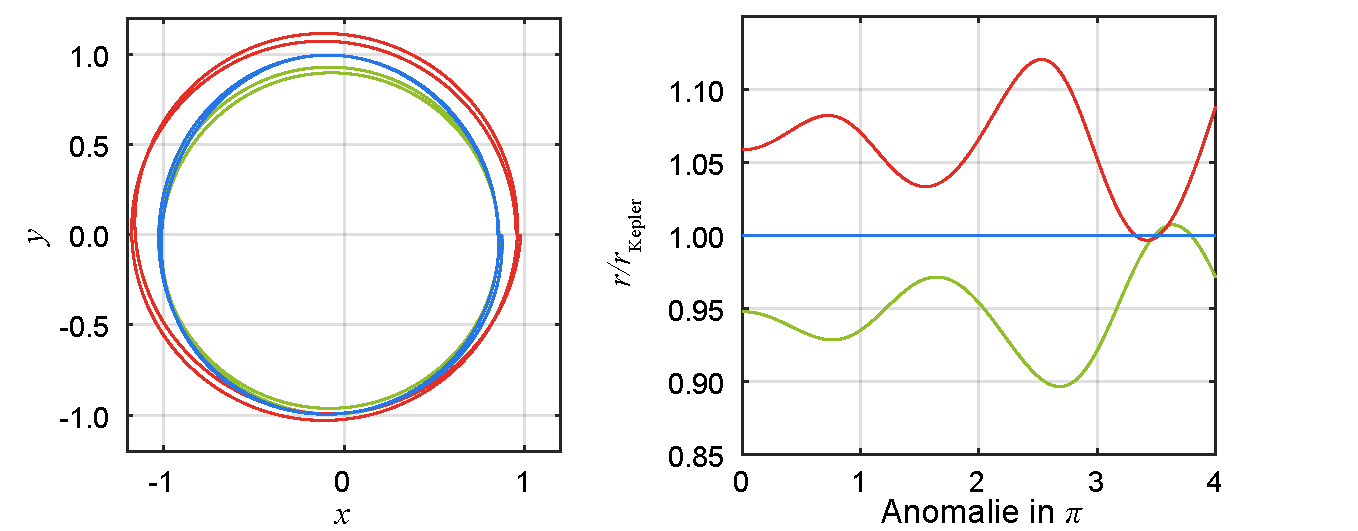
\includegraphics[width=\textwidth]{simulation_merkur2.pdf}%
\caption[Bahnkurven und Bahn-Oszillationen im Fall eines St�rpotentials.]{Bahnkurven und Bahn-Oszillationen im Fall eines St�rpotentials mit $\kappa_3 /{r^3}$\\ Parameter: $a=1, e = 0.1, \kappa_3 = + 0.02\,\mu_\text{G}/a^2 >0 $ (rot) und $\kappa_3-0.02\,\mu_\text{G}/a^2 < 0$ (gr�n). In blauer Farbe ist die Keplerl�sung dargestellt (\scref{prob:hm_perihel_kappa3}).}%
\label{abb:hm_simulationen_merkur2}%
\end{figure} 

F�r $\kappa_3$ k�nnen wir z.\,B. auch das relativistische Zusatzpotential \eqref{eq:hm_einstein_01} einsetzen.
In \figref{hm_simulationen_merkur2} sind im linken Bild die Bahnkurven f�r den Keplerfall (blau) als auch f�r die St�rpotentiale $\kappa_3 = + 0.02 \: \mu_\text{G}/a^2 > 0 $ (rot) und $\kappa_3-0.02 \: \mu_\text{G}/a^2 < 0$ (gr�n) dargestellt.
Im rechten Bild ist der Bahnradius �ber die Anomalie aufgetragen.
Die Bahnoszillationen sind deutlich zu erkennen.\\
Um die Periheldrehung und Verschiebungsrate f�r den Merkur zu erhalten, k�nnen wir mit $\upsilon_{\text{P}_0} (1-B) = 2 \pi $ fortfahren und schreiben:
\begin{align}
		\Delta \upsilon_{\text{P}_0} &= \upsilon_{\text{P}_0} - 2\pi \approx 2\pi \lk (1+B) - 1\rk  ~\: \text{bzw.} \nonumber \\
	\Delta \dot{\upsilon}_{\text{P}_0} &\approx \frac{2\pi B}{T_{\mercury}} = -2\pi\,\frac{3\kappa_3\mu_\text{G}}{T_{\mercury} \, L^4}
~~ \text{mit} ~ B = -\frac{3\kappa_3\mu_\text{G}}{L^4}~. \label{eq:hm_perihel_lsg_12}
\end{align}
Das hei�t, dass die Periheldrehung im Falle $\Delta U_3 \propto 1/r^3$ wie erwartet vom Drehimpuls und der St�rke der St�rung $\kappa_3$ abh�ngt.
F�r ein negatives $\kappa_3$, d.\,h.\, einem zus�tzlich anziehenden Potential, wie es z.\,B. im Fall des relativistischen Beitrags \eqref{eq:hm_einstein_01} vorliegt, ergibt sich ein Voranschreiten des Perihels ($\Delta \dot{\upsilon}_{\text{P}_0} > 0$) in �bereinstimmung mit unseren Absch�tzungen in \eqref{eq:hm_upsilon_P0}.
Setzen wir die Werte von \eqref{eq:hm_einstein_01} ein, erhalten wir mit den Gr��en 
\begin{align*}
\kappa_3 = - \frac{\mu_{\text{G}} L^2}{c^2} ~ \text{und} ~ L^2 \:=\: a \:\mu_{\text{G}} (1-e^2) 
\end{align*}
eine Verschiebungsrate von
\begin{align*}
\Delta \dot{\upsilon}_{\text{P}_0} = \frac{6 \pi}{c^2} \frac{\mu_{\text{G}}}{a(1-e^2)} \frac{1}{T_{\mercury}} \approx 43''/\text{Jh.}.
\end{align*}
Wir sehen, dass unsere Absch�tzung in \eqref{eq:hm_rel_perihel_val} f�r nahezu kreisf�rmige Bahnen in Kapitel \ref{kap:Stabile_Bahnen} sehr gut war.
Unsere st�rungstheoretische L�sung ber�cksichtigt auch noch die Elliptizit�t der Bahn, welche zu einem $4\,\% $ gr��eren Wert der Perihelverschiebung f�hrt.\\

F�r interessierte Leser sei auf eine sch�ne einfache, da linearisierte, Merkurpr�zessionsberechnung f�r den relativistischen Fall in \cite{Hall2022} verwiesen, die ebenfalls f�r ein nichtrelativistisches $\kappa_3/r^3$ St�rpotential verwendet werden kann.\\
\medskip \end{sol}
\textcolor{blue} {$\rightarrow$ zur} \probref{hm_perihel_kappa3}.\\
\noindent\rule[1ex]{\textwidth}{0.5pt} \newpage

%-----------------------------------------------------------------------------------------------------------

\begin{sol}{prob:hm_MoFi}\label{lsg:hm_MoFi} %�bung45
\textbf{Mond- und Sonnenfinsternisse}\\ \\
Aus den �berlegungen von Kapitel \ref{kap:basics_sofis} ist relativ klar, dass eine totale Mondfinsternis sehr h�ufig vor oder nach einer totalen Sonnenfinsternis auftreten muss.
Wir haben die Tage, an welchen im Zeitraum von 1990 bis 2040 m�gliche Sonnenfinsternisse (unabh�ngig vom Ort auf der Erde) und Mondfinsternisse aufgetreten sind \bzw noch auftreten werden, im Detail in \mlhmref{Sonnenfinsternis01.m} ausgef�hrt.
Aus den Rechnungen sieht man, dass am 07.\ August 2017 (18:13:01 UT), also ziemlich genau 14 Tage vor der Sonnenfinsternis vom 21.\ August 2017 (um 18:28.44 UT) eine partielle Mondfinsternis auftrat.
Diese war aber wegen der Uhrzeit und der Position des Mondes in Europa nur in der Endphase zu beobachten.\footnote{Um die Zeiten der Verfinsterung auf eine Sekunde genau berechnen zu k�nnen, braucht man Genauigkeiten in der Ephemeridenrechnung von etwa einer Bogensekunde.
Die in den \mscren verwendeten Funktionen \mlhmiref{SonneExakt.m} und \mlhmiref{MondExakt.m} wurden auf Basis von Daten aus \cite{Montenbruck1999, Meeus1998} geschrieben und haben Genauigkeiten von besser als 5 Bogensekunden.} Aus den Abbildungen erkennt man sehr sch�n das Auftreten von Zyklen der Finsternisse, die bereits im Altertum bekannt waren.
Der bekannteste ist der Saroszyklus\index{Saroszyklus}, der dadurch gekennzeichnet ist, dass seine Periode etwa 18.03 Jahre betr�gt und zwei seiner direkt folgenden Finsternisse sich sehr �hneln.
Das liegt daran, dass nach einer ganzen Zahl anomalistischer Monate der Mond sich wieder an demselben Ort auf seiner elliptischen Bahn um die Erde befindet.
Weil die Sarosperiode nur etwa 11 Tage l�nger als 18 ganze Jahre ist, befindet sich auch die Erde ann�hernd wieder am selben Ort der Erdbahn.
Aus diesem Grund wirft der Mond ann�hernd wieder den gleichen Schatten auf die Erde.

\begin{figure}[H]
\begin{minipage}{\textwidth}
\leftfigure{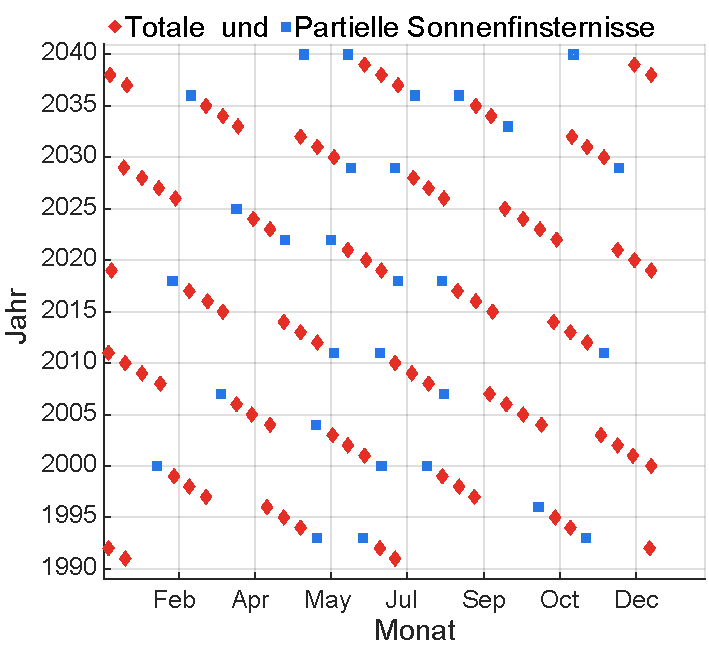
\includegraphics[width=0.5\textwidth]{Sonnenfinsternisse.pdf}}
\hspace{\fill}
\rightfigure{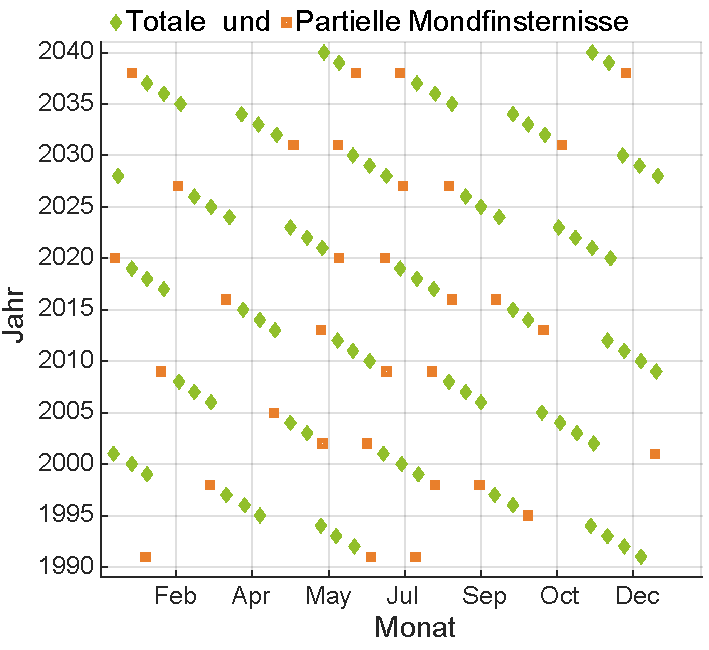
\includegraphics[width=0.5\textwidth]{Mondfinsternisse.pdf}}
\leftcaption[Sonnenfinsternisse 1990--2040.]{Sonnenfinsternisse 1990--2040}\label{abb:hm_Sonnenfinsternisse}
\rightcaption[Mondfinsternisse 1990--2040.]{Mondfinsternisse 1990--2040}\label{abb:hm_Mondfinsternisse}
\end{minipage}
\end{figure}

\medskip \end{sol}
\textcolor{blue} {$\rightarrow$ zur} \probref{hm_MoFi}.\\
\noindent\rule[1ex]{\textwidth}{0.5pt} \newpage

%-----------------------------------------------------------------------------------------------------------



\newpage
\subsection{\mscre--Himmelsmechanik}\label{kap:hm_matlabskripts}

Die \mscre befinden sich im MATLAB-Ordner \texttt{MatlabDateien/hm},
die Hilfsfunktionen im dortigen Unterordner \texttt{Include\-folder} und Daten im Unterordner \texttt{Data}.

Die \mscre befinden sich im MATLAB-Ordner \texttt{MatlabDateien/hm},
die Hilfsfunktionen im dortigen Unterordner \texttt{Include\-folder} und Daten im Unterordner \texttt{Data}.
Es wird empfohlen, entweder die Skripte im GitHub Verzeichnis \githubSN zu benutzen oder sich die komplette Verzeichnisstruktur von \MKc~ runter zu laden und diese und auch das Arbeitsbuch im Hauptverzeichnis Fingeruebungen zu installieren. \\

Wir wollen noch einmal explizit darauf hinweisen, dass die \mscre prim�re der Vermittlung der physikalischen Modelle dienen und keinen Anspruch auf besonders elegante oder effiziente Programmierung erheben. Unser Buch ist ja kein Lehrbuch f�r \matlab-Programmierung. Uns ging es bewusst darum, dass die Skripte gut lesbar sind und das physikalische Modell bzw den physikalischen Gedankengang m�glichst klar abbilden.
Die Leser sind aufgerufen, die Programme nach Belieben zu verbessern und kompakter zu gestalten und diese auch ins GitHub Verzeichnis \githubSN zu stellen.

\subsubsection{Skripte zu Beispielen}\label{mls:hm_bsp_uebungen} %MLSkript1 

\subparagraph{\textbf{Exzentrizit�t Planetenbahnen}}\label{mls:hm_exzentri} %MLSkript2
\begin{longtable}{p{0.33\textwidth}p{0.67\textwidth}}
\hline\noalign{\smallskip}
Skript & Beschreibung \\
\noalign{\smallskip}\svhline\noalign{\smallskip}
\mlhmref{PlanetExzentrizitaeten.m}	& Darstellung der Exzentrizit�ten der Planetenbahnen (auf gro�e Halbachse $a$ normiert).\\
\noalign{\smallskip}\hline\noalign{\smallskip}
\end{longtable}

\subparagraph{\textbf{Analemma}}\label{mls:hm_analemma} %MLSkript3
\begin{longtable}{p{0.33\textwidth}p{0.67\textwidth}}
\hline\noalign{\smallskip}
Skript & Beschreibung \\
\noalign{\smallskip}\svhline\noalign{\smallskip}
\mlhmref{Analemma01.m}        & Analemma auf Basis einer auf der Mittelpunktsgleichung basierenden Keplerl�sung f�r die Sonnenbahn. Exzentrizit�t und Ekliptikschiefe werden variiert (�quinoktium und Ekliptik des Datums). \\
\mlhmref{Analemma02.m}        & Analemmaberechnung (N�herungsrechnung) f�r verschiedene geographische Positionen in Alt-Azimut-Darstellung f�r 24 h. Refraktion und Tagbogenverl�ngerung vernachl�ssigt. Es wird eine einfache auf der Mittelpunktsgleichung basierenden Keplerl�sung f�r die Erdbahn benutzt (�quinoktium und Ekliptik des Datums). \\
\mlhmref{Analemma03.m}        & Analemmaberechnung f�r verschiedene Planeten direkt aus der exzentrischen Anomalie $E$ ohne L�sung der Kepler-Gleichung.\\
\mlhmref{AnalemmaSonne.m}  & Analemmaberechnung der Sonne vom Mond aus auf Basis von auf der Mittelpunktsgleichung basierenden Keplerl�sungen f�r die Sonnen- und Mondbahn.\\
\mlhmref{AnalemmaMond.m}    & Analemmaberechnung f�r Mond von der Erde aus betrachtet auf Basis von auf der Mittelpunktsgleichung basierenden Keplerl�sungen f�r die Sonnen- und Mondbahn.\\
\mlhmref{AnalemmaOkoFit.m}    & Umrechnung einschlie�lich Bildkorrektur des aufgenommenen Analemma von Oberkochen 2019/20 in das horizontale KOS, sowie Darstellung verschiedener theoretisch berechneter Analemma. \\
\mlhmref{AnalemmaFindExz.m}   & Umrechnung einschlie�lich Bildkorrektur des aufgenommenen Analemma von Oberkochen 2019/20 in das horizontale KOS, sowie Fit eines theoretisch berechneten Analemmas mit der Exzentrizit�t e als Parameter. \\
\noalign{\smallskip}\hline\noalign{\smallskip}
\end{longtable}

\subparagraph{\textbf{Sonnenaufgangsberechnung (Methode der quadratischen Interpolation)}}\label{mls:hm_sonnenaufgang} %MLSkript4
\begin{longtable}{p{0.33\textwidth}p{0.67\textwidth}}
\hline\noalign{\smallskip}
Skript & Beschreibung \\
\noalign{\smallskip}\svhline\noalign{\smallskip}
\mlhmref{Sonnenaufgang01.m} & Aufgangs- und Untergangszeiten der Sonne f�r verschiedene geographische Orte (Breite < 60�) und die Tagl�ngen
 iterativ aus der Kepler-Gleichung f�r das ganze Jahr und in der N�he des Jahreswechsels bzw. Mitsommers.\\
\mlhmref{Sonnenaufgang02.m} & Aufgangszeiten auf Basis der Kepler-Gleichung  a) mit einer iterativen Methode (Quadratische 
Interpolation) zur Suche der Nullstellen f�r Auf- und Unterg�nge und b) zum Vergleich auf Basis der ZGL-N�herung.\\
\noalign{\smallskip}\hline\noalign{\smallskip}
\end{longtable}

\subparagraph{\textbf{Vergleich Zeitgleichung}}\label{mls:hm_zeitglgformeln} %MLSkript5
\begin{longtable}{p{0.33\textwidth}p{0.67\textwidth}}
\hline\noalign{\smallskip}
Skript & Beschreibung \\
\noalign{\smallskip}\svhline\noalign{\smallskip}
\mlhmref{ZGL01.m} & ZGL auf Basis einer Mittelpunktsgleichung basierenden Keplerl�sung f�r die Sonnenbahn und Vergleich mit empirischen Werten und den Berechnungen des JPL (�quinoktium und Ekliptik des Datums). \\
\mlhmref{ZGL02.m} & Reihenentwicklung der ZGL.\\
\mlhmref{ZGL03.m} & ZGL auf Basis einer (auf der Mittelpunktsgleichung basierten) Keplerl�sung f�r die Erdbahn und Vergleich mit verschiedenen publizierten N�herungsformeln und den Berechnungen des JPL. \\
\noalign{\smallskip}\hline\noalign{\smallskip}
\end{longtable}
 
\subparagraph{\textbf{Tagbogen-Verl�ngerung}}\label{mls:hm_tagbogenverl} %MLSkript6
\begin{longtable}{p{0.33\textwidth}p{0.67\textwidth}}
\hline\noalign{\smallskip}
Skript & Beschreibung \\
\noalign{\smallskip}\svhline\noalign{\smallskip}
\mlhmref{TagbogenVerlaengerung.m} & Tagbogenverl�ngerung bedingt durch Refraktion und scheinbaren Sonnendurchmesser bei Sonnenaufgang.\\
\noalign{\smallskip}\hline\noalign{\smallskip}
\end{longtable}

%\newpage
\subparagraph{\textbf{Tageslauf Sonne}}\label{mls:hm_tageslauf_sonne} %MLSkript7
\begin{longtable}{p{0.33\textwidth}p{0.67\textwidth}}
\hline\noalign{\smallskip}
Skript & Beschreibung \\
\noalign{\smallskip}\svhline\noalign{\smallskip}
\mlhmref{TageslaufSonne01.m} & Der Tageslauf der Sonne wird nach der N�herungsformel (3.84) berechnet. Die geographische Breite kann variiert werden. Es wird die H�he der Sonne f�r verschieden Jahreszeiten und geographische Breiten dargestellt. Die ZGL wird nicht ber�cksichtigt.
Berechnung des Tagbogenverlaufs (N�herung) der Sonne �ber dem Horizont f�r verschiedene Jahreszeiten und geographische Breiten.\\
\mlhmref{TageslaufSonne02.m} & Tagbogenverlauf der Sonne �ber dem Horizont. (N�herungsformel und zum numerische L�sung. Die geographische Breite kann variiert werden.\\
\noalign{\smallskip}\hline\noalign{\smallskip}
\end{longtable}
 


\subparagraph{\textbf{Berechnung der Aufgangswinkel der Sonne (Verschiedene Orte und Jahreszeiten)}}\label{mls:hm_aufgangswinkel_sonne} %MLSkript8
\begin{longtable}{p{0.33\textwidth}p{0.67\textwidth}}
\hline\noalign{\smallskip}
Skript & Beschreibung \\
\noalign{\smallskip}\svhline\noalign{\smallskip}
\mlhmref{SonnenaufgangZeit.m}    & H�he $h$ und Azimut $\mathcal{A}$ und die Zeit-H�hen-Kurven beim Sonnenaufgang auf Basis einer MPG-Keplerl�sung f�r verschiedene geographische Breiten und verschiedene Jahreszeiten (Wintersonnenwende, Fr�hlingsanfang, Sommersonnenwende, Herbstanfang). Dabei wird die astrometrische H�he $h$ und die durch Refraktion \ua Effekte bedingte \anf{scheinbare} H�he $h'$ berechnet.\\ 
\mlhmref{SonnenaufgangBaabe.m}        & H�he $h$ und Azimut $\mathcal{A}$ und die Zeit-H�hen-Kurven beim Sonnenaufgang auf Basis einer MPG-Keplerl�sung f�r die Erdbahn f�r Baabe (Ostsee). Dabei wird die astrometrische H�he $h$ und die durch Refraktion \ua Effekte bedingte \anf{scheinbare} H�he $h'$ berechnet.\\
\noalign{\smallskip}\hline\noalign{\smallskip}
\end{longtable}
 

\subparagraph{\textbf{Innere Planetenbahnen}}\label{mls:hm_innere_planeten} %MLSkript9
\begin{longtable}{p{0.33\textwidth}p{0.67\textwidth}}
\hline\noalign{\smallskip}
Skript & Beschreibung \\
\noalign{\smallskip}\svhline\noalign{\smallskip}
\mlhmref{InnerePlaneten.m} & Bahnen der inneren Planeten auf Basis der Kepler-Geichung. 
(�quinoktium und Ekliptik des Datums) \\
\mlhmref{VenusTransit01.m} & Koordinaten der Venus und des Merkurs bei Transits. Die Zeiten m�ssen n�herungsweise z.\,B. aus \mlhmref{InnerePlaneten.m} bekannt sein. Die Daten werden mit JPL-Daten verglichen. \\
\mlhmref{VenusTransit02.m} & Bestimmung der Astronomischen Einheit aus den Daten eines Venustransits. a) Parallaxen-Methode nach Halley: Die beobachteten Werte f�r zwei geographische Orte zu einer Zeit UT werden dem Internet entnommen, daraus wird die Parallaxe bestimmt und daraus dann die AE berechnet.  b) Kontaktzeitmethode durch Beobachtung an einem Standort.\\
\noalign{\smallskip}\hline\noalign{\smallskip}
\end{longtable}

\subparagraph{\textbf{�u�ere Planetenbahnen}}\label{mls:hm_aussere_planeten} %MLSkript10
\begin{longtable}{p{0.33\textwidth}p{0.67\textwidth}}
\hline\noalign{\smallskip}
Skript & Beschreibung \\
\noalign{\smallskip}\svhline\noalign{\smallskip}
\mlhmref{AeusserePlaneten.m} & Bahnen der �u�eren Planeten auf Basis der Kepler-Gleichung f�r den Zeitraum 1920--2020. (�quinoktium und Ekliptik des Datums) \\
\noalign{\smallskip}\hline\noalign{\smallskip}
\end{longtable}
 
\subparagraph{\textbf{St�rungsrechnung }}\label{mls:hm_stoerunsgrechnung_planeten} %MLSkript11
\begin{longtable}{p{0.33\textwidth}p{0.67\textwidth}}
\hline\noalign{\smallskip}
Skript & Beschreibung \\
\noalign{\smallskip}\svhline\noalign{\smallskip}
\mlhmiref{VenusExakt.m} & Ekliptikale Koordinaten der Venus auf Basis einer Reihenentwicklung \cite{Montenbruck1999}. \\
\mlhmiref{MarsExakt.m} & Ekliptikale Koordinaten des Mars auf Basis einer Reihenentwicklung \cite{Montenbruck1999}. \\
\mlhmiref{JupiterExakt.m} & Ekliptikale Koordinaten des Jupiters auf Basis einer Reihenentwicklung \cite{Montenbruck1999}. \\
\mlhmiref{SonneExakt.m}  & Ekliptikale Koordinaten der Sonne auf Basis der Newcombschen Theorie \cite{Montenbruck1999}. \\
\mlhmiref{MondExakt.m}. & Geozentrisch-�quatoriale Koordinaten des Mondes auf Basis der Brownschen Theorie \cite{Montenbruck1999}. \\
\mlhmref{SL9numerisch.m} & Bahn des Kometen Shoemaker-Levy 9 bis zu seinem Zusammenprall mit dem Jupiter �ber numerische Integration.
\end{longtable}


\subparagraph{\textbf{Periheldrehung des Merkurs}}\label{mls:hm_perihel_merkur} %MLSkript12
\begin{longtable}{p{0.33\textwidth}p{0.67\textwidth}}
\hline\noalign{\smallskip}
Skript & Beschreibung \\
\noalign{\smallskip}\svhline\noalign{\smallskip}
\mlhmref{PerihelKappa2.m}    & Perihel-Verschiebung f�r ein Potential mit Term $\kappa_2 \neq 0$. \\
\mlhmref{PerihelKappa3.m}    & Perihel-Verschiebung f�r ein Potential mit Term $\kappa_3 \neq 0$. \\
\mlhmref{StoerpotentialMerkur.m}  & St�rpotentiale und Gravitationskr�fte der anderen Planeten auf den Merkur als Ursache der Perihel-Verschiebung des Merkurs nach der Newtonschen Mechanik. \\
\noalign{\smallskip}\hline\noalign{\smallskip}
\end{longtable}

\subparagraph{\textbf{Kometenbahnen}}\label{mls:hm_kometenbahnen} %MLSkript13
\begin{longtable}{p{0.33\textwidth}p{0.67\textwidth}}
\hline\noalign{\smallskip}
Skript & Beschreibung \\
\noalign{\smallskip}\svhline\noalign{\smallskip}
\mlhmref{AsteroidenBahnen.m}   & Bahnen der Asteroiden in heliozentrischen Koordinaten unter Benutzung der Gau�schen Vektoren (�quinoktium und Ekliptik des Datums). \\
\mlhmref{AsteroidenZeit.m}     & Bahn eines Asteroiden als Funktion der Zeit unter fallweiser Benutzung einer parabolischen N�herung. (�quinoktium und Ekliptik des Datums). \\
\mlhmref{KometenBahnen.m}      & Bahnen der Kometen in heliozentrischen Koordinaten unter Benutzung der Gau�schen Vektoren (�quinoktium und Ekliptik des Datums).\\
\mlhmref{KometenZeit.m}        & Bahn eines Kometen als Funktion der Zeit unter fallweiser Benutzung einer parabolischen N�herung (�quinoktium und Ekliptik des Datums). \\
\mlhmref{KometenObsEqu.m}      & Kometenbahnen in Erdn�he als Funktion der Zeit und die Beobachtungsdaten (Rektaszension und Deklination) unter Benutzung von parabolischen N�herungen.\\
\mlhmref{KometenObsHor.m}      & Kometenbahnen in Erdn�he als Funktion der Zeit und die Beobachtungsdaten (Azimut und H�he) unter Benutzung von parabolischen N�herungen.\\
\mlhmref{KometenSL9.m}         & Kepler-Bahn des Kometen D/1993 F2-D (Shoemaker-Levy 9) als Funktion der Zeit und Vergleich mit Werten des JPL \cite{JPL2020} (�quinoktium und Ekliptik des Datums). \\
\mlhmref{KometenHalley.m}      & Bahnen des Kometen Halley von 1986 und 1758 (�quinoktium und Ekliptik Datums). \\
\noalign{\smallskip}\hline\noalign{\smallskip}
\end{longtable}

\subparagraph{\textbf{Gezeiten}}\label{mls:hm_gezeiten} %MLSkript13
\begin{longtable}{p{0.33\textwidth}p{0.67\textwidth}}
\hline\noalign{\smallskip}
Skript & Beschreibung \\
\noalign{\smallskip}\svhline\noalign{\smallskip}
\mlhmref{Gezeitenellipsoid.m}  & Berechnet die Form des Gezeitenellipsoids. \\
\mlhmref{GezeitenReibung01.m}  & Berechnet Parameter der Gezeitenreibung auf der Erde. \\
\mlhmref{GezeitenReibung02.m}  & Berechnet Parameter der Gezeitenreibung auf der Erde mit einem einfachen Hantelmodell.\\
\mlhmref{UmlaufErdeMond.m}     & Simuliert die Bewegung von Erde und Mond um gemeinsamen Schwerpunkt im Laufe eines Monats.\\
%\mlhmref{GezeitenDGLSystem.m}  & L�st das DGLS-System f�r ZKP inklusive Gezeitenreibung.\\
\mlhmref{SimulationAiry.m}     & Simuliert stehende Wellen nach dem Airy-Modell.\\
\noalign{\smallskip}\hline\noalign{\smallskip}
\end{longtable}


\subparagraph{\textbf{Sonnenfinsternisse}} \label{mls:hm_so_fis} %MLSkript14
\medskip
Diese Programme wurden in Teilen auf Basis der C++ Programmstrukturen und der Beschreibung/Erl�uterung in  
"Astronomie mit dem Personal Computer" von Oliver Montenbruck und Thomas Pfleger \cite{Montenbruck1999} entwickelt. 
Genehmigung des Verlages und der Autoren liegt vor.
\begin{longtable}{p{0.33\textwidth}p{0.67\textwidth}}
\hline\noalign{\smallskip}
Skript & Beschreibung \\
\noalign{\smallskip}\svhline\noalign{\smallskip}
\mlhmref{Sonnenfinsternis01.m}    & Zeiten des Neu/Vollmondes in einem bestimmten Zeitraum und bestimmt, ob zu der Neumond/Vollmondzeit eine Sonnen- oder Mondfinsternis stattfinden kann. F�r die Koordinaten Sonne und Mond werden genauere Reihen verwendet. \\
%\mlhmref{PhaseFunc.m} 	& Hilfsfunktion zur Berechnung der Zeiten des Neu/Vollmondes und von Finsternissen.\\
\mlhmref{Sonnenfinsternis02.m}    &  Startet von ungef�hren Neumondzeiten und bestimmt, wann und wo um die Neumondzeit eine Sonnenfinsternis stattfinden kann. F�r die Sonnenfinsternis wird die Zentrallinie der sogenannten maximalen Verfinsterung berechnet.\\
\mlhmref{Sonnenfinsternis03.m}    &  Bestimmt ausgehend vom Neumondzeitpunkt f�r einen gew�hlten Beobachtungsort die Phase, Gr��e und Kontaktzeiten einer Sonnenfinsternis.\\
\noalign{\smallskip}\hline\noalign{\smallskip}
\end{longtable}
 
\subparagraph{\textbf{Lange Zeiten}}\label{mls:hm_lange_zeiten} %MLSkript15
\begin{longtable}{p{0.33\textwidth}p{0.67\textwidth}}
\hline\noalign{\smallskip}
Skript & Beschreibung \\
\noalign{\smallskip}\svhline\noalign{\smallskip}
\mlhmref{ZGL04.m} & Zeitgleichung und Analemma �ber Zeitr�ume von mehreren Jahrtausenden. \\
\noalign{\smallskip}\hline\noalign{\smallskip}
\end{longtable}

\medskip
\subsubsection{Skripte zu verschiedenen �bungen}\label{mls:hm_uebungen} %MLSkript�bungen
\begin{longtable}{p{0.33\textwidth}p{0.67\textwidth}}
\hline\noalign{\smallskip}
Skript & Beschreibung \\
\noalign{\smallskip}\svhline\noalign{\smallskip}
\mlhmref{AbflachungSonne.m}         & Abflachung der Sonne bei Sonnenuntergang als Funktion der H�he.\\
\mlhmref{AnalemmaAnomalie.m}      & Zeitgleichung und Analemma direkt aus der exzentrischen Anomalie.\\
\mlhmref{AufprallgeschwindigkeitKomet.m}        & Aufprallgeschwindigkeit von Kometen/Meteoriten auf der Erde als Funktion verschiedener Parameter.\\
\mlhmref{Besselreihe.m}         & Bessel-Reihe f�r exzentrische Anomalie $E$ f�r verschiedene Exzentrizit�ten $e$ und Summationsgrenzen.\\
\mlhmref{KeplerVergleich.m}         & L�sung der Kepler-Gleichung �ber verschiedene Iterationsverfahren f�r verschiedene Exzentrizit�ten zwischen 0.1, 0.2,.....0.999. Vergleich der Iteration mit Regula falsi und Newton-Raphson f�r verschiedene Anfangswerte der mittleren Anomalie M.\\
\mlhmref{LangzeitJahreszeiten.m}         & Dauer der Jahreszeiten und Energieeintrag der Sonne auf die Nordhemisph�re f�r einen Zeitraum von 8000 Jahren. Einfache Modellierung der Ver�nderungen von Exzentrizit�t, Ekliptikneigung und Richtung der Erdachse.\\
\mlhmref{Mondbahn01.m}         & Mondbahn f�r ein einfaches koplanares ZK-Planet-Mond-System bezogen auf den Zentralk�rper f�r verschiedene Verh�ltnisse der Umlaufzeiten TM (Mond um Planet) und TP (Planet um ZK). \\
\mlhmref{Mondbahn02.m}         & Heliozentrische Mondbahn aus den Ephemeriden.\\
\mlhmref{MarsOpposition.m}         & Marsoppositionen im Zeitraum 2000--2020.\\
\mlhmref{MondErdeSonneApollo8.m}        & Programm berechnet die Positionen von Mond, Erde, Sonne und Apollo 8 am 24.12.1968.\\
\mlhmref{OlympusMons.m}         & Sonnenaufgang auf dem Mars.\\
\mlhmref{PlanetenbahnenKepler.m}         & Bahnen der Planeten Venus bis Jupiter auf Basis der Kepler-Gleichung. Venus-Jupiter-Konjunktion f�r den 22.\ 11.\ 2065 die  (�quinoktium und Ekliptik des Datum). \\
\mlhmref{Refraktion.m}         & Refraktionsberechnung f�r das Kugelschalen-Schichtenmodell und Vergleich mit der Normalrefraktion.\\
\mlhmref{RocheLimit.m}         & Berechnet Roche-Limit und Hill-Sph�ren f�r Planeten unseres Sonnensystems.\\
\mlhmref{SonnenaufgangReinsch.m}         & Analytische Formel f�r Sonnenaufgang nach \cite{Reinsch2003} und Vergleich mit numerischer Berechnung.\\
\mlhmref{SonnenuhrAnalem.m}  & Berechnet Lineatur einer analemmatischen Sonnenuhr f�r G�rlitz.\\
\mlhmref{SimulationAiry.m}  & Simuliert das Airy-Kanal-Modell der dynamischen Theorie der Gezeiten.\\
\mlhmref{TageslaufSonne.m}         & Tageslauf der Sonne mit Ber�cksichtigung der Refraktion $R$ und �ber den Tag ver�nderlicher Deklination $\delta$.\\
\mlhmref{VenusMerkurTransit.m}         & Venustransits am 08.06.2004 und am 06.06.2012.\\
\mlhmref{VerweildauerKomet.m}        & Verweildauer von Kometen in Erdn�he.\\
\mlhmref{Wandsonnenuhr.m}    & Berechnet Lineatur einer Wandsonnenuhr.\\
\mlhmref{ZGLAnalemma.m}      & Zeitgleichung und Analemma auf anderen Planeten (Methode Allison).\\
\mlhmref{ZGLAnalemmaKepler.m}      & Zeitgleichung und Analemma auf anderen Planeten (Methode Montenbruck).\\
\noalign{\smallskip}\hline\noalign{\smallskip}
\end{longtable}

%\newpage
\subsubsection{Hilfsfunktionen}\label{mls:hm_hilfsfunktionen} %MLSkript1 
Einige der Programme wurden in Teilen mit freundlicher Genehmigung der Autoren auf Basis der C++ Programmstrukturen und der Beschreibung/Erl�uterung in \glqq Astronomie mit dem Personal Computer\grqq{} von Oliver Montenbruck und Thomas Pfleger \cite{Montenbruck1999} entwickelt.\\
\begin{longtable}{p{0.33\textwidth}p{0.67\textwidth}}
\hline\noalign{\smallskip}
Skript & Beschreibung \\
\noalign{\smallskip}\svhline\noalign{\smallskip}
Mathematische Funktionen \\
\noalign{\smallskip}\svhline\noalign{\smallskip}
\mlhmiref{CalcAnglesfromXYZ.m}         & Sph�rische Koordinaten aus kartesischen Koordinaten.\\
\mlhmiref{CalcXYZfromAngles.m}         & Kartesische Koordinaten aus sph�rischen Koordinaten.\\
\mlhmiref{Frac.m}                      & Nachkommastellen.\\
\mlhmiref{Modulo.m}                    & Modulus-Funktion.\\
\mlhmiref{R\_x.m}, \mlhmiref{R\_y.m}, \mlhmiref{R\_z.m},     & Rotationsmatrizen bez�glich x,y,z-Achse.\\
\mlhmiref{Stumpff.m}                   & Stumpffsche Funktionen.\\
\noalign{\smallskip}\svhline\noalign{\smallskip}
Hilfsfunktionen f�r Ein- und Ausgabe \\
\noalign{\smallskip}\svhline\noalign{\smallskip}
\mlhmiref{GetColorLines.m}             & L�dt Farbtabelle f�r Linien und graphische Darstellungen.\\
\mlhmiref{StrDMS.m}                    & Umrechnung von Formaten f�r Ausgabe von Winkeln von Dezimal in Grad, Bogenminute, Bogensekunde.\\
\mlhmiref{HMS.m}                       & Umrechnung von Formaten f�r Zeit von Dezimal in hh:mm:ss.s \\
\mlhmiref{StrHMS.m}                    & Umrechnung von Formaten f�r Ausgabe von Zeit von Dezimal in hh:mm:ss.s \\
\mlhmiref{LabelPoints.m}               & Beschriftung von Datenpunkten.\\
\mlhmiref{OrbitParameter.m}            & Einlesen der Bahnparameter der Planeten.\\ 
\mlhmiref{KometParameter.m}            & Einlesen der Bahnparameter der Kometen.\\
\mlhmiref{ImportPlanetParameter.m}     & Einlesen typischer physikalischer Bahnparameter der Planeten und des Mondes.\\

\noalign{\smallskip}\hline\noalign{\smallskip}
Astronomische Funktionen \\
\noalign{\smallskip}\svhline\noalign{\smallskip}
\mlhmiref{Jd.m}                        & Julianisches Datum aus dem Kalenderdatum.\\
\mlhmiref{MJD.m}                       & Modifiziertes Julianisches Datum aus dem Kalenderdatum.\\
\mlhmiref{Jd2JJht.m}                   & Umrechnung von Julianischem Datum in Julianisches Jahrhundert.\\
\mlhmiref{JJht2Jd.m}                   & Umrechnung von Julianischem Jahrhundert in Julianisches Datum.\\
\mlhmiref{GMST.m}                      & GMST (Greenwich Mean Sidereal Time) aus MJD.\\
\mlhmiref{LMST.m}                      & LMST (Local Mean Sidereal Time) aus MJD und geographischer L�nge.\\
\mlhmiref{EpsErde.m}                   & Ekliptikneigung als Funktion der Zeit.\\
\mlhmiref{EAnom.m}                     & Exzentrische Anomalie durch Iteration.\\  
\mlhmiref{Ellip.m}                     & Elliptische Koordinaten aus exzentrischer Anomalie.\\
\mlhmiref{FindRiseSet.m}               & Nullstellensuche Sonnen-Auf- und Untergang im Intervall 0..24 h mit quadratischer Interpolation.\\
\mlhmiref{PQR.m}                       & Multiplikation mit Transformationsmatrix aus Gau�schen Vektoren.\\
\mlhmiref{KometPQR.m}                  & Ekliptikale und �quatoriale Koordinaten von Kometen.\\
\mlhmiref{KometOrbits.m}               & Bahnen der Kometen im Raum.\\
\mlhmiref{PlanetPQR.m}                 & Ekliptikale und �quatoriale Koordinaten von Planeten.\\
\mlhmiref{PlanetOrbits.m}              & Bahnen der Planeten im Raum.\\
\mlhmiref{SonnePQR.m}                  & Ekliptikale und �quatoriale Koordinaten der mittleren Sonne von beliebigen Planeten aus.\\ 
\mlhmiref{KeplerMond.m}                & Mittelpunktsgleichung-L�sung f�r Mond.\\
\mlhmiref{KeplerSonne.m}               & Mittelpunktsgleichung-L�sung f�r Sonne.\\
\mlhmiref{KeplerSonneEx.m}             & Mittelpunktsgleichung-L�sung f�r Sonne -- �quinoktium des Datums und ver�nderliche Exzentrizit�ten.\\
\mlhmiref{KeplerSonneLang.m}           & Mittelpunktsgleichung-L�sung f�r Sonne -- Modellierung f�r gro�e Zeitabst�nde von J2000.\\
%\mlhmiref{SinAlt.m} & Berechnet den Sinus der H�he aus Deklination, Stundenwinkel und Breitengrad.\\ 
\mlhmiref{Convert2Equ.m}               & Umwandlung von ekliptikalen Koordinaten in �quatoriale Koordinaten.\\ 
\mlhmiref{MondExakt.m}                 & Geozentrische Koordinaten des Mondes nach der Brownschen Theorie \cite{Montenbruck1999, Meeus1998}.\\
\mlhmiref{SonneExakt.m}                & Geozentrische Koordinaten der Sonne nach der Newcomschen Theorie \cite{Montenbruck1999, Meeus1998}.\\
\mlhmiref{VenusExakt.m}                & Heliozentrische Koordinaten der Venus nach der St�rungstheorie \cite{Montenbruck1999, Meeus1998}.\\
\mlhmiref{JupiterExakt.m}              & Heliozentrische Koordinaten des Jupiter nach der St�rungstheorie \cite{Montenbruck1999, Meeus1998}.\\
\noalign{\smallskip}\svhline\noalign{\smallskip}
\end{longtable}

\newpage
\subsubsection{Datenfiles} \label{mls:hm_datafiles} %MLSkripteDaten
\begin{longtable}{p{0.4\textwidth}p{0.6\textwidth}}
\hline\noalign{\smallskip}
Skript & Beschreibung \\
\noalign{\smallskip}\svhline\noalign{\smallskip}
csv - Files \\
\noalign{\smallskip}\svhline\noalign{\smallskip}
\mlhmdref{AnalemmaOko2019.csv}              & Analemma-Bilddaten von Aufnahmen in 2019.\\
\mlhmdref{Bahnparameter.csv}                & Bahnparameter f�r �quinoktium und Ekliptik des Datums.\\
\mlhmdref{BahnparameterJ2000.csv}           & Bahnparameter f�r �quinoktium und Ekliptik J2000 \cite{Meeus1998}.\\
\mlhmdref{BahnparameterAbleitung.csv}       & Erste zeitliche Ableitung der Bahnparameter f�r �quinoktium und Ekliptik des Datums.\\
\mlhmdref{BahnparameterJ2000Ableitung.csv}  & Erste zeitliche Ableitung der Bahnparameter f�r �quinoktium und Ekliptik J2000 \cite{Meeus1998}.\\
\mlhmdref{Kometen.csv}                      & Bahnparameter f�r einige ber�hmte Kometen.\\
\mlhmdref{ParaLangzeit.csv}                 & Parameter f�r Langzeitver�nderungen der Bahnparameter der Erde.\\
\mlhmdref{PlanetenFarben.csv}               & Daten f�r Farbkonventionen f�r Planetendarstellungen etc. Wird mit \mlhmiref{GetColorLines.m} eingelesen.\\
\mlhmdref{SL9.csv}                          & Daten f�r Komet Shoemaker-Levy 9 \cite{JPL2020}.\\
\mlhmdref{SonnePos.csv}                     & Parameter f�r St�rungsrechnung der Sonne \cite{Montenbruck1999, Meeus1998}.\\
\mlhmdref{VenusPos.csv} etc.                & Parameter f�r St�rungsrechnung der Planeten \cite{Montenbruck1999, Meeus1998}.\\
\noalign{\smallskip}\svhline\noalign{\smallskip}
dat - Files \\
\noalign{\smallskip}\svhline\noalign{\smallskip}
\mlhmdref{Sonne20040608.dat}         & Koordinaten der Sonne (RA, Deklination) f�r den 08.\,06.\,2004 \cite{JPL2020}.\\
\mlhmdref{Venus20040608.dat}         & Koordinaten der Venus (RA, Deklination) f�r den 08.\,06.\,2004 \cite{JPL2020}.\\
\mlhmdref{ZGLhorizonJPL.dat}         & Daten f�r ZGL 2000 \cite{JPL2020}.\\
\mlhmdref{ZGLempirisch.dat}          & Empirische Daten der ZGL.\\
\noalign{\smallskip}\svhline\noalign{\smallskip}
\end{longtable}



\clearpage
\setcounter{chapter}{4}
\setcounter{section}{3}
\setcounter{subsection}{0}
\setcounter{figure}{0}
\setcounter{equation}{0}
\setcounter{prob}{0}
\counterwithin{table}{section}
\setcounter{table}{0}
\section{L�sungsbeispiele \autoref{chap:adyn} -- Astrodynamik}\label{chap:adyn_lsguebungen}

Die in den L�sungsvorschl�gen angegebenen \mscre finden sich im GitHub unter \githubSN \bzw
in den \onlineZ{} (\MKc).\\
Sie sind wirklich als Vorschlag f�r eine m�gliche L�sung gedacht, wohl wissend, dass es in der Physik oft ganz verschiedene, manchmal auch elegantere als die hier vorgestellten L�sungen gibt, um ein Problem zu l�sen. Das macht ja gerade den Reiz der Physik aus.
Wir laden die Leser ein, ihre L�sungen auch unter \githubSN \bzw auf den online-Seiten (\MKc) zu teilen.
Wir sind in jedem Fall gespannt.

%%-----------------------------------------------------------------------------------------------------------

\subsection{�bungen zu Grundlagen der Raketenphysik}

\medskip

-----------------------------------------------------------------------------------------------------------

\begin{sol}{prob:adyn_canonball}\label{lsg:adyn_canonball} %�bung1
\textbf{Jules Vernes Kanonenschuss zum Mond}\\

Wir wissen, dass ein Objekt, das zum Mond fliegen soll, eine bestimmte kinetische Energie braucht, um das Gravitationsfeld der Erde zu verlassen:
\begin{align*}
    \frac{m}{2}\,v^2 = G\,\frac{m_\text{E}\,m}{R_\text{E}}\,,
\end{align*}
woraus die 2.\,\gls{vkosmos} oder auch \gls{vescape} 
$v_\text{F} = \sqrt{2\,G\,m_\text{E}/R_\text{E}} \approx \SI{11.2}{\km\per\second}$
folgt. Das \textit{Problem Nr. 1} ist das Erreichen dieser Fluchtgeschwindigkeit. Im Buch gibt Verne eine Masse der Kapsel von \ca $m_\text{R} = \SI{8.75}{\tonne}$ und eine Sprengstoffmasse von Schie�baumwolle $m_\text{SB}$ von \ca $\SI{182}{\tonne}$ an. Schie�baumwolle (auch Nitrozellulose genannt) wurde 1846 entdeckt und hat eine f�r das Projekt \textit{Columbiade} relevante Detonationsgeschwindigkeit von $\SI{6300}{\metre\per\second}$ \bzw eine spezifische Explosionsenergie von $\epsilon = \SI{5475}{\kilo\J\per\kg}$.
Wir k�nnen den Energieerhaltungssatz aufschreiben und nehmen an, dass das Gas und die Kapsel an der Kanonenrohr�ffnung beim Verlassen dieser die gleiche Geschwindigkeit haben:
\begin{align*}
    \epsilon\,m_\text{SB}\,&= \frac{m_\text{SB}}{2}\,v^2 + \frac{m_\text{R}}{2}\,v^2  ~~~~ \rightarrow ~~~ v = \sqrt{\frac{2\,m_\text{SB}\,\epsilon}{m_\text{SB}+m_\text{R}}} = \SI{3232}{\metre\per\second}\,.
\end{align*}
Das ist deutlich geringer als die notwendigen $v_\text{F} = \SI{11.2}{\km\per\second}$. 
Das \textit{Problem Nr. 2} ist aber noch ein anderes: Selbst wenn es einen Sprengstoff g�be, der eine Geschwindigkeit von gr��er $\SI{11.2}{\km\per\second}$ an der Rohrm�ndung erlauben w�rde, m�sste auf der L�nge des Rohrs (nach Verne $s = \SI{270}{\metre}$) eine Beschleunigung von
\begin{align*}
    a = \frac{v_\text{F}{}^2}{2s} \approx \SI{2.32e5}{\metre\per\square\second} \approx \SI{23700}{}\, g
\end{align*}
wirken. Wenn man wei�, dass man bereits bei einer Belastung von $\SI{10}{}\,g$ in Ohnmacht fallen kann, wird es nicht viele Freiwillige gegeben haben. \\
Man k�nnte nat�rlich die Beschleunigungsstrecke l�nger machen, so dass nur $\SI{10}{}\,g$ auf die Astronauten wirken. Dann m�sste das Kanonenrohr aber 
$s = v_\text{F}{}^2/(\SI{20}{}\,g) \approx \SI{640}{\km}$ lang sein. %was l�nger ist als die Strecken M�nchen-Hamburg (612\,km) bzw. Baltimore-Boston (578 km).\\
\end{sol} 
\textcolor{blue} {$\rightarrow$ zur} \probref{adyn_canonball}.\\
\noindent\rule[1ex]{\textwidth}{0.5pt}  \newpage  \clearpage

%-----------------------------------------------------------------------------------------------------------

\begin{sol}{prob:adyn_rocketbasic}\label{lsg:adyn_rocketbasic} %�bung2
\textbf{Prinzip Mehrstufenrakete}\\ \\
Wir starten von \eqref{eq:adyn_rockets19} und zeigen zun�chst, dass f�r eine einstufige Rakete diese Gleichung in die Ziolkowski-Gleichung �bergeht ($N=i=1$)
\begin{align*}
    \Delta v_\text{ges} = v_\text{G}\,\ln\,\frac{m_1}{\sigma_1\,m_1+m_\text{L}} = v_\text{G}\,\ln\,\frac{1}{\sigma_1 + m_\text{L}/m_1}\,.
\end{align*}
Mit $\sigma_1\approx 0$ folgt daraus die Ziolkowski-Gleichung $\Delta v = v_\text{G}\,\ln(m_1/m_\text{L})$.\\
Wir setzen nun in \eqref{eq:adyn_rockets19} alle $v_{\text{G},i}= v_\text{G}{}^*$ und benutzen ebenfalls:
	\[\mathcal{M}^* = \frac{m_{0,i}}{m_{0,i}-m_{\text{T},i}}\,.	\]
\begin{align*}
    \Delta v = v_\text{G}^*\,\sum\limits_{i=1}^N\ln\,\frac{m_{0,i}}{\sigma_i\,m_{0,i} + m_{0,i+1}}\,.
\end{align*}
Nun war ja $\sigma_i$ definiert als \eqref{eq:adyn_rockets18}:
\begin{align*}
    \sigma_i = \frac{m_{0,i}- m_{\text{T},i}- m_{0,i+1}}{m_{0,i}}\,,
\end{align*}
womit wir erhalten:
\begin{align}
    \Delta v &= v_\text{G}^* \,\sum_{i=1}^N\ln\,\frac{m_{0,i}}{m_{0,i} - m_{\text{T},i} - \killA{m_{0,i+1}} + \killA{m_{0,i+1}}}\nonumber \\
             &= v_\text{G}^* \,\sum_{i=1}^N\ln\,\frac{m_{0,i}}{m_{0,i} - m_{\text{T},i} } =  v_\text{G}^* \,\sum_{i=1}^N\ln\,\mathcal{M}^* =  v_\text{G}^* \,N\,\ln \,\mathcal{M}^*\,. 
						\label{eq:adyn_lsg_rocket01}
\end{align}
Damit haben wir die erste Gleichung von \eqref{eq:adyn_rockets20} bewiesen. \\
Das Nutzlastverh�ltnis ist gegeben durch:
\begin{align*}
    \mu_\text{L}= \frac{m_\text{L}}{m_0} = \frac{m_\text{L}}{\sum\limits_{i=1}^N m_i+m_\text{L}}\,.
\end{align*}
Die Strukturmassen wollen wir gegen�ber den Treibstoffmassen vernachl�ssigen, so dass mit $\lk\mathcal{M}^*\rk^N$ und mit der Masse der $i$-ten Unterrakete
	\[ 
	m_{0,i} = \lk \sum\limits_{j=i}^N m_{\text{T},j} \rk + m_\text{L}  \approx m_{0,i-1} + m_{\text{T},i} 
	\]
(siehe auch \figref{adyn_rockets04}a gilt:
\begin{align*}
     \lk \mathcal{M}^* \rk ^N  &= \lk \frac{m_{0,i}}{m_{0,i}-m_{\text{T},i}}\rk^N \approx \frac{m_0}{ \lk \sum\limits_{i=2}^N m_{\text{T},i} \rk + m_\text{L}}\, \dot\,\frac{ \lk \sum\limits_{i=2}^N m_{\text{T},i} \rk + m_\text{L}}{\lk \sum\limits_{i=3}^N m_{\text{T},i} \rk + m_\text{L}}\,\dot\,\ldots \,\dot\, \frac{\lk \sum\limits_{i=N-1}^N m_{\text{T},i} \rk + m_\text{L}}{m_\text{L}}\,\approx\, \frac{m_0}{m_\text{L}}\,,
\end{align*}
woraus die zweite Gleichung von \eqref{eq:adyn_rockets20} 
\begin{align}
    \frac{m_\text{L}}{m_0} \approx \lk \mathcal{M}^*\rk^{-N}\, \label{eq:adyn_lsg_rocket02}
\end{align}
folgt.

\begin{figure}[H]
	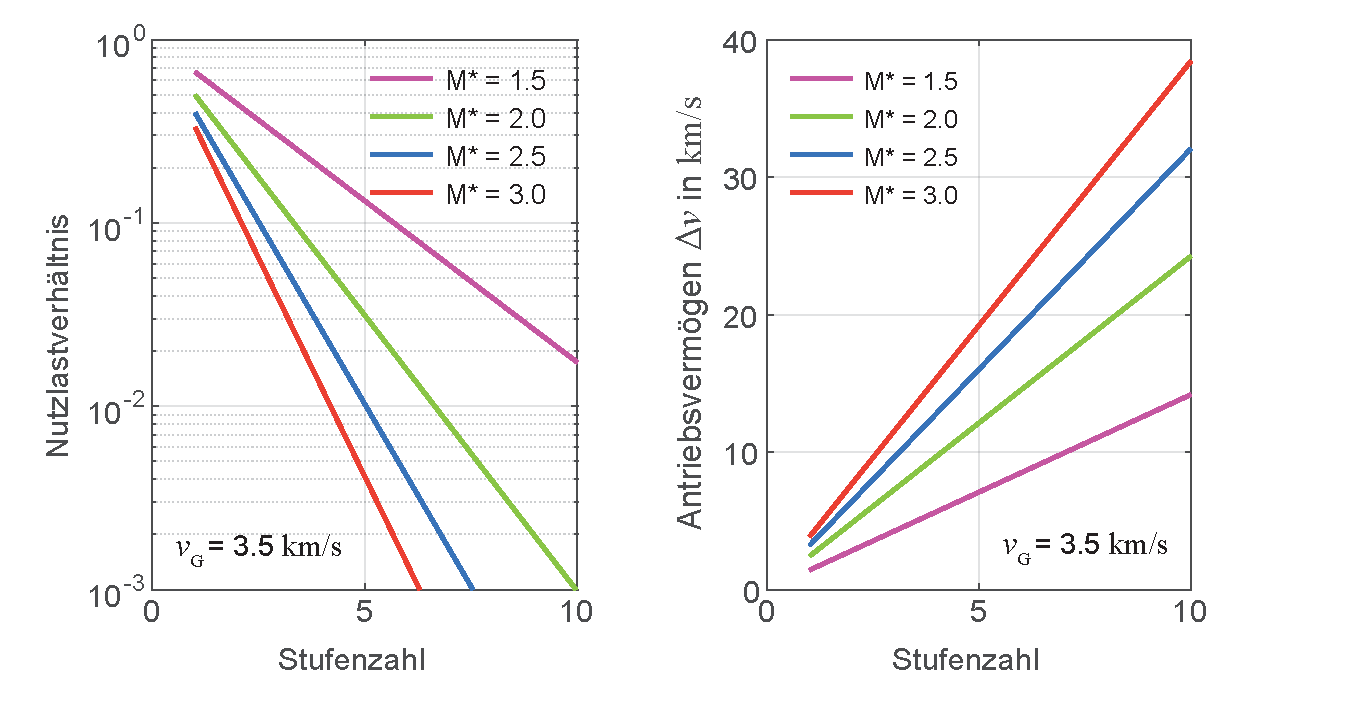
\includegraphics[width=\textwidth]{MehrStufenTheorie.pdf} 
	\caption[Nutzlastverh�ltnis �ber Antriebsbudget f�r mehrstufige Raketen.]{Nutzlastverh�ltnis �ber Antriebsbudget f�r mehrstufige Raketen bei gleichen $v_{\text{G},i}= v_\text{G}{}^*$ und 
	gleichen Struktur- und Treibstoffmassen aller Unterraketen ($\mathcal{M}^* = m_{0,i}/(m_{0,i}-m_{\text{T},i})$). Siehe \matlab{}-Datei
\mladynref{Raketenstart04.m}.}
	\label{abb:adyn_rocket_lsg05}
\end{figure}

\end{sol} 
\textcolor{blue} {$\rightarrow$ zur} \probref{adyn_rocketbasic}.\\
\noindent\rule[1ex]{\textwidth}{0.5pt}  \newpage  \clearpage

%-----------------------------------------------------------------------------------------------------------


\begin{sol}{prob:adyn_rocketopt1}\label{lsg:adyn_rocketopt1} %�bung3
\textbf{Optimierung Mehrstufenrakete (Tandemstufung)}\\
\begin{enumerate}
	\item \textit{\textbf{L�sungsansatz �ber Extremwertberechnung - Beispiel Saturn V Maximalleistung 100 t Nutzlast}}\\ 
Wir starten von der Raketen-Gleichung f�r die Tandemstufung \eqref{eq:adyn_rockets19} und fordern, dass f�r ein Nutzlastverh�ltnis
\begin{align}
    \Delta v = \sum\limits_{i_1}^N \Delta v_i = \sum\limits_{i_1}^N v_{\text{G},i}\,\ln\,\frac{1}{\sigma_i + \frac{\mu_{i+1}}{\mu_i}}\,.\label{eq:adyn_rocketsopt01} ~~~~ \rightarrow ~~~~ \text{max}
\end{align}
gelten soll. Die Bedingung f�r das Maximum lautet, wenn $\mu_\text{L}$ und alle $\sigma_i$ gegeben sind:
\begin{align}
    \frac{\d \Delta v\lk\mu_2,\mu_3,\ldots,\mu_N\rk}{\d \mu_i} = 0 ~~~~ \text{f�r} ~~~~i= 2,3,\ldots,N\,.\label{eq:adyn_rocketsopt02}
\end{align}
Daraus folgt sofort:
\begin{align}
    \frac{\d}{\d\mu_i}\,\lek -v_{\text{G},i-1}\,\ln\lk\sigma_{i-1} + \frac{\mu_i}{\mu_{i-1}}\rk- v_{\text{G},i}\,\lk\sigma_i + \frac{\mu_{i+1}}{\mu_i}\rk\rek= 0\,.\label{eq:adyn_rocketsopt03}
\end{align}
Wir f�hren  die Ableitung aus und erhalten $N-1$ Gleichungen in $\mu_i$ der Form: ($i=2,3,\ldots,N$)
\begin{align}
    \mu_i{}^2 = \frac{\lk v_{\text{G},i}-v_{\text{G},i-1}\rk\,\mu_{i+1}}{v_{\text{G},i-1}\,\sigma_i}\,\mu_i-\frac{v_{\text{G},i}}{v_{\text{G},i-1}}\,\frac{\sigma_{i-1}}{\sigma_i}\,\mu_{i-1}\,\mu_{i+1} = 0 \,,\label{eq:adyn_rocketsopt04}
\end{align}
\bzw aufgel�st nach
\begin{align}
    \mu_i = Q_i\,\mu_{i+1}+\sqrt{\lk Q_i\,\mu_{i+1}\rk^2 + P_i\,\mu_{i+1}\,\mu_{i-1}}\label{eq:adyn_rocketsopt05}
\end{align}
mit 
\begin{subequations}
\begin{align}
    Q_i = \frac{v_{\text{G},i}-v_{\text{G},i-1}}{2\,v_{\text{G},i-1}\,\sigma_i} \label{eq:adyn_rocketsopt06a}
\end{align}
und
\begin{align}
    P_i = \frac{v_{\text{G},i}\,\sigma_{i-1}}{v_{\text{G},i-1}\,\sigma_i}\;. \label{eq:adyn_rocketsopt06b}
\end{align}
\end{subequations}
F�r eine zweistufige Rakete ist $N=2$ und damit gibt es nur eine Bestimmungsgleichung f�r $\mu_2$ (da $\mu_1=1$ und $\mu_3 = \mu_L$):
\begin{align}
    \mu_2 = Q_2\,\mu_\text{L} + \sqrt{\lk Q_2\,\mu_\text{L}\rk^2 + P_2\,\mu_\text{L}}\,. \label{eq:adyn_rocketsopt07}
\end{align}
F�r eine dreistufige Rakete  ($N=3$) gibt es zwei Bestimmungsgleichungen
\begin{subequations}
\begin{align}
    \mu_2 &=  Q_2\,\mu_3 + \sqrt{\lk Q_2\,\mu_3\rk^2 + P_2\,\mu_3}\,, \label{eq:adyn_rocketsopt08a}\\
    \mu_3 &= Q_3\,\mu_\text{L} + \sqrt{\lk Q_3\,\mu_\text{L}\rk^2 + P_3\,\mu_\text{L}\,\mu_2}\,, \label{eq:adyn_rocketsopt08b}
\end{align}
\end{subequations}
die man am besten numerisch in \matlab{}  nach $\mu_2$ und $\mu_3$ l�st (siehe \mscr{} \mladynref{RaketenOptimierung01.m}). F�r $N=3$ f�hrt das Gleichungssystem 
nach einiger Algebra auf eine noch analytisch l�sbare kubische Gleichung f�r $\mu_3$, die wir hier angeben:
\begin{align*}
    \mu_3^3 - B\,\mu_3^2 + C\,\mu_3 - D &= 0 \\
		\text{mit}~~ B &= 2\mu_\text{L}\,(2Q_3+ Q_2\,P_3)\,,\\
		             C &= 4Q_3\,\mu\text{L}^2\,(Q_3+Q_2\,P_3)\,,\\
								 D &= P_2\,P_3{}^2\, \mu\text{L}^2\,.
\end{align*}
In \figref{adyn_optrockets01}a haben wir die Massenverh�ltnisse $\mu_2,\,\mu_3$ der einzelnen Raketenstufen f�r den Fall einer zweistufigen und einer dreistufigen Rakete �ber dem Nutzlastverh�ltnis aufgetragen. In \figref{adyn_optrockets01}b ist das mit heutigen Werten f�r $v_\text{G}$ maximal erzielbare Antriebsverm�gen f�r eine Stufenzahl von $N=2$ und $N=3$ �ber das Nutzlastverh�ltnis aufgetragen. Man erkennt daraus, dass man mit einer zweistufigen Rakete nicht zum Mond kommt, da $\Delta v$ kleiner als die 2.\,\gls{vkosmos} ist. \\

\begin{figure}[H]
	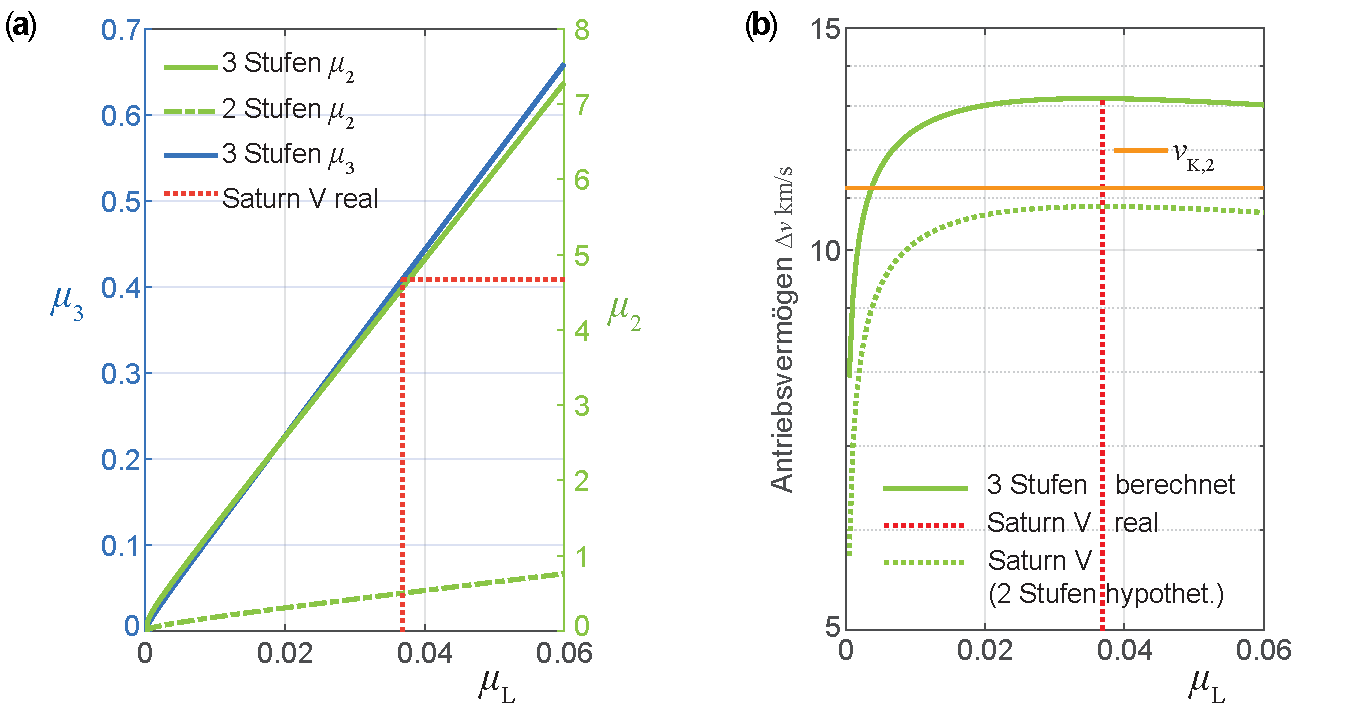
\includegraphics[width=\textwidth]{RaketenOptimierung01.pdf} 
	\caption[Optimierung einer Dreistufen-Rakete.]{Optimierung einer Dreistufen-Rakete. L�sung �ber Extremwertberechnung. \fa Berechnung der Massenverh�ltnisse der einzelnen Raketenstufen \fb Antriebsverm�gen f�r eine Dreistufen-Rakete (berechnet) und f�r die Saturn V. Zum Vergleich sind auch die Werte f�r eine (hypothetische) Ausf�hrung der Saturn V als Zweistufen-Rakete gezeigt.}
	\label{abb:adyn_optrockets01}
\end{figure}

\item \textit{\textbf{L�sungsansatz �ber Lagrange-Multiplikatoren - Beispiel Saturn V zum Mond}}\\ 
	
	Gegeben seien nach Aufgabenstellung: $v_{\text{G},i}$ (Ausstr�mgeschwindigkeit), $\sigma_i$ (Strukturparameter) und $m_0$ (Gesamtmasse der Rakete) \\
Variiert werden k�nnen die Massenverh�ltnisse $\mu_i$ oder, was gleichbedeutend ist, die Teil-Nutzlastverh�ltnisse $\eta_i$, die wir �ber
\begin{align}
    \eta_i = \frac{m_{\text{L},i}}{m_{0,i}-m_{0,i+1}} = \frac{m_{0,i+1}}{m_{\text{S},i} + m_{\text{T},i}} \label{adyn_optrocket11}
\end{align}
definieren. \\
Als $i$-tes Nutzlastverh�ltnis wird die Masse der n�chsten $\lk i+1\rk$-ten Unterrakete im Verh�ltnis zur Summe von Struktur- und Treibstoffmasse der $i$-ten Stufe definiert. Die Zahl der Stufen k�nnte ebenfalls variiert werden, soll aber hier festgehalten werden. \\
Zu optimieren/maximieren sind das Gesamt-Nutzlastverh�ltnis $\mu_\text{L}$ und das Gesamt-Antriebsverm�gen $\Delta v$, also max $\mu_\text{L}\lk \Delta v\rk$ \bzw max $\Delta v\lk\mu_\text{L}\rk $.\\
In Kapitel �ber den Lagrange-Formalismus im Band I hatten wir die Methode der Lagrange-Multiplikatoren kennen gelernt, mit der man die Extremwertberechnung der Wirkung $S$ bei Vorliegen von Zwangsbedingungen \bzw Nebenbedingungen durchf�hren konnte. Wir wenden dies f�r unser Problem an. Der Wirkung $S$ entspricht hier die Gr��e $\mu_\text{L}$ \bzw $\Delta v$, die Nebenbedingungen sind duch die $m_{\text{S},i}$ \bzw $\sigma_{i}$ gegeben und die "`Bewegungsgleichungen"' ergeben sich dann durch:
\begin{align}
    \frac{\d\lk\mu_\text{L}\rk}{\d \eta_j} + \lambda_{\mu_\text{L}}\,\frac{\d\lk \Delta v\rk}{\d \eta_j} = 0 ~~~~ \text{(maximieren von $\mu_\text{L}$)} \label{adyn_optrocket12}
\end{align}
\bzw
\begin{align}
    \frac{\d\lk\Delta v\rk}{\d \eta_j} + \lambda_{\Delta v}\,\frac{\d\lk \mu_\text{L}\rk}{\d \eta_j} = 0 ~~~~ \text{(maximieren von $\Delta v$)} \,.\label{adyn_optrocket13}
\end{align}
F�r $\lambda_{\mu_\text{L}} = 1/\lambda_{\Delta v}$ beschreiben beide Gleichungen das gleiche mathematische Problem.\\
Wir f�hren die Ableitungen aus und erhalten:
\begin{align}
\begin{split}
     \frac{\d\lk\Delta v\rk}{\d \eta_j} &= -v_{\text{G,j}}\,\frac{1-\sigma_j}{1+\eta_j}\,\frac{1}{\sigma_j+\eta_j} \,,\\
     \frac{\d\lk\mu_\text{L}\rk}{\d \eta_j}  &= \frac{\mu_\text{L}}{\eta_j\lk 1+\eta_j\rk}
\end{split}\label{adyn_optrocket14}
\end{align}
und erhalten aus \eqref{adyn_optrocket12}
\begin{align}
    \frac{\mu_\text{L}}{\eta_j\lk 1+\eta_j\rk} = \lambda_{\mu_\text{L}}\,v_{\text{G},j}\,\frac{1-\sigma_j}{1+\eta_j}\,\frac{1}{\sigma_j + \eta_j} \label{adyn_optrocket15} \,.
\end{align}
Daraus folgt sofort
\begin{align}
    v_{\text{G},j}\,\eta_j\,\frac{1-\sigma_j}{\sigma_j + \eta_j} = \frac{\mu_\text{L}}{\lambda_{\mu_\text{L}}} =:\gamma = \text{const} ~~~~ j=1,2,\ldots,N \,.\label{adyn_optrocket16}
\end{align}
Damit haben wir die Grundgleichungen f�r die Optimierung. \\
$\gamma$ ist noch eine unbekannte Gr��e, die es aus \eqref{adyn_optrocket16} zu bestimmen gilt. Wir nehmen diese zun�chst als bestimmt an, so dass sich dann die optimalen Nutzlastverh�ltnisse ergeben zu:
\begin{align}
    \eta_\text{j,\text{opt}} = \frac{\gamma\,\sigma_j}{\lk 1-\sigma_j\rk\,v_{\text{G},j}-\gamma}~~~~ j=1,2,\ldots,N \,.\label{adyn_optrocket17}
\end{align}
Wir setzen diese in die Raketen-Gleichung f�r die serielle Stufung \eqref{eq:adyn_rockets17} ein und erhalten:
\begin{align}
    \Delta v = \sum\limits_{j=1}^N\,v_{\text{G},j}\,\ln\,\frac{1+\eta_j}{\sigma_j + \eta_j} = \sum\limits_{j=1}^Nv_{\text{G},j}\,\ln\,\frac{v_{\text{G},j}-\gamma}{\sigma_j\,v_{\text{G},j}}\,.\label{adyn_optrocket18}
\end{align}
F�r das totale Nutzlastverh�ltnis 
\begin{align}
    \mu_\text{L} = \frac{m_\text{L}}{m_0} = \prod\limits_{j=1}^N\frac{\eta_j}{1+\eta_j} = \prod\limits_{j=1}^N \frac{\gamma\,\sigma_j}{\lk 1-\sigma_j\rk\lk v_{\text{G},j}-\gamma\rk}\,.\label{adyn_optrocket19}
\end{align}
Der weitere Weg besteht darin, dass man aus \eqref{adyn_optrocket18} f�r bekannte $\sigma_j$, $\Delta v$ die Konstante $\gamma$ (die aus dem Lagrange-Multiplikator abgeleitet wurde) bestimmt und diese in \eqref{adyn_optrocket19} einsetzt, um $\mu_\text{L,opt}$ zu erhalten. \\
Die Konstante $\gamma$ muss aus der Gleichung \eqref{adyn_optrocket16} numerisch bestimmt werden, was wir vorteilhaft in \matlab\,im Skript \mladynref{RaketenOptimierung02.m} ausgef�hrt haben.\\
Wenn wir die in der �bung in Tabelle \ref{tab:adyn_parameter_Apollo11} angegebenen Werte verwenden, erhalten wir aus der Rechnung einen Wert von $\mu_\text{L} = 0.0176$, der nur wenig von dem tats�chlichen (etwas kleineren) Wert von $\mu_\text{L} = 0.0162$ abweicht, mit dem die NASA (vermutlich aus Sicherheitsgr�nden) operierte.
In \figref{adyn_optrockets02} ist das maximale Nutzlastverh�ltnis gezeigt, mit der eine Nutzlast von $m_\text{L} = \mu_\text{L,opt}\cdot m_0$ auf ein bestimmtes Antriebsverm�gen gebracht werden kann.\\
Es sei noch darauf hingewiesen, dass $\gamma < \mathrm{min}\lk v_{\text{G},j}\,\lk 1-\sigma_j\rk \rk \,$f�r alle $j=1,\ldots,N$ sein muss, was bei der numerischen Berechnung zu ber�cksichtigen ist.
	
\begin{figure}[H]
	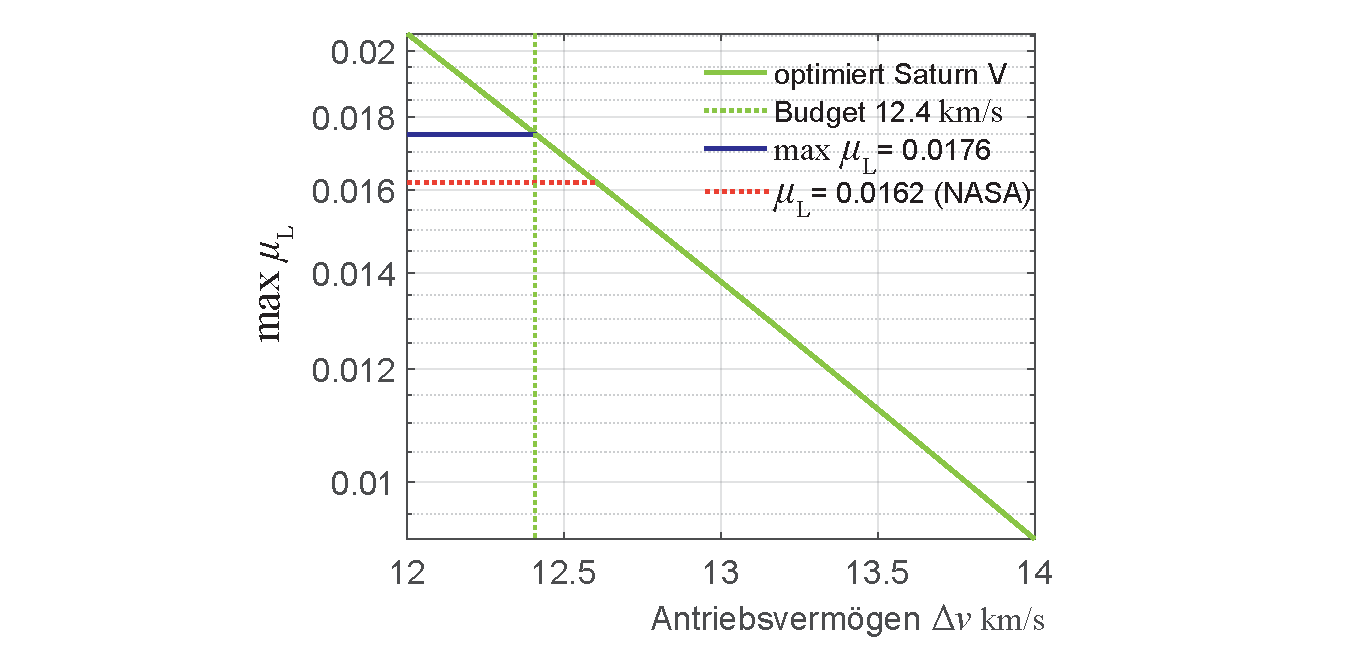
\includegraphics[width=\textwidth]{RaketenOptimierung02.pdf} 
	\caption[Optimierung einer Dreistufen-Rakete.]{Optimierung Saturn V Konfiguration f�r die Apollo Missionen. L�sung �ber Methode der Lagrange-Multiplikatoren. Berechnung des optimalen Antriebsverm�gens/Nutzlastverh�ltnisses.}
	\label{abb:adyn_optrockets02}
\end{figure}


\end{enumerate}

\end{sol} 
\textcolor{blue} {$\rightarrow$ zur} \probref{adyn_rocketopt1}.\\
\noindent\rule[1ex]{\textwidth}{0.5pt}  \newpage  \clearpage


%-----------------------------------------------------------------------------------------------------------


\begin{sol}{prob:adyn_rocketopt2}\label{lsg:adyn_rocketopt2} %�bung4
\textbf{Vergleich Mehrstufenrakete (Serielle und Parallelstufung)} \\ \\
Wir fassen die Vor- und Nachteile der Tandemstufung gegen�ber der Parallelstufung  in der folgenden Tabelle zusammen.\\
\begin{table}%tab1
\caption{Vor- und Nachteile der Tandemstufung gegen�ber der Parallelstufung.}
\smallskip
\hspace{1.5cm}
\begin{tabular}{L{3cm}L{3cm}L{3cm}}
\svhline\noalign{\smallskip}
Eigenschaft				    			& Tandemstufung				& Parallelstufung \\
\noalign{\smallskip}\svhline\noalign{\smallskip}
\noalign{\smallskip}
Startbeschleunigung							&kleiner &gr��er\\	
Strukturbelastung 							&kleiner &gr��er\\	
Biegemomente      							&gr��er  &kleiner\\	
Aerodynamische Verluste 				&kleiner &gr��er\\	
Gravitationsverluste						&gr��er  &kleiner\\	
Gesamtl�nge Rakete							&gr��er  &kleiner\\	
\noalign{\smallskip}
\svhline\noalign{\smallskip}
\end{tabular} \\
\label{tab:adyn_vergleich_staging}
\end{table}%tab1


\end{sol} 
\textcolor{blue} {$\rightarrow$ zur} \probref{adyn_rocketopt2}.\\
\noindent\rule[1ex]{\textwidth}{0.5pt}  \newpage  \clearpage


%-----------------------------------------------------------------------------------------------------------


%-----------------------------------------------------------------------------------------------------------
%-----------------------------------------------------------------------------------------------------------

\subsection{�bungen zu Umlaufbahnen}

\medskip

%-----------------------------------------------------------------------------------------------------------

\begin{sol}{prob:adyn_orbits1}\label{lsg:adyn_orbits1} %�bung5
\textbf{Bahnparameter aus Bodenbeobachtungen}\\ \\
\textit{Bahnparameter von Satelliten mit gegebenen geozentrischen Orts- und Geschwindigkeitsdaten:}\\ \\
Wir verwenden die Formeln aus \kap{adyn_orbits_determination_rv} und erhalten:\\

Satellit 1 (HEO)
\begin{align*}
	&\text{Halbachse}\,\,a & \SI{20251.57}{\km}\\
	&\text{Exzentrizit�t}\,\,e & 0.777596\\
	&\text{Bahnneigung} \,\,i &   10.194 \degree\\
	&\text{Knoten} \,\, \Omega &  171.951 \degree\\
	&\text{Arg. Perig�um} \,\, \omega &  86.081 \degree\\
	&\text{Mittl. Anomalie} \,\, M &  138.824  \degree\\
	&\text{Mittl. Bewegung} \,\, n & \SI{2.19e-04}{\per\second} \\
\end{align*}

Satellit 2 (LEO)
\begin{align*}
	&\text{Halbachse}\,\,a & \SI{8225.40}{\km}\\
	&\text{Exzentrizit�t}\,\,e & 0.076722\\
	&\text{Bahnneigung} \,\,i &   6.707 \degree\\
	&\text{Knoten} \,\, \Omega &  145.881 \degree\\
	&\text{Arg. Perig�um} \,\, \omega &  86.476 \degree\\
	&\text{Mittl. Anomalie} \,\, M &  167.278  \degree\\
	&\text{Mittl. Bewegung} \,\, n & \SI{8.46e-04}{\per\second}
\end{align*}

\newpage

\textit{Bahnparameter der ISS aus den ver�ffentlichten geozentrischen Orts- und Geschwindigkeitsdaten der NASA:}\\
	%\url{https://spotthestation.nasa.gov/trajectory_data.cfm}\\

Auch hier verwenden wir die Formeln aus \kap{adyn_orbits_determination_rv} und erhalten:
\begin{align*}
	&\text{Halbachse}\,\,a & \SI{6803.28}{\km}\\
	&\text{Bahnh�he}\,\,h & \SI{425.28}{\km}\\
	&\text{Exzentrizit�t}\,\,e & 0.001855\\
	&\text{Bahnneigung} \,\,i &  51.751 \degree\\
	&\text{Knoten} \,\, \Omega &  47.685 \degree\\
	&\text{Arg. Perig�um} \,\, \omega & 124.00 \degree\\
	&\text{Mittl. Anomalie} \,\, M & 315.75 \degree\\
	&\text{Umlaufzeit} \,\, n & \SI{93.8 }{\minute}
\end{align*}
Die mittlere Anomalie $M$ wurde so angepasst, dass der Anfangswert mit den NASA Daten �bereinstimmt. Wir verweisen auf \kap{adyn_orbits_determination_singulaer}
zur Berechnung alternativer Bahnparameter bei kreisf�rmigen und �quatorialen Bahnen, sowie auf die Zusatzaufgabe \probref{adyn_orbits_zusatz1}.
\begin{figure}[H]
	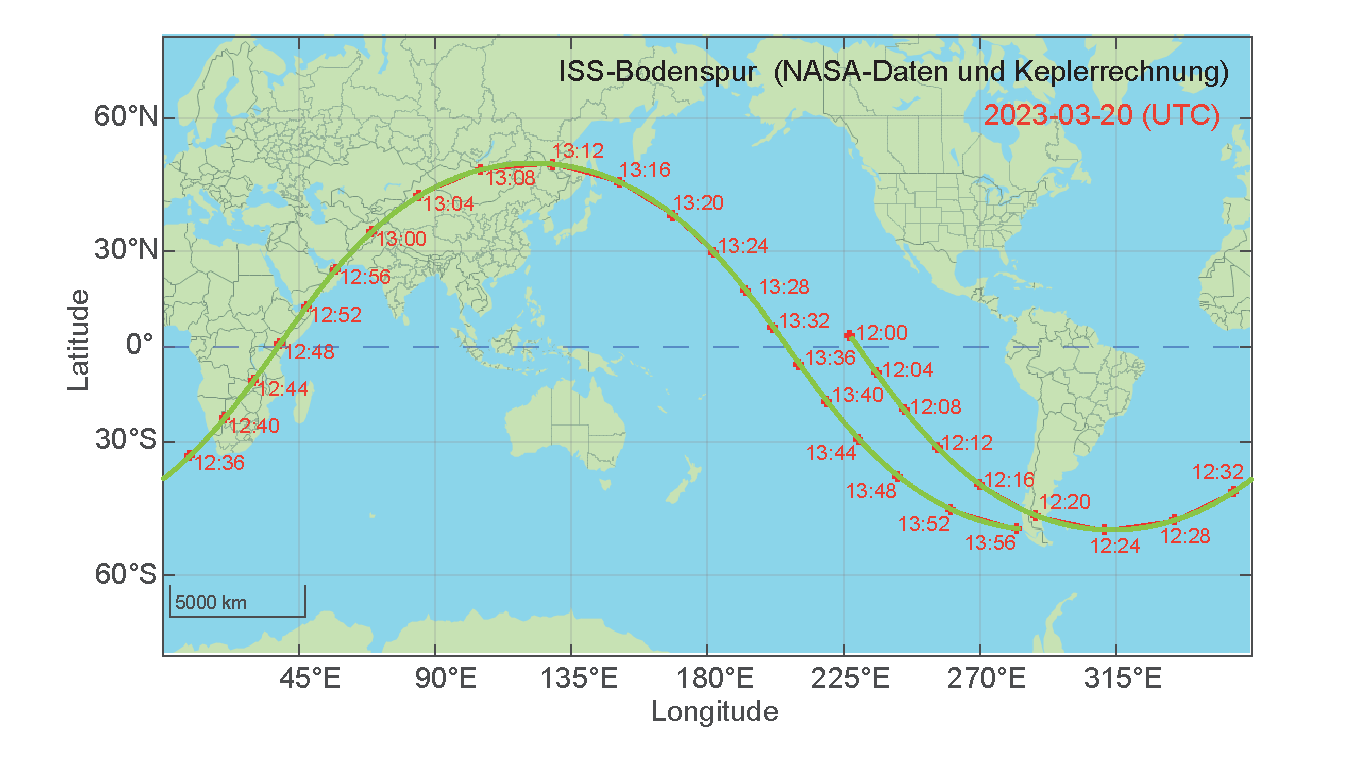
\includegraphics[width=\textwidth]{GroundTrackISS20032023.pdf} 
	\caption[Bodenspur der ISS.]{Bodenspur der ISS. Vergleich NASA Daten und Berechnung Keplerbahn.}
	\label{abb:adyn_satobserv02}
\end{figure}
Die Berechnungen finden sich im Detail im \mscr{} \mladynref{BahnparaBestimmung01.m}. 

\end{sol} 
\textcolor{blue} {$\rightarrow$ zur} \probref{adyn_orbits1}.\\
\noindent\rule[1ex]{\textwidth}{0.5pt}  \newpage  \clearpage

%-----------------------------------------------------------------------------------------------------------
\newpage

\begin{sol}{prob:adyn_orbits2}\label{lsg:adyn_orbits2} %�bung6
\textbf{Bodenspuren von Erdsatelliten}\\ 

\begin{itemize}
	\item \textit{\textbf{Bodenspuren verschiedener Satellitenarten}}\\
		\begin{itemize}
			\item Bodenspur eines GEO-Satelliten.
			\item Bodenspur eines Molnija-Satelliten (HEO-Satelliten).
			\item Bodenspur eines polaren Satelliten. 
		\end{itemize}
		\begin{figure}[H]
			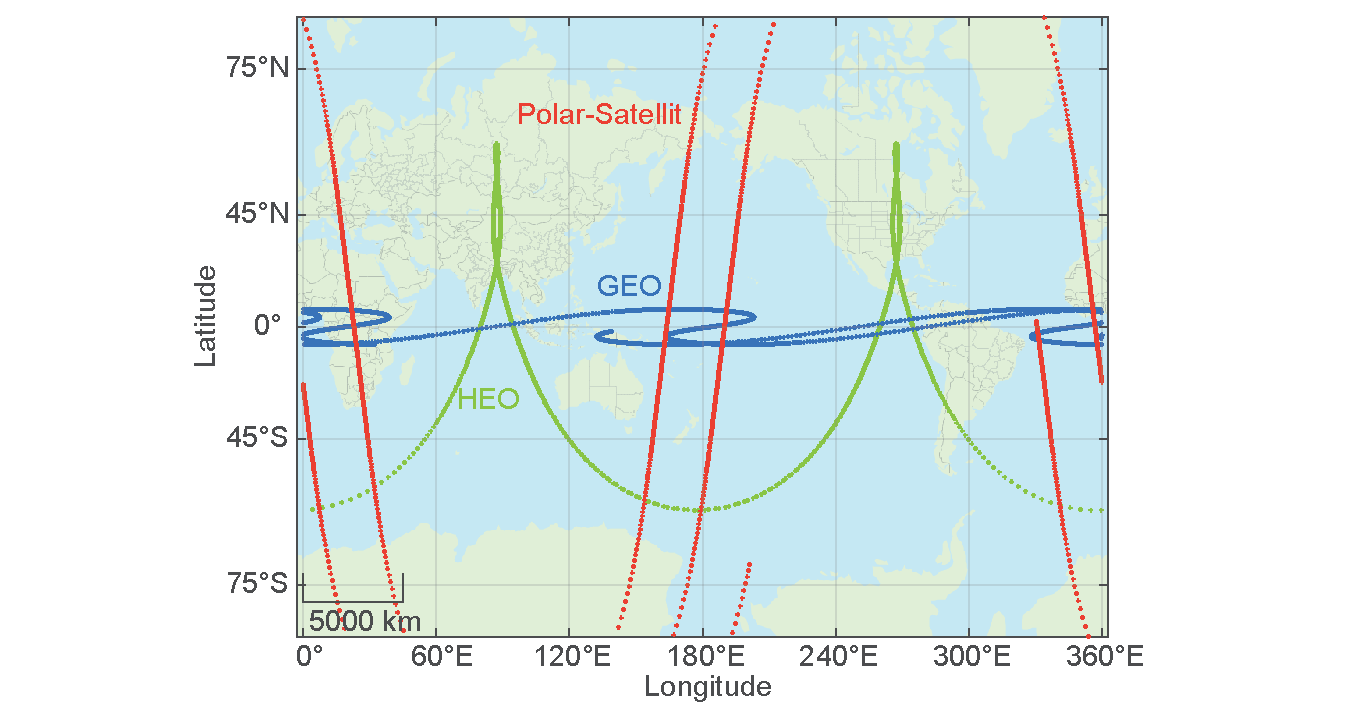
\includegraphics[width=0.9\textwidth]{Orbits03a.pdf} 
			\caption[Bodenspuren von verschiedenen Satelliten.]{Bodenspuren von verschiedenen Satelliten. GEO:\, $a = \SI{25000}{\km},\, e = 0.73,\, i = 8\degree,\, \Omega =45\degree$,\,\, HEO (Typ Molnija-Satelliten):\, $a = \SI{26555}{\km},\, e = 0.72,\, i = 63.4\degree,\, \Omega =120\degree,\,\omega =270\degree$,\,\, Polar-Satellit:\, $a = \SI{7330}{\km},\, e = 0.0,\, i = 93\degree,\, \Omega =130\degree,\,\omega =0\degree$.}
			\label{abb:adyn_orbits03a}
			\end{figure}
	\item \textit{\textbf{Bodenspuren verschiedener Satelliten in geosynchronen Umlaufbahnen}}\\

				Die Bodenspuren \figref{adyn_orbits03b} �hneln den verschiedenen Analemma, die wir im \kap{kulmination_sonne} \bzw in der \probref{hm_Analemma_Mars} kennen gelernt hatten. Das ist nicht verwunderlich. In einer geozentrischen Betrachtung �bernehmen die Satelliten die Rolle der Sonne, die unterschiedlichen Formen des \textit{\anf{Satelliten-Analemmas}} kommen durch die unterschiedlichen Bahnparameter zustande. Siehe auch im Detail \probref{hm_Analemma_Mars}.\\
\newpage
			\begin{figure}[H]
			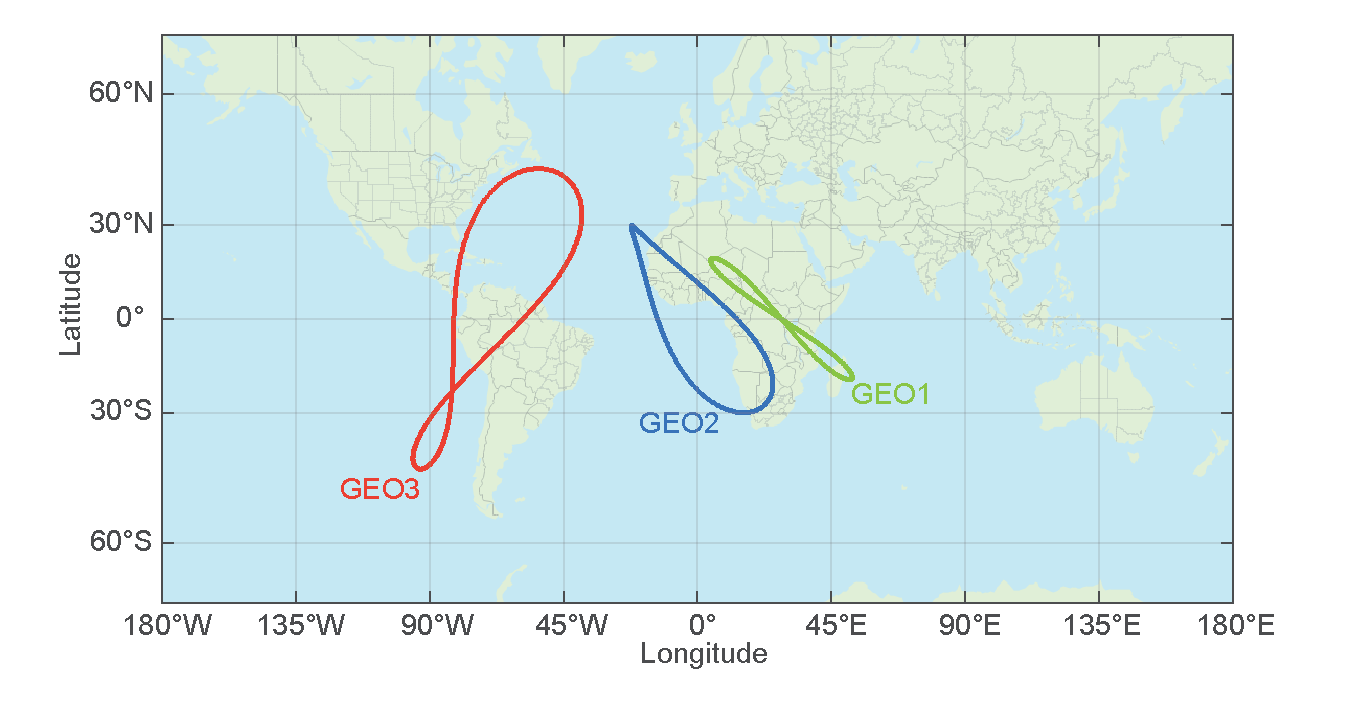
\includegraphics[width=0.95\textwidth]{Orbits03b.pdf} 
			\caption[Bodenspuren von verschiedenen geosynchronen Satelliten.]{Bodenspuren von verschiedenen geosynchronen Satelliten. Parameter siehe \probref{adyn_orbits2}.}
			\label{abb:adyn_orbits03b}
			\end{figure}
\item \textit{\textbf{Bodenspur ISS}}\\
			\begin{figure}[H]
			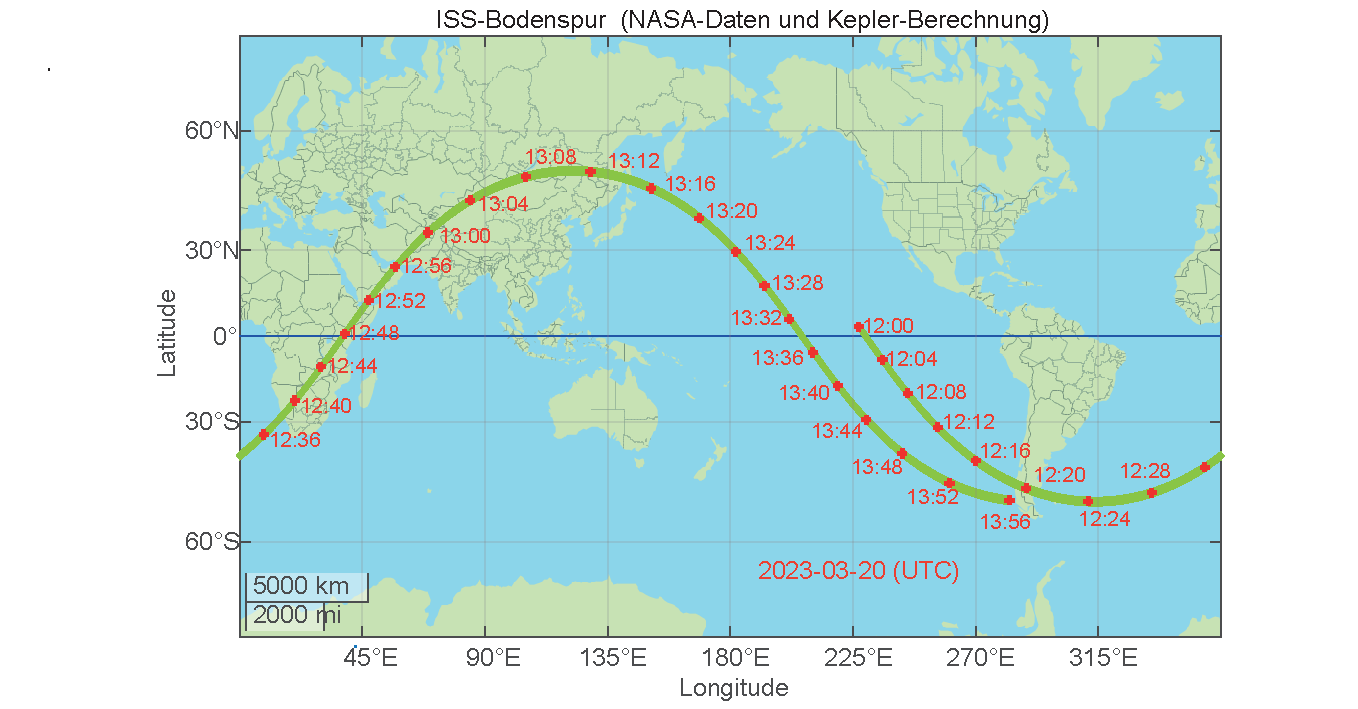
\includegraphics[width=0.95\textwidth]{ISSBodenspur.pdf} 
			\caption[Bodenspuren der ISS.]{Bodenspuren der ISS vom 20.03.2023. Parameter siehe \probref{adyn_orbits2}.}
			\label{abb:adyn_orbits03c}
			\end{figure}
\end{itemize}
Die Berechnungen finden sich im Detail im \mscr~\mladynref{SatPositionen01.m} \bzw \mladynref{SatPositionen02.m}.

\end{sol} 
\textcolor{blue} {$\rightarrow$ zur} \probref{adyn_orbits2}.\\
\noindent\rule[1ex]{\textwidth}{0.5pt}  \newpage  \clearpage

%-----------------------------------------------------------------------------------------------------------

\begin{sol}{prob:adyn_orbits3}\label{lsg:adyn_orbits3} %�bung7
\textbf{Bodenbeobachtung von Erdsatelliten}\\ \\

Die Berechnungen finden sich im Detail im \mscr~\mladynref{SatPositionen03.m} \bzw \mladynref{SatPositionen04.m}.
\begin{figure}[H]
	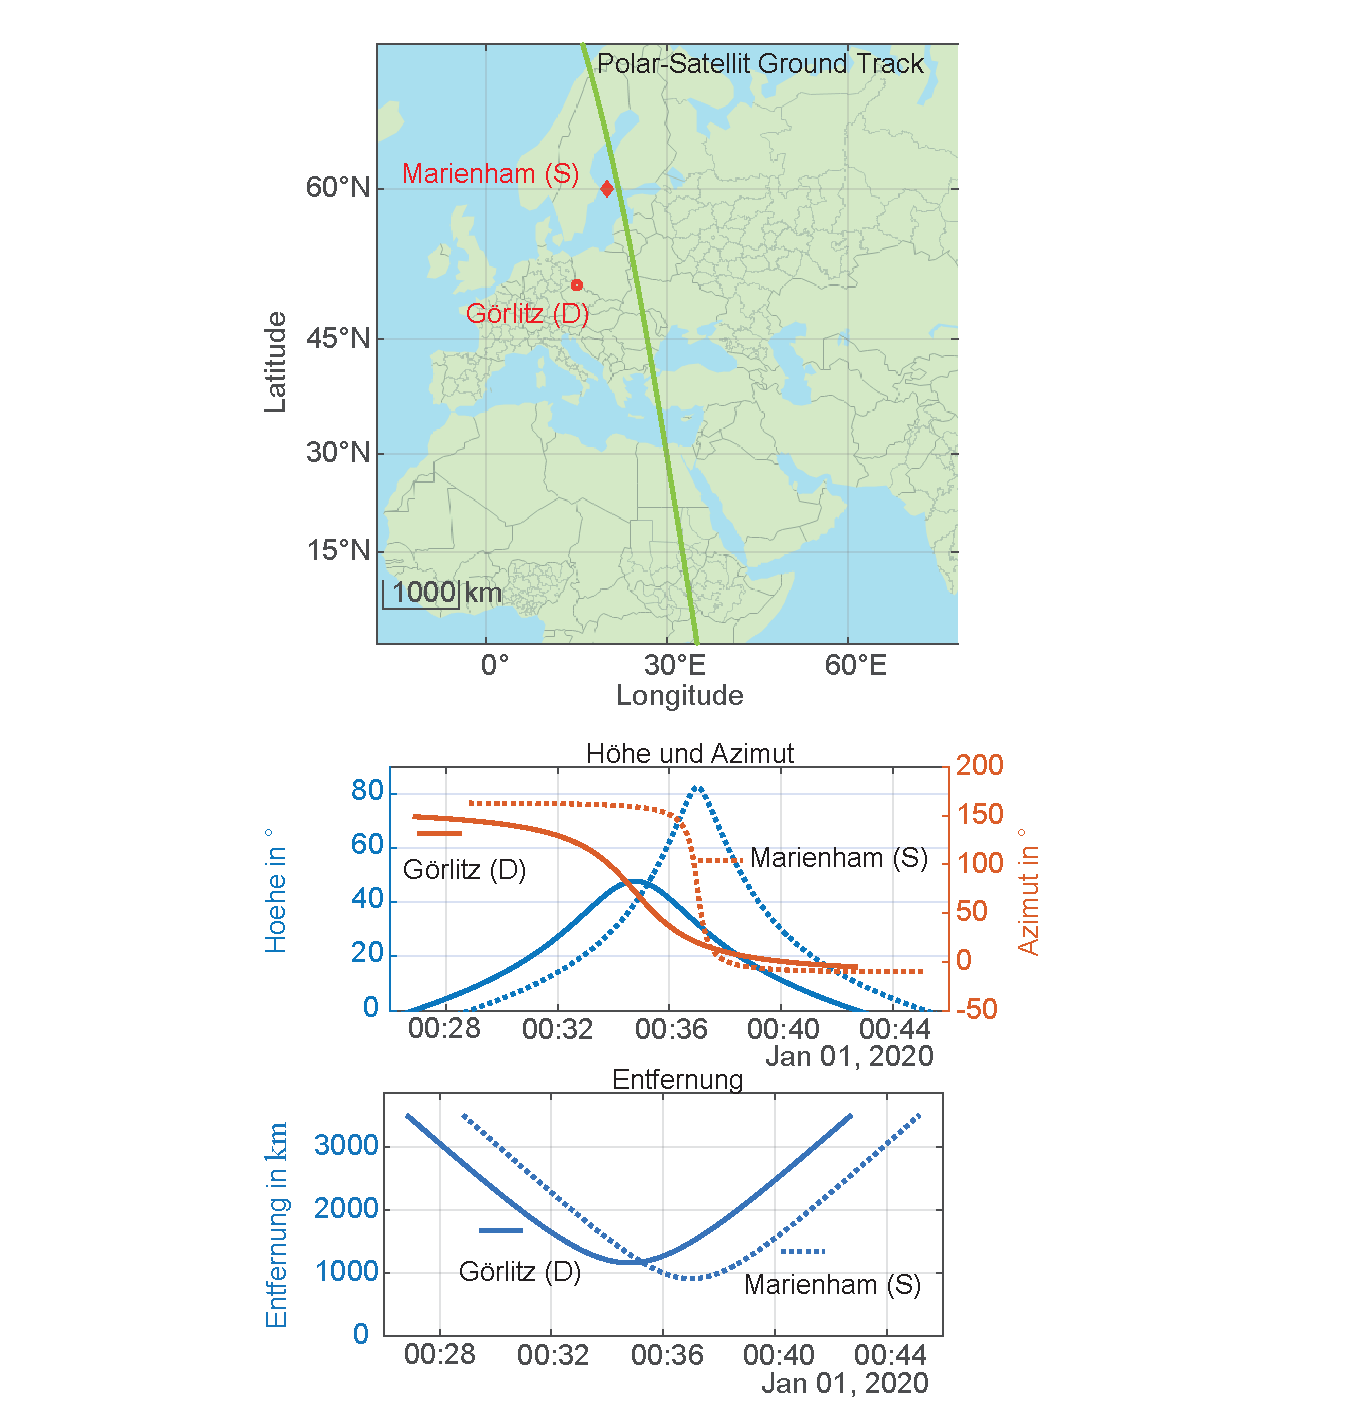
\includegraphics[width=\textwidth]{TopographPolarerSat.pdf} 
	\caption[Topographische Beobachtung eines polaren Satelliten.]{Bodenspur, Azimut, H�he und Entfernung eines polaren Satelliten von zwei Bodenstationen. Parameter siehe \probref{adyn_orbits3} und \mscr~\mladynref{SatPositionen03.m} \bzw \mscr~\mladynref{SatPositionen03a.m}.}
	\label{abb:adyn_satobserv03}
\end{figure}
\begin{figure}[H]
	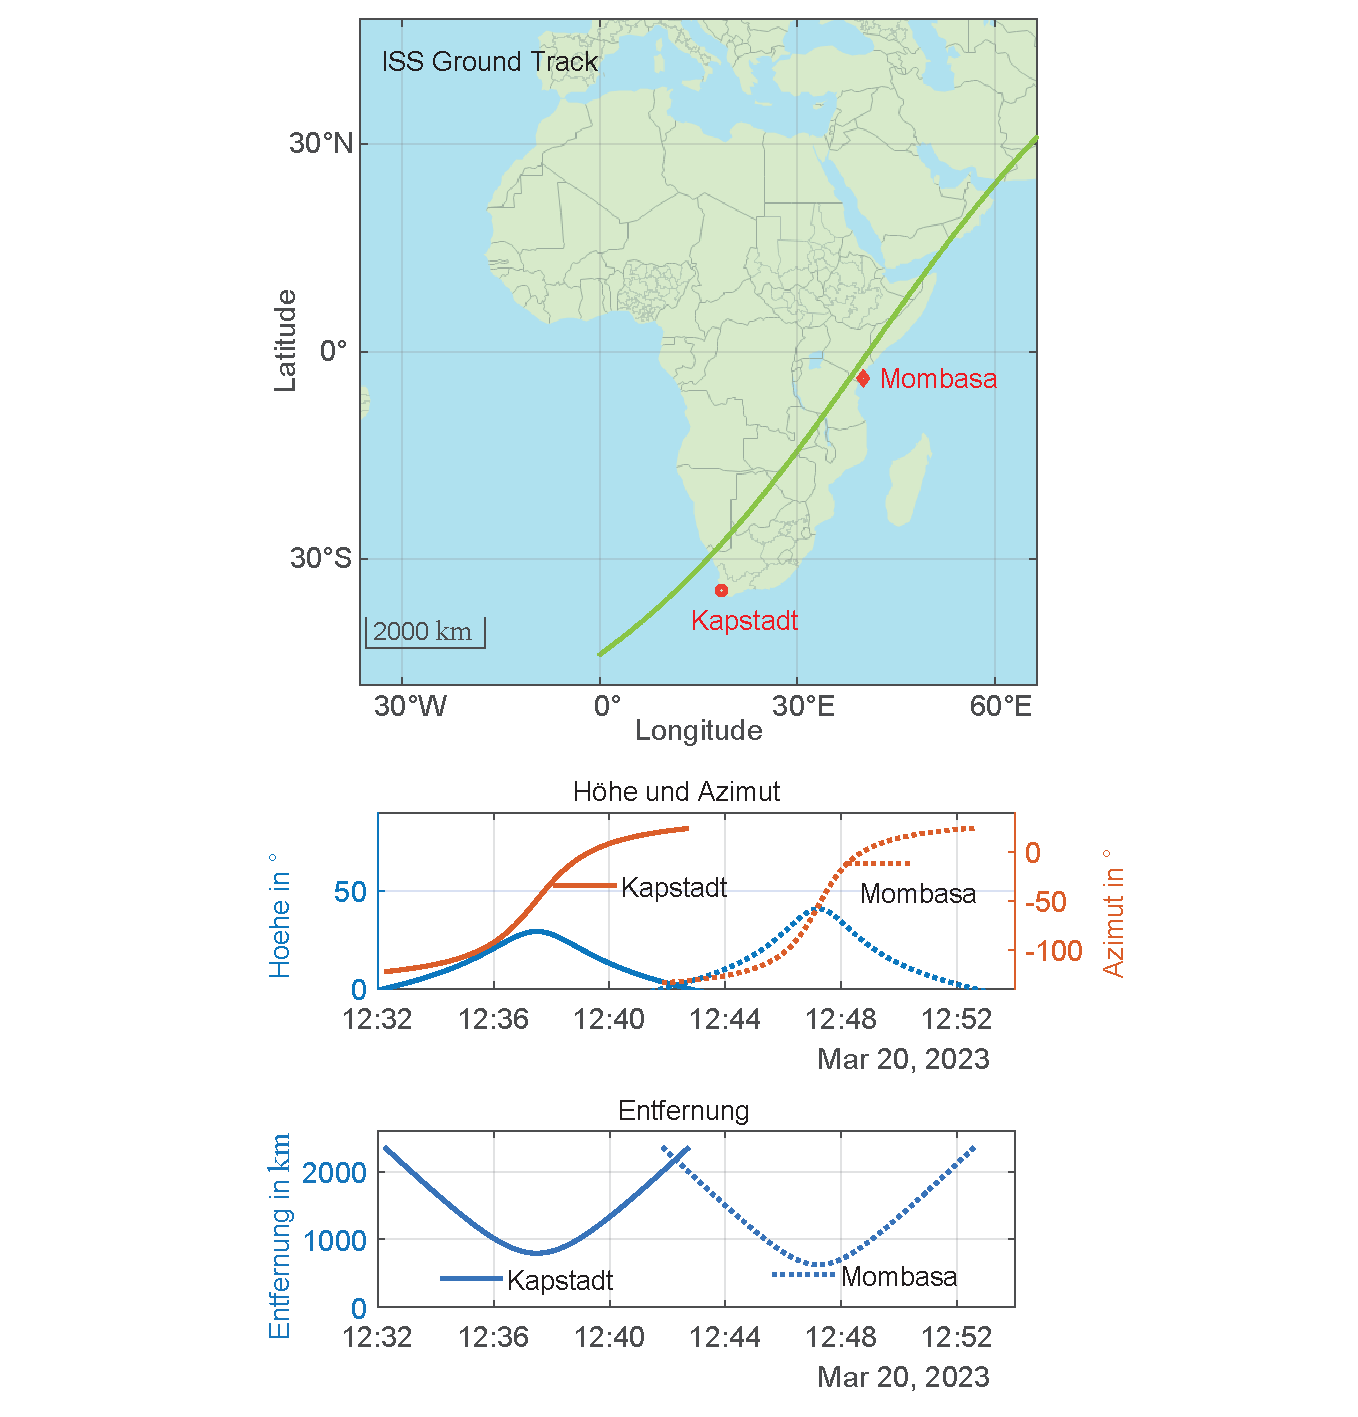
\includegraphics[width=\textwidth]{TopographISS.pdf} 
	\caption[Topographische Beobachtung der ISS.]{Bodenspur, Azimut, H�he und Entfernung der von zwei Bodenstationen. Parameter siehe \probref{adyn_orbits3} und \mscr~\mladynref{SatPositionen04.m}.}
	\label{abb:adyn_satobserv04}
\end{figure}

\end{sol} 
\textcolor{blue} {$\rightarrow$ zur} \probref{adyn_orbits3}.\\
\noindent\rule[1ex]{\textwidth}{0.5pt}  \newpage  \clearpage

%-----------------------------------------------------------------------------------------------------------

\begin{sol}{prob:adyn_orbits4}\label{lsg:adyn_orbits4} %�bung8
\textbf{Bodenbeobachtung eines Molniya-Satelliten}\\ \\

Die Berechnungen finden sich im Detail im \mscr~\mladynref{SatPositionen05.m}.
\begin{figure}[H]
	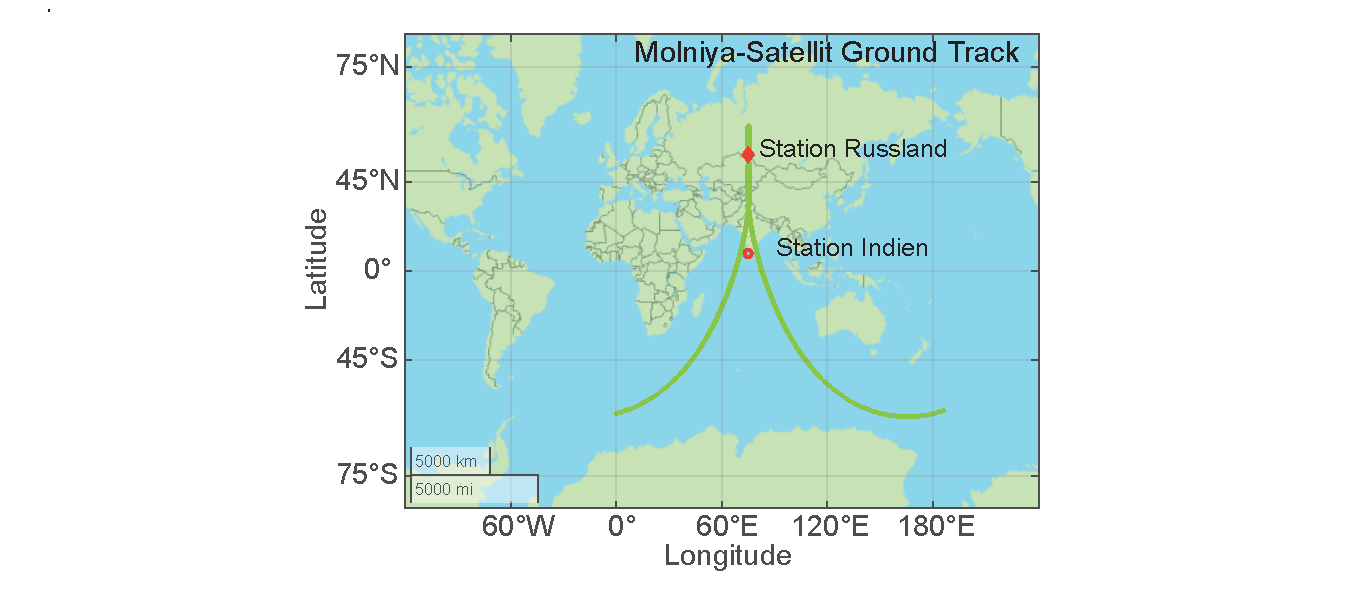
\includegraphics[width=\textwidth]{TopographMolniyaSat01.pdf} 
	\caption[Bodenspur eines Molniya-Satelliten.]{Bodenspur eines Molniya-Satelliten.\\Parameter siehe \probref{adyn_orbits4} und \mscr~\mladynref{SatPositionen05.m}.}
	\label{abb:adyn_MolniyaObserv01}
\end{figure}
\begin{figure}[H]
	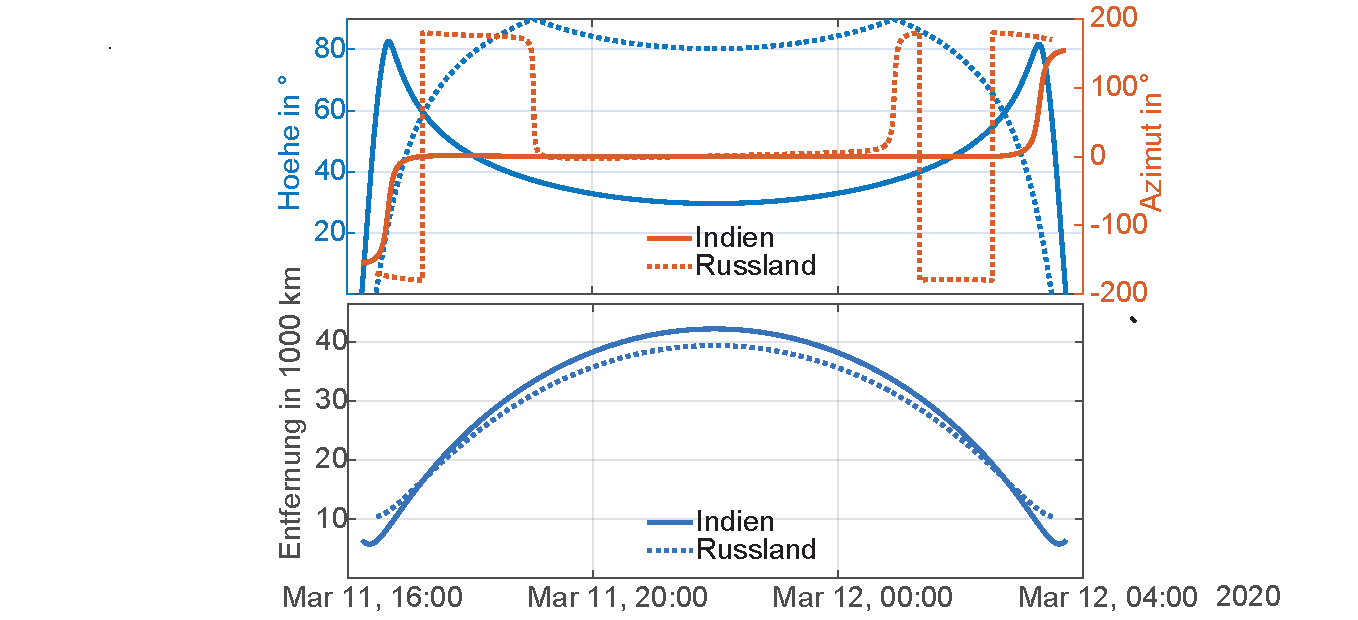
\includegraphics[width=\textwidth]{TopographMolniyaSat02.pdf} 
	\caption[Topographische Beobachtung eines Molniya-Satelliten.]{Azimut, H�he und Entfernung eines Molniya-Satelliten von zwei Bodenstationen. Parameter siehe \probref{adyn_orbits4} und \mscr~\mladynref{SatPositionen05.m}.}
	\label{abb:adyn_MolniyaObserv02}
\end{figure}
\end{sol} 
\textcolor{blue} {$\rightarrow$ zur} \probref{adyn_orbits4}.\\
\noindent\rule[1ex]{\textwidth}{0.5pt}  \newpage  \clearpage


%-----------------------------------------------------------------------------------------------------------

\begin{sol}{prob:adyn_orbits5}\label{lsg:adyn_orbits5} %�bung9
\textbf{Sonnensynchrone Bahnen}\\ \\

Die Drehimpulserhaltung gilt streng nur f�r das Zweik�rperproblem, dann ist auch die Bahnebene fest im Raum orientiert und die Bahn geschlossen.\\
Wie wir \zb in \kap{Periheldrehung} gesehen haben, bewirkt die Abplattung der Erde jedoch ein Drehmoment auf die Bahn und f�hrt zu einer Verschiebung der Rektaszension des aufsteigenden Knotens. 
Man kann mit Hilfe der St�rungsrechnung zeigen (siehe auch \probref{adyn_pertubations}), dass die Frequenz dieser Pr�zession des aufsteigenden Knoten sich nach folgender Formel berechnet:
	\begin{align}
		\dot{\Omega} = -\frac{3}{2} J_2\, \frac{2\pi}{T_\text{E}} \lk \frac{R_\text{E}}{a\,(1-e^2)} \rk^2 \cos i = 
		-\frac{3}{2} J_2\,R_\text{E}\, \sqrt{\frac{a_\text{E}}{a_\text{E}{}^2}} \, \frac{\cos i}{a^2\,(1-e^2)^2} = C\,f(a,e,i)\,. \label{eq:adyn_orbits5_01}
	\end{align}
Hierin sind $J_2$ die sogenannte zonale Harmonische\index{Harmonische!zonale} (siehe \kap{adyn_gravity_pertubations}) als Ma� f�r die Abplattung der Erde, $R_\text{E}$ der mittlere Erdradius, $a$ die gro�e Halbachse der Satellitenbahn und $i$ \bzw $e$ deren Neigung (Inklination) \bzw Exzentrizit�t. $T_\text{E} = 2\pi\sqrt{a_\text{E}{}^3/\mu_\text{E}}$ ist die Umlaufzeit der Erde um die Sonne.\footnote{Genauer gesagt ist es die Zeit eines anomalistischen Jahres ($\SI{365.25963}{}\,\mathrm{d}$, siehe \kap{hm_zeitdefinition})} Die Pr�zession ist umso gr��er, je geringer die Inklination $i$ und die Bahnh�he $a$ sind.\\
Wegen des Minuszeichen wirkt bei einer retrograden Bahnen (Bahn entgegen der Erdrotation, \dh $i > 90\degree$) diese Pr�zession in die gleiche Richtung wie die Erdrotation. Man kann also durch geeigneter Wahl von Inklination und Flugh�hen daf�r sorgen, dass sich die Bahn gerade um so viel verschiebt wie der mittleren Bewegung der Erde ($2\pi/T_\text{E}$) um die Sonne entspricht (\figref{adyn_synchron_orbit}). 

Bei einem SSO erfolgt der �berflug des Satelliten �ber einen Punkt auf der Oberfl�che des Planeten immer zur selben Ortszeit, vorausgesetzt die geographische Breite des Ortes liegt innerhalb des Bereiches, der durch die Inklination der Bahn begrenzt wird. Aufgrund dieser konstanten �berflugszeit lassen sich Beobachtungen von verschiedenen Tagen und Jahreszeiten gut miteinander vergleichen, deswegen haben ja Wetter- und Erdbeobachtungssatelliten oft solche Bahnen.

\begin{figure}[H]
	\includegraphics[width=\textwidth]{SonnensynchroneBahn.pdf} 
	\caption[Sonnensynchrone Bahn.]{Sonnensynchrone Bahn. Symbolische und nicht-ma�stabsgetreue Darstellung. }
	\label{abb:adyn_synchron_orbit}
\end{figure}

\newpage
\textbf{Zusatzaufgabe}\\

Wir wollen nun noch die Bodenspur des ERS-1 SSO-Satelliten berechnen \cite{Gottschalk1991}. Man k�nnte nun aus \eqref{eq:adyn_orbits5_01} einen der Parameter $a,\, e$ oder $i$ berechnen und die anderen vorgeben. 
Man hat aber eben mit $a$ einen weiteren Freiheitsgrad neben $i$, womit man auch fordern kann, dass die Bahnh�he $h$ so gew�hlt wird, dass ein �berflug �ber eine Gebiet (\zb das �berkreuzen des �quators nach $K$ Tagen \bzw. $N$ Orbits genau wiederholt (sogenannte \textit{Sonnensynchrone Repeat Orbits}).  Anfangs w�hlte man f�r den ERS-1 K=3, N=43, sp�ter ging man auf K=35.
Um das zu erreichen, muss man auch die St�rungen der Perihelverschiebung (siehe \kap{Stoerpotential_Merkur}) und der mittleren Anomalie ber�cksichtigen. Diese sind f�r kreisf�rmige Bahnen gegeben durch \cite{Montenbruck2012, Murray2008, Vallado2007}:

	\begin{align}
	\begin{split}
		\dot{\omega} = -\frac{3}{4} J_2\, n_0 \frac{R_\text{E}{}^2}{a^2} \lk 1 - 5\cos^2 i\rk \\ 
    \Delta n = n - n0  = -\frac{3}{4} J_2\, n_0 \frac{R_\text{E}{}^2}{a^2} \lk 1 - 2\cos^2 i\rk\,,
	\end{split}\label{eq:adyn_orbits5_02}
\end{align}

worin $n_0=\sqrt{(GM_\text{E}/a^3)}$ die mittlere Bewegung der Kepler-Bahn ist.
F�r sonnensynchrone Bahnen ist dann gefordert, dass gilt:

	\begin{align}
		\dot{\Omega} - \dot{\theta} = -360\degree\,, \\ 
\label{eq:adyn_orbits5_03}
\end{align}

woraus man f�r die Umlaufzeit einer solchen Bahn die Beziehung

	\begin{align}
		T_\text{P,SSO} = \frac{2\pi}{n_0-\Delta n-\dot{\omega}}\,, \\ 
\label{eq:adyn_orbits5_04}
\end{align}

was etwas l�nger ist als die Umlaufzeit im reinen Kepler-Fall.
Durch Iteration mit dem Startwert $T_\text{P,SSO}^{(0)}= 2\pi/n_0$ findet man �ber \eqref{eq:adyn_orbits5_02} aus \eqref{eq:adyn_orbits5_01} nacheinander $a$ und $i$ f�r die geforderten Bedingungen.\\

Wir finden:
\begin{align} 
  h &= a - R_\text{E} = \SI{7153.1}{\km} - \SI{6371.0}{\km} = \SI{782.1}{\km}\,, \\
	i &= 98.5\degree,
\end{align}
was f�r unsere Kreisbahnn�herung gut mit den Werten in \cite{Gottschalk1991} �bereinstimmt.
F�r die Berechnung der Bodenspur zu verschiedenen Zeiten, m�ssen Sie die Zeitabh�ngigkeit von $\Omega(t) = \Omega(t_0) + \dot{\Omega}\,(t-t_0)$ beachten.\\
Die Rechnungen finden sich im Detail im \mscr~\mladynref{SonnenSynchroneBahn.m} und ein Ergebnis in \figref{adyn_synchron_groundtrack}.

\begin{figure}[H]
	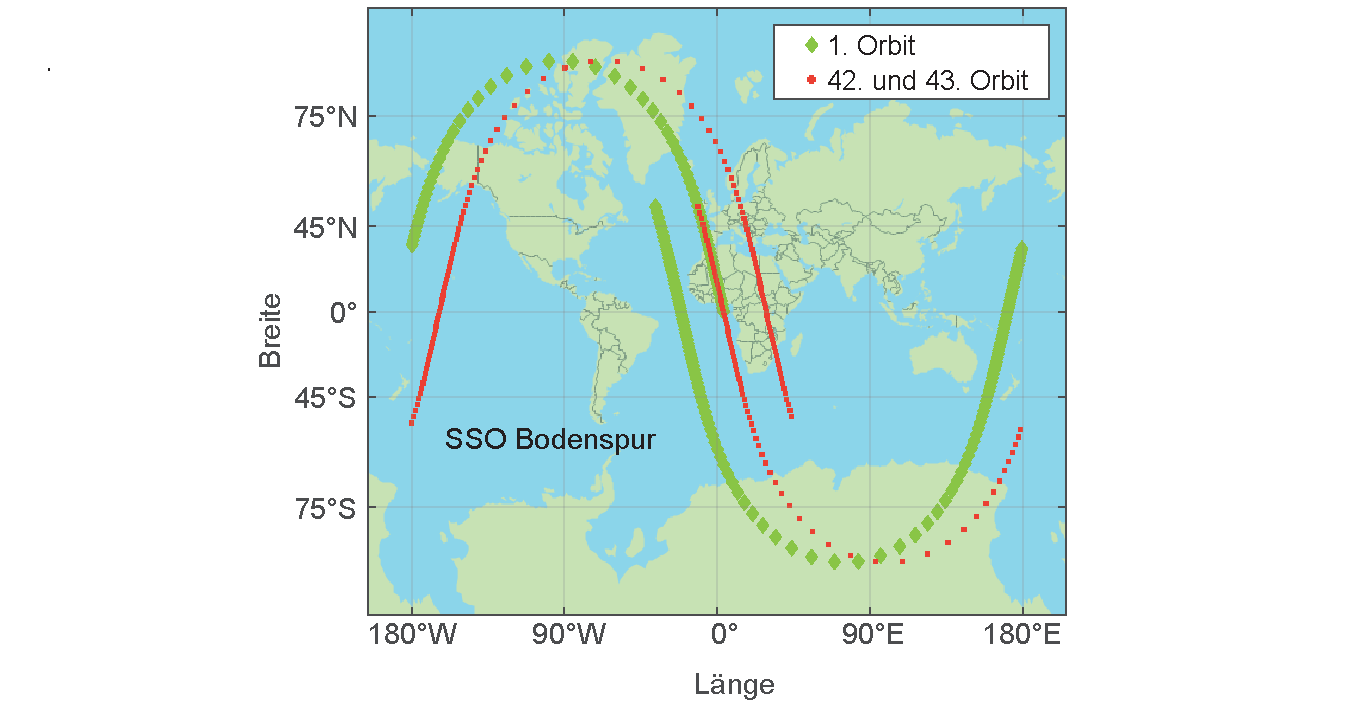
\includegraphics[width=\textwidth]{SonnensynchroneBodenspur.pdf} 
	\caption[Sonnensynchroner \textit{Repeat Orbit} -Bodenspur.]{Sonnensynchroner \textit{Repeat Orbit} - Bodenspur. Gezeigt sind Orbit Nr. 1 (willk�rlich gew�hlt) und die Orbits Nr 42 und Nr. 43 als Bodenspur. Man sieht, dass bei $N=43$ nach 3 Tagen der Satellit genau �ber die gleichen Gebiete fliegt wie beim Orbit $N=1$.}
	\label{abb:adyn_synchron_groundtrack}
\end{figure}

Wir empfehlen auch die Zusatz�bung \probref{adyn_pertubations}.

\end{sol} 
\textcolor{blue} {$\rightarrow$ zur} \probref{adyn_orbits5}.\\
\noindent\rule[1ex]{\textwidth}{0.5pt}  \newpage  \clearpage


%-----------------------------------------------------------------------------------------------------------

\begin{sol}{prob:adyn_starlink}\label{lsg:adyn_starlink} %�bung10
\textbf{Starlink}
\begin{figure}[H]
	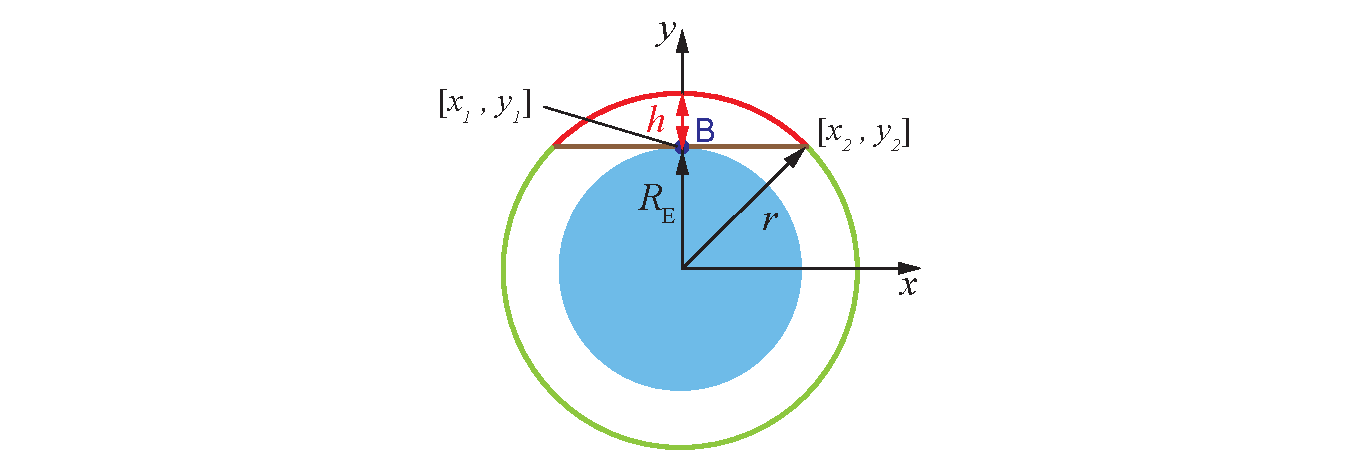
\includegraphics[width=\textwidth]{StarlinkGeometrie.pdf} 
	\caption[Zur Geometrie der Starlink-Beobachtungen.]{[Zur Geometrie der Starlink-Beobachtungen. Mit rot ist die Kugelkappe dargestellt die ein Beobachter auf der Erde sieht, wenn sich ein Starlink-Satellit in einer Kugelschale mit Radius $R_\text{E} + h$ bewegt.}
	\label{abb:adyn_starlink_ueb01}
\end{figure}
\begin{enumerate}
\item [1)] Wir berechnen zun�chst den Anteil $\gamma\lk h\rk$ der Kugelschale mit Radius $R_\text{E} + h$, den ein Beobachter von der Erdoberfl�che aus sieht. \\
    Nach \figref{adyn_starlink_ueb01} ist das:
    \begin{align*}
        \gamma\lk h\rk = \frac{A_\text{KK}}{A_\text{K}} \,. 
    \end{align*}
    Hierin ist $A_\text{K}$ ist die Oberfl�che einer Kugel $4\pi\,r^2 = 4\pi\,\lk R_\text{E} +h\rk^2$ und $A_\text{KK}$ die Oberfl�che der Kugelkappe, die man sich leicht �ber 
    \begin{align*}
       A_\text{KK} &= 2\pi\,r\int\limits_{x_1}^{x_2} y(x)\,\sqrt{1+y'(x){}^2}\D x = 2\pi\int\limits_{\rho_1}^{\rho_2} y(\rho)\,\sqrt{1+y'(\rho){}^2}\,\D \rho 
    \end{align*}
    mit $y = \sqrt{r^2-x^2}$,\,  $1+y'{}^2 = r^2/(r^2-x^2)$,\, $r = R_\text{E} + h$\, und \,$x= \rho\,\cos\phi$ herleiten kann.\\
		Somit erh�lt man 
    \begin{align}
		  A_\text{KK} &= 2\pi\,r \int\limits_{R_\text{E}}^{R_\text{E} + h}\,\D \rho = 2\pi\,\lk R_\text{E} +h\rk \,h \nonumber \\
      \rightarrow~~~  \gamma\lk h\rk &= \frac{2\pi\,\killA{\lk R_\text{E} + h\rk}\,h}{4\pi\,\lk R_\text{E} + h\rk^\killA{2}} = \frac{1}{2}\,\frac{h}{R_\text{E} + h} \,. \label{eq:adyn_starlink_ueb01}
    \end{align}
    Mit den Angaben aus der Aufgabenstellung sind damit jederzeit pro Schale $n_i $ Satelliten 
    \begin{align*}
        n_i = \gamma\lk n_i\rk \cdot \,N_i = 
        \begin{cases} 
        190 \\ 
        63\\
        223
        \end{cases}
    \end{align*}
    und insgesamt $n_\text{ges} = \sum n_i \approx 476$ Satelliten zu sehen.
\newpage
\item [2)] Wir nehmen eine Gleichverteilung der Satelliten in der Kugelschale an. Dann ergibt sich f�r einen Beobachter eine Raumwinkeldichte von
    \begin{align}
        \Omega_\text{ges} = \frac{n_\text{ges}}{2 \pi} \approx 75.8 \,. \label{eq:adyn_starlink_ueb03}
    \end{align}
    Der Nenner von $2\pi$ (anstelle $4\pi$) ergibt sich, aus der Tatsache, dass wir bereits in der Berechnung von \eqref{eq:adyn_starlink_ueb01} ber�cksichtigt hatten, dass der Beobachter nur den Halbraum sieht. Wir rechnen den Raumwinkel auf Quadratgrad ($\square^\degree$) um:
    \begin{align*}
        4\pi^2 = \lk 2\pi\rk^2 \widehat{=} \lk 360^\degree\rk^2 = 129600\,\square^\degree \,.
    \end{align*}
    und erhalten damit aus \eqref{eq:adyn_starlink_ueb03}
    \begin{align}
        \Omega_\text{ges} = \frac{n_\text{ges}}{2\pi} \approx 0.023\,\frac{1}{\square^\degree} \,.\label{eq:adyn_starlink_ueb04}
    \end{align}
    Umgekehrt hei�t das, dass f�r eine Kantenl�nge $d_\square$ eines Winkelquadrats am Himmel von 
    \begin{align}
        d_\square = \sqrt{A_\square} = \frac{1}{\sqrt{\Omega_\text{ges}}} \approx 6.6\degree   \label{eq:adyn_starlink_ueb05}
    \end{align}
    in etwa ein Starlink-Satellit zu sehen ist. \\
    Die Winkelgeschwindigkeit eines Starlink-Satelliten ist nach dem Keplerschen Gesetz durch
    \begin{align*}
        \omega_i = \sqrt{\frac{G\,M_\text{E}}{\lk R_\text{E} +h_i\rk^3}} = 
        \begin{cases} 
        \SI{3.95}{\degree\per\minute} \\ 
        \SI{3.75}{\degree\per\minute}\\
        \SI{3.3}{\degree\per\minute}
        \end{cases} \,.
    \end{align*}
    Der Mond hat einen Winkeldurchmesser von \ca $\SI{0.5}{\degree}$, \dh ein Starlink-Satellit \anf{durchquert} den Mond in weniger als $\Delta t = 0.5/\omega_i \approx \SI{8}{\second}$.
\end{enumerate}

\end{sol} 
\textcolor{blue} {$\rightarrow$ zur} \probref{adyn_orbits5}.\\
\noindent\rule[1ex]{\textwidth}{0.5pt}  \newpage  \clearpage





%-----------------------------------------------------------------------------------------------------------


\subsection{�bungen zu Man�vern im Weltall}

\medskip

%-----------------------------------------------------------------------------------------------------------

\begin{sol}{prob:adyn_rocket_analogy}\label{lsg:adyn_rocket_analogy} %�bung11
\textbf{Analogie zum Oberth-Effekt\index{Oberth-Effekt}}\\

Zun�chst k�nnte man denken, es spielt keine Rolle, wo die Rakete gez�ndet wird. Dem ist aber nicht so.\\
Wir betrachten den Gewinn an kinetischer Energie des Raketenautos durch den kurzen Raketenimpuls ($m_0$ ist die Masse der Rakete ohne Treibstoff) im festen KOS $\sum$:
\begin{align}
\begin{split}
    \Delta T_\text{R} &=\frac{1}{2}\,m_0\,\lk v+\Delta v\rk^2 - \frac{1}{2}\,m_0\,v^2\\
    &= \frac{1}{2}\,m_0\,\lk\Delta v\rk^2 - m_0\,v\,\Delta v  \,. 
\end{split}\label{eq:adyn_rocket_analogy01}
\end{align}
Der Gewinn an kinetischer Energie h�ngt interessanterweise von $v$ ab.\\
Der Impuls der gez�ndeten Rakete auf das Raketenauto ist aber unabh�ngig von $v$:
\begin{align}
    m_0\,\Delta v = m_\text{G}\,v_\text{G} = F\,\Delta t\,, \label{eq:adyn_rocket_analogy02}
\end{align}
worin $m_\text{G}$, $v_\text{G}$ die Masse \bzw die Geschwindigkeit des ausgesto�enen Treibgases sind, $F$ der Schub und $\Delta t$ ein kleines Zeitintervall. \\
Die Bezeichnung Ausstr�mgeschwindigkeit des Treibgases verdient eine genauere Betrachtung, es ist n�mlich die Geschwindigkeit des Gases relativ gemessen zum Schwerpunkt des Systems Raketenauto und Treibstoff. \\
Wie kann man das Paradoxon erkl�ren? Indem man die Ver�nderung der kinetischen Energie des Treibstoffs (\bzw der ausstr�menden Gase) wiederum im festen KOS $\sum$ betrachtet: 
\begin{align}
\begin{split}
    \Delta T_\text{G} &=\frac{1}{2}\,m_\text{G}\,\lk v_\text{G}-v\rk^2 - \frac{1}{2}\,m_\text{G}\,v^2\\
    &= \frac{1}{2}\,m_\text{G}\,v_\text{G}{}^2 - m_\text{G}\,v_\text{G}\,\Delta v \,.
\end{split} \label{eq:adyn_rocket_analogy03}
\end{align}
Man betrachte, dass hier in die Beziehung die Relativgeschwindigkeit $|v_\text{G} - v|$ eingeht, da im festen KOS sich ja der Treibstoff vor dem Z�nden bereits mit $v$ bewegt (\figref{adyn_rocket_analogy02}).\\

\begin{figure}[H]
	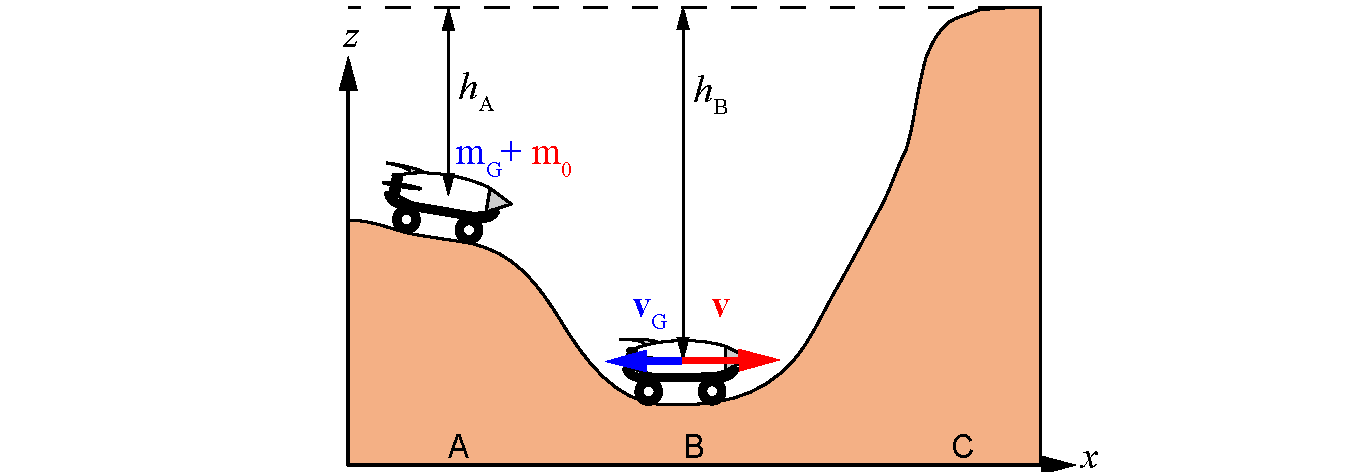
\includegraphics[width=\textwidth]{OberthEffAnalogie.pdf} 
	\caption[Analogie-Modell zum Oberth-Effekt.]{Analogie-Modell zum Oberth-Effekt.}
	\label{abb:adyn_rocket_analogy02}
\end{figure}

Die gesamte Ver�nderung der kinetischen Energie vom Raketenauto und Treibstoff muss gleich der freigesetzten chemischen Energie des Treibstoffs $\Delta E_\text{T}$ sein:
\begin{align}
\begin{split}
    \Delta T &= \Delta T_\text{R} + \Delta T_\text{G} \\
    &=\frac{1}{2}\,m_\text{G}\,v_\text{G}{}^2 + \frac{1}{2}\,m_0\lk\Delta v\rk^2 + \underbrace{m_0\,v\,\Delta v - m_\text{G}\,v\,v_\text{G}}_{\text{wegen \eqref{eq:adyn_rocket_analogy02}} =0} \\
    \Delta T &= \frac{1}{2}\,m_\text{G}\,v_\text{G}{}^2 + \frac{1}{2}\,m_0\lk\Delta v\rk^2 = \Delta E_\text{T}\,. 
\end{split} \label{eq:adyn_rocket_analogy04}
\end{align}
Die gesamte kinetische Energie ist wie erwartet unabh�ngig von $v$ und wegen der Energieerhaltung gleich $\Delta E_\text{T}$. \\

Was bedeutet das nun f�r den Z�ndungszeitpunkt? Wir untersuchen zwei Zeitpunkte (\bzw Orte) $A$ und $B$. 
Es gilt f�r die Gesamtenergien vor dem Z�nden:
\begin{align*}
    E_\text{A} &= -\lk m_0+ m_\text{G}\rk\,g\,h_\text{A}  \,,\\
    E_\text{B} &= -\lk m_0 + m_\text{G} \rk\,g\,h_\text{B} + T_\text{B} \\
    &= -\lk m_0+m_\text{G}\rk\,g\,h_\text{B}  + \frac{1}{2}\lk m_\text{G} +m_0\rk\,v_\text{B}{}^2 = -\lk m_0 + m_\text{G} \rk\,g\,h_\text{A}     \,.
\end{align*}
Aus $E_\text{A} = E_\text{B}$ folgt $v_\text{B} = \sqrt{2g\lk h_\text{B} -h_\text{A}\rk }$.\\

Unmittelbar nach dem Z�nden am Punkt $B$ gilt:
\begin{align*}
    E_\text{R}' =\,&\frac{1}{2}\,m_0\lk v_\text{B}+\Delta v\rk^2 - m_0\,g\,h_\text{B} + \frac{1}{2}\,m_\text{G}\lk v_\text{B} -v_\text{G}\rk^2 - m_\text{G}\,g\,h_\text{B}\\
    = \,&\frac{1}{2}\,m_0\lk\Delta v\rk^2 + m_0\,g\,h_\text{A} -m_0\,\Delta v\,\sqrt{2g\lk h_\text{B}-h_\text{A}\rk} \,,\\
		E_\text{G}' = \,& \frac{1}{2}\,m_\text{G}\,v_\text{G}{}^2 -m_\text{G}\,g\,h_\text{A} - m_\text{G}\,v_\text{G}\,\sqrt{2g\lk h_\text{B}-h_\text{A}\rk} \,,\\
    E_\text{ges}' = \,&\frac{1}{2}\,m_0\,\lk\Delta v\rk^2 + \frac{1}{2}\,m_\text{G}\,v_\text{G}{}^2 - \lk m_0 + m_\text{G}\rk\,g\,h_\text{A} = \, E_\text{A} + \Delta E_\text{T} \,.
\end{align*}
Man erkennt, dass die Energie der Rakete einen von $\sqrt{\lk h_\text{B} -h_\text{A}\rk}$ abh�ngigen Term hat, der offensichtlich verschwindet, wenn $h_\text{B} = h_\text{A}$ ist, es also keine Potentialmulde gibt. \\
Wir bestimmen jetzt noch wie gro� $\Delta v$ sein mu�, um den Punkt C zu erreichen, wenn die Rakete bei $B$ gez�ndet wird. 
\begin{align}
\begin{split}
    \frac{1}{2}\,m_0\,v_\text{C}{}^2 &= \frac{1}{2}\,m_0\,\lk \Delta v\rk^2 - m_0\,g\,h_\text{A} +m_0\,\Delta v \,\sqrt{2g\lk h_\text{B}-h_\text{A}\rk}\\
    \rightarrow ~~~~ 0 &= \lk \Delta v\rk^2 + 2\,\Delta v\,\sqrt{2g\lk h_\text{B}-h_\text{A}\rk} - 2\,g\,h_\text{A}\\
    \rightarrow ~~~~ \lk \Delta v\rk_\text{min} &= \sqrt{2g\lk h_\text{B}-h_\text{A}\rk} + \sqrt{\frac{g}{2}\,\lk h_\text{B}-h_\text{A}\rk + 2\,g\,h_\text{A}} 
\end{split}\,.\label{eq:adyn_rocket_analogy06}
\end{align}
Wie erwartet wird $\Delta v$ f�r $h_\text{B} = h_\text{A}$ zu $\Delta v= \sqrt{2\,g\,h_\text{A}}$. \\
Wir haben $\Delta v\lk h_\text{B}, h_\text{A}\rk$ in \figref{adyn_rocket_analogy03} dargestellt.\\

Die Analogie zum Oberth-Effekt der Raumfahrt ist offensichtlich. Wenn man den gr��tm�glichen beschleunigenden Effekt auf ein Raumschiff haben will, startet man das Man�ver am Punkt der Bahn, wo die Geschwindigkeit am gr��ten ist, \dh im Perig�um oder allgemein an der Periapsis. \\
Einfach gesprochen besagt der Oberth-Effekt, dass ein Raumschiff bei einem Impulsman�ver etwas Energie zus�tzlich zur chemischen Energie des Treibstoffs  \anf{stehlen} kann und zwar von der urspr�nglichen kinetischen Energie, die der Treibstoff vor dem Z�nden auf Grund der Bewegung der Rakete hatte. Anders gesagt: Der Schub generiert einen Impuls proportional zu $\Delta v$. Da die Energie proportional zu $v^2$ ist, ist dieser generierte Impuls energetisch um so wirksamer, je gr��er die Geschwindigkeit $v$ zu Beginn des Schubs ist.


\begin{figure}[H]
	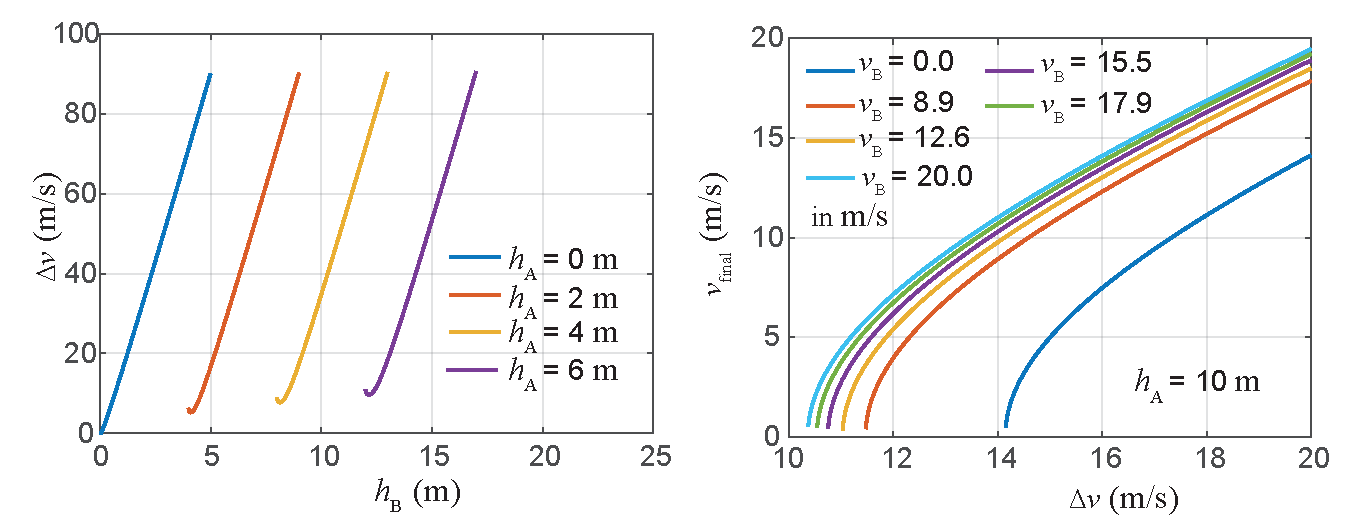
\includegraphics[width=\textwidth]{OberthEffAnalogie02.pdf} 
	\caption[Antriebsbedarf eines Raketenautos durch eine Potentialmulde.]{Antriebsbedarf eines Raketenautos durch eine Potentialmulde als Analogie-Modell zum Oberth-Effekt (Parameter siehe \mscr~\mladynref{OberthEffektAnalogie.m}).}
	\label{abb:adyn_rocket_analogy03}
\end{figure}

\end{sol} 
\textcolor{blue} {$\rightarrow$ zur} \probref{adyn_rocket_analogy}.\\
\noindent\rule[1ex]{\textwidth}{0.5pt}  \newpage  \clearpage


%-----------------------------------------------------------------------------------------------------------

\begin{sol}{prob:adyn_manoevers1}\label{lsg:adyn_manoevers1} %�bung12
\textbf{Hohmann-Transfer}
\begin{itemize}
   \item �bergangszeit f�r den Hohmann-Transfer als Funktion von $r_2/r_1$ \\
	Die �bergangszeit ergibt sich als halbe Umlaufzeit f�r die Hohmann-Ellipse:
	\begin{align*}
    t_\text{H} = \pi\sqrt{\frac{a_\text{H}{}^3}{m_\text{ZK}\,G}} = \frac{\pi}{\sqrt{m_\text{ZK}\,G}}\,\sqrt{\lk \frac{r_1+r_2}{2}\rk^3}\,.
\end{align*}
F�r den Fall eines Hohmann-Transfers von der Erdbahn in den interplanetaren Raum sind die Zeiten in \figref{adyn_Hohmann_TOF} dargestellt (\mscr~\mladynref{HohmannTransfer.m}).
\begin{figure}[H]
	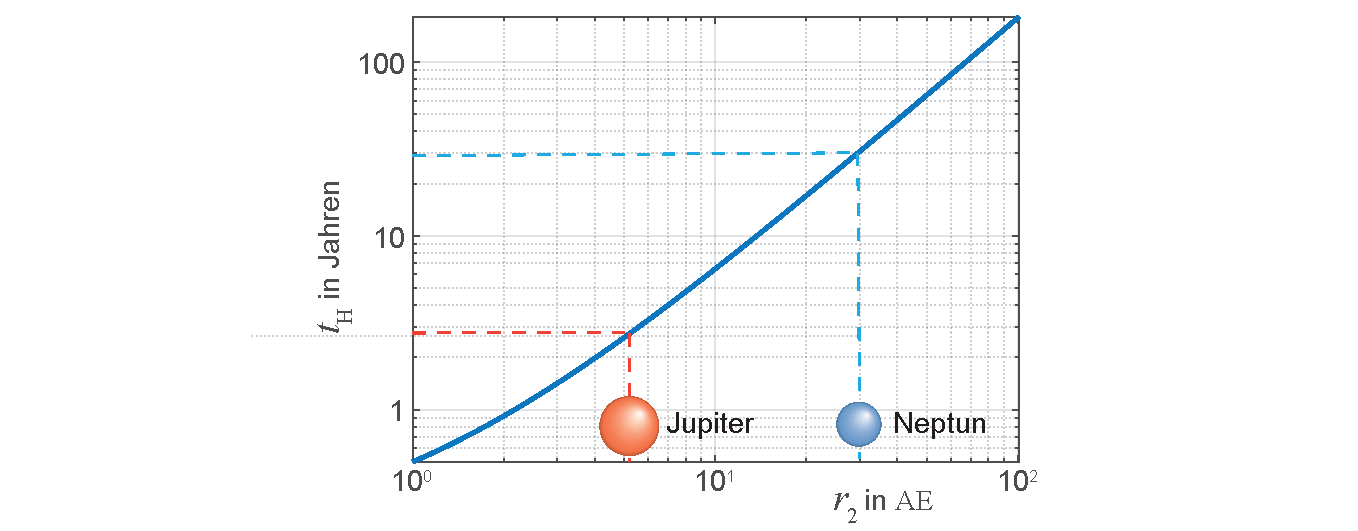
\includegraphics[width=\textwidth]{HohmannTOF.pdf} 
	\caption[Hohmann-Transferzeiten.]{Hohmann-Transferzeiten.}
	\label{abb:adyn_Hohmann_TOF}
\end{figure}
   \item $\Delta v$ gr��er als die \gls{vescape}\\
	F�r $r_2 \rightarrow \infty$ geht $\Delta v_2 \rightarrow 0$ und $\Delta v_1 \rightarrow v_\text{F}$. Daher ist in einem Bereich von $3.3 < r_2/r_1 < \infty$ die Summe $\Delta v_1+\Delta v_2$ gr��er als $v_\text{F}$, wie man leicht aus \eqref{eq:adyn_hohmann04} zusammen mit \eqref{eq:adyn_hohmann03a} und  \eqref{eq:adyn_hohmann03b} herleiten kann.\\
	Im Allgemeinen braucht man insgesamt mehr Antriebsenergie wenn eine Raumsonde erst impulsiv beschleunigt wird, dann durch Gravitation verlangsamt wird und anschlie�end wieder beschleunigt wird, als wenn die gesamte Antriebsimpuls in der Form von $\Delta v_1 = v_\text{F}$ aufgebracht wird.\\
   \item Hohmann-Transfer f�r Verringerung des Bahnradius\\
	Beim Hohmann-�bergang von h�heren auf niedrigere Bahnen gelten die Formeln unver�ndert, der Antriebsbedarf ist negativ und als Schub gegen die Flugrichtung zu verstehen.\\
\end{itemize}

\end{sol} 
\textcolor{blue} {$\rightarrow$ zur} \probref{adyn_manoevers1}.\\
\noindent\rule[1ex]{\textwidth}{0.5pt}  \newpage  \clearpage

%-----------------------------------------------------------------------------------------------------------
\begin{sol}{prob:adyn_manoevers2}\label{lsg:adyn_manoevers2} %�bung13
\textbf{Bielliptischer �bergang}\\

Zwei-Impuls-�bergang von Bahn mit Radius $r_1$ auf eine elliptische Bahn mit Radius $r_2$: 
F�r den Hohmann-Transfer nach $\infty$ ($r_2 \to\infty)$ k�nnen wir schreiben:
\begin{align*}
    \Delta v_1 = \sqrt{\frac{\mu}{r_1}}\,\lk \sqrt{2}-1\rk = v_1\lk \sqrt{2}-1\rk\,.
\end{align*}
Hierin ist $\mu$ der Gravitationsparameter f�r den jeweiligen betrachteten Zentrlk�rper (Erde, Sonne). Analog folgt in der umgekehrten Richtung (aus dem $\infty$ auf die Kreisbahn $r_2$):
\begin{align*}
    \Delta v_2 = v_2 \lk \sqrt{2}-1 \rk
\end{align*}
und somit mit $ \gamma = r_2 / r_1$:
\begin{align*}
    \frac{\Delta v_2}{v_1} = \frac{v_2}{v_1}\,\lk \sqrt{2}-1\rk = \sqrt{\frac{r_1}{r_2}} \,\lk\sqrt{2}-1\rk = \frac{\sqrt{2}-1}{\sqrt{\gamma}}\,.
\end{align*}
Der Gesamt-Antriebsbedarf ist dann: 
\begin{align*}
    \frac{\Delta v}{v_1} = \frac{\Delta v_1+\Delta v_2}{v_1} = \frac{\Delta v_1}{v_1}+\frac{\Delta v_2}{v_1} = \lk \sqrt{2} -1\rk\lk 1 + \frac{1}{\sqrt{\gamma}}\rk\,.
\end{align*}
\begin{figure}[H]
	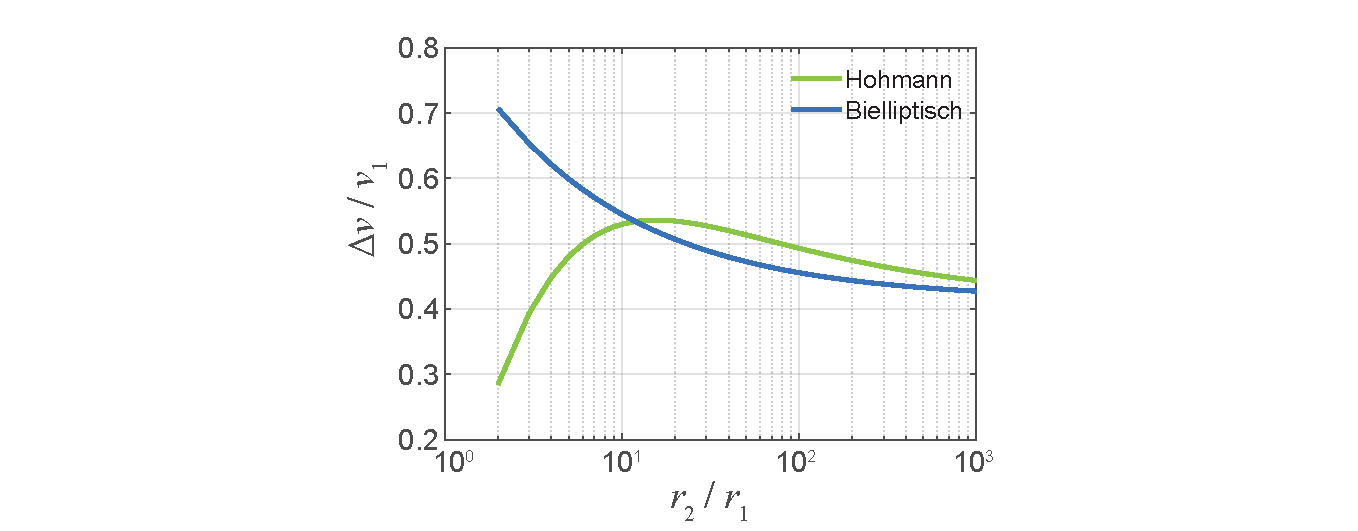
\includegraphics[width=\textwidth]{BiEllptischerTransfer.pdf} 
	\caption[Bielliptischer Transfer.]{Antriebsbedarf beim bielliptischen Transfer im Vergleich zum Hohmann-Transfer.}
	\label{abb:adyn_manoevers2}
\end{figure}

Man erkennt aus \figref{adyn_manoevers2}, dass in der Tat f�r gro�e Radienverh�ltnisse ($\gamma > \SI{11.94}{}$) der bielliptische-Transfer energetisch g�nstiger ist.\\
Allerdings erkauft man sich das durch sehr lange Transferzeiten. Vorteilhaft sind solche bielliptischen �berg�nge aber, wenn man die Inklination und Umlaufrichtung des Orbits �ndern will. Die Rechnungen sind im Detail im \mscr~\mladynref{BiElliptischerTransfer.m} ausgef�hrt.
Die in der Abbildung gezeigten Trajektorien der hyperbolischen Bahnen sind nach \kap{hm_bewegungsgl} gegeben durch:
\begin{align}
	 r = \frac{a\,\lk 1 - e^2 \rk}{1 - e\,\cos\upsilon} ~~~\text{mit}~~~\upsilon < \arccos\frac{1}{e} ~~~\text{und}~~~a = \frac{r_\text{P}}{(1-e)} \,.	\label{eq:adyn_oberth37}
\end{align}
Die geometrischen Parameter $a$ und $e$ der Hyperbel sind durch die physikalischen Parameter $H$ \bzw $v_\infty$ und $r_\text{P}$ definiert (vgl. \kap{hm_bewegungsgl}: $~a < 0,\, e > 1$):
\begin{align}
	 a = -\frac{\mu}{2H_\infty} = -\frac{\mu}{v_\infty{}^2} ~~~\text{und}~~~e = 1 + \frac{r_\text{P}\,v_\infty{}^2}{\mu} \,.	\label{eq:adyn_oberth38}
\end{align}

\end{sol} 
\textcolor{blue} {$\rightarrow$ zur} \probref{adyn_manoevers2}.\\
\noindent\rule[1ex]{\textwidth}{0.5pt}  \newpage  \clearpage

%-----------------------------------------------------------------------------------------------------------

\begin{sol}{prob:adyn_manoevers3}\label{lsg:adyn_manoevers3} %�bung14
\textbf{Hohmann-Oberth-Edelbaum-Transfers aus dem Orbit nach $\infty$}\\

Die Rechnungen sind explizit im \mscr~\mladynref{TransferUnendlich.m} hinterlegt und die Ergebnisse in \figref{adyn_Oberth_transfer2} und \figref{adyn_Oberth_transfer3} gezeigt. 
Man erkennt, dass es f�r gr��ere finale Abst�nde $r_\text{end}$ und bestimmte Verh�ltnisse von $r_{+}/r_1$  ein Minimum der Flugzeit f�r den Edelbaum-Transfer gibt. Er ist in den meisten F�llen der energetisch g�nstigste Transfer. Der Hohmann-Transfer ist f�r gro�e Entfernungen sowohl was die Flugzeit als auch den Antriebsbedarf betrifft der ung�nstigste.\\

\begin{figure}
	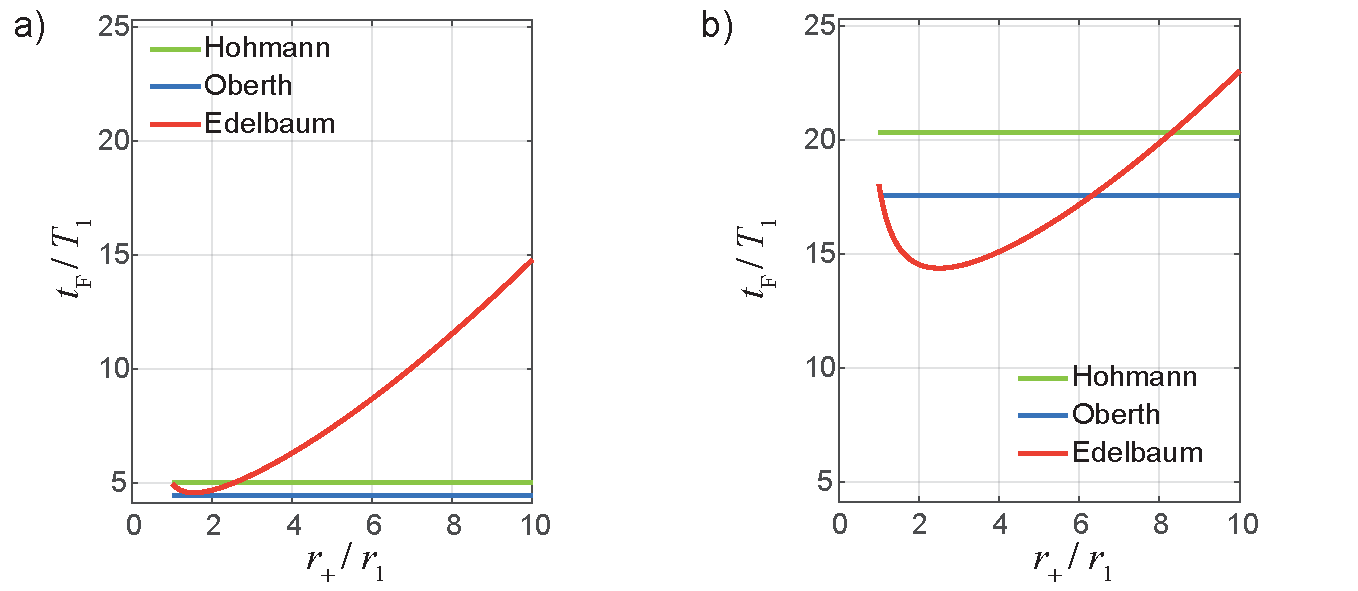
\includegraphics[width=\textwidth]{TransfersInfin03.pdf} 
	\caption[Flugzeiten beim Transfer nach $\infty$.]{Flugzeiten beim Hohmann-, Oberth- \bzw Edelbaum-Transfer. \fa bis zu $r_\text{end}=50\,r_1$ \fb bis zu $r_\text{end}=200\,r_1$.  Als variabler Parameter wurde der �u�ere Radius $r_{+}$ genommen, der innere Radius wurde als fix mit $r_{-}=0.05\,r_1$ gesetzt und der Schubparameter wurde mit $\Delta v/v1 = 1.1$ angenommen. Man erkennt, dass es f�r $r_{+}\approx 2.5\,r_1$ ein absolutes Minimum der Flugzeit f�r den Edelbaum-Transfer gibt. Danach f�hrt die l�ngere Flugzeit auf der Halbellipse von $r_{+}$ nach $r_{-}$ zu insgesamt l�ngeren Flugzeiten.} \label{abb:adyn_Oberth_transfer3}
\end{figure}

\end{sol} 
\textcolor{blue} {$\rightarrow$ zur} \probref{adyn_manoevers3}.\\
\noindent\rule[1ex]{\textwidth}{0.5pt}  \newpage  \clearpage

%-----------------------------------------------------------------------------------------------------------

\begin{sol}{prob:adyn_manoevers4}\label{lsg:adyn_manoevers4} %�bung15
\textbf{Lambert-Problem}\\

Die allgemeine Formulierung des Lambert-Problems lautet wie folgt (\figref{adyn_lambert_lsg02a}):\\
Es seien zwei Punkte $\text{P}_1,\, \text{P}_1$ im Raum durch ihre Vektoren $\vec{r}_1$, $\vec{r}_2$ bekannt, ebenso die Zeit $t_\text{F} = t_2-t_1$, die f�r die Bewegung des K�rpers zwischen $\mathrm{P}_1$ und $\mathrm{P}_2$ ben�tigt wird. Gesucht sind f�r die Kepler-Ellipse die Bahnparameter $a$, $e$, $ \upsilon_0$.\footnote{Wir wollen hier nur Ellipsenbahnen betrachten. Man kann das Problem auch f�r Hyperbelbahnen formulieren und l�sen, siehe \ua \cite{Izzo2015, Walter2018}. Im wesentlichen werden dabei die Winkelfunktionen durch die Hyperbelfunktionen ersetzt.}\\

\begin{figure}[H]
	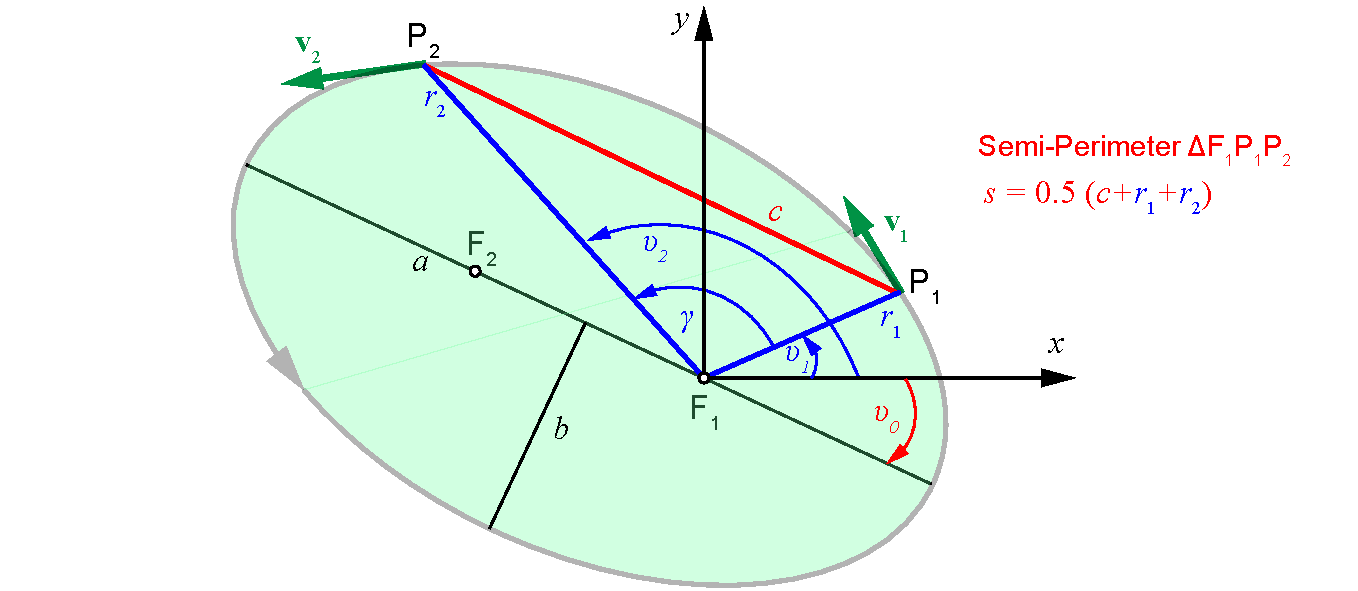
\includegraphics[width=\textwidth]{LambertProblem02Geometrie.pdf} 
	\caption[Geometrie des Lambert-Problems.]{Geometrie des Lambert-Problems. Parameter siehe Text.}
	\label{abb:adyn_lambert_lsg02a}
\end{figure}

Zun�chst schreiben wir die Kepler-Gleichung f�r die beiden Zeitpunkte auf ($\mu$ ist hierin der Gravitationsparameter des Zentralk�rpers, in dessen Schwerefeld die Bewegung stattfindet.) und subtrahieren die beiden Gleichungen voneinander. Wir erhalten:
\begin{align}
\sqrt{\frac{\mu}{a^3}}\,\lk t_2-t_1\rk &= \sqrt{\frac{\mu}{a^3}}\,t_\text{F} = E\lk t_2\rk - E\lk t_1\rk -e\,\lek \sin E\lk t_2\rk -\sin E\lk t_1\rk\rek \nonumber \\
\rightarrow ~~~~ \sqrt{\frac{\mu}{a^3}} \,t_\text{F} &= E_2-E_1 -e\,\lk \sin E_2 -\sin E_1\rk \label{eq:adyn_lsglambert01}\,.
\end{align}
Durch die Randwerte ist ja ein Brennpunkt der Ellipse, n�mlich $\mathrm{F}_1$ bekannt. Man sucht nun den Brennpunkt $\mathrm{F}_2$ (oft auch versteckter Fokus genannt), mit dem dann die Ellipse eindeutig definiert ist und zugleich die Bedingung erf�llt ist, dass f�r das Durchlaufen von $\mathrm{P}_1$ nach $\mathrm{P}_2$ die Zeit $t_\text{F}$, im Englischen auch \gls{ToF} (ToF), ben�tigt wird. 

\begin{figure}[H]
	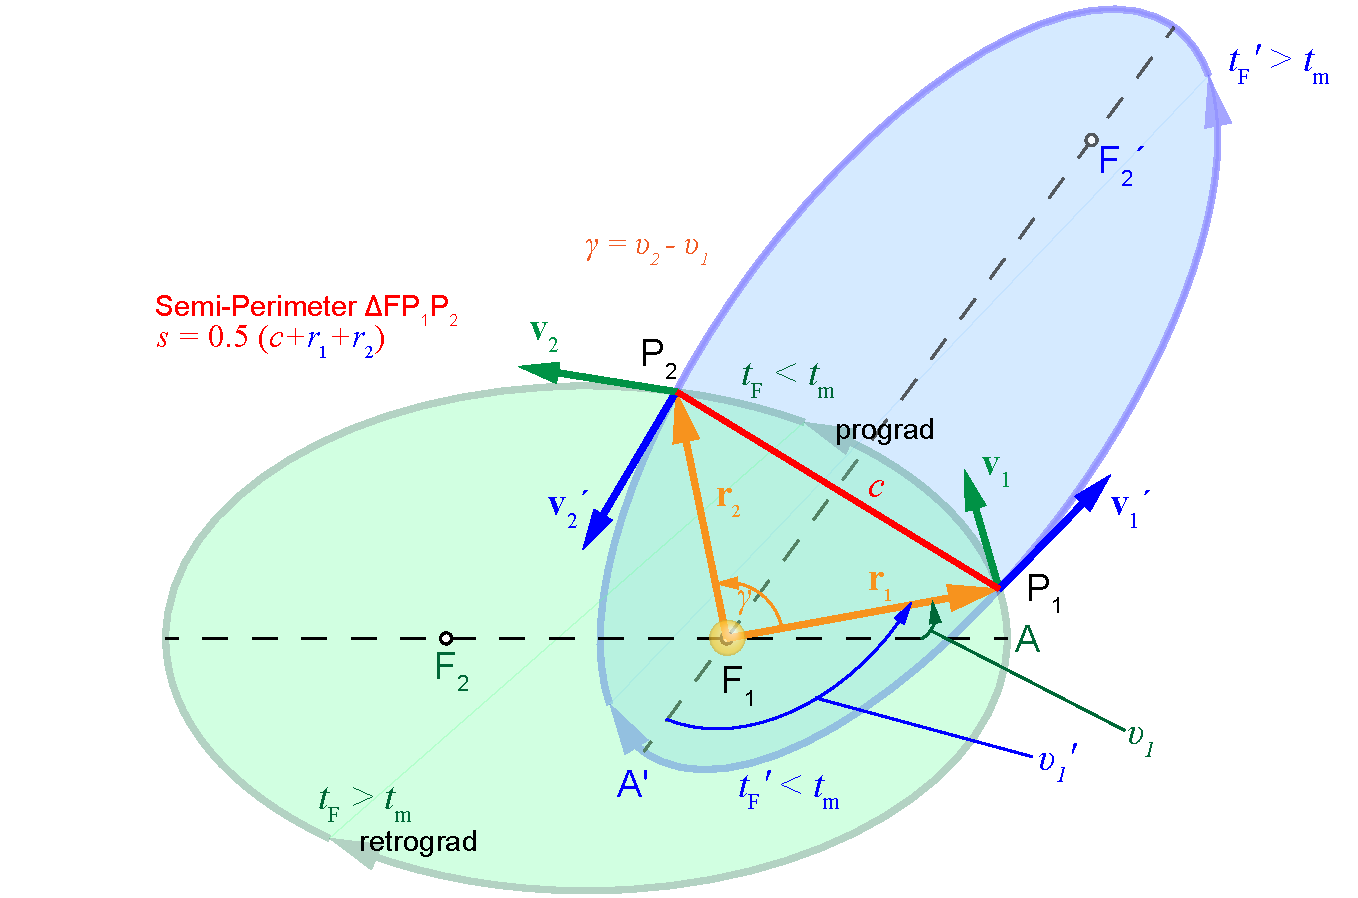
\includegraphics[width=\textwidth]{LambertProblem02Allgemein.pdf} 
	\caption[Geometrie des Lambert-Problems.]{Geometrie des Lambert-Problems. Die beiden Ellipsen (gr�n und blau schattiert) stellen jeweils eine L�sung des Lambert-Problems f�r unterschiedliche Flugzeiten und Flugrichtungen dar. Die Flugrichtung wird als prograd bezeichnet, wenn diese entgegen des Uhrzeigersinns von $\mathrm{P}_1$ nach $\mathrm{P}_2$ erfolgt, die entgegengesetzte Flugrichtung wird retrograd genannt. Die Vektoren $\vec{r}_1$, $\vec{r}_2$ definieren die Ellipsen, sie k�nnen als Positionsvektoren aber auch zu unterschiedlichen Umlaufbahnen geh�ren, \zb $\vec{r}_1$ kann ein Vektor von der Sonne zur Erde sein, $\vec{r}_2$ eine entsprechender Vektor zum Mars. Weitere Parameter siehe Text.}
	\label{abb:adyn_lambert_lsg02}
\end{figure}
Wir k�nnen uns nun leicht �berlegen, dass es f�r die gesuchte Bahn zwei Ellipsen als denkbare L�sungen gibt und zwar mit den beiden "`versteckten"' Fokuspunkten $\mathrm{F}_2$ und $\mathrm{F}_2{}'$ (\figref{adyn_lambert_lsg02})\footnote{Man kann sich die zwei L�sungen anschaulich-geometrisch deutlich machen, in dem man sich die Konstruktionsvorschrift einer Ellipse in Erinnerung ruft. Nach dieser ist an jedem Punkt einer Ellipse die Summe des Abstandes zu den beiden Fokuspunkten konstant und gleich $2a$. Die Konstruktion erfolgt, in dem man einen Kreis um $\mathrm{P}_1$ mit dem Radius $2a-r_1$ schl�gt und einen um $\mathrm{P}_2$ mit $2a-r_2$. Es ergeben sich zwei Schnittpunkte, dies sind die Brennpunkte $\mathrm{F}_2$ \bzw $\mathrm{F}_2{}'$.}.\\
Mit den Beziehung \eqref{eq:hm_r_param_ellipse} und \eqref{eq:hm_bahnglg} aus dem \kap{hm_abl_kepler} k�nnen wir schreiben: 
\begin{subequations}
\begin{align}
    r_{1,2} &= a\,\lk 1-e\,\cos E_{1,2}\rk  \label{eq:adyn_lsglambert02a} \,,\\
    \cos\lk \upsilon_{1,2}-\upsilon_0\rk &= \frac{a}{r_{1,2}}\,\lk\cos E_{1,2}-e\rk \,. \label{eq:adyn_lsglambert02b}
    %r_{1,2}\cos{\upsilon_{1,2}} &= a\,\lk \cos E_{1,2} - e \rk \,, \label{eq:adyn_lsglambert02b} \\
    %r_{1,2}\sin{\upsilon_{1,2}} &= a\,\sqrt{\lk 1-e^2 \rk}\, \sin E_{1,2} \,, \label{eq:adyn_lsglambert02c} \\
\end{align} %\label{eq:adyn_lsglambert02} 
\end{subequations}
Wir betrachten eine der beiden Ellipsen aus \figref{adyn_lambert_lsg02} genauer und verwenden die Darstellung in \figref{adyn_lambert_lsg02a}. Unser Ziel ist es ja, die Trajektorie $r(\upsilon)$ zu finden:
\begin{align}
    r (\upsilon) &= \frac{a\,\lk 1 - e^2 \rk}{1+e\,\cos\lk\upsilon - \upsilon_0 \rk}\,. \label{eq:adyn_lsglambert_traj} 
\end{align} 
In einer Ebene ist eine Trajektorie (Bahn) durch 3 Parameter eindeutig bestimmt. Das Lambert-Problem ist ein planares Problem und wir
haben mit dem Gleichungssystem \eqref{eq:adyn_lsglambert01}, \eqref{eq:adyn_lsglambert02a} und \eqref{eq:adyn_lsglambert02b} ein System f�r 5 Unbekannte $E_1$, $E_2$, $a$, $e$, $\upsilon_0$ mit den bekannten Gr��en $r_1$, $r_2$, $\upsilon_1$, $\upsilon_2$, $t_\text{F}$ und $\mu$.\footnote{Eigentlich sind $\upsilon_1$, $\upsilon_2$ ja nicht bekannt, sondern nur deren Differenz. Durch freie Festlegung eines \KOS wie in \figref{adyn_lambert_lsg02a} gezeigt kann man sich aber $\upsilon_1$ und $\upsilon_2$ berechnen. Man beachte, dass dieses \KOS mit den $x-y$- Achsen in der Ellipsenebene liegt und gegebenenfalls durch Drehung in ein anderes (\zb heliozentrisches) \KOS transformiert werden muss, wenn man die koordinaten der Trajektorie in diesem haben  m�chte.} Dieses System wollen wir jetzt l�sen:
\begin{enumerate}
    \item [1.] Mit der Nebenrechnung (\cite{Gradshteyn1980})
		\begin{align*}
		\sin x - \sin y =&  \sin{\lk \frac{x-y}{2} +  \frac{x+y}{2}\rk} - \sin{\lk \frac{x+y}{2} +  \frac{-x+y}{2}\rk} \\
		=& \sin{\lk \frac{x-y}{2} +  \frac{x+y}{2}\rk} + \sin{\lk \frac{x-y}{2} + \frac{-x-y}{2} \rk} \\
		=& \sin\lk \frac{x-y}{2}\rk\,\cos\lk\frac{x+y}{2}\rk + \sin\lk \frac{x+y}{2}\rk\,\cos\lk\frac{x-y}{2}\rk\\
		&+ \sin\lk \frac{x-y}{2}\rk\,\cos\lk\frac{x+y}{2}\rk - \sin\lk \frac{x+y}{2}\rk\,\cos\lk\frac{x-y}{2}\rk \\
		=& 2\,\sin{\frac{x-y}{2}}\,\cos{\frac{x+y}{2}}
		\end{align*}
    f�hren wir $\psi$ und $\varphi$ als neue Variable ein:
    \begin{align}
        \psi = \frac{E_2-E_1}{2}~~~~ \text{und} ~~~~ \cos \varphi = e\,\cos\lk \frac{E_2 +E_1}{2} \rk \,, \label{eq:adyn_lsglambert06}
    \end{align}
		wobei $\psi \in [0, \pi]$ und $\varphi \in [0, \pi]$ gilt. Wir erhalten dann die Kepler-Gleichung \eqref{eq:adyn_lsglambert01} in folgender vereinfachter Form:
\begin{align}
			\sqrt{\frac{\mu}{a^3}} \,t_\text{F} &= \psi - \cos\varphi\, \sin\psi \label{eq:adyn_lsglambert01a}\,.
\end{align}
Die beiden Gr��en $\psi$ und $\varphi$ h�ngen nur von der vorgegebenen Geometrie des Problems ab, wie man leicht nachrechnen kann, in dem man 
den Abstand von $\mathrm{P}_1$ und $\mathrm{P}_2$ unter Verwendung von \eqref{eq:adyn_lsglambert02b} �ber 
    \begin{align}
        c^2 &= \lk r_2\,\cos\upsilon_2 - r_1\,\cos\upsilon_1 \rk^2 + \lk r_2\,\sin\upsilon_2 - r_1\,\sin\upsilon_1 \rk^2 ~\nonumber \\
				&= r_1{}^2+r_2{}^2 - 2\,r_1\,r_2\,\cos\lk \upsilon_2-\upsilon_1\rk = r_1{}^2+r_2{}^2 - 2\,r_1\,r_2\,\cos\lk \gamma \rk~\nonumber \\
				\rightarrow~~c &= 2 a\,\sin\psi\,\sin\varphi\, \label{eq:adyn_lsglambert03a}
    \end{align}
berechnet. 
Ebenso erh�lt man die Summe der Abst�nde $r_1+r_2$ von den Punkten $\mathrm{P}_1$ und $\mathrm{P}_2$ zum Brennpunkt $\mathrm{F}_1$ wiederum unter Verwendung von \eqref{eq:adyn_lsglambert02b} zu
		\begin{align}
		r_1 + r_2  &= 2a\lk 1- \cos\psi\, \cos\varphi \rk\,. \label{eq:adyn_lsglambert03b}
    \end{align} 
Die Gleichungen \eqref{eq:adyn_lsglambert03a} und \eqref{eq:adyn_lsglambert03b} bestimmen die Gr��en $\psi$ und $\varphi$ eindeutig. Man kann also schlussfolgern, dass die Zeit $t_\text{F}$ nach \eqref{eq:adyn_lsglambert01a} nur eine Funktion von $a$ und den bekannten geometrischen Gr��en $c$ und $r_1 + r_2$  ist.\footnote{Der Beweis daf�r wurde von Lagrange erbracht, der zeigte, dass die ToF $t_\text{F}$ nur von der Energie der Bahn und damit nur von $a$ abh�ngt.}\\   

\item [2.] Um uns die Rechnungen zu erleichtern, f�hren wir zwei weitere Gr��en ein, die wir aus $\varphi$ und $\psi$ wie folgt bilden:
				\begin{align}
						\alpha= \varphi +\psi ~~~~ \text{und} ~~~~ \beta= \varphi-\psi \,. \label{eq:adyn_lsglambert05}
				\end{align}
		Offensichtlich gilt: $\alpha \in [0,\, 2\pi]$ und $\beta \in [-\pi,\, \pi]$. \\
		
\item [3.] Wir bezeichnen den halben Umfang (Semi-Perimeter) des Dreiecks $\Delta \,\mathrm{F}_1\mathrm{P}_1\mathrm{P}_2$ mit 
    \begin{align}
        s= \frac{r_1+r_2+c}{2}\,. \label{eq:adyn_lsglambert04}
    \end{align}
		Damit und mit \eqref{eq:adyn_lsglambert03a} und \eqref{eq:adyn_lsglambert03b} findet man  f�r $\alpha$ die Beziehung: 
    \begin{subequations}
    \begin{align}
        \frac{s}{2a} &= \frac{1}{2} \lek 1 - \cos\psi\cos\varphi + \sin\psi\sin\varphi \rek = \frac{1}{2} \lek 1 - \cos \lk \psi+\varphi \rk \rek \nonumber \\
				&= \frac{1}{2} \lek 1 - \cos\alpha \rek = \frac{1}{2} \lek 1 - \cos\lk \frac{\alpha}{2} + \frac{\alpha}{2} \rk \rek \nonumber \\
				&= \frac{1}{2} \lek 1 - \cos^2\frac{\alpha}{2} + \sin^2\frac{\alpha}{2} \rek = \frac{1}{2} \lek 2\sin^2\frac{\alpha}{2} \rek \nonumber \\
        &\rightarrow~~ \sin^2\lk \frac{\alpha}{2}\rk = \frac{s}{2a}\, \label{eq:adyn_lsglambert06a} \\
				&\text{und entsprechend f�r}~~ \beta \nonumber \\
        &\rightarrow~~ \sin^2\lk\frac{\beta}{2}\rk = \frac{s-c}{2a}\,\label{eq:adyn_lsglambert06b}
    \end{align}
    \end{subequations}
    Sowohl $\alpha$ als auch $\beta$ sind somit Gr��en, die nur von der Geometrie der Aufgabenstellung und dem Bahnparameter $a$ abh�ngen.\\
		
\item [4.] Wir setzen nun \eqref{eq:adyn_lsglambert06a} und \eqref{eq:adyn_lsglambert06b} in \eqref{eq:adyn_lsglambert01} ein und erhalten die elegante Formulierung des Lambert-Problems 
\begin{align}
    t_\text{F} &= \sqrt{\frac{a^3}{\mu}}\,\lk \alpha-\beta-\lek\sin\alpha -\sin\beta\rek\rk\,,\label{eq:adyn_lsglambert07}
\end{align}   
Damit haben wir $E_2$, $E_1$ aus der Kepler-Gleichung eliminiert und das Lambert-Problem auf ein System von 3 Unbekannten ($a$, $\alpha$, $\beta$) zur�ck gef�hrt, von den $\alpha$ und $\beta$ neben den bekannten Gr��en $s$, $c$ nur noch von $a$ abh�ngen. Der Winkel $\alpha$ ist dabei wegen des Quadrats in \eqref{eq:adyn_lsglambert06a} nicht eindeutig bestimmt, es gibt zwei L�sungen
\begin{align}
	\alpha ~~~\text{und}~~~ \alpha'=2\pi-\alpha\,, \label{eq:adyn_lsglambert08}
\end{align}
die den beiden Ellipsenl�sungen und damit auch den beiden Zeit $t_\text{F}$ \bzw $t_\text{F}'$ in \figref{adyn_lambert_lsg02} entsprechen. Der Wert f�r $\beta$ ist hingegen f�r ein aus \eqref{eq:adyn_lsglambert08} folgendes  $a$ \bzw $a'$ eindeutig bestimmt. Man muss aber folgende Fallunterscheidung machen: 
\begin{align}
    \beta = \left\{
\begin{array}{ll}
+2\arcsin\sqrt{(s-c)/a} ~~ & \text{f�r} ~~~~ \gamma = \upsilon_2-\upsilon_1 <\pi \\
-2\arcsin\sqrt{(s-c)/a} ~~ & \text{f�r} ~~~~ \gamma = \upsilon_2-\upsilon_1 >\pi \\
\end{array}
\right.\,.\label{eq:adyn_lsglambert09}
\end{align}

\item [5.] Setzen wir $\alpha\lk a,a' \rk$ und $\beta\lk a,a' \rk$ in \eqref{eq:adyn_lsglambert07} ein, erhalten wir demzufolge zwei Kurven $t_\text{F}\lk a\rk$, die vom Punkt $\lek a_\text{min},\, t_\text{m} \rek$ ausgehen (siehe \figref{adyn_lambert_lsg03}). Hierbei ist $a_\text{min} = s/2$, wie man leicht nachpr�fen kann. Die Ellipse, die durch $a_\text{min}$ definiert wird auch Minimal-Energie-Bahn genannt, wegen $E_\text{min}= -\mu/(2a_\text{min})$. Das ist aber nicht zu verwechseln mit dem minimalen Antriebsbedarf $\Delta v_\text{min}$. Ebenso ist $t_\text{m}$ nicht die minimale Flugzeit, sondern die Flugzeit f�r die Bahn mit der kleinsten Bahnenergie. Wie bereits erw�hnt und aus \figref{adyn_lambert_lsg02} zu erkennen, gibt es zu einem bestimmten Wert von $a$ zwei ToF, die dem kurzen ($t_\text{F} < t_\text{m}$) \bzw  der dem langen Transfer ($t_\text{F} > t_\text{m}$) von $\mathrm{P}_1$ nach $\mathrm{P}_2$ entsprechen.\end{enumerate}

Wir wollen nun Gleichung \eqref{eq:adyn_lsglambert07} l�sen. Das ist analytisch nicht m�glich. Da sie aber eine gewisse �hnlichkeit mit der Kepler-Gleichung hat, k�nnen wir �hnliche Iterationsmethoden wie in \kap{iteration_kepler} benutzen. Wir wollen hier das sogenannte Bisektionsverfahren \cite{Arens2008} verwenden. Man geht folgenderma�en vor:
\begin{enumerate}
    %1.
    \item [1.] Wir bestimmenen die Flugzeit f�r eine Parabell�sung von $\text{P}_1$ nach $\text{P}_2$. Diese l�sst sich aus der Barker-Gleichung\index{Barker-Gleichung} \eqref{eq:hm_Barker_glg} bestimmen:\footnote{F�r die interessierten Leser empfehlen wir die Herleitung von \eqref{eq:adyn_lsglambert11} aus der Barker-Gleichung\index{Barker-Gleichung} \eqref{eq:hm_Barker_glg} (siehe  \kap{kometen}) nachzuvollziehen.} % und verweisen auf die Referenzen \cite{Izzo2015}, \cite{Sangra2021}
			\begin{align}
								t_\text{Par} &= \frac{\sqrt{2}}{3}\,\sqrt{\frac{s^3}{\mu}}\,\lk 1-\sqrt{\lk\frac{s-c}{s}\rk^3}\rk\,.\label{eq:adyn_lsglambert11}
			\end{align}
    %2.
    \item [2.] Wir definieren mit \eqref{eq:adyn_lsglambert07} die Funktion\\
			\begin{align}
						\tau\lk a\rk &= \sqrt{\frac{a^3}{\mu}}\,\lek \alpha\lk a\rk -\beta\lk a \rk - \lk \sin\alpha\lk a\rk-\sin\beta\lk a\rk \rk\rek\,.\label{eq:adyn_lsglambert11a}
			\end{align}
    Gesucht ist das $a$, welches $\tau\lk a\rk = t_\text{F}$ erf�llt.
    %3.
    \item [3.] Wir setzen nun $a_\text{min} = s/2$ und bestimmen damit $t_\text{m} = \tau\lk a_\text{min} \rk$. Ist $t_\text{m} > t_\text{F} > t_\text{Par}$,
		so muss eine (elliptische) L�sung existieren.\footnote{F�r $t_\text{F} < t_\text{Par}$ kann man einen hyperbolischen Transfer von $\mathrm{P}_1$ nach $\mathrm{P}_2$ finden, der noch schneller als der parabolische ist. Wir verweisen auf \cite{Izzo2015, Walter2018}.} Ist $t_\text{Par} < t_\text{F} < t_\text{m}$, dann gibt es eine L�sung auf dem unteren Ast in \figref{adyn_lambert_lsg03}, f�r $t_\text{F} > t_\text{m}$ kann es eine L�sung auf dem oberen Ast geben. Man muss das Bisektionsverfahren entsprechend anpassen, siehe dazu auch \mscr~\mladynref{LambertProblem02.m}. 
    %4.
    \item [4.] Wir suchen nun ein $a_\text{max} \gg a_\text{min}$ und setzen $a_1 = (a_\text{min} + a_\text{max})/2$.
    %5.
    \item [5.] Wir bestimmen $\tau\lk a_1\rk$.
    %6.
    \item [6.] Falls $\tau\lk a_1\rk> t_\text{F}$, dann setzen wir $a_2= (a_1+a_\text{max})/2$, falls $\tau\lk a_1\rk <t_\text{F}$, dann setzen wir $a_2 = (a_\text{min}+a_1)/2$.
    %7.
    \item [7.] Wir wiederholen die Schritte bis zur gew�nschten Genauigkeit von $\tau\lk a_n\rk \approx t_\text{F}$. 
\end{enumerate}
Dieses Verfahren konvergiert, falls �berhaupt eine L�sung existiert: deshalb muss man im Schritt 1 �berpr�fen, ob f�r die gegebenen Werte $r_1$, $r_2$, $\gamma$ und $t_\text{F}$ �berhaupt eine elliptische L�sung existiert. 

\begin{figure}[H]
	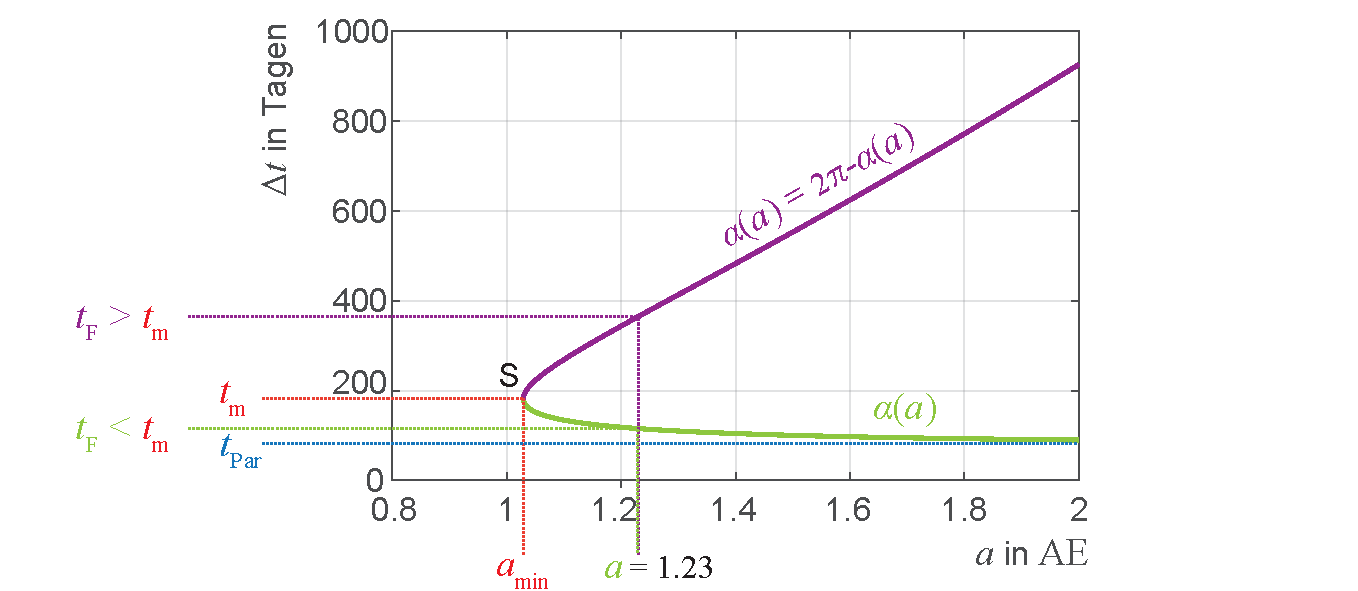
\includegraphics[width=\textwidth]{LambertProblem02Zeiten.pdf} 
	\caption[L�sung des Lambert-Problems.]{L�sung des Lambert-Problems f�r folgende Parameter: $r_1 = \SI{1.0}{AE},\, r_2 = \SI{1.525}{AE},\, \gamma = 75\degree$, und einer ToF von $t_\text{F} = 115 \mathrm{d}$ \bzw $t_\text{F} = 365 \mathrm{d}.$ Siehe \mscr~\mladynref{LambertProblem02.m}.}
	\label{abb:adyn_lambert_lsg03}
\end{figure}
Wir brauchen jetzt noch, nachdem wir $a$ bestimmt haben, die Bahnparameter $e$ und $\upsilon_0$. Aus \eqref{eq:adyn_lsglambert02a} finden wir 
\begin{align}
    E_1 = \arccos \lk \frac{a-r_1}{a\,e} \rk  \label{eq:adyn_lsglambert13}
\end{align}
und aus \eqref{eq:adyn_lsglambert02b} auch $\upsilon_0$
\begin{align}
    \upsilon_0 = \upsilon_1 - 2\,\arctan\lk \sqrt{\frac{1+e}{1-e}}\,\tan\frac{E_1}{2}\rk\,.  \label{eq:adyn_lsglambert14}
\end{align}
Setzen wir das gefundene $a$ in die Gleichungen f�r $\alpha$ und $\beta$ ein und diese wiederum in die f�r $\varphi$ und $\psi$ finden wir mit \eqref{eq:adyn_lsglambert02b} f�r die Exzentrizit�t
\begin{align}
    e = \sqrt{\frac{\lk r_2-r_1\rk^2}{\lk2a\,\sin\psi\rk^2}+\cos^2\varphi}\,.  \label{eq:adyn_lsglambert15}
\end{align}

Hat man mittels Bisektionsverfahren entweder $p$  (mit \mscr~\mladynref{LambertProblem01.m}) oder $a$  (mit \mscr~\mladynref{LambertProblem02.m}) bestimmt, kann man �ber folgende  Beziehung die Geschwindigkeiten an den Punkten $\mathrm{P}_1$ nach $\mathrm{P}_2$ auf der Trajektorie bestimmen (\cite{Walter2018, Battin1999}:
\begin{align}
\begin{split}
    \vec{v}_\text{tr, 1} &= \sqrt{\frac{\mu\,p}{r_1\,r_2\,\sin\gamma}}\,\lek \lk \vec{r}_2 - \vec{r}_1 \rk  + \frac{r_2}{p}\,\lk 1- \cos\gamma \rk\,\vec{r}_1 \rek \\
    \vec{v}_\text{tr, 2} &= \sqrt{\frac{\mu\,p}{r_1\,r_2\,\sin\gamma}}\,\lek \lk \vec{r}_2 - \vec{r}_1 \rk  + \frac{r_1}{p}\,\lk 1- \cos\gamma \rk\,\vec{r}_2 \rek \,.
\end{split}  \label{eq:adyn_lambert16}
\end{align}
Die Richtung der Periapsis (Perihel, Perig�um \usw) und damit der Wert f�r $\upsilon_0$ kann dann �ber den Laplace-Vektor\index{Laplace-Vektor} $\vec{e}$ und \eqref{eq:hm_laplace_int} aus \kap{hm_abl_kepler} wie folgt bestimmt werden:
\begin{align}
    \vec{e} &= \lk \frac{1}{r_1} - \frac{1}{a} \rk \, \vec{r}_1  - \frac{1}{\mu} \, \lk \vec{r}_1 \cdot \vec{v}_\text{tr, 1} \rk \, \vec{v}_\text{tr, 1} \,. 
		\label{eq:adyn_lambert17}
\end{align}

Wir haben das Bisektionsverfahren zur L�sung des Lambert-Problems exemplarisch f�r zwei verschiedene F�lle im \mscr~\mladynref{LambertProblem01.m} \bzw \mscr~\mladynref{LambertProblem02.m} hinterlegt. Fall 1 ist der Transfer einer Raumsonde von der ISS aus $h \approx \SI{422}{\km}$ in die Stratosph�re ($h \approx \SI{22}{\km}$) innerhalb von 50 min und Fall 2 ein Raumflug von der Erde zum Mars f�r eine Flugdauer von 115 Tagen. \figref{adyn_lambert_lsg04} und Tabelle \ref{tab:adyn_bisection} zeigen den Verlauf der Iteration f�r den Fall 2.\\

Im \mscr~\mladynref{LambertProblem03.m} haben wir die Rechnungen mit einer modernen, stabileren numerischen Routine zur L�sung des Lambert-Problems (\cite{Mahooti2015}) wiederholt. Die Routine basiert auf den Ans�tzen, die in \cite{Battin1999, Izzo2015, Walter2018} ausf�hrlich beschrieben sind. Sie beinhaltet auch hyperbolische L�sungen. Die �bereinstimmung mit dem Bisektionsverfahren f�r die angegebenen Beispiele ist sehr gut.

\begin{figure}[H]
	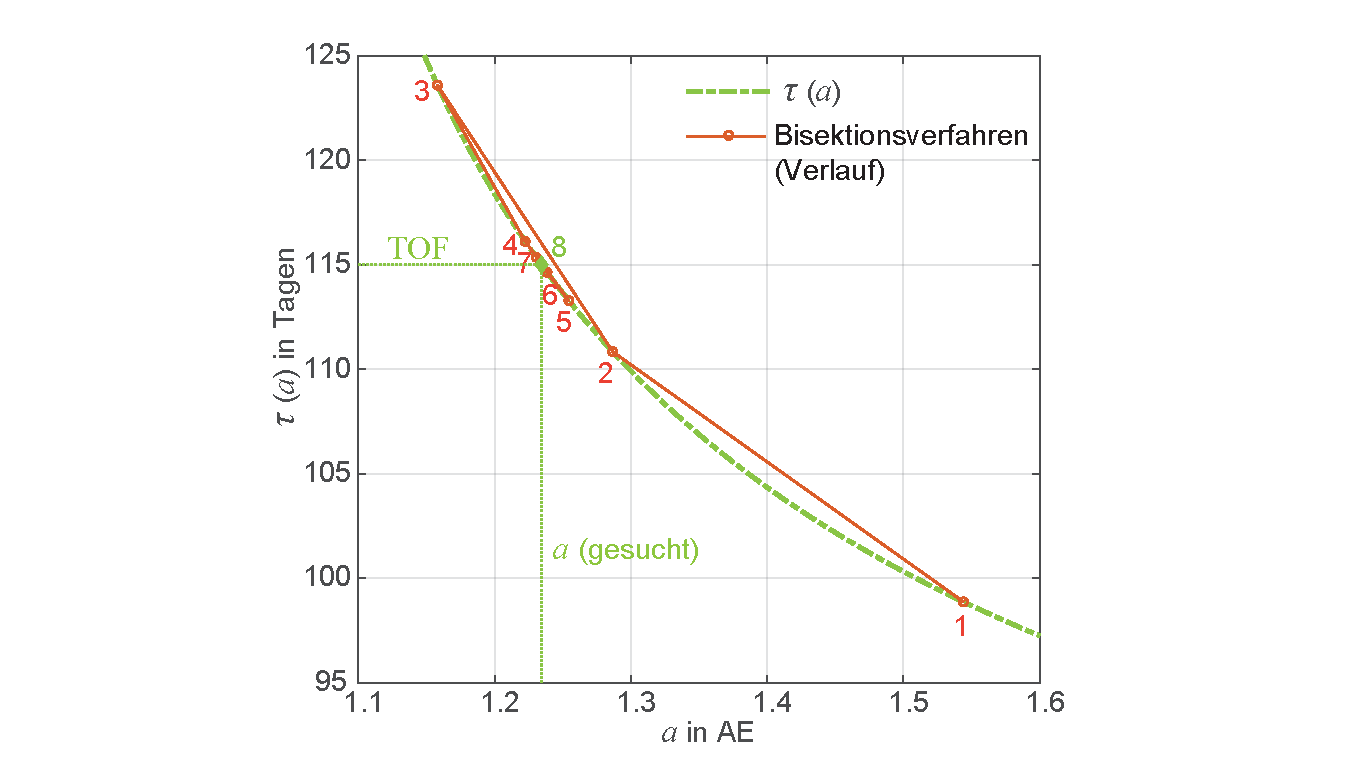
\includegraphics[width=\textwidth]{BisektionLambert.pdf} 
	\caption[Bisektionsverfahren zur L�sung des Lambert-Problems.]{Bisektionsverfahren zur L�sung des Lambert-Problems f�r folgende Parameter: $r_1 = \SI{1.000}{AE},\, r_2 = \SI{1.525}{AE},\, \gamma = 75\degree$, und einer ToF von $t_\text{F} = 115\,\mathrm{d}$. Siehe \mscr~\mladynref{LambertProblem02.m}.}
	\label{abb:adyn_lambert_lsg04}
\end{figure}

\begin{table}[ht]
\begin{center}
\begin{tabular}{L{1cm}R{1.5cm}R{1.5cm}R{1.5cm}R{2cm}R{2cm}R{1.5cm}}
    \hline
    \rule{0pt}{3pt}&&&&&& \\
      $n$ & $a_n$ & $\alpha_n$ & $\beta_n$ & $\tau(\alpha_n)$ & $\tau(\alpha_n) - \mathrm{ToF} $ & $e_n$\\
    %\rule{0pt}{3pt}&&&&&& \\
       & $\SI{}{AE}$ &&& Tage & Tage & \\
    \rule{0pt}{3pt}&&&&&& \\
    \hline
    \rule{0pt}{3pt}&&&&&& \\
 \rule{0pt}{3pt} 1    &   1.544     &   1.911    &   0.798     &   98.87      &   -16.132      &   0.387 \\
 \rule{0pt}{3pt} 2    &   1.287     &   2.214    &   0.879     &  110.83      &    -4.166      &   0.330 \\
 \rule{0pt}{3pt} 3    &   1.158     &   2.462    &   0.931     &  123.60      &     8.596      &   0.350 \\
 \rule{0pt}{3pt} 4    &   1.222     &   2.324    &   0.904     &  116.12      &     1.120      &   0.332 \\
 \rule{0pt}{3pt} 5    &   1.255     &   2.267    &   0.891     &  113.28      &    -1.723      &   0.330 \\
 \rule{0pt}{3pt} 6    &   1.238     &   2.295    &   0.898     &  114.64      &    -0.358      &   0.331 \\
 \rule{0pt}{3pt} 7    &   1.230     &   2.309    &   0.901     &  115.37      &     0.366      &   0.331 \\
 \rule{0pt}{3pt} 8    &   1.234     &   2.302    &   0.899     &  115.00      &     0.000      &   0.331 \\
    \rule{0pt}{3pt}&&&&&& \\
    \hline
\end{tabular}    
\end{center}
\caption{Bisektionsverfahren zur L�sung des Lambert-Problems. Parameter siehe Text \bzw \figref{adyn_lambert_lsg04}.}
 %f�r folgende Parameter: $r_1 = \SI{1.0}{AE},\, r_2 = \SI{1.525}{AE},\, \gamma = 75\degree$, und einer ToF von $t_\text{F} = 115 \mathrm{d}$ \bzw $t_\text{F} = 365 \mathrm{d}.$ Siehe \mscr\mladynref{LambertProblem02.m}.}
\label{tab:adyn_bisection}
\end{table}


\end{sol} 

\textcolor{blue} {$\rightarrow$ zur} \probref{adyn_manoevers4}.\\
\noindent\rule[1ex]{\textwidth}{0.5pt}  \newpage  \clearpage

%-----------------------------------------------------------------------------------------------------------

\begin{sol}{prob:adyn_manoevers5}\label{lsg:adyn_manoevers5} %�bung16
\textbf{Venus- und Mars-Fl�ge}\\

Wir bestimmen als erstes die Flugzeit f�r eine Parabell�sung von der Erdbahn (Punkt $\text{P}_1$) zur Marsbahn (Punkt $\text{P}_2$). Diese l�sst sich aus der Barker-Gleichung\index{Barker-Gleichung} \eqref{eq:hm_Barker_glg} bestimmen (siehe L�sung zu \probref{adyn_manoevers4} und\cite{Izzo2015}, \cite{sangra2021}):
			\begin{align}
								t_\text{Par} &= \frac{\sqrt{2}}{3}\,\sqrt{\frac{s^3}{\mu}}\,\lk 1-\sqrt{\lk\frac{s-c}{s}\rk^3}\rk\,.\label{eq:adyn_lsglambert21}
			\end{align}
Wir verweisen auf das \mscr~\mladynref{FlugVenusParabelbahn.m}, in welchem die Parabel-Flugbahn einer Raumsonde zur Venus
zu verschiedenen Startzeiten auf Basis der der L�sung des Lambert-Problems numerisch berechnet wird. Vorgegeben ist das Startdatum, gesucht ist das Ankunftsdatum mit dem
schnellsten Transfer unab�ngig vom notwendigen Antriebsbedarf.

\begin{figure}[H]
	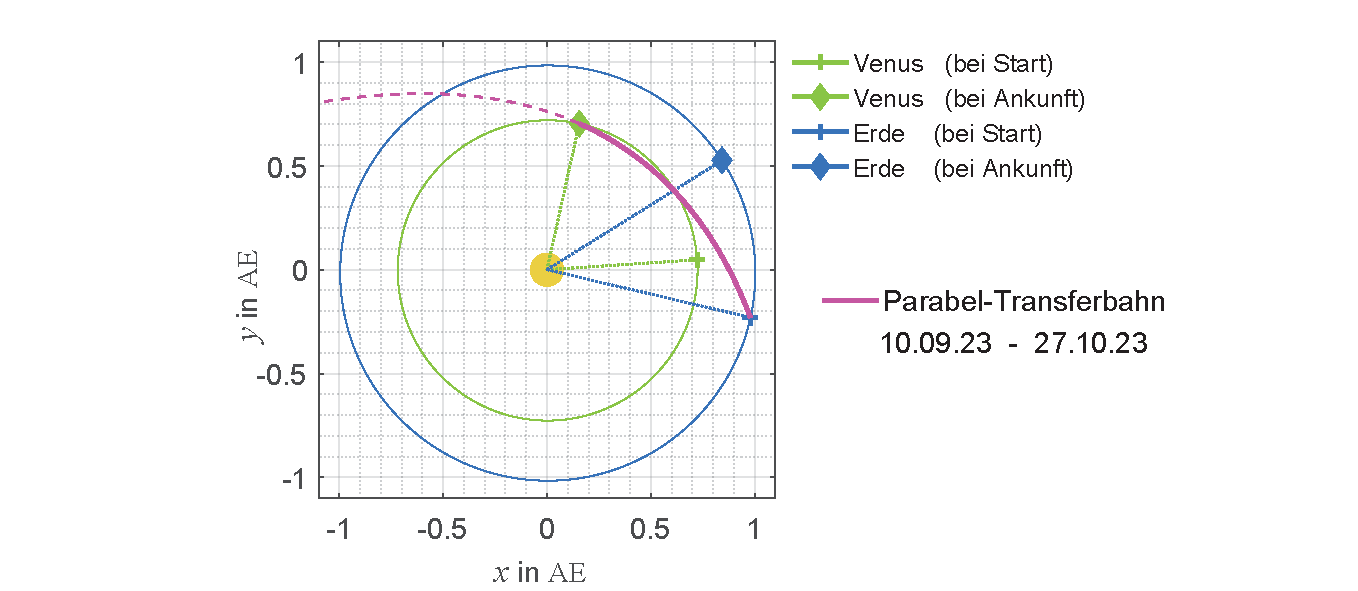
\includegraphics[width=\textwidth]{ParabelTransferVenus.pdf} 
	\caption[Parabel-L�sung des Lambert-Problems.]{Parabel-L�sung des Lambert-Problems f�r einen Flug zur Venus. Siehe \mscr~\mladynref{FlugVenusParabelbahn.m}.}
	\label{abb:adyn_lambert_lsg05}
\end{figure}

F�r die Berechnung der Transferbahn (elliptisch) von der Erde zur Venus oder zum Mars bei vorgegebener ToF benutzen wir die \mscr~\mladynref{LambertProblem03.m} \bzw \mladynref{LambertMarsVenus.m}, in welchen �ber die Routine \mladyniref{LambertSolver3.m}. die Parameter des interplanetaren Raumflugs zum Mars bzw. zur Venus �ber die L�sung des Lambert-Problems berechnet werden. Vorgegeben sind dabei die Positionsvektoren 1 und 2, sowie die Abflug und Ankunftszeit. Die Abflugs-Ankunfs-Positionen m�ssen vorher berechnet werden (z.B. �ber \mscr~\mladynref{FlugzeitenMarsVenus.m} oder �ber Programme aus dem Kapitel Himmelsmechanik, wie \mscr~\mlhmref{PlanetenbahnenKepler.m} und \mlhmref{PlanetenPositionen.m}. \\

\begin{figure}[H]
	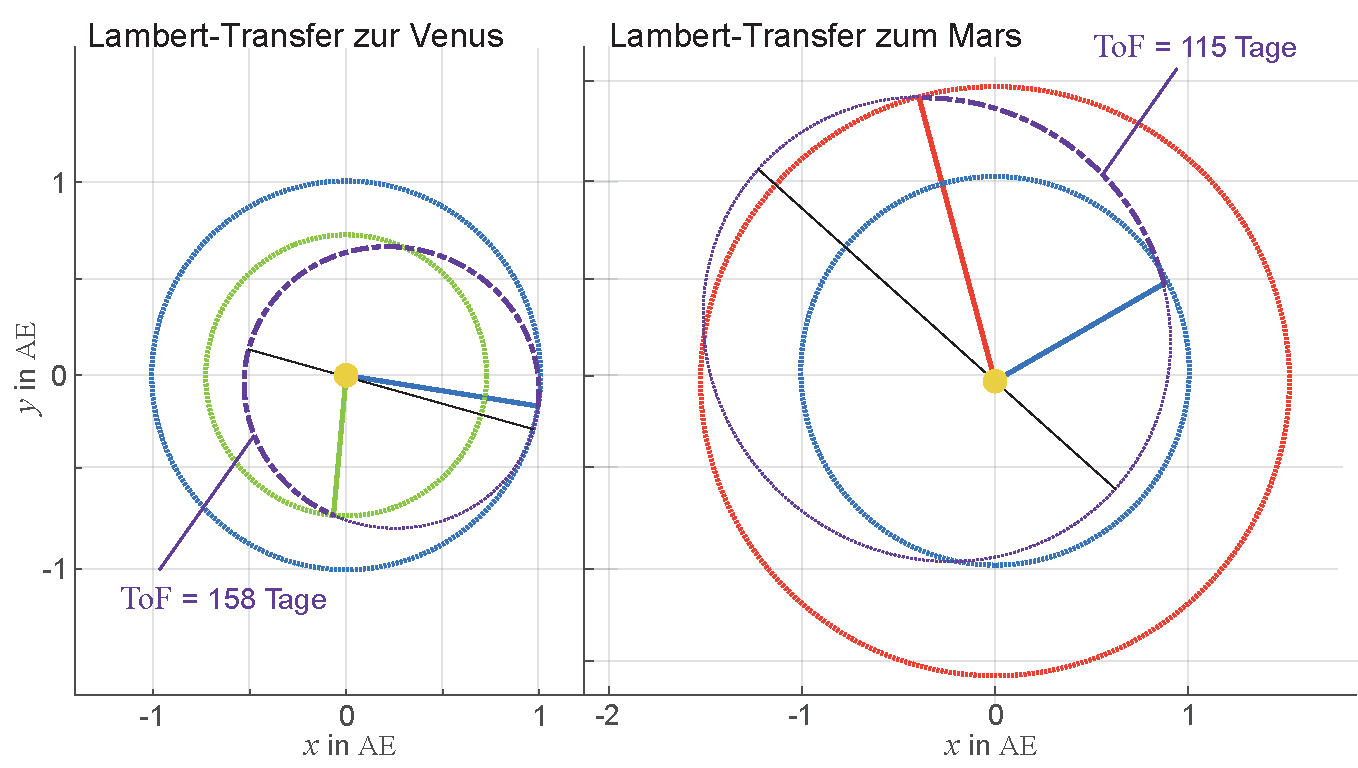
\includegraphics[width=\textwidth]{LambertTransferVenusMars.pdf} 
	\caption[L�sung des Lambert-Problems f�r Fl�ge zu Venus und Mars.]{L�sung des Lambert-Problems f�r Fl�ge zu Venus und Mars. Siehe \mscr~\mladynref{LambertProblem03.m}.}
	\label{abb:adyn_lambert_lsg06}
\end{figure}

\end{sol} 
\textcolor{blue} {$\rightarrow$ zur} \probref{adyn_manoevers5}.\\
\noindent\rule[1ex]{\textwidth}{0.5pt}  \newpage  \clearpage

%-----------------------------------------------------------------------------------------------------------

\begin{sol}{prob:adyn_manoevers6}\label{lsg:adyn_manoevers6} %�bung17
\textbf{Abfang ballistischer Raketen}\\

Die L�sung ist  im \mscr~\mladynref{LambertICBM.m} detailliert und mit ausf�hrlichen Kommentaren hinterlegt.
Die Vorgehensweise ist dabei wie folgt:
\begin{enumerate}[1.]
	\item Aus den gegebenen Werten f�r $\vec{R}$ und $\vec{V}$ der ICBM bestimmt man die Bahnparameter der ICBM. Wir verweisen auf \probref{adyn_orbits1}.
	\item Man berechnet mit diesen Bahnparametern �ber die Kepler-Gleichung \bzw die Methode mit den Gau�-Vektoren (PQR) (siehe \kap{hm_bahnen_hk_PQR}) den zeitlichen Verlauf der Trajektorie der ICBM und insbesondere den Punkt $\vec{R}(t_1+\mathrm{ToF})$, den diese nach $\mathrm{ToF}=\SI{30 }{\minute}$ errreicht. Wir erhalten:
\begin{align}
    \vec{R}(t_1+\mathrm{ToF})=[3930.7, 9762.2, 1583.3]\,\SI{}{\km}\,.
\end{align}
	\item F�r den Abf�nger gilt das Lambert-Problem mit $[\mathrm{P}_1,\mathrm{P}_2] = [\vec{r}(t_1), \vec{R}(t_1+\mathrm{ToF})]$.
	\item Man �berpr�ft, ob es �berhaupt eine L�sung geben kann. Dazu bestimmt man die minimale Flugzeit zu $t_\text{par} = \SI{16.0}{\minute}$ und die maximale Flugzeit zu $t_\text{m} = \SI{33.6}{\minute}$. Unsere $\mathrm{ToF}$ liegt dazwischen, es gibt also eine L�sung.
	\item Wir l�sen das Lambert-Problem wieder durch das in \probref{adyn_manoevers4} eingef�hrte Bisektionsverfahren und erhalten:
\begin{align}
    a=\SI{6130.7}{\km}\,,~~~\alpha = 2.9841\,,~~~\beta = 1.5418\,.
\end{align}
	\item Wir bestimmen mit diesen $a$, $\alpha$ und $\beta$ noch die notwendige Geschwindigkeit $\vec{v}_\text{trans}(t_1)$, die der Abf�nger am Punkt $\mathrm{P}_1$ haben muss, damit er auf die richtige Abfangbahn gelangt. Sie ergibt sich aus \eqref{eq:adyn_lambert08}zu:
\begin{align}
    \vec{v}_\text{trans}(t_1) &= (A+B)\,\vec{e}_c - (A-B)\,\vec{e}_1 = [2.16, 6.61, 1.13]\,\SI{}{\km\per\second}\, \\
		&\text{mit}\nonumber\\
		A &= \sqrt{\frac{G\,m_\text{E}}{4a}}\,\cot\frac{\alpha}{2}\,~~~~B = \sqrt{\frac{G\,m_\text{E}}{4a}}\,\cot\frac{\beta}{2}\,.\nonumber
\end{align}	
	\item Damit kann man sofort den erforderlichen Antriebsbedarf ermitteln, den man aufbringen muss, um den Abf�nger auf den richtigen Kurs zu bringen. Man erh�lt:
	\begin{align}
    \Delta \vec{v} &= \vec{v}_\text{trans}(t_1) - \vec{v}_1 = [4.66, 0.12,-1.37]\,\SI{}{\km\per\second}\,.		\\
		&\text{bzw}\nonumber\\
    \Delta v &= \SI{4.863}{\km\per\second}\,.
\end{align}	
	\item Zum Schlu� kann man aus $\vec{v}_\text{trans}(t_1)$ und $\vec{r}_1$ noch analog \probref{adyn_orbits1} die Bahnparameter der Abfangbahn berechnen und daraus mittels der Gau�-Vektoren-Methode (siehe \kap{hm_bahnen_hk_PQR}) die Trajektorie des Abf�ngers bestimmen, der sein Ziel nach genau 30 min erreicht (\figref{LambertAbfangICBM}).
\end{enumerate}

\begin{figure}[H]
	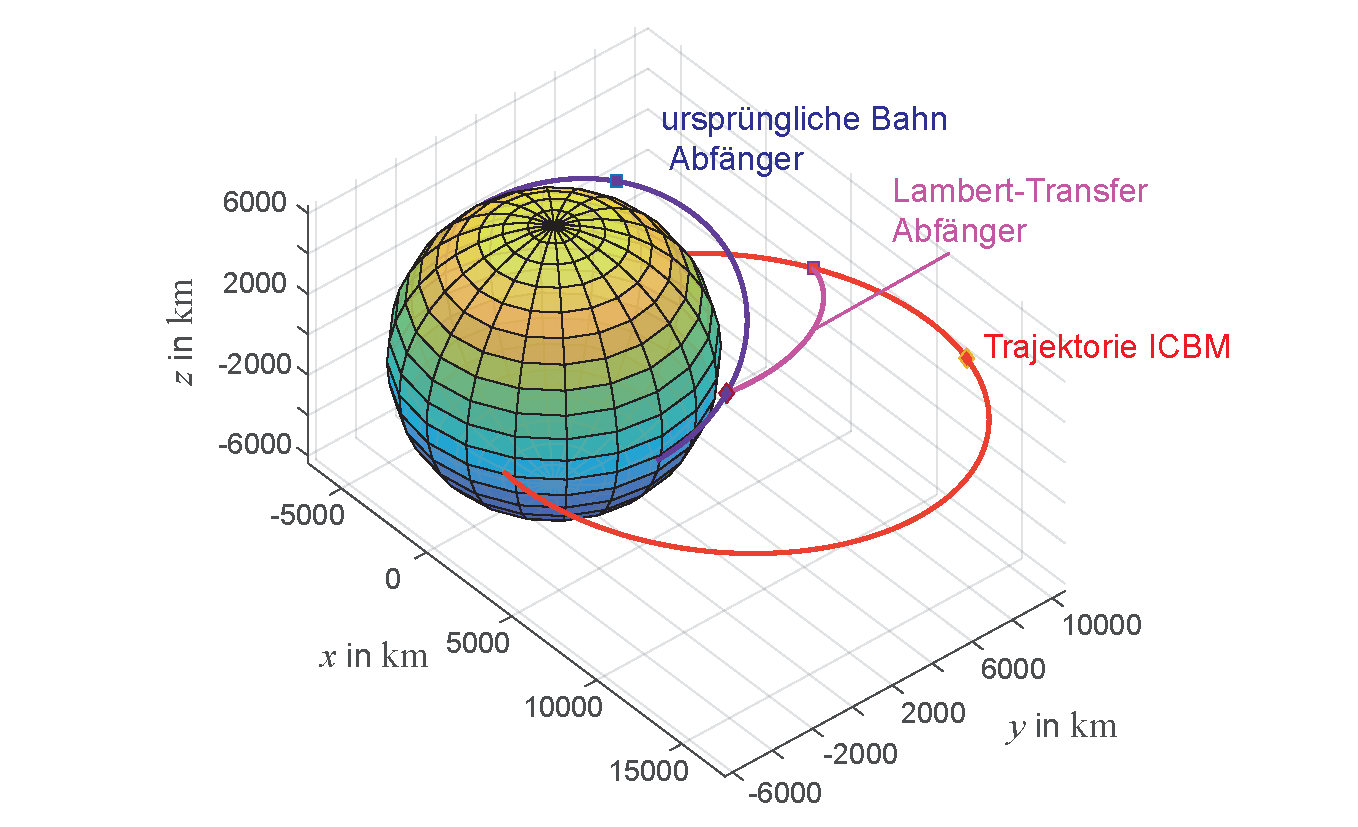
\includegraphics[width=\textwidth]{LambertAbfangICBM.pdf} 
	\caption[Abfang ballistischer Raketen.]{Abfang ballistischer Raketen. Dargestellt sind die Trajektorien der ICBM und des Abf�ngers mit und ohne $\Delta v$. Parameter siehe Text.}
	\label{abb:LambertAbfangICBM}
\end{figure}


\end{sol} 
\textcolor{blue} {$\rightarrow$ zur} \probref{adyn_manoevers6}.\\
\noindent\rule[1ex]{\textwidth}{0.5pt}  \newpage  \clearpage

%-----------------------------------------------------------------------------------------------------------

\begin{sol}{prob:adyn_manoevers7}\label{lsg:adyn_manoevers7} %�bung18
\textbf{Mondflug mit Ionenstrahltriebwerk}

\begin{itemize}
	\item
	Die Rechnungen sind im \mscr~\mladynref{Ionenantrieb02.m} ausgef�hrt und in \figref{IonenantriebExakt} dargestellt. Man sieht, dass die N�herung von \kap{adyn_kont_maneuver} zusammenbricht, wenn die Radius�nderung der Bahn per Umlauf gr��er wird.

\begin{figure}[H]
	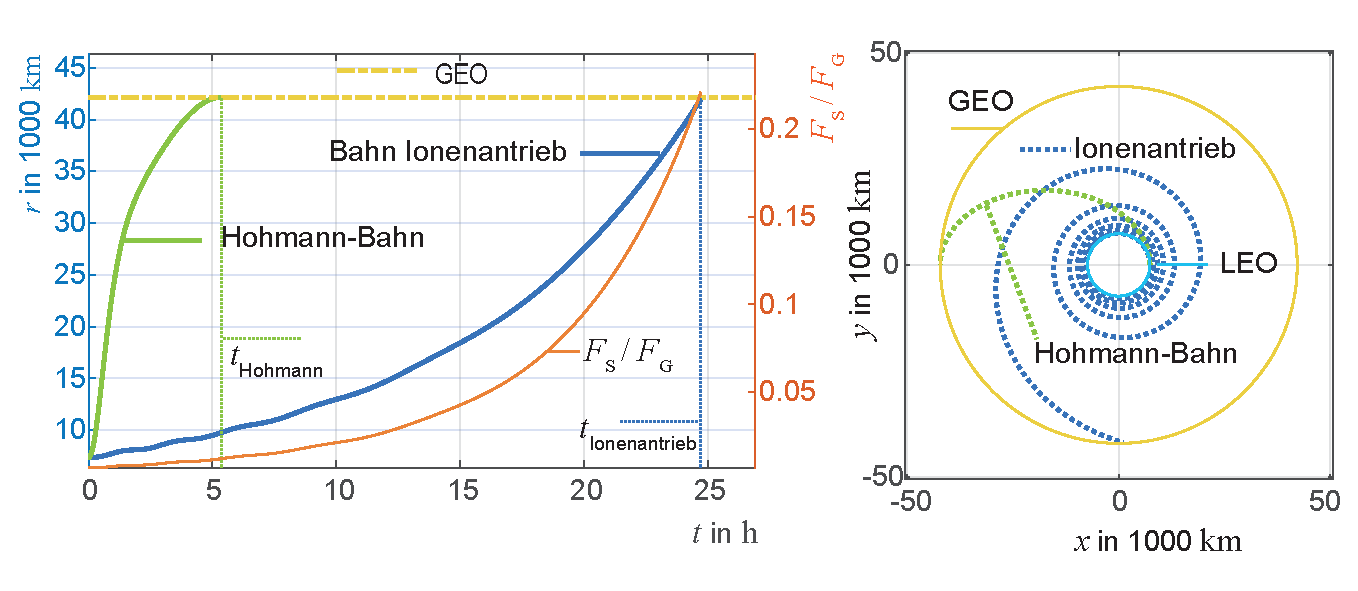
\includegraphics[width=\textwidth]{IonenantriebExakt.pdf} 
	\caption[Vergleich Hohmann-Transfer und Ionenantrieb.]{Vergleich Hohmann-Transfer und Ionenantrieb (LEO zu GEO), numerische L�sung der Bewegungsgleichung \eqref{eq:adyn_ionentr_01} f�r ein Triebwerk mit kontinuierlichem Schub. F�r den Ionenantrieb wurde ein konstanter Schub von $\SI{0.5}{\newton}$ angesetzt. Der Massenaussto� wurde bei der numerische Rechnung ber�cksichtigt.}
	\label{abb:IonenantriebExakt}
\end{figure}

	\item Die Rechnungen sind im \mscr~\mladynref{IonenantriebMond.m} ausgef�hrt. Dabei wurde die Triebwerksleistung entlang der Bahn linear so reduziert, dass sie bei der Entfernung, die dem Abstand des Lagrange-Punkts $\text{L}_1$ zwischen Erde und Mond entspricht, Null wird. Danach bewegt sich die Sonde allein im Gravitationsfeld des Mondes. Der Hohmann-Transfer wurde ebenfalls unter Ber�cksichtigung der Gravitationswirkung des Mondes berechnet.
Das Ergebnis der Rechnungen ist in der \figref{IonenantriebMoon} zu sehen.

\begin{figure}[H]
	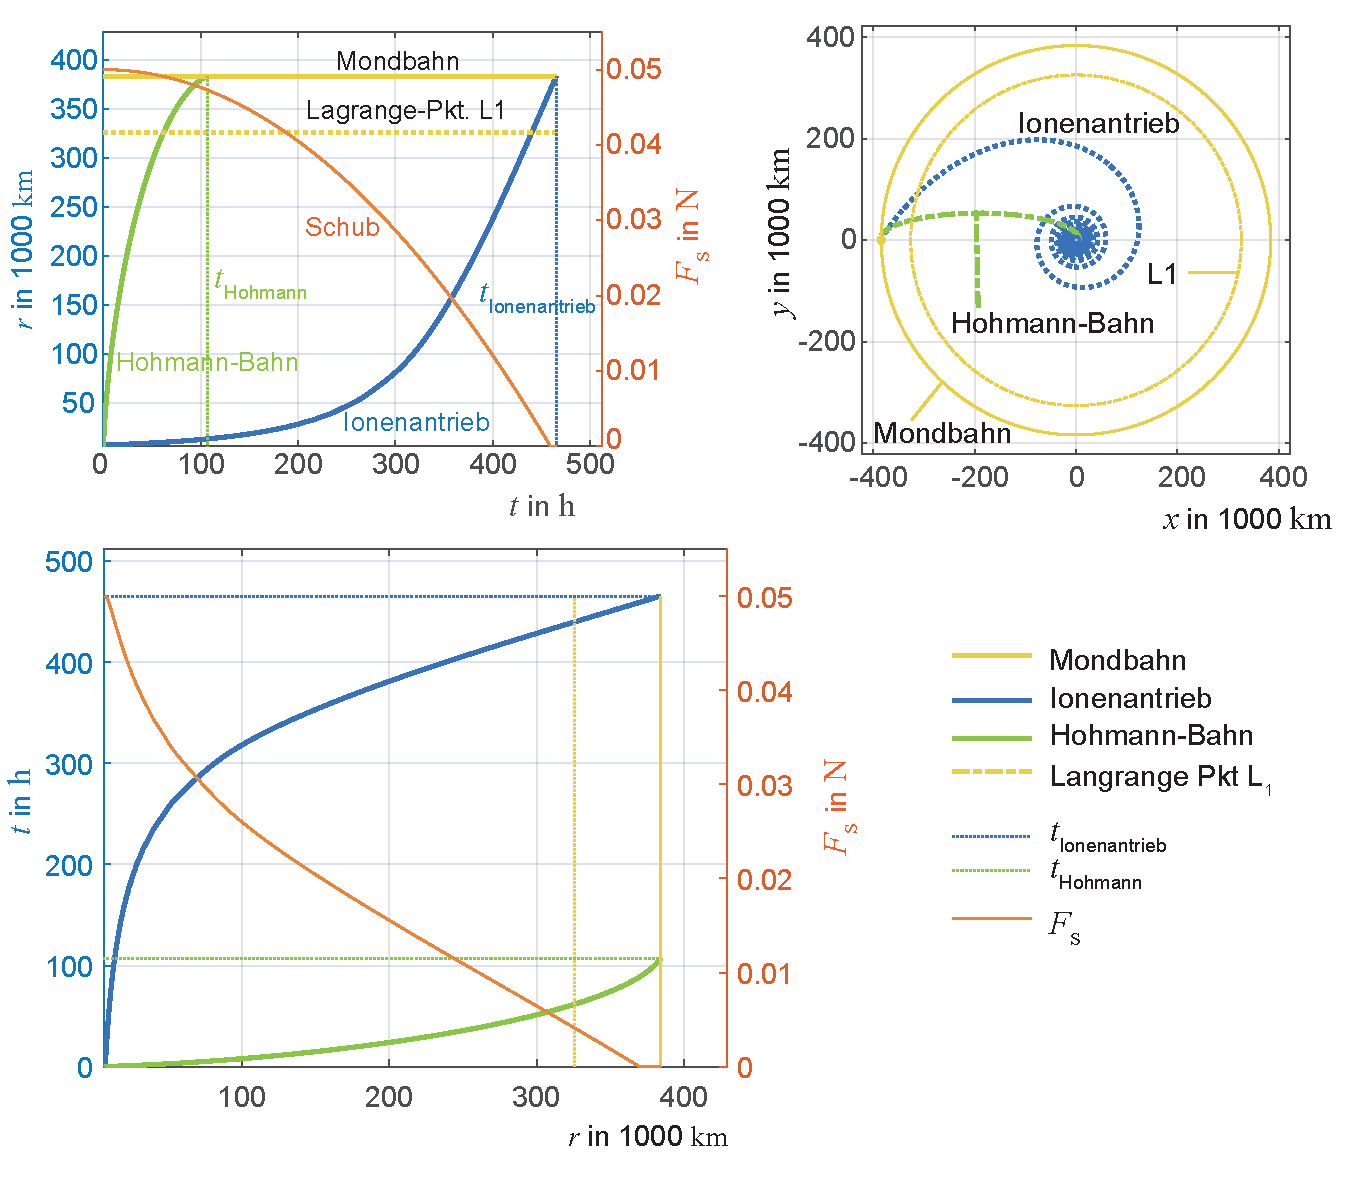
\includegraphics[width=\textwidth]{IonenantriebMoon.pdf} 
	\caption[Vergleich Hohmann-Transfer und Ionenantrieb zum Mond.]{Vergleich Hohmann-Transfer und Ionenantrieb zum Mond. F�r den Ionenantrieb wurde ein initialer Schub von $\SI{0.05}{\newton}$ der bis zum Gravitationsgleichgewicht zwischen Erde und Mond kontinuierlich reduziert wurde. Ebenso wurde der Massenaussto� bei der numerische Rechnung ber�cksichtigt.}
	\label{abb:IonenantriebMoon}
\end{figure}

\end{itemize}

\end{sol} 
\textcolor{blue} {$\rightarrow$ zur} \probref{adyn_manoevers7}.\\
\noindent\rule[1ex]{\textwidth}{0.5pt}  \newpage  \clearpage

%-----------------------------------------------------------------------------------------------------------

\begin{sol}{prob:adyn_SOI}\label{lsg:adyn_SOI} %�bung19
\textbf{Einflusssph�re - Sphere of Influence (SOI)}\\

Die Begriffe Hill-Sph�re\index{Hill-Sph�re} und Einflusssph�re\index{Einflusssph�re}\index{Sphere of Influence, SOI} adressieren zwei unterschiedliche Probleme:\\

\textit{Hill Sph�re:} Gegeben sind eine gro�e Masse $m_1$ (\zb die Sonne) und eine etwas kleinere Masse $m_2 < m_1$ (\zb die Erde) gegeben. Letztere bewegt sich um die gr��ere Masse. Es wird der Bereich gesucht, in dem f�r eine noch kleinere Masse $m_\text{M}$ (\zb der Mond) eine stabile Bahn um die kleine Masse ($m_2$) m�glich ist. Dieser Bereich wird Hill-Sph�re genannt. Die Berechnung der Hill-Sph�re hatten wir in \probref{hm_hill_sphere} ausf�hrlich behandelt und hatten dor mit $a$ als den Abstand zwischen den Massen $m_1$ und $m_2$ erhalten \eqref{eq:hm_moon_moon_lsg9}:
\begin{equation}
	r_\text{H} = a\,\sqrt[3]{\frac{1}{3}\frac{m_1}{m_2}} \,. \label{eq:adyn_hill_sphere_radius}:
\end{equation}

\textit{SOI:} Hier sind nun zwei relativ gro�e Massen $m_1, m_2$ gegeben (\zb Mars $m_1$ und Jupiter $m_2$ oder Sonne $m_2$ und Mars $m_1$ ) und eine sehr kleine Masse $m_\text{R}$ (\zb eine Raumsonde), die sich zwischen diesen beiden Massen bewegt. Es werden die Bereiche gesucht, in welchem jeweils eines der Zentren der Massen $m_1, m_2$ den Ursprung des Koordinatensystems bildet, welches f�r die Beschreibung der Bewegung der sehr kleinen Masse $m_\text{R}$  verwendet wird. In diesem Bereich muss dann f�r die Berechnung der Bewegung nur die Gravitationskraft der jeweiligen die SOI definierenden Masse $m_1$ oder $m_2$ ber�cksichtigt werden. Damit kann in der Astrodynamik bei interplanetaren Raumfl�gen die Trajektorie oft durch Aneinanderf�gen von Kepler-Bahn Abschnitten in den aufeinanderfolgenden SOI der einzelnen Planeten \bzw der Sonne (im interplanetaren Raum) n�herungsweise berechnet werden (sogenannte \textit{patched conic trajectories}.\\
Zur Herleitung der Beziehung f�r den Radius der SOI als Funktion der Massen  $m_1, m_2$ verwendet man zwei Referenzsysteme:
\begin{itemize}
	\item Zum einen erfolgt die Betrachtung der Bewegung der Raumsonde in einem Koordinaten\-system, dessen Ursprung im Zentrum der Masse $m_1$ liegt und ber�cksichtigt als Hauptwirkung nur die Gravitation der Masse $m_1$. Die Gravitationsbeschleunigung der gr��eren Masse $m_2$ wird in der Bewegungsgleichung als St�rgr��e eingef�hrt, im Prinzip als erste Abeitung.
	\item Dann betrachtet man die Bewegung der Raumsonde in dem \KOS, dessen Ursprung im Zentrum der Masse $m_2$ liegt und ber�cksichtigt als Hauptwirkung nur die Gravitation der Masse $m_2$. In der Bewegungsgleichung wird dann wiederum die Gravitationsbeschleunigung der Masse $m_1$ als St�rgr��e eingef�hrt.
\end{itemize}

\begin{figure}[H]
	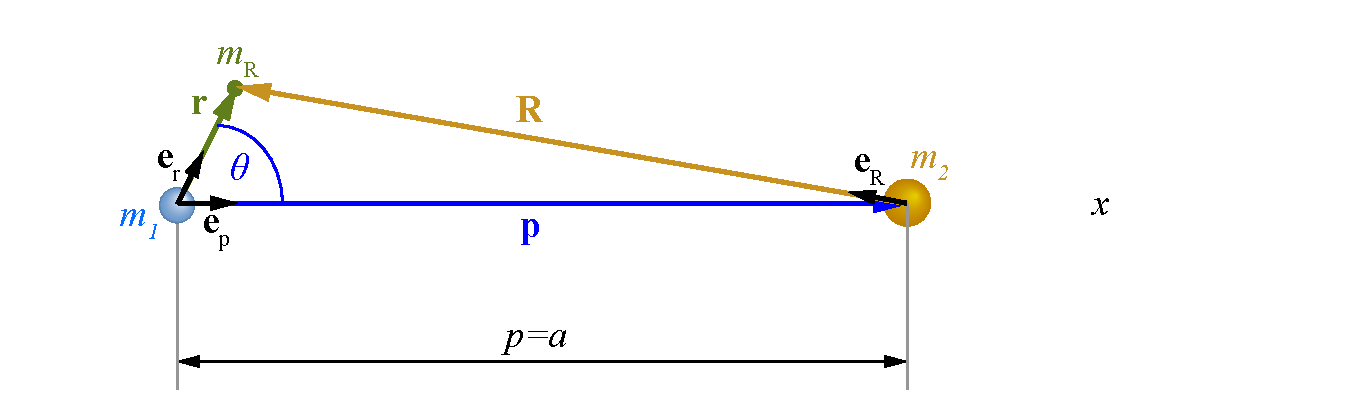
\includegraphics[width=\textwidth]{GeometrieHerleitungSOI.pdf} 
	\caption[Zur Herleitung der Einflusssph�re.]{Zur Herleitung der Einflusssph�re.}
	\label{abb:adyn_SOI01}
\end{figure}

Es ergeben sich folgende Bewegungsgleichungen (f�r $m_\text{R} \ll m_1,m_2$):\footnote{Die Herleitung wird als Zusatz�bung empfohlen, siehe auch \kap{hm_potentialtheorie} sowie \figref{adyn_SOI01}.}
\begin{subequations}
\begin{align}
    \ddot{\vec{r}} &= -G\,m_1\,\frac{\vec{r}}{r^3}-G\,m_2\,\lk\frac{\vec{p}}{p^3} + \frac{\vec{R}}{R^3}\rk\,,\\
    \ddot{\vec{R}} &= -G\,m_2\,\frac{\vec{R}}{R^3}-G\,m_1\,\lk\frac{\vec{r}}{r^3} - \frac{\vec{p}}{p^3}\rk\,.
\end{align}    \label{eq:adyn_SOI01}
\end{subequations}

Diese Gleichungen k�nnen geschrieben werden als:
\begin{subequations}
\begin{align}
     \ddot{\vec{r}} &= \vec{a}_{\text{H},1}^{\lk 1 \rk} + \vec{a}_{\text{S},2}^{\lk 1 \rk}\,, \\
     \ddot{\vec{R}} &= \vec{a}_{\text{H},2}^{\lk 2 \rk} + \vec{a}_{\text{S},1}^{\lk 2 \rk} \,,
\end{align} \label{eq:adyn_SOI02}
\end{subequations}

worin in $\vec{a}_{\text{H,S},i}^{\lk j \rk}$ der Index $j$ das KOS-System des jeweiligen Planeten bezeichnet und H und S f�r die Hauptgravitations- \bzw St�rbeschleunigung stehen. Letztere wird hervorgerufen jeweils durch die Masse $m_i$ ($i=1,2$). Die Beschleunigungen k�nnen mit den Einheitsvektoren $\vec{e}_\text{r},\, \vec{e}_\text{R}$ und $\vec{e}_\text{p}$aus \figref{adyn_SOI01} beschrieben werden durch:

\begin{subequations}
\begin{align}
   \vec{a}_{\text{H},1}^{\lk 1 \rk} &= -\frac{G\,m_1}{r^2}\,\vec{e}_\text{r}\,,\label{eq:adyn_SOI03a} \\ 
    \vec{a}_{\text{H},2}^{\lk 2 \rk} &= -\frac{G\,m_2}{R^2}\,\vec{e}_\text{R}\,, \label{eq:adyn_SOI03b} \\
    \vec{a}_{\text{S},2}^{\lk 1 \rk} &= +\,G\,\frac{m_2}{p^2}\,\sum\limits_{k=1}^\infty \lk \frac{r}{p}\rk^k\lek {\PL {k+1}}'\lk  \cos\theta\rk\,\vec{e}_\text{p} - {\PL {k}}'\lk\cos\theta\rk\,\vec{e}_\text{r} \rek\,, \label{eq:adyn_SOI03c} \\ 
    \vec{a}_{\text{S},1}^{\lk 2 \rk}&= +\,G\,\frac{m_1}{r^2}\,\lek \lk \frac{r}{p} \rk^2\,\vec{e}_\text{p} - \vec{e}_\text{r} \rek\,, \label{eq:adyn_SOI03d}
\end{align} \label{eq:adyn_SOI03}
\end{subequations}  

worin $\PL k$ die im \kap{hm_potentialtheorie} eingef�hrten Legendre-Polynome sind (\cite{Andrews2003}) und ${\PL k}'$ deren erste Ableitungen. 
Die Gleichungen sind direkt aus \eqref{eq:adyn_SOI01} ablesbar. Lediglich Gleichung \eqref{eq:adyn_SOI03b} erfordert eine Nebenrechnung. Sie ergibt sich aus der Definition der Legendre-Polynome und der Nutzung der verschiedenen Beziehungen zwischen den Ableitungen und den Rekursionsformeln (\cite{Riley2006, Andrews2003}). 
Wir bilden nun die Verh�ltnisse von Hauptbeschleunigung zu St�rbeschleunigung im jeweiligen \KOS. Wir dividieren dazu \eqref{eq:adyn_SOI03d} durch \eqref{eq:adyn_SOI03b} und finden:
\begin{align}
    \frac{ \vec{a}_\text{S1}^{\lk 2\rk}}{ \vec{a}_\text{H2}^{\lk 2\rk}} = \frac{m_1}{m_2}= \frac{1-2\,\lk\frac{r}{p}\rk\,\cos\theta + \lk\frac{r}{p}\rk^2}{\lk\frac{r}{p}\rk^2}\,\sqrt{\lek 1-2\,\lk\frac{r}{p}\rk^2\,\cos\theta + \lk\frac{r}{p}\rk^4\rek} \,.\label{eq:adyn_SOI04}
\end{align}
Analog erh�lt man durch Division von \eqref{eq:adyn_SOI03c} durch \eqref{eq:adyn_SOI03a}:
\begin{align}
    \frac{\vec{a}_{\text{S},2}^{\lk 2\rk}}{\vec{a}_{\text{H},1}^{\lk 2\rk}} = \frac{m_1}{m_2}\,\lk \frac{r}{p} \rk^3 \, \sqrt{\lek 1+3\cos^2\theta \rek} + \mathcal{O}\lk\frac{r}{p}^4\rk \,, \label{eq:adyn_SOI05}
\end{align}
wobei wir hier wegen $r \ll p$ alle Terme mit Potenzen von $\lk \frac{r}{p} \rk^n$, $n>3$ vernachl�ssigen. Die Gleichungen dr�cken das Verh�ltnis von St�rbeschleunigung zu Hauptbeschleunigung im jeweiligen Bezugssystem aus.\\
Gleichsetzen von \eqref{eq:adyn_SOI04} mit \eqref{eq:adyn_SOI05} bedeutet, dass die St�rungs- und Hauptbeschleunigungen an einem Ort im Abstand $r_\text{SOI} $ von dem jeweiligen Zentrum des \KOS im gleichen Verh�ltnis zueinander stehen. Man erh�lt dann eine diesen Abstand unter der Annahme $r/p \ll 1$: 
\begin{align}
    \frac{r_\text{SOI}}{p} &= \sqrt[5]{\frac{m_1{}^2}{m_2{}^2}}\,\underbrace{\lk 1+3\cos^2\theta\rk^{-\frac{1}{10}}}_{\leq 1.148}~~\rightarrow ~~~ \frac{r_\text{SOI}}{p} \approx \lk \frac{m_1}{m_2}\rk^{\frac{2}{5}}\,. \label{eq:adyn_SOI06}
\end{align}
Der Radius einer SOI h�ngt somit vom Abstand $p$ beider Massen und dem Verh�ltnis (hoch $2/5$) der beiden Massen ab. Tabelle \ref{tab:adyn_SOI01} zeigt die Radien der SOI der Planeten unseres Sonnensystems im Vergleich zu den Radien der Hill-Sph�re \eqref{eq:adyn_hill_sphere_radius}:
\begin{table}[ht]
		\begin{center}
    \begin{tabular}{|C{1.5cm}|C{2.75cm}|C{2.75cm}|C{2.75cm}|C{2.75cm}|}
    \hline
    \rule{0pt}{3pt}& & &&  \\
      Planet (Masse $m_1$) & Gro�e Halbachse\linebreak zur Sonne \linebreak (Masse $m_2$)\linebreak $\lk\SI{}{\km}\rk$ & Massenverh�ltnis Planet/Sonne \linebreak $m_1/m_2$& Radius der SOI \linebreak  $\lk\SI{}{\km}\rk$ \linebreak \linebreak \eqref{eq:adyn_SOI_radius} &  Radius der Hill-Sph�re  \linebreak  $\lk\SI{}{\km}\rk$ \linebreak \linebreak \eqref{eq:adyn_hill_sphere_radius} \\
    \rule{0pt}{3pt}&& &&  \\
    \hline
    \rule{0pt}{3pt}&& &&   \\
    \rule{0pt}{6pt} Merkur &\SI{57.9e6}{}&$\SI{0.166e-6}{}$ & $\SI{112000e06}{}$& $\SI{2.206e05}{}$\\
    \rule{0pt}{3pt}&& &&   \\
    \rule{0pt}{6pt} Venus &\SI{108.2e6}{}&$\SI{2.450e-6}{}$ & $\SI{616350e06}{}$& $\SI{1.010e+06}{}$\\
    \rule{0pt}{3pt}&& &&   \\
    \rule{0pt}{6pt} Erde & \SI{149.6e6}{}&$\SI{3.002e-6}{}$ & $\SI{924510e06}{}$& $\SI{1.496e+06}{}$\\
    \rule{0pt}{3pt}&& &&   \\
    \rule{0pt}{6pt} Mars &\SI{227.9e6}{}&$\SI{0.323e-6}{}$ & $\SI{577230e06}{}$& $\SI{1.084e+06}{}$\\
    \rule{0pt}{3pt}&& &&   \\
    \rule{0pt}{6pt} Jupiter &\SI{778.6e6}{}&$\SI{954.490e-6}{}$ & $\SI{48219000e06}{}$& $\SI{5.315e+07}{}$\\
    \rule{0pt}{3pt}&& &&   \\
    \rule{0pt}{6pt} Saturn &\SI{1433.5e6}{}&$\SI{285.641e-6}{}$ & $\SI{54793000e06}{}$& $\SI{6.546e+07}{}$\\
    \rule{0pt}{3pt}&& &&   \\
    \rule{0pt}{6pt} Uranus &\SI{2872.5e6}{}&$\SI{43.651e-6}{}$ & $\SI{51791000e06}{}$& $\SI{7.013e+07}{}$\\
    \rule{0pt}{3pt}&& &&   \\
    \rule{0pt}{6pt} Neptun &\SI{4495.1e6}{}&$\SI{51.295e-6}{}$ & $\SI{86451000e06}{}$& $\SI{1.158e+08}{}$\\
    \rule{0pt}{3pt}&& &&   \\
    \hline
    \end{tabular} 
		\end{center}
		\caption{Vergleich Radien der SOI mit dem Hill-Sph�re f�r die Planeten unseres Sonnensystems.}
		\label{tab:adyn_SOI01}
\end{table}

Im letzten Schritt in \eqref{eq:adyn_SOI06} haben wir die $\theta$-Abh�ngigkeit vernachl�ssigt. Ber�cksichtigt man diese, so ergibt sich ein oblater Sph�roid anstelle einer Einflusssph�re (Sphere of Influence). In den meisten F�llen reicht die Kugelbetrachtung aber aus, man kann also schreiben:
\begin{align}
	r_\text{SOI} = a\,\sqrt[5]{\lk \frac{m_1}{m_2}\rk^2} \,, \label{eq:adyn_SOI_radius}
\end{align}
worin a der Abstand zwischen den beiden Massen (\ia gleich der gro�en Halbachse von $m_1$ um $m_2$) ist.\\
Man wird also immer dann, wenn sich die Raumsonde in geringerem Abstand als $r_\text{SOI}$  von der Masse $m_1$ befindet, die Bewegung als Zweik�rperproblem mit den Massen $m_1,\,m_\text{R}$ behandeln k�nnen, bei Abst�nden gr��er als $r_\text{SOI}$ als Zweik�rperproblem mit den Massen $m_2,\,m_\text{R}$.\\

\end{sol} 
\textcolor{blue} {$\rightarrow$ zur} \probref{adyn_SOI}.\\
\noindent\rule[1ex]{\textwidth}{0.5pt}  \newpage  \clearpage

%-----------------------------------------------------------------------------------------------------------

\begin{sol}{prob:adyn_swingby01}\label{lsg:adyn_swingby01} %�bung20
\textbf{Gravity-Assist-Man�ver - Analytische L�sung}\\

Wir beginnen mit:
\begin{subequations}
\begin{align}
        \vec{v}_1{}' &= \vec{v}_1 - \vec{v}_\text{P} \,, \label{eq:adyn_lsgswingby01a} \\
        v_1{}'^2     &= v_1{}^2 + v_\text{P}{}^2 - 2\,v_1{}'\,v_\text{P}\,\cos\gamma_1{}'\,, \label{eq:adyn_lsgswingby01b} \\
        \vec{v}_2{}  &= \vec{v}_2{}' + \vec{v}_\text{P} \,, \label{eq:adyn_lsgswingby02a} \\
        v_2{}^2      &= v_2{}'^2 + v_\text{P}{}^2 + 2\,v_2{}'\,v_\text{P}\,\cos\beta_2{}' \,, \label{eq:adyn_lsgswingby02b} \\
        v_1{}'       &= v_2{}'= v_\infty \,. \label{eq:adyn_lsgswingby02c} 
\end{align} %\label{eq:adyn_lsgswingby02} 
\end{subequations}
F�r die weitere numerische Auswertung lassen sich aus \eqref{eq:adyn_swingby01}, \eqref{eq:adyn_swingby03} und \figref{adyn_swingby01} durch Anwendung des Kosinussatzes \bzw geometrische �berlegungen aus der Streuhyperbel noch einige n�tzliche Beziehungen, \zb zwischen dem Winkel $\beta_2{}'$ und dem Streuwinkel $\vartheta'$ sowie f�r den Winkel $\varphi'$ gewinnen:
\begin{subequations}
\begin{align}
        \beta_2{}' &= \beta_1{}' -\vartheta' = \beta_1{}' + 2\varphi' - 180\degree \label{eq:adyn_lsgswingby03a} \\
        \cos\beta_2{}' &= \cos\,\beta_1{}'\,\lk 1-2\cos^2\varphi'\rk + 2\cos\varphi'\,\sqrt{1-\cos^2\varphi'}\,\sqrt{1-\beta_1'{}^2} \label{eq:adyn_lsgswingby03b} \\
        \cos\beta_1{}' &= \frac{{v_1{}}^2+v_\text{P}{}^2-{v_1{}'}^2}{2\,v_1\,v_\text{P}} \label{eq:adyn_lsgswingby03c}
\end{align}%\label{eq:adyn_lsgswingby03} 
\end{subequations}
Die Gr��e $\cos\varphi'$ k�nnen wir ebenfalls aus \figref{adyn_swingby01} mit der Hyperbelgleichung durch
\begin{align}
    \cos\varphi' &= \frac{1}{1+ (r_\text{per}\,v_1{}'^2)/(G\,m_\text{P})} = -\frac{1}{e}\,\label{eq:adyn_lsgswingby04} 
\end{align}
ausdr�cken.

\begin{nebenrechnungNeu} {} \\
Der Winkel $\varphi'$ h�ngt mit dem asymptotischen Grenzwinkel $\theta_\infty{}'$ der Hyperbel wie folgt zusammen:
\begin{align}
    \theta_\infty{}' = -\frac{1}{e} = + \cos\lk 180\degree-\varphi'\rk = - \cos\varphi' \label{eq:adyn_lsgswingby05} 
\end{align}
Die Exzentrizit�t ist nach \eqref{eq:hm_relations2} gegeben durch
\begin{align}
    e= \sqrt{1+\frac{2\,H\,L^2}{\mu_\text{P}{}^2}} = \sqrt{1+\frac{2L^2}{\mu_\text{P}{}^2}\,\frac{v_1{}'^2}{2}} = \sqrt{1 + \frac{b^2\,v_1{}'^4}{\mu_\text{P}^2}}\,, \label{eq:adyn_lsgswingby06} 
\end{align}
wobei wir $H = v_1{}'^2/2$ f�r $r\to \infty$ und $L_\infty = b\,v_1{}' = b\,v_2{}' = b\, v_\infty$ f�r $r\to \infty$ benutzt haben.\\
Wegen der Drehimpulserhaltung k�nnen wir $L_\infty$ durch $L_\text{per} = r_\text{per}\,v_\text{per}{}'$ am Perizentrum ersetzen und benutzen dabei den \textit{vis-viva}-Satz \eqref{eq:hm_vis-viva}, womit wir erhalten:
\begin{align}
    L = b\,v_1{}' = r_\text{per}\,v_\text{per}{}'~~~\text{und}~~~
    \frac{v_1{}'}{2}^2 = \frac{v_\text{per}{}'^2}{2} - \frac{\mu_\text{P}}{r_\text{per}}\,.\label{eq:adyn_lsgswingby07} 
\end{align}
\end{nebenrechnungNeu}

\newpage
Mit den Beziehungen in \eqref{eq:adyn_lsgswingby07} k�nnen wir in \eqref{eq:adyn_lsgswingby06} den Streuparameter $b$ eliminieren und erhalten aus \eqref{eq:adyn_lsgswingby02b} mit \eqref{eq:adyn_lsgswingby05} �ber \eqref{eq:adyn_lsgswingby03b} schlie�lich die heliozentrische Geschwindigkeit des Raumschiffs $v_2$ beim Verlassen der Einflusssph�re des Gravity-Assist-Planeten am Punkt $\text{P}_2$:
\begin{subequations}
    \begin{align}
        v_2{}^2 = v_1{}^2 - \frac{2\,C_1}{C_2{}^2} + \frac{4\,v_1{}'\,v_\text{P}}{C_2}\,\sqrt{1-\frac{1}{C_2{}^2}}\,\sqrt{1-\lk\frac{C_1}{2\,v_1{}'\,v_\text{P}}\rk^2}\label{eq:adyn_lsgswingby08a}
    \end{align}
    mit 
    \begin{align}
        C_1 &= v_1{}^2 - v_\text{P}^2 - v_1{}'^2 \label{eq:adyn_lsgswingby08b}\,,\\
        C_2 &= 1+\frac{r_\text{per}}{\mu_\text{P}}\,v_1{}'{}^2 \label{eq:adyn_lsgswingby08c}\,,\\
        v_1{}'&= \sqrt{v_1{}^2 +v_\text{P}{}^2 - 2\,v_1\,v_\text{P}\,\cos\gamma_1}\,.\label{eq:adyn_lsgswingby08d}
    \end{align}%\label{eq:adyn_lsgswingby08}
\end{subequations}
Wir haben $v_2(r_\text{per},\gamma_1)$ in \figref{adyn_lsgswingby01} dargestellt.

\begin{figure}[H]
	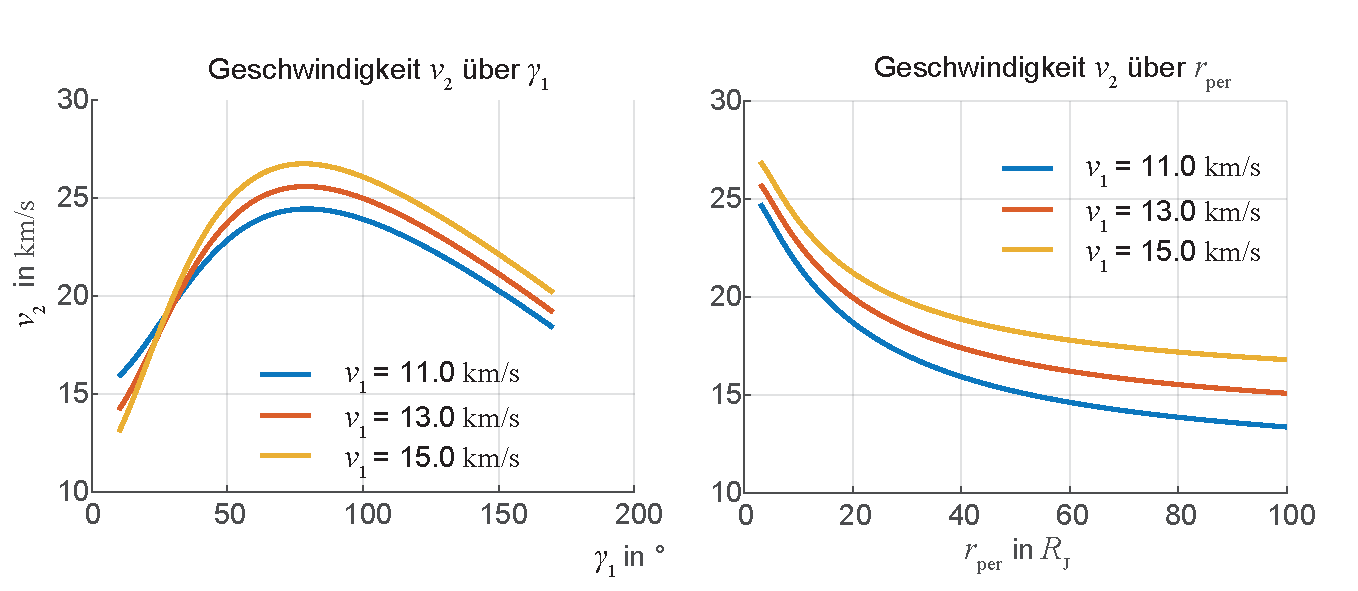
\includegraphics[width=\textwidth]{GravityAssistAnalytisch.pdf} 
	\caption[Gravity-Assist-Man�ver (Analytisch L�sung).]{Gravity-Assist-Man�ver (Analytisch L�sung).}
	\label{abb:adyn_lsgswingby01}
\end{figure}

Zum Schluss wollen wir noch den maximal m�glichen Energiegewinn bei einem Gravity-Assist-Man�ver berechnen. Dieser ergibt sich zu
\begin{align}
    \Delta H &= \frac{1}{2}\,v_2{}^2 - \frac{m_\text{S}\,G}{r_1-r_\text{per}} - \lk \frac{1}{2}\,v_1{}^2 - \frac{m_\text{S}\,G}{r_1-r_\text{per}}\rk \approx \frac{1}{2}\,\lk v_2{}^2 - v_1{}^2\rk \,.\label{eq:adyn_lsgswingby09}
\end{align}
Der Energiegewinn h�ngt also bei vorgegebenen $r_\text{per}$ von zwei Parametern ab:\\
$v_1{}'$ (\bzw. $v_1$)\, und $\beta_1{}'$ (\bzw $\gamma_1$).
Tr�gt man $\Delta H$ �ber $\beta_1{}'$ und $v_1{}'$ auf, so findet man ein Maximum bei $\beta_1{}' = 2\pi/3=120\degree$ und 
	\[v_1{}' = \sqrt{\frac{\mu_\text{P}}{r_\text{per}}}\,,
\]
Damit kann man mit den bekannten Gr��en $m_\text{P}$, $r_\text{per}$ (wir nehmen $r_\text{per} \approx 5\,R_\text{P}$ an) und $v_\text{P}$ die notwendig Anfluggeschwindigkeit $v_\text{1,opt}$ bestimmt, die den maximalen Energiegewinn bringt. Die Rechnungen sind im Detail \mscr{} \mladynref{GravityAssistAnalytik.m} ausgef�hrt. 

Der Energiegewinn $\Delta H(v_1{}', \beta_1{}')$ \bzw $\Delta H(v_1{}, \gamma_1{})$ ist in \figref{adyn_lsgswingby02a} dargestellt:

\begin{figure}[H]
	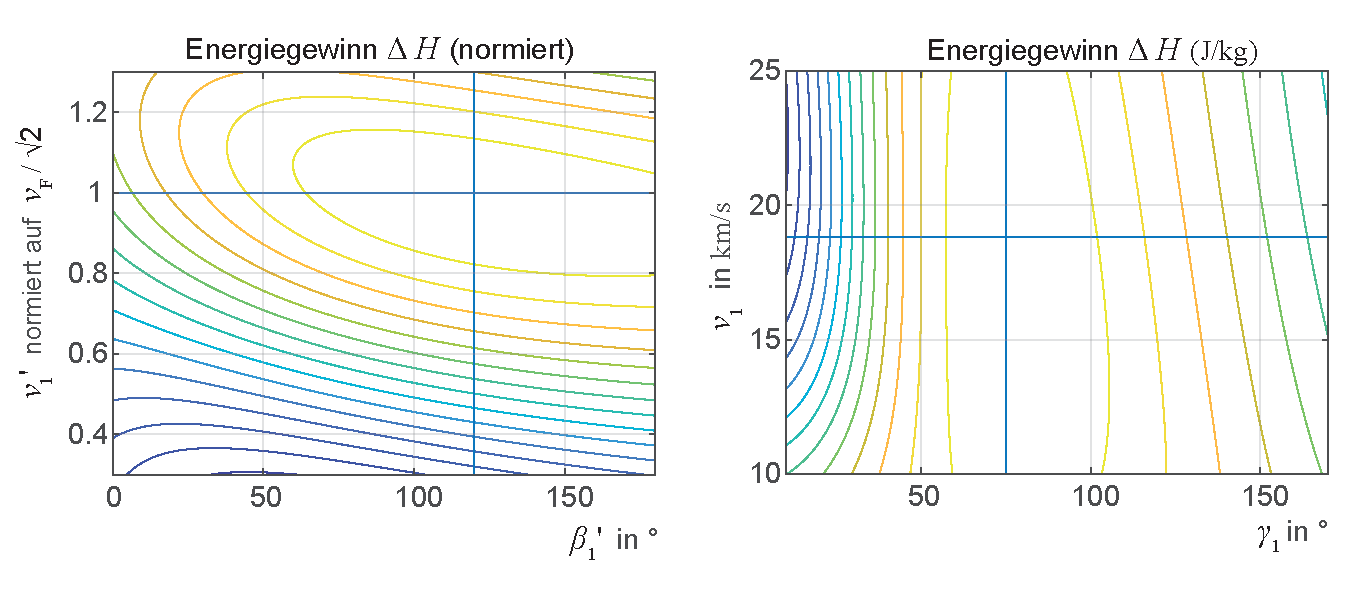
\includegraphics[width=\textwidth]{GravityAssistEnergiegewinn.pdf} 
	\caption[Gravity-Assist-Man�ver - Energiegewinn.]{Gravity-Assist-Man�ver - Energiegewinn am Beispiel des Flugs einer Raumsonde um den Jupiter.  Parameter: $r>_\text{per} = 5\,R_\text{J}$.}
	\label{abb:adyn_lsgswingby02a}
\end{figure}

\end{sol} 
\textcolor{blue} {$\rightarrow$ zur} \probref{adyn_swingby01}.\\
\noindent\rule[1ex]{\textwidth}{0.5pt}  \newpage  \clearpage
%
%%-----------------------------------------------------------------------------------------------------------

\begin{sol}{prob:adyn_swingby03}\label{lsg:adyn_swingby03} %�bung21
\textbf{Gravity-Assist-Man�ver - Simulation}\\

Die Simulation des Swing-By ist im \mscr{} \mladynref{GravityAssistSimulation.m} ausgef�hrt, die Resultate f�r ein Beispiel am Jupiter in \figref{adyn_lsgswingby02}.\\

\begin{figure}[H]
	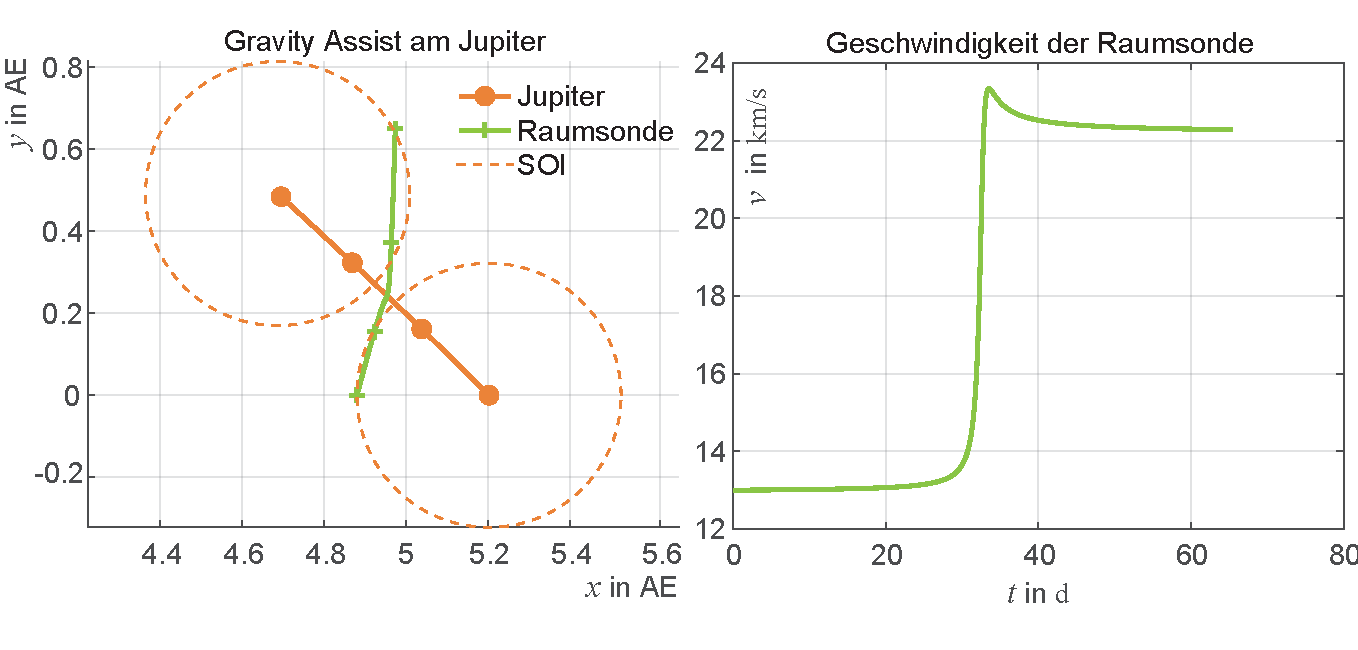
\includegraphics[width=\textwidth]{GravityAssistSimulation.pdf} 
	\caption[Gravity-Assist-Man�ver Simulation.]{Ergebnisse der Gravity-Assist-Man�ver Simulation im heliozentrischen \KOS am Beispiel des Flugs einer Raumsonde um den Jupiter.  Parameter: $v_1 = \SI{13.0}{\km\per\second}$, $\gamma_1 = 75\degree$.}
	\label{abb:adyn_lsgswingby02}
\end{figure}

\end{sol} 
\textcolor{blue} {$\rightarrow$ zur} \probref{adyn_swingby03}.\\
\noindent\rule[1ex]{\textwidth}{0.5pt}  \newpage  \clearpage

%-----------------------------------------------------------------------------------------------------------
\newpage 
\subsection{�bungen zu Rendezvous im Weltall}

\begin{sol}{prob:adyn_rendezvous01}\label{lsg:adyn_rendezvous01} %�bung22
\textbf{Rendezvous ISS und Raumtransporter}\\

Wir wollen zun�chst die Beziehungen \eqref{eq:adyn_rendez23} und \eqref{eq:adyn_rendez24} aus \kap{adyn_rendezvous} herleiten, die wir f�r unsere \matlab-
Programmierung gut verweenden k�nnen. Wir starten von der Darstellung \eqref{eq:adyn_rendez23}:
\begin{nebenrechnungNeu} {Clohessy-Wiltshire-Gleichungen}
\begin{align}
\begin{split}
    \omega\,x &= \lk 6 \omega\, y_0 + 4\dot{x}_0\rk\,  \sin \omega t + 2 \dot{y}_0 \, \cos \omega t + \omega t \, \lk -6 \omega\,  y_0 - 3 \dot{x}_0\rk  + \omega\,  \lk x_0 - 2 \dot{y}_0\rk\,,  \\
    \omega \, y &= \lk \dot{y}_0\rk \,  \sin \omega t + \lk -3 \omega \, y_0 - 2 \dot{x}_0\rk \,  \cos \omega t + \omega \, \lk 4 y_0 + 2 \dot{x}_0\rk  \, ,\\
    \omega \, z &= \dot{z}_0\, \sin \omega t + \omega\,  z_0 \, \cos \omega t +0
\end{split}\label{eq:adyn_CWEq_01}
\end{align}

Umordnung nach $\dot{x}_0, \dot{y}_0, \dot{z}_0$ und $x = y = z = 0$:

\begin{align}
\begin{split}
    \begin{pmatrix} 0 \\ 0 \\ 0 \end{pmatrix} =\,
    &\underbrace{\begin{pmatrix} 4 \sin \omega t - 3 \omega t & 2 \cos \omega t - 2 & 0 \\
    -2 \cos \omega t + 2 & \sin \omega t & 0 \\
    0 & 0 & \sin \omega t 
    \end{pmatrix} }_{\substack{\hat{A}}}
    \begin{pmatrix} \dot{x}_0 \\ \dot{y}_0 \\ \dot{z}_0 \end{pmatrix} 
    \\ &+ \underbrace{\begin{pmatrix} 6 \omega \,y_0\, \sin \omega t - 6 \omega^2 t\,y_0 + \omega x_0 \\
    -3 \omega \,y_0\, \cos \omega t + 4 \omega\, y_0 \\
    \omega\, z_0\, \cos \omega t 
    \end{pmatrix}}_{\substack{-\hat{B}}}
\end{split}\label{eq:adyn_CWEq_02}
\end{align}
\begin{align}
    -\hat{B} &= \omega \, 
    \begin{pmatrix}
        6 y_0\,\sin \omega t - 6 \omega t \,y_0 + x_0 \\ 
        -3 y_0\, \cos \omega t + 4 y_0 \\ 
        z_0\, \cos \omega t 
    \end{pmatrix} \label{eq:adyn_CWEq_03}\\
    \rightarrow \quad \hat{B} &= \omega \,
    \begin{pmatrix}
        -6 y_0 \,\sin \omega t + 6 \omega t\, y_0 - x_0 \\ 
        3 y_0\, \cos \omega t - 4 y_0 \\ 
        -z_0\, \cos \omega t 
    \end{pmatrix} \label{eq:adyn_CWEq_04}\\
  \rightarrow\quad  \hat{B} &=      \hat{A} \hat{X}\nonumber\\
    \rightarrow\quad \hat{X} &= 
    \begin{pmatrix} 
        \dot{x}_0 \\ 
        \dot{y}_0 \\ 
        \dot{z}_0 
    \end{pmatrix} 
    = \hat{A}^{-1}\, B\label{eq:adyn_CWEq_05}
\end{align}
\subsubsection*{Cramersche Regel}
\begin{align}
    \dot{x}_0 &= \frac{\det \hat{A}_x}{\det \hat{A}}, \quad
    \dot{y}_0 = \frac{\det \hat{A}_y}{\det \hat{A}}, \quad
    \dot{z}_0 = \frac{\det \hat{A}_z}{\det \hat{A}}\label{eq:adyn_CWEq_06}
\end{align}
\begin{align}
    \det \hat{A} &= 
    \begin{vmatrix}
        \lk 4 \sin \omega t - 3 \omega t \rk & -2\, \lk 1 - \cos \omega t \rk & 0 \\
        +2 \,\lk 1 - \cos \omega t \rk & \sin \omega t & 0 \\
        0 & 0 & \sin \omega t
    \end{vmatrix} \label{eq:adyn_CWEq_07}
\end{align}
\begin{align*}
    &= \lk 4 \sin \omega t - 3 \omega t \rk\, \sin^2 \omega t + 4 \sin \omega t \,\lk 1 - \cos \omega t \rk^2\\
    &= \sin \omega t \,
    \lk 4 \sin^2 \omega t - 3 \omega t \,\sin \omega t + 4 + 4 \cos^2 \omega t - 8 \cos \omega t \rk\\
    &= \sin \omega t \,
    \lek 8 \,\lk 1 - \cos \omega t \rk - 3 \omega t\, \sin \omega t \rek
\end{align*}
\begin{align}
    \det \hat{A}_z &=
    \begin{vmatrix}
         4 \sin \omega t - 3 \omega t & -2 \,\lk 1 - \cos \omega t \rk & -6 \omega \,y_0\, \sin \omega t + 6 \omega^2 t\, y_0 - \omega \,x_0 \\
        2 \,\lk 1 - \cos \omega t \rk & \sin \omega t & -3 \omega \,y_0\, \cos \omega t - 4 \omega \,y_0 \\
        0 & 0 & -\omega \,z_0\, \cos \omega t
    \end{vmatrix}\\
    &= -\lk 4 \sin \omega t - 3 \omega t \rk \,\sin \omega t \,\omega \,z_0 \,\cos \omega t - 4 \omega \,z_0 \,\cos \omega t \,\lk 1 - \cos \omega t \rk^2\nonumber\\
    &= -\cos \omega t \,\omega \,z_0 \,
    \lk 4 \sin^2 \omega t - 3 \omega t \,\sin \omega t + 4 + 4 \cos^2 \omega t - 8 \cos \omega t \rk \nonumber\\
    &= -\cos \omega t \,\omega \,z_0 \,
    \lek 8 \,\lk 1 - \cos \omega t \rk - 3 \omega t \,\sin \omega t \rek \nonumber\\
    \rightarrow \quad \dot{z}_0 &= - \frac{\cos \omega t\, \omega\, z_0}{\sin\omega t} = -\frac{\omega\,z_0}{\tan\omega t}\label{eq:adyn_CWEq_09}
\end{align}
\begin{align}
    \det \hat{A}_x &=
    \begin{vmatrix}
        6 \omega \,y_0\, \sin \omega t - 6 \omega^2 \,t \,y_0 + \omega \,x_0 & -2 \,\lk 1 - \cos \omega t \rk & 0 \\
        -3 \omega\, y_0\, \cos \omega t + 4 \omega\, y_0 & \sin \omega t & 0 \\
        \omega\, z_0\, \cos \omega t & 0 & \sin \omega t
    \end{vmatrix}\label{eq:adyn_CWEq_10}
\end{align}
\medskip

\end{nebenrechnungNeu}
%%%%%%%%%%%%%%%%%%%%%%%%%%%%%%%%%%%%%%%%%%%%%%%%%%%%%%%%%%%%%%%%%%%%%%%%%%%%%%%%%%%%%%%%%%%
%
%%BEISPIEL 1 %%%%%%%%%%%%%%%%%%%%%%%%%%%%%%%%%%%%%%%%%%%%%%%%%%%%%%%%%%%%%%%%%%%%%%%%%%%%%%%%%
%\begin{example}{R�ckkehr eines Astronauten zur Raumstation}  
%Wir nehmen folgende Parameter an: 
%\begin{align*}
    %h_\text{ISS} &= \SI{420.0}{\km}\,, ~ R_0 = \SI{6778}{\km} \,,~
    %T_\text{P}   = \SI{ 92.4}{\min}\,, ~ \omega_0 = \SI{1.13e-3}{\radian\per\second}\,,~  x_0' = y_0' = \SI{100}{\metre}\,, ~\dot{x}_0' = \dot{y}_0' = 0\,.
%\end{align*}
%\begin{enumerate}
    %\item [a)]
    %Was passiert, wenn der Astronaut \anf{nichts} macht?
    %\begin{align}
        %x'\lk t\rk &= x_0'-6\,y_0'\,\lek\omega_0 t - \sin\lk\omega_0 t\rk\rek\,, ~~~ y'\lk t\rk = y_0' +3\,y_0'\,\lek 1-\cos\lk\omega_0t\rk\rek\,. \label{eq:adyn_rendez26}
    %\end{align}
    %Der Astronaut wird sich durch die Gezeitenkraft in $x'$-Richtung immer weiter von der ISS entfernen und dabei durch die Coriolis-Kraft in $y'$-Richtung eine Art schwingende Bewegung ausf�hren (\figref{adyn_rendezvous02}).
		%
	%\begin{figure}[H]
	%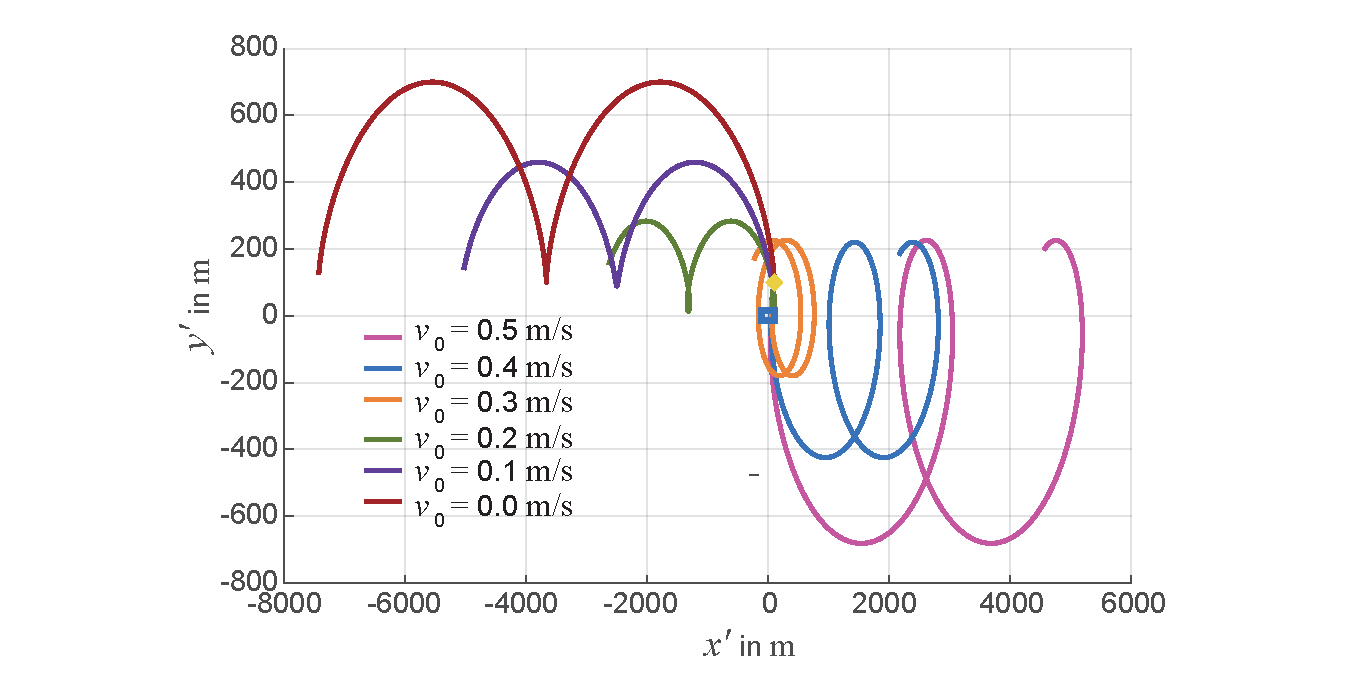
\includegraphics[width=\textwidth]{RendezvousAstronaut01.pdf} 
	%\caption[Astronaut au�erhalb der ISS.]{Astronaut au�erhalb der ISS. Der Astronaut befindet sich initial bei $x_0'=y_0'=\SI{100}{\metre}$ und bewegt sich mit einer Anfangsgeschwindigkeit $v_0$ (also keine initiale Relativgeschwindigkeit zum Ziel, d.h. $\dot{x}_0'=\dot{y}_0=0'$) genau in Richtung auf die Station zu. Selbst bei $v_0=0$ entfernt sich der Astronaut mit der Zeit von der Raumstation. Dargestellt sind die L�sungen der Clohessy-Wiltshire-Gleichungen wie im \mscr~ \mladynref{Rendezvous01.m} im Detail ausgef�hrt.}
	%\label{abb:adyn_rendezvous02}
%\end{figure}
%
  %\item[b)]
    %Was passiert, wenn der Astronaut seinen R�ckkehrantrieb (englisch \textit{Return-Thruster}) mit einem Antriebsverm�gen von $\SI{1}{\metre\per\second}$ einsetzt?   
		%Intuitiv \anf{zielt} der Astronaut mit seinem auf dem R�cksto�-Prinzip basierenden Thruster genau in Richtung ISS, also mit
    %\begin{align*}
        %\vec{v}_0 = 
        %\begin{pmatrix}
            %\dot{x}_0'\\
            %\dot{y}_0'\\
            %\dot{z}_0'
        %\end{pmatrix}
        %= \frac{1}{\sqrt{2}}
        %\begin{pmatrix}
            %1\\
            %1\\
            %0
        %\end{pmatrix}
        %\SI{}{\metre\per\second}\,.
    %\end{align*}
    %Leider wird durch die kombinierte Wirkung der Gezeiten und Coriolis-Kraft der Astronaut die ISS verfehlen, wie Gleichung \eqref{eq:adyn_rendez23} und \figref{adyn_rendezvous02} und \figref{adyn_rendezvous03}a zeigen.\\
    %\item[c)]
    %Wie muss der Astronaut beim Abfeuern seines Thrusters zielen, damit er die ISS sicher erreicht? \\
		%$\dot{x}_0'$, $\dot{y}_0'$ ergeben sich aus \eqref{eq:adyn_rendez24}. Wir k�nnen noch eine kleine Eigengeschwindigkeit des Astronauten vor dem Starten des Thrusters mit $\vec{v}_\text{vor} = \lk\dot{x}_{\text{vor},0'}, \dot{y}_{\text{vor},0'}\rk$ annehmen und erhalten den richtigen Zielwinkel:
    %\begin{align}
        %\tan\lk\gamma\rk = \frac{\Delta v_y}{\Delta v_x} = \frac{\dot{y}_0' -\dot{y}_{\text{vor},0'}}{\dot{x}_0'- \dot{x}_{\text{vor},0'}} \,. \label{eq:adyn_rendez27}
    %\end{align}
%\end{enumerate}
%In der Realit�t wird sich der Astronaut nat�rlich in kleinen Minisch�ben iterativ der ISS n�hern, doch auch daf�r gelten die abgeleiteten Formeln.
%
%\begin{figure}[H]
	%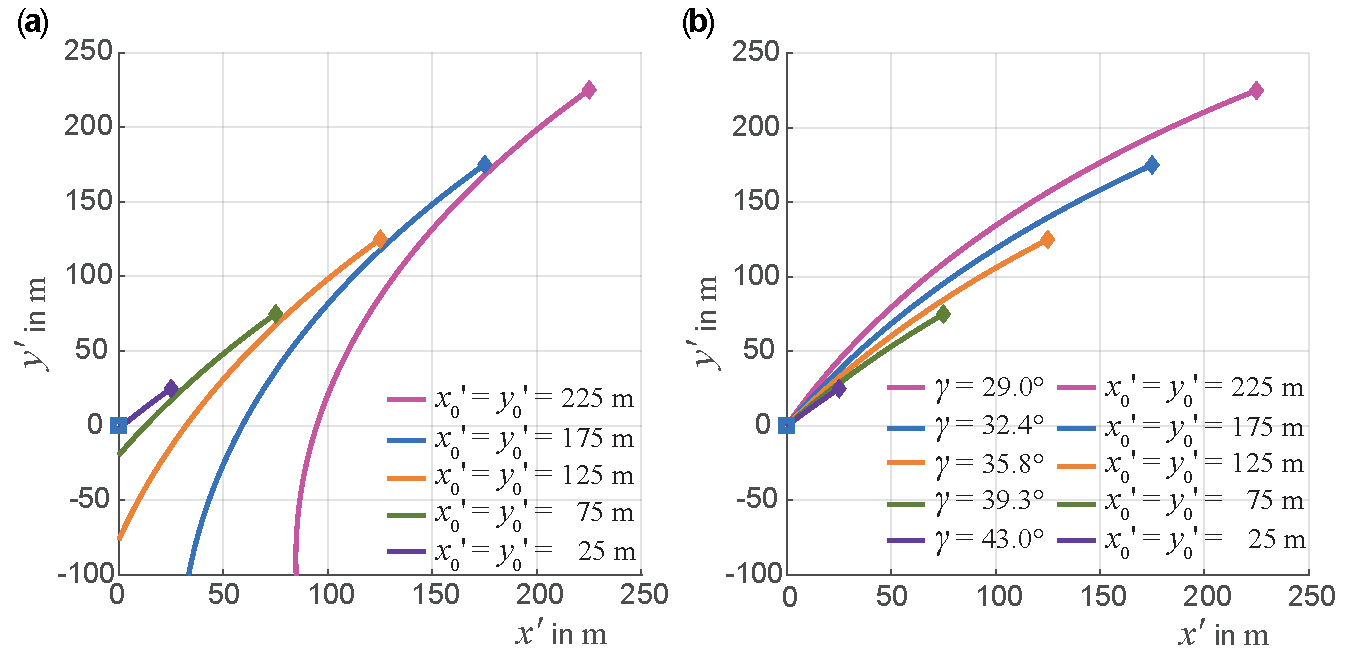
\includegraphics[width=\textwidth]{RendezvousAstronaut02.pdf} 
	%\caption[Astronaut au�erhalb der ISS.]{Astronaut au�erhalb der ISS. \fa Der Astronaut befindet sich initial bei $x_0'=y_0'=\SI{25}{\metre} \ldots \SI{225}{\metre}$ und "`zielt"' mit seinem Antriebssystem  mit einer Anfangsgeschwindigkeit $v_0$ genau in Richtung auf die Station. L�sung der Hill-Gleichungen. \fb Der Astronaut befindet sich ebenfalls initial bei $x_0'=y_0'=\SI{25}{\metre} \ldots \SI{225}{\metre}$ und bewegt sich mit einem optimierten Zielwinkel $\gamma$ der Richtung Anfangsgeschwindigkeit von $v_0 = \SI{1}{\metre\per\second}$ auf die Station zu (L�sung der Clohessy-Wiltshire-Gleichungen\index{Clohessy-Wiltshire-Gleichungen}). Offensichtlich wird der Astronaut erst bei Entfernung von kleiner als 50 m bei direkter Anzielung der Station auch bei dieser wirklich ankommen. Die Rechnungen sind im \mscr~ \mladynref{Rendezvous02.m} im Detail ausgef�hrt.}
	%\label{abb:adyn_rendezvous03}
%\end{figure}
%
%\label{bsp:adyn_stranded_astronaut}
%\end{example}
%
%

Wir verweisen auf die MATLAB-Skripte \mladynref{Rendezvous04.m} und \mladynref{Rendezvous05.m}.

\begin{figure}[H]
	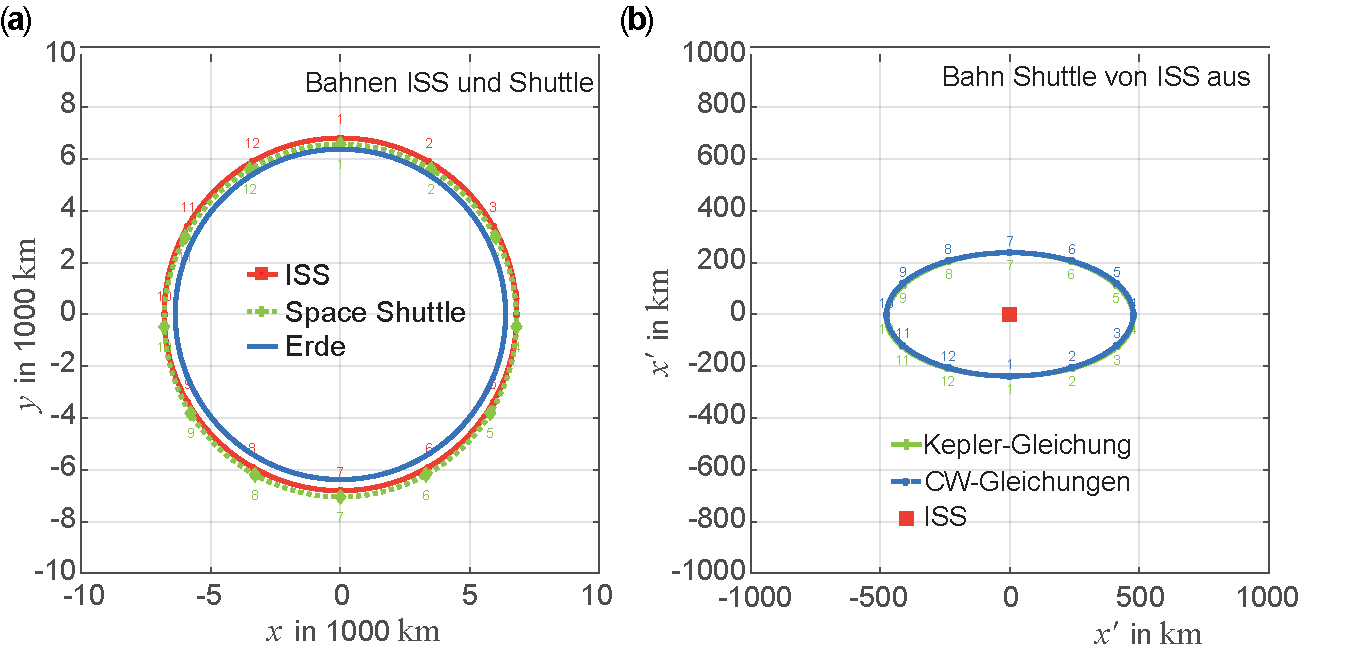
\includegraphics[width=\textwidth]{SpaceShuttle2ISS.pdf} 
	\caption[Space Shuttle und ISS in unterschiedlichen Umlaufbahnen.]{Space Shuttle und ISS in unterschiedlichen Umlaufbahnen. \fa Bahnen von ISS und Space Shuttle. Die Shuttle Bahn ist fiktiv, um das Prinzip zu erl�utern. In der Realit�t war die Shuttle Bahn viel n�her an der ISS. \fb Bahn Space Shuttle von ISS aus. L�sungen nach der Kepler-Gleichung mit Drehung des mitbewegten \KOS des Ziels und CW-L�sung im Vergleich. Die �bereinstimmung der exakten L�sungen nach der Kepler-Gleichung mit der CW-L�sung ist sehr gut, da auf Grund der Parameter die Linearisierungsbedingung f�r die CW-Gleichung relativ gut erf�llt ist.}
	\label{abb:adyn_rendezvous04Lsg}
\end{figure}

\end{sol} 
\textcolor{blue} {$\rightarrow$ zur} \probref{adyn_rendezvous01}.\\
\noindent\rule[1ex]{\textwidth}{0.5pt}  \newpage  \clearpage


%-----------------------------------------------------------------------------------------------------------

\begin{sol}{prob:adyn_rendezvous02}\label{lsg:adyn_rendezvous02} %�bung23
\textbf{Rendezvous Apollo 11 CSM und LM}\\

Die L�sung zum Rendezvous von LM und CSM von Apollo 11 in der Mondumlaufbahn ist im Detail im \mscr~\mladynref{LMCSMApollo11.m} als Berechnung der Kinematik des Rendezvous �ber die Clohessy-Wiltshire-Gleichungen ausgef�hrt. Wir erhalten die \figref{adyn_rendezvous06} aus \kap{adyn_rendezvous_apollo11}.\\

\begin{figure}[H]
	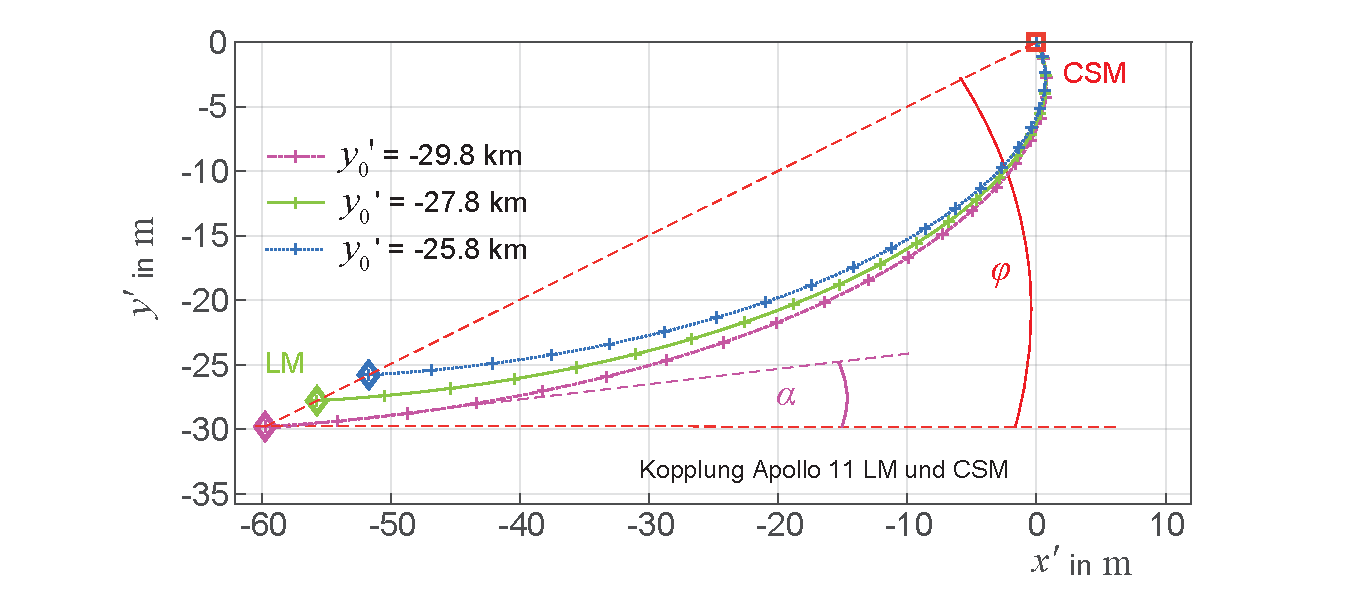
\includegraphics[width=\textwidth]{Apollo11LMCSMTrajektorie.pdf} 
	\caption[Trajektorien des LM im Anflug auf das CSM von Apollo 11.]{Trajektorien des LM im Anflug auf das CSM von Apollo 11 f�r verschiedene H�hen des TPI-Burn. Siehe \probref{adyn_rendezvous02} \bzw \mscr{}\mladynref{LMCSMApollo11.m}.}
	\label{abb:adyn_rendezvous06_uebung}
\end{figure}

\end{sol} 
\textcolor{blue} {$\rightarrow$ zur} \probref{adyn_rendezvous02}.\\
\noindent\rule[1ex]{\textwidth}{0.5pt} \newpage \clearpage 

%-----------------------------------------------------------------------------------------------------------

\begin{sol}{prob:adyn_rendezvous03}\label{lsg:adyn_rendezvous03} %�bung24
\textbf{Planung einer Apollo Mission - \textit{Free Return Trajectory}}\\

\begin{subprobs}
\subprob{Absch�tzungen}
Wir wollen als erstes eine Absch�tzung f�r die Flugzeit zum Mond treffen und nehmen dabei eine koplanare Bewegung von Flugbahn und Mondbahn an, letztere wird auch noch als Kreisbahn angenommen (\figref{adyn_FRT01}).\\
Der Punkt $\mathrm{P}_0$ (Abstand $r_0$ vom Erdzentrum) in der Parkbahn um die Erde, aus der der Einschuss (Injektion) in die translunare Bahn erfolgt, wird \textit{(Translunar Injection Point} (TLI) genannt. Dort gilt f�r die Energie und den Drehimpuls des Raumschiffs bezogen auf das Erd-\KOS:
\begin{align}
H_0 = \frac{v_0{}^2}{2} - \frac{\mu_\text{E}}{r_0}\,, & L_0 = r_0\,v_0\,\cos\gamma_0\,. \label{eq:adyn_lsg_FRT01}
\end{align}
Hierin sind $v_0\,\cos\gamma_0$ die Komponente der Raumschiff-Geschwindigkeit in Richtung lokaler Horizont mit $\gamma_0$ als der FPA bei $r_0$.\\
Damit ergeben sich f�r die Ellipse zum Mond folgende Ellipsenparameter (vergleiche auch Gleichungen \eqref{eq:hm_bewgl1} und \eqref{eq:hm_relations1}):
\begin{align}
\begin{split}
    p &= \frac{L_0{}^2}{\mu_ \text{E}}\,,~~~~ a = -\frac{\mu_\text{E}}{2H_0}\,, ~~~~
    e = \sqrt{1 - \frac{p}{a}} \,=\, \sqrt{1+\frac{L_0{}^2}{\mu_\text{E}{}^2}\,2H_0}\,~.
\end{split} \label{eq:adyn_lsg_FRT02}
\end{align}
\begin{figure}[H]
	\includegraphics[width=\textwidth]{Transfer2Moon.pdf} 
	\caption[Geometrie des Flugs zum Mond.]{Vereinfachte Geometrie des Flugs eines Raumschiffes zum Mond. Im Bild wurde eine koplanare Bewegung von Raumschiff und Mond in der Ekliptik angenommen (Draufsicht auf die Ekliptik). (Nach \cite{Bate1971}).}
	\label{abb:adyn_FRT01}
\end{figure}

In \figref{adyn_FRT01} definieren wir aus der Geometrie f�r die weitere mathematische Behandlung folgende Parameter:
\begin{align*} 
    r_0 && &\text{geozentrischer Abstand des Raumschiffs bei Injektion in die translunare Bahn} \\
    r_1 && &\text{geozentrischer Abstand des Raumschiffs beim Erreichen der SOI des Mondes}\\
    && &r_1 = \sqrt{r_{\text{EM}}{}^2 + R_{\text{SOI, M}}{}^2 - 2 r_{\text{EM}} R_{\text{SOI, M}} \cos\gamma_1} \\
    r_\text{EM} && &\text{Abstand der Massezentren von Erde und Mond}      \\
    R_\text{SOI,M} && &\text{Radius der SOI des Mondes}\\
    \varphi_0 && &\text{geozentrischer Phasenwinkel des Mondes bei Abflug (TLI) relativ zur}\\
    && &\text{Verbindungslinie Erde/Raumschiff}\\
    \varphi_1 && &\text{geozentrischer Phasenwinkel des Mondes bei Ankunft des Raumschiffs }\\
    && &\text{an der SOI relativ zur Verbindungslinie Erde/Raumschiff}\\
    \lambda_1 && &\text{selenozentrischer Winkel zwischen Ankunftsort des Raumschiffs}\\
    && &\text{an der SOI des Mondes und der Verbindungslinie Erde/Mond}\\
    \gamma_0,\gamma_1 && &\text{FPA des Raumschiffs bei TLI \bzw Ankunft an der SOI des Mondes}\\
    \upsilon_0,\upsilon_1 && &\text{wahre Anomalien der Ellipsenbahn bei TLI \bzw Ankunft SOI des Mondes}\\
    \omega_\text{M} && &\text{Umlaufgeschwindigkeit des Mondes}\,\approx \SI{2.649e-6}{\radian\per\second}\\
		a, e, P && &\text{Parameter der Transferellipse zum Mond}
\end{align*}
F�r eine Planung eines Fluges zum Mond startet man mit Vorgaben f�r $r_0,\,v_0,\,\gamma_0$ und $\lambda_1$ und berechnet die Flugzeit $t_\text{F} = \mathrm{ToF}$,\;$\varphi_0$,\, $\varphi_1$ und $\gamma_1$. Ergeben sich daraus keine sinnvollen Werte, so muss man $r_0,\,v_0,\,\gamma_0$ und $\lambda_1$ variieren. \\
Aus den Ellipsenparametern $a$, $p$, $e$ lassen sich nun bei bekannten $r_0,r_1$ die jeweiligen wahren Anomalien berechnen.
\begin{align}
\begin{split}
    \cos\upsilon_0 &= \frac{p - r_0}{\e\,r_0} \,,\\
    \cos \upsilon_1 &= \frac{p - r_1}{\e \,r_1} \quad \text{mit} \quad r_1 = \sqrt{r_{\text{EM}}{}^2 + R_{\text{SOI,M}}{}^2 - 2 r_{\text{EM}}\,R_{\text{SOI,M}} \cos \lambda_1}
\end{split}\label{eq:adyn_lsg_FRT03}
\end{align}
Die Flugzeit zum Mond ergibt sich �ber die Kepler-Gleichung zu:
\begin{align}
    t_\text{F} = t_1 - t_0 = \lk\sqrt{\frac{a^3}{\mu_\text{E}}}\rk \lek E_1 - E_0 - \e\,\lk \sin E_1 - \sin E_0\rk\rek\label{eq:adyn_lsg_FRT04}
\end{align}
wobei sich die exzentrische Anomalien $E_i~~(i=1,2)$ entweder aus
\begin{align}
\begin{split}
    \cos E_i &= \frac{\e - \cos \upsilon_i}{1 + \e \cos \upsilon_i} = \lk 1 - \frac{r_i}{a}\rk\,\frac{1}{\e}\\
    \text{oder}\quad \tan \frac{E_i}{2} &= \sqrt{\frac{1-\e}{1+\e}}\,\tan \lk \frac{\upsilon_i}{2} \rk    
\end{split}\label{eq:adyn_lsg_FRT05}
\end{align}
ergeben (\vgl Gleichungen \eqref{eq:hm_r_param_ellipse} und \eqref{eq:hm_nu(t)_alternativ}).\\
Wir brauchen noch den Winkel $\varphi_1$, dieser ergibt sich nach dem Sinussatz aus
\begin{align}
    \sin\varphi_1 = \frac{R_{\text{SOI,M}}}{r_1}\,\sin\lambda_1 \,. \label{eq:adyn_lsg_FRT06}
\end{align}
F�r eine Absch�tzung der Flugzeiten wollen wir annehmen, dass $\gamma_0 \approx 0$ ist. Wir k�nnen dann die Flugzeiten f�r verschiedene $\lambda_1$ \bzw $\varphi_1$ als Funktion der TLI-Geschwindigkeit $v_0$ berechnen.

\begin{figure}[H]
	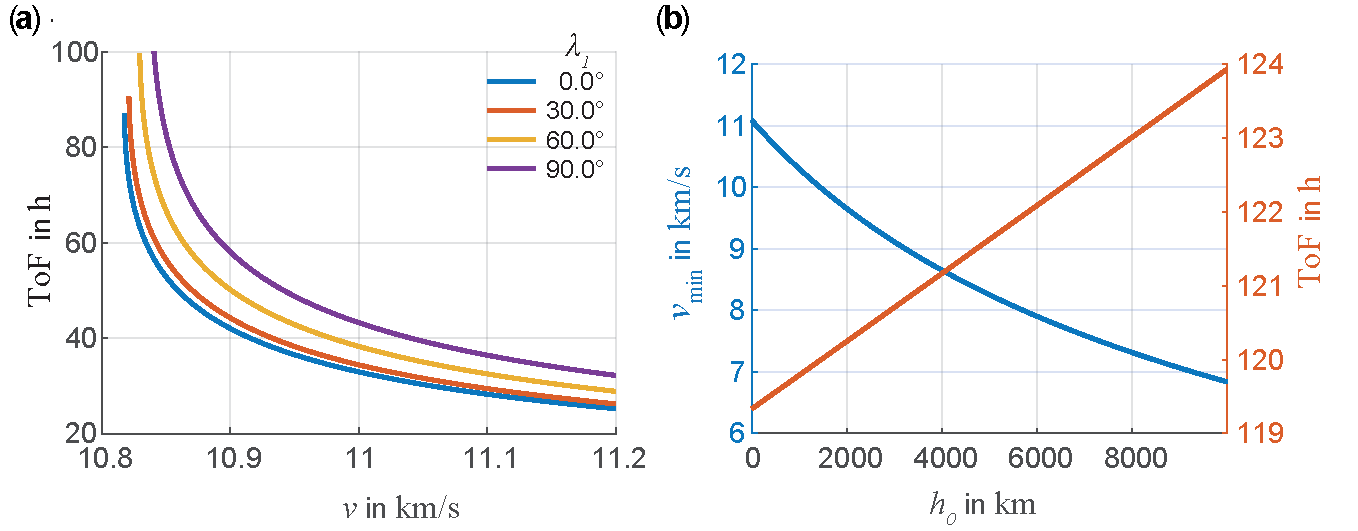
\includegraphics[width=\textwidth]{Transfer2MoonTOF.pdf} 
	\caption[Flugzeiten und Minimalgeschwindigkeit zum Mond.]{Flugzeiten und Minimalgeschwindigkeit zum Mond. \fa ToF als Funktion der TLI-Geschwindigkeit $v_0$ \fb Minimum-Geschwindigkeit $v_\text{min}$ f�r TLI und zugeh�rige ToF als Funktion des Radius $r_0$ der erdnahen Kreisbahn. Siehe \mscr~\mladynref{Transfer2Moon.m}.}
	\label{abb:adyn_FRT02}
\end{figure}

Man erkennt aus \figref{adyn_FRT02}a, dass es eine minimale Geschwindigkeit $v_{\text{min}}$ (abh�ngig vom Winkel $\lambda_1$) gibt, um �berhaupt in endlicher Zeit den Mond zu erreichen. Diese liegt bei etwas �ber $\SI{10.8}{\km\per\second}$ f�r $\lambda_1 =0$ und ist ebenfalls abh�ngig und der H�he $h_0$ der Parkbahn in Erdn�he.\\
Man kann nun eine einfache numerische Absch�tzung f�r $v_{\text{min}}$ machen, wenn man annimmt, dass die TLI am Perig�um erfolgen soll.
Dann ist definitiv $\gamma_0 = 0$ und das Apog�um der elliptischen translunaren Bahn entspricht dann $r_{\text{EM}}$ (\bzw $r_{\text{EM}} - R_{\text{SOI,M}}$, wenn wir die SOI ber�cksichtigen wollen). Wir finden also:
\begin{align}
     2a_0 &= r_0 + r_{\text{EM}} ~~~\text{und}~~~H_0 = -\frac{\mu_\text{E}}{2a} = \frac{v_{\text{min}}{}^2}{2} - \frac{\mu_\text{E}}{r_0} \nonumber \\
    \rightarrow \quad v_{\text{min}}{}^2 &= \frac{2\mu_\text{E}}{r_0}\,\lk 1 - \frac{1}{1 + r_{\text{EM}}/r_0}\rk ~~ \text{und} ~~~ \text{ToF}_{\text{max}} = \pi \sqrt{\frac{a_0{}^3}{\mu_\text{E}}} \,. \label{eq:adyn_lsg_FRT07}
\end{align}
Man erh�lt dann \zb f�r $h_0 = \SI{400}{\km}$ eine minimale notwendige Geschwindigkeit von $v_{\text{min}} = \SI{10.75}{\km\per\second}$ und eine (maximale) Flugzeit von $ \text{ToF}_{\text{max}} = \SI{119.5}{\hour}$ (\figref{adyn_FRT03}), 
was wesentlich l�nger ist, als \zb Apollo 11 zum Mond brauchte.\\
Man erkennt sehr sch�n aus \figref{adyn_FRT02}, wie kleine �nderungen der TLI-Anfangsgeschwindigkeit die Flugzeit wesentlich verk�rzen.

\subprob {\textit{Patch Conic} - N�herung}

Nach diesen grunds�tzlichen �berlegungen wollen wir nun die Bahn genauer berechnen und dabei das Konzept der SOI (siehe \kap{adyn_gravity_assist} \bzw \probref{adyn_SOI}) benutzen. Bisher haben wir ja die Gravitationswirkung des Mondes vernachl�ssigt. Wir arbeiten in den relevanten Bereichen jeweils nur mit der SOI der Erde \bzw des Mondes. Dies f�hrt auf das sogenannte Konzept der \textit{Patched Conic} (der "`aneinandergest�ckelten Kegelschnitte"', \vgl auch \probref{adyn_SOI}). 

\begin{figure}[H]
	\includegraphics[width=\textwidth]{Transfer2MoonPP.pdf} 
	\caption[Geometrie des Transfers zum Mond am \textit{Patch Point}.]{Geometrie des Transfers zum Mond am \textit{Patch Point}. Die Koordinaten im selenozentrischen \KOS werden mit dem Index 2 bezeichnet und sind in rot gezeichnet. Der Winkel $\varepsilon_2$ bezeichnet den anf�nglichen selenozentrischen Winkel der Geschwindigkeit des Raumschiffs relativ zum Mondzentrum. (Nach \cite{Bate1971}.)}
	\label{abb:adyn_FRT03}
\end{figure}

Wir berechnen zun�chst die Transferphase vom TLI bis zum Erreichen der SOI des Mondes. Dazu berechnen wir �ber \eqref{eq:adyn_lsg_FRT03}-\eqref{eq:adyn_lsg_FRT05} die ToF und auch den geozentrischen Phasenwinkel $\varphi_0$, den der Mond bei der TLI haben muss:
\begin{align}
    \varphi_0 = \upsilon_1 - \upsilon_0 - \gamma_1 - \omega_{\text{M}}\,  \lk t_1 - t_0\rk\,. \label{eq:adyn_lsg_FRT08}
\end{align}
Wir schauen uns nun genauer die Bedingungen am sogenannten \textit{Patch Point}, dem Punkt PP an. Wir bestimmen dort zun�chst die Geschwindigkeit $\vec{v}_2$ des Raumschiffs im selenozentrischen (\dh lunaren) \KOS:
\begin{align}
\begin{split}
    \vec{v}_2 &= -\vec{v}_{\text{M}} + \vec{v}_1\\
    v_2 &= \sqrt{v_1{}^2 + v_{\text{M}}{}^2 - 2 v_1\,v_{\text{M}}\,\cos \lk \gamma_1 - \varphi_1\rk} 
\end{split}\label{eq:adyn_lsg_FRT09}
\end{align}
mit
\begin{align*}
    v_{\text{M}} = \omega_{\text{M}}\,r_{\text{EM}} \approx \SI{1.018}{\km\per\second}.
\end{align*}
Ferner gilt am Punkt PP $r_2 = R_{\text{SOI,M}}$ und 
\begin{align}
    \varepsilon_2 = \arcsin \lk\frac{v_\text{M}}{v_2}\,\cos\lambda_1 - \frac{v_1}{v_2}\,\cos\lk \lambda_1 + \varphi_1-\gamma_1\rk\rk \,. \label{eq:adyn_lsg_FRT10}
\end{align}
Letztere Beziehung kann man sich ebenfalls aus \figref{adyn_FRT03} �ber
\begin{align*}
    v_2\,\sin\epsilon_2 = v_{\text{M}}\,\cos \lambda_1 - v_1\,\cos\lk\lambda_1 + \varphi_1 - \gamma_1\rk
\end{align*}
herleiten. F�r eine direkte Landung auf dem Mond muss der Winkel $\varepsilon_2$ logischerweise $0$ sein. 
F�r alle anderen F�lle kann man nun mit den \anf{lunaren} Anfangsbedingungen $r_2$, $v_2$ und $\epsilon_2$ drei m�gliche Trajektorien um den Mond herum unterscheiden:
\begin{enumerate}
    \item [1)] Aufschlag auf den Mond: In diesem Fall ist das Periselenium $r_{\text{P,M}}$ (kleinster Abstand der Bahn vom Mondzentrum) kleiner als der Mondradius $R_{\text{M}}$.
    \item [2)] Mondumlaufbahn, \dh Einschwenken auf eine Mondumlaufbahn durch Abbremsen/Beschleunigen auf die notwendige Umlaufgeschwindigkeit  $v_3$.
    \item [3)] Mondumrundung (\zb als \textit{Free Return Trajektory} (FRT)), wobei besonders das Periselenium und die Bedingungen ($r_3$, $v_3$, $\gamma_3$, $\lambda_3$) beim Verlassen der SOI des Mondes interessant sind, da diese in ma�gebliche die R�ckkehrbahn zur Erde bestimmen.
\end{enumerate}
Wir m�ssen daher als n�chstes das Periselenium $r_\text{P,M}$ berechnen, da wir das ja in jedem der drei F�lle zur Bewertung der Bahn um den Mond brauchen. In der SOI des Mondes gilt im \KOS des Mondes gilt nat�rlich wieder Energie- und Drehimpulserhaltung:
\begin{align}
\begin{split}
    H_2 &= \frac{v_2{}^2}{2} - \frac{\mu_\text{M}}{r_2}\,~~\text{mit}~~ \mu_ \text{M} = G\,M_\text{M} \,\\
		L_2 &=  r_2 \, v_2\,\cos \gamma_2 = r_2\,v_2\,\sin \varepsilon_2 \,, ~~\text{da}~~ \gamma_2 = 90^\degree - \varepsilon_2\,.
\end{split}\label{eq:adyn_lsg_FRT11}
\end{align}
Wie bei der Berechnung der Transferellipse finden wir die Kegelschnittparameter\footnote{Der Kegelschnitt wird \ia eine Hyperbel sein.} f�r die Mondbahn:
\begin{align}
    p_2 = \frac{L^2}{\mu_\text{M}}\,, \quad e_2 = \sqrt{1 + \frac{2 H_2\,L^2}{\mu_\text{M}{}^2}} \label{eq:adyn_lsg_FRT12}
\end{align}
und daraus
\begin{align}
    r_\text{P,M} = \frac{p_2}{1 + \e}\,, \quad v_\text{P,M} = \sqrt{2 \lk H_2 + \frac{\mu_\text{M}}{r_\text{P,M}} \rk} \label{eq:adyn_lsg_FRT13}
\end{align}
Wir wollen als Beispiel durchrechnen:
\begin{align*}
    r_0 &= \SI{300}{\km} + R_\text{E} = \SI{6678}{\km}\,,~~
    v_0 = \SI{10.87}{\km\per\second}\,,~~
    \gamma_0 = 0^\degree\,,~~
    \lambda_1 = 30^\degree\,.
\end{align*}
Ohne weitere Kurskorrekturen wird die geringste Entfernung zur Mondoberfl�che
\begin{align*}
    h_\text{P,M} = r_\text{P,M} - R_\text{M} = r_\text{P,M} - \SI{1737.4}{\km} = \SI{1413.6}{\km}\,.
\end{align*}
Wie bereits erw�hnt, kommt es f�r  $h_\text{P,M} < 0$ zur Landung \bzw zum Aufschlag auf dem Mond, abh�ngig von $v\lk h_\text{M} = 0\rk$ und je nach Verf�gbarkeit von Bremsm�glichkeiten.\\

\begin{figure}[H]
	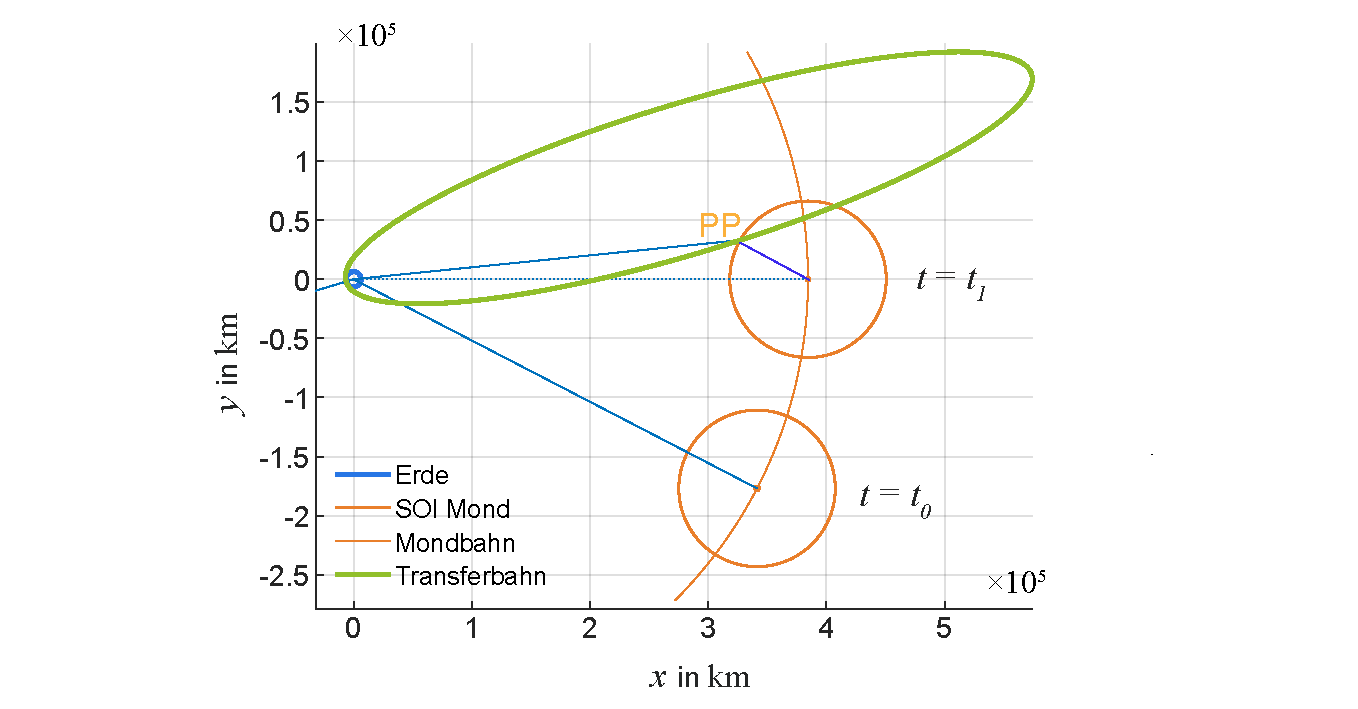
\includegraphics[width=\textwidth]{Transfer2Moon04.pdf} 
	\caption[Berechnete Geometrie des Transfers zum Mond.]{Berechnete Geometrie des Transfers eines Raumschiffes zum Mond. In der Rechnung wurde eine koplanare Bewegung von Raumschiff und Mond in der Ekliptik angenommen. Parameter siehe Tabelle \ref{tab:adyn_FRT01} und \mscr~\mladynref{Transfer2MoonExample.m}.}
	\label{abb:adyn_FRT04}
\end{figure}


Die Parameter f�r die \figref{adyn_FRT04} und \figref{adyn_FRT05} sind in folgender Tabelle gelistet:
\begin{table}[h!]
\centering
\begin{tabular}{|c|c|c|c|c|c|}
\hline
\multicolumn{6}{|l|}{\textbf{Vorgaben und Abflugparameter @TLI}} \\
\hline
$h_0$ (km) & $\gamma_0$ ($\degree$) & $v_0$ (km/s) & $\lambda_1$ ($\degree$) & &   \\
\hline
300.0 & 0.0 & 10.87 & 30.0 & &  \\
\hline
\multicolumn{6}{|l|}{\textbf{Abflugparameter @TLI}} \\
\hline
$a_0$ (km) & $p_0$ (km) & $\e_0$  & $\phi_0$ ($\degree$) &  &  \\
\hline
$\SI{3.03e5}{}$& $\SI{1.32e4}{}$& 0.9780 & 135.77 & &   \\
\hline
\multicolumn{6}{|l|}{\textbf{Parameter auf Transfer zum Mond}} \\
\hline
$v_1$ (km/s) & $v_2$ (km/s) & $\upsilon_1$ &$\upsilon_2$ & $\mathrm{TOF}$ (h) &  \\
\hline
1.054 & 1.220 &0.0 & 5.78 & 50.15&  \\
\hline
\multicolumn{6}{|l|}{\textbf{Parameter am Mond}} \\
\hline
$r_2$ (km) & $\epsilon_2$ ($\degree$) & $p_2$ (km) &$\e_2$ & $h_\text{PM}$ (km)& $\mathrm{TOF}_\text{SOI}$ (h)  \\
\hline
$\SI{6.62e4}{}$ & 4.72 & 9014.8 & 1.8610 & 1413.6 & 28.05 \\
\hline
\end{tabular}
\caption{Parameter f�r \textit{Patch Conic} N�herung} \label{tab:adyn_FRT01}
\end{table}
Hierin ist $\mathrm{TOF}$ die Flugzeit von der TLI bis zum Erreichen der SOI des Mondes und $\mathrm{TOF}_\text{SOI}$ die Flugzeit zum Durchfliegen der SOI des Mondes. \\
Insgesamt ergibt sich f�r einen Flug bis zur R�ckseite des Mondes eine Gesamtflugzeit von
\begin{align*}
    t_\text{F} = \mathrm{TOF} + \frac{1}{2} \mathrm{TOF}_\text{SOI} = \SI{50.15}{\hour} + \SI{14.025}{\hour} \approx \SI{64.175}{\hour}\,,
\end{align*}
also etwa weniger als 3 Tage und damit auch etwas schneller als Apollo 8 unterwegs war.\\

\begin{figure}[H]
	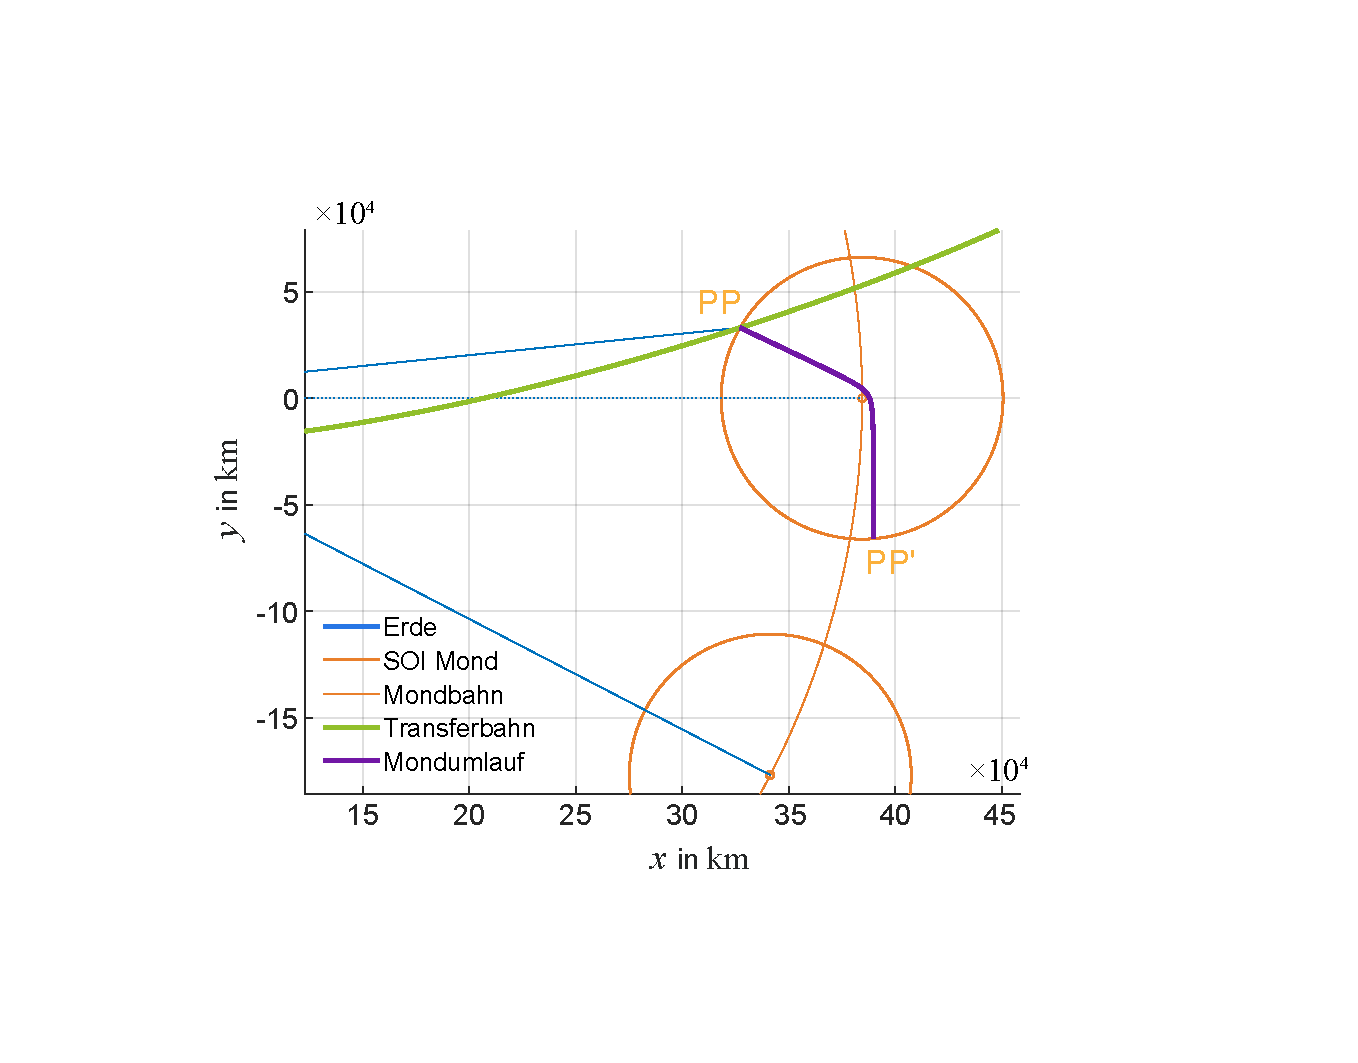
\includegraphics[width=\textwidth]{Transfer2Moon05.pdf} 
	\caption[Berechnete Geometrie des Transfers zum Mond am \textit{Patch Point}.]{Berechnete Geometrie des Transfers zum Mond am \textit{Patch Point}, sowie Mondumlauf. Die lila Kurve zeigt die Bahn des Raumschiffs im \KOS des Mondes. In der Rechnung wurde eine koplanare Bewegung von Raumschiff und Mond in der Ekliptik angenommen. Parameter siehe Tabelle Parameter siehe Tabelle \ref{tab:adyn_FRT01} und \mscr~\mladynref{Transfer2MoonExample.m}. Man beachte, dass \figref{adyn_FRT05} die Bewegung im \KOS des Mondes zeigt und nicht im als Inertialsystem angenommenen geozentrischen \KOS der Erde. F�r eine Energie $H_2 > 0$ wird $\e_2 > 1$ und damit die Bewegung um den Mond eine Hyperbel. Man �berlege sich Analogien zur Behandlung des Gravity-Assist-Man�vers in \kap{adyn_gravity_assist}.}
	\label{abb:adyn_FRT05}
\end{figure}

Man kann die Werte am Punkt PP' berechnen und dann weiter transformieren in das Erd-\KOS, um zu sehen, ob eine \textit{Free Return Trajectory} vorliegt, ganz analog wie beim Swing-By-Man�ver.\\
Wir wollen jedoch im Folgenden die Rechnungen komplett, also auch die Bewegung um den Mond herum im Inertialsystem numerisch machen und k�nnen dabei als Startwert die Parameter der \textit{Patch Conic}-Rechnung �bernehmen.

\newpage
\subprob{Numerische Rechnung Vergleich \textit{Patch Conic} und 1. N�herung}

Wir wollen nun konkret den Raumflug von Apollo 13 anschauen und w�hlen  entsprechend des NASA Flight Journal (\url{https://www.nasa.gov/history/afj/ap13fj/index.html}) $h_0=\SI{169.609}{\km}$. Ebenso benutzen die Ergebnisse der \textit{Patch Conic} N�herung (\figref{adyn_FRT06}) als Startwerte f�r die numerische Rechnung und betrachten zun�chst die Erde als ruhend und den Mond auf einer Kreisbahn umlaufend. 

\begin{figure}[H]
	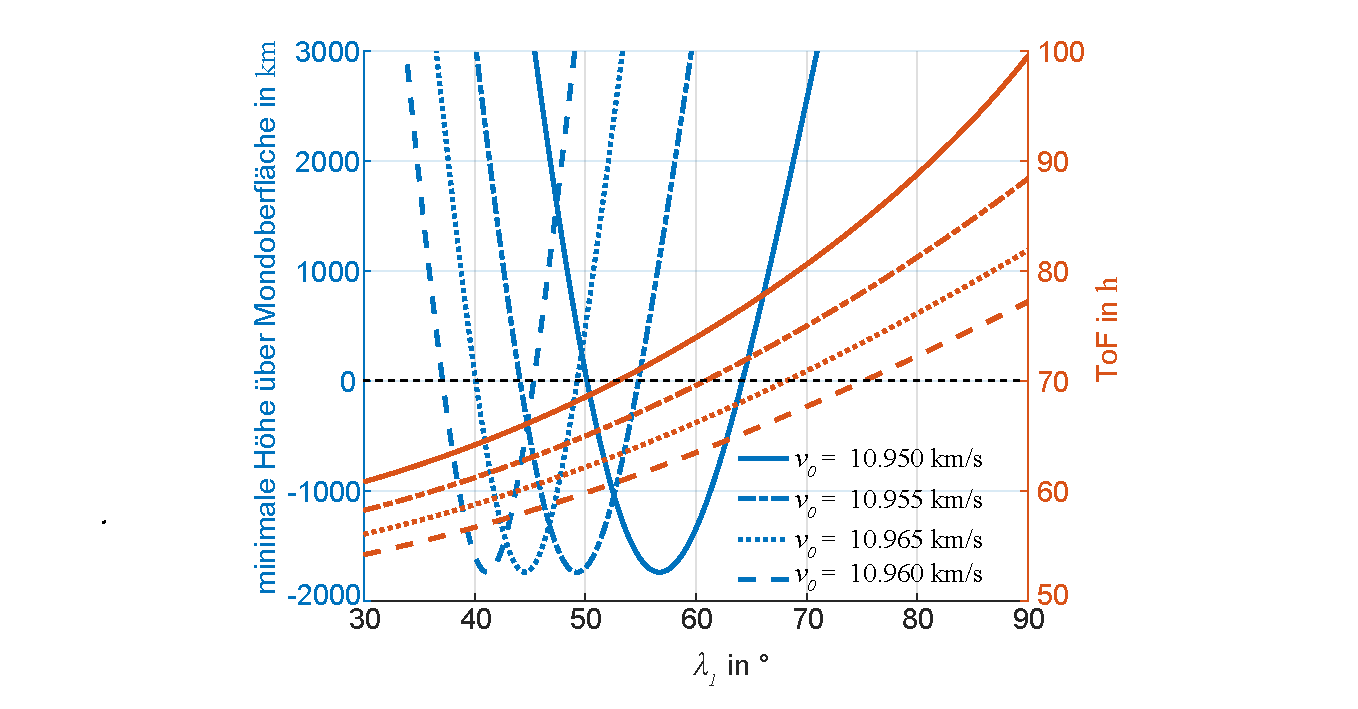
\includegraphics[width=\textwidth]{PatchConicApollo13.pdf} 
	\caption[Ergebnisse der \textit{Patch Conic} N�herung f�r Apollo 13.]{Ergebnisse der \textit{Patch Conic} N�herung f�r Apollo 13.}
	\label{abb:adyn_FRT06}
\end{figure}

Wir erhalten dann \zb f�r $v_0 = \SI{10960.0}{\km\per\second}$ in der
\textit{Patch Conic} N�herung:\\
\begin{align*}
	\lambda_1      &: 49.70\degree  && \\ 
	\varphi_0      &: 129.89\degree\\ 
	\mathrm{ToF} &: 78.7\,\mathrm{h}\\ 
	h_\text{P,M} &: \SI{279.3}{\km} \, 
\end{align*}
was schon relativ gut mit den tats�chlichen Werten von Apollo 13 �bereinstimmt, wobei man ber�cksichtigen muss, dass beim tats�chlichen Raumflug es eine Reihe von Kurskorrekturen gab.

In der numerische Betrachtung (L�sung der Bewegungsgleichungen) ergeben sich dann eine Vielzahl von L�sungen. Das liegt daran, dass es sich bei der Bestimmung der FRT ja um ein Optimierungsproblem handelt, bei dem $h_0$, $h_\text{Reentry}$ und $h_\text{P,M}$ gegeben sind und $v_0$ und $\varphi_0$ gesucht werden. F�r solche Optimierungsprobleme gibt es h�ufig keine eindeutigen L�sungen. Wir erhalten \zb f�r $v_0 = \SI{10960.0}{\km\per\second}$ und $\varphi_0 = 129.33\degree$:
\begin{align*}
	\mathrm{ToF}\, \text{zum Mond} &: 78.2\,\mathrm{h}\\ 
	\mathrm{ToF}\, \text{Gesamt} &: 156.4\,\mathrm{h}\\ 
	h_\text{M,P}\, \text{Mond} &: \SI{2111.0}{\km}\\
	h_\text{Reentry}\, \text{Erde} &: \SI{150.0}{\km} 
\end{align*}
Die L�sung ist im Detail im \mscr~\mladynref{FreeReturnTrajectoryApollo13.m} ausgef�hrt.\\

\subprob{Genauere Rechnungen f�r Apollo 13}

Bisher haben wir die Erde als ruhend angenommen und den Mond auf einer Kreisbahn um diese rotierend, Wir betrachten nun das vollst�ndige Dreik�rper-Problem Erde, Mond und Apollo 13 im Schwerpunktsystem von Erde-Mond. Wiederum handelt sich hierbei um ein Optimierungsproblem, bei dem $h_0$ und $h_\text{Reentry}$ gegeben sein sollen und $v_0$, $\varphi_0$ und $h_\text{P,M}$ gesucht werden.
Die Rechnungen ergeben in diesem Fall beispielhaft, 
\begin{align*}
	v_0      &: \SI{10963.0}{\km\per\second}\\ 
	\varphi_0      &: 130.46\degree\\ 
	\mathrm{ToF}\, \text{zum Mond} &: 75.2\,\mathrm{h}\\ 
	\mathrm{ToF}\, \text{Gesamt} &: 149.5\,\mathrm{h}\\ 
	h_\text{P,M}\, \text{Mond} &: \SI{1353.4}{\km}\\
	h_\text{Reentry}\, \text{Erde} &: \SI{169.6}{\km} \,,
\end{align*}
wobei wir hier vor darauf geachtet haben, dass der Wiedereintritt in die Erdatmosph�re gew�hrleistet ist, daf�r der Mondabstand etwas gr��er gew�hlt ist.
Das L�sungsbeispiel ist in \figref{adyn_FRT08} dargestellt und im Detail im \mscr~\mladynref{FreeReturnTrajectoryApollo13CoM.m} ausgef�hrt.\\

\begin{figure}[H]
	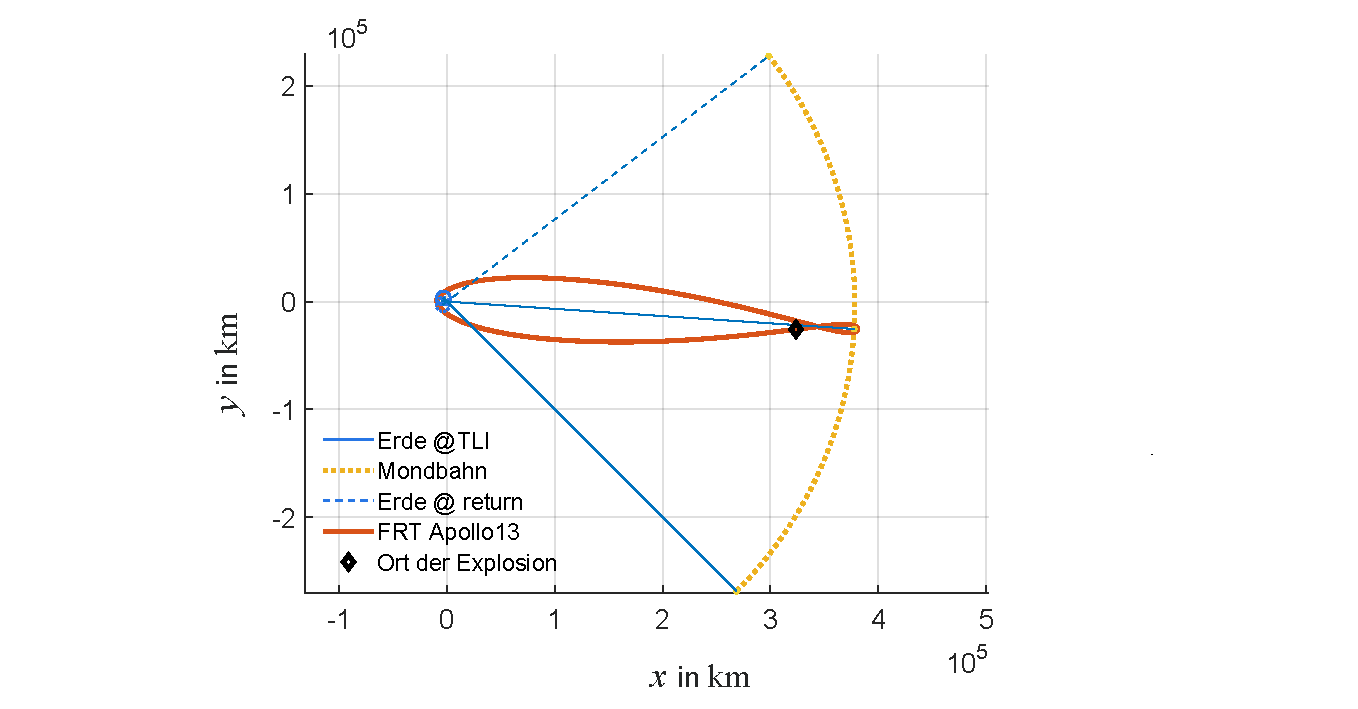
\includegraphics[width=\textwidth]{FRTApollo13.pdf} 
	\caption[Ergebnisse der numerischen Rechnung f�r eine \textit{Free Return Trajectory } f�r Apollo 13.]{Ergebnisse der numerischen Rechnung f�r eine \textit{Free Return Trajectory} im Schwerpunktsystem Erde-Mond. In der Graphik ist auch der Ort der Explosion des Tanksystems von Apollo 13 eingezeichnet.}
	\label{abb:adyn_FRT08}
\end{figure}

\newpage	
\subprob{Allgemeine Bemerkungen - Alternative Ans�tze}

Wie bereits erw�hnt, handelt es sich bei der Bestimmung der FRT um ein Optimierungsproblem. \cite{Battin1999, Brown2002, Bate1971, Vallado2007}. 
Bei der L�sung desselben findet man, dass die L�sungswerte $h_\text{P,M},\, h_\text{Reentry}$ sehr stark auf kleinere Ver�nderungen der Eingabeparameter variieren, \zb wird bei kleinsten �nderungen der Anfangsgeschwindigkeit (TLI-Geschwindigkeit) $v_0$ oder des TLI-Phasenwinkels $\varphi_0$ bei ansonsten festgehaltenen Parametern die Reentry-Flugbahn sehr stark variieren, was bedeuten k�nnte, dass das Raumschiff auf der FRT entweder in der Erdatmosph�re vergl�ht oder von dieser abprallt (siehe \kap{adyn_reentry}).\\
In der Realit�t wird man deswegen die Missionsplanung im Verlauf einer FRT mit kleineren Kurskorrekturen versehen, die wesentliche gr��ere Toleranzen der Parameter ($v_0$, $\varphi_0$) erlauben. Man kann in diesem Fall auch als weitere Randbedingung f�r die Optimierungsaufgabe einen minimalen Treibstoffverbrauch f�r die Summe der einzelnen Kurskorrekturen und Bahn�nderungen fordern, also f�r
\begin{align*}
    \Delta v_{\text{ges}} = \Delta v_{\text{TLI}} + \Delta_\text{Cor,E$\to$M} + \Delta v_{\text{LOI}} + \Delta v_{\text{TEI}} + \Delta_\text{Cor,M$\to$E} + \Delta v_{\text{EOI}}
\end{align*}
Hierbei bedeuten:
\begin{align*}
    \Delta_\text{Cor,E$\to$M} &: \text{Geschwindigkeitsbudget f�r Kurskorrektur auf dem We g $E \to M$ (\bzw $M \to E$)}\\
    \Delta v_\text{LOI,EOI} &: \text{Geschwindigkeitsbudget f�r Lunar Orbit Injektion \bzw Earth Orbit Injektion}\\
    \Delta v_{\text{TEI}} &: \text{Geschwindigkeitsbudget f�r Trans Earth Injektion}
\end{align*}
Dem interessierten Leser sei auf die Ref. \cite{Gagg2016} verwiesen, in welcher auch die einzelnen Schritte der mathematischen Optimierung\footnote{Die Optimierungsprobleme sind generell interessante mathematische Probleme, deren allgemeine Behandlung �ber den Umfang dieses Buches hinaus geht. Wir sind bereits bei der Herleitung der Lagrange-Gleichungen in Band I auf ein Problem dieser Art gesto�en und beim Lambert-Problem.} erl�utert sind.\\
Ebenso verweisen wir auf die unter \url{https://de.mathworks.com/matlabcentral/fileexchange} aufgef�hrten Programme  mit verschiedenen Optimierungsprozeduren in zum Teil vereinfachten Geometrien f�r die Berechnung der FRT.\footnote{ Wir verweisen insbesondere auf:\\
\url{Lunar Free-Return Trajectory Analysis with MATLAB - OTB - File Exchange - MATLAB Central (mathworks.com)},\\ \url{Lunar Free-Return Trajectory Analysis with MATLAB - File Exchange - MATLAB Central (mathworks.com)} und \\
\url{N-body Lunar Free Return Trajectory Analysis � OTB - File Exchange - MATLAB Central (mathworks.com)}.} \\

Wir wollen jedoch noch einen anderen Bezug herstellen. In Kap. 1.2.3.6 in Band I hatten wir das Drei-K�rper-Problem und insbesondere auch das sogenannte eingeschr�nkte Drei-K�rper-Problem eingef�hrt, bei welchem eine dritte Testmasse deutlich kleiner ist als die beiden anderen Massen. Bei dem FRT-Problem handelt es sich genau um ein solches Problem, welches wir im mitrotierenden \KOS (um den Schwerpunkt des Erde-Mond-Systems) wie folgt schreiben k�nnen (\vgl Gl. (1.100) in Band I), wobei wir die Striche f�r das mitbewegte System weglassen wollen. 
\begin{subequations}
\begin{align}
    \ddot{x}_\text{R} - 2\omega_\text{M}\,\dot{y}_\text{R}- \omega_\text{M}{}^2\,x_\text{R} &= -\frac{\mu_\text{E}}{r_{\text{RE}{}^3}}\,\lk x_\text{R} + m_\text{eff,M}\,r_{\text{EM}}\rk -\frac{\mu_\text{M}}{r_{\text{RM}{}^3}}\,\lk x_\text{R} - m_\text{eff,E}\,r_{\text{EM}}\rk\\
    \ddot{y}_\text{R} + 2 \omega_\text{M}\,\dot{x}_\text{R}  - \omega_\text{M}{}^2\,y_\text{R}  &= -\frac{\mu_\text{E}}{r_{\text{RE}{}^3}}\,y_\text{R} - \frac{\mu_\text{M}}{r_{\text{RM}{}^3}}\,y_\text{R}\,\label{eq:FRT_20}
\end{align}  
\end{subequations}
mit 
\begin{align*}
    r_\text{RE} = \left| \vec{r}_\text{R} - \vec{r}_\text{E} \right|, \quad
    r_\text{RM} = \left| \vec{r}_\text{R} - \vec{r}_\text{M} \right|, \quad
		m_\text{eff,E} = \frac{M_{\text{E}}}{M_{\text{E}} + M_{\text{M}}} \quad \text{und} \quad 
		m_\text{eff,M} = \frac{M_{\text{M}}}{M_{\text{E}} + M_{\text{M}}}\,.
\end{align*}
Setzt man die Anfangsbedingungen ($r_0, v_0$ \bzw $x_\text{R,0},y_\text{R,0},\dot{x}_\text{R,0},\dot{y}_\text{R,0}$) ein, erh�lt man als L�sung $\lk x_\text{R},y_\text{R}\rk$ die achtf�rmige Kurve nach \figref{adyn_FRT10}.

\begin{figure}[H]
	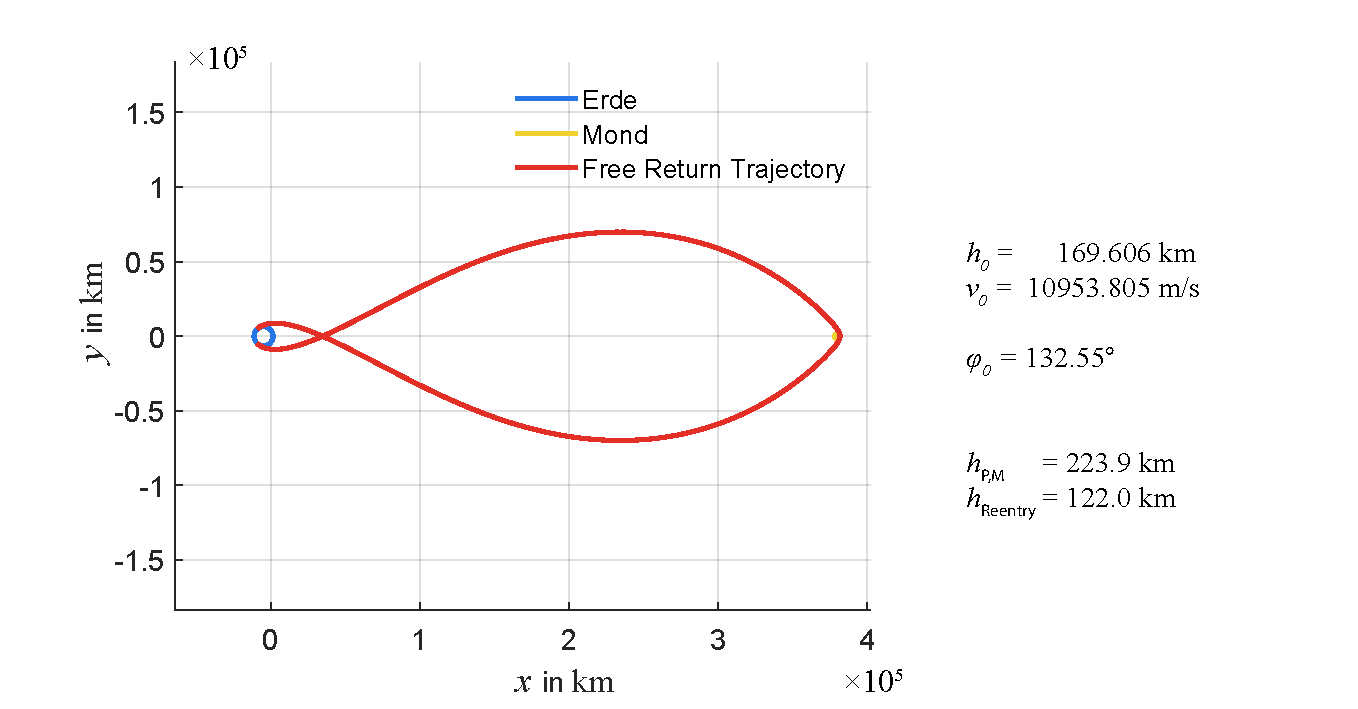
\includegraphics[width=\textwidth]{Transfer2MoonRotatingKOS.pdf} 
	\caption[Ergebnisse der numerischen Rechnung f�r das eingeschr�nkte Drei-K�rper-System Erde-Mond-Raumschiff.]{Ergebnisse der numerischen Rechnung f�r das eingeschr�nkte Drei-K�rper-System Erde-Mond-Raumschiff im mitrotierenden Koordinatensystem. Man beachte die unterschiedliche Form der Bahn, die wesentlich von der in \figref{adyn_FRT08} abweicht, was durch die unterschiedliche "`Perspektive"' des mitrotierenden Beobachters zustande kommt.}
	\label{abb:adyn_FRT10}
\end{figure}

Zum Schluss m�chten wir noch einmal bemerken, dass die FRT ein sch�nes Beispiel eines Swing-By-Man�vers (Gravity-Assist-Man�vers) (siehe \kap{adyn_gravity_assist}) beinhaltet und zwar ein Man�ver, bei welchem die Masse des Gravity-Assist-Himmelsk�rpers (in diesem Fall der Mond) abbremsend wirkt, da die Bahn nach \figref{adyn_swingby00} vor dem Himmelsk�rper liegt.

\end{subprobs}

\end{sol} 
\textcolor{blue} {$\rightarrow$ zur} \probref{adyn_rendezvous03}.\\
\noindent\rule[1ex]{\textwidth}{0.5pt}  \newpage  \clearpage

%-----------------------------------------------------------------------------------------------------------

\subsection{�bungen zu Starts aus der Erdatmosph�re und Wiedereintritt}

\noindent\rule[1ex]{\textwidth}{0.5pt} 

%-----------------------------------------------------------------------------------------------------------

\begin{sol}{prob:adyn_launch01a}\label{lsg:adyn_launch01a} %�bung25
\textbf{Bewegungsgleichungen f�r Raketenstart von Erdoberfl�che}\\

\begin{nebenrechnungNeu} {Nat�rliche Koordinaten}

(siehe \cite{Arens2008, Riley2006, Otto2019 })\\

Der zeitabh�ngige Einheitsvektor $\vec{t}$ der Tangente an die Bahnkurve (Tangentialvektor) ist definiert durch:
\begin{align}
    \vec{t} = \frac{\D \vec{r}}{\D s} ~~~\text{mit}~~~~\D s = | \D \vec{r}(t) | = \left| {\frac{\D \vec{r}}{\D t}} \right| \,  \D\,t= v(t)\; \D\,t\,,
\label{eq:adyn_NR_launch01}
\end{align}
worin $\D s$ die differentielle Bahnl�nge ist und $v$ der Betrag der Geschwindigkeit $\vec{v}$. Der Hauptnormalenvektor (ebenfalls eine Einheitsvektor) ist die 
normierte �nderung des Tangentialvektors �ber die Bahnl�nge:
\begin{align}
    \vec{n} = \frac{\D \vec{t}}{\D s} \big/ \left|\frac{\D \vec{t}}{\D s} \right|\,.
\label{eq:adyn_NR_launch02}
\end{align}
Aus $\vec{t}^2 =1 $ folgt $\D \vec{t} / \D s \cdot \vec{t} = 0$, \dh $\vec{n} \bot \vec{t}$, also $\vec{n} \cdot \vec{t} = 0$.
Damit kann man einen dritten Vektor definieren, der senkrecht auf dem Tangential- und dem Hauptnormalenvektor steht und Binormalvektor hei�t:
\begin{align}
    \vec{h} =  \vec{t} \times \vec{n}\,.
\label{eq:adyn_NR_launch03}
\end{align}
Die drei Vektoren $\vec{t},\,\vec{n},\, \vec{h}$ bilden ein (sogenanntes nat�rliches) Koordinatendreibein, das sich mit dem bewegten Objekt auf der Bahn mitbewegt und dabei sowohl einer Translation als auch Rotation unterliegt.
Die Geschwindigkeit $\vec{v}$ und die Beschleunigung $\vec{a}$ sind in diesen Koordianten dann definiert durch (\vgl Kap. 1.2.2. in Band I) 
\begin{align}
    \begin{split}
		    \vec{r} &=  v\,\vec{t}\\
        \vec{a} &=  \frac{\D}{\D t}\,\lk v\,\vec{t}\rk = \,\lek \dot{v}\,\vec{t} + v\,\dot{\vec{t}}\rek = \lek \dot{v}\,\vec{t} + v\,\vec{\omega}\times \vec{v}\rek\,.
    \end{split} \label{eq:adyn_NR_atmos03}
\end{align}
Hierin ist $\vec{\omega}$ die momentane Rotationsfrequenz des mitrotierenden \KOS definiert durch $\vec{t},\, \vec{n}$ und \vec{h}.\\

\end{nebenrechnungNeu}

Wir wollen zun�chst die momentane Rotationsfrequenz des nat�rlichen Dreibeins als Funktion von Bahnradius $r$ , Geschwindigkeit $v$ und FPA $\gamma$ berechnen. Wir betrachten dazu \figref{adyn_ueb_atmos01} und finden:
\begin{align}
    \vec{\omega} = \vec{\omega_1} + \vec{\omega_2} = (\omega_1 + \omega_2)\,\vec{h}\,,\label{eq:adyn_ueb_atmos05}
\end{align}
worin $\omega_1\,\vec{h}$ die Drehung durch die reine Bahnbewegung beschreibt und $\omega_2\,\vec{h}$ die Drehung des FPA ber�cksichtigt. Der Betrag von $\vec{\omega_1}$ ergibt sich aus \figref{adyn_ueb_atmos01} �ber $r\,\D\upsilon = |\D \vec{r}|\,\cos\gamma$ zu
\begin{align}
        \omega_1 = \dot{\upsilon} &= \frac{|\vec{v}|}{r}\,\cos\gamma = \frac{v}{r}\,\cos\gamma\, \label{eq:adyn_ueb_atmos05a} \,,
\end{align}
w�hrend der Betrag von $\vec{\omega_2}$ einfach der �nderungsrate des FPA entspricht (man beachte die Richtung!):
\begin{align}
        \omega_2 = - \dot{\gamma} \,.\label{eq:adyn_ueb_atmos05b}
\end{align}
Um die Bewegungsgleichung \eqref{eq:adyn_launch_vec},
\begin{align}
    m_\text{R}\lk t\rk \,\ddot{\vec{r}} = \vec{F}_\text{S}\lk t\rk + m_\text{R}\lk t\rk\,\vec{g}\lk \vec{r}\rk + \vec{F}_\text{D}\lk \vec{r},\dot{\vec{r}}\rk + \vec{F}_\text{A}\lk \vec{r},\dot{\vec{r}}\rk\, , \label{eq:adyn_ueb_atmos01}
\end{align}
in nat�rlichen Koordinaten schreiben zu k�nnen, schreiben wir die Kr�fte \bzw Beschleunigungen in \eqref{eq:adyn_ueb_atmos01} unter Ber�cksichtigung der Geometrie von \figref{adyn_launch02} in nat�rlichen Koordinaten (die Bewegung und alle Kr�fte sollen in einer Ebene liegen) und benutzen dabei den Angle of Attack $\alpha$ und den Flight Path Angle $\gamma$:
\begin{align}
\begin{split}
				\vec{F}_\text{S} &= F_\text{S}\,\cos\alpha\,\vec{t} + F_\text{S}\,\sin\alpha\,\vec{n}\,,~~~~\vec{F}_\text{A}  = F_\text{A}\,\vec{n}\,,~~~
        \vec{F}_\text{D} = -F_\text{D}\,\vec{t}\,,~~~\vec{g} = -g\,\sin\gamma\,\vec{t} -g\,\cos\gamma\,\vec{n}\,.
\end{split}\label{eq:adyn_ueb_atmos02}
\end{align} 
\begin{figure}[H]
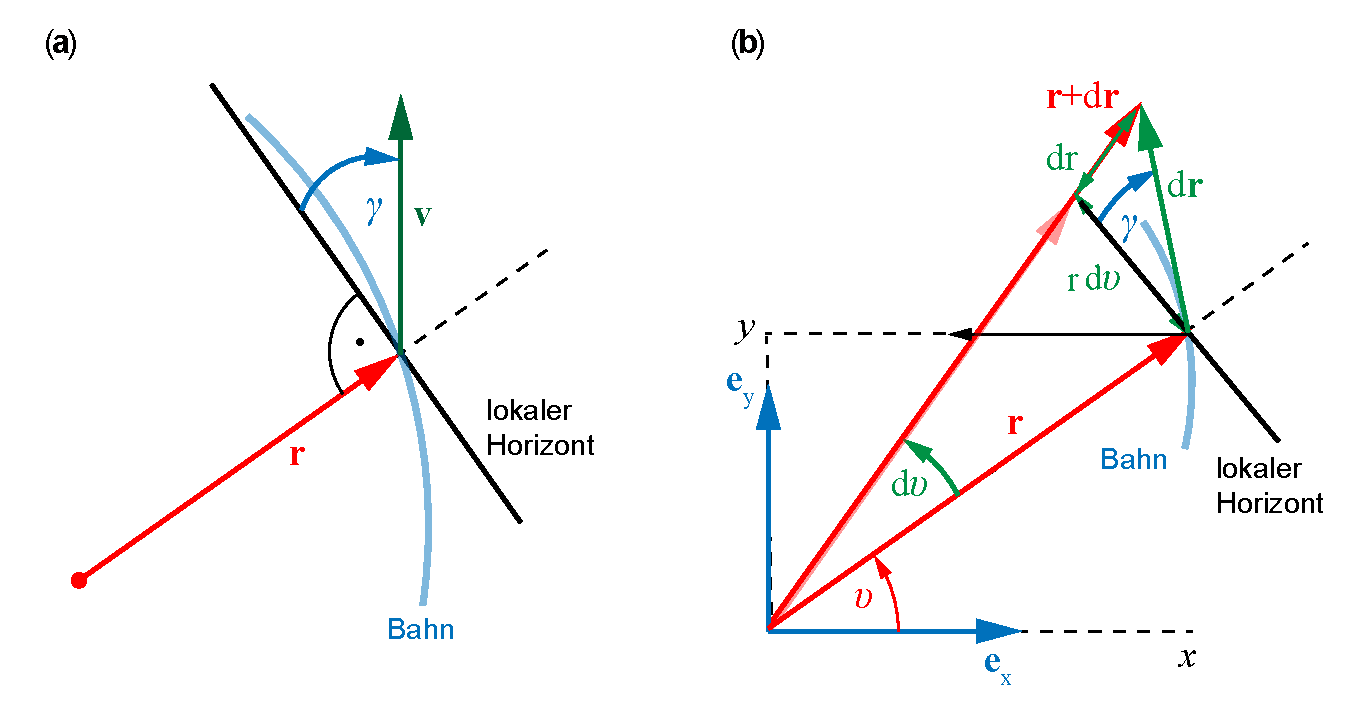
\includegraphics[width=\textwidth]{KOSReentry.pdf}
\caption[Zur Berechnung der Komponenten des Radialvektors einer Bahn im Inertialsystem der Erde.]{Zur Berechnung der Komponenten des Radialvektors einer Bahn im im Inertialsystem der Erde und im zylindrischen \KOS $\vec{t},\, \vec{n},\,\vec{h}$. \fa Lokaler Horizont, Geschwindigkeit und Flight Path Angle (FPA) $\gamma$. \fb Infinitesimale �nderungen von $r, \,\gamma$  und $v$. Der Winkel $\upsilon$ ist der Orbitalwinkel der Bahn (entspricht in etwa der wahren Anomalie) zwischen dem geozentrischen Ortsvektor zum Startpunkt und dem Ortsvektor zum Raumschiff zur Zeit $t$.}  

\label{abb:adyn_ueb_atmos01}
\end{figure}
Wir setzen \eqref{eq:adyn_ueb_atmos02} in \eqref{eq:adyn_ueb_atmos01} ein und erhalten eine Gleichung f�r $\vec{t}$ und $\vec{u}$.
\begin{align}
    \begin{split}
        \ddot{\vec{r}} &= \frac{\D}{\D t}\,\lk v\,\vec{t}\rk =  \lek \dot{v}\,\vec{t} + v\,\dot{\vec{t}}\rek = \lek \dot{v}\,\vec{t} + v \, \vec{\omega}\times \vec{v}\rek \\
        &= \lek \frac{F_\text{S}\,\cos\alpha - F_\text{D}} {m_\text{R}} \,- \,g\,\sin\gamma \rek\,\vec{t} + \lek \frac{F_\text{S}\,\sin\alpha + F_\text{A}}{m_\text{R}} - \,g\,\gamma\,\cos\gamma \rek\,\vec{n}\,.
    \end{split} \label{eq:adyn_ueb_atmos03}
\end{align}

Mit \eqref{eq:adyn_ueb_atmos05} - \eqref{eq:adyn_ueb_atmos05b} in \eqref{eq:adyn_ueb_atmos03} erhalten wir daraus jeweils eine Gleichung f�r $\vec{t}$ und 
$\vec{n}$, die jede f�r sich erf�llt sein muss, woraus folgt:
\begin{subequations}
    \begin{align}
        \dot{v}\,\vec{t} &= \lek \frac{F_\text{S}\,\cos\alpha-F_\text{D}}{m_\text{R}} - g\,\sin\gamma \rek\,\vec{t} \,, \\
        v\,\vec{\omega}\times \vec{v} &= \lk \dot{\theta}-\dot{\gamma}\rk\,\vec{h} \times v\,\vec{t}  = - \lek \frac{v^2}{r}\,\cos\gamma - v\, \dot{\gamma} \rek\,\vec{n} = \lek \frac{F_\text{S}\,\sin\alpha + F_\text{A}}{m_\text{R}} - \gamma\,g\,\cos\alpha \rek \,\vec{n}\,.
    \end{align} \label{eq:adyn_ueb_atmos04}
\end{subequations}

Nach einfacher Umformung erhalten wir schlie�lich die zwei verkoppelten skalaren Differentialgleichungen f�r $v$ und $\gamma$:
\begin{subequations}
    \begin{align}
        \dot{v} &= \frac{F_\text{S}\,\cos\alpha - F_\text{D}}{m_\text{R}} - g\,\sin\gamma\,,\\
        \dot{\gamma} &= \frac{F_\text{S}\,\sin\alpha + F_\text{A}}{v\,m_\text{R}} - \lk \frac{g}{v} -\frac{v}{r}\rk\,\cos\gamma\,~.
    \end{align}\label{eq:adyn_ueb_atmos06}
\end{subequations}

F�r den projizierten Kreisbogen $s(t)$, den das Raumschiff (eigentlich der Koordinatenursprung des mitbewegten \KOS) auf der Erdoberfl�che s(t) beschreibt, den Abstand des Raumschiffs vom Erdmittelpunkt  $r$ \bzw seine H�he $h$ �ber der Erdoberfl�che finden wir leicht aus geometrischen �berlegungen (\figref{adyn_launch02} und \figref{adyn_ueb_atmos01}):

\begin{subequations}
    \begin{align}
        \dot{h} &= v\,\sin\gamma\,,\\ 
        \dot{s} &= \frac{R_\text{E}}{r}\,v\,\cos\gamma \,=\, \frac{1}{1+h/R_\text{E}}\,v\,\cos\gamma  \,.
    \end{align}\label{eq:adyn_ueb_atmos07}
\end{subequations}

Das Differential-Gleichungssystem \eqref{eq:adyn_ueb_atmos06} und \eqref{eq:adyn_ueb_atmos07} bestimmt damit vollst�ndig die Aufstiegsbahn im mitbewegten KOS. Diese Bahn liegt in der durch die Richtungen von $s$ und $h = r - R_\text{E}$ bestimmten Ebene. 

\end{sol} 
\textcolor{blue} {$\rightarrow$ zur} \probref{adyn_launch01a}.\\
\noindent\rule[1ex]{\textwidth}{0.5pt}  \newpage  \clearpage
%-----------------------------------------------------------------------------------------------------------

\begin{sol}{prob:adyn_launch01}\label{lsg:adyn_launch01} %�bung26
\textbf{Raketenstart von verschiedenen Weltraumzentren}\\

\begin{subprobs}
\subprob{Allgemeine Betrachtungen}

\begin{figure}[H]
	\includegraphics[width=\textwidth]{Aufstiegsbahnen.pdf} 
	\caption[Transfer eines Raumschiffs von der Erdoberfl�che in einen Erdorbit �ber eine Hohmann-Ellipse.]{Transfer eines Raumschiffs von der Erdoberfl�che in einen Erdorbit �ber eine Hohmann-Ellipse. \fa idealisierter Fall ohne Reibung \fb realistischer Fall bei Vorhandensein einer Atmosph�re. Im idealisierten Fall w�rde man die Rakete horizontal direkt in die Hohmann-Ellipse starten lassen, im Fall \fb aus aerodynamischen und strukturellen senkrecht zum Horizont und f�hrt dann eine Nickkorrektur aus, um das Raumschiff einen \textit{Gravitation Turn}\index{Gravitation Turn}\index{Schwerkraftdrehung}  machen zu lassen. Siehe unten im Text.}
	\label{abb:adyn_launch_lsg_Schema}
\end{figure}

Wir k�nnen die Berechnungen vorteilhafter weise im in \kap{adyn_launch} eingef�hrten mitbewegten \KOS tun, da es uns nur um die Dynamik und nicht um eine geographische Berechnung der Bahn geht.\\
Zielstellung der Berechnung ist, das Raumschiff in eine Kreisbahn mit der H�he $h_\text{K}$ (numerische Werte beispielhaft f�r $h_\text{K}= \SI{300}{\km}$) zu bringen.\\
Ohne Atmosph�re w�rde man das Raumschiff horizontal in Richtung Osten von der Erde starten lassen (\figref{adyn_launch_lsg_Schema}a  und zwar mit einem Geschwindigkeitsbudget von
\begin{align}
	\Delta v_0 = \sqrt{\frac{G\,M_\text{E}}{R_\text{E}+h}} - \Delta v_\text{E,t} = \sqrt{\frac{G\,M_\text{E}}{R_\text{E}+h}} - \frac{2\pi\,R_\text{E}\,\cos\varphi_0}{\SI{86125}{\second}}\approx \SI{7.7309}{\km\per\second} - \SI{0.465}{\km\per\second}\,\cos\varphi_0 \,,
\end{align}
worin $\varphi_0$ die geographische Breite des Abschussortes ist und $\Delta v_\text{E,t}$ die Tangentialgeschwindigkeit auf der Erdoberfl�che der Erdrotation bezeichnet.
Das Raumschiff bewegt sich in diesem idealisierten Fall auf einer Hohmann-Ellipse (\kap{adyn_hohmann_transfer}) mit der Halbachse $a_\text{T}$ und der Exzentrizit�t $e_\text{T}$ (Numerische Werte f�r $h=\SI{300}{\km}$.)
\begin{align*}
	a_\text{T} &= \frac{1}{2} \, \lk R_\text{E} + h + R_\text{E} \rk = R_\text{E}+\frac{h}{2} \approx \SI{6528}{\km} \,,\\
  e_\text{T} &= \frac{h}{2R_\text{E}+h } \approx 0.022978\,.
\end{align*}
und br�uchte 
\begin{align}
	t_\text{f} = t_\text{T}= \pi\sqrt{\frac{a_\text{T}{}^3}{G\,M_\text{E}}} \approx \SI{43.5}{\minute}\,,
\end{align}
um in die Umlaufbahn zu gelangen, wo noch einmal entsprechend Gleichung \eqref{eq:adyn_hohmann04} ein Burn notwendig ist, um das Raumschiff aus der elliptischen Bahn in die Kreisbahn zu bringen.\\
In einem realistischen Fall (\figref{adyn_launch_lsg_Schema}b, \dh unter Ber�cksichtigung von Drag, wird das Raumschiff nach der Schubphase zum Zeitpunkt $t_\text{T}$ an einem �bergangspunkt T auf die Hohmann-Ellipse treffen. Dort m�ssen dann folgende Bedingungen erf�llt sein:\footnote{Hierbei haben wir die Gleichungen \eqref{eq:adyn_reentry02} benutzt. Wir hatten ja in \kap{adyn_reentry} darauf hingewiesen, dass diese Gleichungen sowohl f�r den De-Orbit als auch die Startphase gelten.}
\begin{subequations}
\begin{align}
    \cos\gamma_\text{T} &= \cos\gamma(t_\text{T})=\frac{1+e_\text{T}\,\cos\upsilon_\text{T}}{\sqrt{1+2e_\text{T}\,\cos\upsilon_\text{T} +e_\text{T}{}^2}}\,,\label{eq:adyn_launch_lsg01a}\\
    v_\text{T} &= v(t_\text{T}) = \sqrt{\frac{G\,M_\text{E}}{a_\text{T}(1-e_\text{T}{}^2}}\,\sqrt{1+2e_\text{T}\,\cos\upsilon_\text{T}+e_\text{T}{}^2} \label{eq:adyn_launch_lsg01b} \,,\\
    h_\text{T} &= r(t_\text{T}) - R_\text{E} = \frac{a_\text{T}\,\lk 1-e_\text{T}{}^2\rk}{1+e_\text{T}\,\cos\upsilon_\text{T}} - R_\text{E}\,.\label{eq:adyn_launch_lsg01c}
\end{align} \label{eq:adyn_launch_lsg01}
\end{subequations}

Hierin ist $\gamma_\text{T}$ der FPA und $\upsilon_\text{T}$ die wahre Anomalie der Hohmann-Ellipse zum Zeitpunkt $t_\text{T}$.\\
F�r den Startzeitpunkt $t=0$ gilt:
\begin{subequations}
\begin{align}
    \gamma_0 &= \gamma(t = 0)=  \pi/2 \label{eq:adyn_launch_lsg02a}\,,\\
    v_0 &= v(t=0) = 0 \label{eq:adyn_launch_lsg02b} \,,\\
    h_0 &= h(t=0) = 0 \,.\label{eq:adyn_launch_lsg02c}
\end{align} \label{eq:adyn_launch_lsg02}
\end{subequations}

Die Schubphase muss also durch geeignete Steuerung des Anstellwinkles (AoA) $\alpha(t)$, der Massenverlustrate $\dot(m)(t)$, des Schubs $F_\text{S}(t)$ und der Wahl von $\upsilon(t)$ so gestaltet werden, dass als Ergebnis der zeitlichen Entwicklung des DGL-Systems \eqref{eq:adyn_launch01} die Bedingungen \eqref{eq:adyn_launch_lsg01} erf�llt werden und dies bei m�glichst geringem Treibstoffverbrauch \bzw gro�er Nutzlast. Wir wissen nun aus \kap{adyn_launch}, Gleichung \eqref{eq:adyn_launch07}, dass ein AoA verschieden von Null zu Verlusten zus�tzlich zu den unvermeidlichen Gravitations- und Reibungsverlusten f�hrt. Andererseits zeigt die formale Integration von \eqref{eq:adyn_launch01} auch, dass ein $\alpha$ verschieden von Null zu einer gew�nschten Ver�nderung des FPA f�hrt.
\begin{subequations}
\begin{align}
    v(t_\text{T}) &= \int\limits_0^{t_\text{T}} \frac{F_\text{S}}{m_\text{R}}\,\D t' - \underbrace{\int\limits_0^{t_\text{T}} \frac{F_\text{D}}{m_\text{R}}  \,\D t'}_{\mathrm{Reibungsverlust}} - \underbrace{\int\limits_0^{t_\text{T}} \frac{F_\text{S}\,(1-\cos\alpha)}{m_\text{R}}  \,\D t'}_{\mathrm{Steuerungsverlust}}  - \underbrace{\int\limits_0^{t_\text{T}} g\,\sin\gamma \,\D t'}_{\mathrm{Gravitationsverlust}} \label{eq:adyn_launch_lsg03a} \,, \\
    \gamma(t_\text{T}) &= \frac{\pi}{2}+ \underbrace{\int\limits_0^{t_\text{T}} \frac{F_\text{S}\,\sin\alpha}{m_\text{R}\,v}  \,\D t'}_{\mathrm{Steuerungsverlust}} -  - \underbrace{\int\limits_0^{t_\text{T}}\frac{g}{v}\,\cos\gamma \,\D t'}_{\mathrm{Gravitationsverlust}} + \underbrace{\int\limits_0^{t_\text{T}}\frac{v}{r}\,\cos\gamma \,\D t'}_{\mathrm{Zentrifugalgewinn}} \nonumber \\
		&= \frac{\pi}{2} + \underbrace{\int\limits_0^{t_\text{T}} \frac{F_\text{S}\,\sin\alpha}{m_\text{R}\,v}  \,\D t'}_{\mathrm{Steuerungsverlust}} - \underbrace{\int\limits_0^{t_\text{T}} \lk \frac{g}{v} - \frac{v}{r} \rk \,\cos\gamma  \,\D t'}_{\mathrm{Gravitation~Turn}} \,. \label{eq:adyn_launch_lsg03b}
\end{align} \label{eq:adyn_launch_lsg03}
\end{subequations}

Das erscheint zun�chst wie ein Dilemma, denn erreicht man eine gro�e �nderung von $\gamma$, verliert man an Geschwindigkeit $v$. Zum Gl�ck gibt es, wie man am 2. Term in \eqref{eq:adyn_launch_lsg03b} sieht, den \textit{Gravitation Turn} (in etwa Schwerkraftdrehung), der sich aus der Kombination von Schwerkraft und Zentrifugalkraft\footnote{Da wir die Gleichungen \eqref{eq:adyn_launch01} im mitbewegten \KOS geschrieben haben tritt in diesen die Zentrifugalkraft auf.} f�r $\gamma \neq \pi/2$ ergibt und der automatisch Null wird, wenn $v$ gegen die Kreisbahngeschwindigkeit $\sqrt{g\,r}$ geht. Der Vorteil der Schwerkraftdrehung besteht darin, dass der Schub nicht dazu verwendet werden muss, um die Richtung des Raumfahrzeugs zu �ndern, und noch wichtiger, dass w�hrend der anf�nglichen Aufstiegsphase die Rakete eine Anstellwinkle von Null behalten kann, welcher die aerodynamischen Belastungen der Rakete erheblich reduziert.\\
Wie findet nun ein Raketenstart unter Nutzung der Schwerkraftdrehung statt?  Nach dem vertikalen Start gewinnt die Rakete zun�chst an Vertikalgeschwindigkeit und H�he. W�hrend dieses Teils des Starts wirkt der Schwerkraftwiderstand, der in der n�chsten Phase des Starts mit dem sogenannten Pitchover-Man�ver (Nick-Korrektur) reduziert wird.\footnote{Die Nick-Korrektur wird bei immer noch relativ geringen Vertikalgeschwindigkeiten durchgef�hrt, um aerodynamische Belastungen auf das Raumschiff zu vermeiden. Der Neigungswinkel des Pitchover-Man�ver betr�gt nur wenige Grad, es gibt aber auch F�lle, bei denn relativ gro�e Winkel (einige zehn Grad) verwendet werden. Die Nickkorrektur dauert \ia nur sehr kurz und ist der einzige Moment w�hrend der Aufstiegsphase, in dem der Schub zum Lenken genutzt wird. Nach dem Pitchover-Man�ver bleibt der AoA f�r den Rest des Aufstiegs bei Null, so dass auch der Auftrieb vernachl�ssigt werden kann.}
Das Pitchover-Man�ver dient zwei Zwecken. Erstens dreht es die Rakete leicht, so dass ihre Flugbahn nicht mehr vertikal verl�uft, und zweitens bringt es die Rakete auf den richtigen Kurs (Startazimut)\index{Startazimut} f�r ihren Aufstieg in die Umlaufbahn. Siehe dazu auch den folgenden L�sungsteil zum Startfenster (Launch Window) und  Startrichtung (Startazimut)). 

\subprob{Startphase einer dreistufigen Rakete (Ariane-1) im $\vec{t},\, \vec{n}$ und \vec{h} - \KOS.}

Im \mscr~\mladynref{Raketenstart2Orbit01.m} und \mladynref{Raketenstart2Orbit02.m} berechnen wir die f�r eine dreistufige Rakete den Transfer in den erdnahem Orbit.

\begin{figure}[H]
	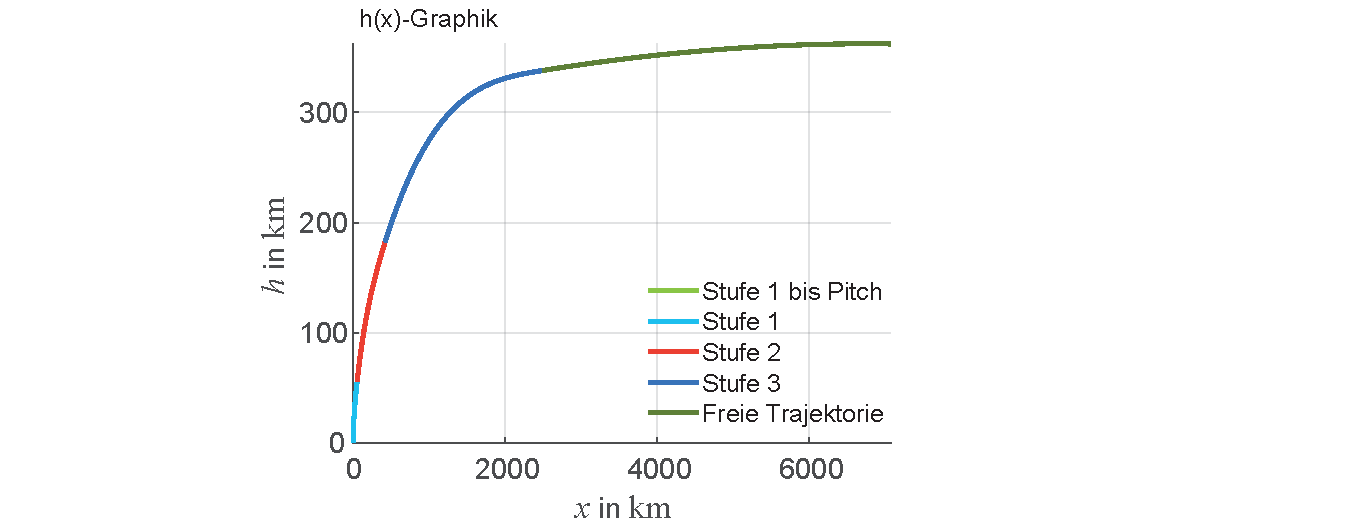
\includegraphics[width=\textwidth]{Startkurve.pdf} 
	\caption[Trajektorie nach Start von der Erdoberfl�che.]{Trajektorie nach Start von der Erdoberfl�che. Parameter siehe \mladynref{Raketenstart2Orbit02.m}.}
	\label{abb:adyn_launch_lsg02}
\end{figure}

\begin{figure}[H]
	\includegraphics[width=\textwidth]{Raketenstart2OrbitUebersicht.pdf} 
	\caption[Geschwindigkeit, Bahnh�he, FPA und Masse nach Start von der Erdoberfl�che. ]{Geschwindigkeit, Bahnh�he, FPA und Masse nach Start von der Erdoberfl�che f�r eine dreistufige Rakete bis zum �bergangspunkt (hier mit $h_\text{T} = \ca \SI{350}{\km}$ angenommen. Parameter siehe \mladynref{Raketenstart2Orbit02.m}.}
	\label{abb:adyn_launch_lsg03}
\end{figure}

\subprob{Startfenster (Launch Window) und  Startrichtung (Startazimut)}

Bisher haben wir uns nur mit der Dynamik und den energetischen Fragen eines Starts von der Erdoberfl�che und des anschlie�enden Transfer in eine gew�nschte Umlaufbahn besch�ftigt, nicht aber mit den Fragen nach der Zeit und den r�umlichen-geometrischen Bedingungen. Man k�nnte nat�rlich prinzipiell das Raumschiff zu jedem beliebigen Zeitpunkt starten und es auch an einen beliebigen Ort schie�en, um dann mit verschiedenen Bahnman�ver die Zielbahn zu erreichen. Aber das w�re eine enorme Verschwendung von Treibstoff. 

Unter einem Startfenster verstehen wir den Zeitraum, in welchem ein Raumschiff direkt in den gew�nschten Orbit \bzw auf eine geeignete Transferbahn (siehe vorhergehenden Abschnitt) gestartet werden kann. Dazu m�ssen wir abh�ngig vom gew�nschten Orbit und der geographischen Position des Abschussortes eine geeignet Startzeit und einen geeigneten Startwinkel finden. 

Hierbei gilt es zwei F�lle zu unterscheiden, zum einen, wenn die Inklination der gew�nschten Bahn $i$ gr��er oder gleich der geographischen Breite $\varphi_0$ des Startplatzes ist und zum anderen, wenn die Bahnneigung kleiner als die geographischen Breite ist. Wir werden sehen, dass es im zweiten Fall M�glichkeit gibt, direkt in den Orbit zu starten. 

Ein geeigneter Startzeitpunkt ist gegeben, wenn sich der Startort in der Position der Sternzeit des Startfensters (LWST) befinden, wobei  �in Position� hei�t, dass sich  Startplatz (bzw genauer der Breitenkreis des Startorts) und die gew�nschte Bahnebene schneiden. Wir betrachten dazu das sph�rische Dreieck in \figref{adyn_launch_lsg02}, welches durch drei Linien/Seiten gegeben ist. Die erste Seite ergibt sich aus der Bodenspur f�r die Umlaufbahn, die zweite aus der �quatorlinie und die dritte aus dem L�ngenkreis des Startplatzes. 
Aus \figref{adyn_launch_lsg02} entnehmen wir ferner noch weitere Gr��en mit folgenden Definitionen und Beziehungen:\\

\begin{tabular}[h]{ll}
LWST &~Sternzeit des Startfenster\index{Startfenster} (Launch Window Siderial Time)\index{Launch Window Siderial Time}\\
$\delta$ &~Hilfswinkel in Startrichtung\\
$\theta$ &~Standortwinkel des Startfensters\\
$\beta$  &~Startazimut\index{Startazimut}\\
$\Omega$ &~Rektaszension des aufsteigenden Knotens\\
\end{tabular}

\begin{figure}[H]
	\includegraphics[width=\textwidth]{BestimmungLWST.pdf} 
	\caption[LST und sph�risches Dreieck zur Bestimmung des LWST.]{LST \fa und sph�risches Dreieck zur Bestimmung des LWST \fb.}
	\label{abb:adyn_launch_lsg04}
\end{figure}

Mit dem Winkelkosinussatz der sph�rischen Trigonometrie \cite{Meyers1995} $~\cos \alpha = -\cos\beta\,\cos\gamma\,+\,\sin\beta\,\sin\gamma\,\cos a$ 
finden wir 
\begin{align*}
\cos i = -\cos(\pi/2)\,\cos\delta\,+\,\sin(\pi/2)\,\sin\delta\,\cos \varphi_0\,,
\end{align*}
was sich mit $\cos(\pi/2) = 0$ und $\sin(\pi/2) = 1$ zu
\begin{align}
\sin \delta = \cos i / \cos \varphi_0\, \label{eq:adyn_launch_lsg04}
\end{align}
vereinfacht. F�r das rechtwinklige sph�rische Dreieck gilt au�erdem \cite{Meyers1995}: $\cos \delta = \cos \theta \,\sin i~$, 
woraus schlie�lich mit \eqref{eq:adyn_launch_lsg03}
\begin{align}
\cos \theta = \frac{\cos \delta }{\sin i} = \frac{\sqrt{1 - \sin^2\delta}}{\sin i} = \frac{\sqrt{\lk 1 - \cos^2 i / \cos^2 \varphi_0 \rk}}{\sin i}
\label{eq:adyn_launch_lsg05}
\end{align}
folgt. F�r die n�rdliche Hemisph�re ergibt sich damit das LWST zu:
\begin{align}
\text{In der N�he des aufsteigenden Knotens: ~~~}\mathrm{LWST}_\text{auf} &= \Omega + \theta ~\,, \label{eq:adyn_launch_lsg06} \\
\text{In der N�he des absteigenden Knotens: ~~~~}\mathrm{LWST}_\text{abs} &= \Omega + (180\degree - \theta) \,. \label{eq:adyn_launch_lsg07}
\end{align}

\begin{figure}[H]
	\includegraphics[width=\textwidth]{StartAzimute.pdf} 
	\caption[Startazimut.]{Startazimut in der N�he des \fa aufsteigenden Knotens und des \fb absteigenden Knotens.}
	\label{abb:adyn_launch_lsg05}
\end{figure}

Es gibt noch einen letzten Winkel, der ber�cksichtigt werden muss, n�mlich das Startazimut $\beta$, \dh die Richtung in die gestartet werden soll. Dies ist der Winkel zwischen dieser �Aufw�rts�-Richtung und der Startrichtung (\figref{adyn_launch_lsg03}) und wird von der Nordrichtung aus im Uhrzeigersinn gemessen. Er ist vom Betrag her gleich dem Winkel $\delta$, womit wir schreiben k�nnen:
\begin{align}
\beta = \arcsin \frac{\cos i}{\cos \varphi_0}\,. \label{eq:adyn_launch_lsg08}
\end{align}
Wir erkennen an dieser Beziehung auch, dass die erreichbare Neigung der Bahn immer gr��er als die geographische Breite des Startortes sein muss, andernfalls w�rde $\beta$ komplexe Werte annehmen. Es gilt also immer $i \geq \varphi_0$, wobei die minimal Bahnneigung bei einem Startazimut von $90\degree$ (entspricht Ost) erreicht wird (\figref{adyn_launch_lsg04}).\\
F�r ein gegebenes $\Omega$ der Bahn gibt es  zwei L�sungen oder Startzeiten pro Rotation. Bei jeder davon kann man dann zwischen prograden und retrograden Umlaufbahnen w�hlen. Diese werden entlang der berechneten Startazimute in Richtung Norden oder S�den verlaufen, wobei die Startfenster einige Zeit auseinander liegen. Es gibt nur eine L�sung, wenn die Neigung genau dem Breitengrad entspricht.  Wir wolle zwei Beispiele angeben (siehe auch \mscr~\mladynref{Raketenstart2Orbit03.m}).

\begin{figure}[H]
	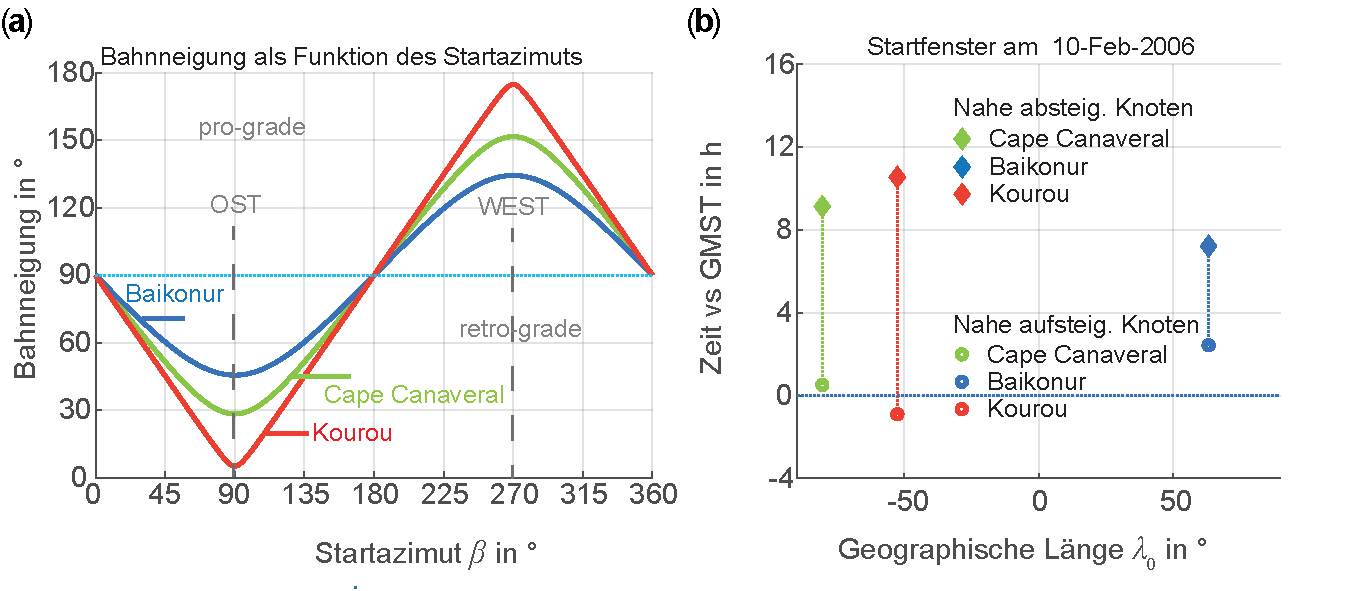
\includegraphics[width=\textwidth]{StartAzimuteStartFenster.pdf} 
	\caption[Bahnneigung und Startfenster als Funktion des Startazimuts und Startfenster zur ISS.]{Bahnneigung \fa und Startfenster \fb als Funktion des Startazimuts f�r verschiedene Weltraumzentren.}
	\label{abb:adyn_launch_lsg06}
\end{figure}

Die Internationale Raumstation umkreist die Erde mit einer Neigung von $51.6\degree$. F�r einen Start von Cape Canaveral (Breitengrad $28.383\degree$) \bzw vom Kosmodrom Baikonur (Breitengrad 45.617�) in die ISS-Umlaufbahn berechnen sich die Startazimute zu:
ergibt sich dann:
\begin{align*}
\beta_\text{CC}  &= \arcsin \frac{\cos(51.6\degree)}{\cos(28.383\degree)} = 44.98\degree~~ \text{\bzw}~~135.02\degree\,,\\ 
\beta_\text{Bai} &= \arcsin \frac{\cos(51.6\degree)}{\cos(45.617\degree)} = 63.21\degree~~ \text{\bzw}~~116.80\degree\,. 
\end{align*}

Die Berechnung der  Startfenster und Startazimute f�r die ISS f�r den 10. M�rz 2006 ist im \mscr~\mladynref{Raketenstart2Orbit03.m}\, ausgef�hrt.
F�r die ISS haben wir daf�r folgende Bahnparameter f�r Anfang 2006 benutzt \cite{JPL2020}.\\

\begin{tabular}{L{7cm}C{2cm}L{4cm}}
Epoche & $t_\text{epoch}$ & 09.02.2006 20:26:00.0000\\
Inklination &$i$ & $51.6448\degree$\\
Rektaszension des aufsteigenden Knotens & $\Omega$ & $122.3522\degree$\\
numerische Exzentrizit�t der Umlaufbahn & $e$ & 0.0008835\\
Argument des Perig�ums & $\omega$ &$257.3473\degree$\\
Mittlere Anomalie & $M$ & $251.7436\degree$\\
Mittlere Bewegung & $n$ & $ \SI{15.74622749}{\per\day}$\\
\end{tabular}
\medskip

Die Sternzeit in Greenwich bestimmt man aus dem Julianischen Datum JD f�r den Zeitpunkt 0:00 h UTC. Zun�chst berechnet man das Julianische Datum in Jahrhunderten seit dem 1.1.2000. 
	\[ T\,=\,\frac {JD-2451545.0}{36525} \]
und daraus die mittlere Sternzeit f�r Greenwich f�r den Zeitpunkt 0:00 h UTC:
\begin{align}
\mathrm {GMST_0} \,&=\,6^{\mathrm {h} }41^{\mathrm {m} }50.54841^{\mathrm {s}}\,+\,8640184.812866^{\mathrm {s} }\, T\,+\,0.093104^{\mathrm {s} }\, T^{2}\,-\,0.0000062^{\mathrm {s} }\, T^{3}\\
&=\,24110.54841^{\mathrm {s} }+8640184.812866^{\mathrm {s} }\, T \, + \,0.093104^{\mathrm {s} }\, T^{2}\,-\,0.0000062^{\mathrm {s} }\, T^{3}\\
&=\,100.46061837\degree+36000.770053608\degree\, T\,+\,0.000387933\degree\, T^{2}\,-\,(T^{3}/38710000)\degree
\end{align}
F�r einen Beobachter auf der geographischen L�nge $\lambda_0$ muss man die Sternzeit noch auf seine Ortssternzeit LST umrechnen:
\begin{align}
\mathrm {LST} \,&\,=\mathrm {GMST} +\lambda~~~{\text{f�r GMST im Gradma�}}
\end{align}

Wir verweisen auf das \mscr~\mladynref{Raketenstart2Orbit03.m} und auch auf \kap{hm_zeitdefinition}.


\subprob{Berechnung der 3D-Trajektorien im Inertialsystem}


F�r die weiteren Berechnungen muss man ber�cksichtigen, das wir alle Gr��en wie \zb das in \eqref{eq:adyn_launch_lsg08} abgeleitete Startazimut im Inertialsystem berechnet hatten. Da wir jedoch die Rakete von der rotierenden Erdoberfl�che starten, muss man die Erddrehung entsprechend ber�cksichtigen, was zu einer leichten Korrektur des Startazimuts und auch des Geschwindigkeitsbudgets f�hrt. Wir wollen ab sofort zur besseren Unterscheidung die Gr��en im mitbewegten System gestrichen kennzeichnen, die im Inertialsystem als ungestrichen.
So ist \zb f�r eine Umlaufbahn von 300 km H�he das Mindestgeschwindigkeitsbudget $\Delta \vec{v}$ (ohne Reibung und Reserven) durch $\Delta \vec{v} = \Delta v\,(\sin \beta\,\veceX + \cos \beta\,\veceY)$ mit $\Delta v = \SI{7.7309}{\km\per\second}$ gegeben, wobei die Einheitsvektoren in der Bahnebene liegen und in die Ost- \bzw Nordrichtung zeigen. Am einfachsten macht man sich nun an Hand von \figref{adyn_launch_lsg07} klar, dass zur Berechnung des Geschwindigkeitsbudget $\Delta \vec{v}'$ im Nichtinertialsystem die vektorielle Differenz von $\Delta \vec{v}$ und $\Delta v_\text{E,t}\,\veceX = \SI{0.465}{\km\per\second}\,\cos\phi_0$ (\vgl \eqref{eq:adyn_launch10}) gebildet werden muss. Man erh�lt:
\begin{align}
\Delta v' = \Delta v \, \sqrt{\lk \sin \beta \, - \Delta v_\text{E,t}/ \Delta v \rk^2 + \cos^2 \beta}\,. \label{eq:adyn_launch_lsg09}
\end{align}
Das Startazimut im mitbewegten System $\beta'$ ergibt sich dann zu:
\begin{align}
\beta' = \arctan \lk \frac{\Delta v\,\sin \beta\, - v_\text{E,t}}{\Delta v\,\cos \beta\,} \rk\,. \label{eq:adyn_launch_lsg10}
\end{align}
F�r einen Start zur ISSS von Cape Canaveral �ndert es sich beispielsweise von $44.98\degree$ auf $42.76\degree$. Auch der FPA rechnet sich enstprechend um zu:
\begin{align}
\gamma = \arcsin \lk \frac{\Delta v'}{\Delta v}\,\sin \gamma' \rk\,. \label{eq:adyn_launch_lsg11}
\end{align}

\begin{figure}[H]
	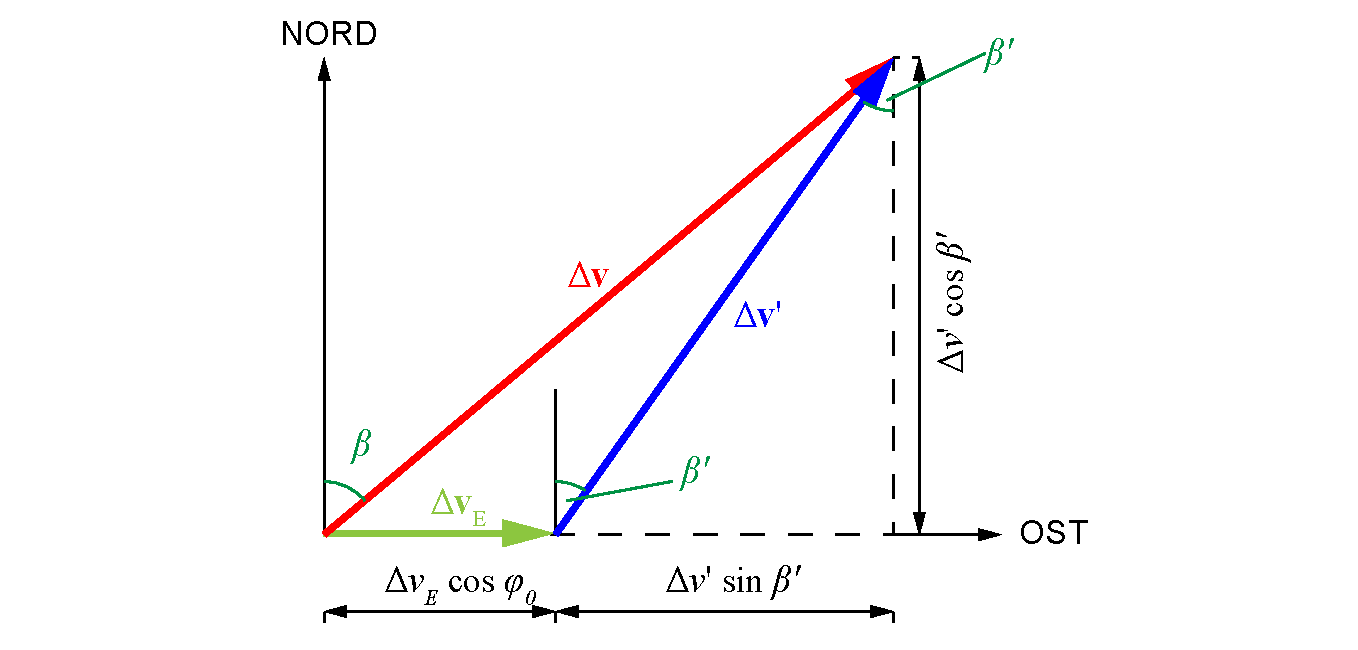
\includegraphics[width=\textwidth]{StartAzimutInertial.pdf} 
	\caption[Ber�cksichtigung der Erdrotation beim Start von Raketen.]{Ber�cksichtigung der Erdrotation beim Start von Raketen.}
	\label{abb:adyn_launch_lsg07}
\end{figure}

F�r die Berechnung der 3D-Trajektorien haben wir drei M�glichkeiten:
\begin{enumerate}[a)]
	\item Wir betrachten alles im geozentrisch-raumfesten Inertialsystem und l�sen numerisch die Bewegungsgleichung \eqref{eq:adyn_launch_vec} in 3 Dimensionen. Dabei m�ssen wir bei den Anfangsbedingungen die von der Rakete mitgenommene Rotation der Erde nach \eqref{eq:adyn_launch_lsg09} ber�cksichtigen, ebenso wie das umgerechnete Startazimut $\beta$ und den Anfangs-FPA $\gamma_0$ nach \eqref{eq:adyn_launch_lsg10} \bzw \eqref{eq:adyn_launch_lsg11}. Man beachte, dass die beiden Gr��en im topozentrischen System definiert sind und mit den Ortskoordinaten des Startorts in das Inertialsystem umgerechnet werden m�ssen.\\
	Bei der Berechnung der Reibung muss man ber�cksichtigen, dass die Atmosph�re mitrotiert und folglich die f�r die Reibung ma�gebliche aktuelle Geschwindigkeit $v'$ aus der im Inertialsystem geltenden Geschwindigkeit in $v$ umgerechnet werden muss:
\begin{align}
\begin{split}
		\vec{v}'(t) &= \vec{v}(t) - \vec{v}_\text{E,0} ~~~\text{mit}~~~\vec{v}_\text{E,0} = \vec\omega_\text{E} \times \vec{r}_0 \,.
\end{split} \label{eq:adyn_launch_lsg12}
\end{align}
Die Bewegungsgleichung lautet also:
\begin{align}
\begin{split}
		\vec{\ddot{r}}\begin{pmatrix} \ddot{x}\\ \ddot{y} \\ \ddot{z} \end{pmatrix} &=  \frac{\vec{F}_\text{S}(t) + \vec{F}_\text{G}(t) - \vec{F}_\text{D}(t)}{m_\text{R}(t)} = 
		\frac{F_\text{S}(t)}{m_\text{R}(t)\,v(t)} \begin{pmatrix} \dot{x}\\ \dot{y} \\ \dot{z} \end{pmatrix} 
 - \frac{G\,M_\text{E}}{\left| \vec{r}(t) \right|^3} \begin{pmatrix} x \\y\\z \end{pmatrix}
 - \frac{\varrho(r)\, v'\, A \,c_\text{D}}{m_\text{R}(t)} \begin{pmatrix} \dot{x}'\\ \dot{y}'\\ \dot{z}' \end{pmatrix}\,.
\end{split} \label{eq:adyn_launch_lsg13}
\end{align}
Die Nickkorrektur wird wie folgt berechnet:\\ 
Nach Bestimmung der Geschwindigkeit zum Zeitpunkt kurz vor der Nickkorrektur $\vec{v}(t=t_\text{Nick-})$, die sich ohne der mitgenommenen
Rotation der Erde ergibt (also nur die Geschwindigkeitszunahme durch den Schub), erfolgt 
die Drehung des Geschwindigkeitsvektors/Schubvektors um den Nickwinkel $\gamma_\text{N}$ in Richtung des Startazimuts. Diese Drehung wird im Horizontsystem 
mit folgender Drehmatrix $\mathbb{R}_\text{Nkorr}$ beschrieben, wobei hierbei zuerst die
Nickkorrektur und dann die Ausrichtung auf das Azimut ausgef�hrt wird. Die dazu notwendigen Berechnung der Drehmatritzen f�hren wir in einer Nebenrechnung aus:

\begin{nebenrechnungNeu} {Einheitsvektoren und Transformationsmatrix}

\begin{align*}
    \vec{r} &= r\,\begin{pmatrix} \sin\theta\,\cos\phi \\ \sin\theta\,\sin\phi \\ \cos\phi \end{pmatrix} ~~ \text{\bzw in geograph. Koord.}~~~ \vec{r} = r\,\begin{pmatrix} \cos\varphi\,\cos\lambda \\ \cos\varphi\,\sin\lambda \\ \sin\varphi \end{pmatrix}\\
    \vec{e}_\text{r} &= \frac{\d\vec{r}}{\d r} \;= \;\begin{pmatrix} \sin\theta \,\cos\phi \\ \sin\theta\,\sin\phi \\ \sin\phi \end{pmatrix}\; \widehat{=} \;\begin{pmatrix} \cos\varphi\,\cos\lambda \\ \cos\varphi\,\sin\lambda \\ \sin\varphi \end{pmatrix}\\
     \vec{e}_\theta &= \frac{1}{r}\,\frac{\d\vec{r}}{\d \theta}\;=\; \begin{pmatrix} \cos\theta \,\cos\phi \\ \cos\theta \,\sin\phi \\ -\sin\phi \end{pmatrix}\;\widehat{=}\;\vec{e}_\varphi = \frac{1}{r}\,\frac{\d\vec{r}}{\d \varphi}\;=\; \begin{pmatrix} -\sin\varphi \,\cos\lambda \\ -\sin\varphi\,\sin\lambda \\ \cos\varphi \end{pmatrix} \\
     \vec{e}_\phi &= \frac{1}{r\,\sin\theta}\,\frac{\d\vec{r}}{\d \phi}\;=\; \begin{pmatrix} -\sin\phi\\ \cos\phi \\ 0 \end{pmatrix}\;\widehat{=}\;\vec{e}_\lambda = \frac{1}{r\,\cos\varphi}\,\frac{\d\vec{r}}{\d \lambda}\;=\; \begin{pmatrix} -\sin\lambda \\ \cos\lambda\\ 0 \end{pmatrix} \\
    \rightarrow \mathbb{S} &= \lk \vec{e}_\text{r},\,\vec{e}_\theta,\,\vec{e}_\phi \rk \;=\; \begin{pmatrix} \cos\varphi\,\cos\lambda & -\sin\phi\,\cos\varphi & -\sin\lambda \\ \cos\varphi\,\sin\lambda & -\sin\varphi\,\cos\lambda & \cos\lambda \\ \sin\varphi & \cos\varphi& 0 \end{pmatrix}
\end{align*}

\end{nebenrechnungNeu}

Wir erhalten damit:

\begin{align}
\begin{split}
		\mathbb{R}_\text{Nkorr} &= \mathbb{R}_\text{A}\, \mathbb{R}_\text{N} ~~\text{mit}~~\\
		\mathbb{R}_\text{N} &= \begin{pmatrix} \cos\gamma_\text{N} & ~~-\sin\gamma_\text{N} & ~~0 \\
		                                      \sin\gamma_\text{N} & ~~+\cos\gamma_\text{N} & ~~0 \\
																					0 & 0 & 1\end{pmatrix}\ ~~\text{und}~~
		\mathbb{R}_\text{A} = \begin{pmatrix} 1 &~~ 0 &~~ 0 \\
		                                      0 &~~\cos\beta' & ~~-\sin\beta'\\
		                                      0 &~~\sin\beta' & ~~+\cos\beta' \end{pmatrix}\,.
\end{split} \label{eq:adyn_launch_lsg14}
\end{align}
Die so berechnete Drehmatrix geht jedoch davon aus, dass die Rakete vor der
Nickkorrektur entlang der $x$-Richtung der Drehmatrix ausgerichtet ist. In unserem Fall ist die Rakete aber radial nach au�en gerichtet. Daher muss die Drehmatrix noch
in das richtige (sph�rische) Koordinatensystem transformiert werden. (Siehe auch \mscr~\mladynref{KOS.m}):
\begin{align}
\begin{split}
  \mathbb{R}_\text{Nkorr}' &= \mathbb{S} \,\mathbb{R}_\text{Nkorr}\, \mathbb{S}^\text{T}~~~\text{mit}~~~\\
	\mathbb{S} &= \begin{pmatrix} \vec{e}_r  & \vec{e}_\varphi &\vec{e}_\lambda \end{pmatrix} =
	              \begin{pmatrix} \cos\varphi\,\cos\lambda &~~ -\sin\varphi\,\cos\lambda &~~ -\sin\lambda\\
			                          \cos\varphi\,\sin\lambda &~~ -\sin\varphi\,\sin\lambda &~~ +\cos\lambda\\
			                          \sin\varphi)                &~~ +\cos\varphi                &~~ 0 \end{pmatrix}\,.
\end{split} \label{eq:adyn_launch_lsg15}
\end{align}
Der Geschwindigkeitsvektor (zugleich die Schubrichtung) der Rakete nach Nickkorrektur ist dann:
\begin{align*}
\vec{v}(t=t_\text{Nick+})  = \mathbb{R}_\text{Nkorr}'\,\vec{v}(t=t_\text{Nick-})\,.
\end{align*}
Wir bestimmen die H�he, den FPA, die Geschwindigkeit und die Masse der Rakete f�r die einzelnen Stufen bis die Rakete einen FPA von 0 hat. Dann erfolgt nur noch ein tangentialer Schub bis zum Erreichen der notwendigen Kreisbahngeschwindigkeit. 

Das Ergebnis der Rechnungen ist in \figref{adyn_launch_lsg08} und \figref{adyn_launch_lsg09} dargestellt und im \mscr~\mladynref{Raketenstart2Orbit04.m} ausgef�hrt und ausf�hrlich erl�utert.

\begin{figure}[H]
	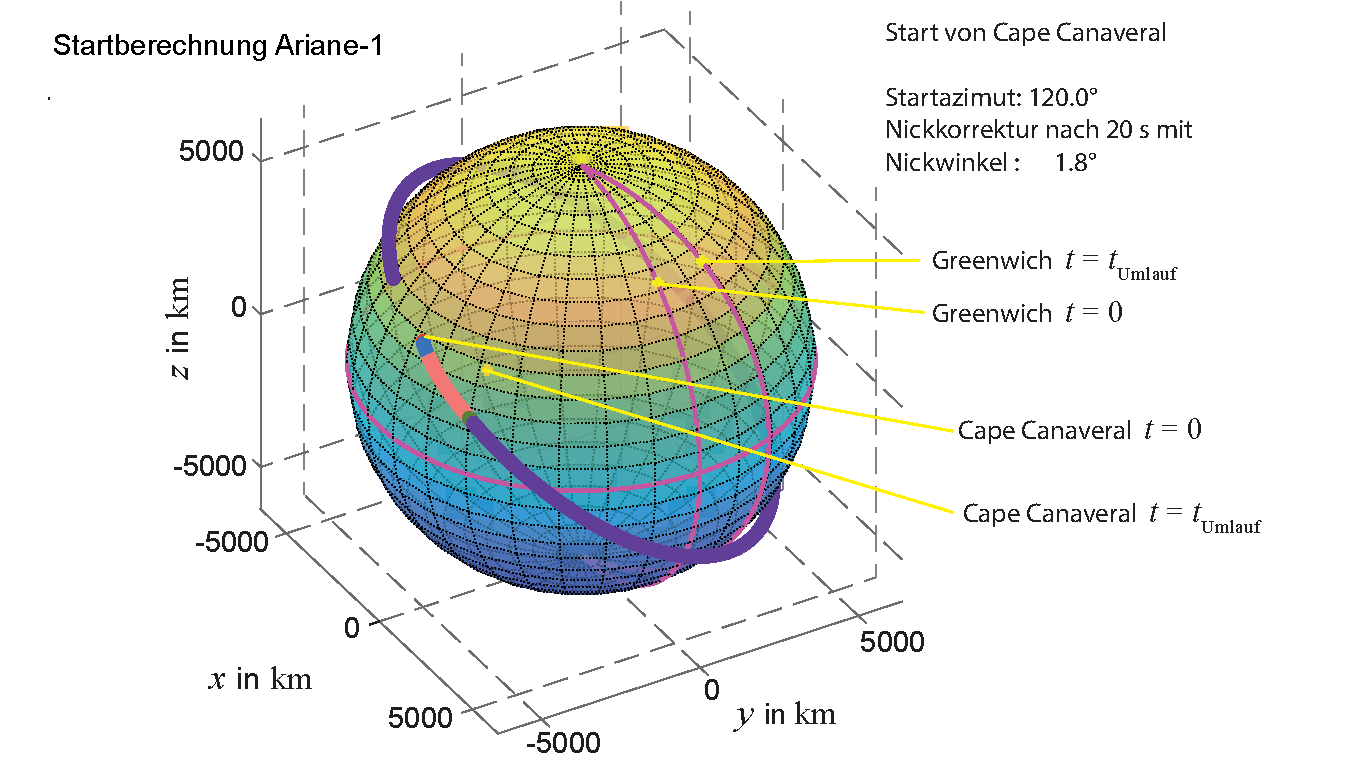
\includegraphics[width=\textwidth]{StartAriane01.pdf} 
	\caption[Trajektorie nach Start von der Erdoberfl�che.]{Trajektorie nach Start von der Erdoberfl�che. Parameter siehe \mladynref{Raketenstart2Orbit04.m}.}
	\label{abb:adyn_launch_lsg08}
\end{figure}

\begin{figure}[H]
	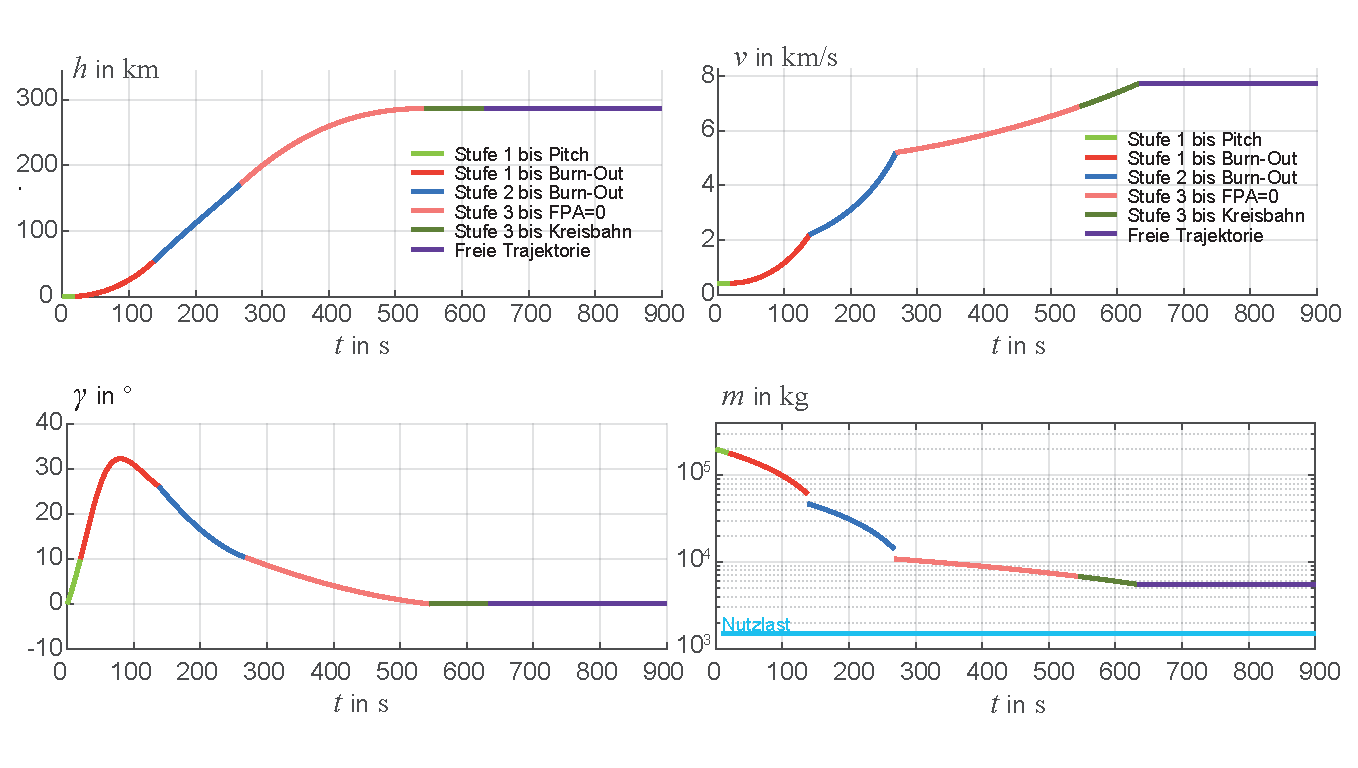
\includegraphics[width=\textwidth]{StartAriane02.pdf} 
	\caption[H�he, FPA,  Geschwindigkeit und  Masse der Ariane 1 nach Start von der Erdoberfl�che.]{H�he, FPA,  Geschwindigkeit und  Masse der Ariane 1 nach Start von der Erdoberfl�che. Parameter siehe \mladynref{Raketenstart2Orbit04.m}.}
	\label{abb:adyn_launch_lsg09}
\end{figure}

\item Als Alternative kann man die Trajektorien nat�rlich auch im mitbewegten \KOS des Beobachters im Horizontsystem berechnen. Das f�hrt auf �hnliche Rechnungen wie wir im Kap. 1.3.2 im Band I (Physik Bewegung) zum Wurf und freien Fall auf der Erdoberfl�che gemacht hatten.
\item Als weitere Alternative k�nnen wir nat�rlich das Ergebnis der Rechnungen im mitbewegten \KOS (Siehe Teilaufgabe 2) benutzen und ins Inertialsystem transformieren. Zwei Ortsvektoren sind dabei ausgezeichnet: Der Vektor zum Startpunkt und der Vektor zum aufsteigenden Knoten. Die Inklination und der aufsteigende Knoten der Bahn sind durch Startazimut, Startfenster und geographische Position des Startortes gegeben. Die Transformation erfolgt �ber die im \kap{hm_bahnen_hk_PQR} hergeleiteten Matrizen.\\
Wir empfehlen dem Leser zur Vervollst�ndigung des Bildes beide Alternativen selbst zu rechnen.
\end{enumerate}

\end{subprobs}
\end{sol} 
\textcolor{blue} {$\rightarrow$ zur} \probref{adyn_launch01}.\\
\noindent\rule[1ex]{\textwidth}{0.5pt}  \newpage  \clearpage

%-----------------------------------------------------------------------------------------------------------

\begin{sol}{prob:adyn_reentry01}\label{lsg:adyn_reentry01} %�bung27
\textbf{Parameter des Wiedereintritts in die Erdatmosph�re}\\

\begin{figure}[H]
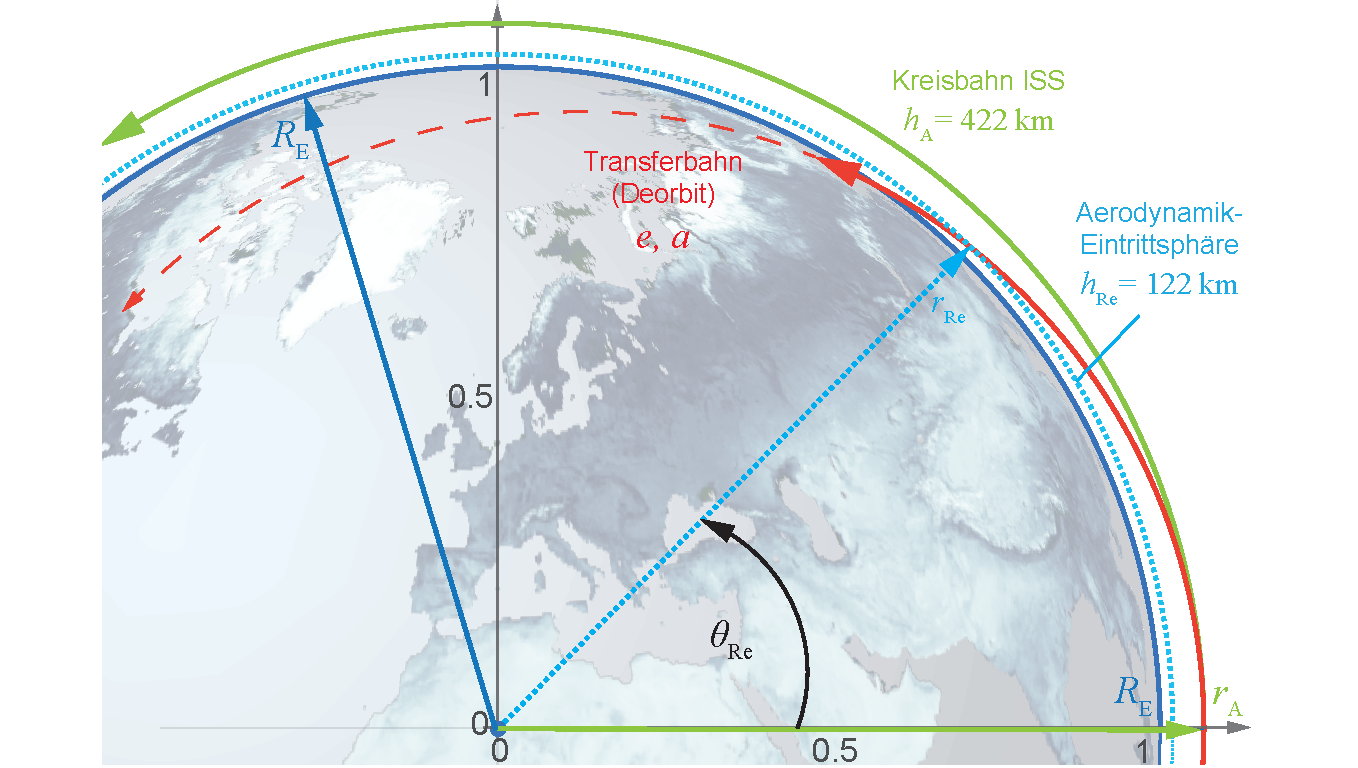
\includegraphics[width=\textwidth]{ReentryGeometrie01.pdf}
\caption[Geometrie des Wiedereintritts in die Erdatmosph�re.]{Geometrie des Wiedereintritts in die Erdatmosph�re. Siehe auch \mscr~\mladynref{Transfer2Reentry.m} f�r weitere Details und Graphiken.}
\label{abb:adyn_reentry_geometrie01}
\end{figure}

\begin{figure}[H]
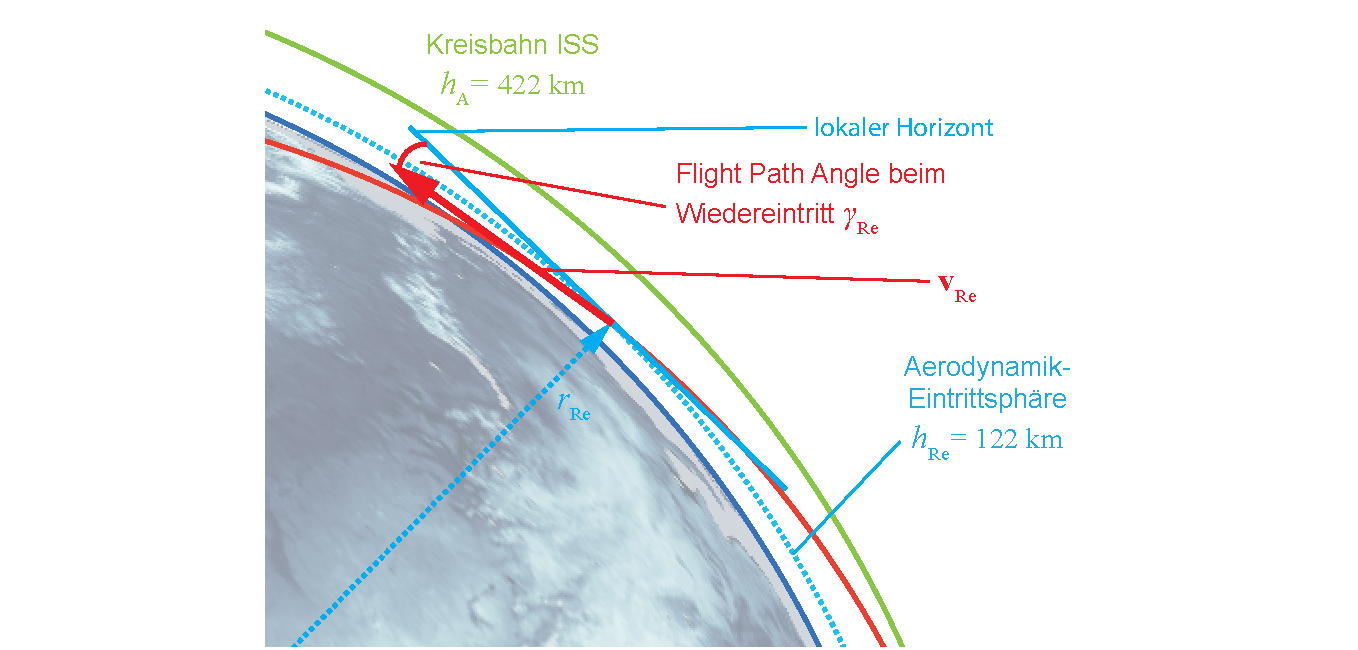
\includegraphics[width=\textwidth]{ReentryGeometrie02.pdf}
\caption[Geometrie des Wiedereintritts in die Erdatmosph�re.]{Geometrie  (Detail) des Wiedereintritts in die Erdatmosph�re. Siehe auch \mscr~\mladynref{Transfer2Reentry.m} f�r weitere Details und Graphiken.}
\label{abb:adyn_reentry_geometrie02}
\end{figure}

%\begin{nebenrechnung}
%\begin{align*}
    %e &= \frac{q^2-\lk 2q-1\rk\,\cos^2\gamma_\text{Re}}{q^2-\cos^2\gamma_\text{Re}} = \frac{q^2-\lk 2q-1\rk\,u^2}{q^2-u^2} \\
    %\cos\theta_\text{Re} &= q\,\frac{\lk 1-e\rk}{e}-\frac{1}{e} = \frac{q-1}{e}-q = \frac{Z}{N}\\
    %&= \frac{\lk q-1\rk\lk q^2-u^2\rk-q\,\lk q^2-\lk 2q-1\rk\,u^2\rk}{q^2-\lk2q-1\rk\,u^2}\\
    %N &= q^2-2\,q\,u^2+ u^2 = q^2-2q+1+2q-1-2\,q\,u^2+u^2\\
    %&= \lk q-1\rk^2 +\lk 2q-1\rk - \lk 2q-1\rk\,u^2 \\
    %&= \lk q-1\rk^2 + \lk2q-1\rk\lk1-u^2\rk \\
    %&= \hat{q}^2 + \lk 2q-1\rk\,\sin^2\gamma_\text{Re}\\
    %Z &=  \cancel{q^3} - \cancel{q\,u^2}-q^2+u^-\cancel{q^3} +2\,q^2\,u^2-\cancel{q\,u^2} = 2\,q^2\,u^2- 2\,q\,u^2 - q^2+u^2 \\
    %&= \lk q^2-2q+1\rk\,u^2 - \lk q^2-q^2\,u^2\rk = \hat{q}^2\,u^-q^2\,\lk1-u^2\rk\\
    %&= \hat{q}^2\,\cos^2\gamma_\text{Re} - q^2\,\sin^2\gamma_\text{Re}
%\end{align*}
%\end{nebenrechnung}

Wir haben die Geometrie des Deorbits in \figref{adyn_reentry_geometrie01} und \figref{adyn_reentry_geometrie02} dargestellt.\\
Gegeben sind $v_\text{A}$, $r_\text{A}$, $r_\text{Re}$ und der gew�nschte FPA $\gamma_\text{Re}$, gesucht sind der \anf{Ort} $\upsilon_\text{Re}$ \bzw $\theta_\text{Re}$ des \anf{Eintauchens} in die aerodynamische Zone/Sph�re und die Geschwindigkeit $v_\text{Re}$, die das Raumschiff dort hat. Dazu muss man die Bahnparameter $e$ \bzw $a$ kennen, f�r die gilt: $r_\text{A} = a\,\lk 1+e\rk$.\\
Wir starten mit Ellipsengleichung \eqref{eq:hm_kegelschnitt}:
\begin{align}
    r_\text{Re} = \frac{a\,\lk 1-e^2\rk}{1+e\,\cos\upsilon_\text{Re}} = \frac{a\,\lk1-e^2\rk}{1-e\,\cos\theta_\text{Re}} \,. \label{eq:adyn_lsg_reentry01}
\end{align}
Aus der vis-visa-Gleichung \eqref{eq:hm_vis-viva}, die wir zun�chst vektoriell aufschreiben aufschreiben, k�nnen wir eine Beziehung f�r $v_\text{Re}\lk r_\text{Re},\upsilon_\text{Re}\rk$ ableiten.
\begin{nebenrechnungNeu} {  }

\begin{align*}
   \text{Aus} ~~ \vec{L} \times\,\lk \vec{v}\times \vec{L}\rk &= \vec{v} \,\lk \vec{L}\vec{L}\rk - 			   \underbrace{\vec{L}\,\lk \vec{L}\vec{v}\rk}_{\substack{=0}} = L^2\,\vec{v} ~~
   \text{und}\\
    \vec{e} &= -\frac{1}{\mu}\,\lk \vec{L}\times \vec{v}\rk\,\frac{\vec{r}}{r}\,,~~~~
    \vec{v} = \frac{\mu}{L^2}\,\vec{L}\times\lk\vec{e} + \frac{\vec{r}}{r}\rk~~\text{folgt}\\
    \vec{L}\times \vec{v} &= -\mu\,\lk\frac{\vec{r}}{r}+\vec{e}\rk ~~\rightarrow~~
    \vec{L}\times\lk\vec{v}\times \vec{L}\rk = \vec{L}\times\mu\,\lk\frac{\vec{r}}{r} + \vec{e}\rk\,, \\
    L^2\,\vec{v} &= \mu\,\lek\vec{L}\times \lk\vec{e} + \frac{\vec{r}}{r}\rk\rek ~~\rightarrow~~~
    \vec{v} = \frac{\mu}{L^2}\lek \vec{L}\times\lk \vec{e}+ \frac{\vec{r}}{r}\rk\rek\,, \\
    \rightarrow~~~|\vec{v}| &=\frac{\mu}{L^2}\,\sqrt{\lek \vec{L}\times\lk \vec{e}+\frac{\vec{r}}{r}\rk\rek\lek\vec{L}\times\lk \vec{e}+\frac{\vec{r}}{r}\rk\rek}\,.\\
\text{Wegen}~~&\lk \vec{a}\times \vec{b}\rk\lk \vec{a}\times\vec{b}\rk = a^2\,b^2 -\lk a\,b\rk^2~~\text{folgt:}\\
    |\vec{v}| &= \frac{\mu}{L^2}\,\sqrt{L^2\,\lk \vec{e} + \frac{\vec{r}}{r}\rk^2 - \underbrace{\lek \vec{L}\,\lk \vec{e} + \frac{\vec{r}}{r}\rk\rek^2 }_{=0}}~~~\text{und da}~~~\vec{L} \perp \vec{e},\vec{r} \\
    |\vec{v}| &= \frac{\mu}{L^2}\,L\,\sqrt{\lk \vec{e} + \frac{\vec{r}}{r}\rk^2} = \frac{\mu}{L}\,\sqrt{e^2+2e\,\cos\upsilon_\text{e} +1}
\end{align*}
\end{nebenrechnungNeu}

Damit haben wir als zweite Gleichung:
\begin{align}
    v_\text{e} = \frac{\mu}{L}\,\sqrt{1+e\,\cos\upsilon_\text{Re} + e^2}\,. \label{eq:adyn_lsg_reentry02}
\end{align}
Als dritte Gleichung brauchen wir noch den FPA. Dieser ist gegeben durch den Winkel zwischen Geschwindigkeitsvektor $\vec{v}$ und lokalem Horizont.
Letzterer liegt senkrecht zum Radiusvektor (Abstandsvektor) $\vec{r}$ in der $\vec{r}$\,-\,$\vec{v}$-Bahnebene und stimmt mit der Richtung des Vektors $\vec{e}$ �berein.
Wir bilden das Skalarprodukt:
\begin{subequations}
\begin{align}
    \vec{v}\,\lk \frac{\vec{L}}{L}\times\frac{\vec{r}}{r}\rk &= r\,\dot{\upsilon} =v\,\cos\gamma\,, \label{eq:adyn_lsg_reentry03a}\\
    \vec{v}\,\frac{\vec{r}}{r} &= \dot{r} = \sin\gamma\,. \label{eq:adyn_lsg_reentry03b}
\end{align} \label{eq:adyn_lsg_reentry03}
\end{subequations}
Aus \eqref{eq:adyn_lsg_reentry03a} folgt mit \eqref{eq:adyn_lsg_reentry02} und $L = r^2\,\dot{\upsilon}$:
\begin{subequations}
\begin{align}
    \cos\gamma_\text{Re} = \frac{1+e\,\cos\upsilon_\text{Re}}{\sqrt{1+2e\,\cos\upsilon_\text{Re} + e^2}}\,,\label{eq:adyn_lsg_reentry04a} \\
    \sin\gamma_\text{Re} = \frac{e\,\sin\upsilon_\text{Re}}{\sqrt{1+2e\,\cos\upsilon_\text{Re}+e^2}}\,. \label{eq:adyn_lsg_reentry04b}
\end{align} 
\end{subequations}
Man kann folglich mit \eqref{eq:adyn_lsg_reentry04a} und  \eqref{eq:adyn_lsg_reentry04b} auch die Geschwindigkeit an einem beliebigen Bahnpunkt durch
\begin{align}
\begin{split}
    \vec{v} &= \frac{\mu}{L}
    \begin{pmatrix}
        \sin\gamma \\
        \cos\gamma
    \end{pmatrix}
    =
    \frac{\mu}{L}
    \begin{pmatrix}
        e\,\sin\upsilon \\
        1+e\,\cos\upsilon
    \end{pmatrix} \\
    &= \sqrt{\frac{\mu^{\killA{2}}}{\killA{\mu}\,a\,\lk 1-e^2 \rk}}
    \begin{pmatrix}
        e\,\sin\upsilon \\
        1+e\,\cos\upsilon
    \end{pmatrix} 
    =\sqrt{\frac{\mu}{p}}
     \begin{pmatrix}
        e\,\sin\upsilon \\
        1+e\,\cos\upsilon
    \end{pmatrix} 		
\end{split} \label{eq:adyn_lsg_reentry05}
\end{align}
in der Koordinate $\upsilon$ und den Bahnparametern $p$, $e$ ausdr�cken. \\
Zus�tzlich zu Gleichungen \eqref{eq:adyn_lsg_reentry01}, \eqref{eq:adyn_lsg_reentry02} und \eqref{eq:adyn_lsg_reentry04a} gilt noch $r_\text{A} = a\,\lk1+e\rk$ und $q= r_\text{A}/r_\text{Re} > 1$.
Aus \eqref{eq:adyn_lsg_reentry01} k�nnen wir dann folgende Beziehung ableiten:
\begin{align}
   e\,\cos\upsilon_\text{Re} &= \frac{a\,\lk 1-e^2\rk}{r_\text{Re}} -1 = \frac{a\,\lk 1+e\rk\lk 1-e\rk}{r_\text{Re}} = q\,\lk 1-e\rk-1 \,. \label{eq:adyn_lsg_reentry05a} 
\end{align}
Wir benutzen \eqref{eq:adyn_lsg_reentry05a} in \eqref{eq:adyn_lsg_reentry01} und erhalten:
\begin{align}
\begin{split}
    \cos\gamma_\text{Re} &= \frac{q\,\lk 1-e\rk}{\sqrt{1+2q\,\lk 1-e\rk -2+e^2}}
    = q\,\sqrt{\frac{\lk 1-e\rk^2}{2q-2\,e\,q-1+e^2}}\\
    &= q\,\sqrt{\frac{\lk 1-e\rk^2}{2q-2\,e\,q-\lk 1-e^2\rk}}
    = q\,\sqrt{\frac{\lk 1-e\rk^2}{2q\,\lk 1-e\rk - \lk 1+e\rk\lk1-e\rk}}
    = q\,\sqrt{\frac{1-e}{2q-\lk 1+e\rk}}
\end{split} \label{eq:adyn_lsg_reentry06} 
\end{align}
F�r $v_\text{Re}$ erhalten wir:
\begin{align}
\begin{split}
    v_\text{Re} &= \frac{\mu}{L}\,\sqrt{1+2e\,\cos\upsilon_\text{Re} +e} = \sqrt{\frac{\mu\,\lk 1+2q\,\lk 1-e\rk -1+e^2\rk}{r_\text{A}\,\lk 1-e^2\rk}}\\
    &= \sqrt{\frac{\mu}{r_\text{A}}}\,\sqrt{\frac{2q-2\,q\,e-1+e^2}{\lk 1+e\rk\lk 1-e\rk}} = \sqrt{\frac{\mu}{r_\text{A}}}\,\,\sqrt{\frac{2q\,\cancel{\lk 1-e\rk}}{\lk 1+e\rk\cancel{\lk 1-e\rk}} - \cancel{\frac{\lk 1-e^2\rk}{\lk 1+e\rk\lk1-e\rk}}} \\
    &= \sqrt{\frac{\mu}{r_\text{A}}}\,\sqrt{\frac{2q-\lk 1+e \rk}{\lk 1+e\rk}} = \sqrt{\frac{\mu}{r_\text{A}\,\lk 1+e\rk}}\,\sqrt{2q-\lk 1+e\rk}
\end{split}\label{eq:adyn_lsg_reentry07}
\end{align}
Aus \eqref{eq:adyn_lsg_reentry06} k�nnen wir die Exzentrizit�t $e$ bestimmen und dann $v_\text{Re}$ �ber \eqref{eq:adyn_lsg_reentry07}. 
\begin{align*}
\begin{split}
    \frac{u^2}{q^2} &= \frac{1-e}{2q-\lk 1+e\rk} ~~~~\text{mit}~~~~ u = \cos\gamma_\text{Re}\\ 
		u^2\,\lek 2q-\lk 1+e\rk\rek &= \lk 1-e\rk ~~\rightarrow~~
    \frac{u^2}{q^2}\,2q -\frac{u^2}{q^2}\,\lk 1\rk - \frac{u^2}{q^2}\,e^2 = 1-e \,,\\
    %\rightarrow~~\frac{u^2}{q^2}\,\lk 2q-1\rk -1 &= \frac{u^2}{q^2}\,e-1 = e\lk \frac{u^2}{q^2}-1\rk\\
    \rightarrow~~ e &= \frac{\lek \frac{u^2}{q^2}-\lk 2q-1\rk -1\rek}{\lek \frac{u^2}{q^2} -1\rek} = \frac{u^2\,\lk 2q-1\rk-q^2}{u^2-q^2} \\
    &= \frac{q^2-\cos^2\gamma_\text{Re}\,\lk 2q-1\rk}{q^2-\cos^2\gamma_\text{Re}}\,.
\end{split} 
\end{align*}
Mit der Beziehung f�r $e$, die man in \eqref{eq:adyn_lsg_reentry07} einsetzt, erh�lt man die Beziehungen \eqref{eq:adyn_reentry03} f�r $v_\text{Re}$ \bzw $\vec{v}_\text{Re}$ und �ber $\Delta \vec{v} = \vec{v}_\text{Re} - \vec{v}_\text{A}$, auch $|\Delta \vec{v}| =\Delta v$.

Wir vergleichen zum Schluss noch die Problemstellungen des Lambert-Transfers und des Wiedereintritt-Transfers miteinander:
\begin{table}[ht]
		\begin{center}
    \begin{tabular}{|L{2.5cm}|L{5cm}|}
    \hline
    \rule{0pt}{3pt}&  \\
    \rule{0pt}{6pt}\textit{Lambert-Problem} &  \\
 %   \rule{0pt}{3pt} &   \\
      Gegeben: & $r_1,\, r_2,\, \gamma = \angle (r_1,r_2),\, \Delta t$ \\
			Gesucht: & $a,\, e$,\, $v_\text{1,tr},\, \Delta v$ \\
    \rule{0pt}{3pt}&  \\
    \rule{0pt}{6pt}\textit{Deorbit-Transfer}& \\
%    \rule{0pt}{3pt}&  \\
      Gegegen: & $r_1, r_2,\, \text{FPA} =\gamma_\text{Re},\, v_\text{A}$ \\
			Gesucht: & $e,\, \upsilon_\text{Re} $,\, $v_\text{Re},\, \Delta v$ \\
    \rule{0pt}{3pt}&  \\
    \hline
    \end{tabular} 
		\end{center}
		\caption{Vergleich Lambert-Problem und Parameterbestimmung Reentry}
		\label{tab:adyn_vglLambertReentry}
\end{table}


\end{sol} 
\textcolor{blue} {$\rightarrow$ zur} \probref{adyn_reentry01}.\\
\noindent\rule[1ex]{\textwidth}{0.5pt}  \newpage  \clearpage

%-----------------------------------------------------------------------------------------------------------

\begin{sol}{prob:adyn_reentry02}\label{lsg:adyn_reentry02} %�bung28
\textbf{Auftrieb/Drag-Abh�ngigkeit bei Wiedereintritt in Erdatmosph�re}\\

Die Rechnung sind im \mscr~\mladynref{ReentryReal.m} im Detail hinterlegt.

\begin{figure}[H]
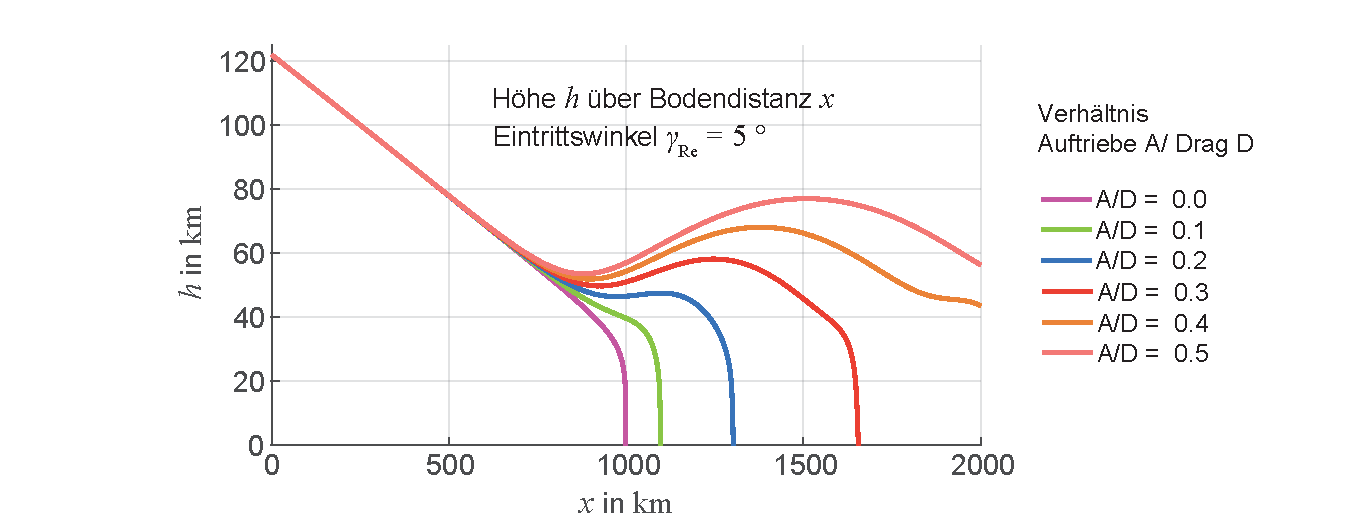
\includegraphics[width=\textwidth]{Reentry_Uebung01.pdf}
\caption[H�he $h$ nach Wiedereintritt in die Erdatmosph�re �ber die Bodendistanz $x$.]{H�he $h$ nach Wiedereintritt in die Erdatmosph�re �ber die Bodendistanz $x$ in Abh�ngigkeit vom Auftrieb/Drag-Verh�ltnis. Siehe \mscr~\mladynref{ReentryReal.m} f�r Parameter und Details.}
\label{abb:adyn_reentry_uebung01}
\end{figure}

\begin{figure}[H]
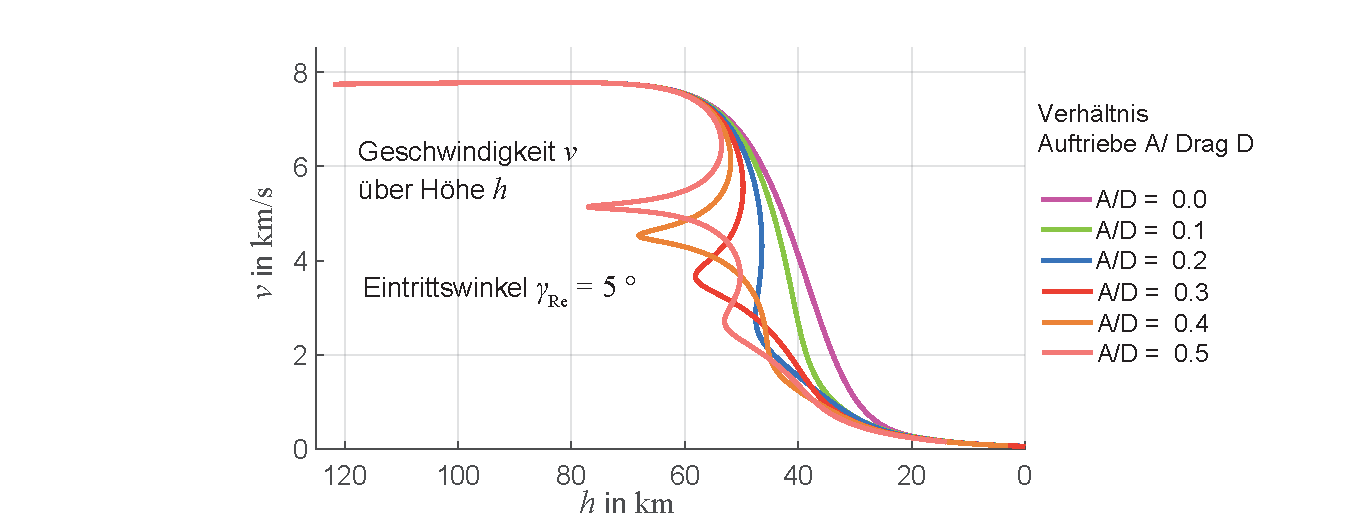
\includegraphics[width=\textwidth]{Reentry_Uebung02.pdf}
\caption[Geschwindigkeit $v$ nach Wiedereintritt in die Erdatmosph�re �ber die H�he $h$.]{Geschwindigkeit $v$ nach Wiedereintritt in die Erdatmosph�re �ber die H�he $h$ in Abh�ngigkeit vom Auftrieb/Drag-Verh�ltnis. Siehe \mscr~\mladynref{ReentryReal.m} f�r Parameter und Details.}
\label{abb:adyn_reentry_uebung02}
\end{figure}

\begin{figure}[H]
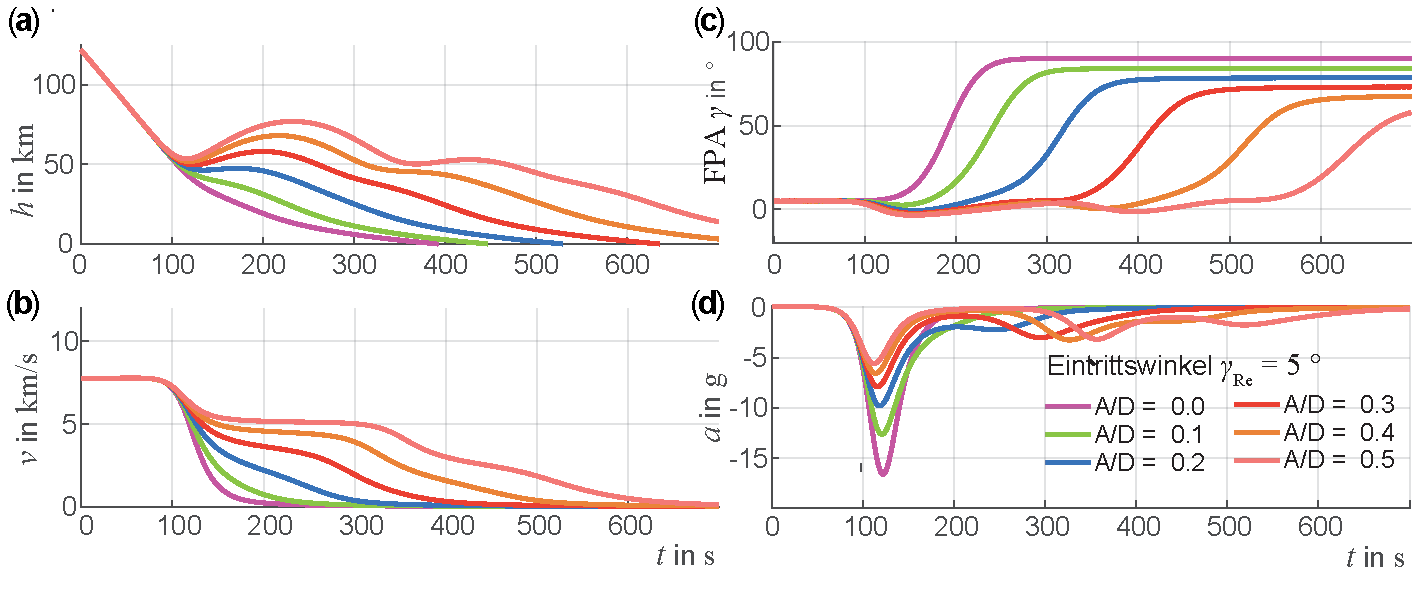
\includegraphics[width=\textwidth]{Reentry_Uebung03.pdf}
\caption[Verschieden Parameter nach Wiedereintritt als Funktion der Zeit.]{H�he $h$ \fa, Geschwindigkeit $v$ \fb, Flight Path Angle FPA \fc und Beschleunigung $a$ \fd nach Wiedereintritt in die Erdatmosph�re �ber die Zeit $t$ in Abh�ngigkeit vom Auftrieb/Drag-Verh�ltnis. Siehe \mscr~\mladynref{ReentryReal.m} f�r Parameter und Details.}
\label{abb:adyn_reentry_uebung03}
\end{figure}

\end{sol} 
\textcolor{blue} {$\rightarrow$ zur} \probref{adyn_reentry02}.\\
\noindent\rule[1ex]{\textwidth}{0.5pt}  \newpage  \clearpage

%-----------------------------------------------------------------------------------------------------------

\begin{sol}{prob:adyn_reentry03}\label{lsg:adyn_reentry03} %�bung29
\textbf{Normierte Gleichungen f�r $v(h)$ und $\gamma(h)$ bei Wiedereintritt}\\

F�r den Fall $F_\text{S}=0$ (was \zb f�r das Space Shuttle oft nicht erf�llt ist!) starten wir von:
\begin{subequations}
    \begin{align}
        \dot{v} &= -\frac{F_\text{D}}{m_\text{R}} - g\lk h\rk\,\sin\gamma = -v^2\,\frac{K_\text{D}}{H_0}\,\e^{-\frac{h}{H_0}}-g\,\sin \gamma\,,\\
        v\,\dot{\gamma} &= -\frac{F_\text{A}}{m_\text{R}} + \lk g\lk h\rk  - \frac{v^2}{r}\rk\,\cos\gamma\,,\\
        \dot{h} &= -v\,\sin\gamma\,,\\
        \dot{x} &= v\,\cos\gamma\,. 
    \end{align} \label{eq:adyn_normierte01}
\end{subequations}

Wir benutzen die barometrische H�henformel, sowie folgende Beziehungen f�r dem Drag und den Auftrieb:
\begin{subequations}
    \begin{align}
        F_\text{D} &= \frac{1}{2}\,\varrho\lk h\rk \,v^2\,C_\text{D}\,A_\text{R} = m_\text{R}\,v^2\,\frac{\kappa_\text{D}}{H_0}\,\e^{-\frac{h}{H_0}}\,,\\
        F_\text{A} &= \frac{1}{2}\,\varrho\lk h\rk \,v^2\,C_\text{A}\,A_\text{R} = m_\text{R}\,v^2\,\frac{\kappa_\text{A}}{H_0}\,\e^{-\frac{h}{H_0}}\,.
    \end{align} \label{eq:adyn_normierte02}
\end{subequations}

F�r $g\lk h\rk$ setzen wir an:
\begin{align}
    g\lk h\rk = g_0\,\frac{R_\text{E}{}^2}{r^2} = g_0\,\frac{R_\text{E}{}^2}{\lk R_\text{E}+h\rk^2}\,.  \label{eq:adyn_normierte03}
\end{align}
Wir normalisieren nun das DGL-System mit:
\begin{align}
    \begin{split}
        \mu &= \frac{v}{v_\text{K}} = \frac{v}{\sqrt{g_0\,R_\text{E}}} = \frac{v}{\sqrt{G\,M_\text{E}}}\\
        \eta &= \frac{h}{H_0}\,, ~~~~~~~~ \tau = \frac{g_0}{v_\text{K}}\,t\,, ~~~~~~~~
        \chi= \frac{x}{H_0}\, \\
        \D\tau &= \frac{g_0}{v_\text{K}}\,\D t\,, ~~~~~~~~ \D t = \frac{v_\text{K}}{g_0}\,\D \tau
    \end{split}\label{eq:adyn_normierte04}
\end{align}
und erhalten:
\begin{subequations}
    \begin{align}
        \begin{split}
            \frac{\D}{\D t}\,v &= -v^2\,\frac{\kappa_\text{D}}{H_0}\,\e^{-\frac{h}{H_0}} +g_0\,\frac{R_\text{E}{}^2}{r^2}\,\sin\gamma ~~~
            \rightarrow ~~~ \frac{\D}{\D \tau}\,\mu = -\mu^2\,\kappa_\text{D}\,\frac{R_\text{E}}{H_0}\,\e^{-\eta} +\sin\gamma\,.
          \end{split}
          \label{eq:adyn_normierte05a}
    \end{align}
und
    \begin{align}
        \begin{split}
            v\,\frac{\D}{\D t}\,\gamma &= -v^2\,\frac{\kappa_\text{A}}{H_0}\,\e^{-\frac{h}{H_0}} +\lk g-\frac{v^2}{r}\rk\,\cos\gamma~~~
            \rightarrow ~~~~ \mu\,\frac{\D}{\D\tau}\,\gamma =  -\mu^2\,\kappa_\text{D}\,\frac{A}{D}\,\frac{R_\text{E}}{H_0}\,\e^{-\eta} +\lk 1-\mu^2\rk\,\cos\gamma\,. 
          \end{split}
          \label{eq:adyn_normierte05b}
    \end{align}\label{eq:adyn_normierte05}
\end{subequations}
Die Gleichungen f�r H�he und Bodendistanz werden einfach zu:
\begin{subequations}
    \begin{align}
      \frac{\D}{\D\tau}\,\eta
      & = -\frac{R_\text{E}}{H_0}\, \mu\,\sin\gamma\,,
        \label{eq:adyn_normierte06a}\\
      \frac{\D}{\D\tau}\,\chi
      & = +\frac{R_\text{E}}{H_0}\,\mu\,\cos\gamma\,. \label{eq:adyn_normierte06b}
    \end{align} 
\end{subequations}

Wir setzen jetzt $\hat{\epsilon} = \mu^2$ und $\hat{\eta} = 2\,\frac{\kappa_\text{D}}{\sin\gamma_\text{Re}}\,\e^{-\eta}$ in \eqref{eq:adyn_normierte05} ein und erhalten mit der Substitution $\D \tau \rightarrow \D \hat{\eta} $ (siehe Nebenrechnung):
\begin{subequations}
  \begin{align}
    \frac{\D\lk \ln \hat{\epsilon}\rk}{\D \hat{\eta}}
    &= - \frac{\sin\gamma_\text{Re}}{\sin\gamma}
      + \frac{2H_0}{\hat{\epsilon}\,\hat{\eta}\,R_\text{E}}\,,
      \label{eq:adyn_normierte07a}\\
    \frac{\D\lk \cos\gamma\rk}{\D \hat{\eta}}
    &= \frac{\sin\gamma_\text{Re}}{2}\,\frac{A}{D}
      - \lk \frac{1}{\hat{\epsilon}}-1 \rk \,\frac{H_0\,\cos\gamma}
      {\hat{\eta}\,R_\text{E}}\,.
      \label{eq:adyn_normierte07b}
  \end{align}\label{eq:adyn_normierte07}
\end{subequations}

Die erste Gleichung ist eine Gleichung f�r die Entwicklung der (dimensionslosen) Energie $\hat{\epsilon}$ als Funktion der (dimensionslosen) H�he $\hat{\eta}$ und die zweite eine des FPA $\gamma$ ebenfalls als Funktion der H�he.

\begin{nebenrechnungNeu}  {  }

  Zun�chst nehmen wir uns \eqref{eq:adyn_normierte07a} vor.
  Wir beginnen mit der Ableitung und ber�cksichtigen die eingef�hrten
  Koordinatentransformationen, die eine mehrfache Verkettung enthalten,
  \begin{equation}
    \frac{\D\lk \ln \hat{\epsilon}(\tau(\eta(\hat{\eta})))\rk}{\D \hat{\eta}}
    = \frac{\D \eta}{\D \hat{\eta}} \frac{\D\lk \ln \hat{\epsilon}
      (\tau(\eta))\rk}{\D \eta}
    = \frac{\D \eta}{\D \hat{\eta}} \frac{\D \tau}{\D \eta}
    \frac{\D\lk \ln \hat{\epsilon}(\tau)\rk}{\D \tau} \; .
  \end{equation}
  Um die Ableitung berechnen zu k�nnen, ben�tigen wir also die Umkehrungen
  der Koordinatentransformation
  \begin{equation*}
    \hat{\eta} = 2\,\frac{\kappa_\text{D}}{\sin\gamma_\text{Re}}\,\e^{-\eta}
    \qquad \to \qquad \eta = -\ln\lk \frac{\sin\gamma_\text{Re}}
    {2\,\kappa_\text{D}}\, \hat{\eta} \rk
  \end{equation*}
  \begin{subequations}
    und daraus
    \begin{equation}
      \frac{\D \eta}{\D \hat{\eta}} = - \frac{\D}{\D \hat{\eta}} \ln\lk
      \frac{\sin\gamma_\text{Re}}{2\,\kappa_\text{D}}\, \hat{\eta} \rk
      = -\frac{1}{\hat{\eta}}
      \label{eq:adyn_normierte08a}
    \end{equation}
    Weiterhin kennen wir aus \eqref{eq:adyn_normierte06a} $\D\eta / \D \tau$
    und berechnen
    \begin{equation}
      \frac{\D \tau}{\D \eta} = \frac{1}{\D \eta/\D \tau} = - \frac{H_0}
      {R_\mathrm{E}}\frac{1}{\mu \sin\gamma} \; .
      \label{eq:adyn_normierte08b}
    \end{equation}
  \end{subequations}
  Schlie�lich ber�cksichtigen wir noch
  \begin{equation}
    \frac{\D\lk \ln \hat{\epsilon}(\tau)\rk}{\D \tau}
    = \frac{\D\lk \ln \mu(\tau)^2 \rk}{\D \tau}
    = 2 \frac{\D\lk \ln \mu(\tau) \rk}{\D \tau}
    = \frac{2}{\mu} \frac{\D \mu(\tau)}{\D \tau} \; .
    \label{eq:adyn_ablLnEpsilon}
  \end{equation}
  Wir fassen nun \eqref{eq:adyn_ablLnEpsilon} mit den Ableitungen
  \eqref{eq:adyn_normierte08a} und \eqref{eq:adyn_normierte08b} zusammen,
  \begin{equation}
     \frac{\D\lk \ln \hat{\epsilon}\rk}{\D \hat{\eta}} 
     = \frac{2}{\hat{\eta}\,\mu^2\, \sin\gamma} \frac{H_0}{R_\mathrm{E}}
     \frac{\D \mu(\tau)}{\D \tau} \; ,
  \end{equation}
  und erhalten durch das Einsetzen von \eqref{eq:adyn_normierte05a}
  \begin{multline}
     \frac{\D\lk \ln \hat{\epsilon}\rk}{\D \hat{\eta}}
     = \frac{2}{\hat{\eta}\,\mu^2\, \sin\gamma} \frac{H_0}{R_\mathrm{E}}
     \lk -\mu^2\,\kappa_\text{D}\, \frac{R_\text{E}}{H_0}\,\e^{-\eta}
     +\sin\gamma \rk
     = -\frac{1}{\hat{\eta}}\, \frac{\sin\gamma_\text{Re}}{\sin\gamma}\,
     \underbrace{\frac{2\,\kappa_\text{D}}{\sin\gamma_\text{Re}}\e^{-\eta}
     }_{\hat{\eta}} + \frac{H_0}{R_\mathrm{E}} \frac{1}{\hat{\eta}\,\mu^2} \\
     = -\frac{\sin\gamma_\text{Re}}{\sin\gamma}
     + \frac{H_0}{\hat{\epsilon}\,\hat{\eta} \,R_\text{E}} \; .
  \end{multline}

  Vollkommen analog berechnen wir
  \begin{equation}
    \frac{\D\lk \cos \gamma(\tau(\eta(\hat{\eta})))\rk}{\D \hat{\eta}}
    = \frac{\D \eta}{\D \hat{\eta}} \frac{\D\lk \cos \gamma(\tau(\eta))\rk}
    {\D \eta}
    = \frac{\D \eta}{\D \hat{\eta}} \frac{\D \tau}{\D \eta}
    \frac{\D\lk \cos \gamma(\tau)\rk}{\D \tau} 
    = - \frac{\D \eta}{\D \hat{\eta}} \, \frac{\D \tau}{\D \eta} \,
    \sin\gamma \, \frac{\D \gamma(\tau)}{\D \tau} \; ,
  \end{equation}
  wobei wir wieder die Ableitungen \eqref{eq:adyn_normierte08a} und
  \eqref{eq:adyn_normierte08b} einsetzen und \eqref{eq:adyn_normierte05b}
  verwenden,
  \begin{multline}
    \frac{\D\lk \cos \gamma \rk}{\D \hat{\eta}}
    = -\frac{1}{\hat{\eta}\,\mu^2} \frac{H_0}{R_\mathrm{E}}\,
    \lk -\mu^2\,\kappa_\text{D}\,\frac{A}{D}\, \frac{H_0}{R_\mathrm{E}} \,
    \frac{R_\text{E}}{H_0}\,\e^{-\eta} +\lk 1-\mu^2\rk\,\cos\gamma \rk \\
    = \frac{1}{\hat{\eta}} \, \frac{A}{D}\, \frac{\sin\gamma_\text{Re}}{2}\,
    \underbrace{\frac{2\,\kappa_\text{D}} {\sin\gamma_\text{Re}}\e^{-\eta}
    }_{\hat{\eta}}
    - \frac{H_0}{R_\mathrm{E}}\, \lk \frac{1}{\mu^2} - 1 \rk \frac{\cos\gamma}
    {\hat{\eta}} \\
    = \frac{\sin\gamma_\text{Re}}{2}\, \frac{A}{D}
    - \lk \frac{1}{\hat{\epsilon}} - 1 \rk \frac{H_0\,\cos\gamma}{\hat{\eta}\,
      R_\text{E}} \; .
  \end{multline}

\end{nebenrechnungNeu}

\end{sol} 
\textcolor{blue} {$\rightarrow$ zur} \probref{adyn_reentry03}.\\
\noindent\rule[1ex]{\textwidth}{0.5pt}  \newpage  \clearpage

%-----------------------------------------------------------------------------------------------------------

\begin{sol}{prob:adyn_reentry04}\label{lsg:adyn_reentry04} %�bung30
\textbf{ISS Stabilit�t - Absturz und Vergl�hen des Satelliten Tiangong-1}\\

\begin{figure}[H]
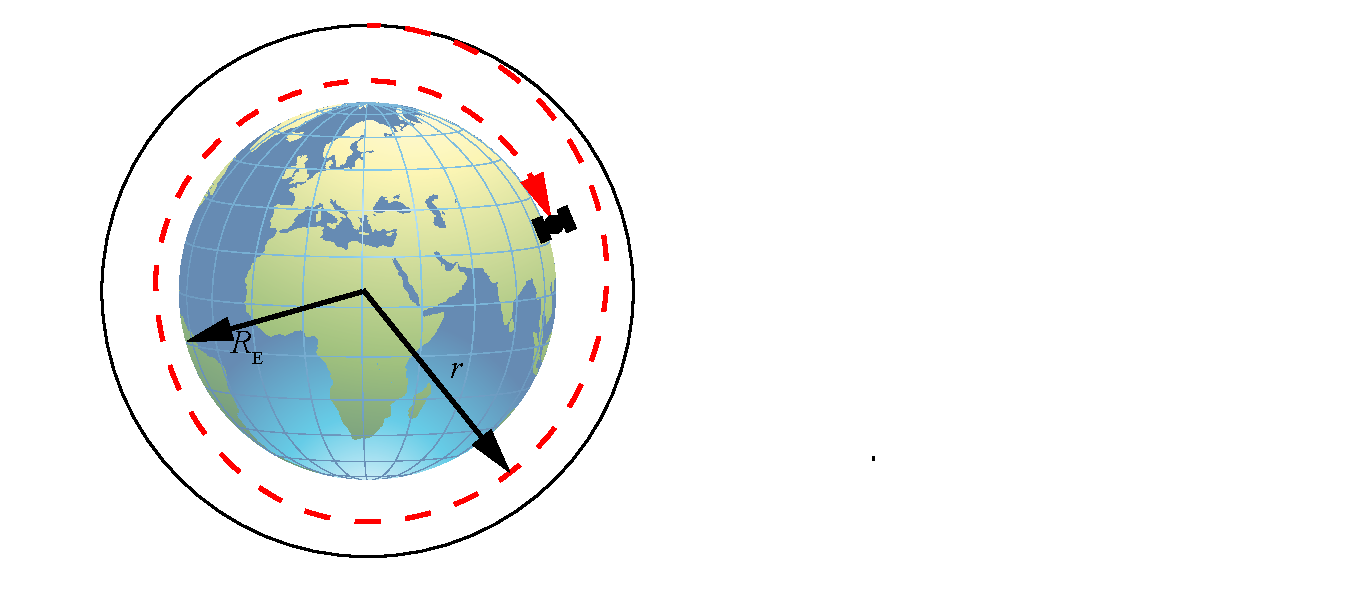
\includegraphics[width=\textwidth]{Tiangong01.pdf}
\caption[Einfaches Modell zur Berechnung des Absturzes des chinesischen Satelliten Tiangong-1.]{Einfaches Modell zur Berechnung des Absturzes des chinesischen Satelliten Tiangong-1.}
\label{abb:adyn_Tiangong01}
\end{figure}


\begin{enumerate}
\item [1.] Wir k�nnen aus \figref{adyn_ISS2004} folgende Raten des Radiusabfalls f�r das Jahr 2014 bestimmen: \\
    \begin{align*}
        \frac{\Delta a}{\Delta t} &= \SI{-1.578e-6}{\km\per\second} \pm \SI{1.0e-6}{\km\per\second} \approx \SI{-130}{\metre\per\day}\pm \SI{80}{\metre\per\day}
    \end{align*}
    Daraus erh�lt man �ber \eqref{eq:adyn_tiangong03} und \eqref{eq:adyn_tiangong05} eine effektive Fl�che 
    \begin{align*}
        A_\text{eff} = \kappa_\text{D}\,A_\perp \approx \SI{210}{\square\metre} \pm \SI{140}{\square\metre}\,,
    \end{align*}
    was eher am unteren Ende der Erwartung liegt, wenn man
    \begin{align*}
        A_\perp \approx
        \begin{cases}
            \SI{50}{\metre}\cdot\SI{70}{\metre} = \SI{3500}{\square\metre}\\
            \SI{109}{\metre}\cdot\SI{51}{\metre} \approx \SI{5000}{\square\metre}
        \end{cases}
    \end{align*}
    entsprechend der Literatur ansetzt, wobei man hierbei das Sonnensegel als voll ausgebreitet in Flugrichtung annimmt. Wir m�ssten dann von einem relativ niedrigen $\kappa_\text{D}$ Wert von $\SI{0.1}{}$ ausgehen. \\
    Fehler in unserer Absch�tzung k�nnen vor allem in der Dichteberechnung liegen. Eine �berpr�fung mit dem Harries-Priester-Modell \cite{Montenbruck2012} ergibt f�r eine H�he von $\SI{420}{\km}$ Werte von $\varrho$ zwischen $\SI{1.558}{\g\per\cubic\km}$ und $\SI{5.684}{\g\per\cubic\km}$ je nach Tageszeit eine etwas bessere �bereinstimmung mit den $A_\text{eff}$-Werten aus der Literatur!\\
    Im Fall eines Magnetsturms kann man von einer Zunahme der Partikeldichte ausgehen, die wegen
    \begin{align*}
        \frac{\Delta a_1/\Delta t}{\Delta a_0/\Delta t} = 4 = \frac{\varrho_1}{\varrho_0}
    \end{align*}
    in etwa proportional zur Zunahme der Rate des Radiusabfalls ist. \\
\item [2.] Wir k�nnten zur Berechnung nat�rlich das Instrumentarium aus \kap{adyn_reentry} benutzen und da insbesondere die Gleichungen \eqref{eq:adyn_reentry02} \bzw \eqref{eq:adyn_reentry02}. Da uns aber wesentliche Informationen fehlen \bzw nicht in ausreichender Genauigkeit vorliegen, wollen wir ein einfaches Modell verwenden. Wir gehen von einer kreisf�rmigen Bahn aus, nehmen an, dass der Drag immer entgegengesetzt zur Richtung der Geschwindigkeit wirkt. Ebenso wird ein konstanter FPA von $\gamma=0$ angenommen. Damit k�nnen wir auch annehmen, dass die Verringerung der Energie des Satelliten (\figref{adyn_Tiangong01}) allein aus der Reibungsarbeit des Drags resultiert, also
    \begin{align}
        \frac{\D}{\D t} H = \frac{\D}{\D t}\lk \frac{\mu_\text{E}\,m_\text{R}}{2r}\rk = F_\text{D}\,v_\text{R}~~~\text{mit}~~~
        F_\text{D} = \frac{1}{2}\,\varrho\lk r\rk \,\kappa_\text{D}\,A_\perp\,v_\text{R}{}^2\,,\label{eq:adyn_tiangong01}
    \end{align}
    worin $\varrho\lk r\rk$ die Dichte der Restatmosph�re im Abstand $r$ vom Erdmittelpunkt und $A_\perp$ die wirksame Fl�che des Raumschiffs senkrecht zur Bewegungsrichtung ist, $\kappa_\text{D}$ ist der Drag-Koeffizient. \\
    Wir erhalten aus \eqref{eq:adyn_tiangong01} die einfache Differentialgleichung 
    \begin{align}
        \begin{split}
            \dot{r} &= -\kappa_\text{eff}\,\sqrt{r}\,\varrho\lk r\rk ~~~~ \text{\bzw mit} ~~~~ r = h + R_\text{E}\, \\
            \dot{h} &= -\kappa_\text{eff}\,\sqrt{h+R_\text{E}}\,\varrho\lk h\rk ~~~~ \text{und}~~~\kappa_\text{eff} = \sqrt{\mu_\text{E}}\,\frac{\kappa_\text{D}\,A_\perp}{m_\text{R}}\,.
        \end{split} \label{eq:adyn_tiangong03}
    \end{align}
    F�r $\varrho\lk h\rk$ benutzen wir ein Modell der Australian Space Weather Agency \cite{Fiolhais2023}:
    \begin{align}
        \varrho\lk h\rk = \SI{6e-1}{} \exp\lk-\frac{\lk h-h_0\rk}{H}\rk\,\SI{}{\kg\per\cubic\km}\label{eq:adyn_tiangong04}
    \end{align}
    mit $H= 29.5 \pm 0.1$ und h=\SI{175}{ \km}.\\
    Da $m_\text{R} = \SI{8.5e3}{\kg}$ bekannt ist, ist der einzig anzupassende Parameter in unserem Modell dann die effektive Fl�che $A_\text{eff} = \kappa_\text{D}\,A_\perp$:
    \begin{align}
        \kappa_\text{eff} = \sqrt{\mu_\text{E}}\,\frac{A_\text{eff}}{m_\text{R}} = \sqrt{\mu_\text{E}}\,\frac{\kappa_\text{D}\,A_\perp}{m_\text{R}}\,. \label{eq:adyn_tiangong05}
    \end{align}
    Wenn wir mit den Anfangswerten f�r Apog�um und Perig�um von $\SI{286}{\km}$ \bzw $\SI{274}{\km}$ eine Anpassung an die experimentellen Werte vornehmen, erhalten wir $A_\text{eff,A} \approx \SI{63}{\square\metre}$ \bzw $A_\text{eff,P} \approx \SI{33}{\square\metre}$, was mit den Abmessungen der Raumstation von $\SI{4}{\metre}\cdot\SI{10}{\metre}$ relativ gut �bereinstimmt (\figref{adyn_Tiangong02}). Gleichwohl ist der Unterschied zwischen den Perig�ums- und Apog�umswerten recht gro�, was aber an unserem einfachen Modell liegt. \\
    Der Leser �berlege sich, ein verbessertes (numerisches) Modell, welches die Elliptizit�t der Anfangsbahn ber�cksichtigt und den Drag dann st�ckweise auf der elliptischen Bahn ber�cksichtigt. Welche weiteren Verbesserungen des Modells sind dar�ber hinaus denkbar und relativ einfach umzusetzen?\\

\begin{figure}[H]
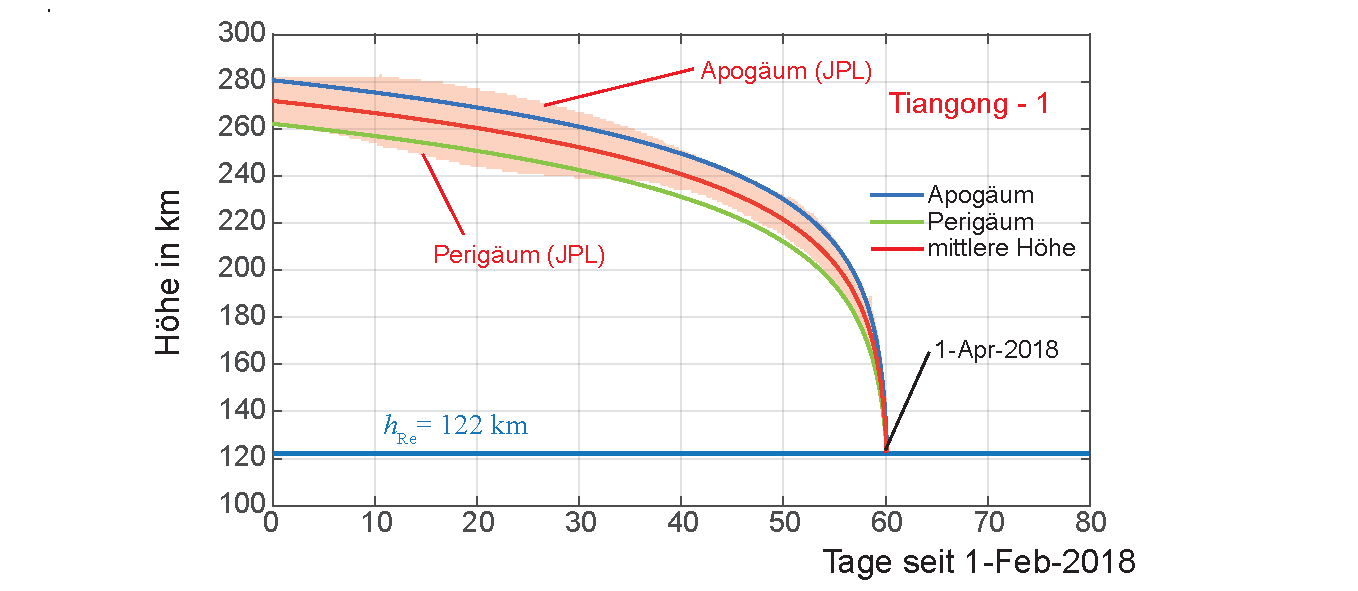
\includegraphics[width=\textwidth]{Tiangong02.pdf}
\caption[Zeitliche Entwicklung des Bahnradius bis zum Absturz des chinesischen Satelliten Tiangong-1.]{Zeitliche Entwicklung des Bahnradius des chinesischen Satelliten Tiangong-1.}
\label{abb:adyn_Tiangong02}
\end{figure}

\end{enumerate}    

Alle Rechnungen sind im \mscr~\mladynref{OrbitalDecay.m} hinterlegt. 

\end{sol} 
\textcolor{blue} {$\rightarrow$ zur} \probref{adyn_reentry04}.\\
\noindent\rule[1ex]{\textwidth}{0.5pt}  \newpage  \clearpage

%-----------------------------------------------------------------------------------------------------------

\begin{sol}{prob:adyn_BoatRocketModel}\label{lsg:adyn_BoatRocketModel} %�bung31
\textbf{Zur Entspannung}\\

Die anf�ngliche Gesamtmasse $M$ besteht aus der Boot- und K�rpermasse $m_\text{B},\, m_\text{L}$, sowie den $N$ Kokosn�ssen mit der Masse $m_\text{K}$ pro Nuss.
    \begin{align}
        M &= m_\text{L} + m_\text{B} + \sum\limits_1^N m_\text{K} \,. \label{eq:adyn_RaketenAlt01}
    \end{align}
F�r jeden Abwurf einer Kokosnuss schreiben wir sukzessive die Geschwindigkeit $V_i$ des Bootes nach Abwurf einer Kokosnuss �ber die Impulserhaltung auf:\\
\underline{1. Abwurf:} 
    \begin{align}
        -m_\text{K}\,v_\text{K} + \lk M-m_\text{K}\rk \,V_1 &= 0 ~~~~
        \rightarrow  ~~~~~ V_1 &= \frac{m_\text{K}}{M-m_\text{K}}\,v_\text{K}\label{eq:adyn_RaketenAlt02}
    \end{align}\\
\underline{2. Abwurf:} 
    \begin{align}
        -m_\text{K}\,\lk v_\text{K} - v_1\rk + \lk M-2m_\text{K}\rk\,V_2 &= \lk M-m_\text{K}\rk\,V_1 ~~~~
        \rightarrow ~~~~ V_2 &= \lek \frac{m_\text{K}}{M-m_\text{K}} + \frac{m_\text{K}}{M-2m_\text{K}}\rek\,v_\text{K} \label{eq:adyn_RaketenAlt03}  
    \end{align}\\
\underline{N-te Abwurf} 
    \begin{align}
        V_N = \sum\limits_{n=1}^N \frac{m_\text{K}\,v_\text{K}}{M-n\,m_\text{K}} = \frac{m_\text{K}\,v_\text{K}}{M}\,\sum\limits_{n=1}^N\,\frac{1}{1-n\,\frac{m_\text{K}}{M}}\label{eq:adyn_RaketenAlt04}  
    \end{align}

Man kann leicht mit \matlab{} zeigen, dass diese Summe konvergiert. Man beachte dabei, dass $N\,m_\text{K} = M-m_\text{L} - m_\text{B}$ ist. \\
F�hren wir die Masse $m_\text{G} = n\,m_\text{K}$ als die Masse der geworfenen Kokosn�sse ein, 
\begin{align}
    V_n &= v_\text{K}\,\sum\limits_{n=1}^N\,\frac{1}{\mu^N-n} ~~~~ \text{mit} ~~~~ \mu = \frac{n\,M_0}{M_\text{T}} = \frac{n\,M_0}{n\,m_\text{K}} ~~~~ \rightarrow ~~~~ \mu = \frac{M_0}{m_\text{K}}>1 \nonumber \\
    &= v_\text{K}\,\lek \frac{1}{\mu-1}+\frac{1}{\mu-2} + \ldots +\frac{1}{\mu-n}\rek \label{eq:adyn_RaketenAlt05}  
\end{align}
Wir bilden nun den Grenzwert:
\begin{align}
    \lim_{N\to\infty} V_N = v_\text{K}\, \lim_{N\to\infty}\sum\limits_{n=1}^N\,\frac{1}{\mu-n}\label{eq:adyn_RaketenAlt06}\,.
\end{align}
Im \mscr ~ \mladynref{AlternativRaketenGL.m} l�sst sich die Grenzwertbildung gut numerisch simmulieren. Das Ergebnis ist in \figref{adyn_RaketenAlternative} gezeigt.\\
Wir ersetzen $\mu = n\,M_0/M_\text{T} = n/x$ mit $0<x=M_\text{T}/M_0<1$:
\begin{align}
    V_N = v_\text{K}\sum\limits_{n=1}^N\,\frac{1}{n/x-n}\,\frac{x}{x} = v_\text{K}\sum\limits_{n=1}^N\,\frac{x}{n-n\,x}\label{eq:adyn_RaketenAlt07}\,.
\end{align}

\begin{figure}[H]
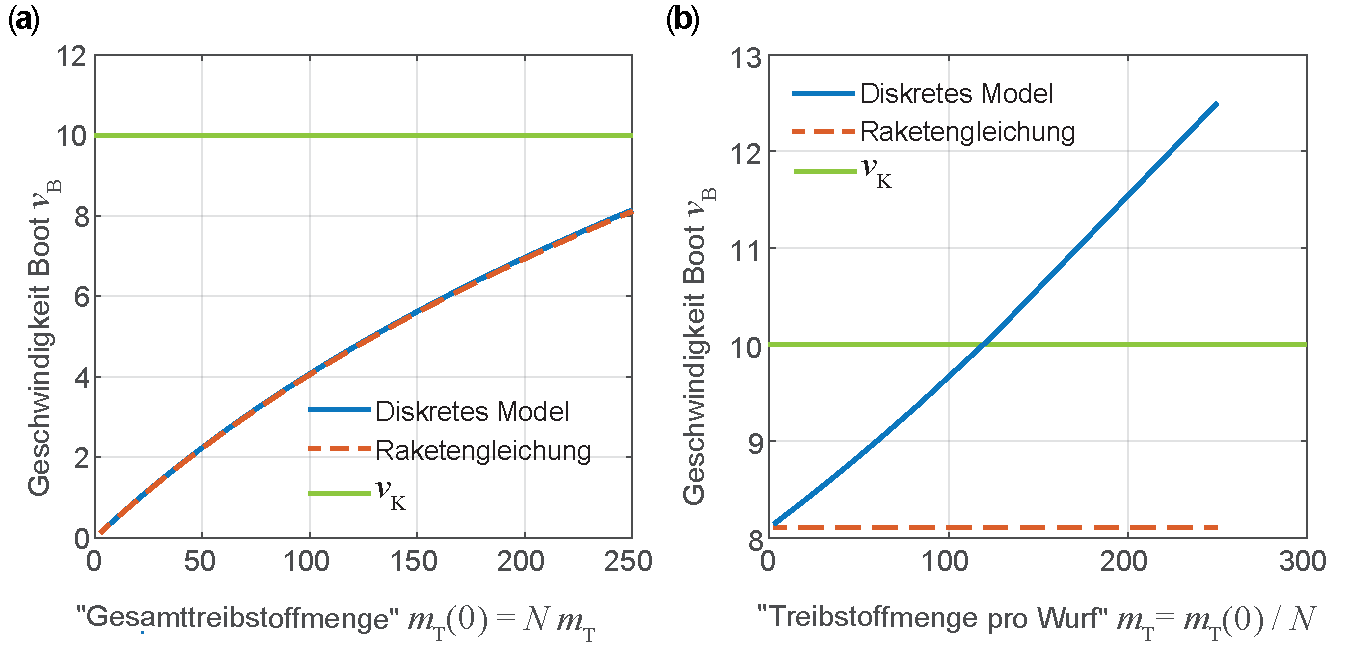
\includegraphics[width=\textwidth]{BoatRocketModelLsg.pdf}
\caption[Diskretes Modell der Raketengleichung.]{Diskretes Modell der Raketengleichung.}
\label{abb:adyn_RaketenAlternative}
\end{figure}


\begin{nebenrechnungNeu} {Grenzwertberechnung}
  
Wir wollen den Grenzwert bilden:
\begin{align}
    \lim_{N\to\infty} V_N &= v_\text{K} \lim_{N\to\infty} \lk \frac{1}{\mu-1} + \frac{1}{\mu-2} + \ldots + \frac{1}{\mu-n}\rk \nonumber \\
    &= v_\text{K} \lim_{N\to\infty} \lk \frac{x}{n-x} + \frac{x}{n-2x} + \ldots + \frac{n}{n-n\,x} \rk = S(x) \label{eq:adyn_RaketenAlt08}
\end{align}
Wir berechnen zun�chst die Partialsumme $S_k^n$, die die Summe aller Terme der Summe $V_n$ nach \eqref{eq:adyn_RaketenAlt08} bis zum $k$-ten Term beinhaltet. Wir definieren dies wie folgt rekursiv:
\begin{align}
    S_{k+1}^n = S_{k}^n + \frac{x}{n-\lk k+1\rk\,x} ~~~~ \text{mit} ~~~~ n=1,2,\ldots,N ~~~~\text{und} ~~~~ k = 0,1,\ldots,\lk n-1\rk\label{eq:adyn_RaketenAlt09}
\end{align}
Dabei ist:
\begin{align*}
    S_0^1 = 0
    \begin{cases}
        n=1,\, k=0
    \end{cases}
    ~~~\text{und}~~~
    S_1^1 = S_0^1 + \frac{x}{1-x} = \frac{x}{1-x}
    \begin{cases}
        n=1,\, k=1
    \end{cases}
\end{align*}
Wir bilden den Quotienten:
\begin{align}
    \frac{S_{k+1}^n - S_k^n}{x/n} = \frac{1}{1-\lk k+1\rk \,x/n}\label{eq:adyn_RaketenAlt10}
\end{align}
und bezeichnen der Einfachheit wegen: 
\begin{align}
    \lk k+1\rk\,\frac{x}{n} = \chi_\text{k} \label{eq:adyn_RaketenAlt11}
\end{align}
und 
\begin{align}
    S_{k+1}^n - S_k^n = \Delta S\lk \chi_\text{k}\rk\,.  \label{eq:adyn_RaketenAlt12}
\end{align}
Damit wird aus \eqref{eq:adyn_RaketenAlt10} der Differentialquotient
\begin{align}
    \frac{\Delta S\lk \chi_\text{k}\rk}{\Delta \chi_\text{k}} = \frac{1}{1-\chi_\text{k}}\,. \label{eq:adyn_RaketenAlt13}
\end{align}
Wir bilden den Grenzwert $n\to\infty$ und erhalten mit $S\lk \chi_\text{k}\rk$ das Riemann-Integral der rechten Seite:
\begin{align}
    S\lk \chi_\text{k}\rk = -\ln\lk 1-\chi_\text{k}\rk = \ln \lk \frac{1}{1-\chi_\text{k}}\rk\,. \label{eq:adyn_RaketenAlt14}
\end{align}
Mit \eqref{eq:adyn_RaketenAlt11} k�nnen wir f�r $n\to\infty$ auch schreiben ($k=n,\,\chi_\text{k}\to x$)
\begin{align*}
    S\lk \chi_\text{k}\rk = S\lk x\rk
\end{align*}
also:
\begin{align}
    \ln\lk \frac{1}{1-x}\rk = \lim_{n\to\infty} \lk \frac{x}{n-x} + \frac{x}{n-2x} +\ldots + \frac{x}{n-n\,x}\rk\,. \label{eq:adyn_RaketenAlt15}
\end{align}
Damit wird aus \eqref{eq:adyn_RaketenAlt11}
\begin{align}
    V= \lim_{n\to\infty} V_N = v_\text{k}\,\ln\lk\frac{1}{1-x}\rk = v_\text{k}\,\ln\lk\frac{1}{1-M_\text{T}/M_0}\rk = v_\text{k} \,\ln\frac{M_0}{M_0-M_\text{T}}\,, \label{eq:adyn_RaketenAlt16}
\end{align}
was genau der Raketengleichung \eqref{eq:adyn_rocketequ} entspricht. (Diese Rechnung wurde in �hnlicher Form zuerst in \cite{Lagos2023} gezeigt.)\\

\end{nebenrechnungNeu}


\end{sol} 
\textcolor{blue} {$\rightarrow$ zur} \probref{adyn_BoatRocketModel}.\\
\noindent\rule[1ex]{\textwidth}{0.5pt}  \newpage  \clearpage

%-----------------------------------------------------------------------------------------------------------
%-----------------------------------------------------------------------------------------------------------

\newpage
\subsection{Weiterf�hrende Zusatzaufgaben und Probleme}

\begin{sol}{prob:adyn_launchinnovations}\label{lsg:adyn_launchinnovations} %Zusatz1
\textbf{Neue Ideen zum Flug ins Weltall}\\

Wir zitieren aus der etwas sp�rlichen Information der Firma Spinlaunch (\url{www.spinlaunch.com}):
\begin{quotation}
\textit{The Suborbital Accelerator is designed to operate from 800 to 5,000 mph (approx. 8000 km/h) and acts primarily as a test-bed for the Orbital Launch System. On October 22nd, 2021, our first launch successfully propelled a test vehicle at supersonic speeds and ended with the recovery of the reusable flight vehicle. Throughout 2022 the system will conduct regular test flights with a variety of vehicles and launch velocities. The Suborbital System offers testing capabilities to customers and provides long term value as a satellite qualification facility.
}
\end{quotation}
So weit so gut. Schauen wir uns diese neueren Ideen f�r den Weltraumflug genauer an:\\
Den Weltraumfahrstuhl haben wir bereits in �bung 1.10 von Band I untersucht und verweisen daher auf die entsprechende L�sung.\\
Die \anf{Weltraumachterbahn}, wie der Spinlaunch auch genannt wird, ist ein neues Konzept und wir wollen uns die Machbarkeit unter drei Gesichtspunkten genauer anschauen. Wir benutzen dabei Angaben, die von der Fa. SpinLaunch \bzw in der Literatur im Internet zu finden sind.\\
Danach soll der Raumtransporter (Anfangsmasse von $m_0 = \SI{250}{\kg}$) die Zentrifuge mit einer Geschwindigkeit von $\SI{1000}{}$ - $\SI{8000}{\km\per\hour}$ verlassen und ohne Antrieb eine H�he von $\SI{60}{\km}$ �ber der Erdoberfl�che erreichen, wo eventuell noch einmal mit einer mitgenommenen Treibstoffmenge von $\SI{100}{\kg} \ldots \SI{150}{\kg}$
eine weitere Beschleunigung erfolgen kann. 
Der Durchmesser der Zentrifuge betr�gt etwa  $D=2R=\SI{50}{\metre}$.\\
Wir wollen untersuchen:
\begin{itemize}
    \item [1)] 
    \textbf{\textit{Mechanische Herausforderungen an die Zentrifuge}}:\\
    Es gilt: $v_0 = \omega\,D \quad \rightarrow \quad \omega = v_0/D$.\\
    Mit den geforderten Werten erhalten wir $\omega \approx 120,\ldots,1000\,\SI{}{\per\second}$.\\
    Wir gehen davon aus, dass das Raumschiff durch ein Gest�nge in der Zentrifuge geleitet wird. Das Gest�nge soll einen effektiven Durchmesser von $D = \SI{0.5}{\metre}$ haben und aus Stahl \bzw Kohlenfaserverbundstoffen bestehen.\\
    Die gesamte Zugspannung auf das Gest�nge  betr�gt dann:
    \begin{align*}
        \sigma = A\,\varrho\,\frac{R^2}{2}\,\omega^2 + m_0\,\omega^2\,\frac{R}{A} 
    \end{align*}
mit $A=\pi D^2/4$  und $\varrho \approx \SI{7e3}{\kg\per\cubic\metre}\,\text{(Stahl)}\, \text{\bzw}\, \varrho = \SI{2e3}{\kg\per\metre}\,\text{(Kohlenfaser)}$.  Wir erhalten\\
$\sigma = \SI{6.6}{\giga\Pa}$ (Stahl) \bzw $\sigma= \SI{2.2}{\giga\Pa}$ (Kohlenfaser).\\
Diese Werte sind dicht an der maximal erreichbaren Zugspannung vor einer m�glichen Zerst�rung. Hierin liegt also eine erste Herausforderung in der Lagerung des Zentrifugalarms, diese enormen Radialkraft muss ja durch das Lager aufgenommen werden.\\
    \item [2)]
    \textbf{\textit{Antriebsloser Aufstieg}}:\\
Nach Ausl�sen aus der Zentrifuge tritt der  Raumtransporter aus dem Vakuum in die Erdatmosph�re und erf�hrt auf dem Weg nach oben neben den gravitativen Verlusten auch Reibungsverluste.\\
    Wir k�nnen die Ergebnisse von \probref{adyn_launch01} benutzen und erhalten unter der Annahme von optimistischen Werten von $c_\text{w,R} = 0.2$ und $A_\text{R} = \pi\,\SI{0.25}{\square\metre}/4$ eine maximale H�he am Ende der Spin Launch Phase von $h_\text{end} = \SI{50}{\km},\ldots,\SI{60}{\km}$ \bzw eine Geschwindigkeit von $v_\text{end}\lk h=\SI{60}{\km}\rk\approx \SI{1.25}{\km\per\second}$.\\
    \item [3)]
    \textbf{\textit{Zusatzschub}}:\\
    Nimmt man an, dass bei $h=\SI{60}{km}$ noch $\SI{200}{\kg}$ Treibstoff mit $v_\text{G}=\SI{5000}{\metre\per\second}$ (sehr optimistisch) zur Verf�gung stehen, dann hat man dort f�r die verbleibende Nutzlast von $\SI{100}{kg}$ (ohne Strukturmasse) noch ein Geschwindigkeitsbudget von
    \begin{align*}
        \Delta v = v_\text{G}\,\ln\,\frac{m_\text{L}}{m_0}\, = \SI{5.9}{\km\per\second}
    \end{align*}
    zur Verf�gung, zus�tzlich der 
    \begin{align*}
        \Delta v_\text{E} \approx \SI{0.4}{\km\per\second}
    \end{align*}
    aus der Rotation der Erde.\\
    Gebraucht werden f�r eine Kreisbahn in $\SI{200}{\km}$:
    \begin{align*}
        v_\text{k} =  \sqrt{ \frac{\mu_\text{E}}{R_\text{E}}+\SI{200}{\km}}\approx \SI{7.85}{\km\per\second}\,,
    \end{align*}
    \dh unter den Annahmen kommt es zu keiner stabilen Kreisbahn in $\SI{200}{\km}$ H�he, es wird sich also um einen suborbitalen Flug handeln.\\
		\item [4)] 
    Wir wollen nun noch die energetischen Verh�ltnisse betrachten.\\
    Um eine Nutzlast von $\SI{100}{\kg}$ mit in eine H�he von $\SI{200}{\km}$ zu bringen, braucht man (ohne Ber�cksichtigung der Unterst�tzung durch die Erdrotation) ein Geschwindigkeitsbudget von 
    \begin{align*}
        \Delta v = \SI{7.85}{\km\per\second}
    \end{align*}
    \bzw bei Annahme einer Strukturmasse von $\SI{500}{\kg}$ eine Treibstoffmasse von 
    \begin{align*}
        m_\text{T} = m_\text{L} \, \lk \e^{+\frac{\Delta v}{v_\text{G}}} - 1 \rk - m_\text{S} \approx \SI{300}{\kg}\,.
    \end{align*}
    Man spart also in etwa $\SI{100}{\kg}$ Treibstoff. Daf�r muss man durch elektrischen Antrieb eine kinetische und Rotationsenergie von 
    \begin{align*}
        T = \frac{m_0}{2}\,v_0{}^2 + \frac{J}{2}\,\lk\frac{v_0}{R}\rk^2 = \frac{1}{2}\,v_0{}^2\,\lk m_0 + \frac{J}{R^2} \rk
    \end{align*}
    aufbringen, wenn $J$ das Tr�gheitsmoment des Rotationsarms ist.
    \begin{align*}
        J &= \frac{1}{3}\,m_{\text{Rotor}}\,R^2 = \frac{1}{3}\,\frac{\pi}{4}\,D^2\,R^3 \,\varrho \approx \SI{1.8}{\kg\square\metre}\\
        \rightarrow \quad T & \approx \SI{5.8}{\N\metre} \approx \SI{1.6}{\mega\watt\hour}
    \end{align*}
    Der \anf{eingesparte} Treibstoff (typische Parameter) hat einen \anf{Energieinhalt} von
    \begin{align*}
        E_{\text{chem}} &= \epsilon_\text{T}\,\Delta m_\text{T}\\
        &\approx \SI{3500}{\kilo\joule\per\mol}\cdot\SI{0.01}{\mol\per\g}\cdot\SI{100e3}{\g} \approx \SI{3.5e9}{\joule} \approx \SI{1}{\mega\watt\hour}
    \end{align*}
    Auch daran sieht man, dass man energetisch nicht wirklich etwas spart (wie k�nnte man auch?), jedoch w�re der Betrieb der SpinLaunch-Anlage nat�rlich mit \anf{nachhaltiger} Energie machbar.\\
    \item [5)]
    \textbf{\textit{Zusammenfassung}}:\\
    Alles in allem sieht das Projekt SpinLaunch etwas erfolgversprechender aus als der Erdfahrstuhl, wenngleich die ingenieurtechnischen Anforderungen riesig sind und auch der f�r 2022 angek�ndigte Erstflug bislang nicht erfolgt ist. \\
    In \figref{adyn_SpinLaunch} haben wir das Ergebnis der Simulation eines SpinLaunch-Unternehmens f�r eine Nutzlast von \SI{100}{\kg} und einem \textit{on-board} Treibstoffvorrat von $\SI{200}{\kg}$ dargestellt. Auch sonst sind alle anderen Annahmen extrem optimistisch gemacht. Man erkennt, dass dieses Prinzip bestenfalls f�r kleinere Nutzlasten machbar/sinnvoll erscheint, wobei wir mal von den \anf{kleinen} ingenieurtechnischen Herausforderungen wie Vakuum f�r die Zentrifuge, Stabilit�t der Materialien, Bewegung von $\SI{200}{\kg}$ Treibstoff bei einer \anf{leicht erh�hten} Zentrifugalbeschleunigung von $a_\text{z} = v_0{}^2/R\approx \SI{20e3}{} g$ absieht.
\end{itemize}


\begin{figure}
	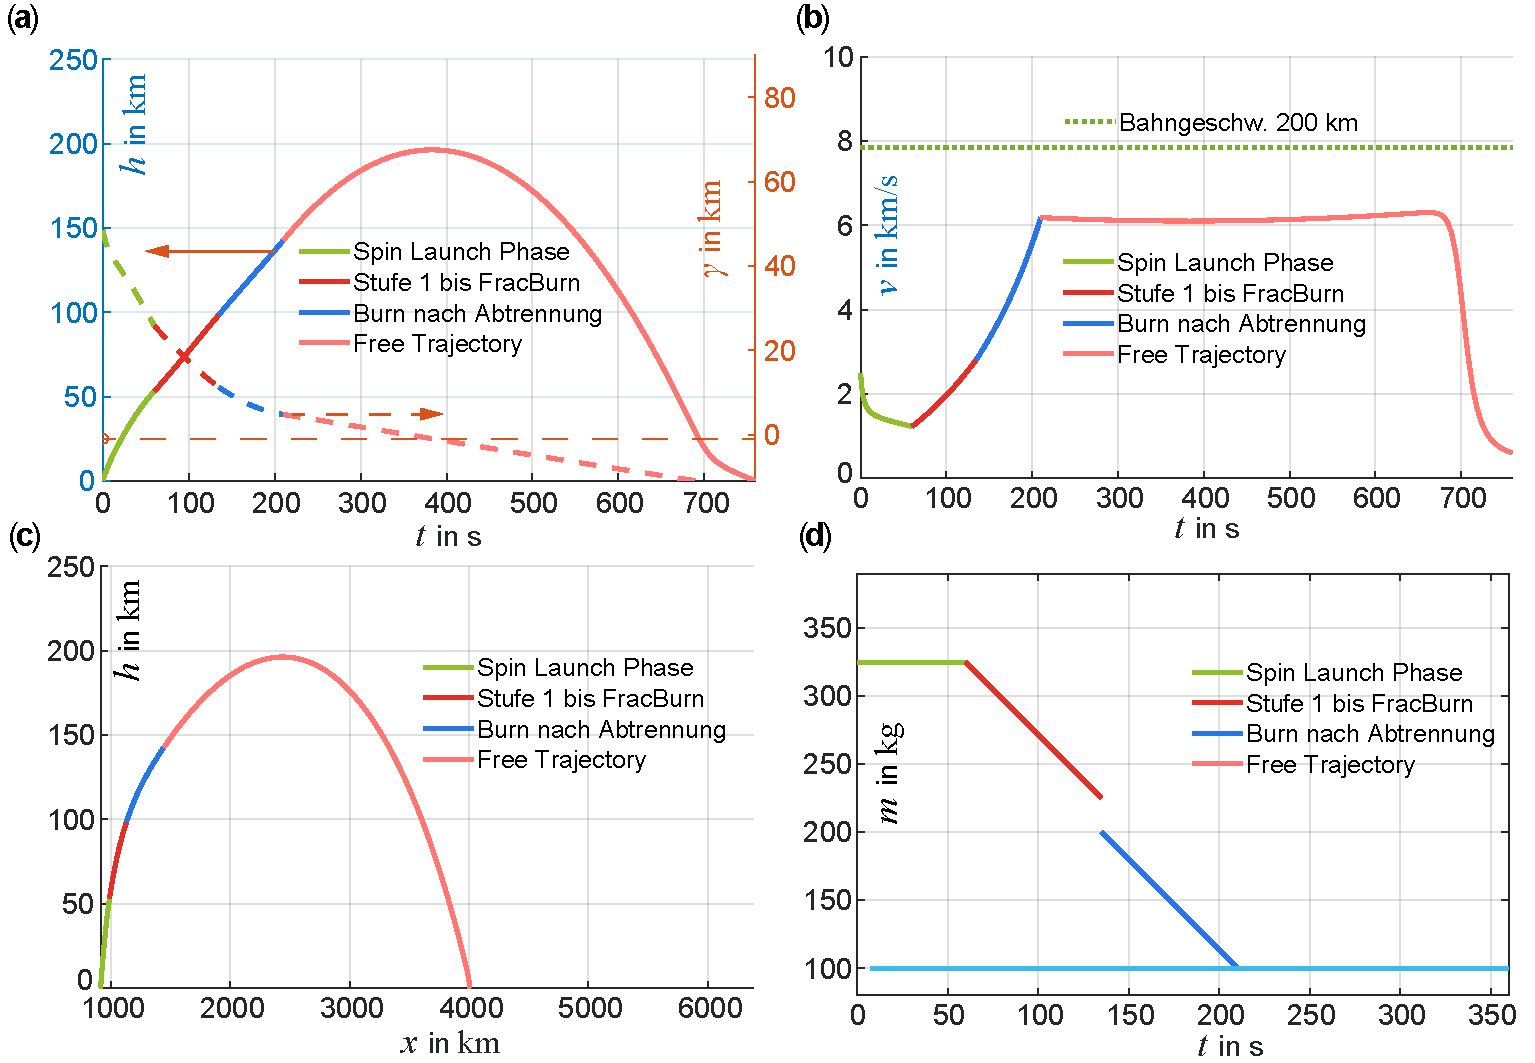
\includegraphics[width=\textwidth]{Spinlaunch.pdf} 
	\caption[Beispielrechnungen zum Spinlaunch.]{Beispielrechnungen zum Spinlaunch. Parameter siehe Text und \mscr~\mladynref{Spinlaunch.m} \fa H�he und FPA �ber die Zeit \fb Geschwindigkeit �ber die Zeit \fc H�he �ber Horizontkoordinate $x$ \fd Masse des Raumtransporters �ber die Zeit.}
	\label{abb:adyn_SpinLaunch}
\end{figure}

\end{sol} 
\textcolor{blue} {$\rightarrow$ zur} \probref{adyn_launchinnovations}.\\
\noindent\rule[1ex]{\textwidth}{0.5pt} \newpage  \clearpage


%-----------------------------------------------------------------------------------------------------------

\begin{sol}{prob:adyn_orbits_zusatz2}\label{lsg:adyn_orbits_zusatz1} %Zusatz
\textbf{Bahnparameter aus Bodenbeobachtungen (Ortsvektoren)}\\

Zun�chst m�ssen wir aus den topozentrischen Messwerten ($\vec{R}$ mit Distanz $R$, Azimut $\mathcal{A}$ und H�he $h$) geozentrisch-�quatoriale Messwerte "`machen"'. Wir invertieren dazu \eqref{eq:adyn_statobserv06} und erhalten:
\begin{align}
	  \vec{r} =  \mathbb{R}_\text{z}\lk -\theta\rk \, \lek \mathbb{U}^{-1} \,\vec{R} + \vec{r}_\text{B} \rek \,, \label{eq:adyn_bahnbest_lsg01}
\end{align}
worin $\vec{r},\, \vec{r}_\text{B}$ die geozentrische-�quatorialen Koordinatenvektoren f�r Satellit und Beobachtungsstation sind und  $\vec{R}$ die topozentrischen Koordinaten des Satelliten.\\
Mit den so bestimmten Vektoren $\vec{r}_1$ und $\vec{r}_2$ zu den beiden Messzeiten /$t_1,$ und $t_2$ kann man nach einer von Gau� entwickelten geometrisch-iterativen Methode die Bahnparameter bestimmen. Im folgenden ist diese der Darstellung in \cite{Montenbruck2012} folgend skizziert. Wir starten mit \figref{adyn_orbit_determination} und gehen wie folgt vor:

\begin{figure}
	\includegraphics[width=\textwidth]{BestimmungOrbitsGauss.pdf} 
	\caption[Bestimmung von Bahnparametern von Satelliten.]{Zur Bestimmung von Bahnparametern von Satelliten aus Orts- und Winkelbeobachtungen.}
	\label{abb:adyn_orbit_determination}
\end{figure}

\begin{enumerate}
    %1
    \item Man benutzt, dass die Bahnebene eines Satelliten immer durch die Ebene gegeben ist, die durch die beiden Vektoren $\vec{r}_1$, $\vec{r}_2$ aufgespannt wird. \\
    Man bestimmt dann �ber die Einheitsvektoren 
    \begin{align}
        \vec{e}_1 &= \frac{\vec{r}_1}{|\vec{r}_1|}~~~~ \text{und} ~~~~ \vec{e}_0 = \frac{\vec{r}_0}{|\vec{r}_0|} \label{eq:adyn_bahnbest_15}
    \end{align}
    mit $\vec{r}_0 = \vec{r}_2 - \lk \vec{r}_2\,\vec{e}_1\rk\,\vec{e}_1$ und den Gau�-Vektor \\
   \begin{align}
			\vec{W} &= \vec{L}/|\vec{L}| = \vec{e}_1\times \vec{e}_0 =\begin{pmatrix} W_x\\W_y\\W_z \end{pmatrix} \,, \label{eq:adyn_bahnbest_15a}
	\end{align}
		der senkrecht auf der Bahnebene steht.\\
    %2
    \item Wir erhalten damit sofort die Inklination 
    \begin{align}
        i = \arctan \lk\frac{\sqrt{W_x{}^2+W_y{}^2}}{W_z}\rk \label{eq:adyn_bahnbest_16}
    \end{align}
    und die Rektaszension des aufsteigenden Knotens 
    \begin{align}
        \Omega = \arctan \lk\frac{W_x}{-W_y}\rk \,. \label{eq:adyn_bahnbest_17}
    \end{align}
    Ebenso bestimmt man das Argument der L�nge, welches wir sp�ter noch ben�tigen: 
    \begin{align}
        u_1 =\arctan\lk\frac{z_1}{-x_1\,W_y +y_1\,W_x}\rk\,. \label{eq:adyn_bahnbest_17a}
    \end{align}
    %3
    \item Zur Bestimmung der restlichen Bahnparameter braucht man einige Hilfsgr��en, wir verweisen f�r eine detailliertere Darstellung auf die Literatur \cite{Montenbruck2012, Bucerius1950, Escobal1965}. \\
		
		Mit dem Bahnparameter $p$ der Ellipse $p=a\,(1-e^2) $ findet man die Sektorenfl�che nach dem 2. Keplerschen Gesetz (\figref{adyn_orbit_determination}a zu:
    \begin{align}
        A_\text{S} = \frac{1}{2} \sqrt{G\,m_\text{E}}\,a\,(1-e^2)\,\lk t_2 -t_1\rk  \,. \label{eq:adyn_bahnbest_19a}
    \end{align}
		Die entsprechende durch $\vec{r}_1$ und $\vec{r}_2$ definierte Dreiecksfl�che nach \figref{adyn_orbit_determination}b ist:
		    \begin{align}
        A_\Delta = \frac{1}{2}\,r_1\,r_2\,\sin\lk \upsilon_2-\upsilon_1\rk= \frac{1}{2}\,r_1\,r_0 \,.\label{eq:adyn_bahnbest_19b}
    \end{align}
		Ferner setzen wir 
    \begin{align}
        \tau = \sqrt{G\,m_\text{E}}\,\lk t_2 -t_1\rk  \label{eq:adyn_bahnbest_20a}
    \end{align}
		 als eine mit $\sqrt{G\,m_\text{E}}$ multiplizierte Zeit zwischen den zwei Messungen. Wir definieren nun die Gr��e  $\eta$ als das  Verh�ltnis von Sektorfl�che $A_\text{S}$ zu Dreiecksfl�che $A_\Delta$ und erhalten:
    \begin{align}
        \eta = \frac{A_\text{S}}{A_\Delta} = \frac{\sqrt{p}\,\tau}{r_1\,r_2\,\sin(\upsilon_2 - \upsilon_1)} \label{eq:adyn_bahnbest_20b}
    \end{align}
		Hat man $\eta$ berechnet, kann man �ber   
    \begin{align}
        p = \lk \frac{2\,A_\Delta\,\eta}{\tau} \rk^2\,, \label{eq:adyn_bahnbest_18}
    \end{align}
    den Parameter $p$ der Bahnellipse bestimmen. Dieser, wie auch die wahren Anomalien, sind aber noch unbekannt, ebenso wie $\eta$. Ersetzt man diese durch die Gr��en aus der Bahngleichung \bzw Kepler-Gleichung, wobei man mit $\zeta = \lk E(t_2) - E(t_1) \rk /2 $ eine Hilfsgr��e einf�hrt, erh�lt man f�r $\eta$ und $\zeta$ das folgende nichtlineare Gleichungssystem 
    \begin{align}
    \begin{split}
        \eta^2\,\lk \eta-1\rk &= m\,\frac{2\zeta -\sin\lk 2\zeta\rk}{\sin^3\lk\zeta\rk}\,, \\
        \eta^2 &= m\,\frac{1}{k+\sin^2\lk \zeta/2 \rk}
    \end{split} \label{eq:adyn_bahnbest_21}
    \end{align}
		mit den Abk�rzungen f�r die Kombination der bekannten Gr��en $\vec{r}_1, \vec{r}_2$:
    \begin{subequations}
    \begin{align}
        m &= \frac{\tau^2}{\sqrt{2\,\lk r_1\,r_2 + \vec{r}_1\,\vec{r}_2\rk}^3}  ~~~\text{und} \label{eq:adyn_bahnbest_22a}\,, \\
        k &= \frac{r_1+r_2}{2\sqrt{2\,\lk r_1\,r_2 + \vec{r}_1\,\vec{r}_2\rk}}-\frac{1}{2}\,. \label{eq:adyn_bahnbest_22b}
    \end{align}
    \end{subequations}
		Die L�sung des nichtlinearen Gleichungssystems \eqref{eq:adyn_bahnbest_21} ergibt sowohl $\eta$ als auch $\zeta$, wobei man eigentlich nur $\eta$  f�r die weitere Berechnung braucht.\\
    %4
    \item Die numerische L�sung f�r $\eta$ findet man mit \matlab �ber drei Wege:		
		\begin{enumerate}
			\item [a)] Man l�st das nichtlinearen Gleichungssystems \eqref{eq:adyn_bahnbest_21} mit Hilfe des \matlab-Solvers \textcolor{mygreen}{\texttt{fsolve}}. Hierzu 
			muss eine Vektorfunktion $\vec{F}_2 = \mathrm{func2d}(\vec{x})$ der Vektorvariablen $\vec{x} = [x(1), x(2)] = [\eta, \zeta]$ definiert werden.
			\item [b)] Man eliminiert aus dem nichtlinearen Gleichungssystems \eqref{eq:adyn_bahnbest_21} die Variable $\zeta$ und erh�lt die Funktion 
			 \begin{align}
				  F_1 &= \mathrm{func1d}(\eta) = 1 - \eta + \frac{m}{\eta^2}\,\frac{2q(\eta)-\sin\lk 2q(\eta) \rk}{\sin\lk q(\eta) \rk^3}~~~\text{mit}~~\label{eq:adyn_bahnbest_23a}\\
					~q &= 2\asin\lk \frac{m}{\eta^2} - k \rk \,, \nonumber 
			 \end{align}
			deren Nullstelle man mit Hilfe des \matlab-Solvers \textcolor{mygreen}{\texttt{fzero}} sucht. 
			\item [c)q] Man startet mit \eqref{eq:adyn_bahnbest_23a} und bestimmt die Nullstelle durch eine Iteration nach folgendem Iterationsschema \cite{Montenbruck2012}:
    \begin{align}
        \eta_{i+1} = \eta_i -f\lk\eta_i\rk\,\frac{\eta_i -\eta_{i-1}}{f\lk \eta_i\rk - f\lk\eta_{i-1}\rk} \label{eq:adyn_bahnbest_23b}
    \end{align}
    mit 
    \begin{subequations}
    \begin{align}
        f\lk\eta_i\rk &= 1-\eta_i + \frac{m}{\eta_i{}^2}\,\lek \frac{4}{3} + \frac{4\cdot 6}{3\cdot 5}\,\lk\frac{m}{\eta_i{}^2}-k\rk + \frac{4\cdot 6\cdot 8}{3\cdot 5\cdot 7}\,\lk\frac{m}{\eta_i{}^2}-k\rk^2 +\ldots\rek\label{eq:adyn_bahnbest_24a}
    \intertext{und den Anfangswerten}
        \eta_0 &= \frac{12}{22} + \frac{10}{22}\,\sqrt{1+\frac{44}{9}\,\frac{m}{k+\frac{5}{6}}} \label{eq:adyn_bahnbest_24b}\\
        \eta_1 &= \eta_0 + 0.1  \label{eq:adyn_bahnbest_24c}
	 \end{align}
    \end{subequations}
		\end{enumerate}
    %5
    \item  Hat man nach einer der drei Methoden $\eta$ berechnet, kann man �ber \eqref{eq:adyn_bahnbest_18} den Ellipsen-Parameter $p$ bestimmen und �ber die Ellipsengleichung 
		\begin{align*}
        e\,\cos\lk\upsilon_1\rk = \frac{p}{r_1}-1\,,~~~ e\,\cos\lk\upsilon_2\rk = \frac{p}{r_2}-1
    \end{align*}
    folgende Bestimmungsgleichungen f�r $\upsilon_1$ und $e$ erhalten:
    \begin{subequations}
    \begin{align}
        e\,\cos\lk\upsilon_1\rk &= \frac{p}{r_1}-1 \label{eq:adyn_bahnbest_25a}\,,\\
        e\,\sin\lk\upsilon_1\rk &= \frac{\lk \frac{p}{r_1}-1\rk\,\lk \frac{\vec{r}_2\,\vec{e}_1}{r_2}\rk-\lk\frac{p}{r_2}-1\rk}{\frac{r_0}{r_2}} \,,\label{eq:adyn_bahnbest_25b}
    \end{align}
    \end{subequations}
    woraus folgt:
    \begin{align}
        \upsilon_1 = \arctan{\lek \frac{\lk \frac{p}{r_1}-1 \rk \, \lk \frac{\vec{r}_2\,\vec{e}_1}{r_2}\rk-\lk\frac{p}{r_2}-1\rk}{\frac{r_0}{r_2}\,\lk\frac{p}{r_1}-1\rk} \rek}
				\label{eq:adyn_bahnbest_26a}
    \end{align}
    \bzw
    \begin{align}
        e = \sqrt{\lk \frac{p}{r_1}-1 \rk^2 + \frac{\lk \lk \frac{p}{r_1}-1\rk\,\lk \frac{\vec{r}_2\,\vec{e}_1}{r_2}\rk-\lk\frac{p}{r_2}-1\rk\rk^2}{\lk \frac{r_0}{r_2}\rk^2}} \,.\label{eq:adyn_bahnbest_26b}
    \end{align}
		%6
    \item Das Argument des Perig�ums $\omega$ bestimmt man �ber 
    \begin{align}
        \omega = u_1 -\upsilon_1 ~~~\text{mit dem Argument der L�nge}~~u_1 = \arctan \lk \frac{z_1}{-x_1\,W_y + y_1\,W_x} \rk \label{eq:adyn_bahnbest_26c}
    \end{align}
    und die gro�e Halbachse $a$ �ber
    \begin{align}
        a = \frac{p}{1-e^2}\,.  \label{eq:adyn_bahnbest_26d}
    \end{align}
    %7
    \item Als sechstes und letztes Bahnelement berechnet sich die mittlere Anomalie zum Zeitpunkt $t_1$ �ber die Kepler-Gleichung 
    \begin{align}
        M_1= E_1 -e\,\sin E_1 \label{eq:adyn_bahnbest_26e}
    \end{align}
    mit der exzentrischen Anomalie 
    \begin{align}
        E_1 = \arctan \lk\frac{\sqrt{1-e^2}\,\sin\upsilon_1}{\cos\upsilon_1 +e}\rk\,. \label{eq:adyn_bahnbest_26f}
    \end{align}
\end{enumerate} 

Die Rechnungen sind im Detail im \mscr~\mladynref{BahnparaBestimmung02.m} hinterlegt.\\

\textbf{Hinweis:} Man muss bei der Bestimmung der Bahnparameter etwas aufpassen, ob die Beobachtungszeiten zum gleichen Umlauf geh�ren oder ob der Satellit inzwischen nicht bereits eine oder mehrere Erdumrundungen vollzogen hat. Im angegebenen Beispiel relativ kurzer Zeiten zwischen zwei Beobachtungen ist sicher davon auszugehen, dass die Daten zum gleichen Umlauf geh�ren.\\

\textbf{Zusatzaufgabe:} In \kap{adyn_lambert_transfer} bzw \probref{adyn_manoevers4} haben wir bei der Behandlung des Lambert-Problems noch eine andere Methode kennen gelernt, wie das Problem der Bestimmung der Bahnparameter  gel�st werden kann. Hierzu bestimmt man aus den gemessenen $\vec{r}_1$ und $\vec{r}_2$ den Winkel $\gamma$ und nimmt als Flugzeit (TOF) des Satelliten auf seine Bahn die Differenz der Beobachtungszeiten. Wir empfehlen zur Vertiefung auch diese Aufgabe hier mit der Methode des Lambert-Transfers zu l�sen.

\end{sol} 
\textcolor{blue} {$\rightarrow$ zur} \probref{adyn_orbits_zusatz2}.\\
\noindent\rule[1ex]{\textwidth}{0.5pt}  \newpage  \clearpage
%
%%-----------------------------------------------------------------------------------------------------------------------------------------------


\begin{sol}{prob:adyn_orbits_zusatz2}\label{lsg:adyn_orbits_zusatz2} %Zusatz
\textbf{Bahnparameter aus Bodenbeobachtungen (Ortsvektoren)}\\

Wir verweisen auf das \mscr~ \mladynref{BahnparaBestimmung03.m}.

\end{sol} 
\textcolor{blue} {$\rightarrow$ zur} \probref{adyn_orbits_zusatz2}.\\
\noindent\rule[1ex]{\textwidth}{0.5pt} \newpage  \clearpage

%-----------------------------------------------------------------------------------------------------------------------------------------------

\begin{sol}{prob:adyn_swingby02}\label{lsg:adyn_swingby02} %Zusatz
\textbf{Gravity-Assist-Man�ver - Allgemeiner Fall}\\

\begin{figure}
	\includegraphics[width=\textwidth]{GeschwindigkeitenSOI.pdf} 
	\caption[Geometrie und Geschwindigkeiten beim Gravity-Assist-Man�ver am Punkt $\mathrm{P}_1$.]{Geometrie und Geschwindigkeiten beim Gravity-Assist-Man�ver am Punkt $\mathrm{P}_1$. Bahnebene des Swing-By und Planetenbahnebene fallen hier gem�� Annahme noch zusammen. }
	\label{abb:adyn_swby01}
\end{figure}

\begin{enumerate}
    %1
    \item [1)]
		Wir definieren zun�chst die Vektoren im Inertialsystem (\figref{adyn_swingby01} und \figref{adyn_swby01}):
    \begin{align*}
        \vec{r}_\text{P} \quad &\text{Vektor zum Planeten} \\
        \vec{r}_\text{R} \quad &\text{Vektor zum Raumschiff} \\
        \vec{v}_1 \quad &\text{Geschwindigkeit des Raumschiffs beim Eintreffen an der SOI des Planeten}\\
        \vec{v}_\text{P} \quad &\text{Geschwindigkeit des Planeten}
    \end{align*} 
    %2
    \item [2)]
    Wir definieren die Geschwindigkeit und den Abstand zum Planeten beim Eintreffen an der SOI im planetozentrischen \KOS:
    \begin{align}
    \begin{split}
        \vec{r}_1{}' &= \vec{r}_\text{R} - \vec{r}_\text{P}\,, \\
        \vec{v}_1{}' &= \vec{v}_1 - \vec{v}_\text{P}\,, \\
              v_1{}' &= |\vec{v}_1{}'| = v_\infty\,, \\
    \end{split} \label{eq:adyn_swby01}
    \end{align}
    Wir wollen dabei zun�chst gem�� \figref{adyn_swby01} noch die Vereinfachung machen, dass die Orbitalebene des Planeten mit der Swing-By Ebene zusammenf�llt, wir werden sp�ter weiter unten diese Einschr�nkung fallen lassen (siehe dazu auch \figref{adyn_GA3dim}).
    %3
    \item [3)]
    Den vektoriellen Sto�parameter $\vec{b}$ k�nnen wir dann ebenfalls definieren, er ergibt sich nach einfachen geometrischen �berlegungen aus \figref{adyn_swby01} zu
     \begin{align}
     \begin{split}
         \vec{b} & =\vec{r}_1{}' + \frac{\vec{v}_1{}'}{v_1{}'^2}\,\lk -\vec{r}_1{}'\cdot\vec{v}_1{}' \rk = \vec{r}_1{}' - \frac{\vec{v}_1{}'}{v_1{}'^2}\,\lk \vec{r}_1{}'\cdot\vec{v}_1{}' \rk \,.
     \end{split}
     \label{eq:adyn_swby02}
     \end{align}
		
\begin{figure}
	\includegraphics[width=\textwidth]{SwingByHyperbel.pdf} 
	\caption[Ablenkwinkel beim Gravity-Assist-Man�ver.]{Ablenkwinkel beim Gravity-Assist-Man�ver.}
	\label{abb:adyn_swby02}
\end{figure}
%
 Mit \eqref{eq:adyn_swby02} kann man mathematisch sauber zwischen einem Swing-By vor \bzw hinter dem Planeten unterscheiden (\vgl \figref{adyn_swingby00}):
     \begin{align*}
         \text{vor Planeten:} \quad &\vec{b}\,\vec{v}_\text{P} > 0 \\
         \text{hinter Planeten:} \quad &\vec{b}\,\vec{v}_\text{P} < 0
     \end{align*}
Wir wissen, aus \kap{adyn_gravity_assist} und insbesondere \figref{adyn_swingby00}, dass der Ablenkwinkel vorzeichenabh�ngig ist. Wir wollen diese Abh�ngigkeit nun dem Sto�parameter zuordnen und k�nnen aus \figref{adyn_swby02} und mit den Kenntnissen zur Geometrie der Hyperbel ablesen:
     \begin{align*}
         \tan \varphi' &= \tan(180\degree -\theta_\infty) = -\tan \theta_\infty = \frac{b}{-a} ~~~\text{mit}~~~
				 a = -\frac{\mu_\text{P}}{v_\infty{}^2}
     \end{align*}
Aus $\vartheta'/2 = \pi/2 - \varphi'$ folgt dann:
     \begin{align}
        \tan\lk\frac{\vartheta'}{2}\rk = \tan\,\lk \pi/2 - \varphi'\rk  =  \frac{1}{\tan\varphi'} = \frac{-a}{b} = \frac{\mu_\text{P}}{b\,v_\infty{}^2}\,.\label{eq:adyn_swby06}
     \end{align}
Offensichtlich ist $\vartheta'$ abh�ngig vom Vorzeichen von $b$.\footnote{Der Betrag des Ablenkungswinkels $\vartheta'$ ist nat�rlich identisch mit dem in Gleichung \eqref{eq:adyn_Streuung13b} hergeleiteten Winkel nach\\ $\sin\lk |\vartheta|/2 \rk = 1/ \lek 1 + \lk v_\infty{}^2\,r_{\text{Per}}/\mu_\text{P} \rk \rek\,$.}
Wir bestimmen nun das Vorzeichen von $\vartheta'$ �ber
    \begin{align}
         \sgn\lk\vartheta'\rk &= \sgn\lek \lk\vec{r}_\infty\times \vec{b}\rk\,\vec{e}_n\rek = \sgn\lek \lk\vec{r}_\infty\times \vec{b}\rk_z \rek] = \sgn\lk r_{\text{in},x}\,b_y - r_{\text{in},y}\,b_x\rk\,.\label{eq:adyn_swby04}
     \end{align}
Hierin ist $\vec{e}_n = \vec{e}_z$ der Normalenvektor der Bahnebene ist, der parallel zum Drehimpuls liegt und in die $z$-Richtung zeigt, w�hrend die Koordinaten $x, y$ in der Ebene des Swing-By-Orbits liegen.\footnote{Wir weisen darauf hin, dass die SOI nach dem ZKP-Prinzip eine \anf{eigene} Bahnebene definiert, die von der Anfangsbahnebene verschieden sein kann.}\\ 

Mit \eqref{eq:adyn_swby04} k�nnen wir f�r den mit einem Vorzeichen behafteten Wert des Sto�parameters schreiben:
     \begin{align}
         b = \sgn\lk\vartheta\rk \, |\vec{b}| = \sgn\lk r_{\text{in},x}\,b_y - r_{\text{in},y}\,b_x\rk\,|\vec{b}|\,.\label{eq:adyn_swby05}
     \end{align}
     %5
     \item [4)]
     Wir m�ssen jetzt noch die \anf{Drehung} des Swing-By mathematisch beschreiben, was sich am einfachsten mit Rotationsmatritzen machen l�sst.
     Dabei m�ssen wir zun�chst die Geschwindigkeit $\vec{v}_1$ in das planetozentrische System transformieren (wir erhalten $\vec{v}_1{}'$). \\
     Dann drehen wir $\vec{v}_1{}'$ um den Winkel $\vartheta'$ und erhalten $\vec{v}_2{}'$ im planetozentrischen System, welchen wir am Schluss wieder ins heliozentrische System zur�ck transformieren, um $\vec{v}_2$ zu erhalten. Dabei haben wir zun�chst weiterhin angenommen, dass der Swing-By in der Bahnebene des Planeten stattfindet. Wir k�nnen also schreiben:
     \begin{align}
         \vec{v}_2 = \mathbb{R}_\vartheta\,\lk\vec{v}_1 - \vec{v}_\text{P}\rk + \vec{v}_\text{P} \quad \text{mit} \quad \mathbb{R}_\vartheta = \begin{pmatrix}
             \cos\vartheta' & -\sin\vartheta' \\
             \sin \vartheta' & \cos\vartheta'
         \end{pmatrix}\,. \label{eq:adyn_swby07}
     \end{align}
     Unter Benutzung von trigonometrischen Formeln f�r den $\sin$, $\cos$ und $\tan$ erhalten wir schlie�lich: 
    \begin{align}
    \begin{split}
        \mathbb{R}_\vartheta &= 
        \begin{pmatrix}
            \cos\vartheta & -\sin\vartheta & 0 \\
            \sin \vartheta & \cos\vartheta & 0 \\
            0 &0&1
        \end{pmatrix}\\
        &= \frac{1}{1+\alpha^2}
        \begin{pmatrix}
            \alpha^2-1 & -2\alpha & 0\\
            2\alpha & \alpha^2-1 & 0 \\
            0 & 0 & 1+\alpha^2
        \end{pmatrix} 
        \quad \text{mit} \quad \tan\frac{\vartheta}{2} = \frac{1}{\alpha} = \frac{v_\text{P}{}^2}{b_n\,v_\infty{}^2}
    \end{split}\,. \label{eq:adyn_swby08}
    \end{align}
  Hierbei haben wir die Rotationsmatrix auf den dreidimensionalen Fall erweitert.\\
	\item [6)]
   Die Matrix in \eqref{eq:adyn_swby08} zusammen mit \eqref{eq:adyn_swby07} gelten nach unseren Einschr�nkungen nur f�r den Fall, dass die Bahnebene im planetozentrischen System, das durch die Vektoren $\vec{v}_1{}'$ und $\vec{b}$ aufgespannt wird, mit der Orbitalebene des Gravity-Assist-Planeten zusammen f�llt.\\
    Im allgemeinen Fall, in welchem diese beiden Bahnebenen nicht notwendigerweise �bereinstimmen (\figref{adyn_GA3dim}), muss man zun�chst die Vektoren aus dem heliozentrischen System in das Swing-By-\KOS (aufgespannt durch $\vec{v}_1{}'$, $\vec{b}$ und $\vec{L}$) transformieren. Das sind zwei Rotationen mit Eulerwinkeln (siehe Kap. 1.4.2.2 in Band I) und zwar zun�chst um die $z$-Achse um den Winkel $\varphi_{\text{Euler}}$ und dann um die neue $x$-Achse um den Winkel $\vartheta_{\text{Euler}}$. \\
    Wir wollen diese Rotationsmatrix mit $\mathbb{U}_\text{Euler}$ bezeichnen. Der Vektor der Geschwindigkeit $\vec{v}_2$ im heliozentrischen System ergibt sich dann zu:
    \begin{align}
          \vec{v}_2 = \mathbb{U}^\intercal_{\text{Euler}}\,\mathbb{R}_\vartheta\,\mathbb{U}_{\text{Euler}} \,\lk \vec{v}_1 - \vec{v}_\text{P}\rk + \vec{v}_\text{P}\,.  \label{eq:adyn_swby09}
    \end{align}
    Wir empfehlen als Zusatzaufgabe, die Matrix $\mathbb{U}_\text{Euler}$ selbst zu berechnen. 
\end{enumerate}

\end{sol} 
\textcolor{blue} {$\rightarrow$ zur} \probref{adyn_swingby02}.\\
\noindent\rule[1ex]{\textwidth}{0.5pt} \newpage  \clearpage


%---------------------------------------------------------------------------------------------------


\begin{sol}{prob:adyn_swingby04}\label{lsg:adyn_swingby04} %Zusatz
\textbf{Gravity-Assist-Man�ver - Zus�tzlicher Schub}\\

Wir wollen annehmen, dass das Raumschiff beim Perizentrumsdurchgang einen zus�tzlichen Schub mit einem Geschwindigkeitsbudget  $\Delta v_\text{per}$ bekommt und zwar tangential, \dh mit $\text{FPA} = 0$. Dies ist eine Anwendung des Oberth-Effktes\index{Oberth-Effekt} (siehe \kap{adyn_maneuvers} und \probref{adyn_rocket_analogy}).\\Wir wollen mit Gleichung \eqref{eq:adyn_lsgswingby02b} starten. 
In dieser wird $v_2$ maximal, wenn $\beta_2' = 0$ ist, was wir der Einfachheit halber annehmen wollen. Der periplanetare Abstand (Abstand Planet zum Perizentrum \bzw kleinster Bahnabstand zum Planeten) ist gegeben durch:
\begin{align}
     r_{\text{per}} = \frac{L^2}{\mu_\text{P}\,(e+1)} = -a\,(e-1) = \frac{\mu_\text{P}}{v_{\infty}{}^2}\,\lk \e - 1\rk\,. \label{eq:adyn_swby_oberth01}
\end{align}
Man kann nat�rlich auch die Geschwindigkeit am Perizentrum bestimmen:
\begin{align}
    v_{\text{per}} = \frac{\mu_\text{P}}{L} (e+1) = \sqrt {- \frac{\mu_\text{P}}{a}}\,\sqrt{\frac{e+1}{e-1}} \,. \label{eq:adyn_swby_oberth02}
\end{align}
Beide Gr��en seien durch $v_1$ bekannt, wir geben dieses, das $\Delta v$ und den Abstand $r_{\text{per}}$ vor, dann k�nnen wir $v_{\text{per}}$ und $v_2'$ berechnen und auch die Geschwindigkeit $\vec{v}_{2,\Delta\text{v}}$ beim Verlassen der SOI am Punkt $P_2$ (\figref{adyn_swingby01}). \\
Wie man erwarten kann, wird $\vec{v}_{2,\Delta\text{v}}$ \bzw $\vec{v}_{2,\Delta\text{v}}'$ und auch die Bahnform nach dem Perizentrums-Durchgang von $\vec{v}_2$ \bzw $\vec{v}_2{}'$ ohne $\Delta v$ abweichen.\\
Wir k�nnen uns leicht �berlegen, dass das Raumschiff bis zum Burn am Perizentrum auf einer Hyperbel mit den Parametern $a, e$ fliegt und nach dem Burn auf einer Hyperbel mit den Parametern $\hat{a}, \hat{e}$. Es gilt dann:
\begin{subequations}
\begin{align}
    \frac{v_\text{per}{}^2}{2}- \frac{\mu_\text{P}}{r_\text{per}} & =  \frac{v_1{}'^2}{2}\,, \label{eq:adyn_swby_oberth03a} \\
    \frac{\lk v_\text{per} +\Delta v \rk ^2}{2}- \frac{\mu_\text{P}}{r_\text{per}} & =  \frac{v_2{}'^2}{2} \,. \label{eq:adyn_swby_oberth03b}
\end{align}
\end{subequations}

Die Hyperbel nach dem Durchgang durchs Perizentrum hat dann folgende Parameter:
\begin{subequations}
\begin{align}
     \hat{a} &= - \frac{\mu_\text{P}}{v_2{}'^2}\,,\label{eq:adyn_swby_oberth04a} \\
		 \hat{e} & =  \frac{\lk v_\text{per} +\Delta v \rk ^2\,r_\text{per}}{\mu_\text{P}} - 1 \,. \label{eq:adyn_swby_oberth04b}
\end{align}
\end{subequations}

Damit k�nnen wir auch den Ablenkwinkel bestimmen, der sich �ber $\hat{\theta}_\infty = \acos(-1/\hat{e})$ dann ergibt zu:
\begin{align}
    \hat{\vartheta}' &= \pi - \varphi' - \hat{\varphi}' = \pi - \atan\sqrt{e^2-1} - \atan\sqrt{\hat{e}^2-1} \,. \label{eq:adyn_swby_oberth5}
\end{align}
\figref{adyn_swby03} zeigt
\begin{align*}
     \Delta \vec{v}_{2} &= v_2-v_{2,\Delta\text{v}} ~~~\text{und}~~~
		 \Delta \vartheta' = \sphericalangle\,\lk \vec{v}_1,\vec{v}_2\rk - \sphericalangle\,\lk \vec{v}_1,\vec{v}_{2,\Delta\text{v}}\rk = \vartheta' - \hat{\vartheta}'\,.
\end{align*}
an Beispiel des Jupiters, \figref{adyn_swby03} zeigt Beispiele f�r ver�nderte Hyperbelbahnen. Alle Rechnungen sind im \mscr~ \mladynref{OberthSwingBy.m} ausgef�hrt.

Man k�nnte meinen, dass das behandelte Problem rein theoretischer Natur ist. Dem ist keinesfalls so. In \cite{Bailer2021} wird die japanische Mission IKAROS behandelt, die mit einem Antrieb durch sogenannte Sonnensegel, die die Solarstrahlung zum Antrieb des Raumschiffs nutzen, unterwegs im interplanetaren Raum ist. F�r diese wird die M�glichkeit einer Ausnutzung des Oberth-Effektes bei der Ann�herung an einen massereichen Himmelsk�rper diskutiert. 

\begin{figure}
	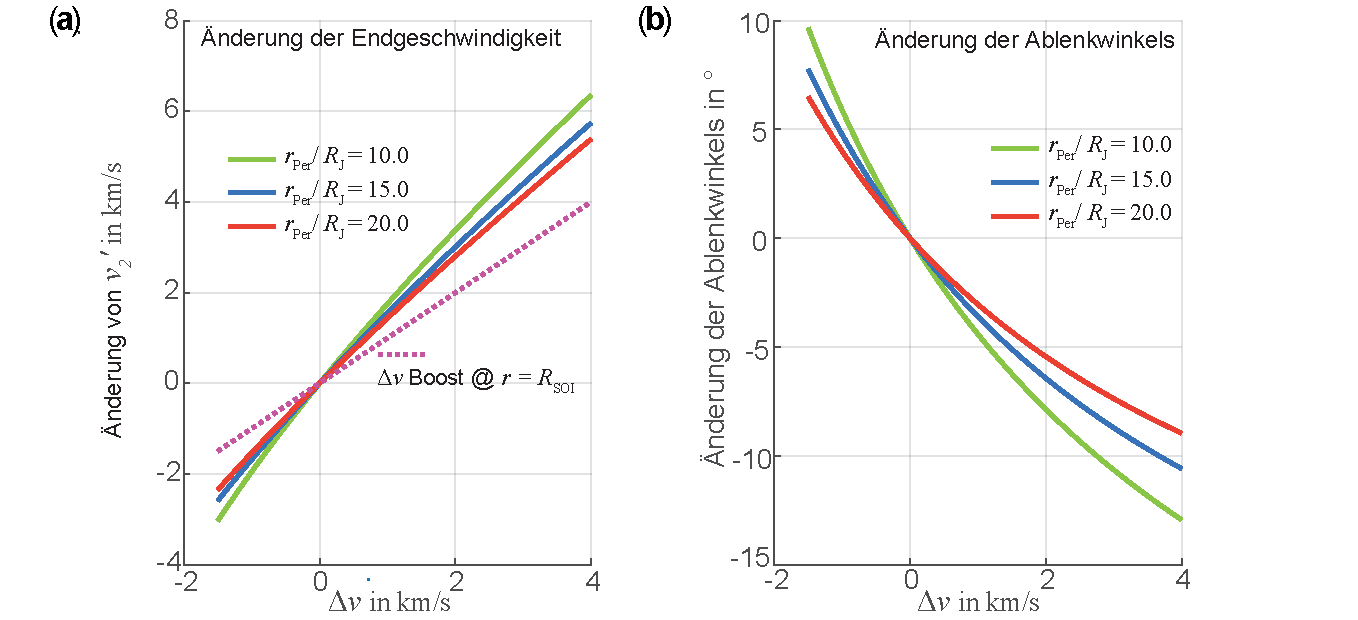
\includegraphics[width=\textwidth]{SwingByOberth01.pdf} 
	\caption[Geschwindigkeits- und Richtungs�nderung beim Gravity-Assist-Man�ver mit zus�tzlichem Schub.]{\fa Geschwindigkeits- und \fb Richtungs�nderung beim Gravity-Assist-Man�ver mit zus�tzlichem Schub am Beispiel Swing-By Jupiter. Man erkennt deutlich, dass der Geschwindigkeitszuwachs, wenn der Boost am Perizentrum erfolgt, deutlich gr��er ist als wenn dieser beim Eintreffen in die SOI des Jupiters erfolgen w�rde. Parameter siehe \mscr~ \mladynref{OberthSwingBy.m}.}
	\label{abb:adyn_swby03}
\end{figure}

\end{sol} 
\textcolor{blue} {$\rightarrow$ zur} \probref{adyn_swingby04}.\\
\noindent\rule[1ex]{\textwidth}{0.5pt} \newpage  \clearpage

%---------------------------------------------------------------------------------------------------


\begin{sol}{prob:adyn_raumfahrtschrott}\label{lsg:adyn_raumfahrtschrott} %Zusatz
\textbf{Raumfahrtschrott}\\

\begin{enumerate}
	\item\textit{\textbf{``Lebensdauer'' von Weltraumm�ll}}\\
	
Die Verweildauer von Weltraumm�ll in einer niedrigen Erdumlaufbahn
(\textit{Low Earth Orbi}t, LEO) wird im Wesentlichen durch den
atmosph�rischen Widerstand bestimmt.
Eine eindeutige Zuordnung \emph{Bahnh�he \(\to\) Lebensdauer} ist nicht
m�glich, da die Lebensdauer stark von
\begin{itemize}
  \item dem \emph{ballistischen Koeffizienten} \(A/m\) (projizierte Fl�che pro Masse),
  \item dem Aerodynamik-Koeffizienten \(C_\text{D}\),
  \item der zeitlich variablen Atmosph�rendichte \(\varrho(h,t)\) (stark variierend mit der Sonnenaktivit�t)
\end{itemize}
abh�ngt. Dennoch lassen sich f�r typische Objekte im All sinnvolle
Absch�tzungen angeben.

F�r ein Objekt der Masse \(m\) und Fl�che \(A\)
sei der aerodynamische Widerstand in erster N�herung (siehe Band I)
\begin{equation}
a_\text{drag}
= \frac{1}{2}\,\varrho(h)\,\,v^2\,C_\text{D}\,\frac{A}{m},
\end{equation}
wobei \(\varrho(h)\) die Atmosph�rendichte in H�he \(h\) und
\(v\) die Bahngeschwindigkeit ist.
Der Faktor \(C_\text{D} A/m\) wird h�ufig durch den
\emph{ballistischen Koeffizienten} charakterisiert:
\begin{equation}
B = \frac{m}{C_\text{D} A}
\quad\Leftrightarrow\quad
C_\text{D}\frac{A}{m} = \frac{1}{B}.
\end{equation}
Typische Werte f�r kleine Satelliten und gr��ere Tr�mmerobjekte liegen im Bereich
\begin{equation}
\frac{A}{m} \sim 10^{-2}\,\si{\meter^2\per\kilo\gram},
\end{equation}
also z.\,B.\ \(A=\SI{10}{\meter^2}\),~\(m=\SI{1000}{\kilo\gram}\)
bei \(C_\text{D} \approx 2.2\).\\


Wir benutzen das exponentielles Atmosph�renmodell (siehe \kap{adyn_drag}).
In guter N�herung kann man die Atmosph�rendichte im LEO
durch ein Exponentialgesetz beschreiben:
\begin{equation}
\varrho(h)
= \varrho_\mathrm{ref}\,\exp\!\left(-\frac{h-h_\mathrm{ref}}{H}\right),
\label{eq:rhoexp}
\end{equation}
wobei \(\varrho_\mathrm{ref}\) eine Referenzdichte bei H�he \(h_\mathrm{ref}\)
und \(H\) eine feste Skalenh�he ist. In einem verbesserten Modell ist \(H\) h�hen- und
zeitabh�ngig und \(\varrho(h,t)\) h�ngt wie erw�hnt stark von der Sonnenaktivit�t ab;
Gleichung~\eqref{eq:rhoexp} ist daher nur ein sehr einfaches Modell.

F�r die Dynamik im Orbit betrachten wir eine einfache Kreisbahn mit Bahnradius $a = R_\text{\earth} + h$, wobei $R_\text{\earth}$ der Erdradius ist.
Die Bahnenergie pro Masse lautet
\begin{equation}
\varepsilon = -\frac{\mu}{2a}
\end{equation}
mit dem Standardgravitationsparameter \(\mu = GM_\text{\earth}\), wobei $M_\text{\earth}$ die Masse der Erde ist.

Durch den Drag wird Energie dissipiert. Die �nderungsrate der
Energie ist $\D \varepsilon /\D t = \mathbf{a}_\text{D}\cdot\mathbf{v} = - a_\text{D}\,v$, da der Widerstand entgegengesetzt zur Geschwindigkeit wirkt.
Andererseits gilt
\begin{equation}
\frac{\mathrm d\varepsilon}{\mathrm d t}
= \frac{\mathrm d}{\mathrm d t}\left(-\frac{\mu}{2a}\right)
= \frac{\mu}{2a^2}\,\frac{\mathrm d a}{\mathrm d t}.
\end{equation}
Damit folgt
\begin{equation}
\frac{\mu}{2a^2}\,\frac{\mathrm d a}{\mathrm d t}
= - a_\text{D}\,v.
\end{equation}
F�r eine Kreisbahn ist $v = \sqrt{\mu/a}$.
Setzt man den Ausdruck f�r \(a_\text{D}\) ein,
\begin{equation}
a_\text{drag}
= \frac{1}{2}\,\varrho(h)\,v^2\,C_\text{D}\,\frac{A}{m},
\end{equation}
so erh�lt man
\begin{equation}
\frac{\mu}{2a^2}\,\frac{\mathrm d a}{\mathrm d t}
= - \frac{1}{2}\,\varrho(h)\,v^3\,C_\text{D}\,\frac{A}{m}.
\end{equation}
Einsetzen von \(v^3 = \left(\mu/a\right)^{3/2}\) liefert
\begin{equation}
\frac{\mathrm d a}{\mathrm d t}
= - \varrho(h)\,C_\text{D}\,\frac{A}{m}\,\sqrt{\mu}\,\sqrt{a}.
\label{eq:adot}
\end{equation}
Da \(h = a - R_\text{\earth}\) ist, h�ngt \(\varrho\) �ber \eqref{eq:rhoexp}
implizit von \(a\) ab. Gleichung~\eqref{eq:adot} l�sst sich numerisch integrieren. Aus einer Starth�he \(h_0\) berechnet man die Zeit bis zu einer
Reentry-H�he \(h_\text{reentry}\) (\zb \SI{122}{\kilo\meter}).\\

Als Gr��enordnungen der Lebensdauer erhalten wir mit 
einem typischen ballistischen Koeffizienten
\(A/m\sim 10^{-2}\,\si{\meter^2\per\kilo\gram}\) und
des erq�hnten groben Modells der Erd-Atmosph�re folgende Werte:

\begin{itemize}
  \item \(h_0 \approx \SI{300}{\kilo\meter}\):
        Lebensdauer von Monaten bis \ca \(\SI{1}{Jahr}\).
  \item \(h_0 \approx \SI{400}{\kilo\meter}\):
        typische Lebensdauer einiger Jahre (\zb~\ca 3-5~ Jahre).
  \item \(h_0 \approx \SI{500}{\kilo\meter}\): \ca 10-20~Jahre.
  \item \(h_0 \approx \SI{600}{\kilo\meter}\): mehrere Jahrzehnte.
  \item \(h_0 \approx \SI{800}{\kilo\meter}\): Jahrhunderte, da die Atmosph�rendichte sehr gering ist.
  \item \(h_0 \gtrsim \SI{1000}{\kilo\meter}\): Jahrhunderte bis Jahrtausende; der atmosph�rischer Drag ist vernachl�ssigbar.
\end{itemize}

Diese Zahlen sind nur Gr��enordnungen. �nderungen der
Sonnenaktivit�t oder des ballistischen Koeffizienten k�nnen die
Lebensdauer leicht um Faktoren von \(2{-}10\) verschieben. 
%Sie entsprechen in etwa der Aussage in \cite{Krag2025}. Wir verweisen f�r Details auf \mscr{} \mladynref{Raumfahrtschrott.m}.\\
%F�r eine quantitative Beispielrechnung l�sst sich 
%Gleichung~\eqref{eq:adot} in Verbindung mit dem
%Exponentialmodell \eqref{eq:rhoexp} numerisch integrieren.
%Setzt man z.\,B.
%\begin{align*}
%\varrho_\mathrm{ref} &\sim 4\times10^{-12}\,\si{\kilo\gram\per\meter^3}
%\quad\text{bei}\quad h_\mathrm{ref} \approx \SI{400}{\kilo\meter},\\
%H &\sim \SI{60}{\kilo\meter},\\
%C_\text{D} &\approx 2{,}2,\qquad \frac{A}{m}\sim 10^{-2}\,\si{\meter^2\per\kilo\gram},
%\end{align*}
%so erh�lt man eine Kurve \(\,T(h_0)\,\) (Lebensdauer als Funktion der
%Starth�he), die qualitativ den oben genannten Gr��enordnungen entspricht.
%Eine Darstellung in doppelt-logarithmischer Form (logarithmische
%Skalierung in der Zeitachse) zeigt, dass die Lebensdauer mit der H�he
%sehr stark anw�chst.\\
%
%Zusammenfassen kann man sagen, das es keinen exakten Zusammenhang zwischen
%Bahnh�he und Lebensdauer gibt; der ballistische Koeffizient \(A/m\), der Widerstandsbeiwert \(C_\text{D}\) und die
%Sonnenaktivit�t spielen eine zentrale Rolle. In einer einfachen Absch�tzung erh�lt man 
%mit der Exponentialatmosph�re und typischen ballistischen Koeffizienten f�r die Verweildauer
%Gr��enordnungen von Jahren bei \(\sim\SI{400}{\kilo\meter}\) \bzw Jahrtausende bei \(\gtrsim\SI{1000}{\kilo\meter}\).

\item\textit{\textbf{Beseitigung von Weltraumm�ll mit Lasern}}\\
	
Wir betrachten nun ein ideales, kugelf�rmiges St�ck Weltraumm�ll
mit Durchmesser \(\SI{10}{\centi\meter}\) in einer kreisf�rmigen Bahn
in \(\SI{800}{\kilo\meter}\) H�he �ber der Erdoberfl�che.
Ziel ist es, durch Laserablation die Bahn so zu �ndern, dass
das Perig�um auf etwa \(\SI{300}{\kilo\meter}\) abgesenkt wird.
In dieser H�he ist der atmosph�rische Widerstand gro� genug,
dass das Objekt typischerweise innerhalb von deutlich weniger als 5 Jahren 
wieder in die Atmosph�re eintritt (genaue Lebensdauer
h�ngt vom Atmosph�renmodell und dem ballistischen Koeffizienten ab) und vergl�ht.

Wir wollen eine grobe Absch�tzung der erforderlichen Laserenergie
f�r die Verwendung von Laserablation zur Weltraumm�ll-Beseitigung machen.

\subparagraph{Orbitdynamik}

Wir modellieren die Erde mit Radius $R_\text{\earth} \approx \SI{6371e3}{\meter}$
und Standardgravitationsparameter
$\mu_\text{\earth} \approx \SI{3.986e14}{\meter^3\per\second^2}$.
Die Ausgangsbahn sei kreisf�rmig mit H�he $h_0 = \SI{800e3}{\meter}$, und damit $r_0 = R_\text{\earth} + h_0$.
Die Kreisbahngeschwindigkeit ist
\begin{equation}
v_{\text{K,0}}
= \sqrt{\frac{\mu_\text{\earth}}{r_0}}.
\end{equation}
Als Zielbahn soll eine elliptische Bahn mit Apog�um in \(\SI{800}{\kilo\meter}\)
und Perig�um in \(\SI{300}{\kilo\meter}\) angenommen werden:
\[
h_\text{P} = \SI{300e3}{\meter},\quad
r_\text{P} = R_\text{\earth} + h_\text{P},\quad
r_\text{A} = r_0.
\]
Die gro�e Halbachse dieser lautet dann $a = (r_\text{P} + r_\text{A})/2$.
Die Geschwindigkeit im Apog�um dieser elliptischen Bahn ergibt sich
aus der \textit{vis-viva-Gleichung}\index{vis-viva-Gleichung} \eqref{eq:hm_vis-viva}:
\begin{equation}
v_\text{A}
= \sqrt{\mu_\text{\earth}\left(\frac{2}{r_\text{A}} - \frac{1}{a}\right)}.
\end{equation}
Wir brauchen  also am Apog�um eine retrograde Geschwindigkeits�nderung \(\Delta v\), um von der
kreisf�rmigen in die elliptische Bahn zu wechseln:
\begin{equation}
\Delta v = v_{\text{K,0}} - v_\text{A}.
\end{equation}
Mit den Zahlenwerten erhalten wir
%\begin{align}
%r_0 &= R_\text{earth} + \SI{800e3}{\meter},\\
%r_\text{P} &= R_\text{earth} + \SI{300e3}{\meter},\\
%a &= \frac{r_0 + r_\text{p}}{2}.
%\end{align}
%Damit erh�lt man numerisch
$ v_{\text{c,0}} \approx \SI{7456}{\meter\per\second},\,\,v_\text{A} \approx \SI{7320}{\meter\per\second},\,\, \Delta v \approx \SI{136}{\meter\per\second}$.
Dieses \(\Delta v\) gen�gt, um das Perig�um auf \ca \(\SI{300}{\kilo\meter}\)
abzusenken. 
%Noch niedrigere Zielh�hen (z.\,B. \(\SI{200}{\kilo\meter}\))
%w�rden ein etwas gr��eres \(\Delta v\) erfordern (Gr��enordnung
%\(\sim \SI{160}{\meter\per\second}\)).\\

Wir nehmen an, dass das Objekt eine Kugel aus Aluminium
mit Durchmesser \(d = 2r = \SI{10}{\centi\meter}\) ist.
%Das Volumen der Kugel ist
%\begin{equation}
%V = \frac{4}{3}\pi r^3.
%\end{equation}
Mit einer typischen Dichte f�r Aluminium von
\(\varrho \approx \SI{2700}{\kilo\gram\per\meter^3}\) ist die Masse
$m = \varrho V \approx \SI{1.4}{\kilo\gram}$.
%In der Realit�t kann die Masse je nach Geometrie und Material
%stark variieren; \(\SI{1}{\kilo\gram}\) bis einige \(\SI{}{kg}\) f�r
%\(\sim\SI{10}{\centi\meter}\)-Objekte ist jedoch plausibel als Gr��enordnung.\\

Der f�r die Bahn�nderung notwendige Impuls ist
\begin{equation}
I_\text{ges} = m\,\Delta v \approx \SI{1.9e2}{\newton\second} \,.
\end{equation}

\subparagraph{Laserablation und Impuls-Kopplungskoeffizient}

Bei Laserablation wird eine d�nne Oberfl�chenschicht verdampft
und bildet einen Plasmastrahl. Der R�cksto� liefert den gew�nschten
Impuls. Als praktische Kenngr��e wird h�ufig der
\emph{Impuls-Kopplungskoeffizient} \(C_m\) verwendet:
\begin{equation}
C_\text{abl} = \frac{\Delta I}{E_\text{Laser}},
\end{equation}
also Impuls pro eingestrahlter Laserenergie. Die Einheit ist
\(\si{\newton\second\per\joule}\).

Typische Werte f�r \(C_\text{abl}\) bei Nanosekundenimpulsen im
\(\SI{1}{\micro\meter}\)-Bereich und geeigneten Energiewerten
liegen in der Gr��enordnung
\[
C_\text{abl}\sim 10^{-4} \dots 10^{-3}\,\si{\newton\second\per\joule},
\]
je nach Material, Wellenl�nge, Pulsdauer und Energie.

Die erforderliche Laserenergie zur Erzeugung des Gesamtimpulses
\(I_\text{ges}\) ist $E_\text{Laser} = I_\text{ges}/C_\text{abl}$.
Mit \(I_\text{ges} \approx \SI{1.9e2}{\newton\second}\) und
\(C_\text{abl} \approx \SI{3e-4}{\newton\second\per\joule}\) ergibt sich
\begin{align}
E_\text{Laser}
&\approx \frac{\SI{1.9e2}{}}{\SI{3e-4}{}}\,\SI{}{\joule} \approx \SI{6.4e5}{\joule} \approx \SI{0.64}{\mega\joule}\,.
\end{align}

F�r andere plausible Werte von \(C_\text{abl}\) ergibt sich z.\,B.
\begin{align*}
C_\text{abl} &= \SI{1e-4}{\newton\second\per\joule}
&&\Rightarrow&
E_\text{Laser} &\approx \SI{1.9e6}{\joule}
\approx \SI{1.9}{\mega\joule},\\
C_\text{abl} &= \SI{1e-3}{\newton\second\per\joule}
&&\Rightarrow&
E_\text{Laser} &\approx \SI{1.9e5}{\joule}
\approx \SI{0.19}{\mega\joule}.
\end{align*}

Wir erhalten also eine grobe Bandbreite von $E_\text{Laser} \sim 0.2 \dots 2\,\si{\mega\joule} $ f�r ein \(\SI{10}{\centi\meter}\)-Objekt mit \(\sim\SI{1.4}{\kilo\gram}\)
Masse und \(\Delta v \sim \SI{136}{\meter\per\second}\).

Setzen wir \(E_\text{Laser} \approx \SI{0.64}{\mega\joule}\) an,
so entspricht dies $E\text{el} = E_\text{Laser}/\eta$, wobei \(\eta\) der Gesamtwirkungsgrad vom Stromnetz bis zum
Zielobjekt ist (Laser-Wirkungsgrad, Strahlf�hrung, atmosph�rische
Verluste etc.). Selbst bei einem eher optimistischen Gesamtwirkungsgrad
$\eta \sim 10\%$ ergibt sich
\begin{equation}
E_\text{el} \approx \SI{1.8}{\kilo\watt\hour}\,.
\end{equation}
Das ist energetisch durchaus handhabbar, zumal sich die Ablation
�ber viele einzelne Impulse und zahlreiche Uml�ufe verteilen kann.\\

In einem realistischen Szenario w�rde man das Objekt bei jedem
�berflug des Laserstandorts (bzw.\ des Laser-Satelliten)
f�r kurze Zeit im Fokus haben und pro Passage eine gewisse Anzahl
von Impulsen einbringen. Der Gesamtimpuls von \ca
\(\SI{200}{\newton\second}\) kann also auf viele hundert oder tausende
Impulse verteilt werden, etwa in der Gr��enordnung
\begin{equation}
\Delta I_\text{pro Impuls} \sim 10^{-2} \dots 10^{-1}\,\si{\newton\second},
\end{equation}
je nach Impulsenergie.\\

Die gemachte Absch�tzung enth�lt
mehrere idealisierende Annahmen:
\begin{itemize}
  \item Das Objekt ist eine homogene Aluminiumkugel; reale Tr�mmer
        haben komplexe Geometrie und Materialkombinationen.
  \item Der Impuls-Kopplungskoeffizient \(C_\text{abl}\) h�ngt stark von
        verschiedenen Parametern ab.
  \item Die Orbitdynamik ist idealisiert (keine St�rungen, kein zus�tzlicher aerodynamischer Drag
        w�hrend der Absenkphase).
\end{itemize}

Bei der Bahn�nderung von Weltraumm�ll durch Laserbestrahlung stellt sich die Frage, ob neben dem R�cksto� durch die Ablationsplasmawolke auch der reine Photonenimpuls des Laserstrahls ber�cksichtigt werden muss.\\
Im eigentlichen Ablationsregime ist der Photonenimpuls in der Regel gegen�ber dem Ablationsr�cksto� vernachl�ssigbar. Unterhalb der Ablationsschwelle kann er dagegen der f�hrende Effekt sein. Wir wollen das quantitativ absch�tzen:
Allgemein kann man mit einem dimensionslosen Kopplungsfaktor \(C_R\) der Impuls�bertrag  als (siehe Band V):
\begin{align}
	\Delta I_\text{photon} = C_\text{R} \frac{E_\text{Laser}}{c}\, \qquad 1 \le  C_\text{R}R \le 2
\end{align}
f�r den Bereich zwischen idealer Absorption und idealer Spiegelung schreiben.
Daraus folgt f�r den Impuls pro Joule bei Absorption
\[
\lk \frac{\Delta I_\text{photon}}{E_\text{Laser}}\rk_\gamma \approx \SI{3.33e-9}{\newton\second\per\joule}\,,
\]
und bei perfekter Reflexion maximal der doppelte Betrag, was sehr klein ist.
Das Verh�ltnis von Ablationsimpuls zu Photonenimpuls ist
\[
\frac{\Delta I_\text{abl}}{\Delta I_\text{photon}} = \frac{C_\text{abl} E_\text{Laser}}{C_\text{R} E_\text{Laser}/c} = \frac{C_\text{abl}}{C_\text{R}}c\,.
\]
Mit $C_\text{abl} = \SI{1e-5}{\newton\second\per\joule}$ erh�lt man f�r $\Delta I_\text{abl}/\Delta I_\text{photon}$ einen Wert von \ca $\SI{3e3}{}$.
Der Ablationsr�cksto� ist also typischerweise um drei bis vier Gr��enordnungen gr��er als der reine Photonenimpuls.\\

Trotz unserer gemachten Vereinfachungen liefert die Rechnung eine sinnvolle
Gr��enordnung: F�r ein \(\SI{10}{\centi\meter}\)-Objekt in \(\SI{800}{\kilo\meter}\)
H�he liegt die erforderliche Laserenergie zur Absenkung des Perig�ums
auf etwa \(\SI{300}{\kilo\meter}\) typischerweise im Bereich einiger
\(\SI{}{\mega\joule}\) auf dem Zielobjekt, was technisch prinzipiell
machbar ist, wenn man die Ablation �ber viele Uml�ufe verteilt. In Bezug auf reine Energiegr��enordnungen erscheint
ein Laser-basiertes Deorbiting einzelner \(\SI{10}{\centi\meter}\)-Objekte
prinzipiell realistisch. Die eigentlichen Herausforderungen liegen eher
in Strahlf�hrung, Zielverfolgung und Systemkomplexit�t.
Insbesondere haben wir in unseren Rechnungen unber�cksichtigt gelassen, wie die Laserenergie von der Erde so zum Tr�mmerobjekt gebracht werden kann, \dh ausgerichtet und fokussiert werden kann, dass die gesamte \bzw ein Gro�teil der von der Erde abgestrahlten Energie das relativ kleine Tr�mmerobjekt trifft. Mit solchen, im Wesentlichen optischen Fragen, wollen wir uns n�her im Band V besch�ftigen.  

%Nicht zuletzt soll erw�hnt werden, dass es f�r die Methode noch eine  Reihe rechtlicher und politischer Rahmenbedingungen zu kl�ren gilt.

%Zusammenfassung 
%
%\begin{itemize}
  %\item Ben�tigtes \(\Delta v\) zur Absenkung des Perig�ums von
        %\(\SI{800}{\kilo\meter}\) auf \(\SI{300}{\kilo\meter}\):
        %\(\Delta v \approx \SI{136}{\meter\per\second}\).
  %\item Masse eines idealisierten \(\SI{10}{\centi\meter}\)-Aluminiumfragments:
        %\(m \approx \SI{1.4}{\kilo\gram}\).
  %\item Gesamtimpulsbedarf:
        %\(I_\text{ges} \approx \SI{2e2}{\newton\second}\).
  %\item Bei typischen Werten f�r den Impuls-Kopplungskoeffizienten
        %\(C_m \sim 10^{-4} \dots 10^{-3}\,\si{\newton\second\per\joule}\)
        %ergibt sich eine ben�tigte Laserenergie auf dem Zielobjekt von
        %\[
        %E_\text{Laser} \sim 0{,}2 \dots 2\,\si{\mega\joule}.
        %\]
%\end{itemize}
%
\end{enumerate}

\end{sol} 
\textcolor{blue} {$\rightarrow$ zur} \probref{adyn_raumfahrtschrott}.\\
\noindent\rule[1ex]{\textwidth}{0.5pt} 

%---------------------------------------------------------------------------------------------------

\newpage
\begin{sol}{prob:adyn_proxima_centauri}\label{lsg:adyn_proxima_centauri} %Zusatz
\textbf{Starshot and Starlight}\\


Wir verweisen auf \cite{Umrigar2025} und danken den Autoren f�r dieses instruktive physikalische Problem.\\

\end{sol} 
\textcolor{blue} {$\rightarrow$ zur} \probref{adyn_proxima_centauri}.\\
\noindent\rule[1ex]{\textwidth}{0.5pt} 



%---------------------------------------------------------------------------------------------------

\newpage
\begin{sol}{prob:adyn_waterrocket}\label{lsg:adyn_waterrocket} %Zusatz
\textbf{Wasserrakete}\\

Gegeben sind folgende Parameter:
\begin{itemize}
  \item Wasservolumen $V_\text{W0}$, Luftvolumen �ber dem Wasser $V_\text{A0}$, Flaschenvolumen $V_\text{F}=V_\text{W0}+V_\text{A0}$.
  \item Druck der komprimierten Luft $p_0$ als Absolutdruck.
  \item D�sendurchmesser $d_\text{N}$ mit Querschnitt $A_\text{N}=\pi(d_\text{N}/2)^2$.
  \item Abschusswinkel $\theta$ (konstant als Schubrichtung angenommen).
  \item Trockenmasse $m_\mathrm{F}$ (Flasche+Nase+Finnen), aerodynamische Parameter $C_\text{D}$ und Referenzfl�che $A_\mathrm{ref}$.
\end{itemize}

Konstanten:
Wasserdichte $\varrho_\text{W}\approx 1000\,\mathrm{kg/m^3}$, Luftdichte $\varrho_\mathrm{A}\approx 1.2\,\mathrm{kg/m^3}$,
adiabatischer Exponent der Luft $\gamma\approx 1.4$,
Umgebungsdruck $p_\mathrm{Luft}\approx 101325\,\mathrm{Pa}$.
Der Ausflussbeiwert der D�se liege $C_\text{D,N}$ im Intervall $[0.8,0.95]$.

In der Wasser-Schubphase (Blowdown), \dh w�hrend Wasser ausstr�mt, vergr��ert sich das Luftvolumen $V_\text{A}(t)$, und der Flaschendruck f�llt adiabatisch:
\begin{equation}
p(t)=p_0\left(\frac{V_\text{A0}}{V_\text{A}(t)}\right)^\gamma.
\end{equation}
Der antreibende Differenzdruck ist $\Delta p(t)=\max(p(t)-p_\mathrm{L},0)$.

F�r die Strahlgeschwindigkeit (wir nehmen die Bernoulli-L�sung (siehe Band I) mit Ausflussbeiwert gilt
\begin{equation}
v_\text{ex}(t)=C_\text{D,N}\sqrt{\frac{2\,\Delta p(t)}{\varrho_\text{W}}}.
\end{equation}
Damit folgen Volumenstrom \bzw  Massenstrom des Wassers:
\begin{equation}
\dot V(t)=A_n v_\text{ex}(t), ~~ \rightarrow~~ \dot m_\text{W}(t)=\varrho_\text{W} A_\text{N} v_\text{ex}(t).
\end{equation}
Eine einfache Schubn�herung in der Wasserphase ist die Impulsbilanz
\begin{equation}
T(t)\approx \dot m_\text{W}(t)\, v_\text{ex}(t).
\end{equation}
Diese ist gerechtfertigt, da der zus�tzliche Druckterm $(p_\text{ex}-p_\mathrm{amb})A_n$ bei freiem Wasserstrahl meist klein gegen�ber $\dot m v_\text{ex}$ ist. 
Die Luftvolumen�nderung ist identisch mit dem abgeflossenen Wasservolumen:
\begin{equation}
\dot V_\text{A}(t)=\dot V(t)=A_n v_\text{ex}(t).
\end{equation}
Die Wasserphase endet bei $V_\text{A}(t)=V_\text{F}$ (Wasser ist leer) oder wenn $\Delta p(t)=0$.
Die Wassermasse ist $m_w(t)=\varrho_w V_\text{W}(t)$ und f�llt mit
\begin{equation}
\dot m_\text{W}(t)=-\varrho_\text{W} A_\text{N} v_\text{ex}(t).
\end{equation}
Die Gesamtmasse sei (w�hrend der Wasserphase)
\begin{equation}
m(t)=m_\mathrm{F}+m_\text{W}(t)+m_\mathrm{A},
\end{equation}
wobei $m_\mathrm{A}$  als konstant angenommen werden kann.

Der aerodynamischer Widerstand wird quadratisch angesetzt (wir haben nach einfacher Absch�tzung eine gro�e Reynolds-Zahl, die Turbulenz ergibt):
\begin{equation}
\mathbf{F}_\text{D}=\frac12\varrho_\mathrm{air} C_\text{D} A_\mathrm{ref} \, |\vec{v}|\,\vec{v}.
\end{equation}
Die Schubrichtung wird als konstant entlang des Abschusswinkels $\theta$ angenommen (Das setzt voraus, dass zumindest in der Schubphase die Rakete ihrer Abschussrichtung beibeh�lt,  genauer w�re eigentlich wenn Schubrichtung der Tangente an die Bahn entspricht.)
\begin{equation}
\vec{T}(t)=T(t)\begin{pmatrix}\cos\theta\\ \sin\theta\end{pmatrix}.
\end{equation}
Dann lautet die Bewegungsgleichung:
\begin{equation}
m(t)\, \dot{\mathbf{v}}=\vec{T}(t)-\vec{F}_\text{D} - m(t)\,g\begin{pmatrix}0\\1\end{pmatrix}.
\end{equation}
Die Numerische Integration erfolgt in Zeitschritten $\Delta t$ mit explizitem Euler-Verfahren oder der \matlab~\odevf-Rotine.
Ausgegeben werden die Trajektorien $(x(t),y(t))$, $(t,z(t))$, die maximale H�he $z_\mathrm{max}$, die Flugzeit $t_\mathrm{impact}$ und die Reichweite $x(t_\mathrm{impact})$ (bei $z=0$). Ergebnisse haben wir f�r die Werte unserer Modellraket (Tabelle \ref{tab:adyn_param_wasserrakete}) zeigen wir in \figref{adyn_WaterRocket}.\\
\begin{table}%tab1
\smallskip
\begin{tabular}{L{4cm}L{4cm}}
\svhline\noalign{\smallskip}
\noalign{\smallskip}
\textbf{Gr��e} & \textbf{Wert} \\
\noalign{\smallskip}\svhline\noalign{\smallskip}
Wasservolumen bei $t=0$ & $0.375\,\mathrm{l}$ \\
Luftvolumen bei $t=0$   & $0.375\,\mathrm{l}$ \\
Masse der Flasche       & $70.00\,\mathrm{g}$ \\
Druck bei $t=0$         & $650000.00\,\mathrm{Pa}$ \\
D�sendurchmesser        & $5.00\,\mathrm{mm}$ \\
$C_\text{D}$-Wert       & $0.40$ \\
Querschnitt             & $19.63\,\mathrm{cm^2}$ \\
Winkel                  & $55.00^\circ$ \\
\hline
Reichweite              & $86.1\,\mathrm{m}$ \\
Maximale H�he           & $33.7\,\mathrm{m}$ \\
Flugzeit                & $5.79\,\mathrm{s}$ \\
\noalign{\smallskip}
\svhline\noalign{\smallskip}
\end{tabular}
\caption{Parameter und Messwerte der Wasserrakete}
\label{tab:adyn_param_wasserrakete}
\end{table}
\begin{figure}
	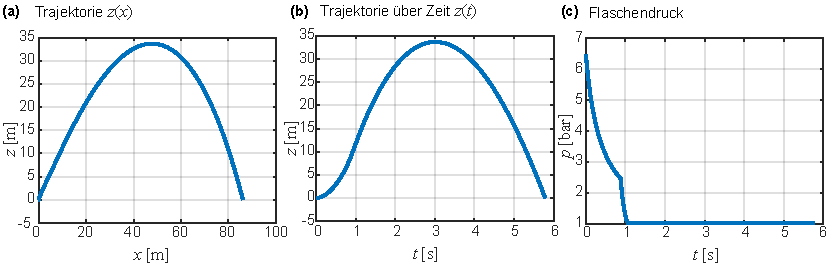
\includegraphics[scale=1]{WaterRocket.pdf} 
	\caption[Trajektorie einer Wasserrakete.]{Trajektorie einer Wasserrakete. Parameter siehe Tabelle \ref{tab:adyn_param_wasserrakete} und \mscr~ \mladynref{WaterRocket.m}.}
	\label{abb:adyn_WaterRocket}
\end{figure}

Bei der numerischen Integration m�ssen wir auf  einen ``stetigen'' �bergang zwischen Wasser- und Gasphase achten, denn im einfachen Modell wird beim Erreichen von $m_\text{W}=0$ abrupt von der Wasser-Schubformel auf die Gas-Schubformel umgeschaltet. Dadurch w�rde im Schub-Zeit-Diagramm unter Umst�nden 
eine unphysikalisch Diskontinuit�t auftreten. Zur numerischen Regularisierung verwenden wir deshalb eine kleine �bergangszone f�r sehr kleine Restwassermassen. Sei
$ m_{\text{W}0}=\varrho_\text{W} V_{\text{W}0}$ die Anfangswassermasse und $\varepsilon \ll 1$ ein kleiner Bruchteil, \zb $0.02$, dann wird f�r
$m_\text{W} \le \varepsilon\, m_{\text{W}0}$
ein ``glatter'' Mischfaktor
\begin{align}
	w = \frac12 \lek 1+\cos\!\lk \pi \lk 1-\frac{m_\text{W}}{\varepsilon m_{\text{W}0}}\rk \rk \rek
\end{align}
verwendet. Dann gilt:
\[
w=1 \quad \text{bei} \quad m_\text{W}=\varepsilon m_{\text{W}0}, \qquad w=0 \quad \text{bei} \quad m_\text{W}=0\,.
\]
Der Schub wird in dieser Zone als gewichtete Summe geschrieben:
$T = w\,T_\mathrm{W} + (1-w)\,T_\mathrm{A}$, Analog kann auch der Massenstrom gegl�ttet werden:
\[
\dot m = w\,\dot m\text{W} + (1-w)\,\dot m_\text{A}.
\]
Diese Vorgehensweise ist in erster Linie eine numerische Regularisierung und kein
vollst�ndiges physikalisches Zweiphasenmodell, f�hrt aber zu einer realistischen und numerisch stabilen
Schubkurve.\\

Die �bereinstimmung der numerischen Rechnung mit den Beobachtungen ist damit relativ gut, insbesondere wenn man die gemachten groben N�herungen ber�cksichtigt.\\

Wir wollen das Ganze jetzt noch mit einer so genannten Fehlerlandkarte (\textit{Error-Map}) �berpr�fen. Das Ziel ist, aus den experimentellen Messdaten Reichweite, maximale H�he, Flugzeit 
($R_{\mathrm{exp}}, H_{\mathrm{exp}}$ und $T_{\mathrm{exp}}$ )
die plausiblen unbekannten Modellparameter zu bestimmen. 
Im unserem Fall werden als freie Parameter der aerodynamische Widerstandsbeiwert  $C_\text{D}$ und der absolute Anfangsdruck $p_0$ genommen. 
Alle �brigen Gr��en, insbesondere die geometrischen Gr��en der Rakete, werden als bekannt angenommen.
Die Methode basiert auf einer systematischen Abtastung des Parameterraums und der Bewertung der jeweiligen Parameterkombination durch eine Fehlerfunktion.
Das physikalische Modell, im \mscr{}~ durch 
$\textcolor{mygreen}{\texttt{waterRocketSim}}$ 
realisiert, definiert eine Abbildung der Art
\begin{align}
	(C_\text{D}, p_0) ;\longmapsto; \lk R_{\mathrm{sim}}, H_{\mathrm{sim}}, T_{\mathrm{sim}}\rk \,.
\end{align}
Zum Vergleich zwischen Simulation und Messung werden relative Fehler definiert:
\begin{align*}
	e_R &= \frac{R_{\mathrm{sim}} - R_{\mathrm{exp}}}{R_{\mathrm{exp}}}\,,\quad e_H = \frac{H_{\mathrm{sim}} - H_{\mathrm{exp}}}{H_{\mathrm{exp}}}\,,\quad
	e_T = \frac{T_{\mathrm{sim}} - T_{\mathrm{exp}}}{T_{\mathrm{exp}}}\,.
\end{align*}
Diese Normierung hat den Vorteil der dimensionslosen Darstellung und der gleichen Gewichtung der Messwerte unabh�ngig von der Gr��enordnung.

\begin{figure}
	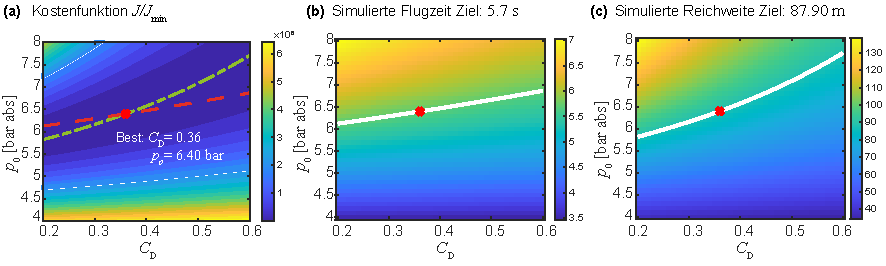
\includegraphics[scale=1]{WaterRocket02.pdf} 
	\caption[Error-Map einer Wasserrakete f�r die Variablen Parameter $p_0$ und $C_\text{D}$.]{Error-Map einer Wasserrakete f�r die variablen Parameter $p_0$ und $C_\text{D}$. \fa Error-Map mit Schnittpunkt Flugzeit und Reichweite als Messwerte der Wasserrakete \fb Zielsimulation auf die Messwert Flugzeit der Wasserrakete, \fc Zielsimulation auf die Messwert Reichweite der Wasserrakete. Parameter siehe Tabelle \ref{tab:adyn_param_wasserrakete} und \mscr~ \mladynref{WaterRocket.m}.}
	\label{abb:adyn_WaterRocket02}
\end{figure}

Die Fehler werden zu einer skalaren Kostenfunktion kombiniert:
\begin{align}
	J(C_\text{D},p_0) = w_R e_R^2 + w_H e_H^2 + w_T e_T^2\,~~\text{mit Gewichtungsfaktoren}~~w_R, ~ w_H, ~ w_T \ge 0\,.
\end{align}
$J=0$ entspricht perfekter �bereinstimmung, kleine Werte von $J$ bedeuten gute Anpassung.
Der Parameterraum wird auf einem Gitter diskretisiert, woraus sich ein zweidimensionales Raster
$[C_{\text{D},i}, p_{0,j}] $ f�r $i=1,\dots,N,~ j=1,\dots,M$ ergibt.
F�r jedes Gitterelement wird die Simulation durchgef�hrt und aus den relativen Fehlern $e_R, e_H, e_T$ die Kostenfunktion ausgewertet:
Aus der erhaltenen Matrix ergibt sich der beste Parametersatz durch Minimierung.
In der Error-Map wird die Funktion $J(C_\text{D},p_0)$ \zb durch eine Farbkarte (\textit{Heatmap}) dargestellt.
Zus�tzlich werden h�ufig geplottet $R_{\mathrm{sim}}(C_\text{D},p_0)$, $T_{\mathrm{sim}}(C_\text{D},p_0)$ und $H_{\mathrm{sim}}(C_\text{D},p_0)$.
Besonders aussagekr�ftig sind die Konturen $R_{\mathrm{sim}} = R_{\mathrm{exp}}$, $T_{\mathrm{sim}} = T_{\mathrm{exp}}$ und $H_{\mathrm{sim}} = H_{\mathrm{exp}}$.
Schnittpunkte dieser Kurven im Parameterraum entsprechen konsistenten L�sungen, mehrere Schnittpunkte bedeuten Nicht-Eindeutigkeit und  keine Schnittpunkte deuten auf Modellabweichungen hin.\\

Die Error-Map ist ein zentrales Werkzeug zur Modellvalidierung und Parameteridentifikation und liefert eine hilfreiche diskrete Approximation der Funktion $J(C_\text{D},p_0)$ dar, welche den Abstand zwischen Simulation und Experiment misst.
Sie erlaubt eine visuelle Analyse des Parameterraums, eine Bestimmung optimaler Parameter und die Identifikation von Unsicherheiten und Korrelationen.\\

\subparagraph{Modellverfeinerungen und zus�tzliche Problemstellungen:}

In einer Verfeinerung des Modells k�nnte man ber�cksichtigen:
\begin{enumerate} [1)]
	\item die Beschreibung der Rakete als starren K�rper mit ver�nderlichen Schwerpunkt, 
	\item den Pitch (Nickbewegung) der Richtung des Schubs durch die Wirkung Schwerkraft/Reibung auf die Rakete,
	\item den Auftrieb der Rakete und
	\item die Rotation der Rakete um die L�ngsachse (hervorgerufen durch die seitlichen ``Flossen'').
\end{enumerate}

Eine weitere sch�ne �bung ist der Vergleich mit der Trajektorie eines schr�gen Wurfs, der die gleiche H�he und Reichweite erreicht. 
Man vergleiche insbesondere die dazu notwendige  Abwurfgeschwindigkeit. (Wir verweisen auch auf die �bung 1.41 in Band I Mechanik).
Wir finden interessanterweise, dass man bei einer Abwurfgeschwindigkeit von udn einem Abwurfwinkel eine Trajektorie $z(x)$ erh�lt, die in etwa mit der Trajektorie der Wasserrakete �bereinstimmt und zwar sowohl bei Scheitelh�he als auch Reichweite.
Das Zeitverhalten ist aber leicht unterschiedlich (die Rakete muss ja erst beschleunigt werden), so dass der Wurf eine um 0.5 s verk�rzte Flugzeit hat. Siehe dazu die \mscr{}e \mladynref{WaterRocket.m} und \mladynref{WaterRocketVergleichWurf.m}.

%Wir wollen die Punkte 1) bis 3) gemeinsam angehen und die Rakete nicht mehr als Punktmasse behandeln, sondern als starren K�rper (in der $x$-$z$-Ebene).
%Dadurch k�nnen zus�tzlich zur translatorischen Bewegung auch die Orientierung und die Nickbewegung beschrieben werden.
%
%Das Modell umfasst:
%\begin{itemize}
%\item Translation des Schwerpunkts in der Ebene $(x,z)$,
%\item Rotation der Rakete mit Winkel $\theta$,
%\item Winkelgeschwindigkeit $\omega=\dot\theta$,
%\item zeitabh�ngige Gesamtmasse $m(t)$,
%\item zeitabh�ngigen Schwerpunkt $x_{CG}(t)$ entlang der Raketenachse,
%\item zeitabh�ngiges Tr�gheitsmoment $I_{CG}(t)$.
%\end{itemize}
%
%Der Zustandsvektor sei
%\[
%\vec{Y}(t)= \lek x, z, v_x, v_z, \theta, \omega, m_\text{W},  m_\text{A} \rek^\text{T}\,.
%\]
%Dabei ist $\theta$ die Orientierung der Raketenachse gegen die $x$-Achse und ,
%$\omega$ die Nickrate. Die anderen Parameter wurden bereits oben eingef�hrt.
%Die Raketenachse ist durch den Einheitsvektor
%\[
%\vec e_\text{R}=
%\begin{pmatrix}
%\cos\theta\\
%\sin\theta
%\end{pmatrix}
%\]
%gegeben.
%Ein dazu senkrechter Einheitsvektor ist
%\[
%\vec e_n=
%\begin{pmatrix}
%-\sin\theta\\
%\cos\theta
%\end{pmatrix}.
%\]
%Die Geschwindigkeit des Schwerpunkts ist
%\[
%\vec v=
%\begin{pmatrix}
%v_x\\
%v_z
%\end{pmatrix},
%\qquad
%V=\|\mathbf v\|=\sqrt{v_x^2+v_z^2}.
%\]
%Der Flugbahnwinkel (siehe \kap{}) ist $\gamma=\operatorname{atan2}(v_y,v_z)$.
%Der Anstellwinkel (ebenfalls Verweis auf\kap{}) der Rakete relativ zur Flugrichtung wird definiert als $\alpha=\theta-\gamma$.
%F�r kleine Winkel ist $\alpha$ der zentrale aerodynamische P
%%Die Gesamtmasse ist
%%\[
%%m(t)=m_{\mathrm{F}} + m_\text{W}(t) + m_\text{W}(t) + m_a(t).
%%\]a(t).
%%\]
%%
%Die Lage des Schwerpunkts entlang der Raketenachse werde durch $x_\text{S}(t)$
%beschrieben. Sie kann aus den Teilmassen berechnet werden:
%\[
%x_\text{S}(t)=\frac{\sum_i m_i(t)x_i}{\sum_i m_i(t)},
%\]
%wobei man typischerweise die Rakete in die Bestandteile trockene Flasche, Wasserf�llung, Luft, Nase und Flossen zerlegt.
%Das Tr�gheitsmoment um den Schwerpunkt ist
%\[
%J_\text{S}(t)=\sum_i \lk J_i^{(\mathrm{eig})} + m_i(t) \lek (x_i-x_\text{S}(t)\rek^2\rk\,.
%\]
%Es wirken im Wesentlichen vier Kr�fte:
%\begin{enumerate} [(a)]
	%\item Schwerkraft\\
			%\[
		%\mathbf F_g=
		%\begin{pmatrix}
		%0\\
		%-\,m(t)g 
		%\end{pmatrix}.\]
	%\item Schub\\
	%Der Schub wirkt entlang der Raketenachse: $\mathbf F_T = T(t)\,\vec e_\text{R}$.
	%\item Luftwiderstand\\
	%Der Widerstand wirkt entgegen der Flugrichtung:
		%\[
		%\mathbf F_D
		%=
		%-\frac12 \rho_{\mathrm{air}} V^2 A_{\mathrm{ref}} C_\text{D} \,\vec e_v,
		%\]
		%wobei $\mathbf e_v=\frac{\mathbf v}{V}$ f�r $V>0$.
	%\item Normalkraft\\
		%Die aerodynamische Normalkraft wird f�r kleine Anstellwinkel modelliert durch $N=\frac12 \rho_{\mathrm{A}} V^2 A_{\mathrm{ref}}\, C_{N\alpha}\,\alpha$. Sie wirkt senkrecht zur Raketenachse, \dh $\vec{F}_N = N\,\vec{e}_n$.
%\end{enumerate}
%
%Die Translation des Schwerpunkts folgt der Newton-Bewegungsgleichung. 
%\begin{align}
	%m(t)\,\dot{\mathbf v} &= \mathbf F_T + \mathbf F_D + \mathbf F_N + \mathbf F_g\,\\
%\end{align}
%\bzw in Komponentenschreibweise:
%\begin{align}
%\begin{split}
	%\dot x   &= v_x\,,\\
	%\dot z 	 &= v_z\,,\\
	%\dot v_x &= \frac{F_{T,x}+F_{D,x}+F_{N,x}}{m(t)}\,,\\
	%\dot v_z &= \frac{F_{T,y}+F_{D,y}+F_{N,y}}{m(t)} - g\,.
%\end{split}
%\end{align}
%Die Rotationsgleichung um den Schwerpunkt lautet
%\begin{align}
	%I_\text{S}(t)\,\dot\omega = M(t)~~~\text{mit}~~~\dot\theta=\omega\,.
%\end{align}
%Das dominierende Drehmoment ist h�ufig das aerodynamische Nickmoment $M_N = N\,(x_\text{CP}-x_\text{S})$, wobei $x_\text{CP}$ die Lage des Druckpunkts entlang der Raketenachse beschreibt. Zus�tzlich kann ein Schubmoment auftreten, wenn die Schublinie nicht exakt durch den Schwerpunkt geht, \dh $M_T = T\,\Delta_\perp$, mit seitlichem Hebelarm $\Delta_\perp$.
%Damit haben wir insgesamt ein Drehmoment von:
%\[
%M = M_N + M_T + M_{\mathrm{d}}\,,
%\]
%wobei f�r das aerodynamische D�mpfungsmoment $M_{\mathrm{d}} = -C_q\,\omega$ eingesetzt werden kann oder besser noch
%\[
%M_{\mathrm{d}} = -\frac12 \rho_{\mathrm{A}} V^2 A_{\mathrm{ref}} L_{\mathrm{ref}}^2 C_{m_q}\,\omega\,.
%\]
%Die innere Antriebsdynamik kann aus dem einfachen Massenpunkt-Modell �bernommen werden.\\
%Damit lauten die Bewegungsgleichungen f�r das Gesamtsystem (2D-System eines Starren K�rpers):
%\begin{subequations}
%\begin{align}
	%\dot x &= v_x,\\
	%\dot z &= v_z,\\
	%\dot v_x &= \frac{F_{T,x}+F_{D,x}+F_{N,x}}{m},\\
	%\dot v_z &= \frac{F_{T,y}+F_{D,y}+F_{N,y}}{m} - g,\\
	%\dot\theta &= \omega,\\
	%\dot\omega &= \frac{M_N + M_T + M_{\mathrm{d}}}{J_\text{S}},\\
	%\dot m_\text{W} &= \text{aus Blowdown-Phase Massenpunkt-Modell},\\
	%\dot m_\text{A} &= \text{aus Gas-Phase Massenpunkt-Modell}\,.
%\end{align}
%\end{subequations}
%Dieses Modell erlaubt:
%\begin{itemize}
	%\item Unterschied zwischen Raketenachse und Flugbahnrichtung,
	%\item dynamische �nderung des Anstellwinkels,
	%\item Stabilit�tsanalyse �ber den Abstand $x_\text{CP}-x_\text{S}$,
	%\item Einfluss der Schwerpunktwanderung w�hrend der Wasserentleerung,
	%\item realistischere Beschreibung von Pitch und Bahnkr�mmung.
%\end{itemize}

\end{sol} 
\textcolor{blue} {$\rightarrow$ zur} \probref{adyn_waterrocket}\\
\noindent\rule[1ex]{\textwidth}{0.5pt} 


 
%
\newpage
\subsection{\mscre -- Astrodynamik}\label{kap:adyn_matlabskripts}

Die \mscre befinden sich im MATLAB-Ordner \texttt{MatlabDateien/adyn},
die Hilfsfunktionen im dortigen Unterordner \texttt{Include\-folder} und Daten im Unterordner \texttt{Data}.
Es wird empfohlen, entweder die Skripte im GitHub Verzeichnis \githubSN zu benutzen oder sich die komplette Verzeichnisstruktur von \MKc~ runter zu laden und diese und auch das Arbeitsbuch im Hauptverzeichnis Fingeruebungen zu installieren. \\

Wir wollen noch einmal explizit darauf hinweisen, dass die \mscre prim�re der Vermittlung der physikalischen Modelle dienen und keinen Anspruch auf besonders elegante oder effiziente Programmierung erheben. Unser Buch ist ja kein Lehrbuch f�r \matlab-Programmierung. Uns ging es bewusst darum, dass die Skripte gut lesbar sind und das physikalische Modell bzw den physikalischen Gedankengang m�glichst klar abbilden.
Die Leser sind aufgerufen, die Programme nach Belieben zu verbessern und kompakter zu gestalten und diese auch ins GitHub Verzeichnis \githubSN zu stellen.

\subsubsection {Skripte zu Beispielen} \label{mls:adyn_kapitel} 
\begin{longtable}{p{0.34\textwidth}p{0.66\textwidth}}
\hline\noalign{\smallskip}
Skript & Beschreibung \\
\noalign{\smallskip}\svhline\noalign{\smallskip}
\mladynref{FlugzeitenMarsVenus.m}           & Programm berechnet die Flugzeiten f�r Hohmann-Ellipsen zu einem der Nachbar-Planeten (Venus, Mars) in der N�herung kreisf�rmiger Bahnen der Planeten.\\
\mladynref{GravityAssist01.m}               & Berechnet verschiedene Abh�ngigkeiten eines Gravity-Assist-Man�vers am Jupiter.\\
\mladynref{GravityAssist02.m}               & Berechnet verschiedene Abh�ngigkeiten der Gravity-Assist-Man�ver an den Planeten des Sonnensystems.\\
\mladynref{HohmannTransfer.m}               & Berechnet den Geschwindigkeitsbedarf f�r den Hohmann-Transfer als Funktion der Verh�ltnisse von Anfangs- und Endradius der kreisf�rmigen Erdumlaufbahnen von Satelliten und die Transferzeiten f�r interplanetare Hohman-Transfers.\\
\mladynref{Ionenantrieb01.m}                & Programm berechnet die Geschwindigkeitssch�be und die Bahnen/Flugzeiten f�r einen Ionenantrieb aus einem LEO in ein GEO im Vergleich zum Hohmann-Transfer (N�herungsl�sung).\\
\mladynref{LambertProblem01.m}              & Programm berechnet die Parameter der Ellipsenbahn f�r das Lambert-Problem �ber Iteration. Verwendet \mladyniref{LambertSolver1.m}\\
\mladynref{LambertProblem02.m}              & Programm berechnet die Parameter der Ellipsenbahn $a,\, e$ f�r das Lambert-Problem bei vorgegebener Geometrie f�r verschiedene ToF. Verwendet \mladyniref{LambertSolver2.m}\\
\mladynref{LambertProblem03.m}              & Programm berechnet die Parameter der Ellipsenbahn bzw. Hyperbelbahn f�r das allgemeine Lambert-Problem bei vorgegebenen Positionsvektoren 1 und 2 und der Richtung Bewegung, sowie der Flugzeit (ToF). Als Zentralk�rper ist entweder die Erde oder die Sonne angenommen. Verwendet \mladyniref{LambertSolver3.m}.\\
\mladynref{LMCSMApollo11.m}                 & Rendezvous von LM und CSM von Apollo 11 in der Mondumlaufbahn (Berechnung der Kinematik des Rendezvous �ber die Clohessy-Wiltshire-Gleichungen).\\
\mladynref{ParkerSolarProbe.m}              & Programm berechnet die einzelnen Gravity-Assist-Man�ver der Parker-Solar-Probe und simuliert die Bahn im Zeitraum von Start bis 2024.\\
\mladynref{Raketenstart01.m}                & Berechnet Start und Flug einer einstufigen Rakete von der Erdoberfl�che.\\
\mladynref{Raketenstart02.m}                & Programm berechnet Nutzlast-Antriebsverm�gen-Relation als Funktion des Strukturmassen-Verh�ltnisses.\\
\mladynref{Raketenstart03.m}                & Programm berechnet Nutzlast-Antriebsverm�gen-Relation f�r Ariane 1 und Saturn V.\\
\mladynref{RaketenstartReal.m}              & Programm berechnet Start einer einstufigen Rakete von der Erdoberfl�che unter Ber�cksichtigung von Reibung und Nickwinkel-Korrekturen.\\
\mladynref{ReentryNaeherungen.m}            & Programm berechnet die Dynamik des Wiedereintritts eines Raumschiffes in die Erdatmosph�re mit dem vollst�ndigen DGL-System in der N�herung $x,h \ll R_\text{E}$ und in den N�herungsl�sungen aus dem normierten DGL-System.\\
\mladynref{Rendezvous01.m}                  & Programm berechnet die Dynamik eines Weltall-Rendezvous eines Astronauten, der sich au�erhalb der Raumstation befindet mit der ISS. L�sung der Hill-Gleichungen und Clohessy-Wiltshire-Gleichungen (direkter Anflug mit verschiedenen Antriebsgeschwindigkeiten).\\
\mladynref{Rendezvous02.m}                  & Programm berechnet die Dynamik eines Weltall-Rendezvous eines Astronauten, der sich au�erhalb der Raumstation befindet mit der ISS. L�sung der Hill-Gleichungen und Clohessy-Wiltshire-Gleichungen (verschiedene Antriebsrichtungen).\\
\mladynref{Rendezvous03.m}                  & Berechnung der Kinematik eines Weltall-Rendezvous eines Targets und J�gers (L�sung �ber die Kepler-Gleichung bzw. die Clohessy-Wiltshire-Gleichungen).\\
\noalign{\smallskip}\svhline\noalign{\smallskip}
\end{longtable}

\subsubsection{Skripte zu �bungen} \label{mls:adyn_uebungen} %MLSkript�bungen
\begin{longtable}{p{0.34\textwidth}p{0.66\textwidth}}
\hline\noalign{\smallskip}
Skript & Beschreibung \\
\noalign{\smallskip}\svhline\noalign{\smallskip}
\mladynref{AlternativeRaketenGl.m}          & Berechnet die Raketengleichung nach einem diskreten Modell. \\
\mladynref{BahnparaBestimmung01.m}          & Berechnet die Bahnparameter von Satellitenbahnen um die Erde aus einem bekannten Orts- und Geschwindigkeitsvektor. \\
\mladynref{BiElliptischerTransfer.m}        & Berechnet Zwei-Impuls-�bergang von Bahn mit Radius $r_1$ auf eine elliptische Bahn (bielliptischer �bergang) mit Radius $r_2$.\\
\mladynref{FlugVenusParabelbahn.m}          & Programm berechnet die Parabel-Flugbahn einer Raumsonde zur Venus zu verschiedenen Startzeiten. Vorgegeben ist das Startdatum, gesucht ist das Ankunftsdatum mit dem schnellsten Transfer unabh�ngig vom notwendigen Antriebsbedarf.\\
\mladynref{FreReturTrajectorie01.m}         & Berechnet f�r verschiedene Parameter die Free Return Trajectorie um den Mond.\\
\mladynref{GravityAssistAnalytik.m}         & Analytische Formeln f�r Gravity-Assist-Man�ver und deren Auswertung.\\
\mladynref{GravityAssistSimulation.m}       & Programm simuliert die Streuung einer Raumsonde an einem Planeten (Gravity-Assist-Man�ver) im heliozentrischen KOS am Beispiel Jupiter.\\
\mladynref{IonenantriebMond.m}              & Programm berechnet die Geschwindigkeitssch�be und die Bahnen/Flugzeiten f�r einen Ionenantrieb aus einem LEO zum Mond im Vergleich zum Hohmann-Transfer.\\
\mladynref{Ionenantrieb02.m}                & Programm berechnet die Geschwindigkeitssch�be und die Bahnen/Flugzeiten f�r einen Ionenantrieb aus einem LEO in ein GEO im Vergleich zum Hohmann-Transfer.\\
\mladynref{LambertICBM.m}                   & Programm berechnet die Parameter des Abfangens einer ICBM  (Intercontinental Ballistic Missile) �ber die L�sung (Bisektionsverfahren) des Lambert-Problems. Verwendet \mladynref{LambertSolver3.m}.\\
\mladynref{LambertMarsVenus.m}              & Programm berechnet die Parameter der Ellipsenbahn f�r Fl�ge zu Mars und Venus f�r das Lambert-Problem bei vorgegebenen Positionsvektoren 1 und 2 in AE, sowie der Abflug und Ankunftszeit. Verwendet \mladynref{LambertSolver3.m}.\\
%\mladynref{LambertSolver3.m}                &.\\
\mladynref{OberthEffektAnalogie.m}          & Analogie zum Oberth-Effekt als Bewegung durch eine Potentialmulde.\\
\mladynref{OberthSwingBy.m}                 & Berechnet Swing-By Man�ver mit Oberth-Effekt am Beispiel Jupiter.\\
\mladynref{RaketenOptimierung01.m}          & Optimierung einer Mehrstufenrakete (Tandemstufung).\\
\mladynref{RaketenOptimierung02.m}          & Optimierung einer Mehrstufenrakete mit der Methode der Lagrange-Multiplikatoren am Beispiel Saturn V und Apollo~11.\\
\mladynref{Raketen2Orbit01.m}               & Programm berechnet Start einer zweistufigen Rakete von der Erdoberfl�che unter Ber�cksichtigung von Reibung und Nickwinkel-Korrekturen. Berechnung im mitbewegten KOS.\\
\mladynref{Raketen2Orbit02.m}               & Programm berechnet Start einer dreistufigen Rakete von der Erdoberfl�che unter Ber�cksichtigung von Reibung und Nickwinkel-Korrekturen. Berechnung im mitbewegten KOS.\\
\mladynref{Raketen2Orbit03.m}               & Programm berechnet Startazimut und Startfenster f�r Start eines Raumschiffs zur ISS von verschiedenen Weltraumzentren.\\
\mladynref{Raketenstart04.m}                & Programm berechnet Nutzlast-Antriebsverm�gen-Relation f�r gleiche Struktur-/Treibstoffmassenverh�ltnisse als Funktion der Stufenzahl $N$.\\
\mladynref{ReentryReal.m}                   & Programm berechnet die Dynamik des Wiedereintritts (Reentry) eines Raumschiffes in die Erdatmosph�re f�r verschiedene Eintrittswinkel $\gamma_\text{Re}$ und Auftrieb-Drag-Relationen.\\
\mladynref{ReentrySummary.m}                & Programm berechnet die Dynamik des Wiedereintritts (Reentry) eines Raumschiffes in die Erdatmosph�re f�r verschiedene Eintrittswinkel $\gamma_\text{Re}$.\\
\mladynref{Rendezvous04.m}                  & Berechnung der Kinematik eines Weltall-Rendezvous eines Raumtransporters und der ISS (L�sung �ber die Kepler-Gleichung bzw. Clohessy-Wiltshire-Gleichungen) und Anflug mit direkter Sichtlinie.\\
\mladynref{Rendezvous05.m}                  & Berechnung der Kinematik eines Weltall-Rendezvous eines Raumtransporters und der ISS (L�sung �ber die vollst�ndige Lagrange-Gleichung im Vergleich zur L�sung Clohessy-Wiltshire-Gleichungen).\\
\mladynref{SatPositionen01.m}               & Programm berechnet die Positionen und Bodenspuren von verschiedenen Satelliten um die Erde �ber die L�sung der Kepler-Gleichung.\\
\mladynref{SatPositionen02.m}               & Programm berechnet die Bahnparameter und die Bodenspur der ISS auf Basis von Daten der NASA. \\
\mladynref{SatPositionen03.m}               & Bestimmung der topozentrischen Beobachtungsdaten eines polaren Satelliten und der ISS.\\
\mladynref{SatPositionen04.m}               & Bestimmung der Bodenspur der ISS und ihrer topozentrischer Beobachtungsdaten von zwei Bodenstationen aus. \\
\mladynref{SatPositionen05.m}               & Bestimmung der topozentrische Beobachtungsdaten eines polaren Satelliten von zwei Bodenstationen aus\\
\mladynref{SonnenSynchroneBahn.m}           & Berechnung der Bahn und der Bodenspur eines sonnensynchronen Satelliten.\\
\mladynref{Spinlaunch.m}                    & Simulation eines Raketenstarts mit dem Spinlaunch System.\\
\mladynref{Transfer2Moon.m}                 & Berechnet verschiedene Parameter und Trajektorien f�r einen Flug zum Mond.\\
\mladynref{Transfer2MoonExample.m}          & Berechnet verschiedene Parameter und Trajektorien f�r einen Flug zum Mond. Parameter $r_0, v_0, \gamma_0, \lambda_1$ werden vorgegeben.\\
\mladynref{FreReturTrajectorie01.m}         & Berechnet f�r verschiedene Parameter die Free Return Trajectorie um den Mond.\\
\mladynref{TransferUnendlich.m}             & Programm berechnet die Geschwindigkeitsbedarfe f�r Hohmann-Oberth-Edelbaum-Transfers nach Unendlich, ebenso wie die Flugzeiten (normiert auf die Anfangsgeschwindigkeit/Umlaufzeit/Radius der Anfangs-Kreisbahn).\\
\mladynref{Transfer2Reentry.m}              & Programm berechnet die Transferbahnparameter (Deorbit) aus einer Kreisbahn zum Wiedereintritts (Reentry) eines Raumschiffes in die Erdatmosph�re in Abh�ngigkeit vom Eintrittswinkel $\gamma_\text{Re}$.\\


\noalign{\smallskip}\hline\noalign{\smallskip}
\end{longtable}

\subsubsection {Hilfsfunktionen} \label{mls:adyn_hilfsfunktionen} 

\begin{longtable}{p{0.33\textwidth}p{0.67\textwidth}}
\hline\noalign{\smallskip}
Skript & Beschreibung \\
\noalign{\smallskip}\svhline\noalign{\smallskip}
\mladyniref{EulerLagrange.m}             & Symbolische Berechnung der Euler-Lagrange Gleichungen (\url{https://www.mathworks.com/matlabcentral/fileexchange/93275-euler-lagrange-solver}), MATLAB Central File Exchange. 27.12.2021, Copyright (c)  Morten Veng 2021.\\
\mladyniref{R\_x.m} , \mladyniref{R\_y.m}, \mladyniref{R\_z.m}     & Rotationsmatrizen bez�glich x,y,z-Achse.\\
\mladyniref{LambertSolver1.m}            & Routine zur Berechnung des Bahnparameters $p, e$ der Ellipsenbahn f�r das Lambert Problem durch ein Bisektionsverfahren.\\
\mladyniref{LambertSolver2.m}            & Routine zur Berechnung des Bahnparameters $a, e$ der Ellipsenbahn f�r das Lambert Problem durch ein Bisektionsverfahren.\\
\mladyniref{LambertSolver3.m}            & Allgemeine Routine zur Berechnung der Bahnparameters $a, e$ der Ellipsen- \bzw Hyperbelbahn f�r das Lambert Problem auf Basis der Methode von Battin \cite{Battin1999}. Copyright (c) 2017, Meysam Mahooti.\\
\mladyniref{GetColorLines.m}             & L�dt Farbtabelle f�r Linien und graphische Darstellungen.\\
\noalign{\smallskip}\svhline\noalign{\smallskip}
\end{longtable}


\newpage
%\thispagestyle{empty}
\bibliography{referenzen}
\end{PartL}

\renewcommand{\thechapter}{A\,\arabic{chapter}}

\begin{PartA}{Appendix}

\setcounter{chapter}{2}
\setcounter{section}{2}
\setcounter{subsection}{0}
\setcounter{equation}{0}
\counterwithin{table}{section}
\setcounter{table}{0}
\newpage
\thispagestyle{empty}
\quad 
\newpage
\section{Formelsammlung zur Himmelsmechanik}\label{kap:hm_formelsammlung}
Im Folgenden geben wir zum Arbeitsbuch einige h�ufig benutzte Formeln und Beziehungen der Himmelsmechanik.
\subsection{Wichtige Gleichungen des Zweik�rperproblems}
\textbf{Spezifischer Drehmoment}
\begin{align*}
    L &= \sqrt{\mu_\text{G}\,p} = r\,v\,\cos\gamma =  r^2\dot{\upsilon} = \sqrt{a\,\mu_\text{G}(1-e^2)}=  r_\text{A}\,v_\text{A} = r_\text{P}\,v_\text{P}
 \quad\quad \eqref{eq:hm_drehimpuls_von_ae}\,.
\end{align*}
\medskip

\textbf{Spezifische Energie}
\begin{align*}
    H = \frac{v^2}{2} - \frac{\mu_\text{G}}{r} = - \frac{\mu_\text{G}}{2a}~~~~\eqref{eq:hm_bewgl1} \,.
\end{align*}
\medskip

\textbf{Laplace-Vektor}
\begin{align*}
    \vec{e} = \frac{\lk v^2 - \frac{\mu_\text{G}}{r}\rk \, \vec{r} - \lk \vec{r}\cdot\vec{v}\rk \vec{v}}{\mu_\text{G}} ~~~~\eqref{eq:hm_laplace_int}\,.
\end{align*}
\medskip

\textbf{Bahngleichung}
\begin{align*}
    r = \frac{p}{1+e\cos \upsilon }\quad\quad \eqref{eq:hm_bahnglg}\,.
\end{align*}
\medskip

\textbf{Radius- und Geschwindigkeits�nderung}
\begin{align*}
    \dot{r} &= \frac{r\,\dot{\upsilon}\,e\sin \upsilon }{1 + e\cos \upsilon }\quad\quad
    \dot{\upsilon} = \frac{n\,a^2}{r^2}\,\sqrt{1-e^2}
\end{align*}
\medskip

\textbf{Kepler-Gleichung Ellipse}
\begin{align*}
E-e\,\sin E = \sqrt{\frac{\mu_\text{G}}{\abs{a_\text{ell}}^3}} (t-t_0) = M  \quad\quad \eqref{eq:hm_keplerglg}\,.
\end{align*}
\medskip

\textbf{Kepler-Gleichung Hyperbel}
\begin{align*}
e \sinh E_\text{hyp} - E_\text{hyp}  &= \sqrt{\frac{\mu_\text{G}}{\abs{a_\text{hyp}}^3}} (t-t_0) = M_\text{hyp}(t-t_0)\quad\quad  \eqref{eq:hm_hyplsg3}\,.
\end{align*}
\medskip

\newpage
\textbf{N�herungsl�sung Kepler-Gleichung Ellipse}
\begin{align*}
\begin{split}
E = M &+\lk e-\frac{1}{8}e^3\rk \sin M + \lk \frac{1}{2} e^2 - \frac{1}{6} e^4 \rk \sin 2M  \\
      &+ \frac{3}{8}e^3\,\sin 3M + \frac{1}{3} e^4\,\sin 4M + \mathcal{O}(e^5) 
\end{split} \quad\quad \eqref{eq:hm_entwicklung_4Ord} \,. 
\end{align*}
\medskip

\textbf{Mittelpunktsgleichung Ellipse}
\begin{align*}
\begin{split}
\mathcal{C}=\upsilon-M &= 2e \sin M + \frac{5}{4}e^2\,\sin(2M) + e^3 \lk \frac{13}{12} \sin(3M) - \frac{1}{4} \sin M \rk  \\
&+ e^4 \lk \frac{103}{96} \sin(4M) - \frac{11}{24} \sin(2M)  \rk + \mathcal{O}(e^5) 
\end{split} \quad\quad \eqref{eq:hm_mpglg_nu-M} \,. 
\end{align*}

\textbf{Zeitgleichung Ellipse}
\begin{align*}
\begin{split}
\tau_\text{ZGL} &= \text{WOZ}-\MOZ=\tau_\text{w,\astrosun}=\theta_\text{w}(t_\text{d})\!-\!\alpha_\text{\astrosun}(t_\text{d}) \\
                &= -C+(\lambda_\text{\astrosun}-\alpha_\text{\astrosun}) \\
                &= -C+\tan^2\lk\frac{\epsilon}{2}\rk \sin(2\lambda_\text{\astrosun})-\frac{1}{2}\tan^4 \lk \frac{\epsilon}{2}\rk \sin(4\lambda_\text{\astrosun})+\mathcal{O}\lk \tan^6 \lk \frac{\epsilon}{2} \rk\rk \,. 
\end{split} \quad\quad \eqref{eq:hm_tau_ZGL_C1}\,.
\end{align*}

\textbf{Reduktion auf Ekliptik I}
\begin{align*}
\begin{split}
\mathcal{R} = -\tan^2\lk\frac{i}{2}\rk \sin\lek 2(M+\omega) \rek + \frac{1}{2} \lek \tan^2\lk\frac{i}{2}\rk\rek^2 \sin\lek 4(M+\omega) \rek - \ldots  
\end{split} \quad\quad \eqref{eq:hm_reduktions_formel3} \,. 
\end{align*}

\textbf{Reduktion auf Ekliptik II}
\begin{align*}
\begin{split}
l(M) =& M + \varpi + 2e\sin M + \lek \frac{5}{4} e^2 - \tan^2\lk\frac{i}{2}\rk \cos(2\omega) \rek \sin(2M) \\ 
      &+ \lek -\tan^2\lk\frac{i}{2}\rk \sin(2\omega)\rek \cos(2M) + \ldots 
\end{split} \quad\quad \eqref{eq:hm_reduktions_formel4} \,. 
\end{align*}

\textbf{Gau�schen Vektoren}
\begin{align*}
\begin{split}
\vec{P} &= \lk\begin{array}{c} + \cos\omega\cos\Omega - \sin\omega\cos i\sin\Omega\\ + \cos\omega\sin\Omega + \sin\omega\cos i\cos\Omega\\ + \sin\omega\sin i \end{array}\rk \,, \\
\vec{Q} &= \lk\begin{array}{c} -\sin\omega\cos\Omega - \cos\omega\cos i\sin\Omega\\ -\sin\omega\sin\Omega + \cos\omega\cos i\cos\Omega\\ + \cos\omega\sin i \end{array}\rk \,, \\
\vec{R} &= \lk\begin{array}{c} + \sin i\sin\Omega\\ -\sin i\cos\Omega\\ + \cos i \end{array}\rk ~~\text{manchmal auch}~~ \vec{W}~~{genannt}.\\
\end{split}  \quad\quad \eqref{eq:hm_gauss_vektoren}
\end{align*}


\newpage
\textbf{Radius- und Geschwindigkeits�nderung (Betrag und Vektor)}

\begin{table}[h!]
\centering
\begin{tabular}{L{2.5cm}C{3cm}C{0.5cm}C{0.5cm}L{2.5cm}C{3cm}}
& &&\\
Abstand:  & $\Delta \vec{r}= \vec{r}_2-\vec{r}_1$ &&&Abstand: & $\Delta \vec{v}= \vec{v}_2-\vec{v}_1$\\
&&&&&\\
Radiale �nderung:  & $\Delta r_\text{r} = ( \vec{r}_1\cdot\Delta \vec{r})/|\vec{r}_1|$ &&&Radiale �nderung:& $\Delta v_\text{r} = (\vec{r}\cdot\Delta \vec{v})/|\vec{r}_1|$\\
& &&&&\\
Tagentiale �nderung: & $\Delta r_\text{t} = \sqrt{\lk \Delta\vec{r}\rk^2 -\Delta r_\text{r}{}^2}$ &&&Tagentiale �nderung: & $\Delta v_\text{t} = \sqrt{\lk \Delta\vec{v}\rk^2 -\Delta v_\text{r}{}^2}$ \\
&&&&&\\
\end{tabular} 
\caption{Radius- und Geschwindigkeits�nderung }
\end{table}

\subsection{Wichtige geometrische Formeln des Zweik�rperproblems}
\begin{table}[h!]
\centering
\begin{tabular}{L{2cm}C{3.5cm}C{3.5cm}C{3.5cm}}
\hline
& & & \\
& Ellipse & Parabel & Hyperbel \\
& & & \\
\hline
& & &\\
  & $E_{n+1} = E_n + \frac{M-E_n+e\,\sin E_n}{1-e\cos E_n}$ & nicht definiert & $H_{n+1} = H_n + \frac{M-e\sinh H_n + H_n}{e\cosh H_n -1}$  \\
& & &   \\
Exzentrische Anomalie \linebreak \eqref{eq:hm_exzentrische_Anomalie} & $\sin E = \frac{\sin\upsilon\,\sqrt{1-e^2}}{1+e\cos\upsilon}$ & & $\sinh H = \frac{\sin \upsilon\,\sqrt{e^2-1}}{1+e\cos \upsilon} $ \\
& & $B = \tan\frac{\upsilon}{2}$  & \\
&$\cos E = \frac{e+\cos\upsilon}{1+e\cos \upsilon} $& & $\cosh H = \frac{e+\cos\upsilon}{1+e\cos\upsilon}$\\
& && \\
\hline
&&&\\
 & $\sin\upsilon = \frac{\sin E\,\sqrt{1-e^2}}{1-e\cos E}$ & $\sin \upsilon=\frac{p\,B}{r}$ & $\sin \upsilon = \frac{-\sinh \, \sqrt{e^2-1}}{1-e\cosh H}$\\
Wahre Anomalie \linebreak \eqref{eq:hm_relations2}&&&\\
& $\cos\upsilon = \frac{\cos E-e}{1-e\cos E}$ & $\cos\upsilon = \frac{p-r}{r}$ & $\cos\upsilon = \frac{\cosh H -e}{1-e\cosh H}$\\
&&&\\
\hline 
&&&\\
 & $\sin\gamma = \frac{e\sin E}{\sqrt{1-e^2\,\cos^2 E}}$ &  & $\sin\gamma = \frac{-e\sinh H }{\sqrt{e^2\,\cosh^2 H -1}}$ \\
FPA & &$\gamma=\frac{\upsilon}{2}$&\\
&$\cos\gamma = \sqrt{\frac{1-e^2}{1-e^2\,\cos^2 E}}$&& $\cos\gamma = \sqrt{\frac{e^2-1}{e^2\,\cosh^2 H-1}}$\\
&&&\\
\hline

\end{tabular}
\caption{Geometrische Formeln des Zweik�rperproblems}
\end{table}

\newpage
\subsection{Vergleich Ellipse-Parabel-Hyperbel}
\begin{table}[h!]
\centering
\begin{tabular}{L{2.0cm}C{2.5cm}C{3.0cm}C{3.0cm}C{3.0cm}}

\hline
& & & & \\
& Kreis & Ellipse & Parabel & Hyperbel \\
& & & &\\
\hline
& & &&\\
Bahngleichung  & $r=a$ &$r=\frac{p}{1+e\cos\upsilon}$ & $r = \frac{p}{2}\,\lk 1+B^2\rk$ & $r=\frac{p}{1+e\cos\upsilon}$\\
&&&& \\
Periapsis $r_\text{P}$ oder $r_\text{per}$ &$ r_\text{P} = a$ & $r_\text{P} = a\,\lk 1-e\rk $& $r_\text{P}=\frac{p}{2}$ & $r_\text{P} = a\,\lk 1-e\rk$\\
&&&& \\
Apoapsis $r_\text{A}$ & $r_\text{A} = a$ & $r_\text{A} = a\,\lk 1+e\rk$ & $r_\text{A}=a$ & $r_\text{A} = a\,\lk 1+e\rk$\\
&&&& \\
Halbparameter $p$ &$p= a$ & $r_\text{P} = a\,\lk 1-e^2\rk $& $r_\text{P}=\frac{L^2}{\mu_\text{G}}$ & $r_\text{P} = a\,\lk 1-e^2\rk$\\
&&&& \\
Gro�e Halbachse $a$ & $a=r$  & $a=-\frac{\mu_\text{G}}{2H}$ & $a=\infty$ & $a=-\frac{\mu_\text{G}}{2H}$ \\
&&&& \\
Geschwindigkeit &$v = \sqrt{\frac{\mu_\text{G}}{r}}$ 
                &$v =\sqrt{2\,\lk \frac{\mu_\text{G}}{r} + H \rk} \linebreak 
								    = \sqrt{\frac{2\mu_\text{G}}{r} - \frac{\mu_\text{G}}{a}} \linebreak 
									  =\sqrt{\frac{\mu_\text{G}}{r}\,\lk 2-\frac{1-e^2}{1+e\cos\upsilon}\rk}$							   &$v_\text{esc} = \sqrt{\frac{2\mu_\text{G}}{r}}$
								&$v= \sqrt{\frac{2\mu_\text{G}}{r} - \frac{\mu_\text{G}}{a}} $\\
&&&& \\
Exzentrizit�t $e$ & $e=0$ &$e = \sqrt{1+\frac{2H\,L^2}{\mu_\text{G}{}^2}}$ & $e=1$ &$e = \sqrt{1+\frac{2H\,L^2}{\mu_\text{G}{}^2}}$ \\
&&&& \\
Mittlere Bewegung $n$ & $n = \frac{2\pi}{T_\text{P}} = \sqrt{\frac{\mu_\text{G}}{a^3}}$ & $n = \frac{2\pi}{T_\text{P}} = \sqrt{\frac{\mu_\text{G}}{a^3}}$ & $n= 2\,\sqrt{\frac{\mu_\text{G}}{p^3}}$ &   $n = \frac{2\pi}{T_\text{P}}= \sqrt{\frac{\mu_\text{G}}{a^3}}$\\
&&&& \\
Mittlere Anomalie $M$ & nicht definiert& $M=E-e\sin E$ & $\frac{B^3}{3} + B -n\,\Delta t = 0 $ & $M = e\sinh H -H$\\
&&&& \\
Umlaufperiode $T_\text{P}$ & $T_\text{P} = 2\pi\,\sqrt{\frac{a^3}{\mu_\text{G}}}$ & $T_\text{P} = 2\pi\,\sqrt{\frac{a^3}{\mu_\text{G}}}$ & nicht definiert& nicht definiert\\
&&&& \\
Energie $H$ & $H=-\frac{\mu_\text{G}}{2a}<0$ &$H=-\frac{\mu_\text{G}}{2a} <0$ & $H=0$ &$H=-\frac{\mu_\text{G}}{2a} >0$\\
&&&& \\
Drehimpuls $L$ & $L=\sqrt{\mu_\text{G}\,r}$ &$L=\sqrt{\mu_\text{G}\,a\,(1-e^2)}$  & $L=\sqrt{\mu_\text{G}\,p}$ & $L=\sqrt{\mu_\text{G}\,\,a\,(1-e^2)}$ \\
&&&& \\
\hline
\end{tabular}
\caption{Vergleich Ellipse-Parabel-Hyperbel}
\end{table}

\newpage
\subsection{Dynamik im Zentralkraftfeld}

\textbf{Verallgemeinertes Zentralkraftfeld}
\begin{align*}
\begin{split}
	U_\text{\,ZK}(r) &= -\frac{\mu_\text{G}}{r} + \Delta U_2 + \Delta U_3 = -\frac{\mu_\text{G}}{r}  + \frac{\kappa_2}{r^2} + \frac{\kappa_3}{r^3} + \ldots \,,\\
  \upsilon &= - \bigintss{\frac{L}{\sqrt{2H + 2\mu_\text{G}\, q - \lk L^2 + 2\kappa_2 \rk q^2 - 2\kappa_3\,q^3}}\, \D q } 
\end{split} \quad\quad \eqref{eq:hm_allg_ZK_1},\eqref{eq:hm_allg_ZK_3} \,. 
\end{align*}
\medskip

\textbf{Gezeitenkraft - allgemeine Definition}
\begin{align*}
\begin{split}
    \vec{F}_\text{Gez} &= \frac{G\,M\,m}{r^3}\,\vec{r} - \frac{G\,M\,m}{r'{}^3}\,\vec{r}_\text{HK}\\
    \text{mit} ~~\vec{r}'&= \vec{r} + \vec{R} = \vec{r} + R_\text{E}\frac{\vec{R}}{\left|\vec{R}\right|}\\
		\text{und} ~~\vec{r}'{}^2 &= \lk \vec{R} + \vec{r}\rk^2 = R^2 + r^2 + 2\,\lk \vec{R}\cdot\vec{r}\rk= r^2\,\lk 1+\underbrace{\frac{R^2}{r^2}}_{\substack{\approx 0}} + \frac{2\,\vec{R}\cdot\vec{r}}{r^2}\rk
\end{split} \quad\quad \eqref{eq:hm_gezeiten12}\,.
\end{align*}
\medskip

\textbf{Gezeitenkraft-N�herung}
\begin{align*}
\begin{split}
     \vec{F}_\text{Gez} &\approx -\frac{G\,m\,M}{r^3}\,\lek \lk \vec{r} + \vec{R}\rk\,\lk 1-3\,\frac{\lk\vec{R}\cdot\vec{r}\rk}{r^2} \rk - \vec{r}\rek \approx -\frac{G\,m\,M}{r^3}\,\lk \vec{R} - \frac{3\,\lk \vec{R}\cdot\vec{r}\rk}{r^2} \lk \vec{r} + \vec{R}\rk \rk
\end{split} \quad\quad \eqref{eq:hm_gezeiten13} \,.
\end{align*}
\medskip

\textbf{Gravitationspotential - beliebige Massenverteilung}
\begin{align*}
\begin{split}
        U\lk \vec{r}\rk &= -G\int\frac{\varrho\lk\vec{r}'\rk}{|\vec{r}'-\vec{r}|}\,d^3\,\vec{r}' 
\end{split} \quad\quad \eqref{eq:hm_pot_theo01} \,.
\end{align*}
\medskip

\textbf{Gravitationspotential - rotationssymmetrische Massenverteilung}
\begin{align*}
\begin{split}
        U\lk r,\theta\rk &= \sum_{n=0}^\infty\Phi_n\lk r\rk\,\PL n\lk \cos\theta\rk
\end{split} \quad\quad \eqref{eq:hm_pot_theo07} \,.
\end{align*}
\medskip

\textbf{Gravitationspotential - Rotationsellipsoid}
\begin{align*}
\begin{split}
						U\lk r,\theta\rk &= -\frac{G\,M}{r} + \frac{2}{5}\,\varepsilon\,\frac{G\,M\,{R_0}^2}{r^3}\,P_2\lk \cos\theta\rk + \mathcal{O}\lk \varepsilon^2\rk \\
					  &= -\frac{G\,M}{r} + \varepsilon\,J_0\,\frac{G}{r^3}\,P_2\lk \cos\theta\rk
\end{split} \quad\quad \eqref{eq:hm_pot_theo11}, \eqref{eq:hm_pot_theo12} \,.
\end{align*}
\medskip


\newpage
\section{Formelsammlung zur Astrodynamik}\label{kap:adyn_formelsammlung}
Im Folgenden geben wir zum Arbeitsbuch einige h�ufig benutzte Formeln und Beziehungen der Astrodynamik.

\subsection{Wichtige Gleichungen zum Raketenproblem}

\textbf{Raketen-Gleichung, Ziolkowski-Gleichungg}
\begin{align*}
\begin{split}
    \Delta v_\text{R} = v_\text{R}\lk t_f\rk - v_\text{R}\lk t_0\rk = - v_\text{G}\,\ln \frac{m(t_f)}{m(t_0)} = v_\text{G}\,\ln \frac{m_0}{m_f} \,.
\end{split} \quad\quad \eqref{eq:adyn_rocketequ} \,.
\end{align*} 
\medskip

\textbf{Mehrstufenrakete Geschwindigkeitsbudget}
\begin{align*}
\begin{split}
     \Delta v_\text{ges} &=  \sum_{i=1}^N v_{\text{G},i} \, \ln \frac{1}{\sigma_{\text{S},i} + m_{0,i+1}/m_{0,i}} = \sum_{i=1}^N v_{\text{G},i} \, \ln \frac{1}{\sigma_{\text{S},i} + \mu_{i+1}/\mu_i} 
\end{split} \quad\quad \eqref{eq:adyn_rockets19} \,.
\end{align*}

\subsection{Formeln zu Umlaufbahnen}

\textbf{Greenwich Sternzeit (GMST)}
\begin{align*}
\begin{split}
    \theta_0 =  280.4606\degree + 360.9856473\degree d ~~~\text{mit}~~~d = \mathrm{MJD} - 51544.5
\end{split} \quad\quad \eqref{eq:adyn_orbit06} \,.
\end{align*}
\medskip

\textbf{Topozentrisches \KOS Einheitsvektoren}
\begin{align*}
\begin{split}
    \vec{e}_\text{O} &= 
    \begin{pmatrix}
        -\sin\lambda_\text{B}\\
        +\cos\lambda_\text{B}\\
        0
    \end{pmatrix} ~~~ \text{(Ost-Richtung)}\,,~~~
    \vec{e}_\text{N} = 
    \begin{pmatrix}
        -\sin\varphi_\text{B}\cos\lambda_\text{B}\\
        -\sin\varphi_\text{B}\sin\lambda_\text{B}\\
        \cos\varphi_\text{B}
    \end{pmatrix} ~~~ \text{(Nord-Richtung)}\,,\\
    \vec{e}_\text{Z} &= 
    \begin{pmatrix}
        \cos\varphi_\text{B}\cos\lambda_\text{B}\\
        \cos\varphi_\text{B}\sin\lambda_\text{B}\\
        \sin\varphi_\text{B}
    \end{pmatrix} ~~~ \text{(Zenit-Richtung)}
\end{split} \quad\quad \eqref{eq:adyn_statobserv04} \,.
\end{align*}

\newpage
\subsection{Wichtige Formeln zum Hohmann-Transfer und Lambert-Transfer}

\textbf{Hohmann-Transfer}
\begin{align*}
\begin{split}
    v_1 &= \sqrt{\frac{G\,m_\text{E}}{r_1}}= \sqrt{\frac{G\,m_\text{E}}{R_\text{E}+h_1}} \,,\\
		v_2 &= \sqrt{\frac{G\,m_\text{E}}{r_2}}= \sqrt{\frac{G\,m_\text{E}}{R_\text{E}+h_2}} \,,\\
    v_\text{P} &= \sqrt{G\,m_\text{E}}\,\sqrt{\frac{2}{r_1}-\frac{1}{\frac{1}{2}\,\lk r_1+r_2\rk}} = \sqrt{\frac{G\,m_\text{E}}{a_\text{H}}\,\frac{r_2}{r_1}}\,,\\
    v_\text{A} &= \sqrt{G\,m_\text{E}}\,\sqrt{\frac{2}{r_2}-\frac{1}{\frac{1}{2}\,\lk r_1+r_2\rk}} = \sqrt{\frac{G\,m_\text{E}}{a_\text{H}}\,\frac{r_1}{r_2}}\,,\\
    \Delta v   &= \Delta v_1 + \Delta v_2 = \lk v_\text{P}-v_1\rk +\lk v_2-v_\text{A}\rk\,,
\end{split} \quad\quad \eqref{eq:adyn_hohmann04} \,.
\end{align*}
\medskip

\textbf{Lambert-Transfer}
\begin{align*}
\begin{split}
		t_\text{F} &= \sqrt{\frac{a^3}{\mu}}\,\lk \alpha-\beta-\lek\sin\alpha -\sin\beta\rek\rk\,,\\
		\text{mit} \\
		\sin^2\lk \frac{\alpha}{2}\rk &= \frac{s}{2a}\,,\quad
		\sin^2\lk\frac{\beta}{2}\rk   = \frac{s-c}{2a}\,,\quad
		s= \frac{r_1+r_2+c}{2}\,,
\end{split} \quad\quad \eqref{eq:adyn_lsglambert07}, \eqref{eq:adyn_lsglambert06a}, \eqref{eq:adyn_lsglambert06b}\,.
\end{align*}

\subsection{Wichtige Formeln Gravity-Assist-Man�vern}

\textbf{Gravity-Assist-Man�ver - Endgeschwindigkeit}
\begin{align*}
\begin{split}
       v_2{}^2 &= v_1{}^2 - \frac{2\,C_1}{C_2{}^2} + \frac{4\,v_1{}'\,v_\text{P}}{C_2}\,\sqrt{1-\frac{1}{C_2{}^2}}\,\sqrt{1-\lk\frac{C_1}{2\,v_1{}'\,v_\text{P}}\rk^2}\\
			 \text{mit} ~~ C_1 &= v_1{}^2 - v_\text{P}^2 - v_1{}'^2 \,,\\
        C_2 &= 1+\frac{r_\text{per}}{\mu_\text{P}}\,v_1{}'{}^2 \,,\\
        v_1{}'&= \sqrt{v_1{}^2 +v_\text{P}{}^2 - 2\,v_1\,v_\text{P}\,\cos\gamma_1}\,,
\end{split} \quad\quad \eqref{eq:adyn_lsgswingby08a} ~ \text{bis} ~ \eqref{eq:adyn_lsgswingby08d}\,.
\end{align*}
\medskip

\textbf{Ablenkwinkel beim Gravity-Assist-Man�ver}
\begin{align*}
\begin{split}
		\sin\lk \frac{\left|\vartheta'\right|}{2} \rk & \:=\: \frac{1}{1 + 2\,\lk v_\infty{}^2/\tilde{v}_\text{F}{}^2\rk}\,,\\
		 \text{mit} ~~ \tilde{v}_\text{F} &= \sqrt{\frac{2\mu_\text{P}}{r_\text{per}}}
\end{split} \quad\quad \eqref{eq:adyn_Streuung13b}, \eqref{eq:adyn_swingby09c}\,.
\end{align*}
\medskip

\newpage
\subsection{Wichtige Formeln zu Rendezvous-Man�vern und Start/Reentry}

\textbf{Clohessy-Wiltshire-Gleichungen}
\begin{align*}
\begin{split}
    x'\lk t\rk = &\lk 6\,y_0' +4\,\frac{\dot{x}_0'}{\omega_0}\rk\,\sin\lk \omega_0 t\rk + \frac{2\dot{y}_0'}{\omega_0}\,\cos\lk \omega_0 t\rk + x_0' -2\,\frac{\dot{y}_0'}{\omega_0} - \lk 3\,\dot{x}_0' + 6\,\omega_0\,y_0'\rk\,t\,, \\
\dot{x}'\lk t\rk = &\lk 6\,\omega_0\,y_0' +4\,\dot{x}_0'\rk\,\cos\lk\omega_0 t\rk - 2\,\dot{y}_0'\,\sin\lk\omega_0t\rk -3\,\dot{x}_0' - 6\,\omega_0\,y_0'\,, \\
y'\lk t\rk = &-\lk 3\,y_0' +2\,\frac{\dot{x}_0'}{\omega_0}\rk\,\cos\lk \omega_0 t\rk + \frac{\dot{y}_0'}{\omega_0}\,\sin\lk \omega_0 t\rk + 4\,y_0' + 2\,\frac{\dot{x}_0'}{\omega_0} \,, \\
\dot{y}'\lk t\rk = &\lk 3\,\omega_0\,y_0' +2\,\dot{x}_0'\rk\,\sin\lk\omega_0 t\rk + \dot{y}_0'\,\cos\lk\omega_0t\rk  
\end{split} \quad\quad \eqref{eq:adyn_rendez14a} ~-~\eqref{eq:adyn_rendez14d}\,.
\end{align*}
\medskip


\textbf{Start von der Erde - Reentry in Erdatmosph�re}
\begin{align*}
\begin{split}
        \frac{\D v}{\D t} &= \frac{F_\text{S}(t)\,\cos\alpha-F_\text{D}(h,v)}{m_\text{R}} -g(h)\,\sin\gamma\,, \\
        v\,\frac{\D \gamma}{\D t}&= \frac{F_\text{S}(t)\,\sin\alpha + F_\text{A}(h,v)}{m_\text{R}} - \lk g(h) -\frac{v^2}{R_\text{E} + h}\rk \,\cos\gamma\,, \\
        \frac{\D r}{\D t} &= \frac{\D h}{\D t} - v\,\sin\gamma\,~~\,~\rightarrow ~~ \frac{\D h}{\D t} \approx v\,\sin\gamma \,,\\
        \frac{\D s}{\D t} &= \lk \frac{R_\text{E}}{r}\rk\,v\,\cos\gamma\,~~\rightarrow ~~ \frac{\D x}{\D t} \approx \,v\,\cos\gamma
\end{split} \quad\quad \eqref{eq:adyn_launch01} \,.
\end{align*}
\medskip


\newpage
\fancyhead[RE]{\nouppercase\rightmark}
\section{Verzeichnisse}
%\addcontentsline{toc}{chapter}{Verzeichnisse}

\begingroup

\cleardoublepage
\phantomsection
\addcontentsline{toc}{section}{�bungsverzeichnis}
\thispagestyle{fancy}
\fancyhead[LO]{\nouppercase{\normalsize �bungsverzeichnis}}
\fancyhead[RE]{\nouppercase{\normalsize �bungsverzeichnis}}
\listofprob
\raggedbottom \pagebreak \thispagestyle{empty}

%\clearpage
\cleardoublepage
\phantomsection
\addcontentsline{toc}{section}{Stichwortverzeichnis}
\thispagestyle{fancy}
\fancyhead[LO]{\nouppercase{\normalsize Stichwortverzeichnis}}
\fancyhead[RE]{\nouppercase{\normalsize Stichwortverzeichnis}}
\printindex

%\clearpage
\cleardoublepage
\phantomsection
\addcontentsline{toc}{section}{Personenverzeichnis}
\thispagestyle{fancy}
\fancyhead[LO]{\nouppercase{\normalsize Personenverzeichnis}}
\fancyhead[RE]{\nouppercase{\normalsize Personenverzeichnis}}
\printindex[personen]

\cleardoublepage
\phantomsection
\addcontentsline{toc}{chapter}{MATLAB-Skriptverzeichnis}
\thispagestyle{fancy}
\fancyhead[LO]{\nouppercase{\normalsize MATLAB-Skriptverzeichnis}}
\fancyhead[RE]{\nouppercase{\normalsize MATLAB-Skriptverzeichnis}}

\printindex[mfiles]

\endgroup

\end{PartA}


%%%%%%%%%%%%%%%%%%%%%%%%%%%%%%%%%%%%%%%%%%%%%%%%%%%%%%%%%%%\cdot
%\input{footer.tex}
